\documentclass[12pt,ngerman,]{book}
\usepackage{lmodern}
\usepackage{amssymb,amsmath}
\usepackage{ifxetex,ifluatex}
\usepackage{fixltx2e} % provides \textsubscript
\ifnum 0\ifxetex 1\fi\ifluatex 1\fi=0 % if pdftex
  \usepackage[T1]{fontenc}
  \usepackage[utf8]{inputenc}
  \usepackage{eurosym}
\else % if luatex or xelatex
  \ifxetex
    \usepackage{mathspec}
  \else
    \usepackage{fontspec}
  \fi
  \defaultfontfeatures{Ligatures=TeX,Scale=MatchLowercase}
  \newcommand{\euro}{€}
\fi
% use upquote if available, for straight quotes in verbatim environments
\IfFileExists{upquote.sty}{\usepackage{upquote}}{}
% use microtype if available
\IfFileExists{microtype.sty}{%
\usepackage{microtype}
\UseMicrotypeSet[protrusion]{basicmath} % disable protrusion for tt fonts
}{}
\usepackage[margin=1in]{geometry}
\usepackage{hyperref}
\PassOptionsToPackage{usenames,dvipsnames}{color} % color is loaded by hyperref
\hypersetup{unicode=true,
            pdftitle={Praxis der Datenanalyse ENTWURF},
            pdfauthor={Sebastian Sauer. Mit Beiträgen von Olliver Gansser, Matthias Gehrke und Karsten Lübke},
            colorlinks=true,
            linkcolor=Maroon,
            citecolor=Blue,
            urlcolor=Blue,
            breaklinks=true}
\urlstyle{same}  % don't use monospace font for urls
\ifnum 0\ifxetex 1\fi\ifluatex 1\fi=0 % if pdftex
  \usepackage[shorthands=off,main=ngerman]{babel}
\else
  \usepackage{polyglossia}
  \setmainlanguage[]{german}
\fi
\usepackage{color}
\usepackage{fancyvrb}
\newcommand{\VerbBar}{|}
\newcommand{\VERB}{\Verb[commandchars=\\\{\}]}
\DefineVerbatimEnvironment{Highlighting}{Verbatim}{commandchars=\\\{\}}
% Add ',fontsize=\small' for more characters per line
\usepackage{framed}
\definecolor{shadecolor}{RGB}{248,248,248}
\newenvironment{Shaded}{\begin{snugshade}}{\end{snugshade}}
\newcommand{\KeywordTok}[1]{\textcolor[rgb]{0.13,0.29,0.53}{\textbf{{#1}}}}
\newcommand{\DataTypeTok}[1]{\textcolor[rgb]{0.13,0.29,0.53}{{#1}}}
\newcommand{\DecValTok}[1]{\textcolor[rgb]{0.00,0.00,0.81}{{#1}}}
\newcommand{\BaseNTok}[1]{\textcolor[rgb]{0.00,0.00,0.81}{{#1}}}
\newcommand{\FloatTok}[1]{\textcolor[rgb]{0.00,0.00,0.81}{{#1}}}
\newcommand{\ConstantTok}[1]{\textcolor[rgb]{0.00,0.00,0.00}{{#1}}}
\newcommand{\CharTok}[1]{\textcolor[rgb]{0.31,0.60,0.02}{{#1}}}
\newcommand{\SpecialCharTok}[1]{\textcolor[rgb]{0.00,0.00,0.00}{{#1}}}
\newcommand{\StringTok}[1]{\textcolor[rgb]{0.31,0.60,0.02}{{#1}}}
\newcommand{\VerbatimStringTok}[1]{\textcolor[rgb]{0.31,0.60,0.02}{{#1}}}
\newcommand{\SpecialStringTok}[1]{\textcolor[rgb]{0.31,0.60,0.02}{{#1}}}
\newcommand{\ImportTok}[1]{{#1}}
\newcommand{\CommentTok}[1]{\textcolor[rgb]{0.56,0.35,0.01}{\textit{{#1}}}}
\newcommand{\DocumentationTok}[1]{\textcolor[rgb]{0.56,0.35,0.01}{\textbf{\textit{{#1}}}}}
\newcommand{\AnnotationTok}[1]{\textcolor[rgb]{0.56,0.35,0.01}{\textbf{\textit{{#1}}}}}
\newcommand{\CommentVarTok}[1]{\textcolor[rgb]{0.56,0.35,0.01}{\textbf{\textit{{#1}}}}}
\newcommand{\OtherTok}[1]{\textcolor[rgb]{0.56,0.35,0.01}{{#1}}}
\newcommand{\FunctionTok}[1]{\textcolor[rgb]{0.00,0.00,0.00}{{#1}}}
\newcommand{\VariableTok}[1]{\textcolor[rgb]{0.00,0.00,0.00}{{#1}}}
\newcommand{\ControlFlowTok}[1]{\textcolor[rgb]{0.13,0.29,0.53}{\textbf{{#1}}}}
\newcommand{\OperatorTok}[1]{\textcolor[rgb]{0.81,0.36,0.00}{\textbf{{#1}}}}
\newcommand{\BuiltInTok}[1]{{#1}}
\newcommand{\ExtensionTok}[1]{{#1}}
\newcommand{\PreprocessorTok}[1]{\textcolor[rgb]{0.56,0.35,0.01}{\textit{{#1}}}}
\newcommand{\AttributeTok}[1]{\textcolor[rgb]{0.77,0.63,0.00}{{#1}}}
\newcommand{\RegionMarkerTok}[1]{{#1}}
\newcommand{\InformationTok}[1]{\textcolor[rgb]{0.56,0.35,0.01}{\textbf{\textit{{#1}}}}}
\newcommand{\WarningTok}[1]{\textcolor[rgb]{0.56,0.35,0.01}{\textbf{\textit{{#1}}}}}
\newcommand{\AlertTok}[1]{\textcolor[rgb]{0.94,0.16,0.16}{{#1}}}
\newcommand{\ErrorTok}[1]{\textcolor[rgb]{0.64,0.00,0.00}{\textbf{{#1}}}}
\newcommand{\NormalTok}[1]{{#1}}
\usepackage{longtable,booktabs}
\usepackage{graphicx,grffile}
\makeatletter
\def\maxwidth{\ifdim\Gin@nat@width>\linewidth\linewidth\else\Gin@nat@width\fi}
\def\maxheight{\ifdim\Gin@nat@height>\textheight\textheight\else\Gin@nat@height\fi}
\makeatother
% Scale images if necessary, so that they will not overflow the page
% margins by default, and it is still possible to overwrite the defaults
% using explicit options in \includegraphics[width, height, ...]{}
\setkeys{Gin}{width=\maxwidth,height=\maxheight,keepaspectratio}
\usepackage[normalem]{ulem}
% avoid problems with \sout in headers with hyperref:
\pdfstringdefDisableCommands{\renewcommand{\sout}{}}
\IfFileExists{parskip.sty}{%
\usepackage{parskip}
}{% else
\setlength{\parindent}{0pt}
\setlength{\parskip}{6pt plus 2pt minus 1pt}
}
\setlength{\emergencystretch}{3em}  % prevent overfull lines
\providecommand{\tightlist}{%
  \setlength{\itemsep}{0pt}\setlength{\parskip}{0pt}}
\setcounter{secnumdepth}{5}
% Redefines (sub)paragraphs to behave more like sections
\ifx\paragraph\undefined\else
\let\oldparagraph\paragraph
\renewcommand{\paragraph}[1]{\oldparagraph{#1}\mbox{}}
\fi
\ifx\subparagraph\undefined\else
\let\oldsubparagraph\subparagraph
\renewcommand{\subparagraph}[1]{\oldsubparagraph{#1}\mbox{}}
\fi

%%% Use protect on footnotes to avoid problems with footnotes in titles
\let\rmarkdownfootnote\footnote%
\def\footnote{\protect\rmarkdownfootnote}

%%% Change title format to be more compact
\usepackage{titling}

% Create subtitle command for use in maketitle
\newcommand{\subtitle}[1]{
  \posttitle{
    \begin{center}\large#1\end{center}
    }
}

\setlength{\droptitle}{-2em}
  \title{Praxis der Datenanalyse ENTWURF}
  \pretitle{\vspace{\droptitle}\centering\huge}
  \posttitle{\par}
\subtitle{Skript zum Modul}
  \author{Sebastian Sauer. Mit Beiträgen von Olliver Gansser, Matthias Gehrke und
Karsten Lübke}
  \preauthor{\centering\large\emph}
  \postauthor{\par}
  \predate{\centering\large\emph}
  \postdate{\par}
  \date{30 May, 2017}

\usepackage{booktabs}
\usepackage{longtable}
\usepackage[bf,singlelinecheck=off]{caption}

%ses:
\pagestyle{headings}

%\setmainfont[UprightFeatures={SmallCapsFont=AlegreyaSC-Regular}]{Alegreya}

\usepackage{framed,color}
\definecolor{shadecolor}{RGB}{248,248,248}

\renewcommand{\textfraction}{0.05}
\renewcommand{\topfraction}{0.8}
\renewcommand{\bottomfraction}{0.8}
\renewcommand{\floatpagefraction}{0.75}

%\renewenvironment{quote}{\begin{VF}}{\end{VF}}
\let\oldhref\href
\renewcommand{\href}[2]{#2\footnote{\url{#1}}}

\ifxetex
  \usepackage{letltxmacro}
  \setlength{\XeTeXLinkMargin}{1pt}
  \LetLtxMacro\SavedIncludeGraphics\includegraphics
  \def\includegraphics#1#{% #1 catches optional stuff (star/opt. arg.)
    \IncludeGraphicsAux{#1}%
  }%
  \newcommand*{\IncludeGraphicsAux}[2]{%
    \XeTeXLinkBox{%
      \SavedIncludeGraphics#1{#2}%
    }%
  }%
\fi

% Hier müsste noch das Chapter mit rein! Sonst gibt es Das nicht in der Ausgabe!
% Daher habe ich das auskommentiert! (NM)
%\renewcommand{\thesection}{\arabic{section}}  % ses


\makeatletter
\newenvironment{kframe}{%
\medskip{}
\setlength{\fboxsep}{.8em}
 \def\at@end@of@kframe{}%
 \ifinner\ifhmode%
  \def\at@end@of@kframe{\end{minipage}}%
  \begin{minipage}{\columnwidth}%
 \fi\fi%
 \def\FrameCommand##1{\hskip\@totalleftmargin \hskip-\fboxsep
 \colorbox{shadecolor}{##1}\hskip-\fboxsep
     % There is no \\@totalrightmargin, so:
     \hskip-\linewidth \hskip-\@totalleftmargin \hskip\columnwidth}%
 \MakeFramed {\advance\hsize-\width
   \@totalleftmargin\z@ \linewidth\hsize
   \@setminipage}}%
 {\par\unskip\endMakeFramed%
 \at@end@of@kframe}
\makeatother

\renewenvironment{Shaded}{\begin{kframe}}{\end{kframe}}

\newenvironment{rmdblock}[1]
  {
  \begin{itemize}
  \renewcommand{\labelitemi}{
    \raisebox{-.7\height}[0pt][0pt]{
      {\setkeys{Gin}{width=3em,keepaspectratio}\includegraphics{images/#1}}
    }
  }
  \setlength{\fboxsep}{1em}
  \begin{kframe}
  \item
  }
  {
  \end{kframe}
  \end{itemize}
  }
\newenvironment{rmdnote}
  {\begin{rmdblock}{note}}
  {\end{rmdblock}}
\newenvironment{rmdcaution}
  {\begin{rmdblock}{caution}}
  {\end{rmdblock}}
\newenvironment{rmdimportant}
  {\begin{rmdblock}{important}}
  {\end{rmdblock}}
\newenvironment{rmdtip}
  {\begin{rmdblock}{tip}}
  {\end{rmdblock}}
\newenvironment{rmdwarning}
  {\begin{rmdblock}{warning}}
  {\end{rmdblock}}
\newenvironment{rmdpseudocode}
  {\begin{rmdblock}{pseudocode}}
  {\end{rmdblock}}
\newenvironment{rmdexercises}
  {\begin{rmdblock}{exercises}}
  {\end{rmdblock}}
\newenvironment{rmdlove}
  {\begin{rmdblock}{love}}
  {\end{rmdblock}}

\usepackage{makeidx}  % ses
\makeindex  % ses

\urlstyle{tt}

\usepackage{amsthm}
\makeatletter
\def\thm@space@setup{%
  \thm@preskip=8pt plus 2pt minus 4pt
  \thm@postskip=\thm@preskip
}


%NM:
\def\@makechapterhead#1{%
  \vspace*{50\p@}%
  {\parindent \z@ \raggedright \normalfont
  \ifnum \c@secnumdepth >\m@ne
    \if@mainmatter
        \huge\scshape\bfseries\scshape \@chapapp\space \thechapter
        \par\nobreak
        \vskip 20\p@
    \fi
  \fi
  \interlinepenalty\@M
  \Huge \scshape\bfseries\scshape #1\par\nobreak
  \vskip 40\p@
}}

\makeatother


% NM: Zu einem frontmatter gehört auch ein mainmatter, appendix und backmatter! ;-) - Habe ich daher mal eingefügt!
\frontmatter

\let\BeginKnitrBlock\begin \let\EndKnitrBlock\end
\begin{document}
\maketitle

{
\hypersetup{linkcolor=black}
\setcounter{tocdepth}{2}
\tableofcontents
}
\listoftables
\listoffigures
\newpage

\setcounter{chapter}{0}\chapter{Vorwort}

\begin{center}
\includegraphics[width=0.3\linewidth]{images/FOM} \end{center}

\begin{center}
\includegraphics[width=0.1\linewidth]{images/licence} \end{center}

Statistik heute; was ist das? Sicherlich haben sich die Schwerpunkte von
``gestern'' zu ``heute'' verschoben. Wenig überraschend spielt der
Computer eine immer größere Rolle; die Daten werden vielseitiger und
massiger. Entsprechend sind neue Verfahren nötig - und vorhanden, in
Teilen - um auf diese neue Situation einzugehen. Einige Verfahren werden
daher weniger wichtig, z.B. der p-Wert oder der t-Test. Allerdings wird
vielfach, zumeist, noch die Verfahren gelehrt und verwendet, die für die
erste Hälfte des 20. Jahrhunderts entwickelt wurden. Eine Zeit, in der
kleine Daten, ohne Hilfe von Computern und basierend auf einer kleinen
Theoriefamilie im Rampenlicht standen (Cobb
\protect\hyperlink{ref-cobb2007introductory}{2007}). Die Zeiten haben
sich geändert!

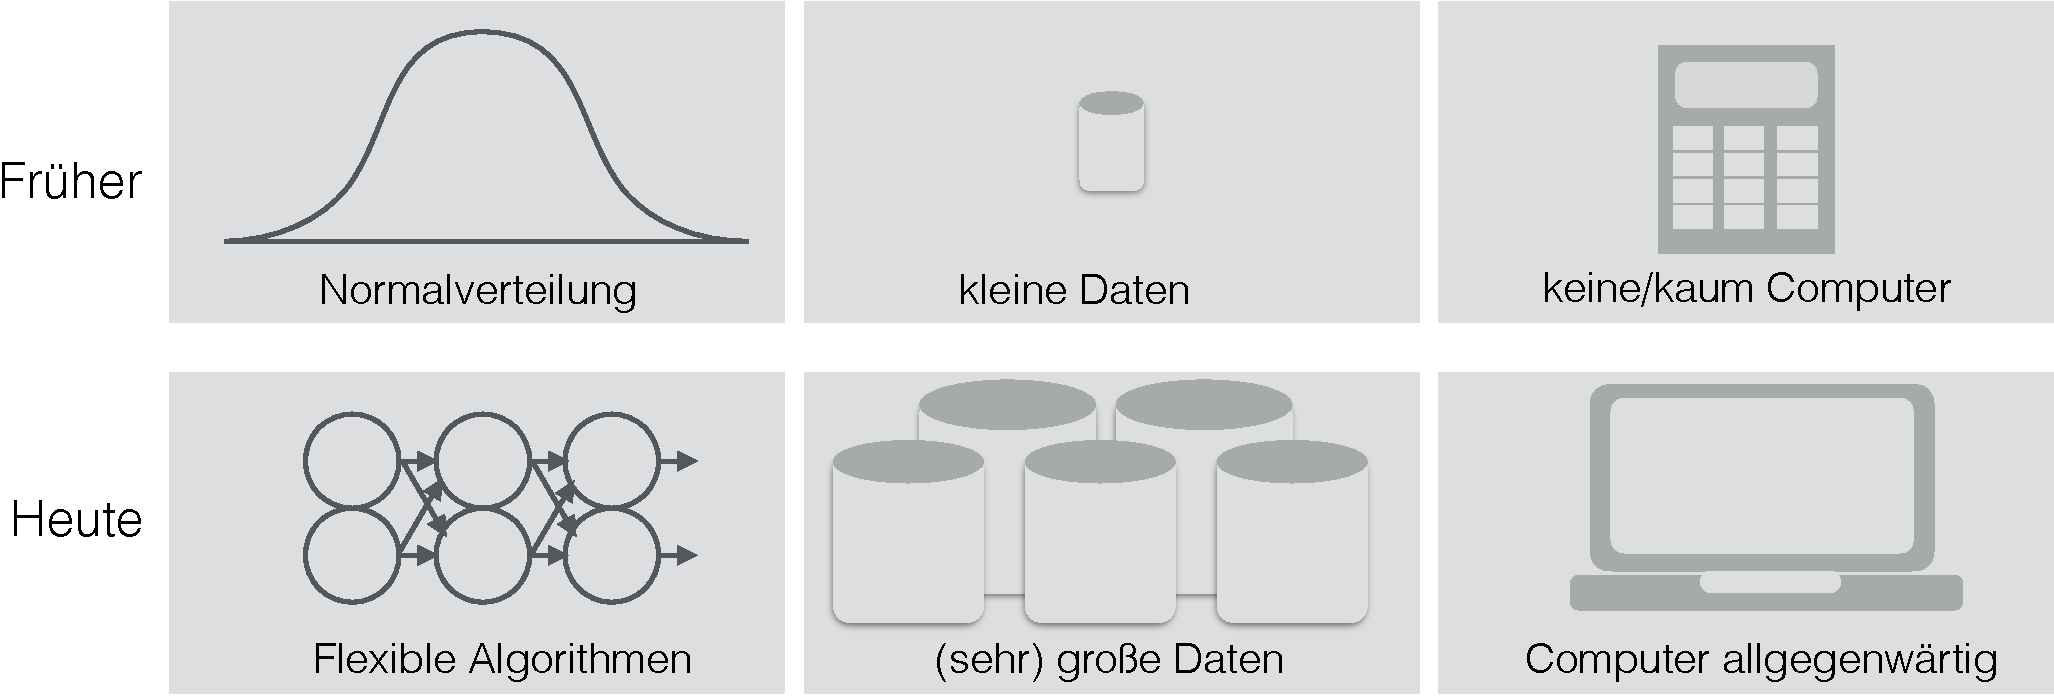
\includegraphics{images/vorwort/Forschung_frueher_heute.pdf}

Zu Themen, die heute zu den dynamischten Gebieten der Datenanalyse
gehören, die aber früher keine große Rolle spielten, gehören (Hardin
u.~a. \protect\hyperlink{ref-hardin2015data}{2015}):

\begin{itemize}
\tightlist
\item
  Nutzung von Datenbanken und anderen Data Warehouses
\item
  Daten aus dem Internet automatisch einlesen (``scraping'')
\item
  Genanalysen mit Tausenden von Variablen
\item
  Gesichtserkennung
\end{itemize}

Sie werden in diesem Kurs einige praktische Aspekte der modernen
Datenanalyse lernen. Ziel ist es, Sie - in Grundzügen - mit der Art und
Weise vertraut zu machen, wie angewandte Statistik bei führenden
Organisationen und Praktikern verwendet wird\footnote{Statistiker, die
  dabei als Vorbild Pate standen sind: Roger D. Peng:
  \url{http://www.biostat.jhsph.edu/~rpeng/}, Hadley Wickham:
  \url{http://hadley.nz}, Jennifer Bryan:
  \url{https://github.com/jennybc}}.

Es ist ein Grundlagenkurs; das didaktische Konzept beruht auf einem
induktiven, intuitiven Lehr-Lern-Ansatz. Formeln und mathematische
Hintergründe such man meist vergebens (tja).

Im Gegensatz zu anderen Statistik-Büchern steht hier die Umsetzung mit R
stark im Vordergrund. Dies hat pragmatische Gründe: Möchte man Daten
einer statistischen Analyse unterziehen, so muss man sie zumeist erst
aufbereiten; oft mühselig aufbereiten. Selten kann man den Luxus
genießen, einfach ``nur'', nach Herzenslust sozusagen, ein Feuerwerk an
multivariater Statistik abzubrennen. Zuvor gilt es, die Daten
aufzubereiten, umzuformen, zu prüfen und zusammenzufassen. Diesem Teil
ist hier recht ausführlich Rechnung getragen.

``Statistical thinking'' sollte, so eine verbreitete Idee, im Zentrum
oder als Ziel einer Statistik-Ausbildung stehen (Wild und Pfannkuch
\protect\hyperlink{ref-wild1999statistical}{1999}). Es ist die Hoffnung
der Autoren dieses Buches, dass das praktische Arbeiten (im Gegensatz zu
einer theoretischen Fokus) zur Entwicklung einer Kompetenz im
statistischen Denken beiträgt.

Außerdem spielt in diesem Kurs die Visualisierung von Daten eine große
Rolle. Zum einen könnte der Grund einfach sein, dass Diagramme
ansprechen und gefallen (einigen Menschen). Zum anderen bieten Diagramme
bei umfangreichen Daten Einsichten, die sonst leicht wortwörtlich
überersehen würden.

\begin{quote}
Dieser Kurs zielt auf die praktischen Aspekte der Analyse von Daten ab:
``wie mache ich es?''; mathematische und philosophische Hintergründe
werden vernachlässigt bzw. auf einschlägige Literatur verwiesen.
\end{quote}

\textbf{Icons}

\emph{R-Pseudo-Syntax}: R ist (momentan) die führende Umgebung für
Datenanalyse. Entsprechend zentral ist R in diesem Kurs. Zugebenermaßen
braucht es etwas Zeit, bis man ein paar Brocken ``Errisch'' spricht. Um
den Einstieg zu erleichern, ist Errisch auf Deutsch übersetzt an einigen
Stellen, wo mir dies besonders hilfreich erschien. Diese Stellen sind
mit diesem Symbol

\includegraphics[width=0.05000\textwidth]{images/pseudocode.png}
gekennzeichnet (für R-Pseudo-Syntax).

\emph{Achtung, Falle}: Schwierige oder fehlerträchtige Stellen sind mit
diesem Symbol

\includegraphics[width=0.05000\textwidth]{images/caution.png} markiert.

\emph{Übungsaufgaben}: Das Skript beinhaltet in jedem Kapitel
Übungsaufgaben oder/und Testfragen. Auf diese wird mit diesem Icon

\includegraphics[width=0.05000\textwidth]{images/exercises.png}
verwiesen oder die Übungen sind in einem Abschnitt mit einsichtigem
Titel zu finden.

\emph{Love}: Wenn Ihnen R diesen Smiley präsentiert, dann sind Sie am
Ziel Ihrer Träume:

\includegraphics[width=0.05000\textwidth]{images/love.png}.

\textbf{Voraussetzungen}

Dieses Buch hat einige \emph{Voraussetzungen}, was das Vorwissen der
Leser angeht; folgende Themengebiete werden vorausgsetzt:

\begin{itemize}
\tightlist
\item
  Deskriptive Statistik
\item
  Grundlagen der Inferenzstatistik
\item
  Grundagen der Regressionsanalyse
\item
  Skalenniveaus
\item
  Grundlagen von R
\end{itemize}

\textbf{Bildnachweise}

Die Bildnachweise sind in folgenden Muster aufgebaut: Nummer, Verweis
zum Bild, Names des Autors, Titel, Quelle (URL), Lizenz, Abrufdatum.

\begin{enumerate}
\def\labelenumi{\arabic{enumi}.}
\item
  Abb. \ref{fig:modellieren-plot}, Sebastian Unrau, ohne Titel,
  \url{https://unsplash.com/photos/CoD2Q92UaEg}, CC0, 2017-02-12.
\item
  Abb. \ref{fig:vwmodell}, Lothar Spurzem, VW 1303 von Wiking in 1:87;
  Größe des Modells: 47,5 mm,
  \url{https://de.wikipedia.org/wiki/Modellautomobil\#/media/File:Wiking-Modell_VW_1303_(um_1975).JPG},
  CC-BY-SA 2.0 de, 2017-03-20.
\item
  ``Icons'' s. oben unter ``Icons'', ``Monster-Smileys'', LadyOfHats,
  Smileys,
  \url{https://commons.wikimedia.org/wiki/User:LadyofHats\#Smileys},
  Public Domain, 2017-01-20.
\item
  Abb. \ref{fig:cecie-une-pipe}, La trahison des images {[}Ceci n'est
  pas une pipe{]}, René Magritte, 1929, © C. Herscovici, Brussels /
  Artists Rights Society (ARS), New York,
  \url{http://collections.lacma.org/node/239578}
\end{enumerate}

\textbf{Lizenz}

Dieses Skript ist publiziert unter
\href{https://creativecommons.org/licenses/by-nc-sa/3.0/de/}{CC-BY-NC-SA
3.0 DE}.

\begin{center}
\includegraphics[width=0.1\linewidth]{images/licence} \end{center}

\textbf{Autoren}

\emph{Sebastian Sauer} schrieb den Hauptteil dieses Buchs. \emph{Oliver
Gansser} schrieb das Kapitel zur Dimensionsreduktion. \emph{Karsten
Lübke} schrieb den Großteil des Kapitels zur Regression und zur
Clusteranalyse sowie Teile des Kapitels `Rahmen'. \emph{Matthias Gehrke}
schrieb den Großteil des Kapitels zur logistischen Regression.

\textbf{Danke}

Norman Markgraf hat umfangreich Fehler gejagt und Verbesserungen
\sout{angemahnt} vorgenommen. Der Austausch mit den ifes-Mitgliedern
hielt die Flamme am Köcheln. Eine Reihe weiterer Kollegen standen mit
Rat und Tat zur Seite. Die Hochschulleitung sowie das Dekanat für
Wirtschaftspsychologie hat dieses Projekt unterstützt. Die Abteilung
Medienentwicklung der FOM hat bei Fragen rund um die Veröffentlichung
geholfen. Last but not least: Viele Studierenden wiesen auf
Inkonsistenzen, Fehler und Unklarheiten hin. Ihnen allen: Vielen Dank!

\textbf{Zitieren}

Bitte zitieren Sie das Skript so:

Sauer, S., Gansser, O. (2017). \emph{Praxis der Datenanalyse}. Skript
zum Modul im MSc.-Studiengang ``Wirtschaftspsychologie \& Consulting''
an der FOM. FOM Nürnberg. DOI: 10.5281/zenodo.580649.

Mehr Infos dazu hier: \url{https://zenodo.org/badge/latestdoi/81811975}

Ein Bib-File finden Sie hier:
\url{https://raw.githubusercontent.com/sebastiansauer/Praxis_der_Datenanalyse/master/Praxis_der_Datenanalyse.bib}.

Alle verwendeten Datensätze und R-Pakete finden sich im
Literaturverzeichnis (genau wie alle zitierten Textstellen).

\textbf{Kontakt}

Wenn Sie einen Fehler oder Verbesserungshinweise berichten möchten,
können Sie unter
\url{https://github.com/sebastiansauer/Praxis_der_Datenanalyse/issues}
einen ``Issue'' einreichen (Button ``New Issue''). Alternativ können Sie
Sebastian Sauer und die anderen Autoren über den Online Campus der FOM
kontaktieren (eine Nachricht schreiben). Sebastian Sauer können Sie via
Twitter folgen (\url{https://twitter.com/sauer_sebastian}) oder seinen
Blog lesen (\url{https://sebastiansauer.github.io}).

\textbf{Technische Details}

Dieses Skript wurde mit dem Paket \texttt{bookdown} (Xie
\protect\hyperlink{ref-xie2015}{2015}) erstellt, welches wiederum stark
auf den Paketen \texttt{knitr} (Xie
\protect\hyperlink{ref-xie2015}{2015}) und \texttt{rmarkdown} (Allaire
u.~a.
\protect\hyperlink{ref-rmarkdown}{2016}\protect\hyperlink{ref-rmarkdown}{a})
beruht. Diese Pakete stellen verblüffende Funktionalität zur Verfügung
als freie Software (frei wie in Bier und frei wie in Freiheit).

Informationen zu den verwendeten Paketen etc. (\texttt{sessionInfo()})
finden Sie hier:
\url{https://raw.githubusercontent.com/sebastiansauer/Praxis_der_Datenanalyse/master/includes/sessionInfo_PraDa.html}.

\textbf{Sonstiges}

Aus Gründen der Lesbarkeit wird das männliche Generikum verwendet,
welches Frauen und Männer in gleichen Maßen ansprechen soll.

Sebastian Sauer

\begin{center}\rule{0.5\linewidth}{\linethickness}\end{center}

\textbf{Herausgeber: FOM Hochschule für Oekonomie \& Management
gemeinnützige GmbH}

Dieses Skript dient als Begleitmaterial zum Modul ``Praxis der
Datenanalyse'' des Masterstudiengangs ``Wirtschaftspsychologie \&
Consulting'' der FOM Hochschule für Oekonomie \& Management.

FOM. Die Hochschule. Für Berufstätige. Die mit bundesweit über 42.000
Studierenden größte private Hochschule Deutschlands führt seit 1993
Studiengang für Berufstätige durch, die einen staatlich und
international anerkannten Hochschulabschluss (Bachelor/Master) erlangen
wollen. Weitere Informationen finden Sie unter
\textless{}www.fom.de\textgreater{}

\newpage

\chapter{Organisatorisches}\label{organisatorisches}

\begin{center}
\includegraphics[width=0.3\linewidth]{images/FOM} \end{center}

\begin{center}
\includegraphics[width=0.1\linewidth]{images/licence} \end{center}

\section{Modulziele}\label{modulziele}

Die Studierenden können nach erfolgreichem Abschluss des Moduls:

\begin{itemize}
\tightlist
\item
  den Ablauf eines Projekts aus der Datenanalyse in wesentlichen
  Schritten nachvollziehen,
\item
  Daten aufbereiten und ansprechend visualisieren,
\item
  Inferenzstatistik anwenden und kritisch hinterfragen,
\item
  klassische Vorhersagemethoden (Regression) anwenden,
\item
  moderne Methoden der angewandten Datenanalyse anwenden (z.B.
  Textmining),
\item
  betriebswirtschaftliche Fragestellungen mittels datengetriebener
  Vorhersagemodellen beantworten.
\end{itemize}

\section{Themen pro Termin}\label{themen-pro-termin}

Für dieses Modul sind 44 UE für Lehre eingeplant, aufgeteilt in 11
Termine (vgl. \ref{tab:termin-themen}).

Folgende Abfolge von Themen sind pro Termin vorgeschlagen:

Tabelle \ref{tab:termin-themen} ordnet die Themen des Moduls den
Therminen (1-11) zu.

\begin{table}

\caption{\label{tab:termin-themen}Zuordnung von Themen zu Terminen}
\centering
\begin{tabular}[t]{r|l}
\hline
Termin & Thema / Kapitel\\
\hline
1 & Organisatorisches\\
\hline
1 & Einführung\\
\hline
1 & Rahmen\\
\hline
1 & Daten einlesen\\
\hline
2 & Datenjudo\\
\hline
3 & Daten visualisieren\\
\hline
4 & Fallstudie\\
\hline
5 & Der p-Wert\\
\hline
5 & Daten modellieren\\
\hline
6 & Lineare Regression - metrisch\\
\hline
7 & Lineare Regression - kategorial\\
\hline
8 & Fallstudie\\
\hline
9 & Vertiefung 1: Textmining oder Clusteranalyse\\
\hline
10 & Vertiefung 2: Baumbasierte Verfahren oder Dimensionsreduktion\\
\hline
11 & Wiederholung\\
\hline
\end{tabular}
\end{table}

\section{Vorerfahrung}\label{vorerfahrung}

Bei den Studierenden werden folgende Themen als bekannt vorausgesetzt:

\begin{itemize}
\tightlist
\item
  Deskriptive Statistik
\item
  Inferenzstatistik
\item
  Grundlagen R
\item
  Grundlagen der Datenvisualisierung
\end{itemize}

\section{Prüfung}\label{prufung}

\subsection{Prüfungshinweise}\label{prufungshinweise}

\begin{itemize}
\tightlist
\item
  Die Prüfung besteht aus zwei Teilen

  \begin{itemize}
  \tightlist
  \item
    einer Klausur (50\% der Teilnote)
  \item
    einer Datenanalyse (50\% der Teilnote).
  \end{itemize}
\end{itemize}

\emph{Prüfungsrelevant} ist der gesamte Stoff aus dem Skript und dem
Unterricht mit folgenden Ausnahmen:

\begin{itemize}
\tightlist
\item
  Inhalte/Abschnitte, die als ``nicht klausurrelevant'' gekennzeichnet
  sind,
\item
  Inhalte/Abschnitte, die als ``Vertiefung'' gekennzeichnet sind,
\item
  Fallstudien (nur für Klausuren nicht prüfungslevant),
\item
  die Inhalte von Links,
\item
  die Inhalte von Fußnoten,
\item
  die Kpaitel \emph{Vorwort}, \emph{Organisatorisches} und
  \emph{Anhang}.
\end{itemize}

\subsection{Klausur}\label{klausur}

\begin{itemize}
\item
  Die Klausur besteht fast oder komplett aus Multiple-Choice
  (MC-)-Aufgaben mit mehreren Antwortoptionen; zumeist ist eine Antwort
  aus vieren auszuwählen.
\item
  Die (maximale) Anzahl der richtigen Aussagen ist pro Aufgabe
  angegeben. Werden mehr Aussagen als ``richtig'' angekreuzt als
  angegeben, so wird die Aufgabe mit 0 Punkten beurteilt. Ansonsten
  werden Teilpunkte für jede Aufgabe vergeben.
\item
  Jede Aussage gilt ceteris paribus (unter sonst gleichen Umständen).
  Aussagen der Art ``A ist B'' (z.B. ``Menschen sind sterblich'') sind
  \emph{nur} dann als richtig auszuwählen, wenn die Aussage \emph{immer}
  richtig ist.
\item
  Im Zweifel ist eine Aussage auf den Stoff, so wie im Unterricht
  behandelt, zu beziehen. Werden in Aussagen Zahlen abgefragt, so sind
  Antworten auch dann richtig, wenn die vorgeschlagene Antwort ab der 1.
  Dezimale von der wahren Antwort abweicht (einigermaßen genaue Aussagen
  werden als richtig akzeptiert). Bei Fragen zu R-Syntax spielen Aspekte
  wie Enter-Taste o.ä. bei der Beantwortung der Frage keine Rolle; diese
  Aspekte dürfen zu ignorieren.
\item
  Jede Aussage einer MC-Aufgabe ist entweder richtig oder falsch (aber
  nicht beides oder keines).
\item
  Die MC-Aufgaben sind nur mit Kreuzen zu beantworten; Text wird bei der
  Korrektur nicht berücksichtigt.
\item
  Bei Nachholklausuren gelten die selben Inhalte (inkl. Schwerpunkte)
  wie bei der Standard-Klausur, sofern nicht anderweitig angegeben.
\item
  I.d.R. sind nur Klausurpapier und ein nicht-programmierbarer
  Taschenrechner als Hilfsmittel zulässig.
\item
  Die Musterlösungen zu offenen Fragen sind elektronisch hinterlegt.
\end{itemize}

\subsection{Datenanalyse}\label{datenanalyse}

\begin{itemize}
\item
  Wenden Sie die passenden, im Modul eingeführten statistischen
  Verfahren an.
\item
  Werten Sie die Daten mit R aus; R-Syntax soll verwendet und im
  Hauptteil dokumentiert werden.
\item
  In der Wahl des Datensatzes sind Sie frei, mit folgender Ausnahme: Im
  Unterricht besprochene Datensätze dürfen nicht als Prüfungsleistung
  eingereicht werden (vgl. Abschnitt \ref{daten}).
\item
  Der (Original-)Name des Datensatzes (sowie ggf. Link) ist bei der
  Anmeldung anzugeben.
\item
  Gruppenarbeiten sind nicht zulässig.
\item
  Hat sich jemand schon für einen Datensatz angemeldet, so darf dieser
  Datensatz nicht mehr gewählt werden (``first come, first serve'').
\item
  Fundorte für Datensätze sind z.B.
  \href{http://www.stat.ufl.edu/~winner/datasets.html}{hier},
  \href{http://archive.ics.uci.edu/ml/datasets.html}{hier} und
  \href{http://vincentarelbundock.github.io/Rdatasets/datasets.html}{hier};
  im Internet finden sich viele Datensätze\footnote{Googeln Sie mal nach
    ``open datasets'' o.ä.}.
\item
  Schreiben Sie Ihre Ergebnisse in einer Ausarbeitung zusammen; der
  Umfang der Ausarbeitung umfasst ca. \emph{1000-1500 Wörter} (nur
  Hauptteil; d.h. exklusive Deckblatt, Verzeichnisse, Anhang etc.).
\item
  Untersuchen Sie 2-3 Hypothesen.
\item
  Denken Sie daran, Name, Matrikelnummer, Modulname etc. anzugeben
  (Deckblatt). Bei der Gestaltung des Layout entscheiden Sie selbständig
  bitte nach Zweckmäßigkeit (und Ästhetik).
\item
  Fügen Sie keine Erklärungen oder Definitionen von statistischen
  Verfahren an.
\end{itemize}

\subsection{Gliederungsvorschlag zur
Datenanalyse}\label{gliederungsvorschlag-zur-datenanalyse}

\begin{enumerate}
\def\labelenumi{\arabic{enumi}.}
\item
  Datensatz

  \begin{enumerate}
  \def\labelenumii{\arabic{enumii}.}
  \item
    Beschreibung

    \begin{itemize}
    \tightlist
    \item
      Name
    \item
      Hintergrund (Themengebiet, Theorien, Relevanz), ca. 100 Wörter
    \item
      Dimension (Zeilen*Spalten)
    \item
      Zitation (wenn vorhanden)
    \item
      sonstige Hinweise (z.B. Datenqualität, Entstehung des Datensatzes)
    \end{itemize}
  \item
    Variablendeskription (nur für Variablen der Hypothese)

    \begin{itemize}
    \tightlist
    \item
      Skalenniveaus
    \item
      Kontinuität (nur bei metrischen Variablen)
    \item
      R-Datentyp
    \item
      Anzahl Fälle und fehlende Werte
    \item
      Erläuterung der Variablen
    \end{itemize}
  \end{enumerate}
\item
  Deduktive Analyse

  \begin{enumerate}
  \def\labelenumii{\arabic{enumii}.}
  \item
    Hypothese(n) Beschreiben Sie die Vermutung(en), die Sie prüfen
    möchten, möglichst exakt.
  \item
    Deskriptive Statistiken

    \begin{itemize}
    \tightlist
    \item
      Berichten Sie deskriptive Statistiken für alle Variablen der
      Hypothesen.
    \item
      Berichten Sie aber nur univariate Statistiken sowie
      Subgruppenanalysen dazu.
    \item
      Berichten Sie ggf. Effektstärken.
    \end{itemize}
  \item
    Diagramme

    \begin{itemize}
    \tightlist
    \item
      Visualisieren Sie Ihre Hypothese(n) bzw. die Daten dazu, gerne aus
      mehreren Blickwinkeln.
    \end{itemize}
  \item
    Signifikanztest
  \end{enumerate}
\item
  Explorative Analyse
\end{enumerate}

\begin{itemize}
\tightlist
\item
  Eörtern Sie interessante Einblicke, die über Ihre vorab getroffenen
  Hypothesen hinausgehen.
\item
  Diagramme können hier eine zentrale Rolle spielen.
\end{itemize}

\begin{enumerate}
\def\labelenumi{\arabic{enumi}.}
\setcounter{enumi}{3}
\item
  Diskussion

  \begin{enumerate}
  \def\labelenumii{\arabic{enumii}.}
  \item
    Zentrale Ergebnisse Fassen Sie das zentrale Ergebnisse zusammen.
  \item
    Interpretation Interpretieren Sie die Ergebnisse: Was bedeuten die
    Zahlen/Fakten, die die Rechnungen ergeben haben?
  \item
    Grenzen der Analyse

    \begin{itemize}
    \tightlist
    \item
      Schildern Sie etwaige Schwachpunkte oder Einschränkungen der
      Analyse.
    \item
      Geben Sie Anregungen für weiterführende Analysen dieses
      Datensatzes.
    \end{itemize}
  \end{enumerate}
\end{enumerate}

\section{Literatur}\label{literatur}

Zum Bestehen der Prüfung ist keine weitere Literatur formal notwendig;
allerdings ist es hilfreich, den Stoff aus unterschiedlichen
Blickwinkeln aufzuarbeiten. Dazu ist am ehesten das Buch von Wickham und
Grolemund (Wickham und Grolemund \protect\hyperlink{ref-r4ds}{2016})
hilreich, obwohl es deutlich tiefer geht als dieses Skript.

\mainmatter

\setcounter{chapter}{0} \part{Grundlagen}

\chapter{Rahmen}\label{rahmen}

\begin{center}
\includegraphics[width=0.3\linewidth]{images/FOM} \end{center}

\begin{center}
\includegraphics[width=0.1\linewidth]{images/licence} \end{center}

\BeginKnitrBlock{rmdcaution}
Lernziele:

\begin{itemize}
\tightlist
\item
  Einen Überblick über die fünf wesentliche Schritte der Datenanalyse
  gewinnen.
\item
  R und RStudio installieren können.
\item
  Einige häufige technische Probleme zu lösen wissen.
\item
  R-Pakete installieren können.
\item
  Einige grundlegende R-Funktionalitäten verstehen.
\item
  Auf die Frage ``Was ist Statistik?'' eine Antwort geben können.
\end{itemize}
\EndKnitrBlock{rmdcaution}

In diesem Skript geht es um die Praxis der Datenanalyse. Mit Rahmen ist
das ``Drumherum'' oder der Kontext der eigentlichen Datenanalyse
gemeint. Dazu gehören einige praktische Vorbereitungen und ein paar
Überlegungen. Zum Beispiel brauchen wir einen Überblick über das Thema.
Voilà (Abb. \ref{fig:fig-prozess}):

\begin{figure}

{\centering 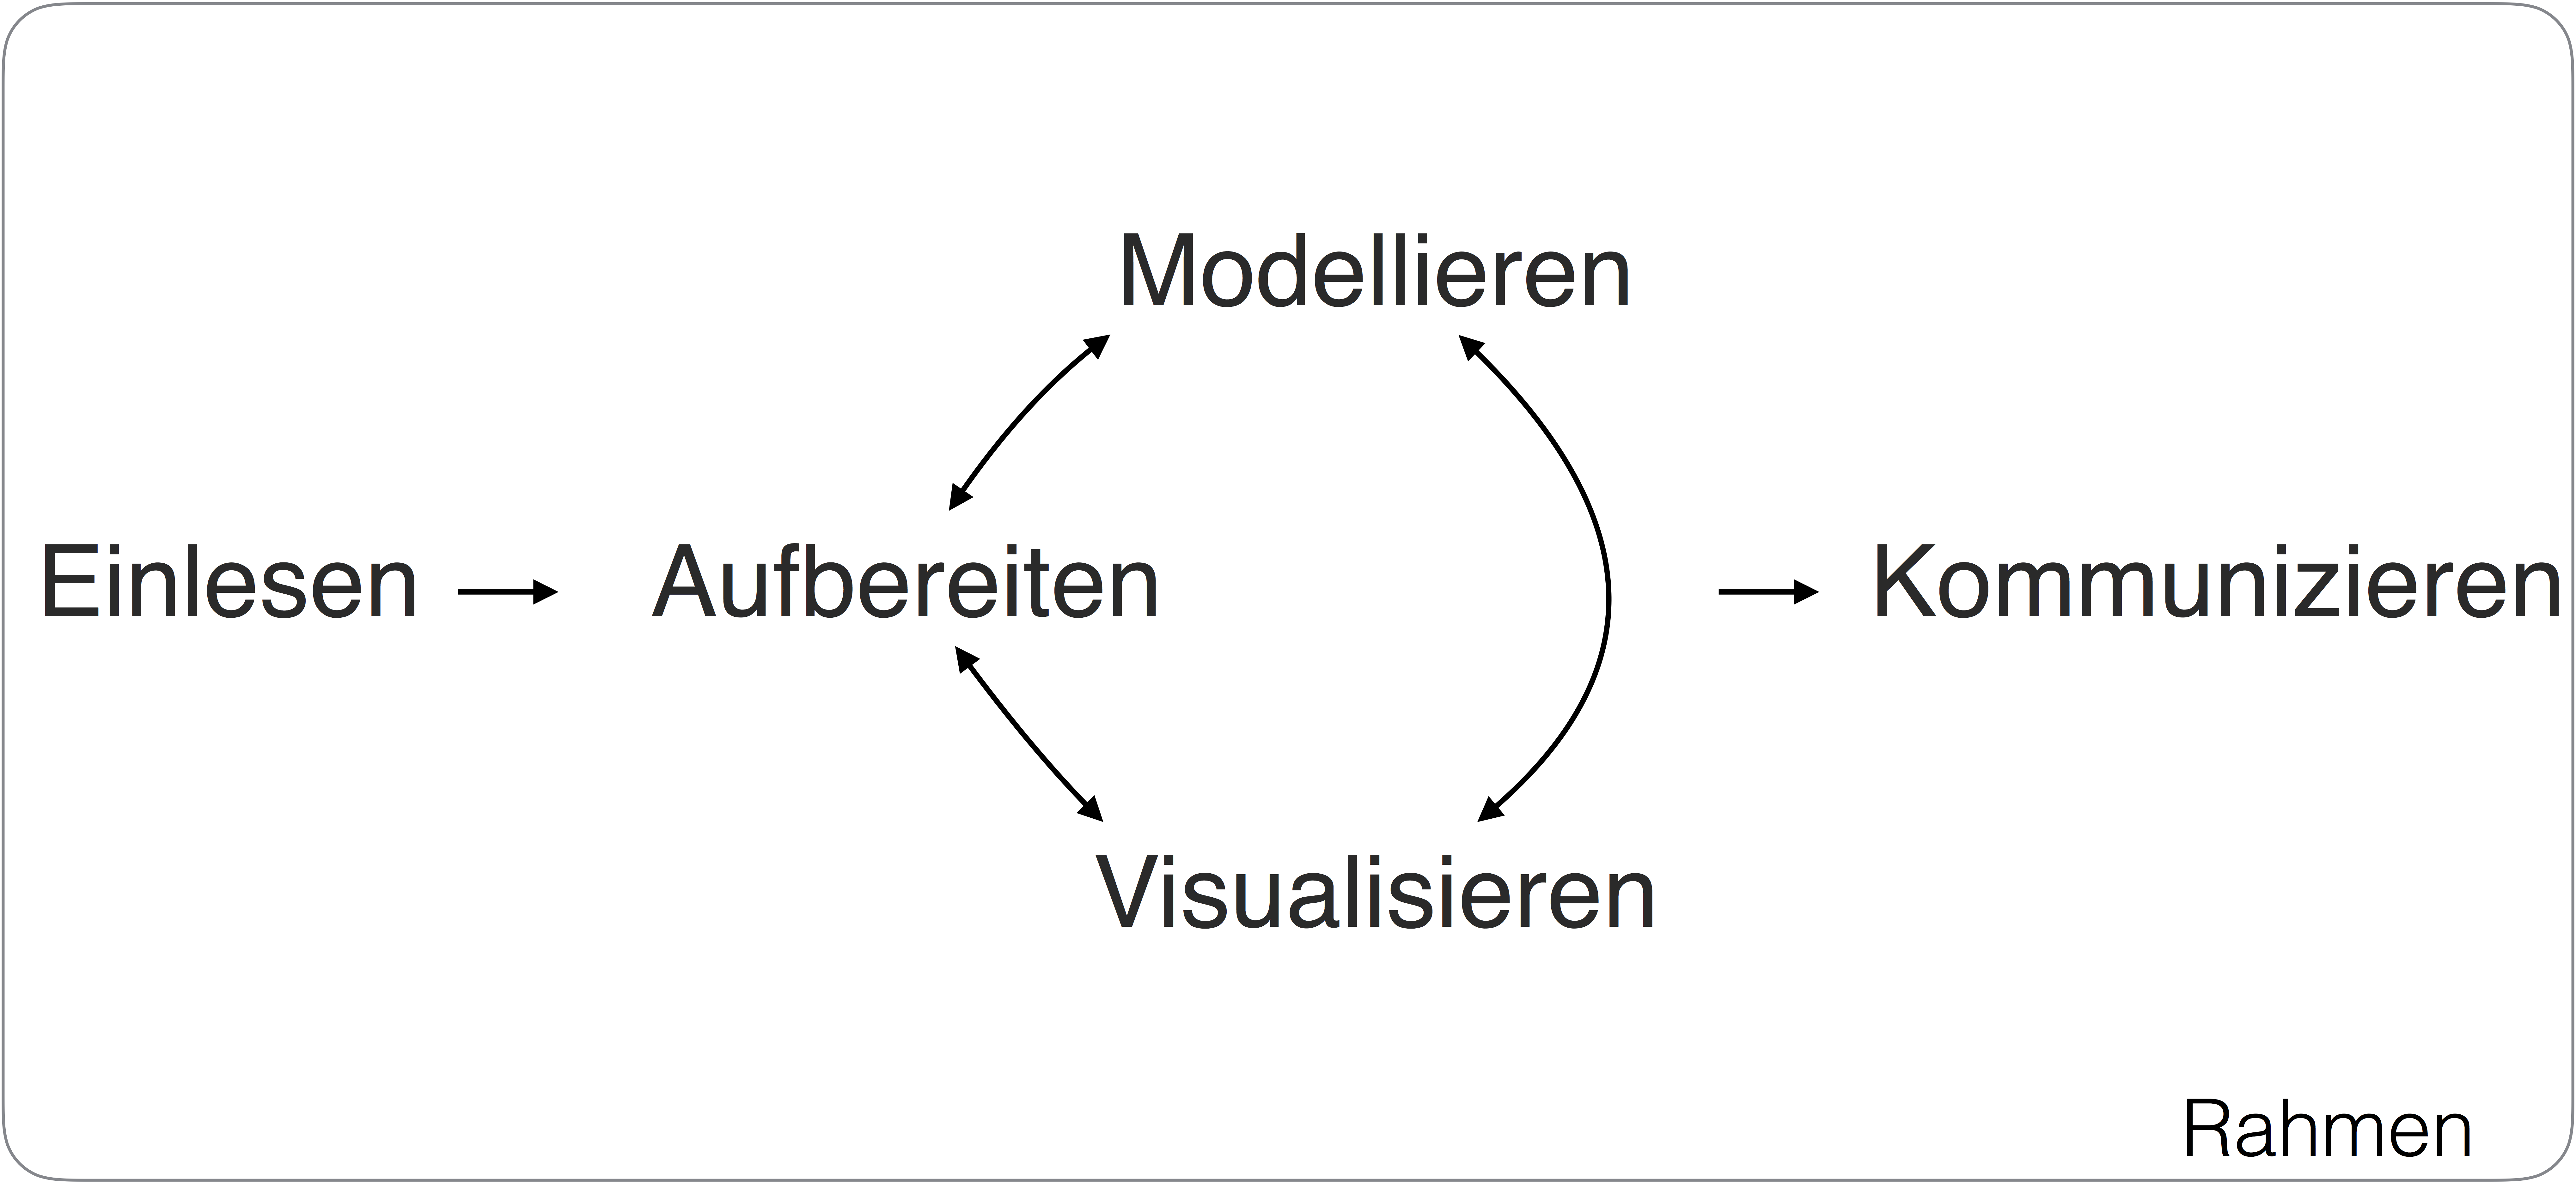
\includegraphics[width=0.7\linewidth]{images/Rahmen/Prozess_Datenanalyse} 

}

\caption{Der Prozess der Datenanalyse}\label{fig:fig-prozess}
\end{figure}

Datenanalyse, praktisch betrachtet, kann man in fünf Schritte einteilen
(Wickham und Grolemund \protect\hyperlink{ref-r4ds}{2016}). Zuerst muss
man die Daten \emph{einlesen}, die Daten also in R (oder einer anderen
Software) verfügbar machen (laden). Fügen wir hinzu: In \emph{schöner
Form} verfügbar machen; man nennt dies auch \emph{tidy data} (hört sich
cooler an). Sobald die Daten in geeigneter Form in R geladen sind, folgt
das \emph{Aufbereiten}. Das beinhaltet Zusammenfassen, Umformen oder
Anreichern je nach Bedarf. Ein nächster wesentlicher Schritt ist das
\emph{Visualisieren} der Daten. Ein Bild sagt bekanntlich mehr als viele
Worte. Schließlich folgt das \emph{Modellieren} oder das Hypothesen
prüfen: Man überlegt sich, wie sich die Daten erklären lassen könnten.
Zu beachten ist, dass diese drei Schritte - Aufbereiten, Visualisieren,
Modellieren - keine starre Abfolge sind, sondern eher ein munteres
Hin-und-Her-Springen, ein aufbauendes Abwechseln. Der letzte Schritt ist
das \emph{Kommunizieren} der Ergebnisse der Analyse - nicht der Daten.
Niemand ist an Zahlenwüsten interessiert; es gilt, spannende Einblicke
zu vermitteln.

Der Prozess der Datenanalyse vollzieht sich nicht im luftleeren Raum,
sondern ist in einem \emph{Rahmen} eingebettet. Dieser beinhaltet
praktische Aspekte - wie Software, Datensätze - und grundsätzliche
Überlegungen - wie Ziele und Grundannahmen.

\section{Software installieren}\label{software-installieren}

Als Haupt-Analysewerkzeug nutzen wir R; daneben wird uns die sog.
``Entwicklungsumgebung'' RStudio einiges an komfortabler Funktionalität
bescheren. Eine Reihe von R-Paketen (``Packages''; d.h. Erweiterungen)
werden wir auch nutzen. R ist eine recht alte Sprache; viele Neuerungen
finden in Paketen Niederschlag, da der ``harte Kern'' von R lieber nicht
so stark geändert wird. Stellen Sie sich vor: Seit 29 Jahren nutzen Sie
eine Befehl, der Ihnen einen Mittelwert ausrechnet, sagen wir die
mittlere Anzahl von Tassen Kaffee am Tag. Und auf einmal wird der
Mittelwert anders berechnet?! Eine Welt stürzt ein! Naja, vielleicht
nicht ganz so tragisch in dem Beispiel, aber grundsätzlich sind
Änderungen in viel benutzen Befehlen potenziell problematisch. Das ist
wohl ein Grund, warum sich am ``R-Kern'' nicht so viel ändert. Die
Innovationen in R passieren in den Paketen. Und es gibt viele davon; als
ich diese Zeilen schreibe, sind es fast schon 10.000! Genauer: 9937 nach
dieser Quelle: \url{https://cran.r-project.org/web/packages/}.

\subsection{R und RStudio
installieren}\label{r-und-rstudio-installieren}


\includegraphics[width=0.20000\textwidth]{images/Rahmen/Rlogo.png}

\includegraphics[width=0.20000\textwidth]{images/Rahmen/rstudiologo.png}

Sie können R unter \url{https://cran.r-project.org} herunterladen und
installieren (für Windows, Mac oder Linux). RStudio finden Sie auf der
gleichnamigen Homepage: \url{https://www.rstudio.com}; laden Sie die
``Desktop-Version'' für Ihr Betriebssystem herunter.

Die Oberfläche von R, die ``Console'', sieht so aus:

Die Oberfläche von RStudio sieht (unter allen Betriebssystemen etwa
gleich) so aus:

\begin{center}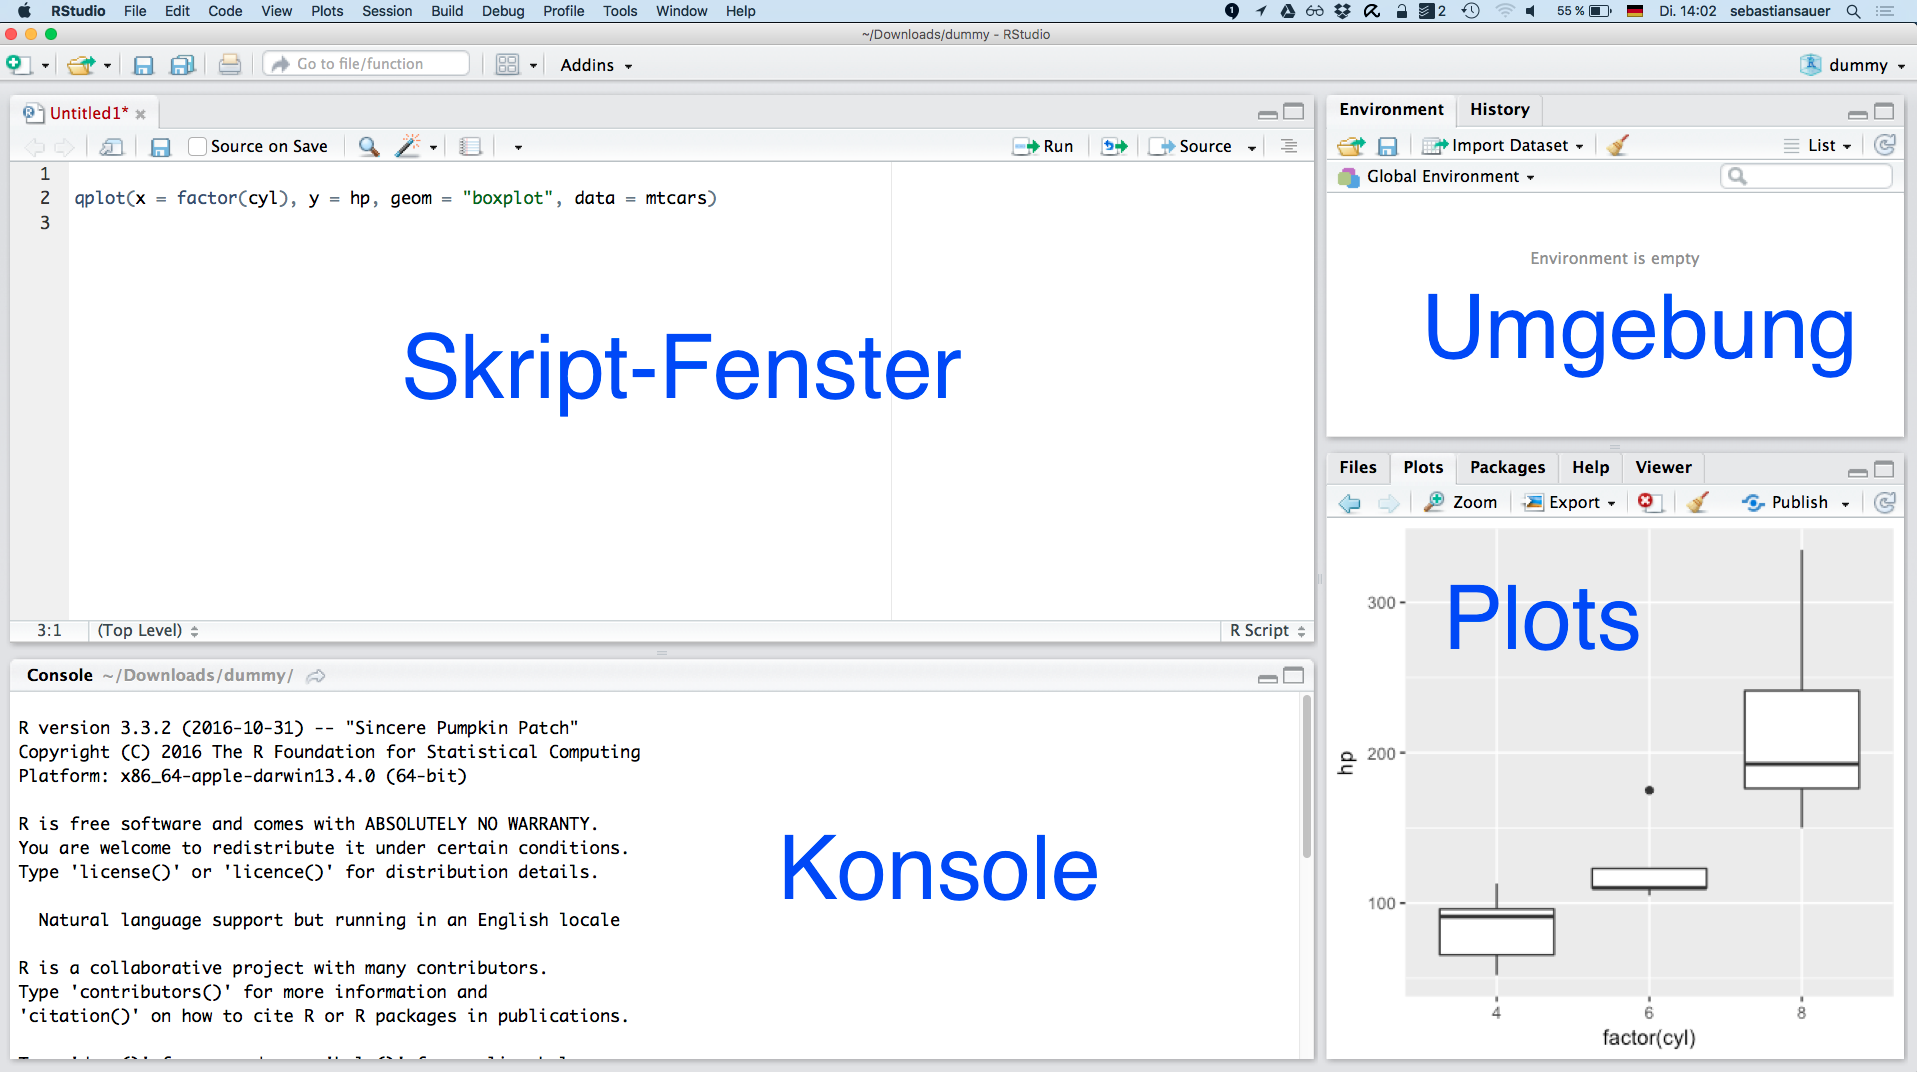
\includegraphics[width=0.7\linewidth]{images/Rahmen/RStudio-Screenshot} \end{center}

Das \emph{Skript-Fenster}\index{Skript-Fenster} ähnelt einem normalem
Text-Editor; praktischerweise finden Sie aber einen Button ``run'', der
die aktuelle Zeile oder die Auswahl ``abschickt'', d.h. in die Konsole
gibt, wo die Syntax ausgeführt wird. Wenn Sie ein Skript-Fenster öffnen
möchten, so können Sie das Icon

\includegraphics{images/Rahmen/new_script.png} klicken (Alternativ:
Ctrl-Shift-N oder File \textgreater{} New File \textgreater{} R Script).

Aus dem Fenster der \emph{Konsole}\index{Konsole} spricht R zu uns bzw.
wir mit R. Wird ein Befehl\index{Funktion} (synonym:
\emph{Funktion}\index{Funktion}) hier eingegeben, so führt R ihn aus. Es
ist aber viel praktischer, Befehle in das Skript-Fenster einzugeben, als
in die Konsole. Behalten Sie dieses Fenster im Blick, wenn Sie Antwort
von R erwarten.

Im Fenster \emph{Umgebung}\index{Umgebung} (engl. ``environment'') zeigt
R, welche Variablen (Objekte) vorhanden sind. Stellen Sie sich die
Umgebung wie einen Karpfenteich vor, in dem die Datensätze und andere
Objekte herumschwimmen. Was nicht in der Umgebung angezeigt wird,
existiert nicht für R.

Im Fenster rechts unten werden mehrere Informationen bereit gestellt,
z.B. werden Diagramme (Plots) dort ausgegeben. Klicken Sie mal die
anderen Reiter im Fenster rechts unten durch.

Wer Shortcuts mag, wird in RStudio überschwänglich beschenkt; der
Shortcut für die Shortcuts ist \texttt{Shift-Alt-K}.

\subsection{Hilfe! R tut nicht so wie ich das
will}\label{hilfe-r-tut-nicht-so-wie-ich-das-will}

\begin{quote}
Manntje, Manntje, Timpe Te,\\
Buttje, Buttje inne See,\\
myne Fru de Ilsebill\\
will nich so, as ik wol will.
\end{quote}

\emph{Gebrüder Grimm, Märchen vom Fischer und seiner Frau\footnote{\url{https://de.wikipedia.org/wiki/Vom_Fischer_und_seiner_Frau}}}

Ihr R startet nicht oder nicht richtig? Die drei wichtigsten Heilmittel
sind:

\begin{enumerate}
\def\labelenumi{\arabic{enumi}.}
\tightlist
\item
  Schließen Sie die Augen für eine Minute. Denken Sie an etwas Schönes
  und was Rs Problem sein könnte.
\item
  Schalten Sie den Rechner aus und probieren Sie es morgen noch einmal.
\item
  Googeln.
\end{enumerate}

Sorry für die schnoddrigen Tipps. Aber: Es passiert allzu leicht, dass
man \emph{Fehler} wie diese macht:

\BeginKnitrBlock{rmdcaution}
OH NO:

\begin{itemize}
\item
  install.packages(dplyr)
\item
  install.packages(``dliar'')
\item
  install.packages(``derpyler'')
\item
  install.packages(``dplyr'') \# dependencies vergessen
\item
  Keine Internet-Verbindung
\item
  library(dplyr) \# ohne vorher zu installieren
\end{itemize}
\EndKnitrBlock{rmdcaution}

Wenn R oder RStudio dann immer noch nicht starten oder nicht richtig
laufen, probieren Sie dieses:

\begin{itemize}
\item
  Sehen Sie eine Fehlermeldung, die von einem fehlenden Paket spricht
  (z.B. ``Package `Rcpp' not available'') oder davon spricht, dass ein
  Paket nicht installiert werden konnte (z.B. ``Package `Rcpp' could not
  be installed'' oder ``es gibt kein Paket namens `Rcpp'\,'' oder
  ``unable to move temporary installation XXX to YYY''), dann tun Sie
  folgendes:
\item
  Schließen Sie R und starten Sie es neu.
\item
  Installieren Sie das oder die angesprochenen Pakete mit
  \texttt{install.packages("name\_des\_pakets",\ dependencies\ =\ TRUE)}
  oder mit dem entsprechenden Klick in RStudio.
\item
  Starten Sie das entsprechende Paket mit
  \texttt{library(name\_des\_pakets)}.
\item
  Gerade bei Windows 10 scheinen die Schreibrechte für R (und damit
  RStudio oder RCommander) eingeschränkt zu sein. Ohne Schreibrechte
  kann R aber nicht die Pakete (``packages'') installieren, die Sie für
  bestimmte R-Funktionen benötigen. Daher schließen Sie R bzw. RStudio
  und suchen Sie das Icon von R oder wenn Sie RStudio verwenden von
  RStudio. Rechtsklicken Sie das Icon und wählen Sie ``als Administrator
  ausführen''. Damit geben Sie dem Programm Schreibrechte. Jetzt können
  Sie etwaige fehlende Pakete installieren.
\item
  Ein weiterer Grund, warum R bzw. RStudio die Schreibrechte verwehrt
  werden könnten (und damit die Installation von Paketen), ist ein
  Virenscanner. Der Virenscanner sagt, nicht ganz zu Unrecht: ``Moment,
  einfach hier Software zu installieren, das geht nicht, zu
  gefährlich''. Grundsätzlich gut, in diesem Fall unnötig. Schließen Sie
  R/RStudio und schalten Sie dann den Virenscanner \emph{komplett} (!)
  aus. Öffnen Sie dann R/RStudio wieder und versuchen Sie fehlende
  Pakete zu installieren.
\end{itemize}

\subsection{Hier werden Sie geholfen}\label{hier-werden-sie-geholfen}

Es ist keine Schande, nicht alle Befehle der ca. 10,000 R-Pakete
auswendig zu wissen. Schlauer ist, zu wissen, wo man Antworten findet.
Hier eine Auswahl:

\begin{itemize}
\item
  Zu diesen Paketen gibt es gute ``Spickzettel'' (cheatsheets): ggplot2,
  RMarkdown, dplyr, tidyr. Klicken Sie dazu in RStudio auf \emph{Help
  \textgreater{} Cheatsheets \textgreater{} \ldots{}} oder gehen Sie auf
  \url{https://www.rstudio.com/resources/cheatsheets/}.
\item
  In RStudio gibt es eine Reihe (viele) von Tastaturkürzeln (Shortcuts),
  die Sie hier finden: \emph{Tools \textgreater{} Keyboard Shortcuts
  Help}.
\item
  Für jeden Befehl (d.i. Funktion) können Sie mit \texttt{?} Hilfe
  erhalten; probieren Sie z.B. \texttt{?mean}.
\item
  Im Internet finden sich zuhauf Tutorials.
\item
  Der Reiter ``Help'' bei RStudio verweist auf die Hilfe-Seite des
  jeweiligen Pakets bzw. Befehls.
\item
  Die bekannteste Seite, um Fragen rund um R zu diskutieren ist
  \url{http://stackoverflow.com}.
\end{itemize}

\subsection{Die Denk- und Gefühlswelt von
R}\label{die-denk--und-gefuhlswelt-von-r}

\begin{itemize}
\tightlist
\item
  Wenn Sie RStudio starten, startet R automatisch auch. Starten Sie
  daher, wenn Sie RStudio gestartet haben, \emph{nicht} noch extra R.
  Damit hätten Sie sonst zwei Instanzen von R laufen, was zu
  Verwirrungen (bei R und beim Nutzer) führen kann.
\end{itemize}

\subsubsection{R-Skript-Dateien}\label{r-skript-dateien}

\begin{itemize}
\item
  Ein neues \emph{R-Skript}\index{R-Skript} im RStudio können Sie z.B.
  öffnen mit \texttt{File-New\ File-R\ Script}. Schreiben Sie dort Ihre
  R-Befehle; Sie können die Skriptdatei speichern, öffnen, ausdrucken,
  übers Bett hängen\ldots{}
\item
  R-Skripte können Sie speichern (unter \texttt{File-Save}) und öffnen.
\item
  R-Skripte sind einfache Textdateien, die jeder Texteditor verarbeiten
  kann. Nur statt der Endung \texttt{.txt}, sind R-Skripte stolzer
  Träger der Endung \texttt{.R}. Es bleibt aber eine schnöde Textdatei.
  Geben Sie Ihren R-Skript-Dateien die Endung ``.R'', damit erkennt
  RStudio, dass es sich um ein R-Skript handelt und bietet ein paar
  praktische Funktionen wie den ``Run-Button''.
\end{itemize}

\subsubsection{Stolpersteine beim Errisch
lernen}\label{stolpersteine-beim-errisch-lernen}

\begin{quote}
I Errr, therefore I am\ldots{}
\end{quote}

Verwenden Sie möglichst die neueste Version von R, RStudio und Ihres
Betriebssystems. Ältere Versionen führen u.U. zu Problemen; je älter,
desto Problem\ldots{} Updaten Sie Ihre Packages regelmäßig z.B. mit
\texttt{update.packages()} oder dem Button ``Update'' bei RStudio
(Reiter \texttt{Packages}).

R zu lernen kann hart sein. Ich weiß, wovon ich spreche. Wahrscheinlich
eine spirituelle Prüfung in Geduld und Hartnäckigkeit\ldots{} Tolle
Gelegenheit, sich in diesen Tugenden zu trainieren :-)

\subsection{Pakete installieren}\label{pakete-installieren}

Ein R-Paket, welches für die praktische Datenanalyse praktisch ist,
heißt \texttt{dplyr}. Wir werden viel mit diesem Paket arbeiten. Bitte
installieren Sie es schon einmal, sofern noch nicht geschehen:

\begin{Shaded}
\begin{Highlighting}[]
\KeywordTok{install.packages}\NormalTok{(}\StringTok{"dplyr"}\NormalTok{, }\DataTypeTok{dependencies =} \OtherTok{TRUE}\NormalTok{) }
\end{Highlighting}
\end{Shaded}

\BeginKnitrBlock{rmdcaution}
Beim Installieren von R-Paketen könnten Sie gefragt werden, welchen
``Mirror'' Sie verwenden möchten. Das hat folgenden Hintergrund:
R-Pakete sind in einer Art ``App-Store'', mit Namen CRAN (Comprehense R
Archive Network) gespeichert. Damit nicht ein armer, kleiner Server
überlastet wird, wenn alle Studis dieser Welt just gerade beschließen,
ein Paket herunterzuladen, gibt es viele Kopien dieses Servers - seine
Spiegelbilder (engl. ``mirrors''). Suchen Sie sich einfach einen aus,
der in der Nähe ist.
\EndKnitrBlock{rmdcaution}

Bei der Installation von Paketen mit
\texttt{install.packages("name\_des\_pakets")} sollte stets der
Parameter \texttt{dependencies\ =\ TRUE} angefügt werden. Also
\texttt{install.packages("name\_des\_pakets",\ dependencies\ =\ TRUE)}.
Hintergrund ist: Falls das zu installierende Paket seinerseits Pakete
benötigt, die noch nicht installiert sind (gut möglich), dann werden
diese sog. ``dependencies'' gleich mitinstalliert (wenn Sie
\texttt{dependencies\ =\ TRUE} setzen).

Sie müssen online sein, um Packages zu installieren.

Nicht vergessen: Installieren muss man eine Software \emph{nur einmal};
\emph{starten} (laden) muss man sie jedes Mal, wenn man sie vorher
geschlossen hat und wieder nutzen möchte:

\begin{Shaded}
\begin{Highlighting}[]
\KeywordTok{library}\NormalTok{(dplyr) }
\end{Highlighting}
\end{Shaded}

Der Befehl bedeutet sinngemäß: ``Hey R, geh in die Bücherei (library)
und hole das Buch (package) dplyr!''.

\BeginKnitrBlock{rmdcaution}
Wann benutzt man bei R Anführungszeichen? Das ist etwas verwirrend im
Detail, aber die Grundegel lautet: wenn man Text anspricht. Im Beispiel
oben ``library(dplyr)'' ist ``dplyr'' hier erst mal für R nichts
Bekanntes, weil noch nicht geladen. Demnach müssten \emph{eigentlich}
Anführungsstriche stehen. Allerdings meinte ein Programmierer, dass es
doch so bequemer ist. Hat er Recht. Aber bedenken Sie, dass es sich um
die Ausnahme einer Regel handelt. Sie können also auch schreiben:
library(``dplyr'') oder library(`dplyr'); geht beides.
\EndKnitrBlock{rmdcaution}

Das Installieren und Starten anderer Pakete läuft genauso ab. Am besten
installieren Sie alle Pakete, die wir in diesem Buch benötigen auf
einmal, dann haben Sie Ruhe.

\subsection{R-Pakete für dieses Buch}\label{r-pakete-fur-dieses-buch}

In diesem Skript verwenden wir die folgenden R-Pakete; diese müssen
installiert sein und geladen. Ggf. benötigen Sie Administrator-Rechte,
um Pakete zu installieren. Virenscanner müssen evtl. ausgestaltet sein.

\begin{verbatim}
#>  [1] "BaylorEdPsych" "broom"         "car"           "caret"        
#>  [5] "cluster"       "corrplot"      "corrr"         "downloader"   
#>  [9] "dplyr"         "GGally"        "ggplot2"       "grid"         
#> [13] "knitr"         "lmtest"        "lsa"           "MBESS"        
#> [17] "modelr"        "nycflights13"  "okcupiddata"   "pdftools"     
#> [21] "png"           "psych"         "ROCR"          "SDMTools"     
#> [25] "SnowballC"     "stringr"       "tidyr"         "tidytext"     
#> [29] "tidyverse"     "wordcloud"
\end{verbatim}

Mit folgenden Befehlen installieren Sie alle Pakete auf einmal. Das ist
ganz praktisch, weil Sie ggf. Aktualisierungen bereits installierter
Pakete bekommen.

\begin{Shaded}
\begin{Highlighting}[]
\KeywordTok{load}\NormalTok{(}\StringTok{"includes/Pakete_fuer_PraDa.Rda"}\NormalTok{)}
\KeywordTok{install.packages}\NormalTok{(packages)}
\end{Highlighting}
\end{Shaded}

Für jedes Kapitel ist angegeben, welches Kapitels jeweils benötigt d.h.
zu ladne sind.

\subsection{Datensätze}\label{daten}

\begin{itemize}
\tightlist
\item
  Datensatz \texttt{profiles} aus dem R-Paket \{okcupiddata\} (Kim und
  Escobedo-Land \protect\hyperlink{ref-kim2015okcupid}{2015}); es
  handelt sich um Daten von einer Online-Singlebörse
\item
  Datensatz \texttt{Wage} aus dem R-Paket \{ISLR\} (James, Witten,
  Hastie, und Tibshirani
  \protect\hyperlink{ref-introstatlearning}{2013}\protect\hyperlink{ref-introstatlearning}{b});
  es handelt sich um Gehaltsdaten von US-amerikanischen Männern
\item
  Datensatz \texttt{inf\_test\_short}, hier herunterzuladen:
  \url{https://osf.io/sjhu} (Sauer
  \protect\hyperlink{ref-Sauer_2017}{2017}\protect\hyperlink{ref-Sauer_2017}{a});
  es handelt sich um Ergebnisse einer Statistikklausur
\item
  Datensatz \texttt{flights} aus dem R-Paket \{nycflights13\} (RITA
  \protect\hyperlink{ref-nycflights13}{2013}); es handelt sich um
  Abflüge von den New Yorker Flughäfen
\item
  Datensatz 'wo\_men`, hier herunterzuladen: \url{https://osf.io/ja9dw}
  (Sauer
  \protect\hyperlink{ref-Sauer_2017a}{2017}\protect\hyperlink{ref-Sauer_2017a}{b});
  es handelt sich um Körper- und Schuhgröße von Studierenden
\item
  Datensatz \texttt{tips} aus dem R-Paket \{reshape2\} (Bryant und Smith
  \protect\hyperlink{ref-bryant1995practical}{1995}); es handelt sich um
  Trinkgelder in einem Restaurant
\item
  Datensatz \texttt{extra}, hier herunterzuladen:
  \url{https://osf.io/4kgzh} (Sauer
  \protect\hyperlink{ref-Sauer_2016}{2016}); es handelt sich die
  Ergebnisse einer Umfrage zu Extraversion
\end{itemize}

Wir verwenden zwei Methoden, um Datensätze in R zu laden.

\begin{itemize}
\tightlist
\item
  Zum einen laden wir Datensätze aus R-Paketen, z.B. aus dem Paket
  \texttt{okcupiddata}. Dazu muss das entsprechende Paket installiert
  und geladen sein. Mit dem Befehl
  \texttt{data(name\_des\_datensatzes,\ package\ =\ "name\_des\_paketes")},
  kann man dann die Daten laden. Das Laden eines Pakets lädt noch
  \emph{nicht} die Daten des Paketes; dafür ist der Befehl \texttt{data}
  zuständig.
\end{itemize}

\begin{Shaded}
\begin{Highlighting}[]
\KeywordTok{library}\NormalTok{(okcupiddata) }
\KeywordTok{data}\NormalTok{(profiles, }\DataTypeTok{package =} \StringTok{"okcupiddata"}\NormalTok{)}
\end{Highlighting}
\end{Shaded}

\begin{itemize}
\tightlist
\item
  Alternativ kann man die Daten als CSV- oder als XLS(X)-Datei
  importieren. Die Datei darf dabei sowohl auf einer Webseite als auch
  lokal (Festplatte, Stick\ldots{}) liegen.
\end{itemize}

\begin{Shaded}
\begin{Highlighting}[]
\NormalTok{Daten <-}\StringTok{ }\KeywordTok{read.csv}\NormalTok{(}\StringTok{"https://sebastiansauer.github.io/data/tips.csv"}\NormalTok{) }
\end{Highlighting}
\end{Shaded}

Wir werden mit beiden Methoden arbeiten und ``on the job'' Details
besprechen.

\subsection{Aufgaben}\label{aufgaben}

\begin{enumerate}
\def\labelenumi{\arabic{enumi}.}
\item
  Öffnen Sie das Cheatsheet für RStudio und machen Sie sich mit dem
  Cheatsheet vertraut.
\item
  Sichten Sie kurz die übrigen Cheatsheets; später werden die Ihnen
  vielleicht von Nutzen sein.
\end{enumerate}

\section{ERRRstkontakt}\label{errrstkontakt}

\subsection{Hinweise}\label{hinweise}

Unser erster Kontakt mit R! Ein paar Anmerkungen vorweg:

\begin{itemize}
\tightlist
\item
  R unterscheidet zwischen Groß- und Kleinbuchstaben, d.h. \texttt{Oma}
  und \texttt{oma} sind zwei verschiedene Dinge für R!
\item
  R verwendet den Punkt \texttt{.} als Dezimaltrennzeichen.
\item
  Fehlende Werte werden in R durch \texttt{NA} kodiert.
\item
  Kommentare werden mit dem Rautezeichen \texttt{\#} eingeleitet; der
  Rest der Zeile von von R dann ignoriert.
\item
  Hilfe zu einem Befehl erhält man über ein vorgestelltes Fragezeichen
  \texttt{?}.
\item
  Zusätzliche Funktionalität kann über Zusatzpakete hinzugeladen werden.
  Diese müssen ggf. zunächst installiert werden.
\item
  \emph{Variablennamen}\index{Variablen} (synonym:
  \emph{Objekte}\index{Objekte}) in R müssen mit Buchstaben beginnen;
  ansonsten dürfen nur Zahlen, Unterstriche \texttt{-} und Minuszeichen
  \texttt{-} enthalten sein. Leerzeichen sind nicht erlaubt.
\item
  Variablen einen Namen zu geben, ist nicht leicht, aber wichtig. Namen
  sollten knapp, aber aussagekräftig sein.
\end{itemize}

\begin{verbatim}
# so nicht:
var
x
dummy
objekt
dieser_name_ist_etwas_lang_vielleicht

# gut:
tips_mw
lm1
\end{verbatim}

Um den Inhalt einer Variablen auszulesen, geben wir einfach den Namen
des Objekts ein (und schicken den Befehl ab).

\subsection{R als Taschenrechner}\label{r-als-taschenrechner}

Auch wenn Statistik nicht Mathe ist, so kann man mit R auch rechnen.
Geben Sie zum Üben die Befehle in der R Konsole hinter der
Eingabeaufforderung \texttt{\textgreater{}} ein und beenden Sie die
Eingabe mit \texttt{Return} bzw. \texttt{Enter}.

\begin{Shaded}
\begin{Highlighting}[]
\DecValTok{4+2} 
\CommentTok{#> [1] 6}
\end{Highlighting}
\end{Shaded}

Das Ergebnis wird direkt angezeigt. Bei

\begin{Shaded}
\begin{Highlighting}[]
\NormalTok{x <-}\StringTok{ }\DecValTok{4+2} 
\end{Highlighting}
\end{Shaded}

erscheint zunächst kein Ergebnis. Über \texttt{\textless{}-} wird der
Variable \texttt{x} der Wert \texttt{4+2} zugewiesen. Wenn Sie jetzt

\begin{Shaded}
\begin{Highlighting}[]
\NormalTok{x }
\end{Highlighting}
\end{Shaded}

eingeben, wird das Ergebnis

\begin{verbatim}
#> [1] 6
\end{verbatim}

angezeigt. Sie können jetzt auch mit \texttt{x} weiterrechnen, z.B.:

\begin{Shaded}
\begin{Highlighting}[]
\NormalTok{x/}\DecValTok{4} 
\CommentTok{#> [1] 1.5}
\end{Highlighting}
\end{Shaded}

Vielleicht fragen Sie sich was die \texttt{{[}1{]}} vor dem Ergebnis
bedeutet. R arbeitet vektororientiert, und die \texttt{{[}1{]}} zeigt
an, dass es sich um das erste (und hier auch letzte) Element des Vektors
handelt.

\subsection{Text und Variablen
zuweisen}\label{text-und-variablen-zuweisen}

Man kann einer Variablen auch Text zuweisen (im Gegensatz zu Zahlen):

\begin{Shaded}
\begin{Highlighting}[]
\NormalTok{y <-}\StringTok{ "Hallo R!"}
\end{Highlighting}
\end{Shaded}

Man kann auch einer Variablen eine andere zuweisen:

\begin{Shaded}
\begin{Highlighting}[]
\NormalTok{y <-}\StringTok{ }\NormalTok{x}
\end{Highlighting}
\end{Shaded}

Wird jetzt y mit dem Inhalt von x überschrieben oder umgekehrt? Der
Zuweisungspfeil \texttt{\textless{}-} macht die Richtung der Zuweisung
ganz klar. Zwar ist in R das Gleichheitszeichen synonym zum
Zuweisungspfeil erlaubt, aber der Zuweisungspfeil macht die Sache
glasklar und sollte daher bevorzugt werden.

Man kann auch einer Variablen \emph{mehr als} einen Wert zuweisen:

\begin{Shaded}
\begin{Highlighting}[]
\NormalTok{x <-}\StringTok{ }\KeywordTok{c}\NormalTok{(}\DecValTok{1}\NormalTok{, }\DecValTok{2}\NormalTok{, }\DecValTok{3}\NormalTok{)}
\end{Highlighting}
\end{Shaded}

Dieser Befehl erzeugt eine ``Spalte'' (einen Vektor). Will man einer
Variablen \emph{mehr als} einen Wert zuweisen, muss man die Werte erst
in einen Vektor ``zusammen binden''; das geht mit dem Befehl \texttt{c}
(vom engl. ``\emph{\textbf{c}ombine}'').

\subsection{Funktionen aufrufen}\label{funktionen-aufrufen}

Um einen ``Befehl'' (präziser: eine Funktion) aufzurufen, geben wir
ihren Namen an und definieren sog. ``Parameter'' in einer runden
Klammer, z.B. so:

\begin{Shaded}
\begin{Highlighting}[]
\NormalTok{wo_men <-}\StringTok{ }\KeywordTok{read.csv}\NormalTok{(}\StringTok{"data/wo_men.csv"}\NormalTok{)}
\end{Highlighting}
\end{Shaded}

Allgemein gesprochen:

\begin{verbatim}
funktionsname(parametername1 = wert1, parametername2 = wert2, ...)
\end{verbatim}

Die drei Punkte \texttt{...} sollen andeuten, dass evtl. weitere
Parameter zu übergeben wären. Die Reihenfolge der Parameter ist egal -
wenn man die Parameternamen anführt. Ansonsten muss man sich an die
Standard-Reihenfolge, die eine Funktion vorgibt halten:

\begin{Shaded}
\begin{Highlighting}[]
\CommentTok{#ok:}
\NormalTok{wo_men <-}\StringTok{ }\KeywordTok{read.csv}\NormalTok{(}\DataTypeTok{file =} \StringTok{"data/wo_men.csv"}\NormalTok{, }\DataTypeTok{header =} \OtherTok{TRUE}\NormalTok{, }\DataTypeTok{sep =} \StringTok{","}\NormalTok{)}
\NormalTok{wo_men <-}\StringTok{ }\KeywordTok{read.csv}\NormalTok{(}\StringTok{"data/wo_men.csv"}\NormalTok{, }\OtherTok{TRUE}\NormalTok{, }\StringTok{","}\NormalTok{)}
\NormalTok{wo_men <-}\StringTok{ }\KeywordTok{read.csv}\NormalTok{(}\DataTypeTok{header =} \OtherTok{TRUE}\NormalTok{, }\DataTypeTok{sep =} \StringTok{","}\NormalTok{, }\DataTypeTok{file =} \StringTok{"data/wo_men.csv"}\NormalTok{)}


\CommentTok{# ohno:}
\NormalTok{wo_men <-}\StringTok{ }\KeywordTok{read.csv}\NormalTok{(}\OtherTok{TRUE}\NormalTok{, }\StringTok{"data/wo_men.csv"}\NormalTok{, }\StringTok{","}\NormalTok{)}
\end{Highlighting}
\end{Shaded}

\subsection{Aufgaben}\label{aufgaben-1}

\begin{enumerate}
\def\labelenumi{\arabic{enumi}.}
\setcounter{enumi}{2}
\tightlist
\item
  Führen Sie diese Syntax aus:
\end{enumerate}

\begin{Shaded}
\begin{Highlighting}[]
\NormalTok{meine_coole_variable <-}\StringTok{ }\DecValTok{10}
\NormalTok{meine_coole_var1able }
\end{Highlighting}
\end{Shaded}

Woher rührt der Fehler?

\begin{enumerate}
\def\labelenumi{\arabic{enumi}.}
\setcounter{enumi}{3}
\tightlist
\item
  Korrigieren Sie die Syntax:
\end{enumerate}

\begin{Shaded}
\begin{Highlighting}[]
\KeywordTok{install.packages}\NormalTok{(dplyer)}
\end{Highlighting}
\end{Shaded}

\texttt{y\ \textless{}-\ Hallo\ R!}

\texttt{Hallo\ R\ \textless{}-\ 1}

\begin{Shaded}
\begin{Highlighting}[]
\NormalTok{Hallo_R <}\StringTok{ }\NormalTok{-}\StringTok{ }\DecValTok{1}
\end{Highlighting}
\end{Shaded}

\section{Was ist Statistik? Wozu ist sie
gut?}\label{was-ist-statistik-wozu-ist-sie-gut}

Zwei Fragen bieten sich sich am Anfang der Beschäftigung mit jedem Thema
an: Was ist die Essenz des Themas? Warum ist das Thema (oder die
Beschäftigung damit) wichtig?

Was ist Statistik? \emph{Eine} Antwort dazu ist, dass Statistik die
Wissenschaft von Sammlung, Analyse, Interpretation und Kommunikation von
Daten ist mithilfe mathematischer Verfahren ist und zur
Entscheidungshilfe beitragen solle (\emph{The Oxford Dictionary of
Statistical Terms} \protect\hyperlink{ref-oxford}{2006}; Romeijn
\protect\hyperlink{ref-sep-statistics}{2016}). Damit hätten wir auch den
Unterschied zur schnöden Datenanalyse (ein Teil der Statistik)
herausgemeißelt. Statistik wird häufig in die zwei Gebiete
\emph{deskriptive} und \emph{inferierende} Statistik eingeteilt. Erstere
fasst viele Zahlen zusammen, so dass wir den Wald statt vieler Bäume
sehen. Letztere verallgemeinert von den vorliegenden (sog.
``Stichproben-'')Daten auf eine zugrunde liegende Grundmenge
(Population). Dabei spielt die Wahrscheinlichkeitsrechnung (Stochastik)
eine große Rolle.

Aufgabe der deskriptiven Statistik ist es primär, Daten prägnant
zusammenzufassen. Aufgabe der Inferenzstatistik ist es, zu prüfen, ob
Daten einer Stichprobe auf eine Grundgesamtheit verallgemeinert werden
können.

Dabei lässt sich der Begriff ``Statistik'' als Überbegriff von
``Datenanalyse'' verstehen, wenn diese Sicht auch nicht von allen
geteilt wird (Grolemund und Wickham
\protect\hyperlink{ref-grolemund2014cognitive}{2014}). In diesem Buch
steht die Aufbereitung, Analyse, Interpretation und Kommunikation von
Daten im Vordergrund. Liegt der Schwerpunkt dieser Aktivitäten bei
computerintensiven Methoden, so wird auch von \emph{Data Science}
gesprochen, wobei der Begriff nicht einheitlich verwendet wird (Wickham
und Grolemund \protect\hyperlink{ref-r4ds}{2016}; Hardin u.~a.
\protect\hyperlink{ref-hardin2015data}{2015})

\emph{Daten} kann man definieren als \emph{Informationen, die in einem
Kontext stehen} (Moore
\protect\hyperlink{ref-moore1990uncertainty}{1990}), wobei eine
numerische Konnotation mitschwingt.

\emph{Modellieren} kann man als \emph{zentrale Aufgabe von Statistik}
begreifen (Cobb \protect\hyperlink{ref-cobb2007introductory}{2007};
Grolemund und Wickham
\protect\hyperlink{ref-grolemund2014cognitive}{2014}). Einfach
gesprochen, bedeutet Modellieren in diesem Sinne, ein mathematisches
Narrativ (``Geschichte'') zu finden, welches als Erklärung für gewisse
Muster in den Daten fungiert; vgl. Kap. \ref{mod1}.

Statistisches Modellieren läuft gewöhnlich nach folgendem Muster ab
(Grolemund und Wickham
\protect\hyperlink{ref-grolemund2014cognitive}{2014}):

\begin{verbatim}
Prämisse 1: Wenn Modell M wahr ist, dann sollten die Daten das Muster D aufweisen.
Prämisse 2: Die Daten weisen das Muster D auf.

---

Konklusion: Daher muss das Modell M wahr sein.
\end{verbatim}

Die Konklusion ist \emph{nicht} zwangsläufig richtig. Es ist falsch zu
sagen, dass dieses Argumentationsmuster - Abduktion (Peirce
\protect\hyperlink{ref-peirce1955abduction}{1955}) genannt - wahre,
sichere Schlüsse (Konklusionen) liefert. Die Konklusion \emph{kann, muss
aber nicht}, zutreffen.

Ein Beispiel: Auf dem Nachhauseweg eines langen Arbeitstags wartet, in
einer dunklen Ecke, ein Mann, der sich als Statistik-Professor vorstellt
und Sie zu einem Glücksspiel einlädt. Sofort sagen Sie zu. Der
Statistiker will 10 Mal eine Münze werfen, er setzt auf Zahl (versteht
sich). Wenn er gewinnt, bekommt er 10\euro{} von Ihnen; gewinnen Sie,
bekommen Sie 11\euro{} von ihm. Hört sich gut an, oder? Nun wirft er die
Münze zehn Mal. Was passiert? Er gewinnt 10 Mal, natürlich (so will es
die Geschichte). Sollten wir glauben, dass er ein Betrüger ist?

Ein Modell, welches wir hier verwenden könnten, lautet: Wenn die Münze
gezinkt ist (Modell M zutrifft), dann wäre diese Datenlage D (10 von 10
Treffern) wahrscheinlich - Prämisse 1. Datenlage D ist tatsächlich der
Fall; der Statistiker hat 10 von 10 Treffer erzielt - Prämisse 2. Die
Daten D ``passen'' also zum Modell M; man entscheidet sich, dass der
Professor ein Falschspieler ist.

Wichtig zu erkennen ist, dass Abduktion mit dem Wörtchen \emph{wenn}
beginnt. Also davon \emph{ausgeht}, dass ein Modell M der Fall ist (der
Professor also tatsächlich ein Betrüger ist). Dass, worüber wir
entscheiden wollen, wird also bereits vorausgesetzt. Gilt also M, wie
gut passen dann die Daten dazu?

\begin{quote}
Wie gut passen die Daten D zum Modell M?
\end{quote}

Das ist die Frage, die hier tatsächlich gestellt bzw. beantwortet wird.

Natürlich ist es keineswegs sicher, \emph{dass} das Modell gilt. Darüber
macht die Abduktion auch keine Aussage. Es könnte also sein, dass ein
anderes Modell zutrifft: Der Professor könnte ein Heiliger sein, der uns
auf etwas merkwürdige Art versucht, Geld zuzuschanzen\ldots{} Oder er
hat einfach Glück gehabt.

\begin{quote}
Statistische Modelle beantworten i.d.R. nicht, wie wahrsheinlich es ist,
dass ein Modell gilt. Statistische Modelle beurteilen, wie gut Daten zu
einem Modell passen.
\end{quote}

Häufig trifft ein Modell eine Reihe von Annahmen, die nicht immer
explizit gemacht werden, aber die klar sein sollten. Z.B. sind die
Münzwürfe unabhängig voneinander? Oder kann es sein, dass sich die Münze
``einschießt'' auf eine Seite? Dann wären die Münzwürfe nicht unabhängig
voneinander. In diesem Fall klingt das reichlich unplausibel; in anderen
Fällen kann dies eher der Fall sein\footnote{Sind z.B. die
  Prüfungsergebnisse von Schülern unabhängig voneinander? Möglicherweise
  haben sie von einem ``Superschüler'' abgeschrieben. Wenn der
  Superschüler viel weiß, dann zeigen die Abschreiber auch gute
  Leistung.}. Auch wenn die Münzwürfe unabhängig voneinander sind, ist
die Wahrscheinlichkeit für Zahl jedes Mal gleich? Hier ist es wiederum
unwahrscheinlich, dass sich die Münze verändert, ihre Masse verlagert,
so dass eine Seite Unwucht bekommt. In anderen Situationen können sich
Untersuchungsobjekte verändern (Menschen lernen manchmal etwas, sagt
man), so dass die Wahrscheinlichkeiten für ein Ereignis unterschiedlich
sein können, man dies aber nicht berücksichtigt.

\section{Befehlsübersicht}\label{befehlsubersicht}

Tabelle \ref{tab:befehle-rahmen} stellt die Befehle dieses Kapitels dar.

\begin{table}

\caption{\label{tab:befehle-rahmen}Befehle des Kapitels 'Rahmen'}
\centering
\begin{tabular}[t]{l|l}
\hline
Paket::Funktion & Beschreibung\\
\hline
install.packages("x") & Installiert Paket "x" (nicht: Paket "X")\\
\hline
library & lädt ein Paket\\
\hline
<- & Weist einer Variablen einen Wert zu\\
\hline
c & erstellt eine Spalte/ einen Vektor\\
\hline
\end{tabular}
\end{table}

Diese Befehle ``wohnen'' alle im Standard-R; es ist für diese Befehle
nicht nötig, zusätzliche Pakete zu installieren/ laden.

\section{Verweise}\label{verweise}

\begin{itemize}
\item
  Chester Ismay erläutert einige Grundlagen von R und RStudio, die für
  Datenanalyse hilfreich sind:
  \url{https://bookdown.org/chesterismay/rbasics/}.
\item
  Roger Peng und Kollegen bieten hier einen Einstieg in Data Science mit
  R: \url{https://bookdown.org/rdpeng/artofdatascience/}
\item
  Wickam und Grolemund (\protect\hyperlink{ref-r4ds}{2016}) geben einen
  hervorragenden Überblick in das Thema dieses Buches; ihr Buch ist sehr
  zu empfehlen.
\item
  Wer einen stärker an der Statistik orientierten Zugang sucht, aber
  ``mathematisch sanft'' behandelt werden möchte, wird bei James et al.
  (\protect\hyperlink{ref-introstatlearning}{2013}\protect\hyperlink{ref-introstatlearning}{b})
  glücklich oder zumindest fündig werden.
\end{itemize}

\chapter{Daten einlesen}\label{daten-einlesen}

\begin{center}
\includegraphics[width=0.3\linewidth]{images/FOM} \end{center}

\begin{center}
\includegraphics[width=0.1\linewidth]{images/licence} \end{center}

\BeginKnitrBlock{rmdcaution}
Lernziele:

\begin{itemize}
\tightlist
\item
  Wissen, was eine CSV-Datei ist.
\item
  Wissen, was UTF-8 bedeutet.
\item
  Erläutern können, was R unter dem ``working directory'' versteht.
\item
  Erkennen können, ob eine Tabelle in Normalform vorliegt.
\item
  Daten aus R hinauskriegen (exportieren).
\end{itemize}
\EndKnitrBlock{rmdcaution}

In diesem Kapitel werden folgende Pakete benötigt:

\begin{Shaded}
\begin{Highlighting}[]
\KeywordTok{library}\NormalTok{(readr)  }\CommentTok{# Daten einlesen}
\end{Highlighting}
\end{Shaded}

Dieses Kapitel beantwortet eine Frage: ``Wie kriege ich Daten in
vernünftiger Form in R hinein?''.

\begin{figure}

{\centering 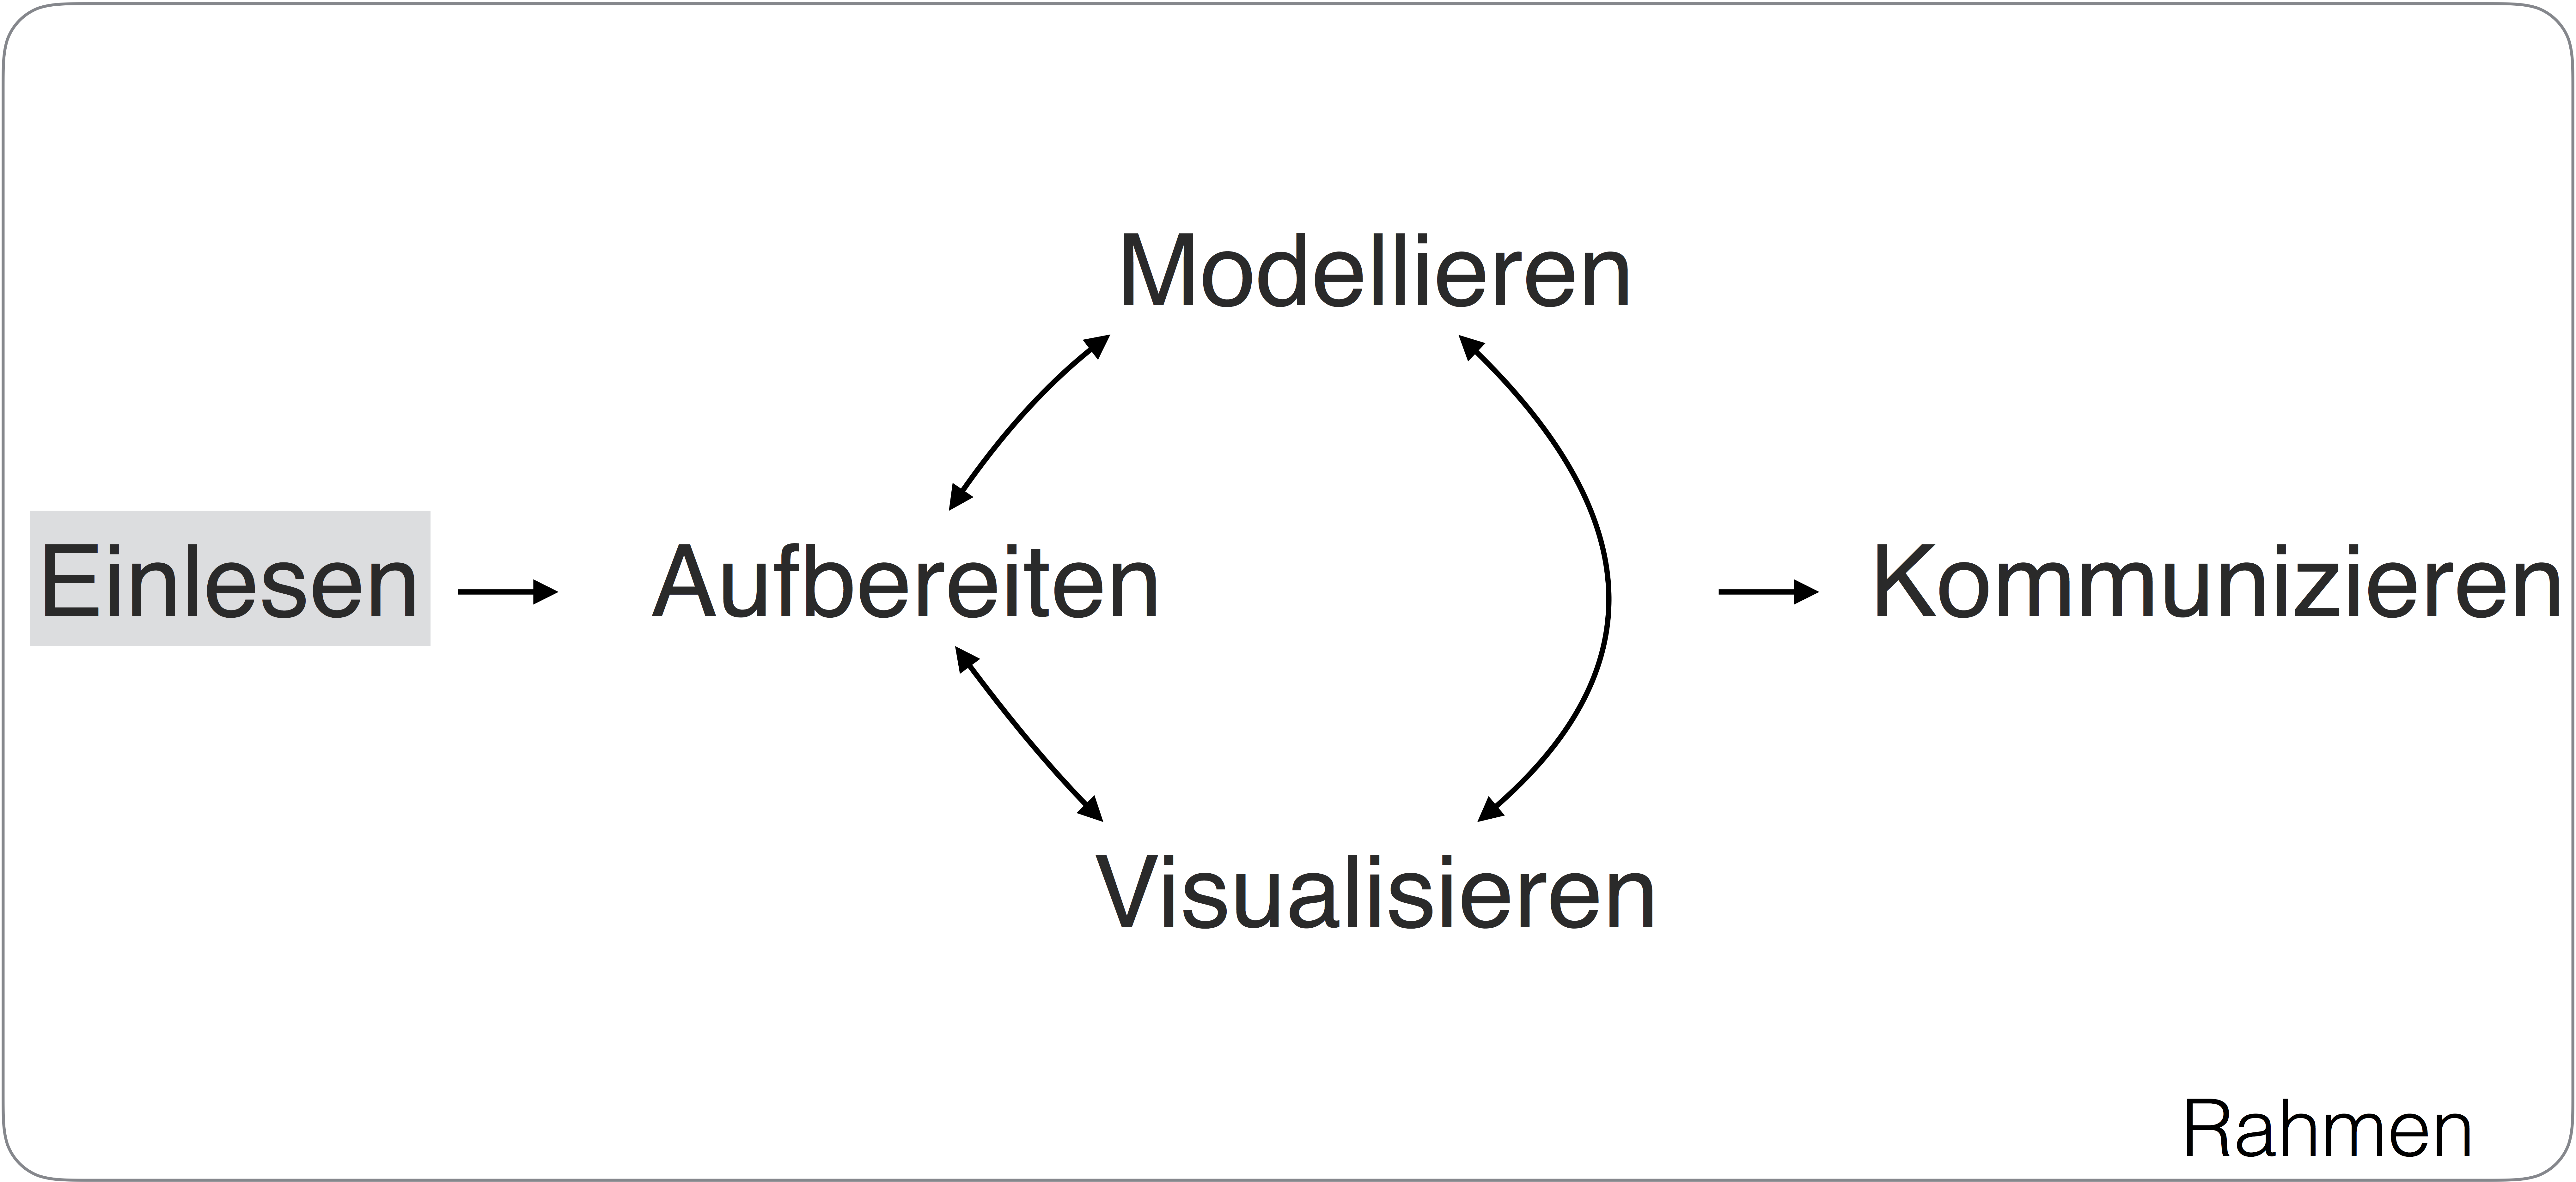
\includegraphics[width=0.7\linewidth]{images/tidy/Einlesen} 

}

\caption{Daten sauber einlesen}\label{fig:step-Einlesen}
\end{figure}

\section{Daten in R importieren}\label{daten-in-r-importieren}

In R kann man ohne Weiteres verschiedene, gebräuchliche (Excel oder CSV)
oder weniger gebräuchliche (Feather\footnote{\url{https://cran.r-project.org/web/packages/feather/index.html}})
Datenformate einlesen. In RStudio lässt sich dies z.B. durch einen
schnellen Klick auf \texttt{Import\ Dataset} im Reiter
\texttt{Environment} erledigen\footnote{Um CSV-Dateien zu laden wird
  durch den Klick im Hintergrund das Paket \texttt{readr} verwendet
  (Wickham, Hester, und Francois
  \protect\hyperlink{ref-readr}{2016}\protect\hyperlink{ref-readr}{a});
  die entsprechende Syntax wird in der Konsole ausgegeben, so dass man
  sie sich anschauen und weiterverwenden kann}.

\subsection{Excel-Dateien importieren}\label{excel-dateien-importieren}

Am einfachsten ist es, eine Excel-Datei (.xls oder .xlsx) über die
RStudio-Oberfläche zu importieren; das ist mit ein paar Klicks
geschehen\footnote{im Hintergrund wird das Paket \texttt{readxl}
  verwendet}:

\begin{figure}

{\centering 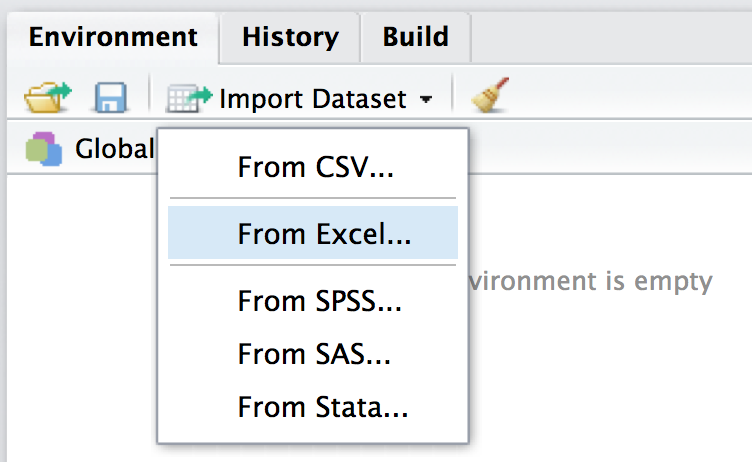
\includegraphics[width=0.5\linewidth]{images/tidy/import_RStudio} 

}

\caption{Daten einlesen (importieren) mit RStudio}\label{fig:data-import-RStudio}
\end{figure}

Es ist für bestimmte Zwecke sinnvoll, nicht zu klicken, sondern die
Syntax einzutippen. Zum Beispiel: Wenn Sie die komplette Analyse als
Syntax in einer Datei haben (eine sog. ``Skriptdatei''), dann brauchen
Sie (in RStudio) nur alles auszuwählen und auf \texttt{Run} zu klicken,
und die komplette Analyse läuft durch! Die Erfahrung zeigt, dass das ein
praktisches Vorgehen ist.

\BeginKnitrBlock{rmdcaution}
Daten (CSV, Excel,\ldots{}) können Sie \emph{nicht} öffnen über
\texttt{File\ \textgreater{}\ Open\ File\ ...}. Dieser Weg ist
Skript-Dateien und R-Daten-Objekten vorbehalten.
\EndKnitrBlock{rmdcaution}

\subsection{CSV-Dateien importieren}\label{csv-dateien-importieren}

Die gebräuchlichste Form von Daten für statistische Analysen ist
wahrscheinlich das CSV-Format. Das ist ein einfaches Format, basierend
auf einer Textdatei. Schauen Sie sich mal diesen Auszug aus einer
CSV-Datei an.

\begin{verbatim}
row_number,date_time,study_time,self_eval,interest,score
1,05.01.2017 13:57:01,5,8,5,29
2,05.01.2017 21:07:56,3,7,3,29
3,05.01.2017 23:33:47,5,10,6,40
4,06.01.2017 09:58:05,2,3,2,18
5,06.01.2017 14:13:08,4,8,6,34
6,06.01.2017 14:21:18,NA,NA,NA,39
\end{verbatim}

Erkennen Sie das Muster? Die erste Zeile gibt die ``Spaltenköpfe''
wieder, also die Namen der Variablen. Hier sind es 6 Spalten; die fünft
heißt ``score'' und gibt die Punkte eines Studierenden in einer
Statistikklausur wieder. Die Spalten sind offenbar durch Komma
\texttt{,} voneinander getrennt. Dezimalstellen sind in amerikanischer
Manier mit einem Punkt \texttt{.} dargestellt. Die Daten sind
``rechteckig''; alle Spalten haben gleich viele Zeilen und umgekehrt
alle Spalten gleich viele Zeilen. Man kann sich diese Tabelle gut als
Excel-Tabelle mit Zellen vorstellen, in denen z.B. ``row\_number''
(Zelle oben links) oder ``39'' (Zelle unten rechts) steht.

An einigen Stelle steht \texttt{NA}. Das ist Errisch für ``fehlender
Wert''. Häufig wird die Zelle auch leer gelassen, um auszudrücken, dass
ein Wert hier fehlt (hört sich nicht ganz doof an). Aber man findet alle
möglichen Ideen, um fehlende Werte darzustellen. Ich rate von allen
anderen ab; führt nur zu Verwirrung.

Lesen wir diese Daten jetzt ein:

\begin{Shaded}
\begin{Highlighting}[]
\NormalTok{df <-}\StringTok{ }\KeywordTok{read.csv}\NormalTok{(}\StringTok{"data/test_inf_short.csv"}\NormalTok{)}
\end{Highlighting}
\end{Shaded}

\subsubsection{Vorsicht bei nicht-amerikanisch kodierten
Textdateien}\label{vorsicht-bei-nicht-amerikanisch-kodierten-textdateien}

Der Befehl \texttt{read.csv} liest also eine CSV-Datei, was uns jetzt
nicht übermäßig überrascht. Aber Achtung: Wenn Sie aus einem Excel mit
\emph{deutscher} Einstellung eine CSV-Datei exportieren, wird diese
CSV-Datei als Spaltentrennung \texttt{;} (Strichpunkt) und als
Dezimaltrennzeichen \texttt{,} verwenden. Da der Befehl
\texttt{read.csv} laut amerikanischen Standard mit Komma als
Spaltentrennung und Punkt als Dezimaltrennzeichen arbeitet, müssen wir
die deutschen Sonderlocken explizit angeben, z.B. so:

\begin{Shaded}
\begin{Highlighting}[]
\CommentTok{# nicht ausführen:}
\NormalTok{daten_deutsch <-}\StringTok{ }\KeywordTok{read.csv}\NormalTok{(}\StringTok{"daten_deutsch.csv"}\NormalTok{, }\DataTypeTok{sep =} \StringTok{";"}\NormalTok{, }\DataTypeTok{dec =} \StringTok{"."}\NormalTok{)}
\end{Highlighting}
\end{Shaded}

Dabei steht \texttt{sep} (separator) für das Trennzeichen zwischen den
Spalten und \texttt{dec} für das Dezimaltrennzeichen. R bietet eine
Kurzfassung für \texttt{read.csv} mit diesen Parametern:
\texttt{read.csv2("daten\_deutsch.csv")}.

Man kommt hier auch mit ``Klicken statt Tippen'' zum Ziel; in der Maske
von ``Import Dataset'' (für CSV-Dateien) gibt es den Auswahlpunkt
``Delimiter'' (Trennzeichen). Dort kann man das Komma durch einen
Strichkpunkt (oder was auch immer) ersetzen. Es hilft, im Zweifel, die
Textdatei vorab mit einem Texteditor zu öffnen.

\begin{figure}

{\centering 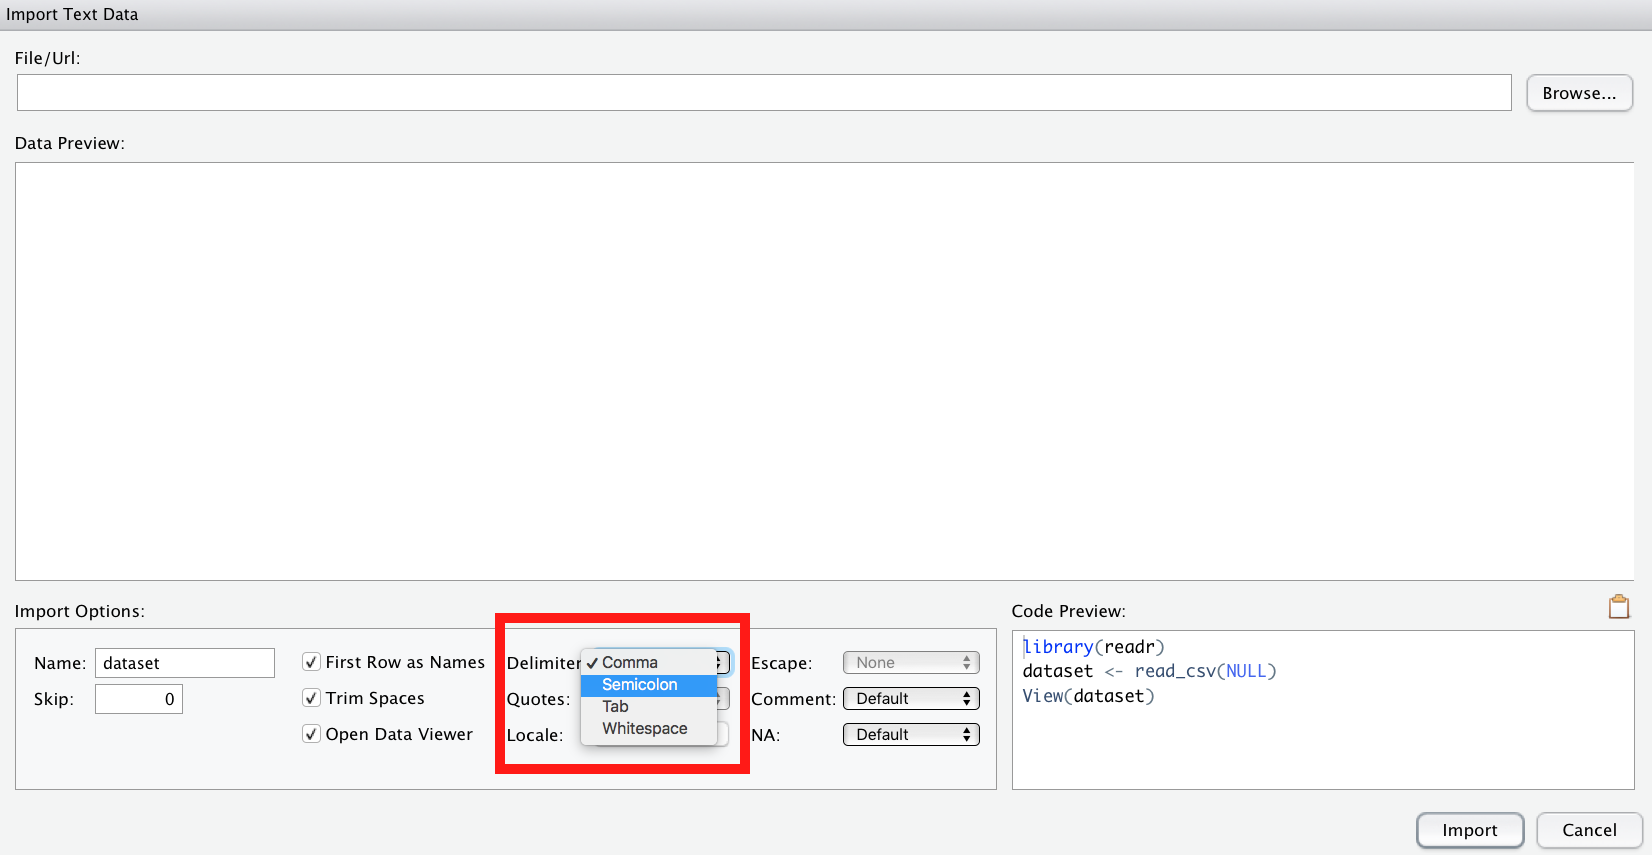
\includegraphics[width=0.7\linewidth]{images/tidy/delimiter} 

}

\caption{Trennzeichen einer CSV-Datei in RStudio einstellen}\label{fig:rstudio-delimiter}
\end{figure}

\subsection{Das Arbeitsverzeichnis}\label{das-arbeitsverzeichnis}

\BeginKnitrBlock{rmdcaution}
Übrigens: Wenn Sie keinen Pfad angeben, so geht R davon aus, dass die
Daten im aktuellen Verzeichnis (dem \emph{working directory}) liegen.
\EndKnitrBlock{rmdcaution}

Das aktuelle Verzeichnis (Arbeitsverzeichnis; ``working directory'')
kann man mit \texttt{getwd()} erfragen und mit \texttt{setwd()}
einstellen. Komfortabler ist es aber, das aktuelle Verzeichnis per Menü
zu ändern. In RStudio:
\texttt{Session\ \textgreater{}\ Set\ Working\ Directory\ \textgreater{}\ Choose\ Directory\ ...}
(oder per Shortcut, der dort angezeigt wird).

Es ist praktisch, das Arbeitsverzeichnis festzulegen, denn dann kann man
z.B. eine Datendatei einlesen, ohne den Pfad eingeben zu müssen:

\begin{Shaded}
\begin{Highlighting}[]
\CommentTok{# nicht ausführen:}
\NormalTok{daten_deutsch <-}\StringTok{ }\KeywordTok{read.csv}\NormalTok{(}\StringTok{"daten_deutsch.csv"}\NormalTok{, }\DataTypeTok{sep =} \StringTok{";"}\NormalTok{, }\DataTypeTok{dec =} \StringTok{"."}\NormalTok{)}
\end{Highlighting}
\end{Shaded}

R geht dann davon aus, dass sich die Datei \texttt{daten\_deutsch.csv}
im Arbeitsverzeichnis befindet.

\section{Normalform einer Tabelle}\label{normalform-einer-tabelle}

Tabellen in R werden als \texttt{data\ frames} (``Dataframe'' auf
Denglisch; moderner: als \texttt{tibble}, Tibble kurz für ``Table-df'')
bezeichnet. Tabellen sollten in ``Normalform'' vorliegen (``tidy''),
bevor wir weitere Analysen starten. Unter Normalform verstehen sich
folgende Punkte:

\begin{itemize}
\tightlist
\item
  Es handelt sich um einen Dataframe, also um eine Tabelle mit Spalten
  mit Namen und gleicher Länge; eine Datentabelle in rechteckiger Form
  und die Spalten haben einen Namen.
\item
  In jeder Zeile steht eine Beobachtung, in jeder Spalte eine Variable.
\item
  Fehlende Werte sollten sich in \emph{leeren} Zellen niederschlagen.
\item
  Daten sollten nicht mit Farbmarkierungen o.ä. kodiert werden.
\item
  Es gibt keine Leerzeilen und keine Leerspalten.
\item
  In jeder Zelle steht ein Wert.
\item
  Am besten verwendet man keine Sonderzeichen verwenden und keine
  Leerzeichen in Variablennamen und -werten, sondern nur Ziffern und
  Buchstaben und Unterstriche.
\item
  Variablennamen dürfen nicht mit einer Zahl beginnen.
\end{itemize}

Abbildung \ref{fig:tidy1} visualisiert die Bestimmungsstücke eines
Dataframes (Wickham und Grolemund \protect\hyperlink{ref-r4ds}{2016}):

\begin{figure}

{\centering 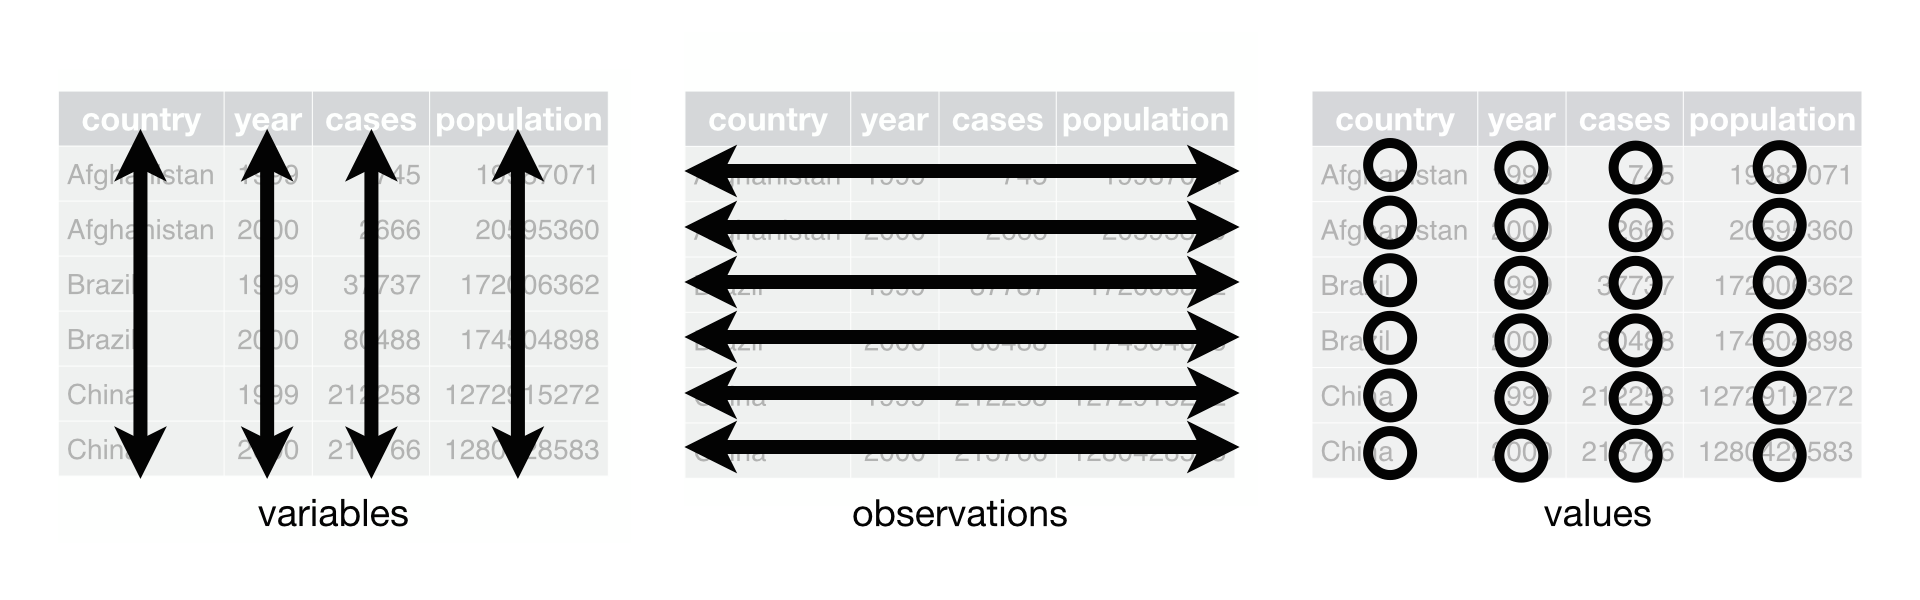
\includegraphics[width=0.7\linewidth]{images/tidy/tidy-1} 

}

\caption{Schematische Darstellung eines Dataframes in Normalform}\label{fig:tidy1}
\end{figure}

Der Punkt \emph{Jede Zeile eine Beobachtung, jede Spalte eine Variable,
jede Zelle ein Wert} verdient besondere Beachtung. Betrachten Sie dieses
Beispiel:

\begin{figure}

{\centering 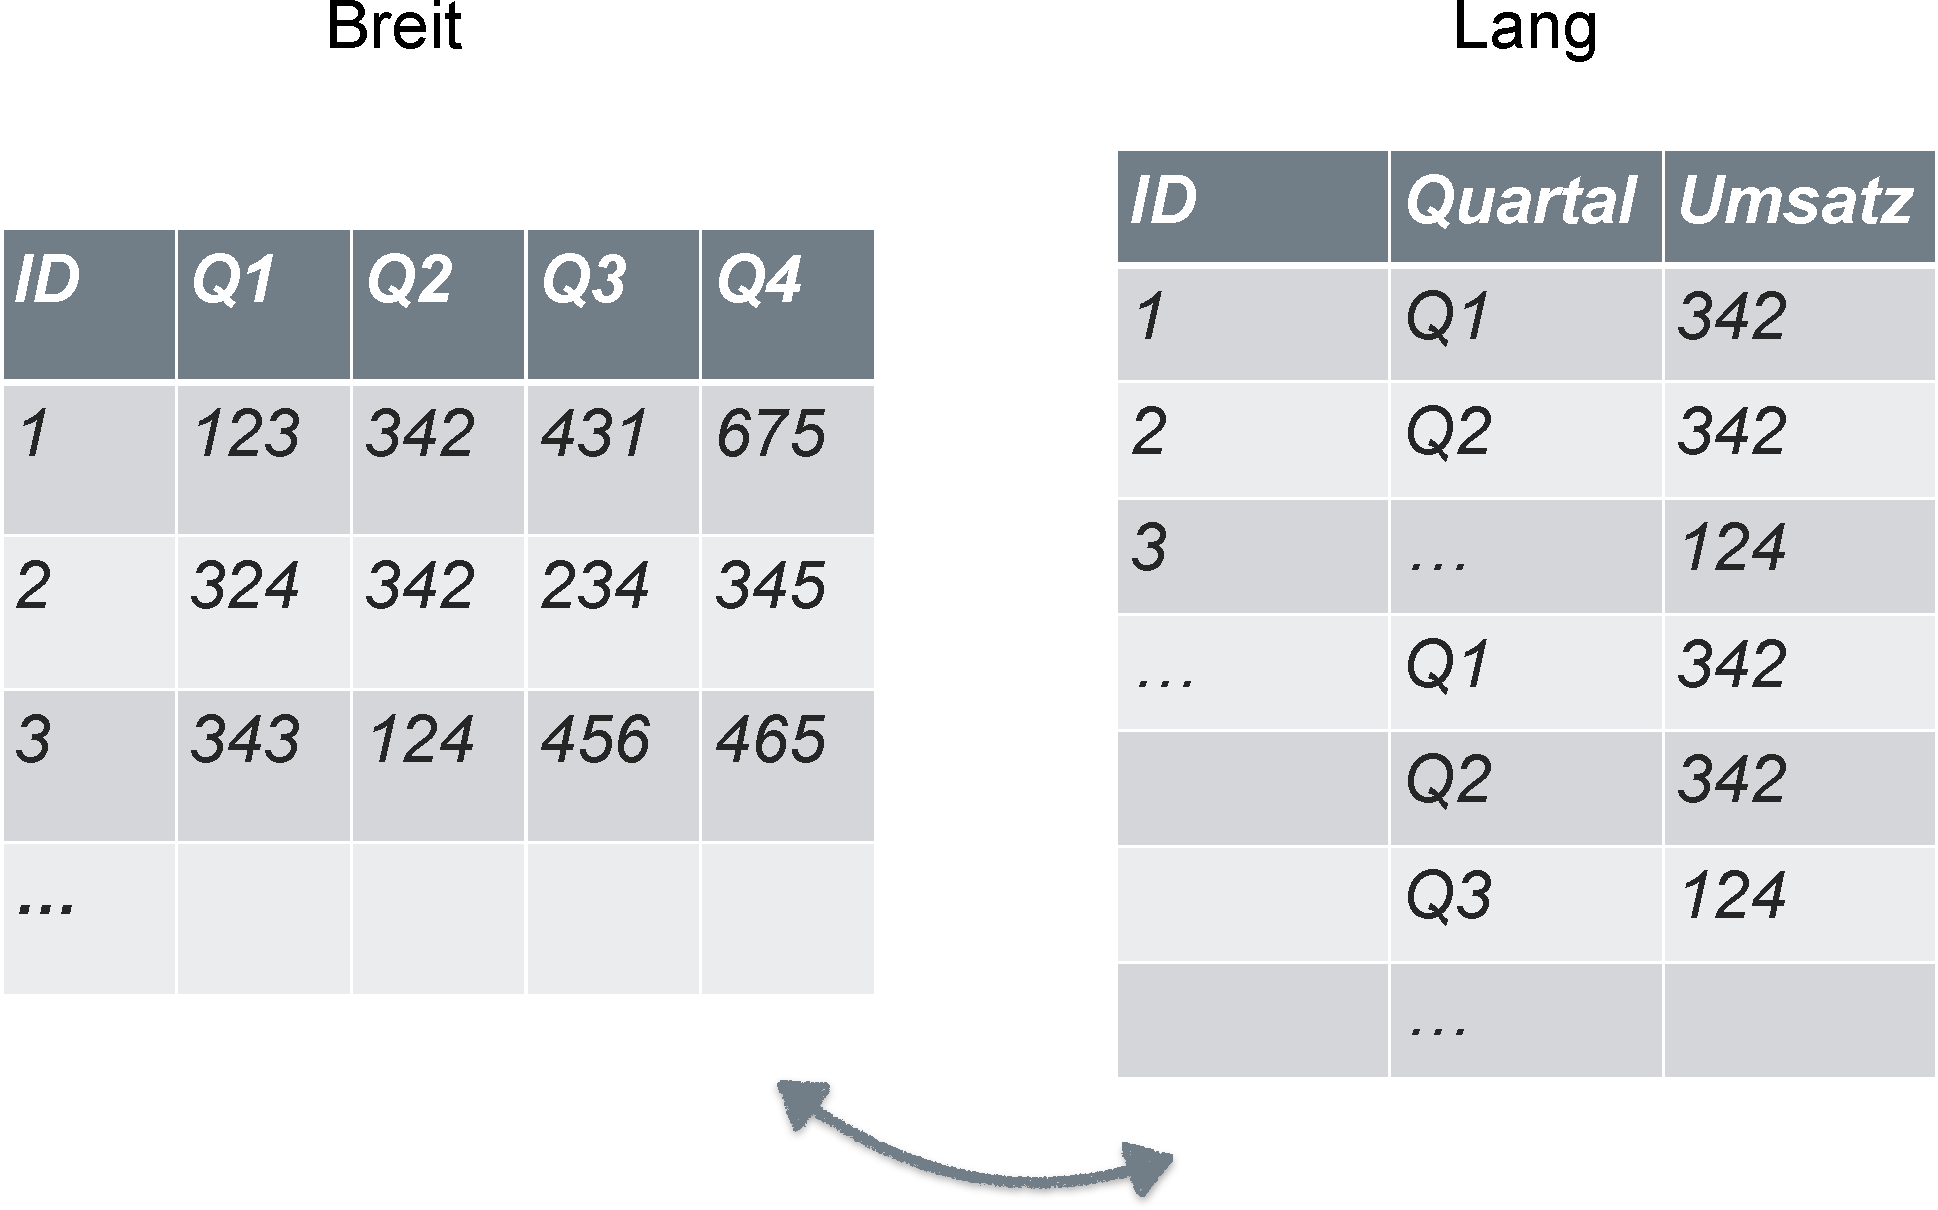
\includegraphics[width=0.7\linewidth]{images/tidy/breit_lang} 

}

\caption{Dieselben Daten - einmal breit, einmal lang}\label{fig:lang-breit}
\end{figure}

In der rechten Tabelle sind die Variablen \texttt{Quartal} und
\texttt{Umsatz} klar getrennt; jede hat ihre eigene Spalte. In der
linken Tabelle hingegen sind die beiden Variablen vermischt. Sie haben
nicht mehr ihre eigene Spalte, sondern sind über vier Spalten verteilt.
Die rechte Tabelle ist ein Beispiel für eine Tabelle in Normalform, die
linke nicht.

\begin{figure}

{\centering 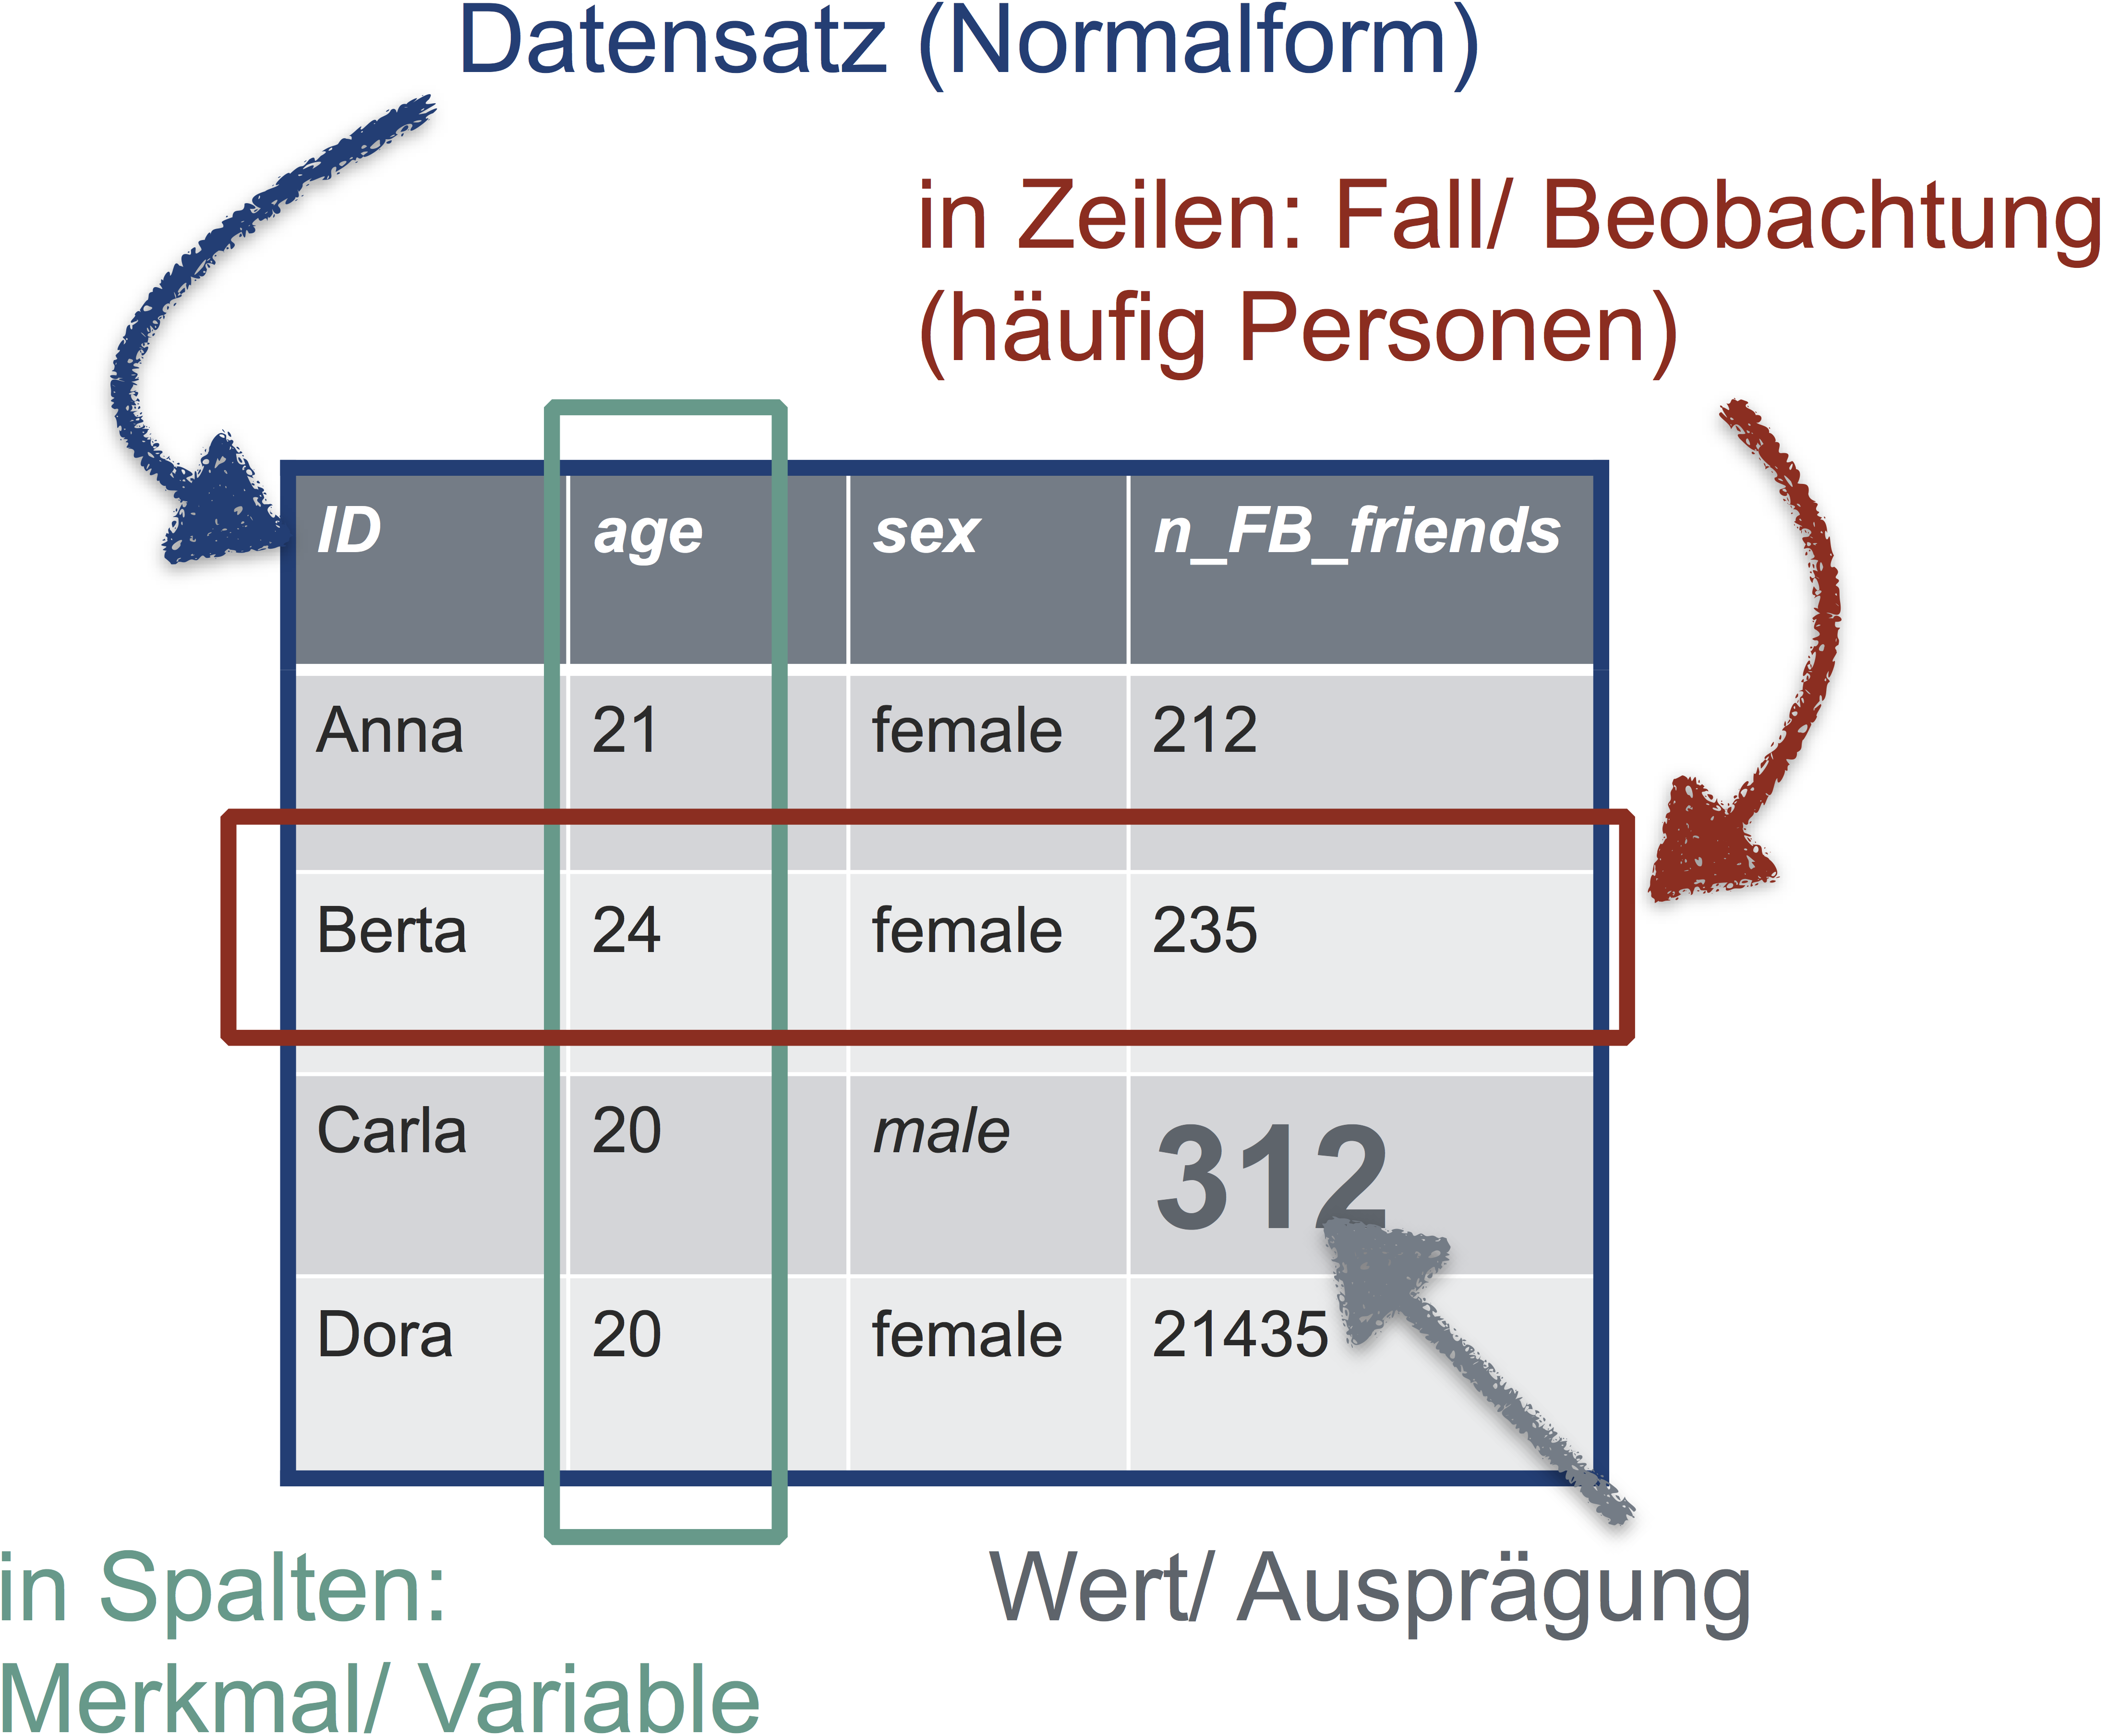
\includegraphics[width=0.7\linewidth]{images/tidy/Normalform} 

}

\caption{Illustration eines Datensatzes in Normalform}\label{fig:fig-Normalform}
\end{figure}

\section{Tabelle in Normalform bringen}\label{normalform}

Eine der ersten Aktionen einer Datenanalyse sollte also die
``Normalisierung'' Ihrer Tabelle sein. In R bietet sich dazu das Paket
\texttt{tidyr} an, mit dem die Tabelle von \emph{Breit- auf Langformat}
(und wieder zurück) geschoben werden kann.

Abb. \ref{fig:gather-spread} zeigt ein Beispiel dazu.

\begin{figure}

{\centering 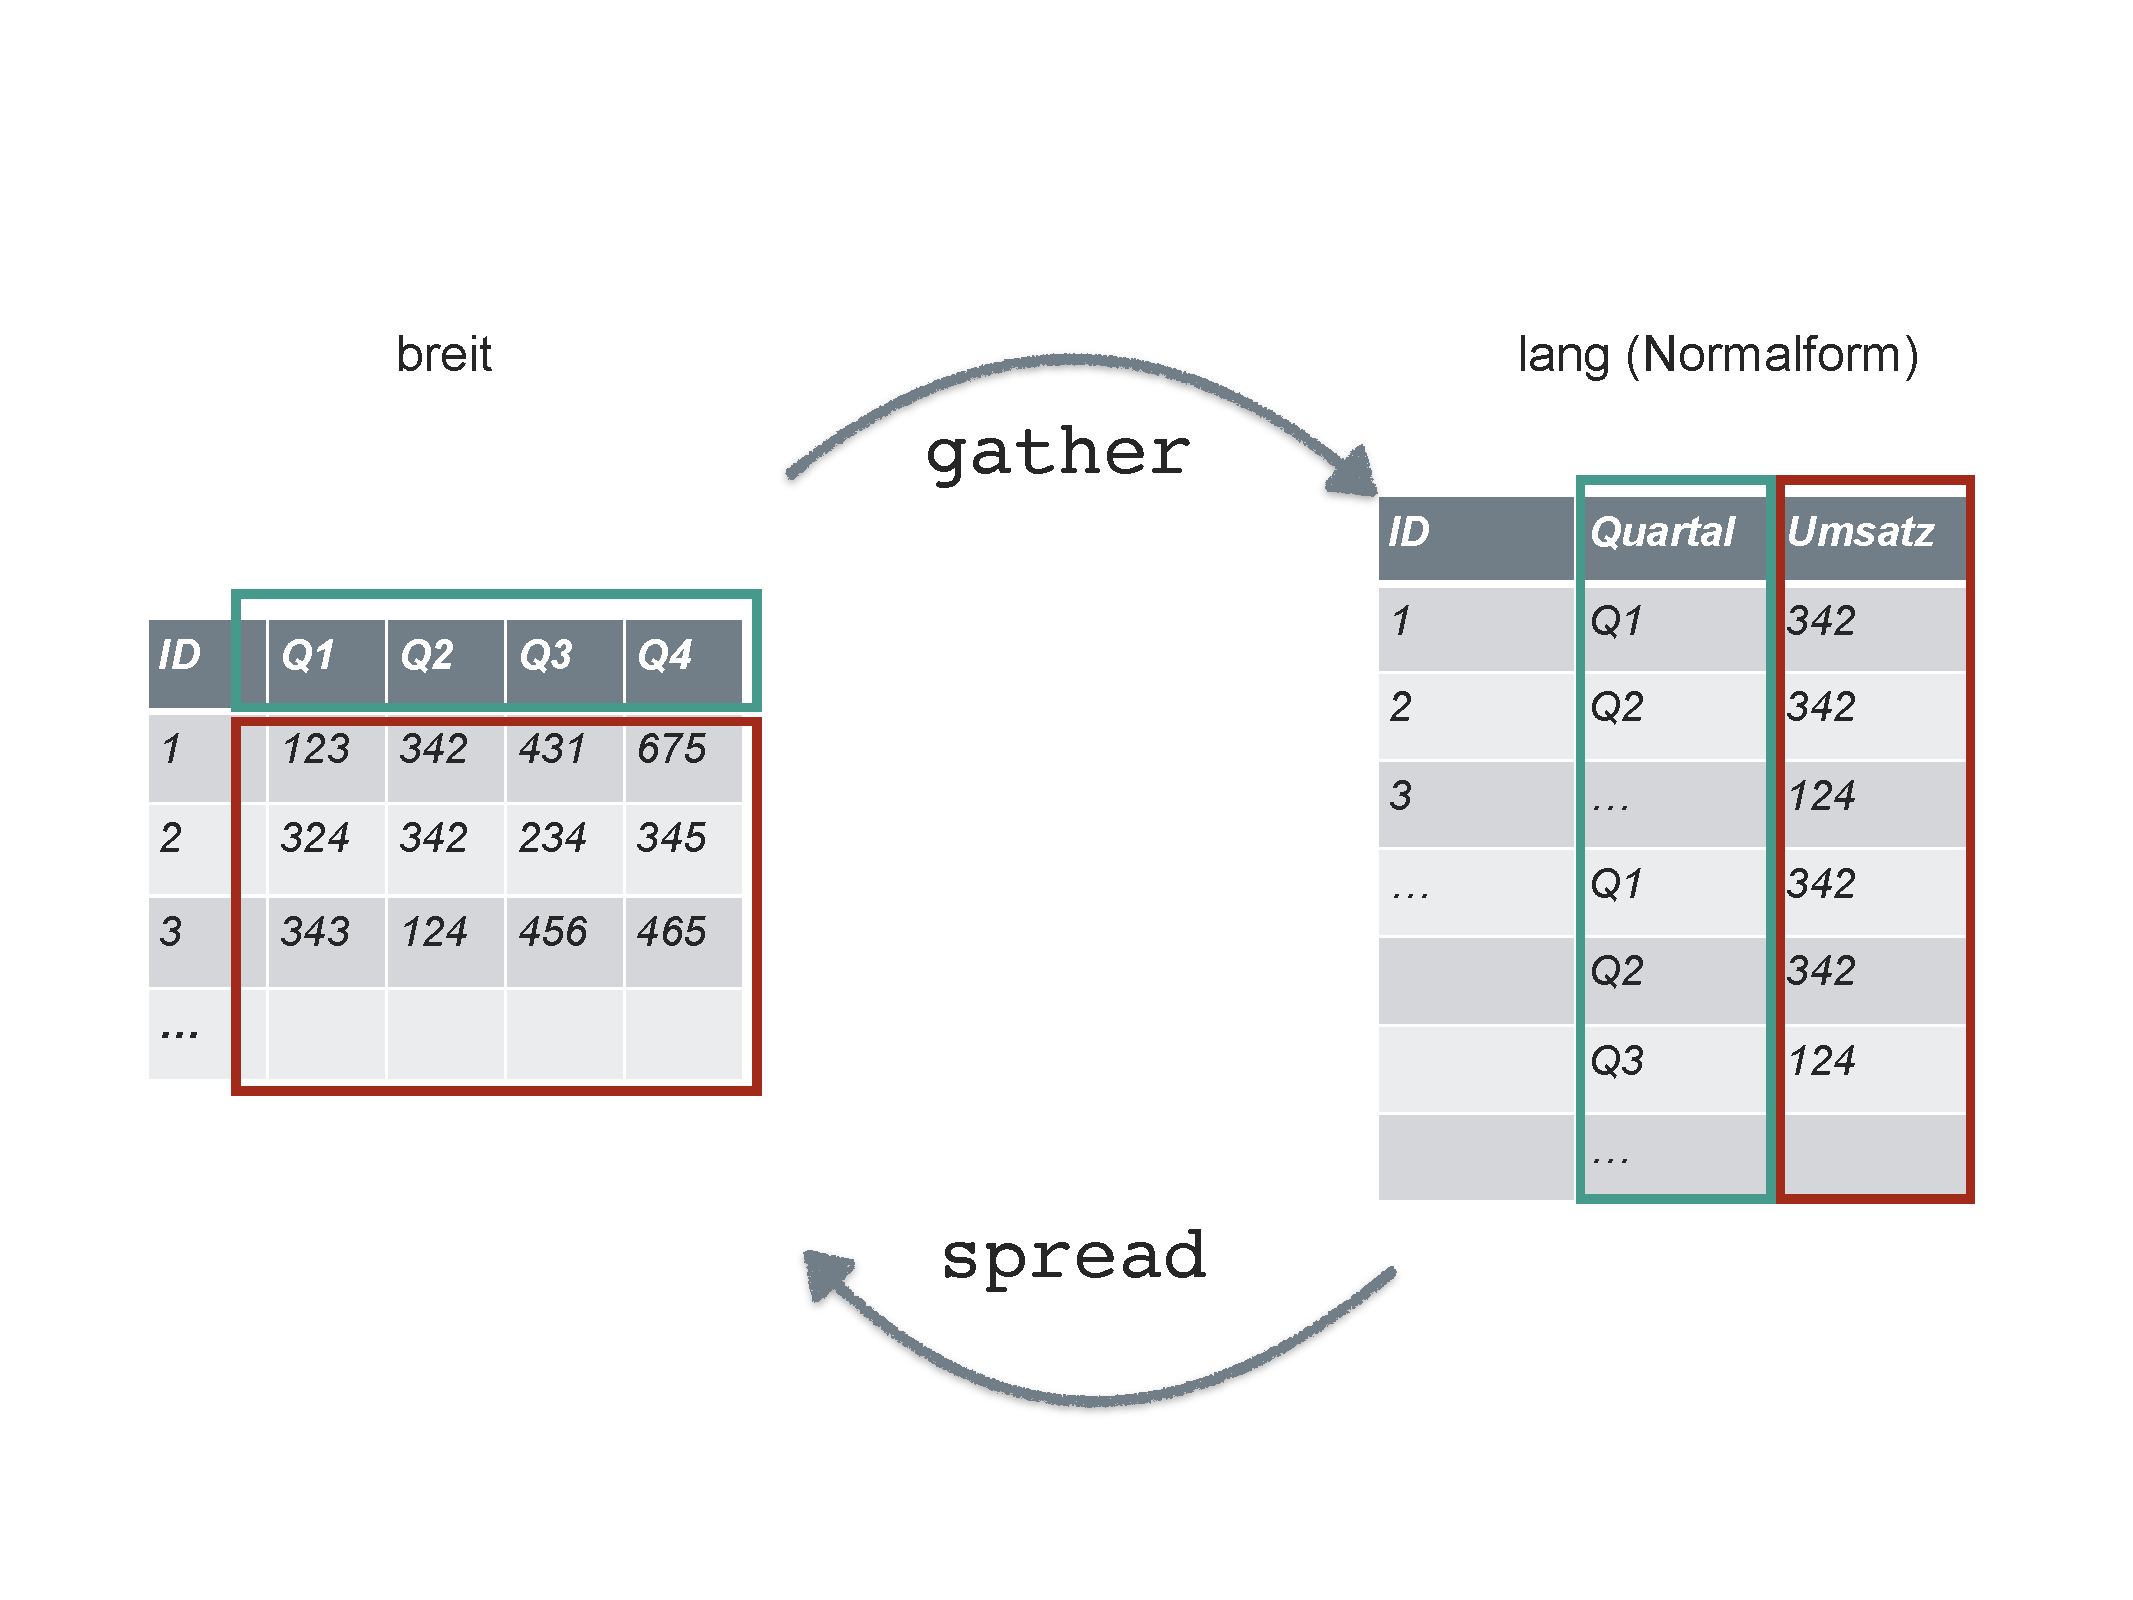
\includegraphics[width=0.7\linewidth]{images/tidy/gather_spread} 

}

\caption{Mit 'gather' und 'spread' wechselt man von der breiten Form zur langen Form}\label{fig:gather-spread}
\end{figure}

Warum ist es wichtig, von der ``breiten'' (links in Abb.
\ref{fig:gather-spread}) zur ``langen'' oder ``Normalform'' (rechts in
Abb. \ref{fig:gather-spread}) zu wechseln. Ganz einfach: viele Befehle
(allgemeiner: Tätigkeiten) verlangen die Normalform; hin und wieder sind
aber die Tabellen von ihrem Schöpfer in breiter Form geschaffen worden.
Zum Beispiel erwartet \texttt{ggplot2} - und viele andere
Diagrammbefehle - dass man \emph{einer} Achse \emph{eine} Spalte
(Variable) zuweist, z.B. die Variable ``Umsatz'' auf die Y-Achse. Der
X-Achse könnten wir dann z.B. die Variable ``Quartal'' packen (s. Abb.
\ref{fig:bsp-abb}).

\begin{figure}

{\centering 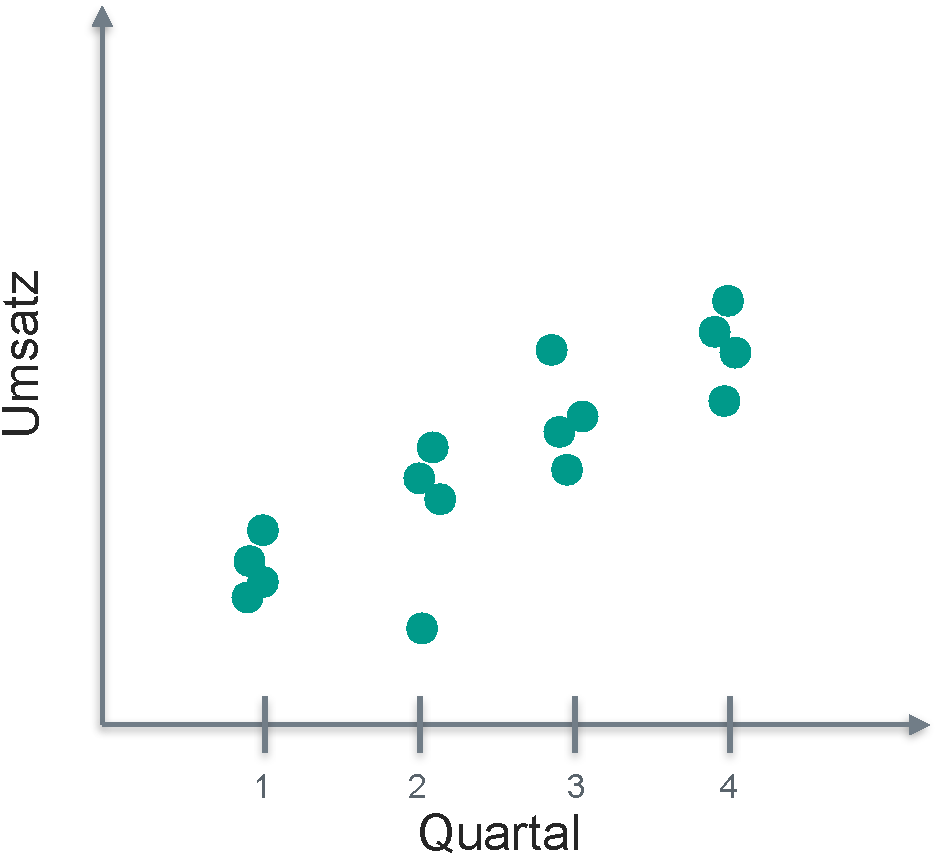
\includegraphics[width=0.7\linewidth]{images/tidy/bsp_diagramm-crop} 

}

\caption{Ein Beispiel für eine Abbildung zu einer Normalform-Tabelle}\label{fig:bsp-abb}
\end{figure}

Um von der breiten Form zur langen Form zu kommen, kann man den Befehl
\texttt{tidyr::gather} nehmen. Von der langen Form zur breiten From gibt
es \texttt{tidyr::spread}. Also etwa:

\begin{verbatim}
df_lang <- gather(df_breit, key = "Quartal", value = "Umsatz")

df_breit <- spread(df_lang, Quartal, Umsatz)
\end{verbatim}

Dabei baut \texttt{gather} den Dataframe so um, dass nur zwei Spalten
übrig bleiben (s. Abb. \ref{fig:gather-spread}). Eine Spalte nur
\emph{Spaltennamen} (``Q1'', ``Q2'', \ldots{}) enthält; diese Spalte
nennt \texttt{gather} im Standard \texttt{key}. Die zweite Spalte
enthält die Werte (z.B. Umsätze), die vormals über mehrere Spalten
verstreut waren. Diese Spalte heißt per Default \texttt{value}. Im
Beispiel oben macht die Spalte \texttt{ID} bei dem Spiel ``Aus vielen
Spalten werden zwei'' nicht mit. Möchte man eine Spalte aussparen, so
schreibt man das bei \texttt{gather} so:

\begin{verbatim}
df_lang <- gather(df_breit, key = "Quartal", value = "Umsatz", -ID)
\end{verbatim}

In Kapitel \ref{case-movies} werden wir dazu ein Fallstudie einüben.

\section{Textkodierung}\label{textkodierung}

Öffnet man eine Textdatei mit einem Texteditor seiner Wahl, so sieht
man\ldots{} Text und sonst nichts, also keine Formatierung etc. Eine
Textdatei besteht aus Text und sonst nichts (daher der Name\ldots{}).
Auch eine R-Skript-Datei (\texttt{Coole\_Syntax.R}) ist eine Textdatei.
Technisch gesprochen werden nur die Textzeichen gespeichert, sonst
nichts; im Gegensatz dazu speichert eine Word-Datei noch mehr, z.B.
Formatierung. Ein bestimmtes Zeichen wie ``A'' bekommt einen bestimmten
Code wie ``41''. Mit etwas Glück weiß der Computer jetzt, dass er das
Zeichen ``41'' auf den Bildschirm ausgeben soll. Es stellt sich jetzt
die Frage, welche Code-Tabelle der Computer nutzt? Welchem Code wird
``A'' (bzw. ein beliebiges Zeichen) zugeordnet? Mehrere solcher
Kodierungstafeln existieren. Die gebräuchlichste im Internet heißt
\emph{UTF-8}\footnote{\url{https://de.wikipedia.org/wiki/UTF-8}}. Leider
benutzen unterschiedliche Betriebssysteme unterschiedliche
Kodierungstafeln, was zu Verwirrung führt. Ich empfehle, ihre
Textdateien als UTF-8 zu kodieren. RStudio fragt sie, wie eine Textdatei
kodiert werden soll. Sie können auch unter
\texttt{File\ \textgreater{}\ Save\ with\ Encoding...} die Kodierung
einer Textdatei festlegen.

\begin{quote}
Speichern Sie R-Textdateien wie Skripte stets mit UTF-8-Kodierung ab.
\end{quote}

\subsection{Daten exportieren}\label{daten-exportieren}

Wie bekommt man seine Daten wieder aus R raus (``ich will zu Excel
zurück!'')?

Eine Möglichkeit bietet die Funktion \texttt{write.csv}; sie schreibt
eine CSV-Datei:

\begin{verbatim}
write.csv(name_der_tabelle, "Dateiname.csv")
\end{verbatim}

Mit \texttt{help(write.csv)} bekommt man mehr Hinweise dazu. Beachten
Sie, dass immer in das aktuelle Arbeitsverzeichnis geschrieben wird.

\section{Befehlsübersicht}\label{befehlsubersicht-1}

Tabelle \ref{tab:befehle-tidy} stellt die Befehle dieses Kapitels dar.

\begin{verbatim}
#> Parsed with column specification:
#> cols(
#>   `Paket::Funktion` = col_character(),
#>   Beschreibung = col_character()
#> )
\end{verbatim}

\begin{table}

\caption{\label{tab:befehle-tidy}Befehle des Kapitels 'Daten einlesen'}
\centering
\begin{tabular}[t]{l|l}
\hline
Paket::Funktion & Beschreibung\\
\hline
read.csv & Liest eine CSV-Datei ein.\\
\hline
write.csv & Schreibt einen Dateframe in eine CSV-Datei.\\
\hline
tidyr::gather & Macht aus einem "breiten" Dataframe einen "langen".\\
\hline
tidyr::separate & "Zieht" Spalten auseinander.\\
\hline
\end{tabular}
\end{table}

\section[Aufgaben]{\texorpdfstring{Aufgaben\footnote{F, R, F, R, R, R,
  F, F}}{Aufgaben}}\label{aufgaben-2}

\BeginKnitrBlock{rmdexercises}
Richtig oder Falsch!?

\begin{enumerate}
\def\labelenumi{\arabic{enumi}.}
\tightlist
\item
  In CSV-Dateien dürfen Spalten \emph{nie} durch Komma getrennt sein.
\item
  RStudio bietet die Möglichkeit, CSV-Dateien per Klick zu importieren.
\item
  RStudio bietet \emph{nicht} die Möglichkeit, CSV-Dateien per Klick zu
  importieren.
\item
  ``Deutsche'' CSV-Dateien verwenden als Spalten-Trennzeichen einen
  Strichpunkt.
\item
  In einer Tabelle in Normalform stehen in jeder Zeile eine Beobachtung.
\item
  In einer Tabelle in Normalform stehen in jeder Spalte eine Variable.
\item
  R stellt fehlende Werte mit einem Fragezeichen \texttt{?} dar.
\item
  Um Excel-Dateien zu importieren, kann man den Befehl \texttt{read.csv}
  verwenden.
\end{enumerate}
\EndKnitrBlock{rmdexercises}

\section{Verweise}\label{verweise-1}

\begin{itemize}
\tightlist
\item
  \emph{R for Data Science} bietet umfangreiche Unterstützung zu diesem
  Thema (Wickham und Grolemund \protect\hyperlink{ref-r4ds}{2016}).
\end{itemize}

\chapter{Datenjudo}\label{datenjudo}

\begin{center}
\includegraphics[width=0.3\linewidth]{images/FOM} \end{center}

\begin{center}
\includegraphics[width=0.1\linewidth]{images/licence} \end{center}

\BeginKnitrBlock{rmdcaution}
Lernziele:

\begin{itemize}
\tightlist
\item
  Die zentralen Ideen der Datenanalye mit dplyr verstehen.
\item
  Typische Probleme der Datenanalyse schildern können.
\item
  Zentrale \texttt{dplyr}-Befehle anwenden können.
\item
  \texttt{dplyr}-Befehle kombinieren können.
\item
  Die Pfeife anwenden können.
\item
  Werte umkodieren und ``binnen'' können.
\end{itemize}
\EndKnitrBlock{rmdcaution}

\begin{figure}

{\centering 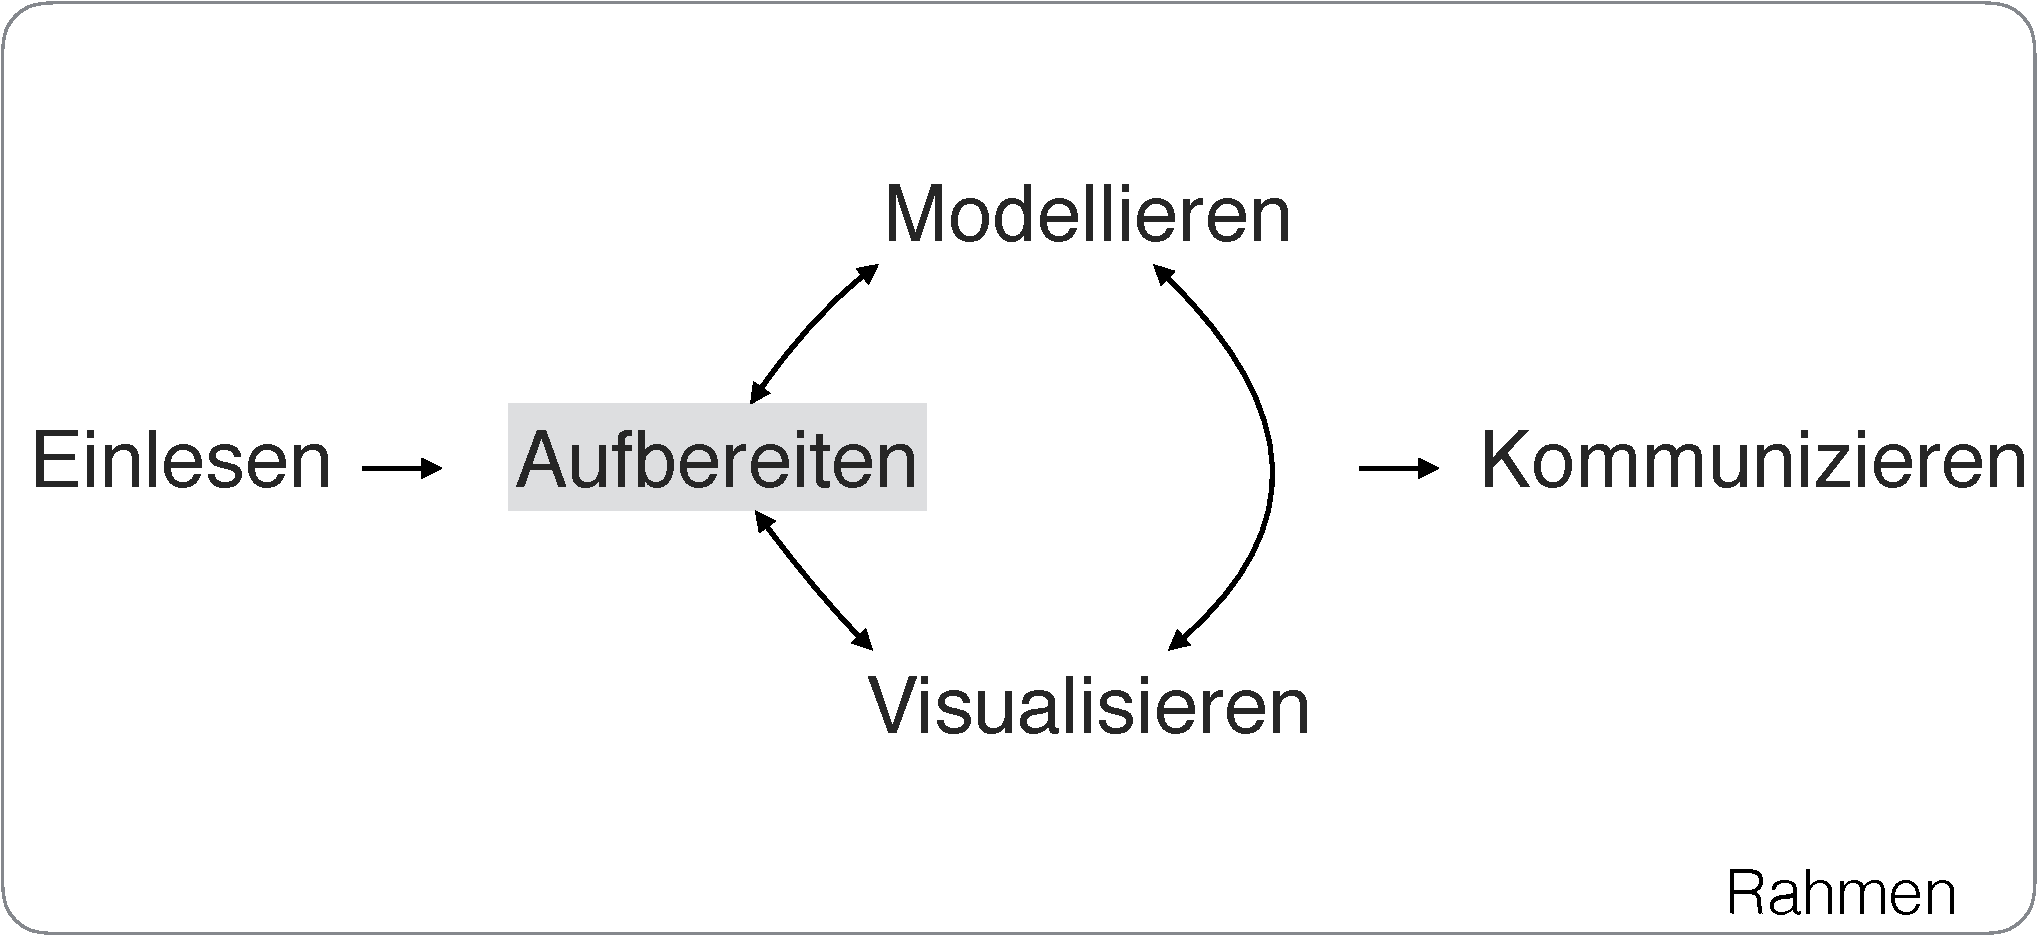
\includegraphics[width=0.7\linewidth]{images/Datenjudo/Aufbereiten} 

}

\caption{Daten aufbereiten}\label{fig:fig-datenjudo}
\end{figure}

In diesem Kapitel werden folgende Pakete benötigt:

\begin{Shaded}
\begin{Highlighting}[]
\KeywordTok{library}\NormalTok{(tidyverse)  }\CommentTok{# Datenjudo}
\KeywordTok{library}\NormalTok{(stringr)   }\CommentTok{# Texte bearbeiten}
\KeywordTok{library}\NormalTok{(car)  }\CommentTok{# für 'recode'}
\end{Highlighting}
\end{Shaded}

Das Paket \texttt{tidyverse} lädt \texttt{dplyr}, \texttt{ggplot2} und
weitere Pakete\footnote{für eine Liste s.
  \texttt{tidyverse\_packages(include\_self\ =\ TRUE)}}. Daher ist es
komfortabler, \texttt{tidyverse} zu laden, damit spart man sich
Tipparbeit. Die eigentliche Funktionalität, die wir in diesem Kapitel
nutzen, kommt aus dem Paket \texttt{dplyr}.

Mit \emph{Datenjudo}\index{Datenjudo} ist gemeint, die Daten für die
eigentliche Analyse ``aufzubereiten''. Unter
\emph{Aufbereiten}\index{Datenjudo} ist hier das Umformen, Prüfen,
Bereinigen, Gruppieren und Zusammenfassen von Daten gemeint. Die
deskriptive Statistik fällt unter die Rubrik Aufbereiten. Kurz gesagt:
Alles, wan tut, nachdem die Daten ``da'' sind und bevor man mit
anspruchsvoller(er) Modellierung beginnt.

Ist das Aufbereiten von Daten auch nicht statistisch anspruchsvoll, so
ist es trotzdem von großer Bedeutung und häufig recht zeitintensiv. Eine
Anekdote zur Relevanz der Datenaufbereitung, die (so will es die
Geschichte) mir an einer Bar nach einer einschlägigen Konferenz erzählt
wurde (daher keine Quellenangebe, Sie verstehen\ldots{}). Eine
Computerwissenschaftlerin aus den USA (deutschen Ursprungs) hatte einen
beeindruckenden ``Track Record'' an Siegen in Wettkämpfen der
Datenanalyse. Tatsächlich hatte sie keine besonderen, raffinierten
Modellierungstechniken eingesetzt; klassische Regression war ihre
Methode der Wahl. Bei einem Wettkampf, bei dem es darum ging, Krebsfälle
aus Krankendaten vorherzusagen (z.B. von Röntgenbildern) fand sie nach
langem Datenjudo heraus, dass in die ``ID-Variablen'' Information
gesickert war, die dort nicht hingehörte und die sie nutzen konnte für
überraschend (aus Sicht der Mitstreiter) gute Vorhersagen zu
Krebsfällen. Wie war das möglich? Die Daten stammten aus mehreren
Kliniken, jede Klinik verwendete ein anderes System, um IDs für
Patienten zu erstellen. Überall waren die IDs stark genug, um die
Anonymität der Patienten sicherzustellen, aber gleich wohl konnte man
(nach einigem Judo) unterscheiden, welche ID von welcher Klinik stammte.
Was das bringt? Einige Kliniken waren reine Screening-Zentren, die die
Normalbevölkerung versorgte. Dort sind wenig Krebsfälle zu erwarten.
Andere Kliniken jedoch waren Onkologie-Zentren für bereits bekannte
Patienten oder für Patienten mit besonderer Risikolage. Wenig
überraschen, dass man dann höhere Krebsraten vorhersagen kann.
Eigentlich ganz einfach; besondere Mathe steht hier (zumindest in dieser
Geschichte) nicht dahinter. Und, wenn man den Trick kennt, ganz einfach.
Aber wie so oft ist es nicht leicht, den Trick zu finden. Sorgfältiges
Datenjudo hat hier den Schlüssel zum Erfolg gebracht.

\section{Typische Probleme}\label{typische-probleme}

Bevor man seine Statistik-Trickkiste so richtig schön aufmachen kann,
muss man die Daten häufig erst noch in Form bringen. Das ist nicht
schwierig in dem Sinne, dass es um komplizierte Mathe ginge. Allerdings
braucht es mitunter recht viel Zeit und ein paar (oder viele)
handwerkliche Tricks sind hilfreich. Hier soll das folgende Kapitel
helfen.

Typische Probleme, die immer wieder auftreten, sind:

\begin{itemize}
\tightlist
\item
  \emph{Fehlende Werte}: Irgend jemand hat auf eine meiner schönen
  Fragen in der Umfrage nicht geantwortet!
\item
  \emph{Unerwartete Daten}: Auf die Frage, wie viele Facebook-Freunde er
  oder sie habe, schrieb die Person ``I like you a lot''. Was tun???
\item
  \emph{Daten müssen umgeformt werden}: Für jede der beiden Gruppen
  seiner Studie hat Joachim einen Google-Forms-Fragebogen aufgesetzt.
  Jetzt hat er zwei Tabellen, die er ``verheiraten'' möchte. Geht das?
\item
  \emph{Neue Variablen (Spalten) berechnen}: Ein Student fragt nach der
  Anzahl der richtigen Aufgaben in der Statistik-Probeklausur. Wir
  wollen helfen und im entsprechenden Datensatz eine Spalte erzeugen, in
  der pro Person die Anzahl der richtig beantworteten Fragen steht.
\end{itemize}

\section{\texorpdfstring{Daten aufbereiten mit
\texttt{dplyr}}{Daten aufbereiten mit dplyr}}\label{daten-aufbereiten-mit-dplyr}

Willkommen in der Welt von \texttt{dyplr}! \texttt{dplyr} hat seinen
Namen, weil es sich ausschließlich um \emph{D}ataframes bemüht; es
erwartet einen Dataframe als Eingabe und gibt einen Dataframe zurück
(zumindest bei den meisten Befehlen).

\subsection{\texorpdfstring{Die zwei Prinzipien von
\texttt{dplyr}}{Die zwei Prinzipien von dplyr}}\label{die-zwei-prinzipien-von-dplyr}

Es gibt viele Möglichkeiten, Daten mit R aufzubereiten;
\texttt{dplyr}\footnote{\url{https://cran.r-project.org/web/packages/dplyr/index.html}}
ist ein populäres Paket dafür. \texttt{dplyr} basiert auf zwei Ideen:

\begin{enumerate}
\def\labelenumi{\arabic{enumi}.}
\tightlist
\item
  \emph{Lego-Prinzip} Komplexe Datenanalysen in Bausteine zerlegen (vgl.
  Abb. \ref{fig:bausteine}).
\item
  \emph{Durchpfeifen}: Alle Operationen werden nur auf Dataframes
  angewendet; jede Operation erwartet einen Dataframe als Eingabe und
  gibt wieder einen Dataframe aus (vgl. Abb.
  \ref{fig:durchpfeifen-allgemein}).
\end{enumerate}

Das \emph{erste Prinzip} von \texttt{dplyr} ist, dass es nur ein paar
\emph{wenige Grundbausteine} geben sollte, die sich gut kombinieren
lassen. Sprich: Wenige grundlegende Funktionen mit eng umgrenzter
Funktionalität. Der Autor, Hadley Wickham, sprach einmal in einem Forum
(citation needed\ldots{}), dass diese Befehle wenig können, das Wenige
aber gut. Ein Nachteil dieser Konzeption kann sein, dass man recht viele
dieser Bausteine kombinieren muss, um zum gewünschten Ergebnis zu
kommen. Außerdem muss man die Logik des Baukastens gut verstanden habe -
die Lernkurve ist also erstmal steiler. Dafür ist man dann nicht darauf
angewiesen, dass es irgendwo ``Mrs Right'' gibt, die genau das kann, was
ich will. Außerdem braucht man sich auch nicht viele Funktionen merken.
Es reicht einen kleinen Satz an Funktionen zu kennen (die
praktischerweise konsistent in Syntax und Methodik sind). Diese
Bausteine sind typische Tätigkeiten im Umgang mit Daten; nichts
Überraschendes. Wir schauen wir uns diese Bausteine gleich näher an.

\begin{figure}

{\centering 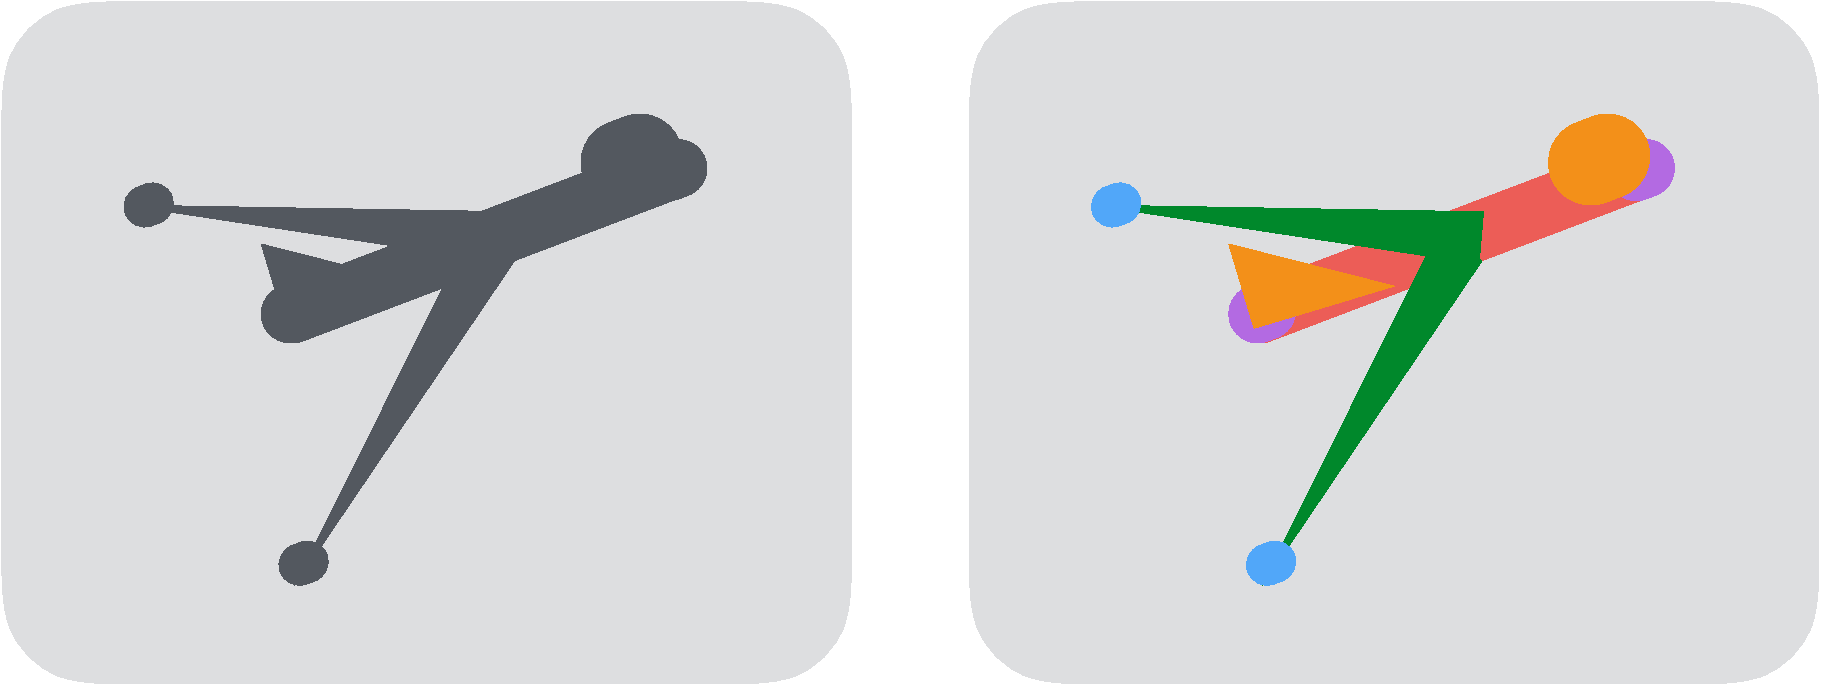
\includegraphics[width=0.7\linewidth]{images/Datenjudo/Bausteine_dplyr_crop} 

}

\caption{Lego-Prinzip: Zerlege eine komplexe Struktur in einfache Bausteine}\label{fig:bausteine}
\end{figure}

Das \emph{zweite Prinzip} von \texttt{dplyr} ist es, einen Dataframe von
Operation zu Operation \emph{durchzureichen.} \texttt{dplyr} arbeitet
also \emph{nur} mit Dataframes. Jeder Arbeitsschritt bei \texttt{dplyr}
erwartet einen Dataframe als Eingabe und gibt im Gegenzug wieder einen
Dataframe aus.

\begin{figure}

{\centering 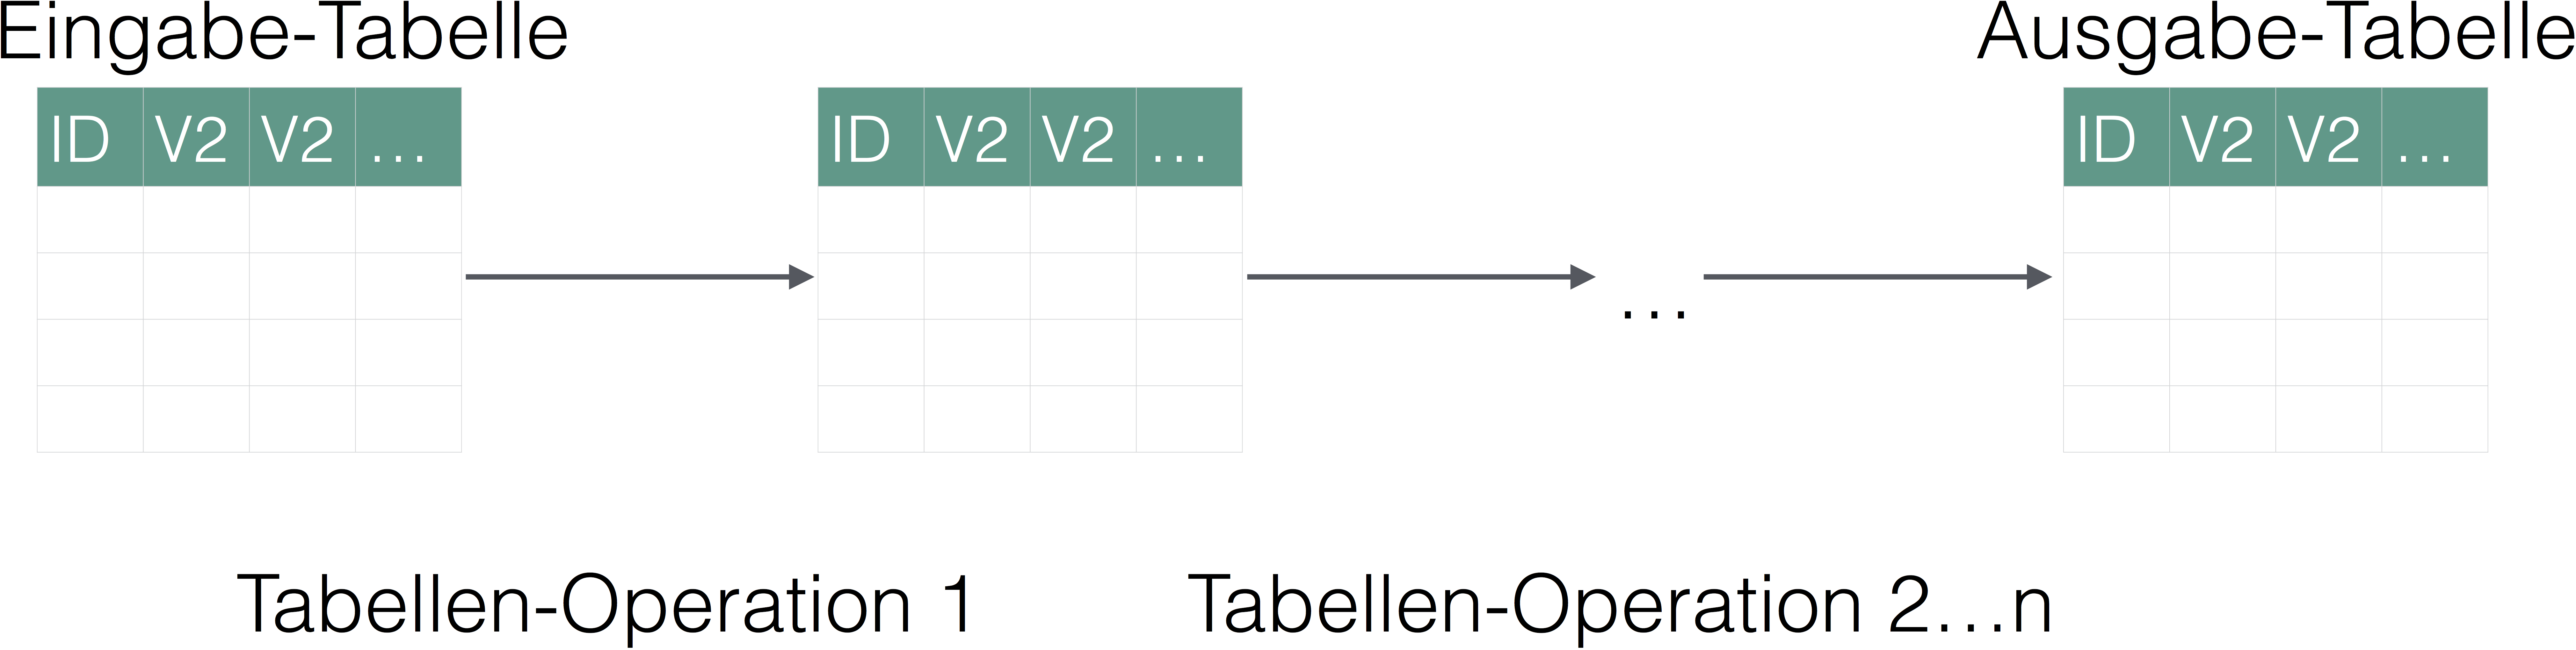
\includegraphics[width=0.7\linewidth]{images/Datenjudo/durchpfeifen_allgemein_crop} 

}

\caption{Durchpfeifen: Ein Dataframe wird von Operation zu Operation weitergereicht}\label{fig:durchpfeifen-allgemein}
\end{figure}

Werfen wir einen Blick auf ein paar typische Bausteine von
\texttt{dplyr}.

\section{\texorpdfstring{Zentrale Bausteine von
\texttt{dplyr}}{Zentrale Bausteine von dplyr}}\label{zentrale-bausteine-von-dplyr}

\subsection{\texorpdfstring{Zeilen filtern mit
\texttt{filter}}{Zeilen filtern mit filter}}\label{zeilen-filtern-mit-filter}

Häufig will man bestimmte Zeilen aus einer Tabelle filtern;
\texttt{filter}\index{dplyr::filter}. Zum Beispiel man arbeitet für die
Zigarettenindustrie und ist nur an den Rauchern interessiert (die im
Übrigen unser Gesundheitssystem retten (Krämer
\protect\hyperlink{ref-kraemer2011wir}{2011})), nicht an Nicht-Rauchern;
es sollen die nur Umsatzzahlen des letzten Quartals untersucht werden,
nicht die vorherigen Quartale; es sollen nur die Daten aus Labor X
(nicht Labor Y) ausgewertet werden etc.

Abb. \ref{fig:fig-filter} zeigt ein Sinnbild für \texttt{filter}.

\begin{figure}

{\centering 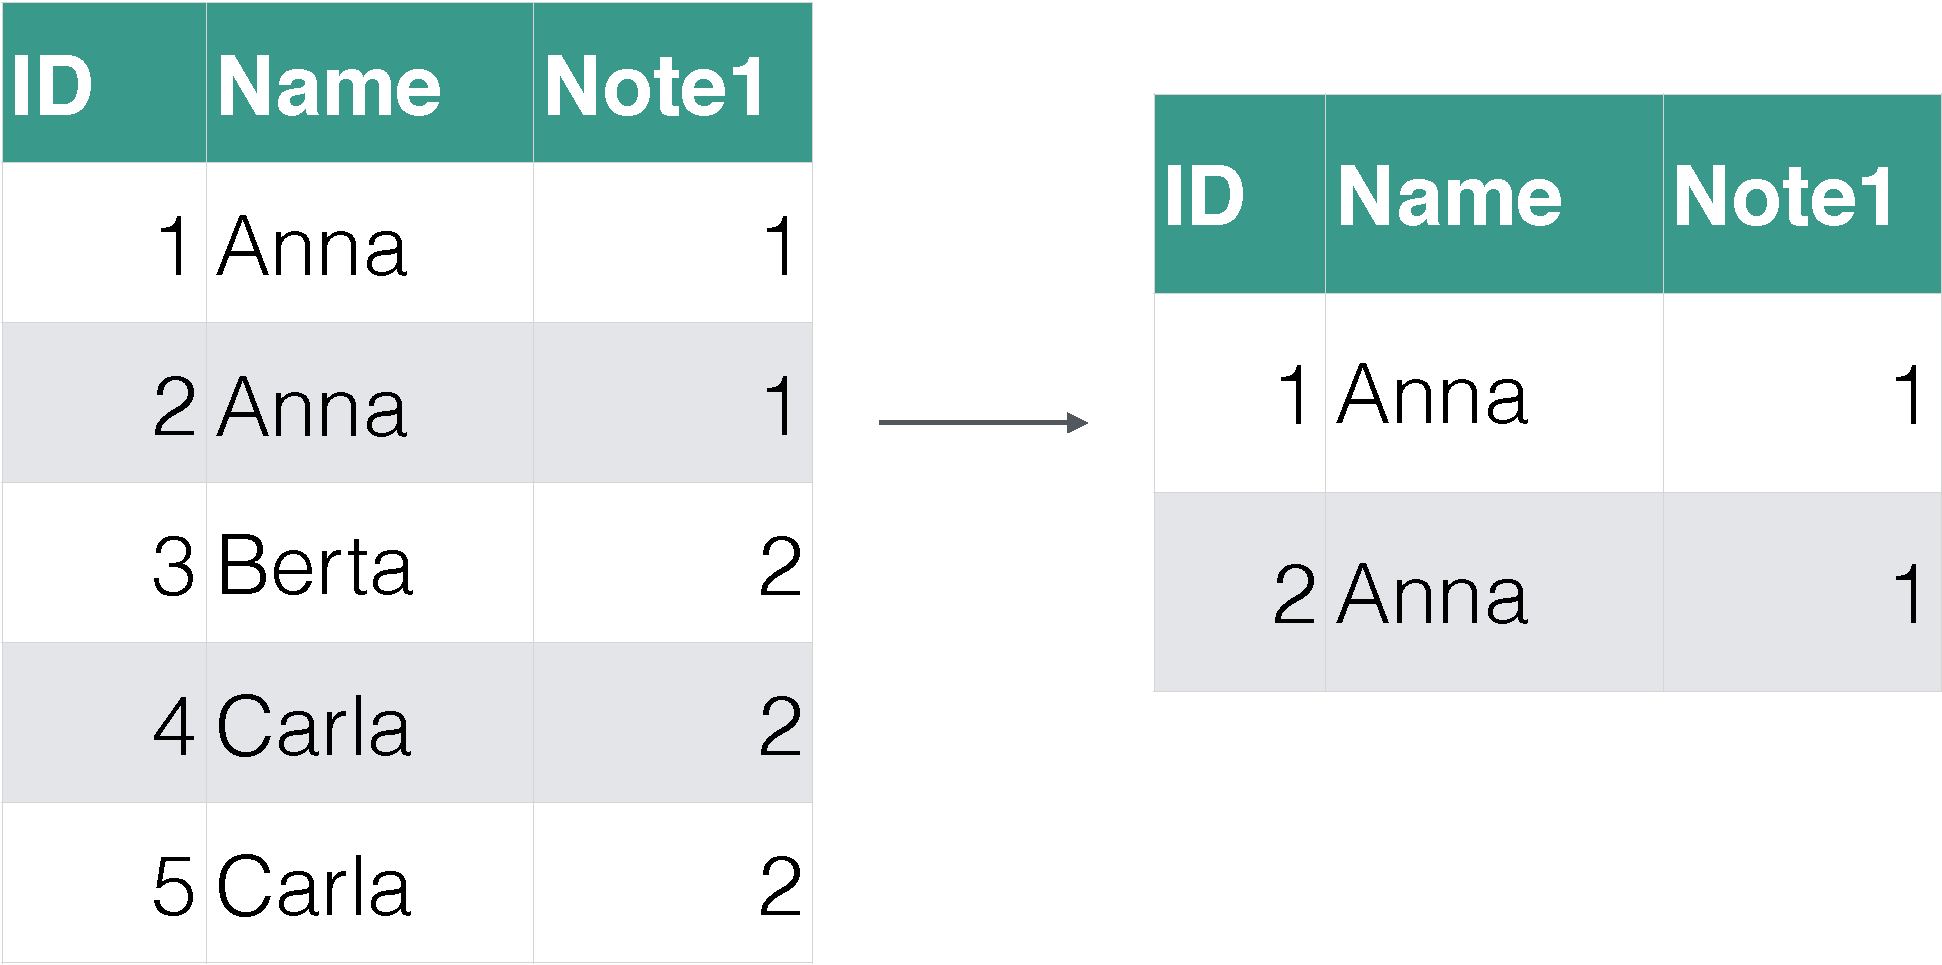
\includegraphics[width=0.7\linewidth]{images/Datenjudo/filter} 

}

\caption{Zeilen filtern}\label{fig:fig-filter}
\end{figure}

Merke:

\begin{quote}
Die Funktion \texttt{filter} filtert Zeilen aus einem Dataframe.
\end{quote}

Schauen wir uns einige Beispiel an; zuerst die Daten laden nicht
vergessen. Achtung: ``Wohnen'' die Daten in einem Paket, muss dieses
Paket installiert sein, damit man auf die Daten zugreifen kann.

\begin{Shaded}
\begin{Highlighting}[]
\KeywordTok{data}\NormalTok{(profiles, }\DataTypeTok{package =} \StringTok{"okcupiddata"}\NormalTok{)  }\CommentTok{# Das Paket muss installiert sein}
\end{Highlighting}
\end{Shaded}

\begin{Shaded}
\begin{Highlighting}[]
\NormalTok{df_frauen <-}\StringTok{ }\KeywordTok{filter}\NormalTok{(profiles, sex ==}\StringTok{ "f"}\NormalTok{)  }\CommentTok{# nur die Frauen}
\NormalTok{df_alt <-}\StringTok{ }\KeywordTok{filter}\NormalTok{(profiles, age >}\StringTok{ }\DecValTok{70}\NormalTok{)  }\CommentTok{# nur die alten Menschen}
\NormalTok{df_alte_frauen <-}\StringTok{ }\KeywordTok{filter}\NormalTok{(profiles, age >}\StringTok{ }\DecValTok{70}\NormalTok{, sex ==}\StringTok{ "f"}\NormalTok{) }
\CommentTok{# nur die alten Frauen, d.h. UND-Verknüpfung}

\NormalTok{df_nosmoke_nodrinks <-}\StringTok{ }\KeywordTok{filter}\NormalTok{(profiles, smokes ==}\StringTok{ "no"} \NormalTok{|}\StringTok{ }\NormalTok{drinks ==}\StringTok{ "not at all"}\NormalTok{) }
\CommentTok{# liefert alle Personen, die Nicht-Raucher *oder* Nicht-Trinker sind}
\end{Highlighting}
\end{Shaded}

Gar nicht so schwer, oder? Allgemeiner gesprochen werden diejenigen
Zeilen gefiltert (also behalten bzw. zurückgeliefert), für die das
Filterkriterium \texttt{TRUE} ist.

\BeginKnitrBlock{rmdcaution}
Manche Befehle wie \texttt{filter} haben einen Allerweltsnamen; gut
möglich, dass ein Befehl mit gleichem Namen in einem anderen (geladenen)
Paket existiert. Das kann dann zu Verwirrungen führen - und kryptischen
Fehlern. Im Zweifel den Namen des richtigen Pakets ergänzen, und zwar
zum Beispiel so: \texttt{dplyr::filter(...)}.
\EndKnitrBlock{rmdcaution}

\subsubsection[Aufgaben]{\texorpdfstring{Aufgaben\footnote{F, R, F, F, R}}{Aufgaben}}\label{aufgaben-3}

\BeginKnitrBlock{rmdexercises}
Richtig oder Falsch!?

\begin{enumerate}
\def\labelenumi{\arabic{enumi}.}
\tightlist
\item
  \texttt{filter} filtert Spalten.
\item
  \texttt{filter} ist eine Funktion aus dem Paket \texttt{dplyr}.
\item
  \texttt{filter} erwartet als ersten Parameter das Filterkriterium.
\item
  \texttt{filter} lässt nur ein Filterkriterium zu.
\item
  Möchte man aus dem Datensatz \texttt{profiles} (\texttt{okcupiddata})
  die Frauen filtern, so ist folgende Syntax korrekt:
  \texttt{filter(profiles,\ sex\ ==\ "f")}.
\end{enumerate}
\EndKnitrBlock{rmdexercises}

\subsubsection{\texorpdfstring{Vertiefung: Fortgeschrittene Beispiele
für
\texttt{filter}}{Vertiefung: Fortgeschrittene Beispiele für filter}}\label{vertiefung-fortgeschrittene-beispiele-fur-filter}

Einige fortgeschrittene Beispiele für \texttt{filter}:

Man kann alle Elemente (Zeilen) filtern, die zu einer Menge gehören und
zwar mit diesem Operator: \texttt{\%in\%}:

\begin{Shaded}
\begin{Highlighting}[]
\KeywordTok{filter}\NormalTok{(profiles, body_type %in%}\StringTok{ }\KeywordTok{c}\NormalTok{(}\StringTok{"a little extra"}\NormalTok{, }\StringTok{"average"}\NormalTok{))}
\end{Highlighting}
\end{Shaded}

Besonders Textdaten laden zu einigen Extra-Überlegungen ein; sagen wir,
wir wollen alle Personen filtern, die Katzen bei den Haustieren
erwähnen. Es soll reichen, wenn \texttt{cat} ein Teil des Textes ist;
also \texttt{likes\ dogs\ and\ likes\ cats} wäre OK (soll gefiltert
werden). Dazu nutzen wir ein Paket zur Bearbeitung von Strings
(Textdaten):

\begin{Shaded}
\begin{Highlighting}[]

\KeywordTok{filter}\NormalTok{(profiles, }\KeywordTok{str_detect}\NormalTok{(pets, }\StringTok{"cats"}\NormalTok{))}
\end{Highlighting}
\end{Shaded}

Ein häufiger Fall ist, Zeilen \emph{ohne} fehlende Werte (\texttt{NA}s)
zu filtern. Das geht einfach:

\begin{Shaded}
\begin{Highlighting}[]
\NormalTok{profiles_keine_nas <-}\StringTok{ }\KeywordTok{na.omit}\NormalTok{(profiles)}
\end{Highlighting}
\end{Shaded}

Aber was ist, wenn wir nur bei bestimmten Spalten wegen fehlender Werte
besorgt sind? Sagen wir bei \texttt{income} und bei \texttt{sex}:

\begin{Shaded}
\begin{Highlighting}[]
\KeywordTok{filter}\NormalTok{(profiles, !}\KeywordTok{is.na}\NormalTok{(income) |}\StringTok{ }\NormalTok{!}\KeywordTok{is.na}\NormalTok{(sex))}
\end{Highlighting}
\end{Shaded}

Der horizontale Strich \texttt{\textbar{}} steht bei R für logisches
`oder'.

\subsection{\texorpdfstring{Spalten wählen mit
\texttt{select}}{Spalten wählen mit select}}\label{spalten-wahlen-mit-select}

Das Gegenstück zu \texttt{filter} ist
\texttt{select}\index{dplyr::select}; dieser Befehl liefert die
gewählten Spalten zurück. Das ist häufig praktisch, wenn der Datensatz
sehr ``breit'' ist, also viele Spalten enthält. Dann kann es
übersichtlicher sein, sich nur die relevanten auszuwählen. Abb.
\ref{fig:fig-select} zeigt Sinnbild für diesen Befehl:

\begin{figure}

{\centering 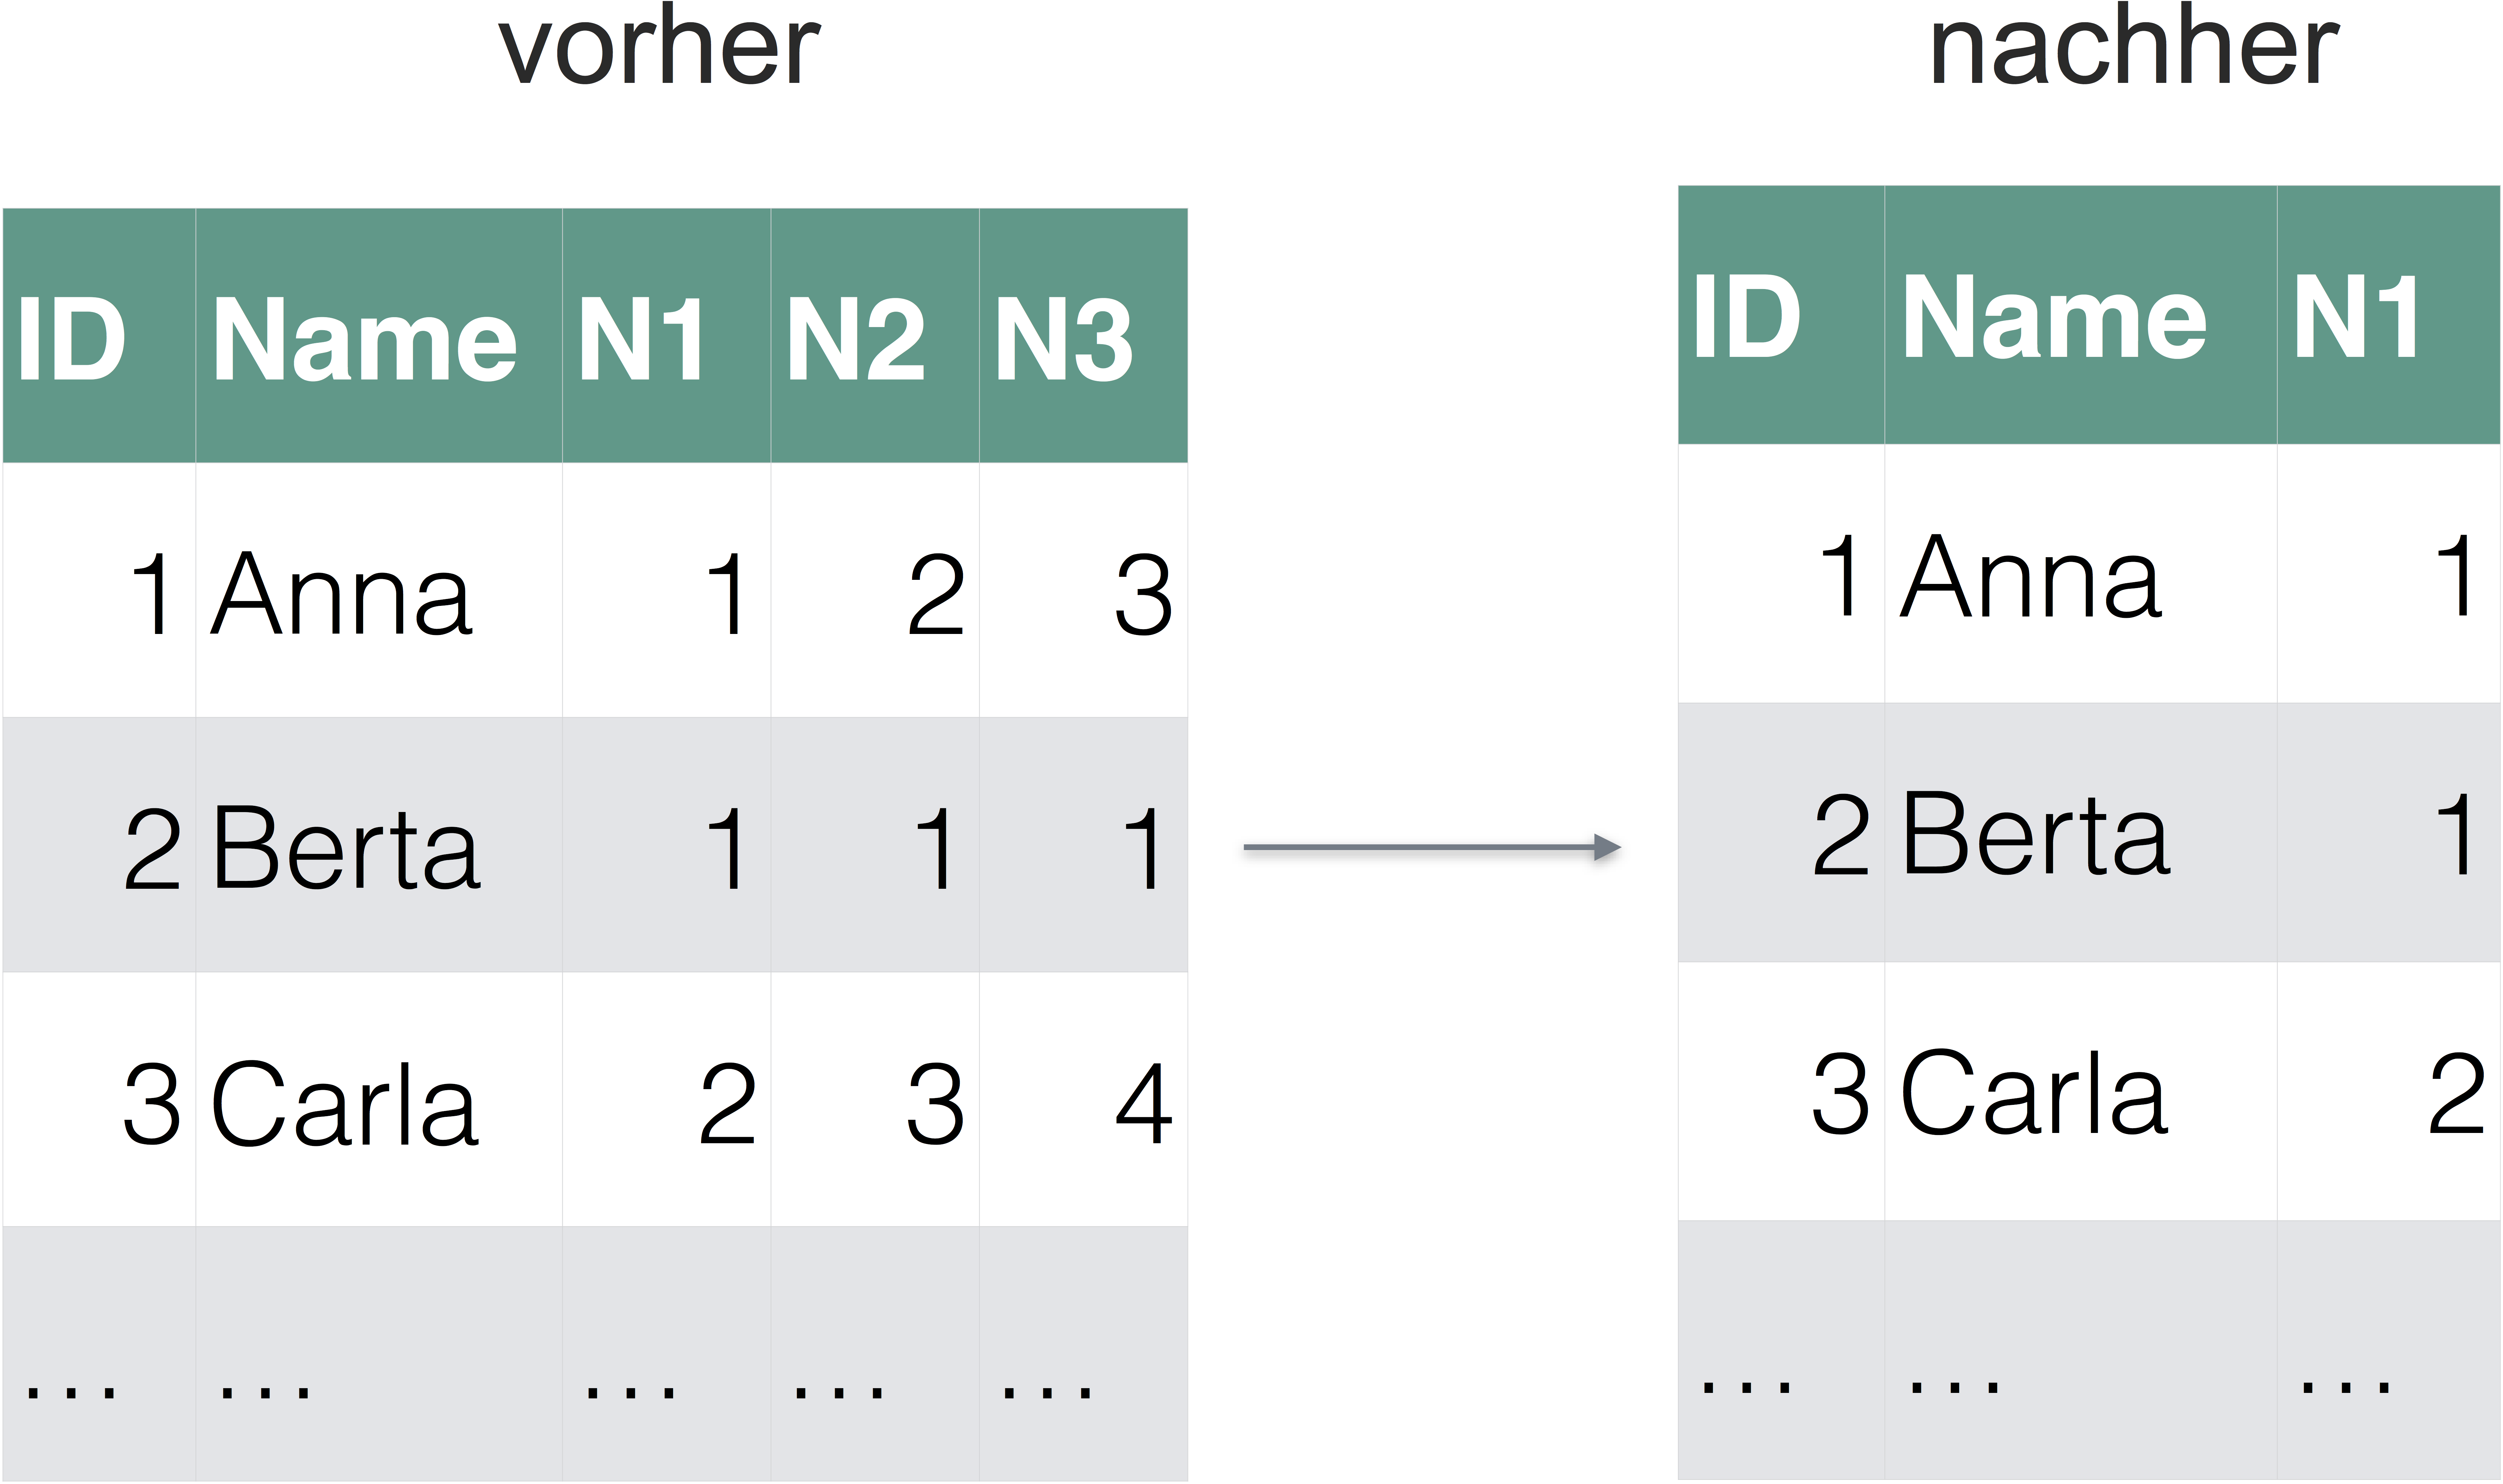
\includegraphics[width=0.7\linewidth]{images/Datenjudo/select} 

}

\caption{Spalten auswählen}\label{fig:fig-select}
\end{figure}

Merke:

\begin{quote}
Die Funktion select wählt Spalten aus einem Dataframe aus.
\end{quote}

Laden wir als ersten einen Datensatz.

\begin{Shaded}
\begin{Highlighting}[]
\NormalTok{stats_test <-}\StringTok{ }\KeywordTok{read.csv}\NormalTok{(}\StringTok{"data/test_inf_short.csv"}\NormalTok{)}
\end{Highlighting}
\end{Shaded}

Dieser Datensatz beinhaltet Daten zu einer Statistikklausur.

Beachten Sie, dass diese Syntax davon ausgeht, dass sich die Daten in
einem Unterordner mit dem Namen \texttt{data} befinden, welcher sich im
Arbeitsverzeichnis befindet\footnote{der angegebene Pfad ist also
  \emph{relativ} zum aktuellen Verzeichnis.}.

\begin{Shaded}
\begin{Highlighting}[]

\NormalTok{stats_test <-}\StringTok{ }\KeywordTok{read_csv}\NormalTok{(}\StringTok{"data/test_inf_short.csv"}\NormalTok{)}
\end{Highlighting}
\end{Shaded}

\begin{Shaded}
\begin{Highlighting}[]
\KeywordTok{select}\NormalTok{(stats_test, score)  }\CommentTok{# Spalte `score` auswählen}
\KeywordTok{select}\NormalTok{(stats_test, score, study_time)  }
\CommentTok{# Spalten `score` und `study_time` auswählen}

\KeywordTok{select}\NormalTok{(stats_test, score:study_time) }\CommentTok{# dito}
\KeywordTok{select}\NormalTok{(stats_test, }\DecValTok{5}\NormalTok{:}\DecValTok{6}\NormalTok{)  }\CommentTok{# Spalten 5 bis 6 auswählen}
\end{Highlighting}
\end{Shaded}

Tatsächlich ist der Befehl \texttt{select} sehr flexibel; es gibt viele
Möglichkeiten, Spalten auszuwählen. Im \texttt{dplyr}-Cheatsheet findet
sich ein guter Überblick dazu.

\subsubsection[Aufgaben]{\texorpdfstring{Aufgaben\footnote{F, F, R, R, F}}{Aufgaben}}\label{aufgaben-4}

\BeginKnitrBlock{rmdexercises}
Richtig oder Falsch!?

\begin{enumerate}
\def\labelenumi{\arabic{enumi}.}
\tightlist
\item
  \texttt{select} wählt \emph{Zeilen} aus.
\item
  \texttt{select} ist eine Funktion aus dem Paket \texttt{knitr}.
\item
  Möchte man zwei Spalten auswählen, so ist folgende Syntax prinzipiell
  korrekt: \texttt{select(df,\ spalte1,\ spalte2)}.
\item
  Möchte man Spalten 1 bis 10 auswählen, so ist folgende Syntax
  prinzipiell korrekt: `select(df, spalte1:spalte10)
\item
  Mit \texttt{select} können Spalten nur bei ihrem Namen, aber nicht bei
  ihrer Nummer aufgerufen werden.
\end{enumerate}
\EndKnitrBlock{rmdexercises}

\subsection{\texorpdfstring{Zeilen sortieren mit
\texttt{arrange}}{Zeilen sortieren mit arrange}}\label{zeilen-sortieren-mit-arrange}

Man kann zwei Arten des Umgangs mit R unterscheiden: Zum einen der
``interaktive Gebrauch'' und zum anderen ``richtiges Programmieren''. Im
interaktiven Gebrauch geht es uns darum, die Fragen zum aktuell
vorliegenden Datensatz (schnell) zu beantworten. Es geht nicht darum,
eine allgemeine Lösung zu entwickeln, die wir in die Welt verschicken
können und die dort ein bestimmtes Problem löst, ohne dass der
Entwickler (wir) dabei Hilfestellung geben muss. ``Richtige'' Software,
wie ein R-Paket oder Microsoft Powerpoint, muss diese Erwartung
erfüllen; ``richtiges Programmieren'' ist dazu vonnöten. Natürlich sind
in diesem Fall die Ansprüche an die Syntax (der ``Code'', hört sich
cooler an) viel höher. In dem Fall muss man alle Eventualitäten
voraussehen und sicherstellen, dass das Programm auch beim
merkwürdigsten Nutzer brav seinen Dienst tut. Wir haben hier, beim
interaktiven Gebrauch, niedrigere Ansprüche bzw. andere Ziele.

Beim interaktiven Gebrauch von R (oder beliebigen Analyseprogrammen) ist
das Sortieren von Zeilen eine recht häufige Tätigkeit. Typisches
Beispiel wäre der Lehrer, der eine Tabelle mit Noten hat und wissen
will, welche Schüler die schlechtesten oder die besten sind in einem
bestimmten Fach. Oder bei der Prüfung der Umsätze nach Filialen möchten
wir die umsatzstärksten sowie -schwächsten Niederlassungen kennen.

Ein R-Befehl hierzu ist \texttt{arrange}\index{dplyr::arrange}; einige
Beispiele zeigen die Funktionsweise am besten:

\begin{Shaded}
\begin{Highlighting}[]

\KeywordTok{arrange}\NormalTok{(stats_test, score) }\CommentTok{# liefert die *schlechtesten* Noten zuerst zurück}
\KeywordTok{arrange}\NormalTok{(stats_test, -score) }\CommentTok{# liefert die *besten* Noten zuerst zurück}
\KeywordTok{arrange}\NormalTok{(stats_test, interest, score)}
\end{Highlighting}
\end{Shaded}

\begin{verbatim}
#> # A tibble: 6 x 6
#>   row_number           date_time study_time self_eval interest score
#>        <int>               <chr>      <int>     <int>    <int> <int>
#> 1        234 23.01.2017 18:13:15          3         1        1    17
#> 2          4 06.01.2017 09:58:05          2         3        2    18
#> 3        131 19.01.2017 18:03:45          2         3        4    18
#> 4        142 19.01.2017 19:02:12          3         4        1    18
#> 5         35 12.01.2017 19:04:43          1         2        3    19
#> 6         71 15.01.2017 15:03:29          3         3        3    20
#> # A tibble: 6 x 6
#>   row_number           date_time study_time self_eval interest score
#>        <int>               <chr>      <int>     <int>    <int> <int>
#> 1          3 05.01.2017 23:33:47          5        10        6    40
#> 2          7 06.01.2017 14:25:49         NA        NA       NA    40
#> 3         29 12.01.2017 09:48:16          4        10        3    40
#> 4         41 13.01.2017 12:07:29          4        10        3    40
#> 5         58 14.01.2017 15:43:01          3         8        2    40
#> 6         83 16.01.2017 10:16:52         NA        NA       NA    40
#> # A tibble: 6 x 6
#>   row_number           date_time study_time self_eval interest score
#>        <int>               <chr>      <int>     <int>    <int> <int>
#> 1        234 23.01.2017 18:13:15          3         1        1    17
#> 2        142 19.01.2017 19:02:12          3         4        1    18
#> 3        221 23.01.2017 11:40:30          1         1        1    23
#> 4        230 23.01.2017 16:27:49          1         1        1    23
#> 5         92 17.01.2017 17:18:55          1         1        1    24
#> 6        107 18.01.2017 16:01:36          3         2        1    24
\end{verbatim}

Einige Anmerkungen. Die generelle Syntax lautet
\texttt{arrange(df,\ Spalte1,\ ...)}, wobei \texttt{df} den Dataframe
bezeichnet und \texttt{Spalte1} die erste zu sortierende Spalte; die
Punkte \texttt{...} geben an, dass man weitere Parameter übergeben kann.
Man kann sowohl numerische Spalten als auch Textspalten sortieren. Am
wichtigsten ist hier, dass man weitere Spalten übergeben kann. Dazu
gleich mehr.

Standardmäßig sortiert \texttt{arrange} \emph{aufsteigend} (weil kleine
Zahlen im Zahlenstrahl vor den großen Zahlen kommen). Möchte man diese
Reihenfolge umdrehen (große Werte zuert, d.h. \emph{absteigend}), so
kann man ein Minuszeichen vor den Namen der Spalte setzen.

Gibt man \emph{zwei oder mehr} Spalten an, so werden pro Wert von
\texttt{Spalte1} die Werte von \texttt{Spalte2} sortiert etc; man
betrachte den Output des Beispiels oben dazu.

Merke:

\begin{quote}
Die Funktion \texttt{arrange} sortiert die Zeilen eines Datafames.
\end{quote}

Ein Sinnbild zur Verdeutlichung (s. Abb. \ref{fig:fig-arrange}):

\begin{figure}

{\centering 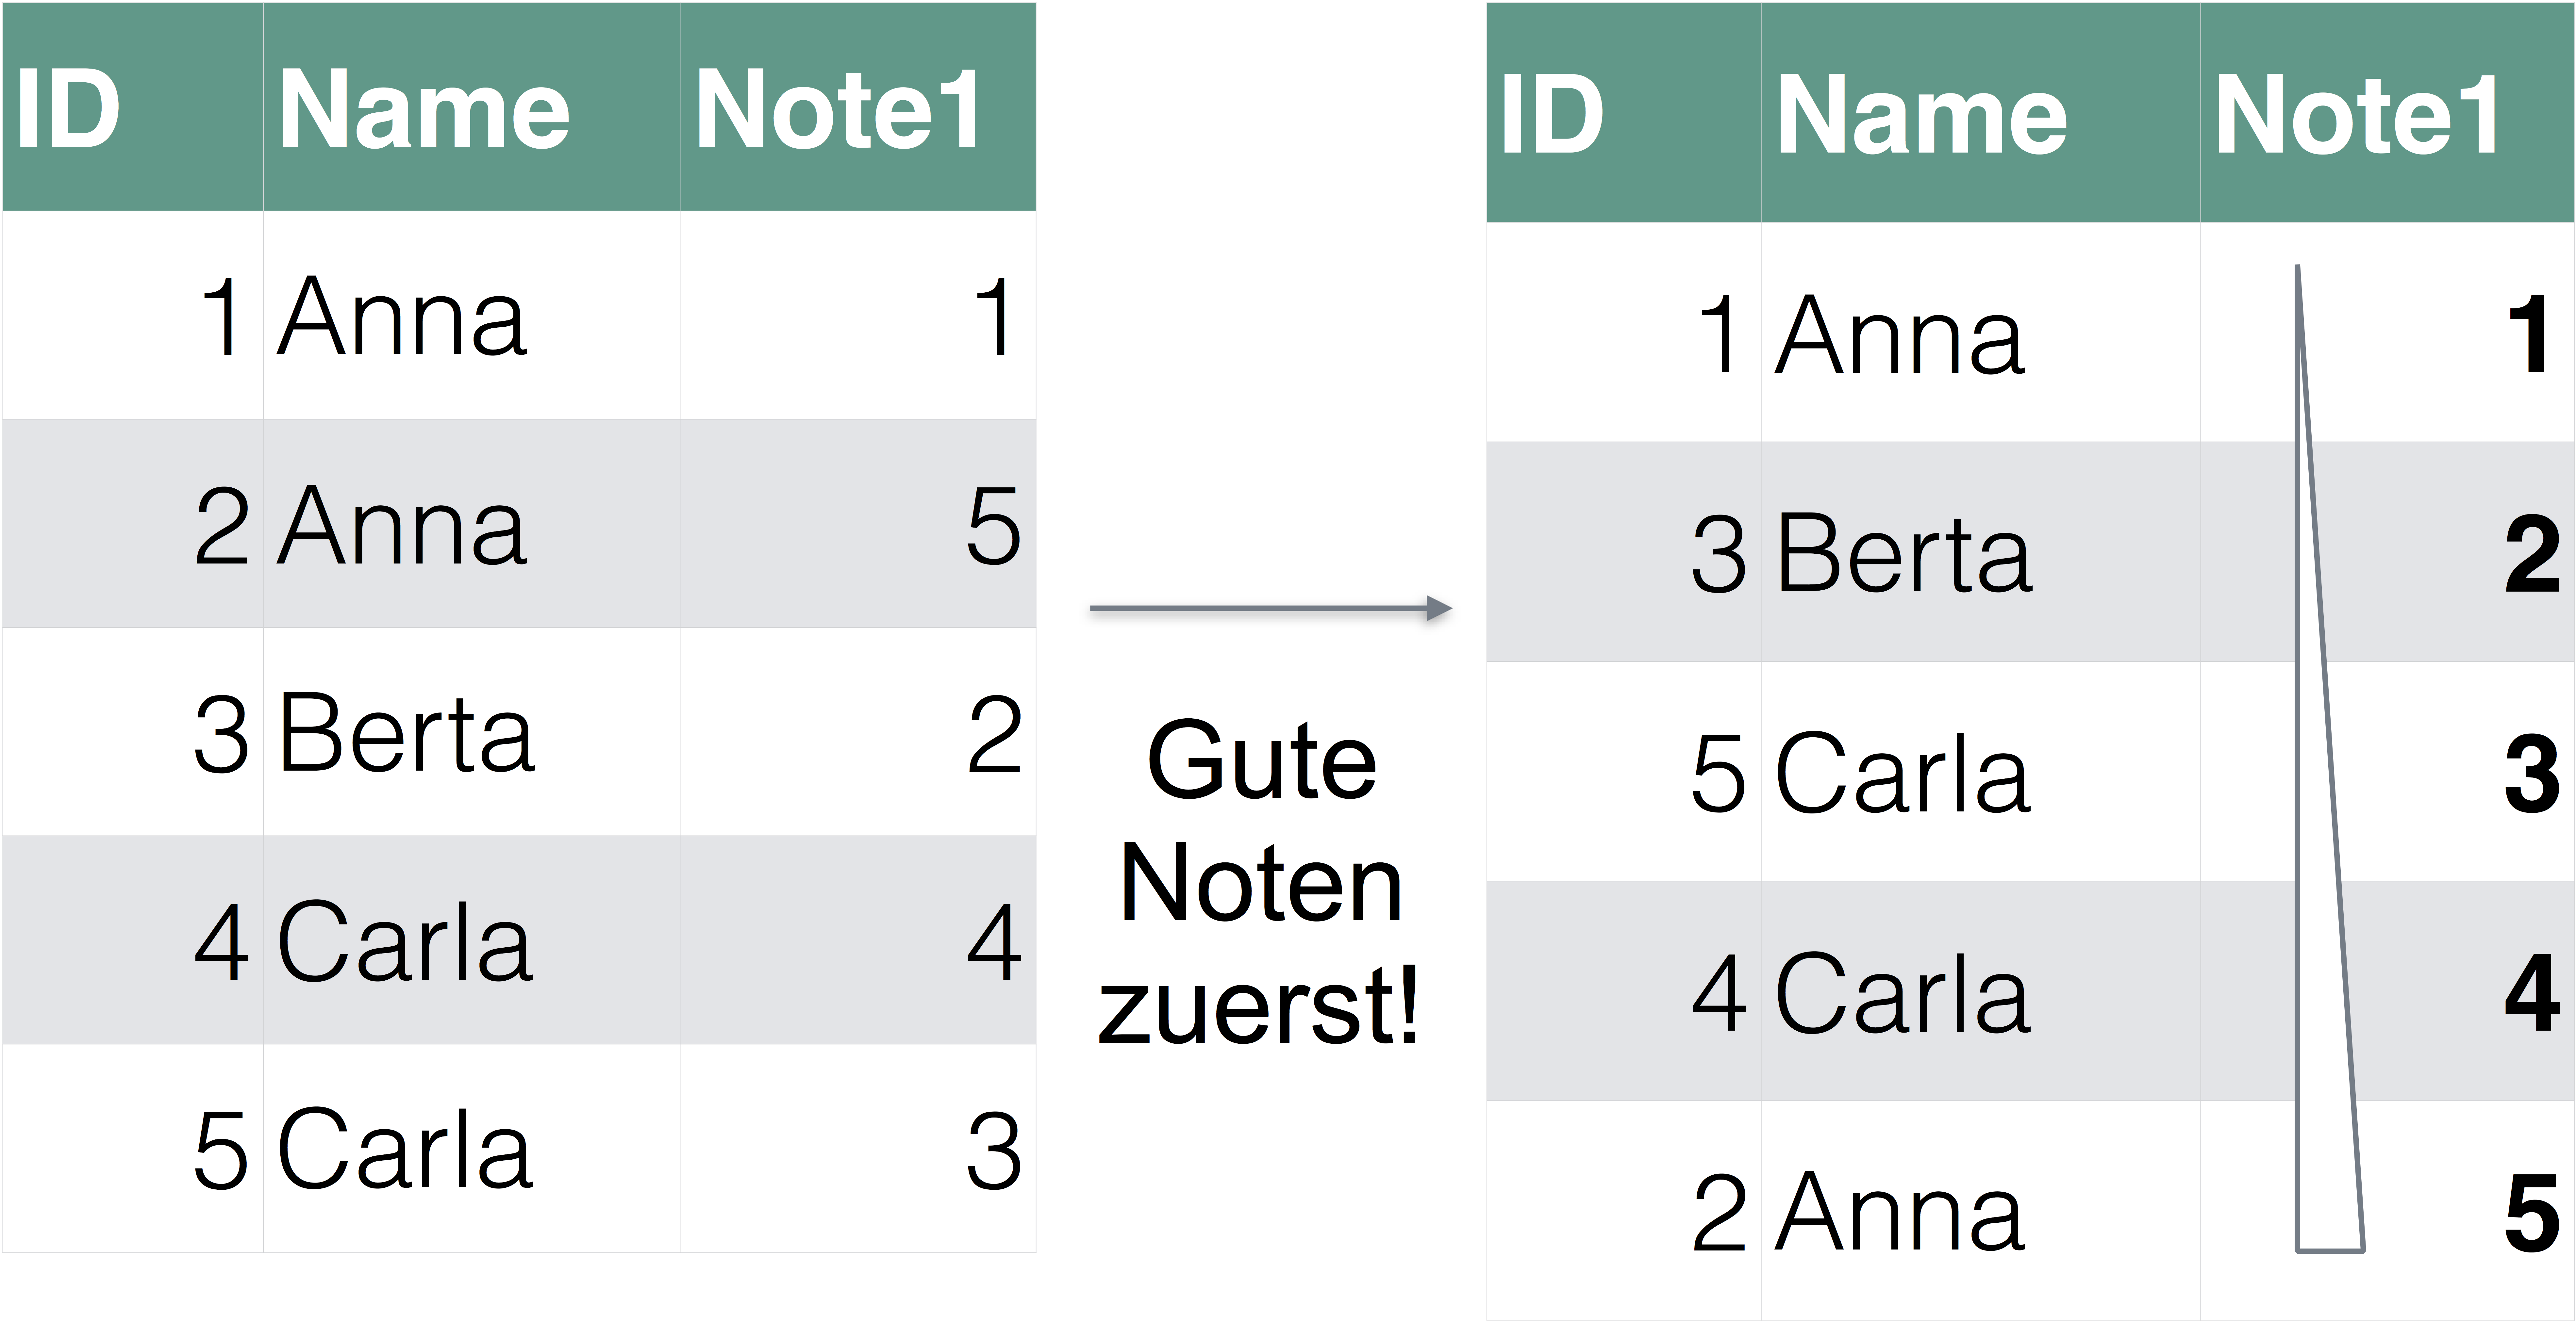
\includegraphics[width=0.7\linewidth]{images/Datenjudo/arrange-crop} 

}

\caption{Spalten sortieren}\label{fig:fig-arrange}
\end{figure}

Ein ähnliches Ergebnis erhält mit man \texttt{top\_n()}, welches die
\texttt{n} \emph{größten Elemente} widergibt:

\begin{Shaded}
\begin{Highlighting}[]

\KeywordTok{top_n}\NormalTok{(stats_test, }\DecValTok{3}\NormalTok{)}
\CommentTok{#> # A tibble: 18 x 6}
\CommentTok{#>    row_number           date_time study_time self_eval interest score}
\CommentTok{#>         <int>               <chr>      <int>     <int>    <int> <int>}
\CommentTok{#>  1          3 05.01.2017 23:33:47          5        10        6    40}
\CommentTok{#>  2          7 06.01.2017 14:25:49         NA        NA       NA    40}
\CommentTok{#>  3         29 12.01.2017 09:48:16          4        10        3    40}
\CommentTok{#>  4         41 13.01.2017 12:07:29          4        10        3    40}
\CommentTok{#>  5         58 14.01.2017 15:43:01          3         8        2    40}
\CommentTok{#>  6         83 16.01.2017 10:16:52         NA        NA       NA    40}
\CommentTok{#>  7        116 18.01.2017 23:07:32          4         8        5    40}
\CommentTok{#>  8        119 19.01.2017 09:05:01         NA        NA       NA    40}
\CommentTok{#>  9        132 19.01.2017 18:22:32         NA        NA       NA    40}
\CommentTok{#> 10        175 20.01.2017 23:03:36          5        10        5    40}
\CommentTok{#> 11        179 21.01.2017 07:40:05          5         9        1    40}
\CommentTok{#> 12        185 21.01.2017 15:01:26          4        10        5    40}
\CommentTok{#> 13        196 22.01.2017 13:38:56          4        10        5    40}
\CommentTok{#> 14        197 22.01.2017 14:55:17          4        10        5    40}
\CommentTok{#> 15        248 24.01.2017 16:29:45          2        10        2    40}
\CommentTok{#> 16        249 24.01.2017 17:19:54         NA        NA       NA    40}
\CommentTok{#> 17        257 25.01.2017 10:44:34          2         9        3    40}
\CommentTok{#> 18        306 27.01.2017 11:29:48          4         9        3    40}
\KeywordTok{top_n}\NormalTok{(stats_test, }\DecValTok{3}\NormalTok{, interest)}
\CommentTok{#> # A tibble: 9 x 6}
\CommentTok{#>   row_number           date_time study_time self_eval interest score}
\CommentTok{#>        <int>               <chr>      <int>     <int>    <int> <int>}
\CommentTok{#> 1          3 05.01.2017 23:33:47          5        10        6    40}
\CommentTok{#> 2          5 06.01.2017 14:13:08          4         8        6    34}
\CommentTok{#> 3         43 13.01.2017 14:14:16          4         8        6    36}
\CommentTok{#> 4         65 15.01.2017 12:41:27          3         6        6    22}
\CommentTok{#> 5        110 18.01.2017 18:53:02          5         8        6    37}
\CommentTok{#> 6        136 19.01.2017 18:22:57          3         1        6    39}
\CommentTok{#> 7        172 20.01.2017 20:42:46          5        10        6    34}
\CommentTok{#> 8        214 22.01.2017 21:57:36          2         6        6    31}
\CommentTok{#> 9        301 27.01.2017 08:17:59          4         8        6    33}
\end{Highlighting}
\end{Shaded}

Gibt man \emph{keine} Spalte an, so bezieht sich \texttt{top\_n} auf die
letzte Spalte im Datensatz.

Wenn sich aber, wie hier, mehrere Objekte, den größten Rang (Wert 40)
teilen, bekommen wir \emph{nicht} 3 Zeilen zurückgeliefert, sondern
entsprechend mehr. dplyr ``denkt'' sich: ``Ok, er will die drei besten
Werte; aber ersten 4 haben alle den gleichen Wert, wen sollte ich da
ausschließen? Am besten ich liefere alle zurück, die den gleichen Wert
habe, falls ich sonst zu wenig Objekte zurückliefern würde''.

\subsubsection[Aufgaben]{\texorpdfstring{Aufgaben\footnote{F, F, F, F, F}}{Aufgaben}}\label{aufgaben-5}

\BeginKnitrBlock{rmdexercises}
Richtig oder Falsch!?

\begin{enumerate}
\def\labelenumi{\arabic{enumi}.}
\tightlist
\item
  \texttt{arrange} arrangiert Spalten.
\item
  \texttt{arrange} sortiert im Standard absteigend.
\item
  \texttt{arrange} lässt nur ein Sortierkriterium zu.
\item
  \texttt{arrange} kann numerische Werte, aber nicht Zeichenketten
  sortieren.
\item
  \texttt{top\_n(5)} liefert immer fünf Werte zurück.
\end{enumerate}
\EndKnitrBlock{rmdexercises}

\subsection{\texorpdfstring{Datensatz gruppieren mit
\texttt{group\_by}}{Datensatz gruppieren mit group\_by}}\label{datensatz-gruppieren-mit-group_by}

Einen Datensatz zu gruppieren ist eine häufige Angelegenheit: Was ist
der mittlere Umsatz in Region X im Vergleich zu Region Y? Ist die
Reaktionszeit in der Experimentalgruppe kleiner als in der
Kontrollgruppe? Können Männer schneller ausparken als Frauen? Man sieht,
dass das Gruppieren v.a. in Verbindung mit Mittelwerten oder anderen
Zusammenfassungen sinnvol ist; dazu im nächsten Abschnitt mehr.

\begin{quote}
Gruppieren meint, einen Datensatz anhand einer diskreten Variablen (z.B.
Geschlecht) so aufzuteilen, dass Teil-Datensätze entstehen - pro Gruppe
ein Teil-Datensatz (z.B. ein Datensatz, in dem nur Männer enthalten sind
und einer, in dem nur Frauen enthalten sind).
\end{quote}

\begin{figure}

{\centering 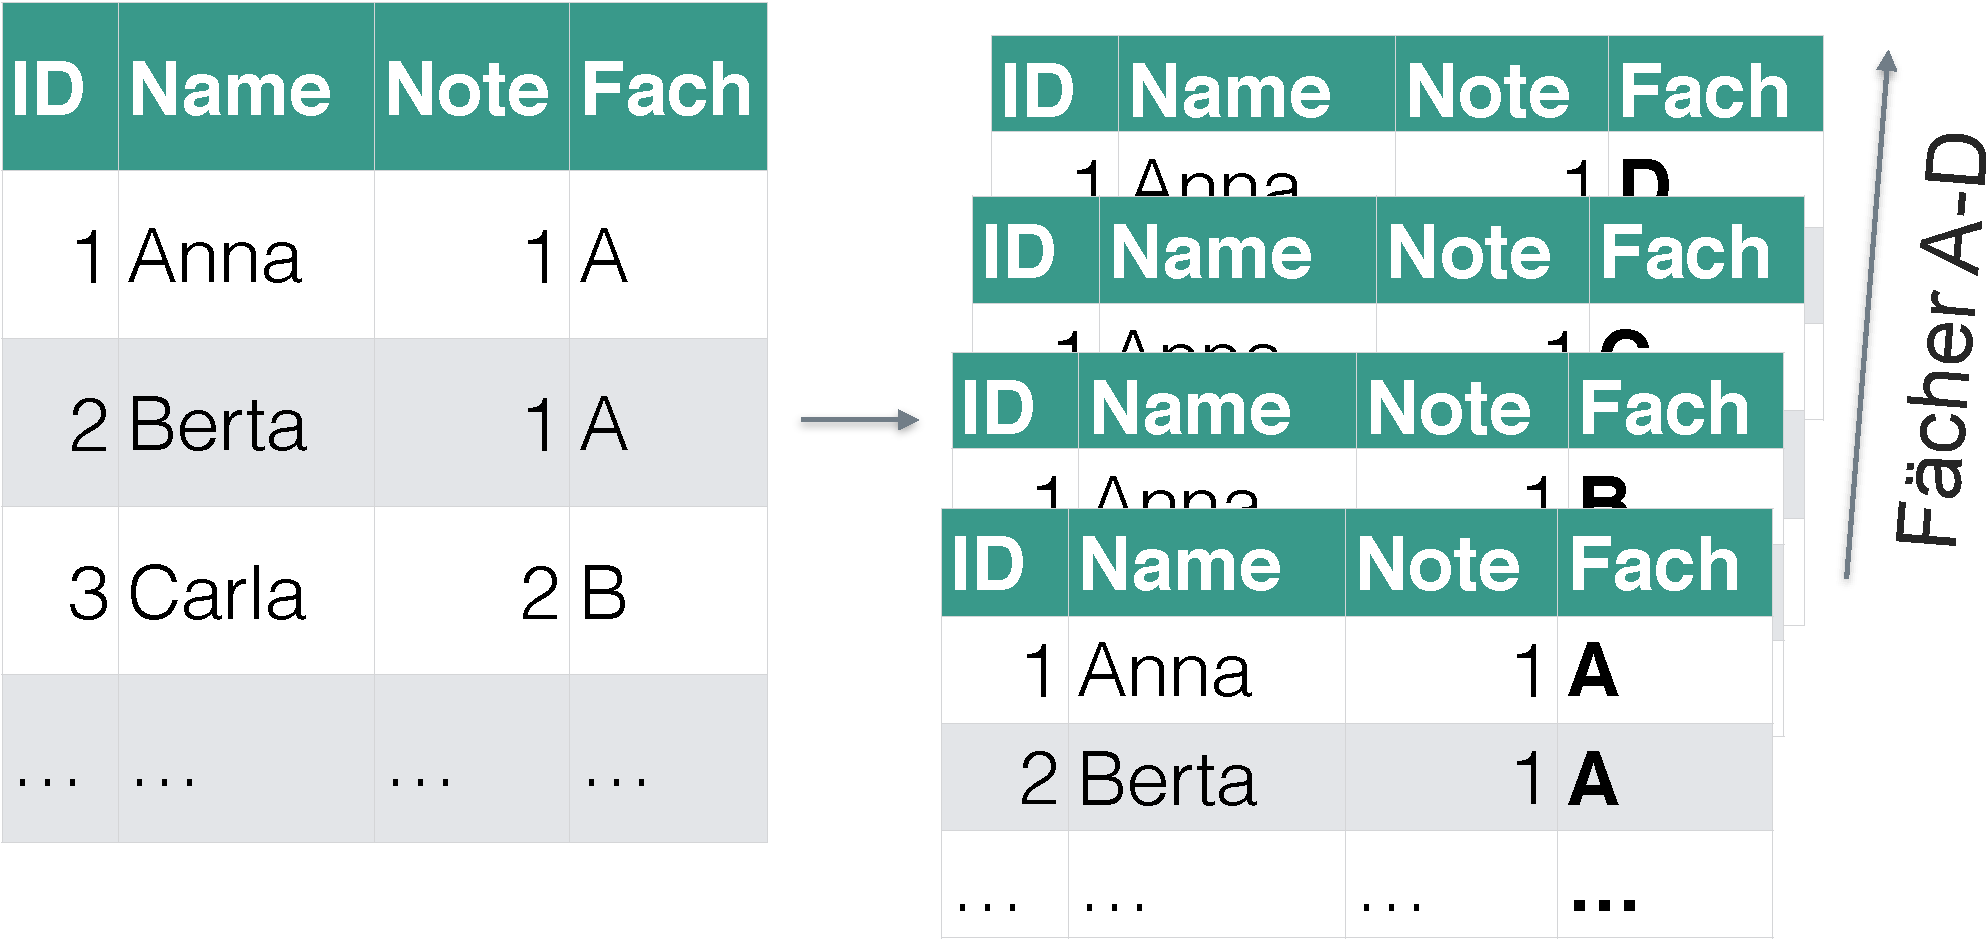
\includegraphics[width=0.7\linewidth]{images/Datenjudo/group_by} 

}

\caption{Datensätze nach Subgruppen aufteilen}\label{fig:fig-groupby}
\end{figure}

In Abbildung \ref{fig:fig-groupby} wurde der Datensatz anhand der Spalte
(d.h. Variable) \texttt{Fach} in mehrere Gruppen geteilt (Fach A, Fach
B\ldots{}). Wir könnten uns als nächstes z.B. Mittelwerte pro Fach -
d.h. pro Gruppe (pro Ausprägung von \texttt{Fach}) - ausgeben lassen; in
diesem Fall vier Gruppen (Fach A bis D).

\begin{Shaded}
\begin{Highlighting}[]
\NormalTok{test_gruppiert <-}\StringTok{ }\KeywordTok{group_by}\NormalTok{(stats_test, interest)}
\NormalTok{test_gruppiert}
\CommentTok{#> Source: local data frame [306 x 6]}
\CommentTok{#> Groups: interest [7]}
\CommentTok{#> }
\CommentTok{#> # A tibble: 306 x 6}
\CommentTok{#>    row_number           date_time study_time self_eval interest score}
\CommentTok{#>         <int>               <chr>      <int>     <int>    <int> <int>}
\CommentTok{#>  1          1 05.01.2017 13:57:01          5         8        5    29}
\CommentTok{#>  2          2 05.01.2017 21:07:56          3         7        3    29}
\CommentTok{#>  3          3 05.01.2017 23:33:47          5        10        6    40}
\CommentTok{#>  4          4 06.01.2017 09:58:05          2         3        2    18}
\CommentTok{#>  5          5 06.01.2017 14:13:08          4         8        6    34}
\CommentTok{#>  6          6 06.01.2017 14:21:18         NA        NA       NA    39}
\CommentTok{#>  7          7 06.01.2017 14:25:49         NA        NA       NA    40}
\CommentTok{#>  8          8 06.01.2017 17:24:53          2         5        3    24}
\CommentTok{#>  9          9 07.01.2017 10:11:17          2         3        5    25}
\CommentTok{#> 10         10 07.01.2017 18:10:05          4         5        5    33}
\CommentTok{#> # ... with 296 more rows}
\end{Highlighting}
\end{Shaded}

Schaut man sich nun den Datensatz an, sieht man erstmal wenig Effekt der
Gruppierung. R teilt uns lediglich mit
\texttt{Groups:\ interest\ {[}7{]}}, dass es 7 Gruppen gibt, aber es
gibt keine extra Spalte oder sonstige Anzeichen der Gruppierung. Aber
keine Sorge, wenn wir gleich einen Mittelwert ausrechnen, bekommen wir
den Mittelwert pro Gruppe!

Ein paar Hinweise: \texttt{Source:\ local\ data\ frame\ {[}306\ x\ 6{]}}
will sagen, dass die Ausgabe sich auf einen \texttt{tibble}
bezieht\footnote{\url{http://stackoverflow.com/questions/29084380/what-is-the-meaning-of-the-local-data-frame-message-from-dplyrprint-tbl-df}},
also eine bestimmte Art von Dataframe.
\texttt{Groups:\ interest\ {[}7{]}} zeigt, dass der Tibble in 7 Gruppen
- entsprechend der Werte von \texttt{interest} aufgeteilt ist.

\texttt{group\_by} an sich ist nicht wirklich nützlich. Nützlich wird es
erst, wenn man weitere Funktionen auf den gruppierten Datensatz anwendet
- z.B. Mittelwerte ausrechnet (z.B mit \texttt{summarise}, s. unten).
Die nachfolgenden Funktionen (wenn sie aus \texttt{dplyr} kommen),
berücksichtigen nämlich die Gruppierung. So kann man einfach Mittelwerte
pro Gruppe ausrechnen. \texttt{dplyr} kombiniert dann die
Zusammenfassungen (z.B. Mittelwerte) der einzelnen Gruppen in einen
Dataframe und gibt diesen dann aus.

Die Idee des ``Gruppieren - Zusammenfassen - Kombinieren'' ist flexibel;
man kann sie häufig brauchen. Es lohnt sich, diese Idee zu lernen (vgl.
Abb. \ref{fig:sac}).

\begin{figure}

{\centering 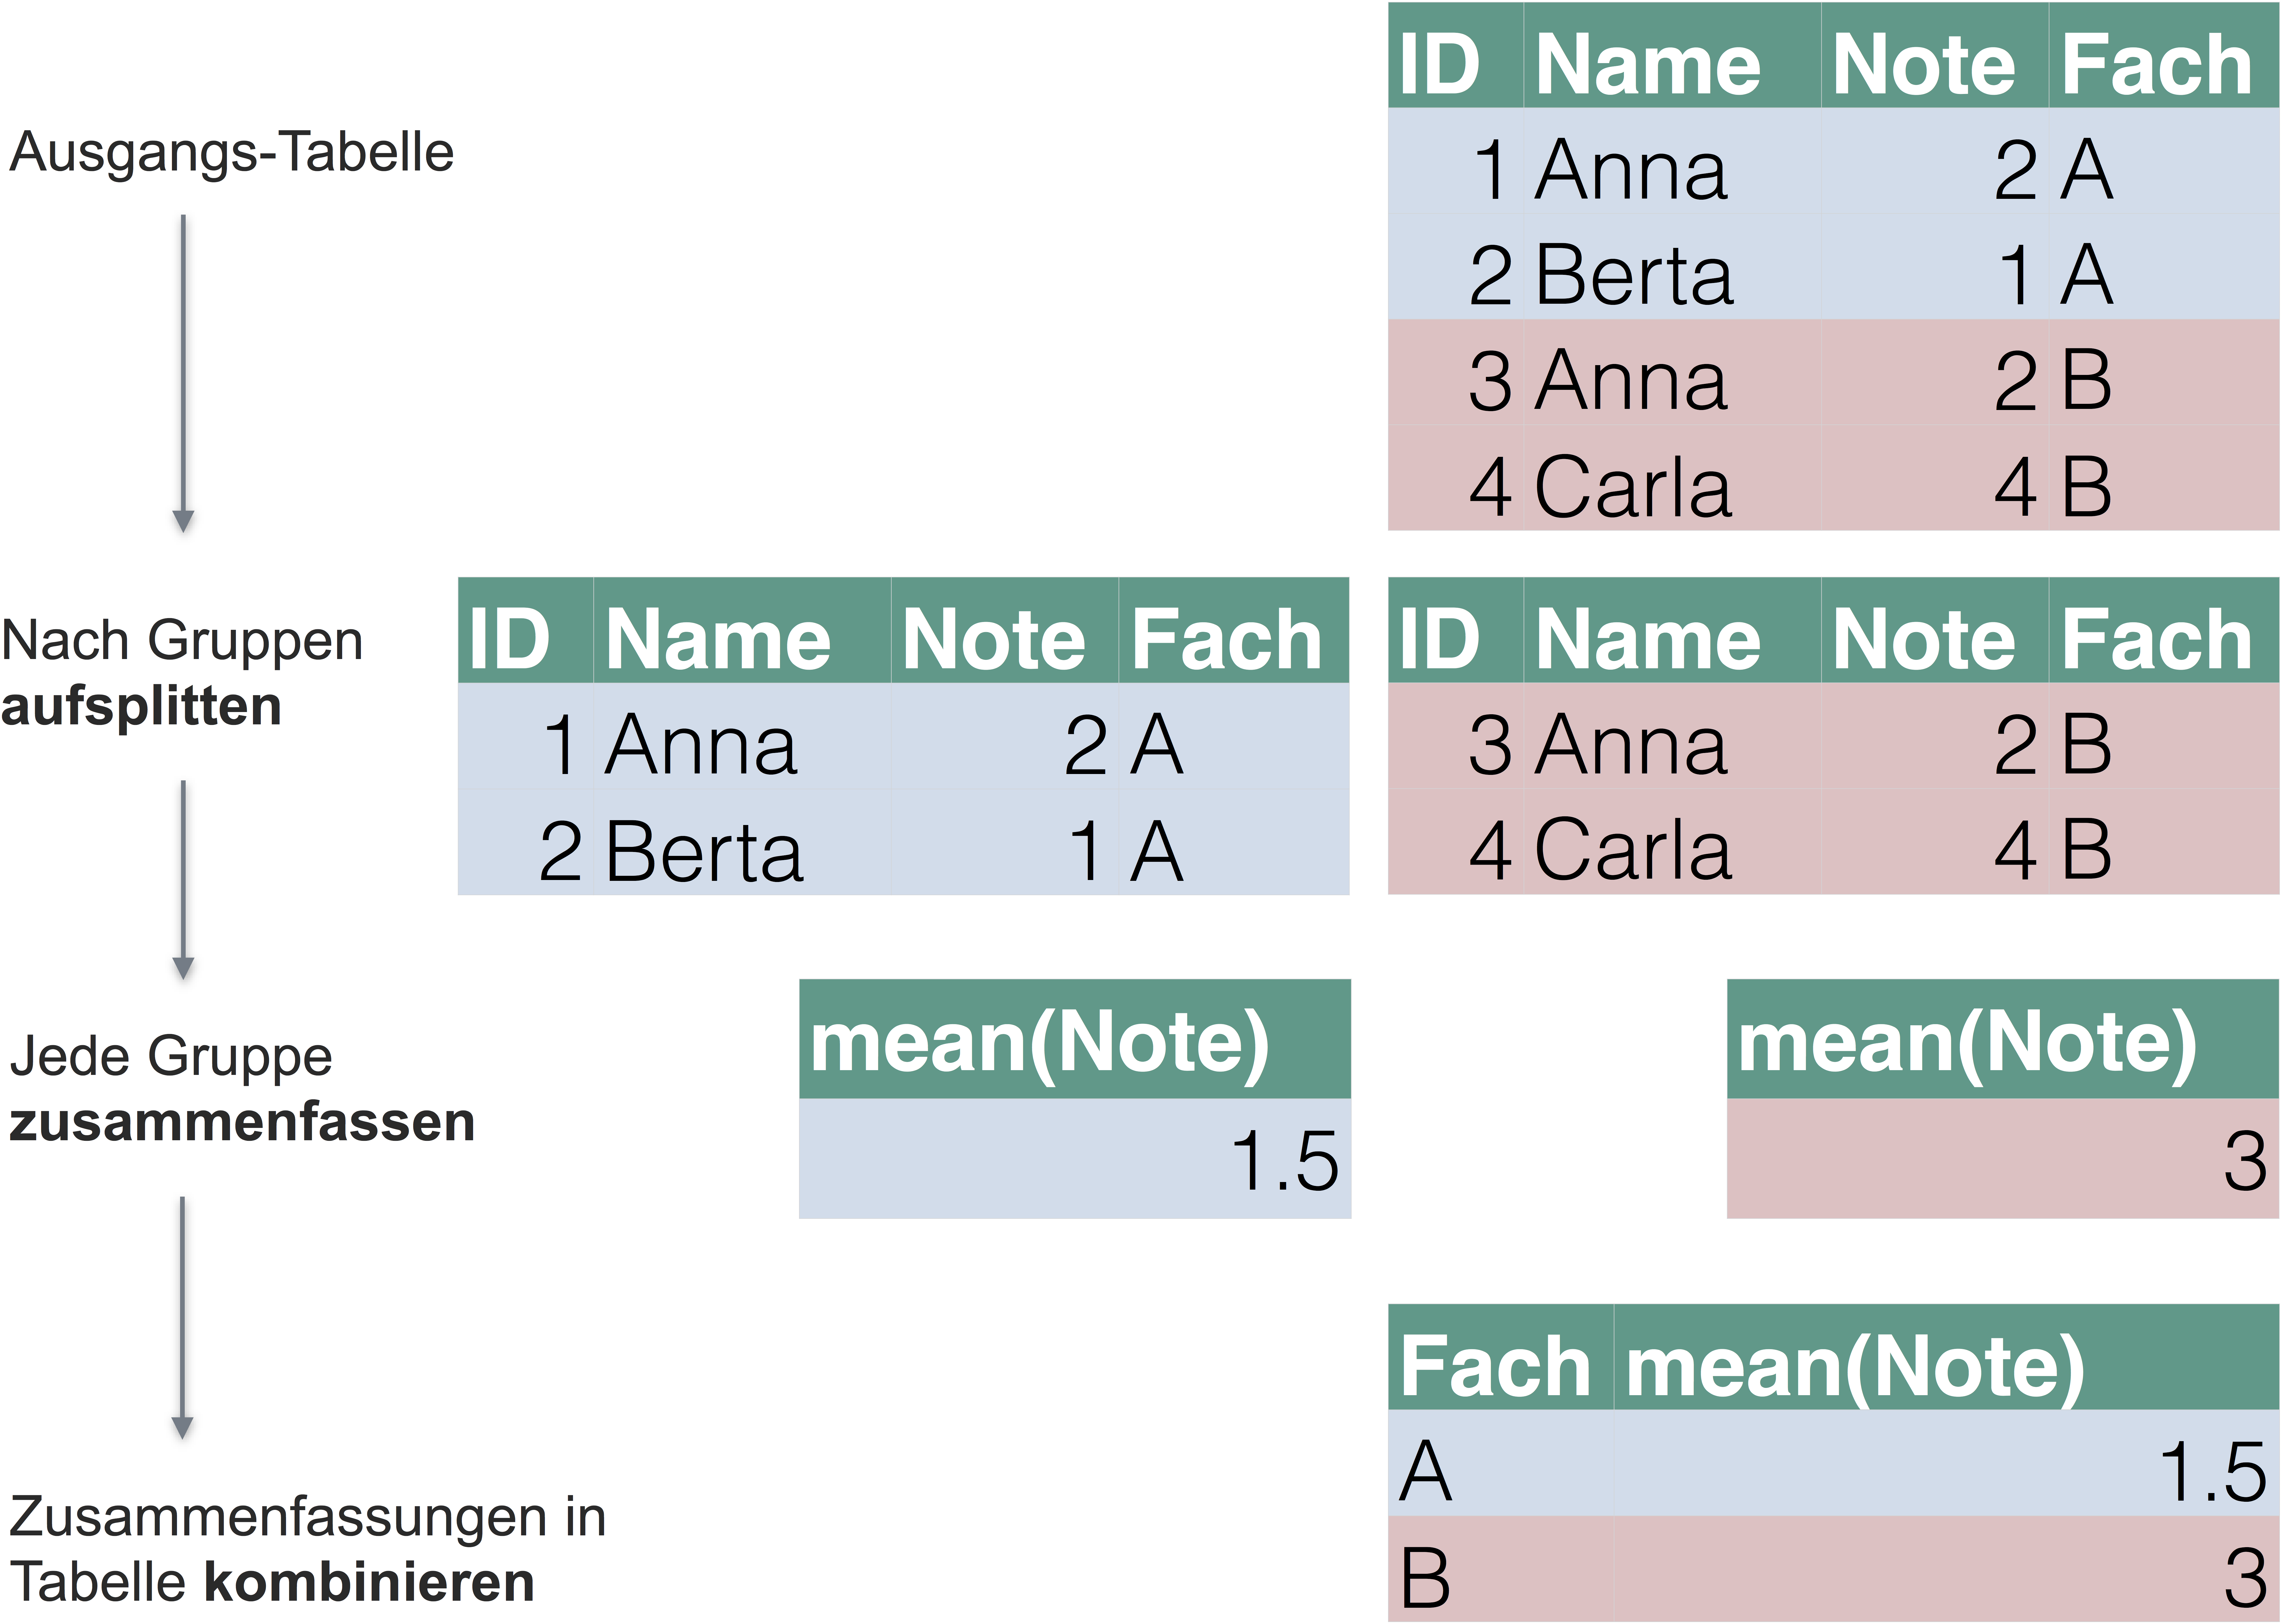
\includegraphics[width=0.7\linewidth]{images/Datenjudo/sac_crop} 

}

\caption{Schematische Darstellung des 'Gruppieren - Zusammenfassen - Kombinieren'}\label{fig:sac}
\end{figure}

\subsubsection[Aufgaben]{\texorpdfstring{Aufgaben\footnote{R, F, R, R}}{Aufgaben}}\label{aufgaben-6}

\BeginKnitrBlock{rmdexercises}
Richtig oder Falsch!?

\begin{enumerate}
\def\labelenumi{\arabic{enumi}.}
\tightlist
\item
  Mit \texttt{group\_by} gruppiert man einen Datensatz.
\item
  \texttt{group\_by} lässt nur ein Gruppierungskriterium zu.
\item
  Die Gruppierung durch \texttt{group\_by} wird nur von Funktionen aus
  \texttt{dplyr} erkannt.
\item
  \texttt{group\_by} ist sinnvoll mit \texttt{summarise} zu kombinieren.
\end{enumerate}
\EndKnitrBlock{rmdexercises}

Merke:

\begin{quote}
Mit group\_by teilt man einen Datensatz in Gruppen ein, entsprechend der
Werte einer mehrerer Spalten.
\end{quote}

\subsection{\texorpdfstring{Eine Spalte zusammenfassen mit
\texttt{summarise}}{Eine Spalte zusammenfassen mit summarise}}\label{eine-spalte-zusammenfassen-mit-summarise}

Vielleicht die wichtigste oder häufigte Tätigkeit in der Analyse von
Daten ist es, eine Spalte zu \emph{einem} Wert zusammenzufassen;
\texttt{summarise}\index{dplyr::summarise} leistet dies. Anders gesagt:
Einen Mittelwert berechnen, den größten (kleinsten) Wert heraussuchen,
die Korrelation berechnen oder eine beliebige andere Statistik ausgeben
lassen. Die Gemeinsamkeit dieser Operaitonen ist, dass sie eine Spalte
zu einem Wert zusammenfassen, ``aus Spalte mach Zahl'', sozusagen. Daher
ist der Name des Befehls \texttt{summarise} ganz passend. Genauer gesagt
fasst dieser Befehl eine Spalte zu einer Zahl zusammen \emph{anhand}
einer Funktion wie \texttt{mean} oder \texttt{max} (vgl. Abb.
\ref{fig:fig-summarise}. Hierbei ist jede Funktion erlaubt, die eine
Spalte als Input verlangt und eine Zahl zurückgibt; andere Funktionen
sind bei \texttt{summarise} nicht erlaubt.

\begin{figure}

{\centering 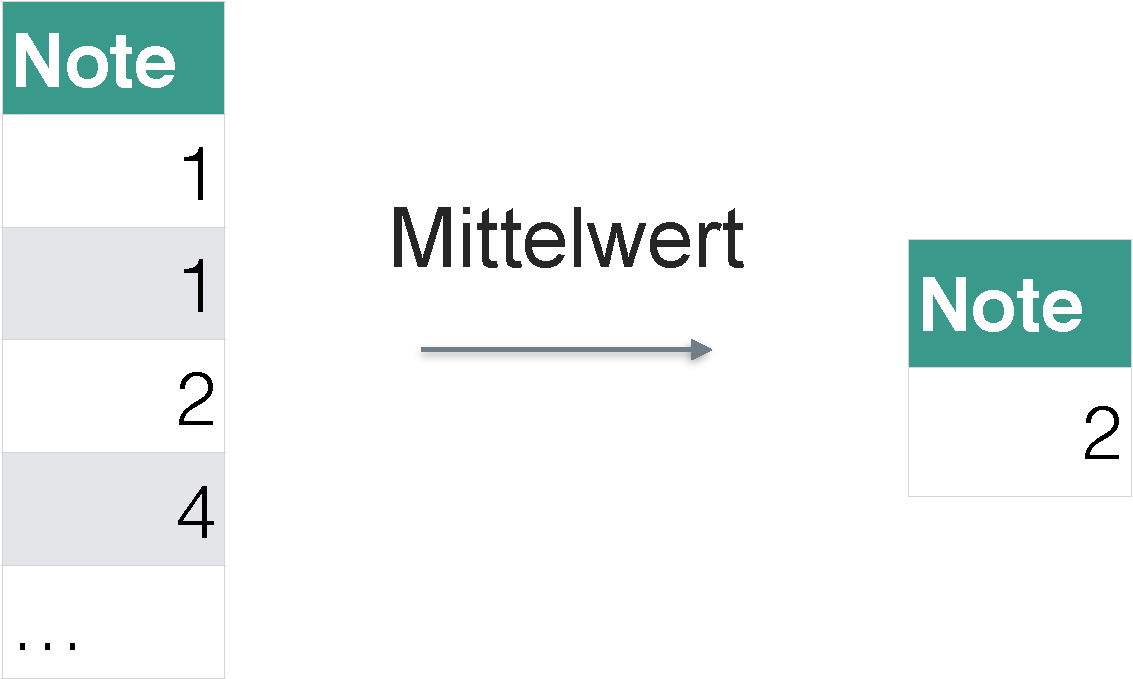
\includegraphics[width=0.7\linewidth]{images/Datenjudo/summarise} 

}

\caption{Spalten zu einer Zahl zusammenfassen}\label{fig:fig-summarise}
\end{figure}

\begin{Shaded}
\begin{Highlighting}[]
\KeywordTok{summarise}\NormalTok{(stats_test, }\KeywordTok{mean}\NormalTok{(score))}
\CommentTok{#> # A tibble: 1 x 1}
\CommentTok{#>   `mean(score)`}
\CommentTok{#>           <dbl>}
\CommentTok{#> 1          31.1}
\end{Highlighting}
\end{Shaded}

Man könnte diesen Befehl so ins Deutsche übersetzen:
\texttt{Fasse\ aus\ Tabelle\ stats\_test\ die\ Spalte\ score\ anhand\ des\ Mittelwerts\ zusammen}.
Nicht vergessen, wenn die Spalte \texttt{score} fehlende Werte hat, wird
der Befehl \texttt{mean} standardmäßig dies mit \texttt{NA} quittieren.
Ergänzt man den Parameter \texttt{nr.rm\ =\ TRUE}, so ignoriert R
fehlende Werte und der Befehl \texttt{mean} liefert ein Ergebnis zurück.

Jetzt können wir auch die Gruppierung nutzen:

\begin{Shaded}
\begin{Highlighting}[]
\NormalTok{test_gruppiert <-}\StringTok{ }\KeywordTok{group_by}\NormalTok{(stats_test, interest)}
\KeywordTok{summarise}\NormalTok{(test_gruppiert, }\KeywordTok{mean}\NormalTok{(score, }\DataTypeTok{na.rm =} \OtherTok{TRUE}\NormalTok{))}
\CommentTok{#> # A tibble: 7 x 2}
\CommentTok{#>   interest `mean(score, na.rm = TRUE)`}
\CommentTok{#>      <int>                       <dbl>}
\CommentTok{#> 1        1                        28.3}
\CommentTok{#> 2        2                        29.7}
\CommentTok{#> 3        3                        30.8}
\CommentTok{#> 4        4                        29.9}
\CommentTok{#> 5        5                        32.5}
\CommentTok{#> 6        6                        34.0}
\CommentTok{#> 7       NA                        33.1}
\end{Highlighting}
\end{Shaded}

Der Befehl \texttt{summarise} erkennt also, wenn eine (mit
\texttt{group\_by}) gruppierte Tabelle vorliegt. Jegliche
Zusammenfassung, die wir anfordern, wird anhand der
Gruppierungsinformation aufgeteilt werden. In dem Beispiel bekommen wir
einen Mittelwert für jeden Wert von \texttt{interest}.
Interessanterweise sehen wir, dass der Mittelwert tendenziell größer
wird, je größer \texttt{interest} wird.

Alle diese \texttt{dplyr}-Befehle geben einen Dataframe zurück, was
praktisch ist für weitere Verarbeitung. In diesem Fall heißen die
Spalten \texttt{interst} und \texttt{mean(score)}. Zweiter Name ist
nicht so schön, daher ändern wir den wie folgt:

Jetzt können wir auch die Gruppierung nutzen:

\begin{Shaded}
\begin{Highlighting}[]
\NormalTok{test_gruppiert <-}\StringTok{ }\KeywordTok{group_by}\NormalTok{(stats_test, interest)}
\KeywordTok{summarise}\NormalTok{(test_gruppiert, }\DataTypeTok{mw_pro_gruppe =} \KeywordTok{mean}\NormalTok{(score, }\DataTypeTok{na.rm =} \OtherTok{TRUE}\NormalTok{))}
\CommentTok{#> # A tibble: 7 x 2}
\CommentTok{#>   interest mw_pro_gruppe}
\CommentTok{#>      <int>         <dbl>}
\CommentTok{#> 1        1          28.3}
\CommentTok{#> 2        2          29.7}
\CommentTok{#> 3        3          30.8}
\CommentTok{#> 4        4          29.9}
\CommentTok{#> 5        5          32.5}
\CommentTok{#> 6        6          34.0}
\CommentTok{#> 7       NA          33.1}
\end{Highlighting}
\end{Shaded}

Nun heißt die zweite Spalte \texttt{mw\_pro\_Gruppe}.
\texttt{na.rm\ =\ TRUE} veranlasst, bei fehlenden Werten trotzdem einen
Mittelwert zurückzuliefern (die Zeilen mit fehlenden Werten werden in
dem Fall ignoriert).

Grundsätzlich ist die Philosophie der \texttt{dplyr}-Befehle: ``Mach nur
eine Sache, aber die dafür gut''. Entsprechend kann \texttt{summarise}
nur \emph{Spalten} zusammenfassen, aber keine \emph{Zeilen}.

Merke:

\begin{quote}
Mit summarise kann man eine Spalte eines Dataframes zu einem Wert
zusammenfassen.
\end{quote}

\subsubsection{\texorpdfstring{Deskriptive Statistik mit
\texttt{summarise}}{Deskriptive Statistik mit summarise}}\label{deskriptive-statistik-mit-summarise}

\begin{quote}
Die deskriptive Statistik hat zwei Haupt-Bereiche: Lagemaße und
Streuungsmaße.
\end{quote}

\emph{Lagemaße} geben den ``typischen'', ``mittleren'' oder
``repräsentativen'' Vertreter der Verteilung an. Bei den
Lagemaßen\index{Lagemaße} denkt man sofort an das \emph{arithmetische
Mittel} (synonym: Mittelwert; häufig als \(\bar{X}\) abgekürzt;
\texttt{mean}). Ein Nachteil von Mittelwerten ist, dass sie nicht robust
gegenüber Extremwerte sind: Schon ein vergleichsweise großer Einzelwert
kann den Mittelwert deutlich verändern und damit die Repräsentativität
des Mittelwerts für die Gesamtmenge der Daten in Frage stellen. Eine
robuste Variante ist der \emph{Median} (Md; \texttt{median}). Ist die
Anzahl der (unterschiedlichen) Ausprägungen nicht zu groß im Verhältnis
zur Fallzahl, so ist der \emph{Modus} eine sinnvolle Statistik; er gibt
die häufigste Ausprägung an\footnote{Der \emph{Modus} ist im Standard-R
  nicht mit einem eigenen Befehl vertreten. Man kann ihn aber leicht von
  Hand bestimmen; s.u. Es gibt auch einige Pakete, die diese Funktion
  anbieten: z.B.
  \url{https://cran.r-project.org/web/packages/modes/index.html}}.

\emph{Streuungsmaße}\index{Streuungsmaße} geben die Unterschiedlichkeit
in den Daten wieder; mit anderen Worten: sind die Daten sich ähnlich
oder unterscheiden sich die Werte deutlich? Zentrale Statistiken sind
der \emph{mittlere Absolutabstand} (MAA; MAD),\footnote{Der \emph{MAD}
  ist im Standard-R nicht mit einem eigenen Befehl vertreten. Es gibt
  einige Pakete, die diese Funktion anbieten: z.B.
  \url{https://artax.karlin.mff.cuni.cz/r-help/library/lsr/html/aad.html}}
die \emph{Standardabweichung} (sd; \texttt{sd}), die \emph{Varianz}
(Var; \texttt{var}) und der \emph{Interquartilsabstand} (IQR;
\texttt{IQR}). Da nur der IQR \emph{nicht} auf dem Mittelwert basiert,
ist er am robustesten. Beliebige Quantile bekommt man mit dem R-Befehl
\texttt{quantile}.

Der Befehl \texttt{summarise} eignet sich, um deskriptive Statistiken
auszurechnen.

\begin{Shaded}
\begin{Highlighting}[]
\KeywordTok{summarise}\NormalTok{(stats_test, }\KeywordTok{mean}\NormalTok{(score))}
\CommentTok{#> # A tibble: 1 x 1}
\CommentTok{#>   `mean(score)`}
\CommentTok{#>           <dbl>}
\CommentTok{#> 1          31.1}
\KeywordTok{summarise}\NormalTok{(stats_test, }\KeywordTok{sd}\NormalTok{(score))}
\CommentTok{#> # A tibble: 1 x 1}
\CommentTok{#>   `sd(score)`}
\CommentTok{#>         <dbl>}
\CommentTok{#> 1        5.74}
\end{Highlighting}
\end{Shaded}

Natürlich könnte man auch einfacher schreiben:

\begin{Shaded}
\begin{Highlighting}[]
\KeywordTok{mean}\NormalTok{(stats_test$score)}
\CommentTok{#> [1] 31.1}
\KeywordTok{median}\NormalTok{(stats_test$score)}
\CommentTok{#> [1] 31}
\end{Highlighting}
\end{Shaded}

\texttt{summarise} liefert aber im Unterschied zu \texttt{mean} etc.
immer einen Dataframe zurück. Da der Dataframe die typische
Datenstruktur ist, ist es häufig praktisch, wenn man einen Dataframe
zurückbekommt, mit dem man weiterarbeiten kann. Außerdem lassen
\texttt{mean} etc. keine Gruppierungsoperationen zu; über
\texttt{group\_by} kann man dies aber bei \texttt{dplyr} erreichen.

\subsubsection[Aufgaben]{\texorpdfstring{Aufgaben\footnote{R, R, R, R, R}}{Aufgaben}}\label{aufgaben-7}

\BeginKnitrBlock{rmdexercises}
Richtig oder Falsch!?

\begin{enumerate}
\def\labelenumi{\arabic{enumi}.}
\tightlist
\item
  Möchte man aus der Tabelle \texttt{stats\_test} den Mittelwert für die
  Spalte \texttt{score} berechnen, so ist folgende Syntax korrekt:
  \texttt{summarise(stats\_test,\ mean(score))}.
\item
  \texttt{summarise} liefert eine Tabelle, genauer: einen Tibble,
  zurück.
\item
  Die Tabelle, die diese Funktion zurückliefert:
  \texttt{summarise(stats\_test,\ mean(score))}, hat eine Spalte mit dem
  Namen \texttt{mean(score)}.
\item
  \texttt{summarise} lässt zu, dass die zu berechnende Spalte einen
  Namen vom Nutzer zugewiesen bekommt.
\item
  \texttt{summarise} darf nur verwendet werden, wenn eine Spalte zu
  einem Wert zusammengefasst werden soll.
\end{enumerate}
\EndKnitrBlock{rmdexercises}

\begin{enumerate}
\def\labelenumi{\arabic{enumi}.}
\tightlist
\item
  (Fortgeschritten) Bauen Sie einen eigenen Weg, um den mittleren
  Absolutabstand auszurechnen! Gehen Sie der Einfachheit halber (zuerst)
  von einem Vektor mit den Werten (1,2,3) aus!
\end{enumerate}

Lösung:

\begin{Shaded}
\begin{Highlighting}[]
\NormalTok{x <-}\StringTok{ }\KeywordTok{c}\NormalTok{(}\DecValTok{1}\NormalTok{, }\DecValTok{2}\NormalTok{, }\DecValTok{3}\NormalTok{)}
\NormalTok{x_mw <-}\StringTok{ }\KeywordTok{mean}\NormalTok{(x)}
\NormalTok{x_delta <-}\StringTok{ }\NormalTok{x -}\StringTok{ }\NormalTok{x_mw}
\NormalTok{x_delta <-}\StringTok{ }\KeywordTok{abs}\NormalTok{(x_delta)}
\NormalTok{mad <-}\StringTok{ }\KeywordTok{mean}\NormalTok{(x_delta)}
\NormalTok{mad}
\CommentTok{#> [1] 0.667}
\end{Highlighting}
\end{Shaded}

\subsection{\texorpdfstring{Zeilen zählen mit \texttt{n} und
\texttt{count}}{Zeilen zählen mit n und count}}\label{zeilen-zahlen-mit-n-und-count}

Ebenfalls nützlich ist es, Zeilen zu zählen. Im Gegensatz zum
Standardbefehl\footnote{Standardbefehl meint, dass die Funktion zum
  Standardrepertoire von R gehört, also nicht über ein Paket extra
  geladen werden muss} \texttt{nrow} versteht der \texttt{dyplr}-Befehl
\texttt{n}\index{dplyr::n} auch Gruppierungen. \texttt{n} darf nur
innerhalb von \texttt{summarise} oder ähnlichen \texttt{dplyr}-Befehlen
verwendet werden.

\begin{Shaded}
\begin{Highlighting}[]
\KeywordTok{summarise}\NormalTok{(stats_test, }\KeywordTok{n}\NormalTok{())}
\CommentTok{#> # A tibble: 1 x 1}
\CommentTok{#>   `n()`}
\CommentTok{#>   <int>}
\CommentTok{#> 1   306}
\KeywordTok{summarise}\NormalTok{(test_gruppiert, }\KeywordTok{n}\NormalTok{())}
\CommentTok{#> # A tibble: 7 x 2}
\CommentTok{#>   interest `n()`}
\CommentTok{#>      <int> <int>}
\CommentTok{#> 1        1    30}
\CommentTok{#> 2        2    47}
\CommentTok{#> 3        3    66}
\CommentTok{#> 4        4    41}
\CommentTok{#> 5        5    45}
\CommentTok{#> 6        6     9}
\CommentTok{#> 7       NA    68}
\KeywordTok{nrow}\NormalTok{(stats_test)}
\CommentTok{#> [1] 306}
\end{Highlighting}
\end{Shaded}

Außerhalb von gruppierten Datensätzen ist \texttt{nrow} meist
praktischer.

Praktischer ist der Befehl \texttt{count}\index{dplyr::count}, der
nichts anderes ist als die Hintereinanderschaltung von
\texttt{group\_by} und \texttt{n}. Mit \texttt{count} zählen wir die
Häufigkeiten nach Gruppen; Gruppen sind hier zumeist die Werte einer
auszuzählenden Variablen (oder mehrerer auszuzählender Variablen). Das
macht \texttt{count} zu einem wichtigen Helfer bei der Analyse von
Häufigkeitsdaten.

\begin{Shaded}
\begin{Highlighting}[]
\NormalTok{dplyr::}\KeywordTok{count}\NormalTok{(stats_test, interest)}
\CommentTok{#> # A tibble: 7 x 2}
\CommentTok{#>   interest     n}
\CommentTok{#>      <int> <int>}
\CommentTok{#> 1        1    30}
\CommentTok{#> 2        2    47}
\CommentTok{#> 3        3    66}
\CommentTok{#> 4        4    41}
\CommentTok{#> 5        5    45}
\CommentTok{#> 6        6     9}
\CommentTok{#> 7       NA    68}
\NormalTok{dplyr::}\KeywordTok{count}\NormalTok{(stats_test, study_time)}
\CommentTok{#> # A tibble: 6 x 2}
\CommentTok{#>   study_time     n}
\CommentTok{#>        <int> <int>}
\CommentTok{#> 1          1    31}
\CommentTok{#> 2          2    49}
\CommentTok{#> 3          3    85}
\CommentTok{#> 4          4    56}
\CommentTok{#> 5          5    17}
\CommentTok{#> 6         NA    68}
\NormalTok{dplyr::}\KeywordTok{count}\NormalTok{(stats_test, interest, study_time)}
\CommentTok{#> Source: local data frame [29 x 3]}
\CommentTok{#> Groups: interest [?]}
\CommentTok{#> }
\CommentTok{#> # A tibble: 29 x 3}
\CommentTok{#>    interest study_time     n}
\CommentTok{#>       <int>      <int> <int>}
\CommentTok{#>  1        1          1    12}
\CommentTok{#>  2        1          2     7}
\CommentTok{#>  3        1          3     8}
\CommentTok{#>  4        1          4     2}
\CommentTok{#>  5        1          5     1}
\CommentTok{#>  6        2          1     9}
\CommentTok{#>  7        2          2    15}
\CommentTok{#>  8        2          3    16}
\CommentTok{#>  9        2          4     6}
\CommentTok{#> 10        2          5     1}
\CommentTok{#> # ... with 19 more rows}
\end{Highlighting}
\end{Shaded}

Allgemeiner formuliert lautet die Syntax:
\texttt{count(df,\ Spalte1,\ ...)}, wobei \texttt{df} der Dataframe ist
und \texttt{Spalte1} die erste (es können mehrere sein) auszuzählende
Spalte. Gibt man z.B. zwei Spalten an, so wird pro Wert der 1. Spalte
die Häufigkeiten der 2. Spalte ausgegeben.

Merke:

\begin{quote}
n und count zählen die Anzahl der Zeilen, d.h. die Anzahl der Fälle.
\end{quote}

\subsubsection{Vertiefung zum Zählen von Zeilen: Relative
Häufigkeiten}\label{vertiefung-zum-zahlen-von-zeilen-relative-haufigkeiten}

Manchmal ist es praktisch, nicht zur die (absolute) Häufigkeiten von
Zeilen zu zählen, sondern ihren Anteil nach (relative Häufigkeit).
Klassisches Beispiel: Wieviel Prozent der Fälle sind Frauen, wie viele
sind Männer?

In \texttt{dplyr} kann man das so umsetzen:

\begin{Shaded}
\begin{Highlighting}[]
\NormalTok{stats_test %>%}\StringTok{ }
\StringTok{  }\KeywordTok{count}\NormalTok{(interest) %>%}\StringTok{ }
\StringTok{  }\KeywordTok{mutate}\NormalTok{(}\DataTypeTok{prop_interest =} \NormalTok{n /}\StringTok{ }\KeywordTok{sum}\NormalTok{(n))}
\CommentTok{#> # A tibble: 7 x 3}
\CommentTok{#>   interest     n prop_interest}
\CommentTok{#>      <int> <int>         <dbl>}
\CommentTok{#> 1        1    30        0.0980}
\CommentTok{#> 2        2    47        0.1536}
\CommentTok{#> 3        3    66        0.2157}
\CommentTok{#> 4        4    41        0.1340}
\CommentTok{#> 5        5    45        0.1471}
\CommentTok{#> 6        6     9        0.0294}
\CommentTok{#> 7       NA    68        0.2222}
\end{Highlighting}
\end{Shaded}

\texttt{prop} steht hier für ``Proportion'', also Anteil.
\texttt{sum(n)} liefert die Summe der Fälle zurück, also 306 in diesem
Fall.

Etwas komplexer ist es, wenn man zwei Gruppierungsvariablen hat und dann
Anteile auszählen möchte:

\begin{Shaded}
\begin{Highlighting}[]

\NormalTok{stats_test$bestanden <-}\StringTok{ }\NormalTok{stats_test$score >}\StringTok{ }\DecValTok{25}

\NormalTok{stats_test %>%}\StringTok{ }
\StringTok{  }\KeywordTok{group_by}\NormalTok{(interest, bestanden) %>%}\StringTok{ }
\StringTok{  }\KeywordTok{summarise}\NormalTok{(}\DataTypeTok{n =} \KeywordTok{n}\NormalTok{()) %>%}\StringTok{ }
\StringTok{  }\KeywordTok{mutate}\NormalTok{(}\DataTypeTok{prop_interest =} \NormalTok{n /}\StringTok{ }\KeywordTok{sum}\NormalTok{(n)) }
\CommentTok{#> Source: local data frame [14 x 4]}
\CommentTok{#> Groups: interest [7]}
\CommentTok{#> }
\CommentTok{#> # A tibble: 14 x 4}
\CommentTok{#>    interest bestanden     n prop_interest}
\CommentTok{#>       <int>     <lgl> <int>         <dbl>}
\CommentTok{#>  1        1     FALSE    10         0.333}
\CommentTok{#>  2        1      TRUE    20         0.667}
\CommentTok{#>  3        2     FALSE     9         0.191}
\CommentTok{#>  4        2      TRUE    38         0.809}
\CommentTok{#>  5        3     FALSE    14         0.212}
\CommentTok{#>  6        3      TRUE    52         0.788}
\CommentTok{#>  7        4     FALSE     9         0.220}
\CommentTok{#>  8        4      TRUE    32         0.780}
\CommentTok{#>  9        5     FALSE     6         0.133}
\CommentTok{#> 10        5      TRUE    39         0.867}
\CommentTok{#> 11        6     FALSE     1         0.111}
\CommentTok{#> 12        6      TRUE     8         0.889}
\CommentTok{#> 13       NA     FALSE     7         0.103}
\CommentTok{#> 14       NA      TRUE    61         0.897}

\NormalTok{stats_test %>%}\StringTok{ }
\StringTok{  }\KeywordTok{count}\NormalTok{(interest, bestanden) %>%}\StringTok{ }
\StringTok{  }\KeywordTok{mutate}\NormalTok{(}\DataTypeTok{prop_interest =} \NormalTok{n /}\StringTok{ }\KeywordTok{sum}\NormalTok{(n)) }
\CommentTok{#> Source: local data frame [14 x 4]}
\CommentTok{#> Groups: interest [7]}
\CommentTok{#> }
\CommentTok{#> # A tibble: 14 x 4}
\CommentTok{#>    interest bestanden     n prop_interest}
\CommentTok{#>       <int>     <lgl> <int>         <dbl>}
\CommentTok{#>  1        1     FALSE    10         0.333}
\CommentTok{#>  2        1      TRUE    20         0.667}
\CommentTok{#>  3        2     FALSE     9         0.191}
\CommentTok{#>  4        2      TRUE    38         0.809}
\CommentTok{#>  5        3     FALSE    14         0.212}
\CommentTok{#>  6        3      TRUE    52         0.788}
\CommentTok{#>  7        4     FALSE     9         0.220}
\CommentTok{#>  8        4      TRUE    32         0.780}
\CommentTok{#>  9        5     FALSE     6         0.133}
\CommentTok{#> 10        5      TRUE    39         0.867}
\CommentTok{#> 11        6     FALSE     1         0.111}
\CommentTok{#> 12        6      TRUE     8         0.889}
\CommentTok{#> 13       NA     FALSE     7         0.103}
\CommentTok{#> 14       NA      TRUE    61         0.897}
\end{Highlighting}
\end{Shaded}

\subsubsection[Aufgaben]{\texorpdfstring{Aufgaben\footnote{R, R, F, F}}{Aufgaben}}\label{aufgaben-8}

\BeginKnitrBlock{rmdexercises}
Richtig oder Falsch!?

\begin{enumerate}
\def\labelenumi{\arabic{enumi}.}
\tightlist
\item
  Mit \texttt{count} kann man Zeilen zählen.
\item
  \texttt{count} ist ähnlich (oder identisch) zu einer Kombination von
  \texttt{group\_by} und \texttt{n()}.
\item
  Mit \texttt{count} kann man nur nur eine Gruppe beim Zählen
  berücksichtigen.
\item
  \texttt{count} darf nicht bei nominalskalierten Variablen verwendet
  werden.
\end{enumerate}
\EndKnitrBlock{rmdexercises}

\begin{enumerate}
\def\labelenumi{\arabic{enumi}.}
\tightlist
\item
  Bauen Sie sich einen Weg, um den Modus mithilfe von \texttt{count} und
  \texttt{arrange} zu bekommen!
\end{enumerate}

\begin{Shaded}
\begin{Highlighting}[]
\NormalTok{stats_count <-}\StringTok{ }\KeywordTok{count}\NormalTok{(stats_test, score)}
\NormalTok{stats_count_sortiert <-}\StringTok{ }\KeywordTok{arrange}\NormalTok{(stats_count, -n)}
\KeywordTok{head}\NormalTok{(stats_count_sortiert,}\DecValTok{1}\NormalTok{)}
\CommentTok{#> # A tibble: 1 x 2}
\CommentTok{#>   score     n}
\CommentTok{#>   <int> <int>}
\CommentTok{#> 1    34    22}
\end{Highlighting}
\end{Shaded}

Ah! Der Score \texttt{34} ist der häufigste!

\section{Die Pfeife}\label{die-pfeife}

Die zweite Idee zentrale Idee von \texttt{dplyr} kann man salopp als
``Durchpfeifen''\index{Pfeife} oder die ``Idee der
Pfeife\index{Durchpfeifen} bezeichnen; ikonographisch mit einem Pfeifen
ähnlichen Symbol dargestellt \texttt{\%\textgreater{}\%}. Der
Begriff''Durchpfeifen" ist frei vom Englischen ``to pipe'' übernommen.
Das berühmte Bild von René Magritte stand dabei Pate (s. Abb.
\ref{fig:cecie-une-pipe}).

\begin{figure}

{\centering 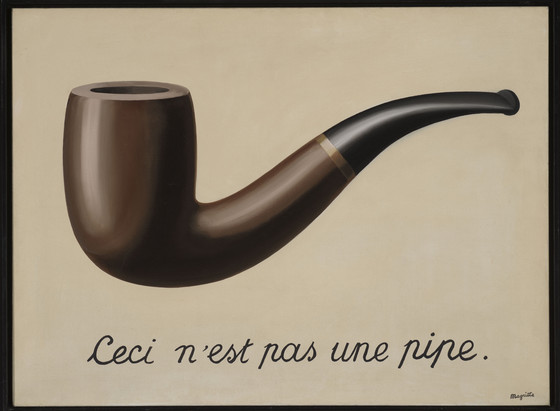
\includegraphics[width=0.7\linewidth]{images/Datenjudo/ma-150089-WEB} 

}

\caption{La trahison des images [Ceci n'est pas une pipe]}\label{fig:cecie-une-pipe}
\end{figure}

Hierbei ist gemeint, einen Datensatz sozusagen auf ein Fließband zu
legen und an jedem Arbeitsplatz einen Arbeitsschritt auszuführen. Der
springende Punkt ist, dass ein Dataframe als ``Rohstoff'' eingegeben
wird und jeder Arbeitsschritt seinerseits wieder einen Datafram
ausgiebt. Damit kann man sehr schön, einen ``Flow'' an Verarbeitung
erreichen, außerdem spart man sich Tipparbeit und die Syntax wird
lesbarer. Damit das Durchpfeifen funktioniert, benötigt man Befehle, die
als Eingabe einen Dataframe erwarten und wieder einen Dataframe
zurückliefern. Das Schaubild verdeutlich beispielhaft eine Abfolge des
Durchpfeifens (s. Abb. \ref{fig:fig-durchpfeifen}).

\begin{figure}

{\centering 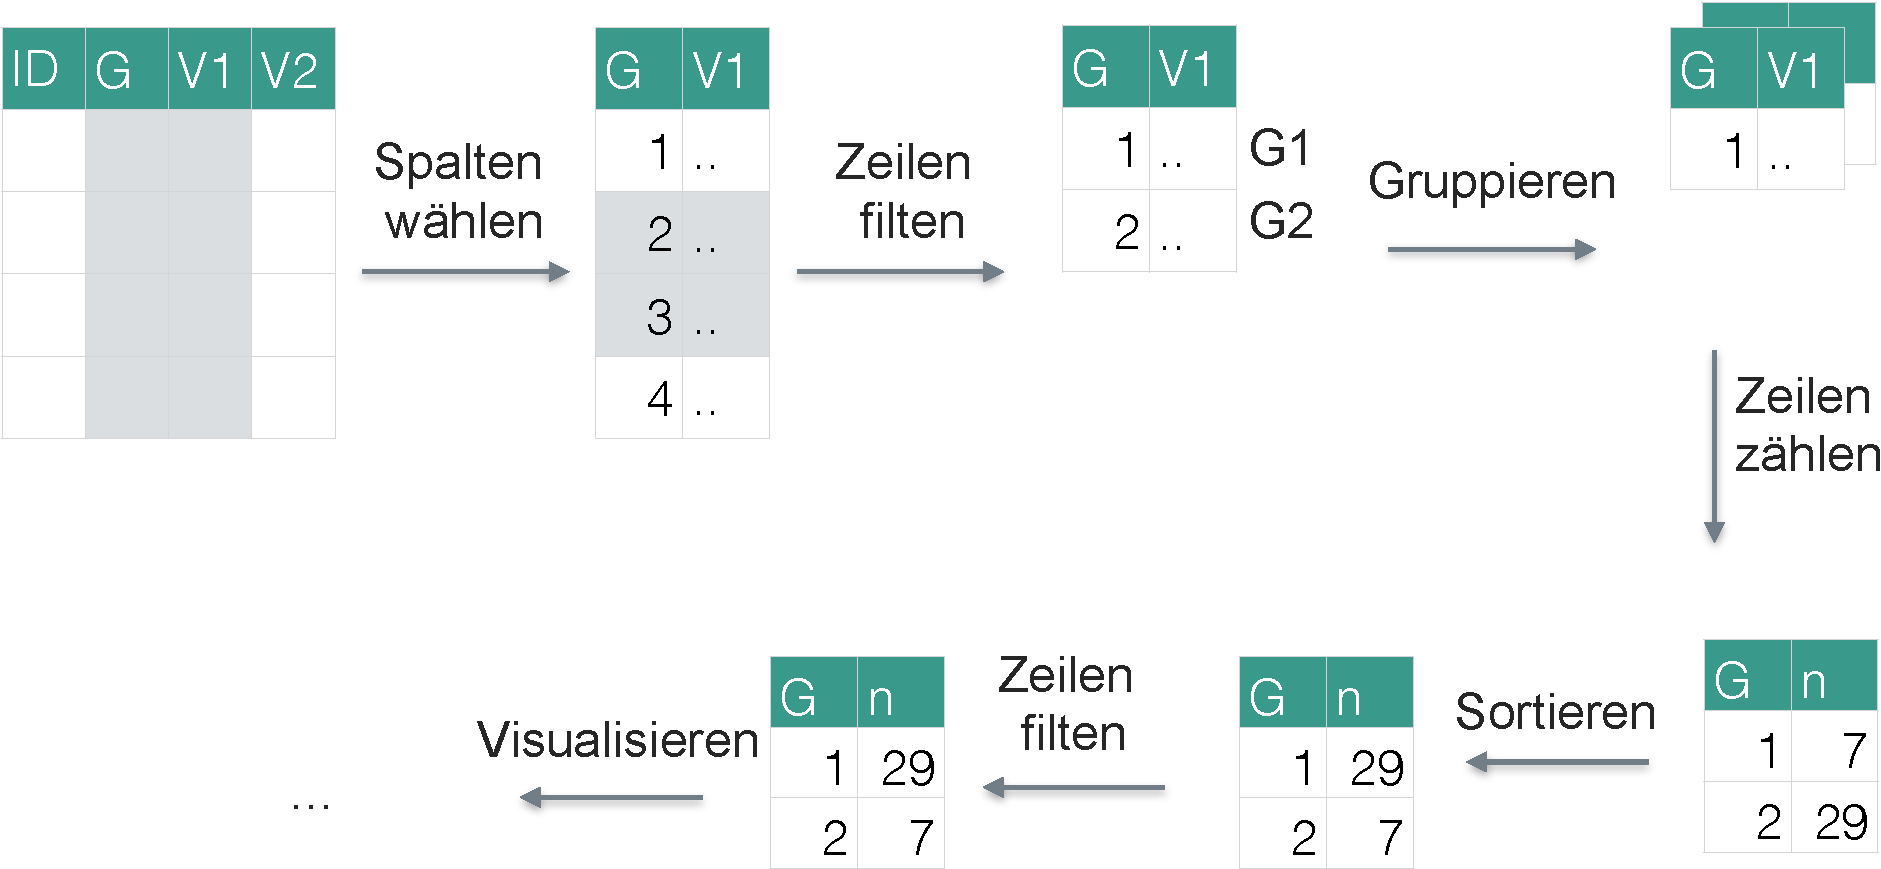
\includegraphics[width=0.8\linewidth]{images/Datenjudo/durchpfeifen} 

}

\caption{Das 'Durchpeifen'}\label{fig:fig-durchpfeifen}
\end{figure}

Die sog. ``Pfeife'' (pipe\index{Pfeife}: \texttt{\%\textgreater{}\%}) in
Anspielung an das berühmte Bild von René Magritte, verkettet Befehle
hintereinander. Das ist praktisch, da es die Syntax vereinfacht.
Vergleichen Sie mal diese Syntax

\begin{Shaded}
\begin{Highlighting}[]
\KeywordTok{filter}\NormalTok{(}\KeywordTok{summarise}\NormalTok{(}\KeywordTok{group_by}\NormalTok{(}\KeywordTok{filter}\NormalTok{(stats_test, }
       \NormalTok{!}\KeywordTok{is.na}\NormalTok{(score)), interest), }\DataTypeTok{mw =} \KeywordTok{mean}\NormalTok{(score)), mw >}\StringTok{ }\DecValTok{30}\NormalTok{)}
\end{Highlighting}
\end{Shaded}

mit dieser

\begin{Shaded}
\begin{Highlighting}[]
\NormalTok{stats_test %>%}\StringTok{ }
\StringTok{  }\KeywordTok{filter}\NormalTok{(!}\KeywordTok{is.na}\NormalTok{(score)) %>%}\StringTok{ }
\StringTok{  }\KeywordTok{group_by}\NormalTok{(interest) %>%}\StringTok{ }
\StringTok{  }\KeywordTok{summarise}\NormalTok{(}\DataTypeTok{mw =} \KeywordTok{mean}\NormalTok{(score)) %>%}\StringTok{ }
\StringTok{  }\KeywordTok{filter}\NormalTok{(mw >}\StringTok{ }\DecValTok{30}\NormalTok{)}
\CommentTok{#> # A tibble: 4 x 2}
\CommentTok{#>   interest    mw}
\CommentTok{#>      <int> <dbl>}
\CommentTok{#> 1        3  30.8}
\CommentTok{#> 2        5  32.5}
\CommentTok{#> 3        6  34.0}
\CommentTok{#> 4       NA  33.1}
\end{Highlighting}
\end{Shaded}

Die zweite ist viel einfacher! Lassen Sie uns die ``Pfeifen-Syntax'' in
deutschen Pseudo-Code zu übersetzen.

\BeginKnitrBlock{rmdpseudocode}
Nimm die Tabelle ``stats\_test'' UND DANN\\
filtere alle nicht-fehlenden Werte UND DANN\\
gruppiere die verbleibenden Werte nach ``interest'' UND DANN\\
bilde den Mittelwert (pro Gruppe) für ``score'' UND DANN\\
liefere nur die Werte größer als 30 zurück.
\EndKnitrBlock{rmdpseudocode}

Die zweite Syntax, in ``Pfeifenform'' ist viel einfacher zu verstehen
als die erste! Die erste Syntax ist verschachelt, man muss sie von innen
nach außen lesen. Das ist kompliziert. Die Pfeife in der 2. Syntax macht
es viel einfacher, die Snytax zu verstehen, da die Befehle
``hintereinander'' gestellt (sequenziell organisiert) sind.

Die Pfeife zerlegt die ``russische Puppe'', also ineinander
verschachelteten Code, in sequenzielle Schritte und zwar in der
richtigen Reihenfolge (entsprechend der Abarbeitung). Wir müssen den
Code nicht mehr von innen nach außen lesen (wie das bei einer
mathematischen Formel der Fall ist), sondern können wie bei einem
Kochrezept ``erstens \ldots{}, zweitens .., drittens \ldots{}'' lesen.
Die Pfeife macht die Syntax einfacher. Natürlich hätten wir die
verschachtelte Syntax in viele einzelne Befehle zerlegen können und
jeweils eine Zwischenergebnis speichern mit dem Zuweisungspfeil
\texttt{\textless{}-} und das Zwischenergebnis dann explizit an den
nächsten Befehl weitergeben. Eigentlich macht die Pfeife genau das - nur
mit weniger Tipparbeit. Und auch einfacher zu lesen. Flow!

\BeginKnitrBlock{rmdcaution}
Wenn Sie Befehle verketten mit der Pfeife, sind nur Befehle erlaubt, die
einen Datensatz als Eingabe verlangen und einen Datensatz ausgeben. Das
ist bei den hier vorgestellten Funktionen der Fall. Viele andere
Funktionen erfüllen dieses Kriterium aber nicht; in dem Fall liefert
\texttt{dplyr} eine Fehlermeldung.
\EndKnitrBlock{rmdcaution}

\subsection{\texorpdfstring{Spalten berechnen mit
\texttt{mutate}}{Spalten berechnen mit mutate}}\label{spalten-berechnen-mit-mutate}

Wenn man die Pfeife benutzt, ist der Befehl
\texttt{mutate}\index{dplyr::mutate} ganz praktisch: Er berechnet eine
Spalte. Normalerweise kann man einfach eine Spalte berechnen mit dem
Zuweisungsoperator:

Zum Beispiel so:

\begin{verbatim}
df$neue_spalte <- df$spalte1 + df$spalte2
\end{verbatim}

Innerhalb einer Pfeifen-Syntax geht das aber nicht (so gut). Da ist man
mit der Funtion \texttt{mutate} besser beraten; \texttt{mutate} leistest
just dasselbe wie die Pseudo-Syntax oben:

\begin{verbatim}
df %>% 
  mutate(neue_spalte = spalte1 + spalte2)
\end{verbatim}

In Worten:

\BeginKnitrBlock{rmdpseudocode}
Nimm die Tabelle ``df'' UND DANN\\
bilde eine neue Spalte mit dem Namen \texttt{neue\_spalte}, die sich
berechnet als Summe von \texttt{spalte1} und \texttt{spalte2}.
\EndKnitrBlock{rmdpseudocode}

Allerdings berücksichtigt \texttt{mutate} auch Gruppierungen. Der
Hauptvorteil ist die bessere Lesbarkeit durch Auflösen der
Verschachtelungen.

Ein konkretes Beispiel:

\begin{Shaded}
\begin{Highlighting}[]
\NormalTok{stats_test %>%}\StringTok{ }
\StringTok{  }\KeywordTok{mutate}\NormalTok{(}\DataTypeTok{bestanden =} \NormalTok{score >}\StringTok{ }\DecValTok{25}\NormalTok{) %>%}\StringTok{ }
\StringTok{  }\KeywordTok{head}\NormalTok{()}
\CommentTok{#> # A tibble: 6 x 7}
\CommentTok{#>   row_number           date_time study_time self_eval interest score}
\CommentTok{#>        <int>               <chr>      <int>     <int>    <int> <int>}
\CommentTok{#> 1          1 05.01.2017 13:57:01          5         8        5    29}
\CommentTok{#> 2          2 05.01.2017 21:07:56          3         7        3    29}
\CommentTok{#> 3          3 05.01.2017 23:33:47          5        10        6    40}
\CommentTok{#> 4          4 06.01.2017 09:58:05          2         3        2    18}
\CommentTok{#> 5          5 06.01.2017 14:13:08          4         8        6    34}
\CommentTok{#> 6          6 06.01.2017 14:21:18         NA        NA       NA    39}
\CommentTok{#> # ... with 1 more variables: bestanden <lgl>}
\end{Highlighting}
\end{Shaded}

Diese Syntax erzeugt eine neue Spalte innerhalb von
\texttt{stats\_test}; diese Spalte prüft pro Persion, ob \texttt{score}
\textgreater{} 25 ist. Falls ja (TRUE), dann ist \texttt{bestanden}
TRUE, ansonsten ist \texttt{bestanden} FALSE (Pech). \texttt{head} zeigt
die ersten 6 Zeilen des resultierenden Dataframes an.

Abb. \ref{fig:fig-mutate} zeigt Sinnbild für \texttt{mutate}:

\begin{figure}

{\centering 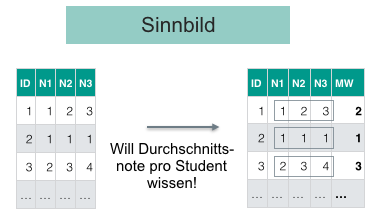
\includegraphics[width=0.7\linewidth]{images/Datenjudo/mutate} 

}

\caption{Sinnbild für mutate}\label{fig:fig-mutate}
\end{figure}

\subsection{Aufgaben}\label{aufgaben-9}

\begin{enumerate}
\def\labelenumi{\arabic{enumi}.}
\tightlist
\item
  Entschlüsseln Sie dieses Ungetüm! Übersetzen Sie diese Syntax auf
  Deutsch:
\end{enumerate}

\begin{Shaded}
\begin{Highlighting}[]

\KeywordTok{library}\NormalTok{(nycflights13)}
\KeywordTok{data}\NormalTok{(flights)}

\NormalTok{verspaetung <-}
\StringTok{  }\KeywordTok{filter}\NormalTok{(}
    \KeywordTok{summarise}\NormalTok{(}
    \KeywordTok{group_by}\NormalTok{(}\KeywordTok{filter}\NormalTok{(flights, !}\KeywordTok{is.na}\NormalTok{(dep_delay), month)), }
    \DataTypeTok{delay =} \KeywordTok{mean}\NormalTok{(dep_delay), }\DataTypeTok{n =} \KeywordTok{n}\NormalTok{()), n >}\StringTok{ }\DecValTok{10}\NormalTok{)}
 
\end{Highlighting}
\end{Shaded}

\begin{enumerate}
\def\labelenumi{\arabic{enumi}.}
\setcounter{enumi}{1}
\tightlist
\item
  Entschlüsseln Sie jetzt diese Syntax bzw. übersetzen Sie sie ins
  Deutsche:
\end{enumerate}

\begin{Shaded}
\begin{Highlighting}[]
\NormalTok{verspaetung <-}\StringTok{ }\NormalTok{flights %>%}\StringTok{ }\KeywordTok{filter}\NormalTok{(!}\KeywordTok{is.na}\NormalTok{(dep_delay)) %>%}
\KeywordTok{group_by}\NormalTok{(month) %>%}
\KeywordTok{summarise}\NormalTok{(}\DataTypeTok{delay =} \KeywordTok{mean}\NormalTok{(dep_delay), }\DataTypeTok{n =} \KeywordTok{n}\NormalTok{()) %>%}\StringTok{ }\KeywordTok{filter}\NormalTok{(n >}\StringTok{ }\DecValTok{10}\NormalTok{)}
\end{Highlighting}
\end{Shaded}

\begin{enumerate}
\def\labelenumi{\arabic{enumi}.}
\setcounter{enumi}{2}
\tightlist
\item
  (schwierig) Die Pfeife bei \texttt{arr\_delay}
\end{enumerate}

\begin{itemize}
\tightlist
\item
  Übersetzen Sie die folgende Pseudo-Syntax ins ERRRische!
\end{itemize}

\BeginKnitrBlock{rmdpseudocode}
Nehme den Datensatz \texttt{flights} UND DANN\ldots{}\\
Wähle daraus die Spalte \texttt{arr\_delay} UND DANN\ldots{}\\
Berechne den Mittelwert der Spalte UND DANN\ldots{}\\
ziehe vom Mittelwert die Spalte ab UND DANN\ldots{} quadriere die
einzelnen Differenzen UND DANN\ldots{} bilde davon den Mittelwert.
\EndKnitrBlock{rmdpseudocode}

Lösung:

\begin{Shaded}
\begin{Highlighting}[]
\NormalTok{flights %>%}\StringTok{ }
\StringTok{  }\KeywordTok{select}\NormalTok{(arr_delay) %>%}\StringTok{ }
\StringTok{  }\KeywordTok{mutate}\NormalTok{(}\DataTypeTok{arr_delay_delta =} \NormalTok{arr_delay -}\StringTok{ }\KeywordTok{mean}\NormalTok{(flights$arr_delay, }\DataTypeTok{na.rm =} \OtherTok{TRUE}\NormalTok{)) %>%}\StringTok{ }
\StringTok{  }\KeywordTok{mutate}\NormalTok{(}\DataTypeTok{arr_delay_delta_quadrat =} \NormalTok{arr_delay_delta^}\DecValTok{2}\NormalTok{) %>%}\StringTok{ }
\StringTok{  }\KeywordTok{summarise}\NormalTok{(}\DataTypeTok{arr_delay_var =} \KeywordTok{mean}\NormalTok{(arr_delay_delta_quadrat, }\DataTypeTok{na.rm =} \OtherTok{TRUE}\NormalTok{)) %>%}\StringTok{ }
\StringTok{  }\KeywordTok{summarise}\NormalTok{(}\KeywordTok{sqrt}\NormalTok{(arr_delay_var))}
\CommentTok{#> # A tibble: 1 x 1}
\CommentTok{#>   `sqrt(arr_delay_var)`}
\CommentTok{#>                   <dbl>}
\CommentTok{#> 1                  44.6}
\end{Highlighting}
\end{Shaded}

\begin{itemize}
\item
  Berechnen Sie die sd von \texttt{arr\_delay} in \texttt{flights}!
  Vergleichen Sie sie mit dem Ergebnis der vorherigen Aufgabe!\footnote{\texttt{sd(flights\$arr\_delay,\ na.rm\ =\ TRUE)}}
\item
  Was hat die Pfeifen-Syntax oben berechnet?\footnote{die sd von
    \texttt{arr\_delay}}
\end{itemize}

\section{Befehlsübersicht}\label{befehlsubersicht-2}

Tabelle \ref{tab:befehle-datenjudo} fasst die R-Funktionen dieses
Kapitels zusammen.

\begin{table}

\caption{\label{tab:befehle-datenjudo}Befehle des Kapitels 'Datenjudo'}
\centering
\begin{tabular}[t]{l|l}
\hline
Paket und Funktion & Beschreibung\\
\hline
dplyr::arrange & Sortiert Spalten\\
\hline
dplyr::filter & Filtert Zeilen\\
\hline
dplyr::select & Wählt Spalten\\
\hline
dplyr::group\_by & gruppiert einen Dataframe\\
\hline
dplyr::n & zählt Zeilen\\
\hline
dplyr::count & zählt Zeilen nach Untergruppen\\
\hline
\%>\% (dplyr) & verkettet Befehle\\
\hline
dplyr::mutate & erzeugt/berechnet Spalten\\
\hline
\end{tabular}
\end{table}

\section{Verweise}\label{verweise-2}

\begin{itemize}
\item
  Die offizielle Dokumentation von \texttt{dplyr} findet sich hier:
  \url{https://cran.r-project.org/web/packages/dplyr/dplyr.pdf}.
\item
  Eine schöne Demonstration der Mächtigkeit von \texttt{dplyr} findet
  sich hier: \url{http://bit.ly/2kX9lvC}.
\item
  Die GUI ``exploratory'' ist ein ``klickbare'' Umsetzung von
  \texttt{dplyr}, mächtig, modern und sieht cool aus:
  \url{https://exploratory.io}.
\item
  \emph{R for Data Science} bietet umfangreiche Unterstützung zu diesem
  Thema (Wickham und Grolemund \protect\hyperlink{ref-r4ds}{2016}).
\end{itemize}

\chapter{Praxisprobleme der
Datenaufbereitung}\label{praxisprobleme-der-datenaufbereitung}

\BeginKnitrBlock{rmdcaution}
Lernziele:

\begin{itemize}
\tightlist
\item
  Typische Probleme der Datenaufbereitung kennen.
\item
  Typische Probleme der Datenaufbereitung bearbeiten können.
\end{itemize}
\EndKnitrBlock{rmdcaution}

Laden wir zuerst die benötigten Pakete; v.a. ist das \texttt{dplyr} and
friends. Das geht mit dem Paket \texttt{tidyverse}.

\begin{Shaded}
\begin{Highlighting}[]
\KeywordTok{library}\NormalTok{(tidyverse)}
\KeywordTok{library}\NormalTok{(corrr)}
\KeywordTok{library}\NormalTok{(gridExtra)}
\KeywordTok{library}\NormalTok{(car)}
\end{Highlighting}
\end{Shaded}

Stellen wir einige typische Probleme des Datenjudo (genauer: der
Datenaufbereitung) zusammen. Probleme heißt hier nicht, dass es etwas
Schlimmes passiert ist, sondern es ist gemeint, wir schauen uns ein paar
typische Aufgabenstellungen an, die im Rahmen der Datenaufbereitung
häufig anfallen.

\section{Datenaufbereitung}\label{datenaufbereitung}

\subsection{Auf fehlende Werte prüfen}\label{auf-fehlende-werte-prufen}

Das geht recht einfach mit \texttt{summarise(mein\_dataframe)}. Der
Befehl liefert für jede Spalte des Dataframe \texttt{mein\_dataframe}
die Anzahl der fehlenden Werte zurück.

\begin{Shaded}
\begin{Highlighting}[]
\NormalTok{stats_test <-}\StringTok{ }\KeywordTok{read.csv}\NormalTok{(}\StringTok{"data/test_inf_short.csv"}\NormalTok{)}
\KeywordTok{summarise}\NormalTok{(stats_test)}
\CommentTok{#> data frame with 0 columns and 0 rows}
\end{Highlighting}
\end{Shaded}

\subsection{Fälle mit fehlenden Werte
löschen}\label{falle-mit-fehlenden-werte-loschen}

Weist eine Variable (Spalte) ``wenig'' fehlende Werte auf, so kann es
schlau sein, nichts zu tun. Eine andere Möglichkeit besteht darin, alle
entsprechenden Zeilen zu löschen. Man sollte aber schauen, wie viele
Zeilen dadurch verloren gehen.

\begin{Shaded}
\begin{Highlighting}[]
\CommentTok{# Unsprünglich Anzahl an Fällen (Zeilen)}
\KeywordTok{nrow}\NormalTok{(stats_test)}
\CommentTok{#> [1] 306}

\CommentTok{# Nach Umwandlung in neuen Dataframe}
\NormalTok{stats_test %>%}
\StringTok{   }\NormalTok{na.omit ->}\StringTok{ }\NormalTok{stats_test_na_omit}
\KeywordTok{nrow}\NormalTok{(stats_test_na_omit)}
\CommentTok{#> [1] 238}

\CommentTok{# Nur die Anzahl der bereinigten Daten}
\NormalTok{stats_test %>%}
\StringTok{   }\NormalTok{na.omit %>%}
\StringTok{   }\NormalTok{nrow}
\CommentTok{#> [1] 238}
\end{Highlighting}
\end{Shaded}

\BeginKnitrBlock{rmdcaution}
Bei mit der Pfeife verketteten Befehlen darf man für Funktionen die
runden Klammern weglassen, wenn man keinen Parameter schreibt. Also ist
\texttt{nrow} (ohne Klammern) erlaubt bei \texttt{dplyr}, wo es
eigentlich \texttt{nrow()} heißen müsste. Sie dürfen die Klammern
natürlich schreiben, aber sie müssen nicht.
\EndKnitrBlock{rmdcaution}

Hier verlieren wir 68 Zeilen, das verschmerzen wir. Welche Zeilen
verlieren wir eigentlich?

\begin{Shaded}
\begin{Highlighting}[]
\NormalTok{stats_test %>%}\StringTok{ }
\StringTok{   }\KeywordTok{filter}\NormalTok{(!}\KeywordTok{complete.cases}\NormalTok{(.))  }\CommentTok{# Nur die nicht-kompletten Fälle filtern}
\CommentTok{#>    row_number           date_time study_time self_eval interest score}
\CommentTok{#> 1           6 06.01.2017 14:21:18         NA        NA       NA    39}
\CommentTok{#> 2           7 06.01.2017 14:25:49         NA        NA       NA    40}
\CommentTok{#> 3          15 09.01.2017 15:23:15         NA        NA       NA    30}
\CommentTok{#> 4          19 10.01.2017 17:16:48         NA        NA       NA    22}
\CommentTok{#> 5          42 13.01.2017 14:08:08         NA        NA       NA    38}
\CommentTok{#> 6          49 14.01.2017 07:02:39         NA        NA       NA    39}
\CommentTok{#> 7          67 15.01.2017 13:30:48         NA        NA       NA    24}
\CommentTok{#> 8          74 15.01.2017 16:12:54         NA        NA       NA    30}
\CommentTok{#> 9          83 16.01.2017 10:16:52         NA        NA       NA    40}
\CommentTok{#> 10         89 16.01.2017 21:18:05         NA        NA       NA    34}
\CommentTok{#> 11         91 17.01.2017 15:19:36         NA        NA       NA    29}
\CommentTok{#> 12         99 18.01.2017 09:04:30         NA        NA       NA    37}
\CommentTok{#> 13        104 18.01.2017 13:42:20         NA        NA       NA    39}
\CommentTok{#> 14        106 18.01.2017 15:52:04         NA        NA       NA    38}
\CommentTok{#> 15        111 18.01.2017 19:24:49         NA        NA       NA    37}
\CommentTok{#> 16        117 19.01.2017 08:06:05         NA        NA       NA    37}
\CommentTok{#> 17        118 19.01.2017 08:54:43         NA        NA       NA    33}
\CommentTok{#> 18        119 19.01.2017 09:05:01         NA        NA       NA    40}
\CommentTok{#> 19        124 19.01.2017 12:51:10         NA        NA       NA    32}
\CommentTok{#> 20        125 19.01.2017 13:03:26         NA        NA       NA    30}
\CommentTok{#> 21        132 19.01.2017 18:22:32         NA        NA       NA    40}
\CommentTok{#> 22        133 19.01.2017 18:22:38         NA        NA       NA    38}
\CommentTok{#> 23        139 19.01.2017 18:35:56         NA        NA       NA    31}
\CommentTok{#> 24        141 19.01.2017 18:44:32         NA        NA       NA    34}
\CommentTok{#> 25        150 20.01.2017 09:53:47         NA        NA       NA    32}
\CommentTok{#> 26        155 20.01.2017 15:33:55         NA        NA       NA    39}
\CommentTok{#> 27        157 20.01.2017 17:34:48         NA        NA       NA    31}
\CommentTok{#> 28        158 20.01.2017 17:53:16         NA        NA       NA    36}
\CommentTok{#> 29        159 20.01.2017 17:57:26         NA        NA       NA    34}
\CommentTok{#> 30        160 20.01.2017 17:59:19         NA        NA       NA    34}
\CommentTok{#> 31        162 20.01.2017 18:00:53         NA        NA       NA    35}
\CommentTok{#> 32        163 20.01.2017 18:04:21         NA        NA       NA    36}
\CommentTok{#> 33        180 21.01.2017 08:04:17         NA        NA       NA    39}
\CommentTok{#> 34        183 21.01.2017 12:20:37         NA        NA       NA    31}
\CommentTok{#> 35        187 21.01.2017 16:27:32         NA        NA       NA    26}
\CommentTok{#> 36        191 22.01.2017 11:31:27         NA        NA       NA    36}
\CommentTok{#> 37        195 22.01.2017 13:24:51         NA        NA       NA    23}
\CommentTok{#> 38        202 22.01.2017 17:13:02         NA        NA       NA    36}
\CommentTok{#> 39        206 22.01.2017 18:42:49         NA        NA       NA    20}
\CommentTok{#> 40        207 22.01.2017 18:56:56         NA        NA       NA    28}
\CommentTok{#> 41        211 22.01.2017 20:28:43         NA        NA       NA    38}
\CommentTok{#> 42        213 22.01.2017 21:47:06         NA        NA       NA    29}
\CommentTok{#> 43        225 23.01.2017 13:24:22         NA        NA       NA    39}
\CommentTok{#> 44        226 23.01.2017 14:17:10         NA        NA       NA    36}
\CommentTok{#> 45        235 23.01.2017 18:26:20         NA        NA       NA    20}
\CommentTok{#> 46        238 23.01.2017 19:53:10         NA        NA       NA    27}
\CommentTok{#> 47        242 24.01.2017 14:09:33         NA        NA       NA    28}
\CommentTok{#> 48        245 24.01.2017 14:56:24         NA        NA       NA    28}
\CommentTok{#> 49        246 24.01.2017 15:09:44         NA        NA       NA    24}
\CommentTok{#> 50        247 24.01.2017 15:37:27         NA        NA       NA    28}
\CommentTok{#> 51        249 24.01.2017 17:19:54         NA        NA       NA    40}
\CommentTok{#> 52        253 25.01.2017 09:32:55         NA        NA       NA    39}
\CommentTok{#> 53        255 25.01.2017 10:05:00         NA        NA       NA    29}
\CommentTok{#> 54        265 25.01.2017 13:14:00         NA        NA       NA    30}
\CommentTok{#> 55        270 25.01.2017 16:35:41         NA        NA       NA    28}
\CommentTok{#> 56        271 25.01.2017 16:53:17         NA        NA       NA    34}
\CommentTok{#> 57        272 25.01.2017 17:03:21         NA        NA       NA    36}
\CommentTok{#> 58        274 25.01.2017 17:38:36         NA        NA       NA    37}
\CommentTok{#> 59        275 25.01.2017 18:06:36         NA        NA       NA    34}
\CommentTok{#> 60        283 26.01.2017 10:39:44         NA        NA       NA    23}
\CommentTok{#> 61        285 26.01.2017 10:54:41         NA        NA       NA    34}
\CommentTok{#> 62        286 26.01.2017 11:19:10         NA        NA       NA    38}
\CommentTok{#> 63        288 26.01.2017 13:36:14         NA        NA       NA    28}
\CommentTok{#> 64        289 26.01.2017 14:19:14         NA        NA       NA    31}
\CommentTok{#> 65        290 26.01.2017 14:34:23         NA        NA       NA    36}
\CommentTok{#> 66        291 26.01.2017 14:55:17         NA        NA       NA    39}
\CommentTok{#> 67        293 26.01.2017 15:17:47         NA        NA       NA    36}
\CommentTok{#> 68        294 26.01.2017 15:51:56         NA        NA       NA    34}
\end{Highlighting}
\end{Shaded}

Man beachte, dass der Punkt \texttt{.} für den Datensatz steht, wie er
vom letzten Schritt weitergegeben wurde. Innerhalb einer
dplyr-Befehls-Kette können wir den Datensatz, wie er im letzten Schritt
beschaffen war, stets mit \texttt{.} ansprechen; ganz praktisch, weil
schnell zu tippen. Natürlich könnten wir diesen Datensatz jetzt als
neues Objekt speichern und damit weiter arbeiten. Das Ausrufezeichen
\texttt{!} steht für logisches ``Nicht''.

In Pseudo-Syntax liest es sich so:

\BeginKnitrBlock{rmdpseudocode}
Nehme den Datensatz \texttt{stats\_test} UND DANN\ldots{}\\
filtere die nicht-kompletten Fälle
\EndKnitrBlock{rmdpseudocode}

\subsection{Fehlende Werte ggf.
ersetzen}\label{fehlende-werte-ggf.-ersetzen}

Ist die Anzahl der fehlenden Werte zu groß, als dass wir es verkraften
könnten, die Zeilen zu löschen, so können wir die fehlenden Werte
ersetzen. Allein, das ist ein weites Feld und übersteigt den Anspruch
dieses Kurses\footnote{Das sagen Autoren, wenn sie nicht genau wissen,
  wie etwas funktioniert.}. Eine einfache, aber nicht die beste
Möglichkeit, besteht darin, die fehlenden Werte durch einen
repräsentativen Wert, z.B. den Mittelwert der Spalte, zu ersetzen.

\begin{Shaded}
\begin{Highlighting}[]
\NormalTok{stats_test$interest <-}\StringTok{ }\KeywordTok{replace}\NormalTok{(stats_test$interest, }\KeywordTok{is.na}\NormalTok{(stats_test$interest),}
                         \KeywordTok{mean}\NormalTok{(stats_test$interest, }\DataTypeTok{na.rm =} \OtherTok{TRUE}\NormalTok{))}

\KeywordTok{sum}\NormalTok{(}\KeywordTok{is.na}\NormalTok{(stats_test$interest))}
\CommentTok{#> [1] 0}
\end{Highlighting}
\end{Shaded}

\texttt{replace}\footnote{aus dem ``Standard-R'', d.h. Paket ``base''.}
ersetzt Werte aus dem Vektor \texttt{stats\_test\$interest} alle Werte,
für die \texttt{is.na(stats\_test\$interest)} wahr ist, bei Zeilen mit
fehlenden Werten in dieser Spalte also. Diese Werte werden durch den
Mittelwert der Spalte ersetzt\footnote{Hier findet sich eine
  ausführlichere Darstellung:
  \url{https://sebastiansauer.github.io/checklist_data_cleansing/index.html}}.

\subsection{Nach Fehlern suchen}\label{nach-fehlern-suchen}

Leicht schleichen sich Tippfehler oder andere Fehler ein. Man sollte
darauf prüfen; so könnte man sich ein Histogramm ausgeben lassen pro
Variable, um ``ungewöhnliche'' Werte gut zu erkennen. Meist geht das
besser als durch das reine Betrachten von Zahlen. Gibt es wenig
unterschiedliche Werte, so kann man sich auch die unterschiedlichen
Werte ausgeben lassen.

\begin{Shaded}
\begin{Highlighting}[]
\NormalTok{stats_test %>%}\StringTok{ }
\StringTok{  }\KeywordTok{count}\NormalTok{(interest) }
\CommentTok{#> # A tibble: 7 x 2}
\CommentTok{#>   interest     n}
\CommentTok{#>      <dbl> <int>}
\CommentTok{#> 1     1.00    30}
\CommentTok{#> 2     2.00    47}
\CommentTok{#> 3     3.00    66}
\CommentTok{#> 4     3.21    68}
\CommentTok{#> 5     4.00    41}
\CommentTok{#> 6     5.00    45}
\CommentTok{#> 7     6.00     9}
\end{Highlighting}
\end{Shaded}

Da in der Umfrage nur ganze Zahlen von 1 bis 5 abgefragt wurden, ist die
\texttt{3.21...} auf den ersten Blick suspekt. In diesem Fall ist aber
alles ok, da wir diesen Wert selber erzeugt haben.

\subsection{Ausreißer identifizieren}\label{ausreier-identifizieren}

Ähnlich zu Fehlern, steht man Ausreißer häufig skeptisch gegenüber.
Allerdings kann man nicht pauschal sagen, das Extremwerte entfernt
werden sollen: Vielleicht war jemand in der Stichprobe wirklich nur
1.20m groß? Hier gilt es, begründet und nachvollziehbar im Einzelfall zu
entscheiden. Histogramme und Boxplots sind wieder ein geeignetes Mittel,
um Ausreißer zu finden (vgl. Abb. \ref{fig:fig-ausreisser}).

\begin{Shaded}
\begin{Highlighting}[]
\KeywordTok{qplot}\NormalTok{(}\DataTypeTok{x =} \NormalTok{score, }\DataTypeTok{data =} \NormalTok{stats_test, }\DataTypeTok{binwidth =} \DecValTok{1}\NormalTok{)}
\end{Highlighting}
\end{Shaded}

\begin{figure}

{\centering 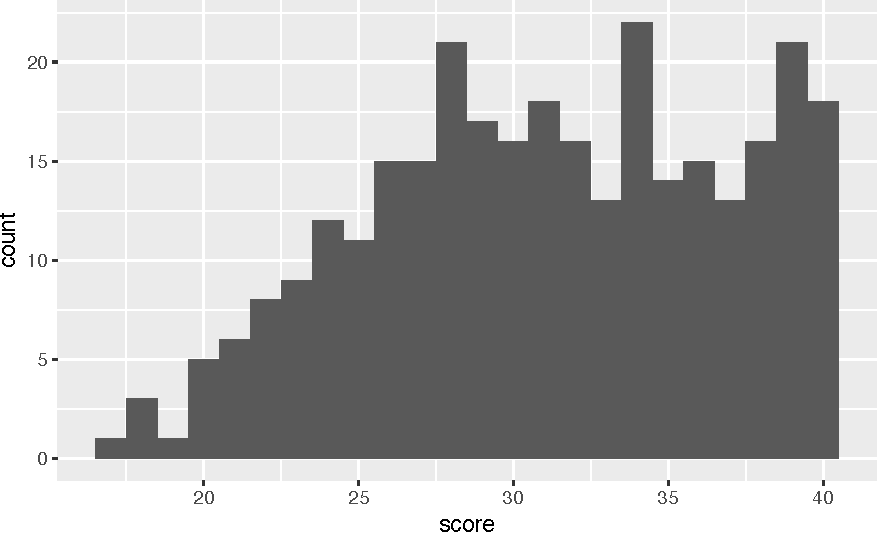
\includegraphics[width=0.7\linewidth]{043_Typische_Probleme_Datenanalyse_files/figure-latex/fig-ausreisser-1} 

}

\caption{Ausreißer identifizieren}\label{fig:fig-ausreisser}
\end{figure}

Mit \texttt{binwidth\ =\ 1} sagen wir, dass jeder Balken (bin) eine
Breite (width) von 1 haben soll.

\subsection{Hochkorrelierte Variablen
finden}\label{hochkorrelierte-variablen-finden}

Haben zwei Leute die gleiche Meinung, so ist einer von beiden
überflüssig - wird behauptet. Ähnlich bei Variablen; sind zwei Variablen
sehr hoch korreliert (\textgreater{}.9, als grober (!) Richtwert), so
bringt die zweite kaum Informationszuwachs zur ersten. Und kann z.B.
ausgeschlossen werden.

Nehmen wir dazu den Datensatz \texttt{extra} her.

\begin{Shaded}
\begin{Highlighting}[]
\NormalTok{extra <-}\StringTok{ }\KeywordTok{read.csv}\NormalTok{(}\StringTok{"data/extra.csv"}\NormalTok{)}
\end{Highlighting}
\end{Shaded}

\begin{Shaded}
\begin{Highlighting}[]
\NormalTok{extra %>%}\StringTok{ }
\StringTok{  }\KeywordTok{select}\NormalTok{(i01:i10) %>%}\StringTok{ }\CommentTok{# Wähle die Variablen von i01 bis i10 aus}
\StringTok{  }\KeywordTok{correlate}\NormalTok{() ->}\StringTok{ }\NormalTok{km   }\CommentTok{# Korrelationsmatrix berechnen}
\NormalTok{km  }
\CommentTok{#> # A tibble: 10 x 11}
\CommentTok{#>    rowname    i01   i02r    i03    i04    i05  i06r   i07   i08    i09}
\CommentTok{#>      <chr>  <dbl>  <dbl>  <dbl>  <dbl>  <dbl> <dbl> <dbl> <dbl>  <dbl>}
\CommentTok{#>  1     i01     NA 0.4895 0.0805 0.4528 0.4481 0.450 0.309 0.387 0.3795}
\CommentTok{#>  2    i02r 0.4895     NA 0.0849 0.3603 0.3897 0.520 0.240 0.323 0.2730}
\CommentTok{#>  3     i03 0.0805 0.0849     NA 0.0323 0.0492 0.155 0.156 0.101 0.0211}
\CommentTok{#>  4     i04 0.4528 0.3603 0.0323     NA 0.6478 0.316 0.446 0.219 0.2472}
\CommentTok{#>  5     i05 0.4481 0.3897 0.0492 0.6478     NA 0.348 0.395 0.287 0.2983}
\CommentTok{#>  6    i06r 0.4504 0.5197 0.1554 0.3163 0.3482    NA 0.163 0.294 0.2937}
\CommentTok{#>  7     i07 0.3090 0.2396 0.1557 0.4459 0.3949 0.163    NA 0.317 0.2803}
\CommentTok{#>  8     i08 0.3873 0.3232 0.1006 0.2190 0.2875 0.294 0.317    NA 0.4095}
\CommentTok{#>  9     i09 0.3795 0.2730 0.0211 0.2472 0.2983 0.294 0.280 0.409     NA}
\CommentTok{#> 10     i10 0.1850 0.0789 0.0939 0.3520 0.2929 0.136 0.380 0.220 0.1552}
\CommentTok{#> # ... with 1 more variables: i10 <dbl>}
\end{Highlighting}
\end{Shaded}

In diesem Beispiel sind keine Variablen sehr hoch korreliert. Wir leiten
keine weiteren Schritte ein, abgesehen von einer Visualisierung.

\begin{Shaded}
\begin{Highlighting}[]

\NormalTok{km %>%}\StringTok{ }
\StringTok{  }\KeywordTok{shave}\NormalTok{() %>%}\StringTok{ }\CommentTok{# Oberes Dreieck ist redundant, wird "abrasiert"}
\StringTok{  }\KeywordTok{rplot}\NormalTok{()  }\CommentTok{# Korrelationsplot}
\end{Highlighting}
\end{Shaded}

\begin{figure}

{\centering 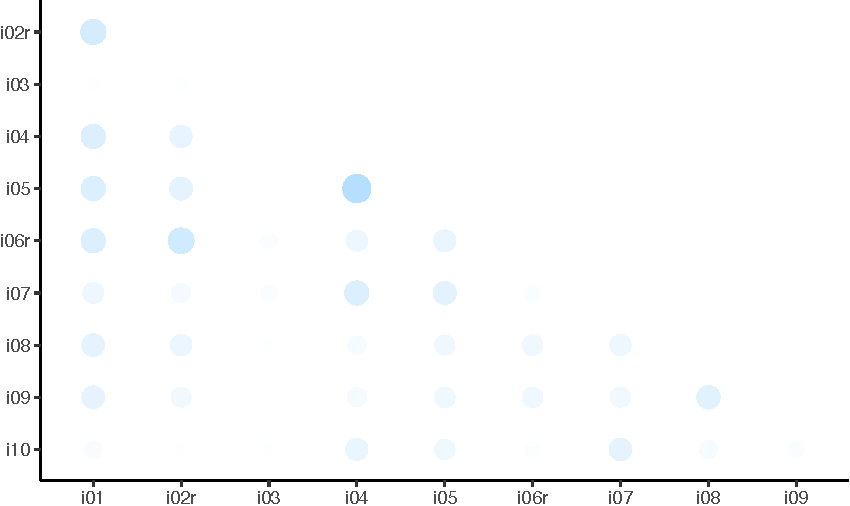
\includegraphics[width=0.7\linewidth]{043_Typische_Probleme_Datenanalyse_files/figure-latex/fig-corrr-1} 

}

\caption{Ein Korrelationsplot}\label{fig:fig-corrr}
\end{figure}

Die Funktion \texttt{correlate} stammt aus dem Paket
\texttt{corrr}\footnote{\url{https://github.com/drsimonj/corrr}},
welches vorher installiert und geladen sein muss. Hier ist die
Korrelation nicht zu groß, so dass wir keine weiteren Schritte
unternehmen. Hätten wir eine sehr hohe Korrelation gefunden, so hätten
wir eine der beiden beteiligten Variablen aus dem Datensatz löschen
können.

\subsection{z-Standardisieren}\label{z-standardisieren}

Für eine Reihe von Analysen ist es wichtig, die Skalierung der Variablen
zur vereinheitlichen. Die z-Standardisierung ist ein übliches Vorgehen.
Dabei wird der Mittelwert auf 0 transformiert und die SD auf 1; man
spricht - im Falle von (hinreichend) normalverteilten Variablen - jetzt
von der \emph{Standardnormalverteilung}\index{Standardnormalverteilung}.
Unterscheiden sich zwei Objekte A und B in einer
standardnormalverteilten Variablen, so sagt dies nur etwas zur relativen
Position von A zu B innerhalb ihrer Verteilung aus - im Gegensatz zu den
Rohwerten.

\begin{Shaded}
\begin{Highlighting}[]
\NormalTok{extra %>%}\StringTok{ }
\StringTok{  }\KeywordTok{select_if}\NormalTok{(is.numeric) %>%}\StringTok{  }\CommentTok{# Spalte nur auswählen, wenn numerisch}
\StringTok{  }\KeywordTok{scale}\NormalTok{() %>%}\StringTok{  }\CommentTok{# z-standardisieren}
\StringTok{  }\KeywordTok{head}\NormalTok{()  }\CommentTok{# nur die ersten paar Zeilen abdrucken}
\CommentTok{#>          X    i01  i02r     i03   i04     i05    i06r     i07     i08  i09}
\CommentTok{#> [1,] -1.73 -0.499 -0.15  1.1784 -0.33  1.2307  1.3643  0.0466 -1.0826 -0.5}
\CommentTok{#> [2,] -1.72 -1.964 -1.39 -0.9838 -1.70 -0.0705 -1.2193 -1.3192  0.0867 -0.5}
\CommentTok{#> [3,] -1.71 -0.499  1.09 -0.9838  1.04  1.2307 -2.5111  0.0466 -1.0826 -0.5}
\CommentTok{#> [4,] -1.71 -0.499 -0.15  0.0973  1.04 -0.0705  0.0725  0.0466  0.0867 -0.5}
\CommentTok{#> [5,] -1.70  0.966 -0.15 -0.9838  1.04  1.2307  0.0725  1.4124 -1.0826 -0.5}
\CommentTok{#> [6,] -1.69 -0.499 -1.39 -0.9838  1.04 -1.3718  0.0725  1.4124  0.0867 -0.5}
\CommentTok{#>         i10 n_facebook_friends n_hangover    age extra_single_item}
\CommentTok{#> [1,] -1.388            -0.4111     -0.434 -0.306             1.350}
\CommentTok{#> [2,] -1.388            -0.9094     -0.487  1.621             0.183}
\CommentTok{#> [3,] -1.388            -0.5322     -0.487 -0.131             1.350}
\CommentTok{#> [4,] -0.273            -0.5841      0.305  2.322             0.183}
\CommentTok{#> [5,]  1.956            -0.9301     -0.487  0.570             1.350}
\CommentTok{#> [6,]  0.841             0.0249     -0.434  1.271             1.350}
\CommentTok{#>      time_conversation n_party extra_description prop_na_per_row}
\CommentTok{#> [1,]           -0.0468  0.0961                NA           0.519}
\CommentTok{#> [2,]           -0.0468 -0.6174                NA           0.519}
\CommentTok{#> [3,]           -0.0468 -0.7126                NA           0.519}
\CommentTok{#> [4,]           -0.0468  0.3340                NA           0.519}
\CommentTok{#> [5,]           -0.0468 -0.6650                NA           0.519}
\CommentTok{#> [6,]           -0.0468 -0.6650                NA           0.519}
\CommentTok{#>      extra_mean extra_median client_freq}
\CommentTok{#> [1,]    -0.0175       -0.024          NA}
\CommentTok{#> [2,]    -1.7517       -1.740          NA}
\CommentTok{#> [3,]    -0.6678       -0.024          NA}
\CommentTok{#> [4,]    -0.0175       -0.024          NA}
\CommentTok{#> [5,]     0.6328        0.834          NA}
\CommentTok{#> [6,]    -0.2343       -0.024          NA}
\end{Highlighting}
\end{Shaded}

Dieser Befehl liefert zwei z-standardisierte Spalten zurück. Kommoder
ist es aber, alle Spalten des Datensatzes zurück zu bekommen, wobei
zusätzlich die z-Werte aller numerischen Variablen hinzugekommen sind:

\begin{Shaded}
\begin{Highlighting}[]
\NormalTok{extra %>%}\StringTok{ }
\StringTok{  }\KeywordTok{mutate_if}\NormalTok{(is.numeric, }\KeywordTok{funs}\NormalTok{(}\StringTok{"z"} \NormalTok{=}\StringTok{ }\NormalTok{scale)) %>%}\StringTok{ }
\StringTok{  }\NormalTok{head}
\CommentTok{#>   X           timestamp code i01 i02r i03 i04 i05 i06r i07 i08 i09 i10}
\CommentTok{#> 1 1 11.03.2015 19:17:48  HSC   3    3   3   3   4    4   3   2   3   1}
\CommentTok{#> 2 2 11.03.2015 19:18:05  ERB   2    2   1   2   3    2   2   3   3   1}
\CommentTok{#> 3 3 11.03.2015 19:18:09  ADP   3    4   1   4   4    1   3   2   3   1}
\CommentTok{#> 4 4 11.03.2015 19:18:19  KHB   3    3   2   4   3    3   3   3   3   2}
\CommentTok{#> 5 5 11.03.2015 19:18:19  PTG   4    3   1   4   4    3   4   2   3   4}
\CommentTok{#> 6 6 11.03.2015 19:18:23  ABL   3    2   1   4   2    3   4   3   3   3}
\CommentTok{#>   n_facebook_friends n_hangover age  sex extra_single_item}
\CommentTok{#> 1                250          1  24 Frau                 4}
\CommentTok{#> 2                106          0  35 Frau                 3}
\CommentTok{#> 3                215          0  25 Frau                 4}
\CommentTok{#> 4                200         15  39 Frau                 3}
\CommentTok{#> 5                100          0  29 Frau                 4}
\CommentTok{#> 6                376          1  33 Mann                 4}
\CommentTok{#>   time_conversation presentation n_party clients extra_vignette}
\CommentTok{#> 1                10         nein      20                       }
\CommentTok{#> 2                15         nein       5                       }
\CommentTok{#> 3                15         nein       3                       }
\CommentTok{#> 4                 5         nein      25                       }
\CommentTok{#> 5                 5         nein       4                       }
\CommentTok{#> 6                20           ja       4                       }
\CommentTok{#>   extra_description prop_na_per_row extra_mean extra_median client_freq}
\CommentTok{#> 1                NA          0.0435        2.9          3.0          NA}
\CommentTok{#> 2                NA          0.0435        2.1          2.0          NA}
\CommentTok{#> 3                NA          0.0435        2.6          3.0          NA}
\CommentTok{#> 4                NA          0.0435        2.9          3.0          NA}
\CommentTok{#> 5                NA          0.0435        3.2          3.5          NA}
\CommentTok{#> 6                NA          0.0435        2.8          3.0          NA}
\CommentTok{#>     X_z  i01_z i02r_z   i03_z i04_z   i05_z  i06r_z   i07_z   i08_z i09_z}
\CommentTok{#> 1 -1.73 -0.499  -0.15  1.1784 -0.33  1.2307  1.3643  0.0466 -1.0826  -0.5}
\CommentTok{#> 2 -1.72 -1.964  -1.39 -0.9838 -1.70 -0.0705 -1.2193 -1.3192  0.0867  -0.5}
\CommentTok{#> 3 -1.71 -0.499   1.09 -0.9838  1.04  1.2307 -2.5111  0.0466 -1.0826  -0.5}
\CommentTok{#> 4 -1.71 -0.499  -0.15  0.0973  1.04 -0.0705  0.0725  0.0466  0.0867  -0.5}
\CommentTok{#> 5 -1.70  0.966  -0.15 -0.9838  1.04  1.2307  0.0725  1.4124 -1.0826  -0.5}
\CommentTok{#> 6 -1.69 -0.499  -1.39 -0.9838  1.04 -1.3718  0.0725  1.4124  0.0867  -0.5}
\CommentTok{#>    i10_z n_facebook_friends_z n_hangover_z  age_z extra_single_item_z}
\CommentTok{#> 1 -1.388              -0.4111       -0.434 -0.306               1.350}
\CommentTok{#> 2 -1.388              -0.9094       -0.487  1.621               0.183}
\CommentTok{#> 3 -1.388              -0.5322       -0.487 -0.131               1.350}
\CommentTok{#> 4 -0.273              -0.5841        0.305  2.322               0.183}
\CommentTok{#> 5  1.956              -0.9301       -0.487  0.570               1.350}
\CommentTok{#> 6  0.841               0.0249       -0.434  1.271               1.350}
\CommentTok{#>   time_conversation_z n_party_z extra_description_z prop_na_per_row_z}
\CommentTok{#> 1             -0.0468    0.0961                  NA             0.519}
\CommentTok{#> 2             -0.0468   -0.6174                  NA             0.519}
\CommentTok{#> 3             -0.0468   -0.7126                  NA             0.519}
\CommentTok{#> 4             -0.0468    0.3340                  NA             0.519}
\CommentTok{#> 5             -0.0468   -0.6650                  NA             0.519}
\CommentTok{#> 6             -0.0468   -0.6650                  NA             0.519}
\CommentTok{#>   extra_mean_z extra_median_z client_freq_z}
\CommentTok{#> 1      -0.0175         -0.024            NA}
\CommentTok{#> 2      -1.7517         -1.740            NA}
\CommentTok{#> 3      -0.6678         -0.024            NA}
\CommentTok{#> 4      -0.0175         -0.024            NA}
\CommentTok{#> 5       0.6328          0.834            NA}
\CommentTok{#> 6      -0.2343         -0.024            NA}
\end{Highlighting}
\end{Shaded}

Der Befehl \texttt{mutate} berechnet eine neue Spalte;
\texttt{mutate\_if} tut dies, wenn die Spalte numerisch ist. Die neue
Spalte wird berechnet als z-Transformierung der alten Spalte; zum
Spaltenname wird ein ``\_z" hinzugefügt. Natürlich hätten wir auch mit
\texttt{select} ``händisch'' die relevanten Spalten auswählen können.

\subsection{Quasi-Konstante finden}\label{quasi-konstante-finden}

Hier suchen wir nach Variablen (Spalten), die nur einen Wert oder
zumindest nur sehr wenige verschiedene Werte aufweisen. Oder, ähnlich:
Wenn 99.9\% der Fälle nur von einem Wert bestritten wird. In diesen
Fällen kann man die Variable als ``Quasi-Konstante'' bezeichnen.
Quasi-Konstanten sind für die Modellierung von keiner oder nur geringer
Bedeutung; sie können in der Regel für weitere Analysen ausgeschlossen
werden.

Haben wir z.B. nur Männer im Datensatz, so kann das Geschlecht nicht für
Unterschiede im Einkommen verantwortlich sein. Besser ist es, die
Variable Geschlecht zu entfernen. Auch hier sind Histogramme oder
Boxplots von Nutzen zur Identifikation von (Quasi-)Konstanten.
Alternativ kann man sich auch pro die Streuung (numerische Variablen)
oder die Anzahl unterschiedlicher Werte (qualitative Variablen) ausgeben
lassen:

\begin{Shaded}
\begin{Highlighting}[]
\KeywordTok{IQR}\NormalTok{(extra$n_facebook_friends, }\DataTypeTok{na.rm =} \OtherTok{TRUE}\NormalTok{)  }\CommentTok{# keine Konstante}
\CommentTok{#> [1] 288}
\KeywordTok{n_distinct}\NormalTok{(extra$sex)  }\CommentTok{# es scheint 3 Geschlechter zu geben...}
\CommentTok{#> [1] 3}
\end{Highlighting}
\end{Shaded}

\subsection{Auf Normalverteilung
prüfen}\label{auf-normalverteilung-prufen}

Einige statistische Verfahren gehen von normalverteilten Variablen aus,
daher macht es Sinn, Normalverteilung zu prüfen. \emph{Perfekte}
Normalverteilung ist genau so häufig wie \emph{perfekte} Kreise in der
Natur. Entsprechend werden Signifikanztests, die ja auf perfekte
Normalverteilung prüfen, \emph{immer signifikant} sein, sofern die
\emph{Stichprobe groß} genug ist. Daher ist meist zweckmäßiger, einen
graphischen ``Test'' durchzuführen: ein Histogramm, ein QQ-Plot oder ein
Dichte-Diagramm als ``glatt geschmirgelte'' Variante des Histogramms
bieten sich an (s. Abb. \ref{fig:fig-norm-check}).

\begin{figure}

{\centering 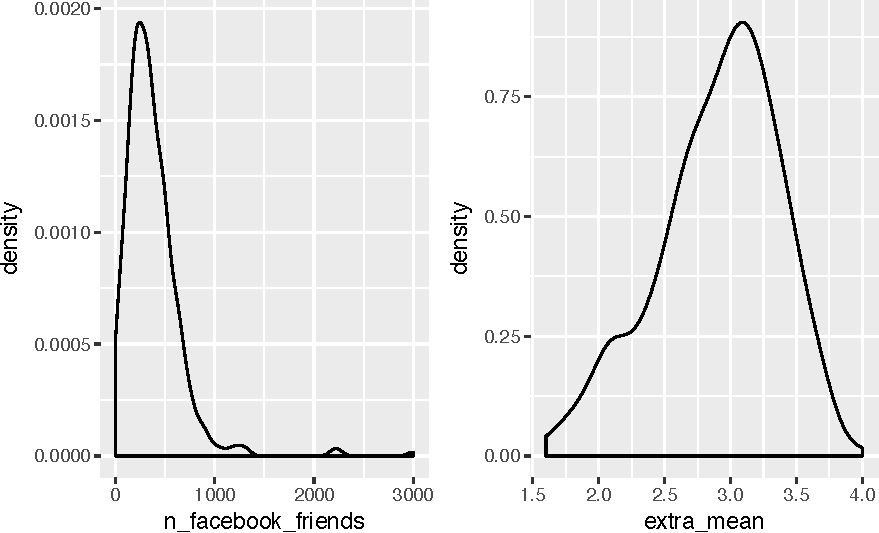
\includegraphics[width=0.7\linewidth]{043_Typische_Probleme_Datenanalyse_files/figure-latex/fig-norm-check-1} 

}

\caption{Visuelles Prüfen der Normalverteilung}\label{fig:fig-norm-check}
\end{figure}

Während die der mittlere Extraversionswert recht gut normalverteilt ist,
ist die Anzahl der Facebookfreunde ordentlich (rechts-)schief. Bei
schiefen Verteilung können Transformationen Abhilfe schaffen; ein Thema,
auf das wir hier nicht weiter eingehen.

\subsection{\texorpdfstring{Werte umkodieren und partionieren
(``binnen'')}{Werte umkodieren und partionieren (binnen)}}\label{werte-umkodieren-und-partionieren-binnen}

\emph{Umkodieren}\index{Umkodieren} meint, die Werte zu ändern. Man
sieht immer mal wieder, dass die Variable ``gender'' (Geschlecht) mit
\texttt{1} und \texttt{2} kodiert ist. Verwechslungen sind da
vorprogrammiert (``Ich bin mir echt ziemlich sicher, dass ich 1 für
Männer kodiert habe, wahrscheinlich\ldots{}''). Besser wäre es, die
Ausprägungen \texttt{male} und \texttt{female} (``Mann'', ``Frau'') o.ä.
zu verwenden (vgl. Abb. \ref{fig:umkodieren}).

\begin{figure}

{\centering 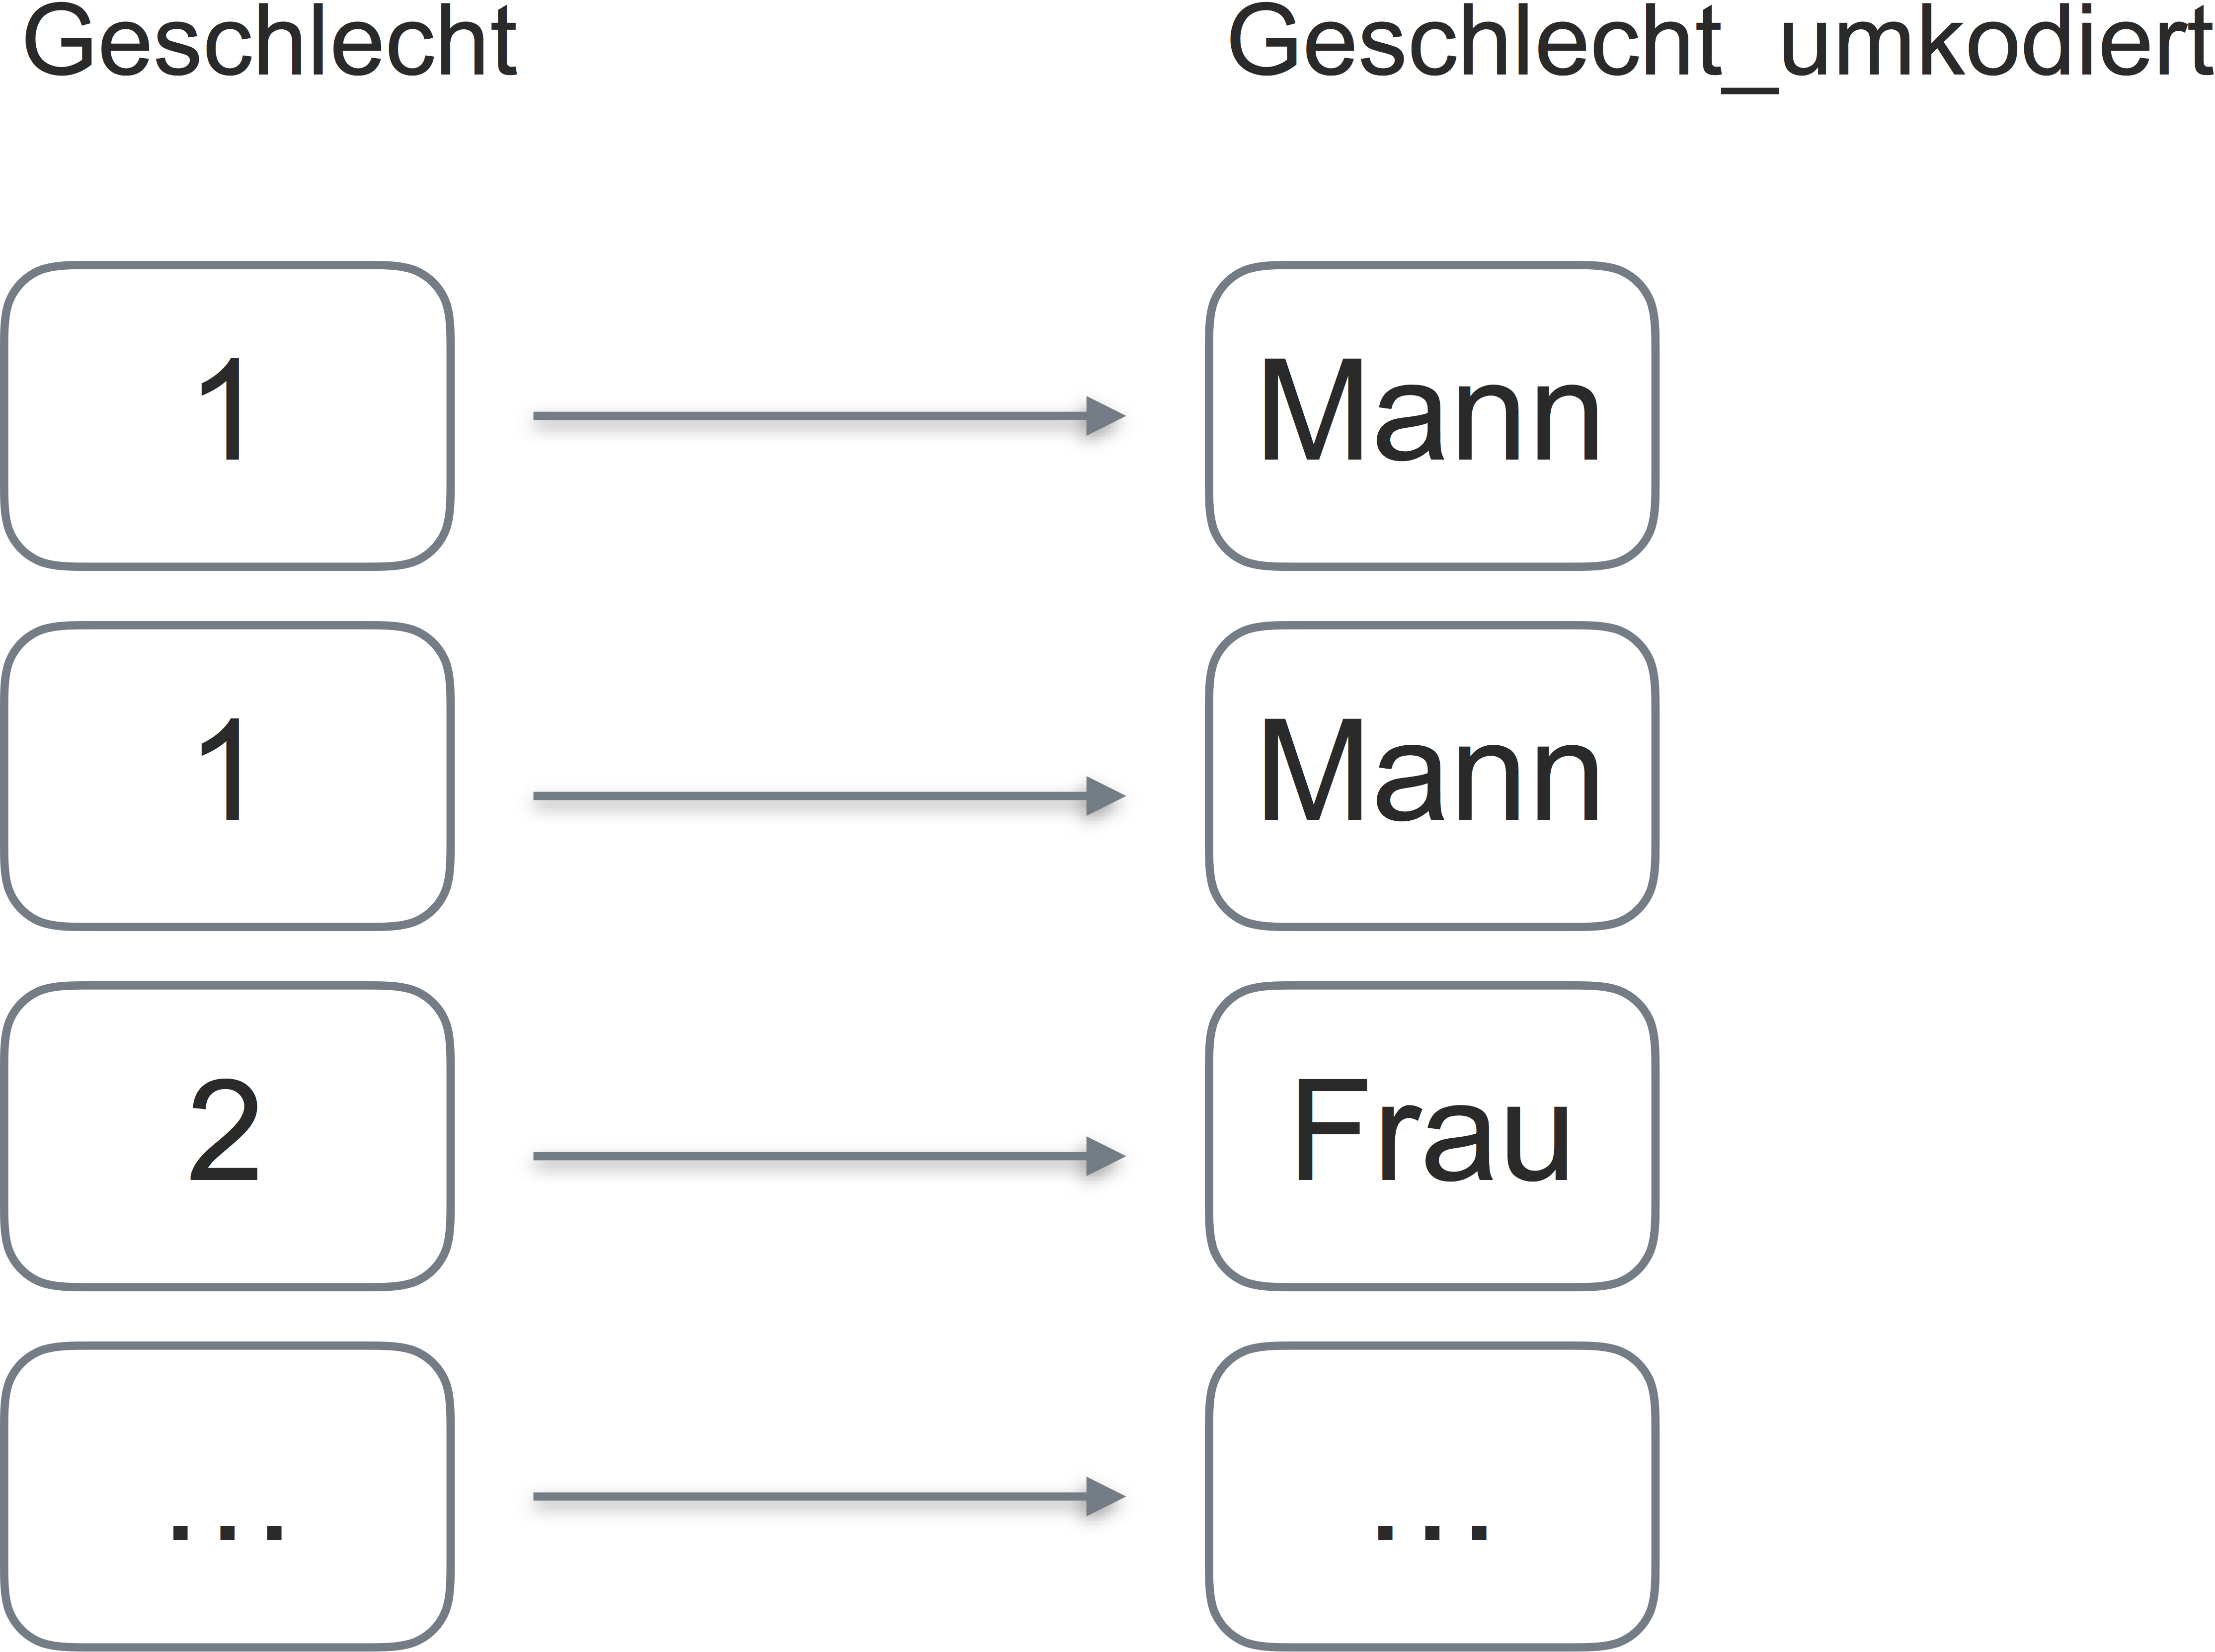
\includegraphics[width=0.7\linewidth]{images/typ_prob/umkodieren_crop} 

}

\caption{Sinnbild für Umkodieren}\label{fig:umkodieren}
\end{figure}

Partionieren\index\{Partionieren) oder \emph{``Binnen''}\index{Binnen}
meint, eine kontinuierliche Variablen in einige Bereiche (mindestens 2)
zu zerschneiden. Damit macht man aus einer kontinuierlichen Variablen
eine diskrete. Ein Bild erläutert das am einfachsten (vgl. Abb.
\ref{fig:cut-schere}).

\begin{figure}

{\centering 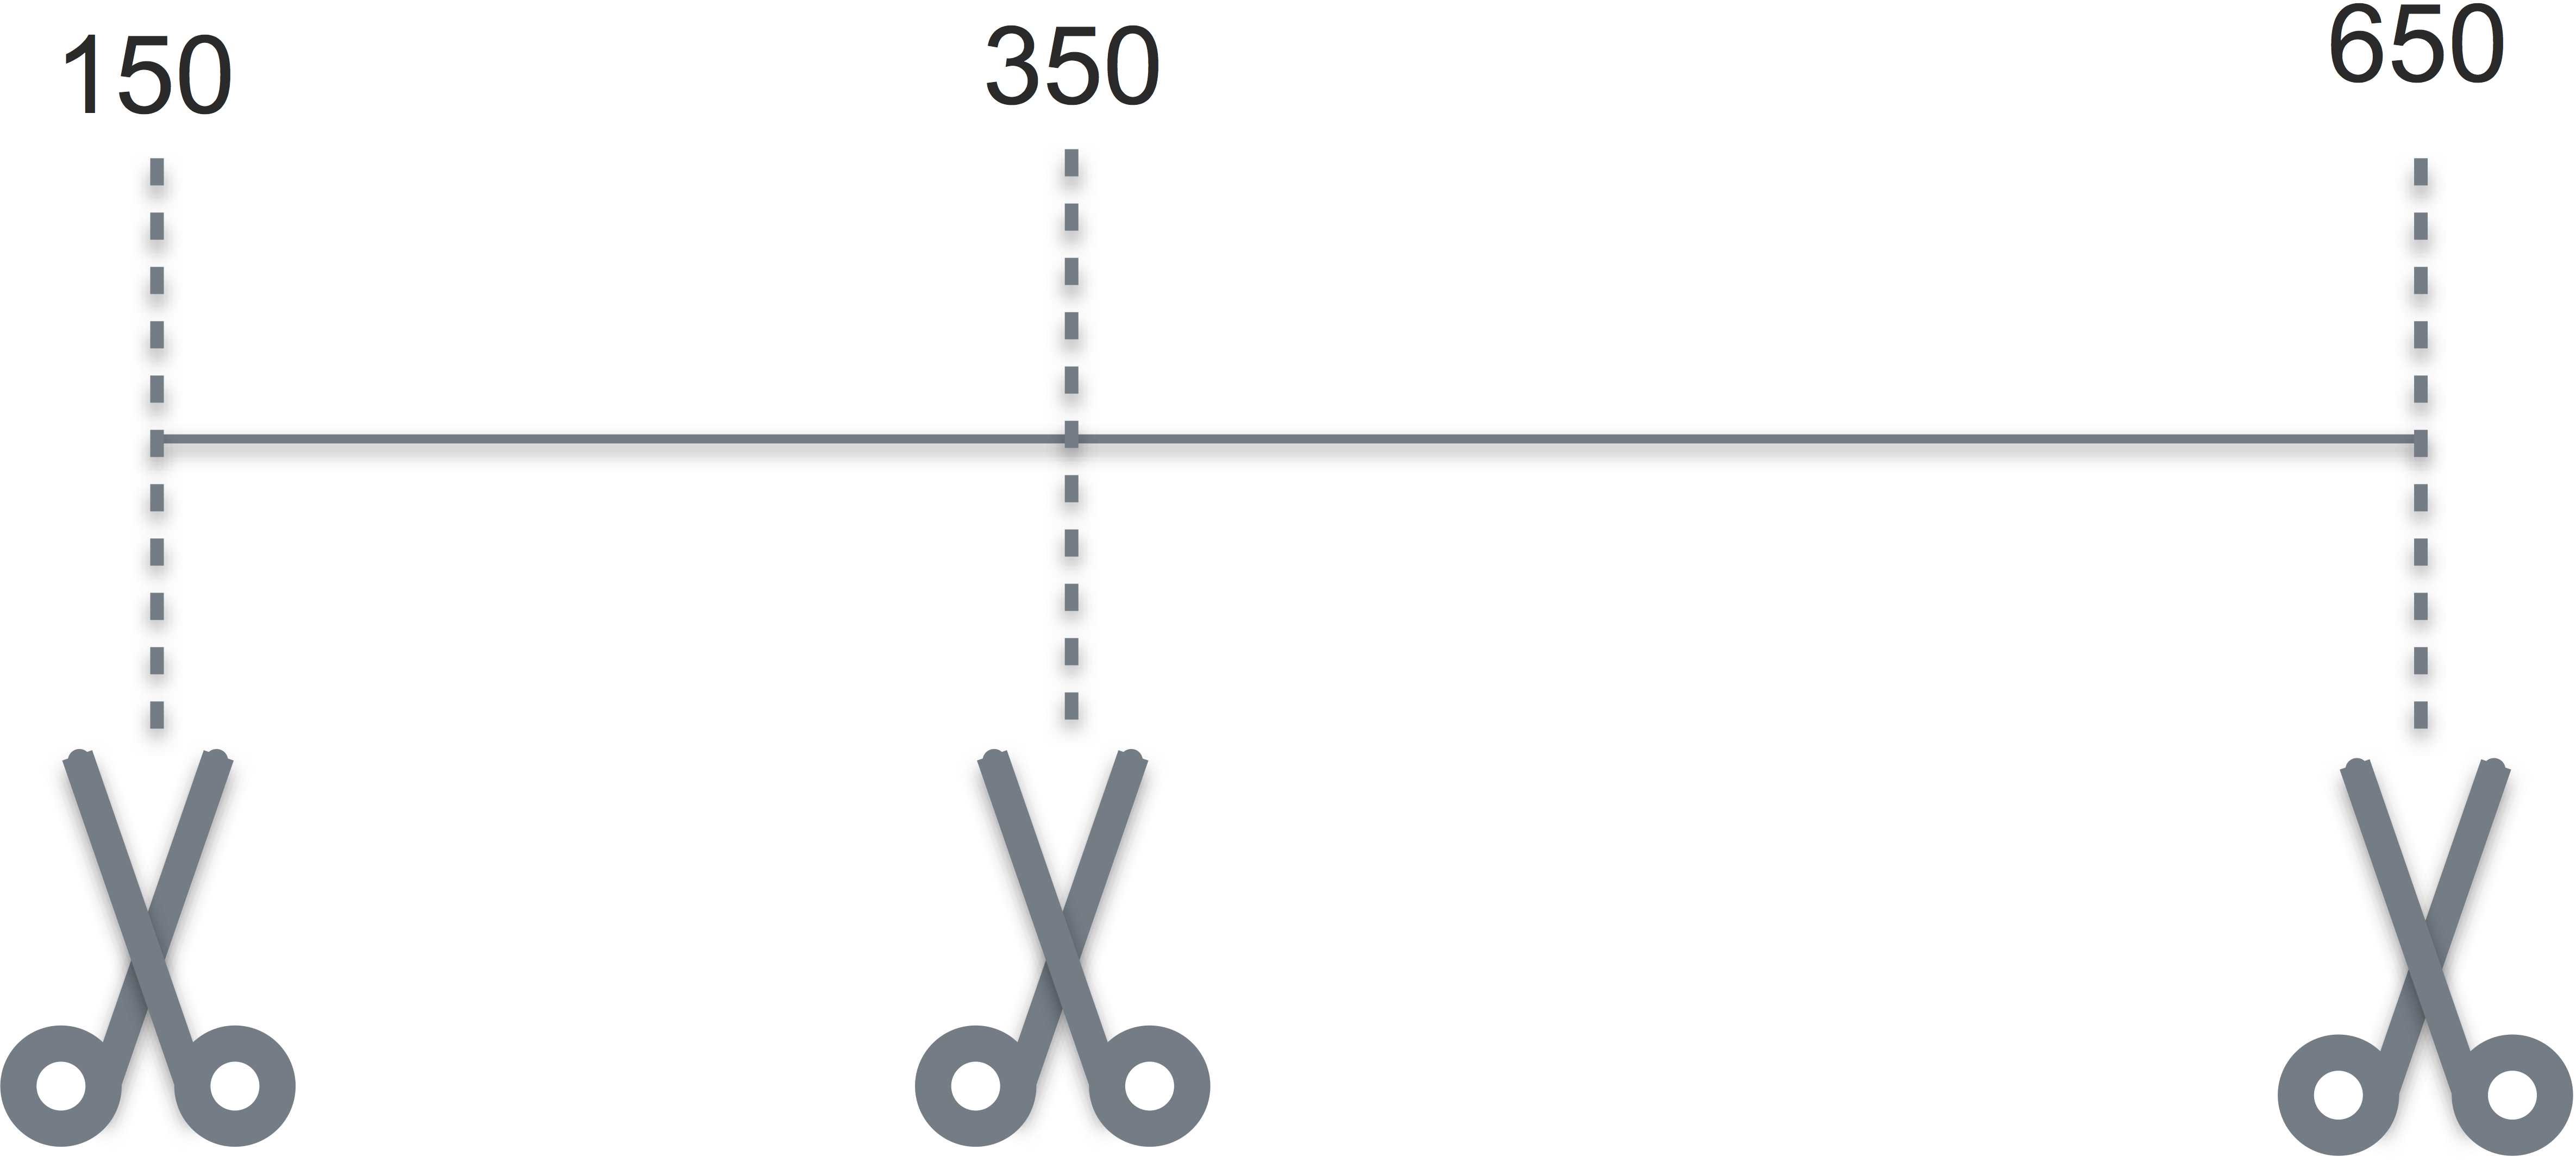
\includegraphics[width=0.7\linewidth]{images/typ_prob/cut_schere_crop} 

}

\caption{Sinnbild zum 'Binnen'}\label{fig:cut-schere}
\end{figure}

\subsubsection{\texorpdfstring{Umkodieren und partionieren mit
\texttt{car::recode}}{Umkodieren und partionieren mit car::recode}}\label{umkodieren-und-partionieren-mit-carrecode}

Manchmal möchte man z.B. negativ gepolte Items umdrehen oder bei
kategoriellen Variablen kryptische Bezeichnungen in sprechendere
umwandeln. Hier gibt es eine Reihe praktischer Befehle, z.B.
\texttt{recode} aus dem Paket \texttt{car}. Schauen wir uns ein paar
Beispiele zum Umkodieren an.

\begin{Shaded}
\begin{Highlighting}[]

\NormalTok{stats_test <-}\StringTok{ }\KeywordTok{read.csv}\NormalTok{(}\StringTok{"data/test_inf_short.csv"}\NormalTok{)}

\NormalTok{stats_test$score_fac <-}\StringTok{ }\NormalTok{car::}\KeywordTok{recode}\NormalTok{(stats_test$study_time, }
                        \StringTok{"5 = 'sehr viel'; 2:4 = 'mittel'; 1 = 'wenig'"}\NormalTok{,}
                        \DataTypeTok{as.factor.result =} \OtherTok{TRUE}\NormalTok{)}
\NormalTok{stats_test$score_fac <-}\StringTok{ }\NormalTok{car::}\KeywordTok{recode}\NormalTok{(stats_test$study_time, }
                        \StringTok{"5 = 'sehr viel'; 2:4 = 'mittel'; 1 = 'wenig'"}\NormalTok{,}
                        \DataTypeTok{as.factor.result =} \OtherTok{FALSE}\NormalTok{)}

\NormalTok{stats_test$study_time_2 <-}\StringTok{ }\NormalTok{car::}\KeywordTok{recode}\NormalTok{(stats_test$study_time, }
                                       \StringTok{"5 = 'sehr viel'; 4 = 'wenig'; }
\StringTok{                                       else = 'Hilfe'"}\NormalTok{, }
                                       \DataTypeTok{as.factor.result =} \OtherTok{TRUE}\NormalTok{)}

\KeywordTok{head}\NormalTok{(stats_test$study_time_2)}
\CommentTok{#> [1] sehr viel Hilfe     sehr viel Hilfe     wenig     Hilfe    }
\CommentTok{#> Levels: Hilfe sehr viel wenig}
\end{Highlighting}
\end{Shaded}

Der Befehle \texttt{recode} ist praktisch; mit \texttt{:} kann man ``von
bis'' ansprechen (das ginge mit \texttt{c()} übrigens auch);
\texttt{else} für ``ansonsten'' ist möglich und mit
\texttt{as.factor.result} kann man entweder einen Faktor oder eine
Text-Variable zurückgeliefert bekommen. Der ganze ``Wechselterm'' steht
in Anführungsstrichen (\texttt{"}). Einzelne Teile des Wechselterms sind
mit einem Strichpunkt (\texttt{;}) voneinander getrennt.

Das klassische Umkodieren von Items aus Fragebögen kann man so
anstellen; sagen wir \texttt{interest} soll umkodiert werden:

\begin{Shaded}
\begin{Highlighting}[]
\NormalTok{stats_test$no_interest <-}\StringTok{ }\NormalTok{car::}\KeywordTok{recode}\NormalTok{(stats_test$interest, }
                                      \StringTok{"1 = 6; 2 = 5; 3 = 4; 4 = 3; }
\StringTok{                                      5 = 2; 6 = 1; else = NA"}\NormalTok{)}
\KeywordTok{glimpse}\NormalTok{(stats_test$no_interest)}
\CommentTok{#>  num [1:306] 2 4 1 5 1 NA NA 4 2 2 ...}
\end{Highlighting}
\end{Shaded}

Bei dem Wechselterm muss man aufpassen, nichts zu verwechseln; die
Zahlen sehen alle ähnlich aus\ldots{}

Testen kann man den Erfolg des Umpolens mit

\begin{Shaded}
\begin{Highlighting}[]
\NormalTok{dplyr::}\KeywordTok{count}\NormalTok{(stats_test, interest)}
\CommentTok{#> # A tibble: 7 x 2}
\CommentTok{#>   interest     n}
\CommentTok{#>      <int> <int>}
\CommentTok{#> 1        1    30}
\CommentTok{#> 2        2    47}
\CommentTok{#> 3        3    66}
\CommentTok{#> 4        4    41}
\CommentTok{#> 5        5    45}
\CommentTok{#> 6        6     9}
\CommentTok{#> 7       NA    68}
\NormalTok{dplyr::}\KeywordTok{count}\NormalTok{(stats_test, no_interest)}
\CommentTok{#> # A tibble: 7 x 2}
\CommentTok{#>   no_interest     n}
\CommentTok{#>         <dbl> <int>}
\CommentTok{#> 1           1     9}
\CommentTok{#> 2           2    45}
\CommentTok{#> 3           3    41}
\CommentTok{#> 4           4    66}
\CommentTok{#> 5           5    47}
\CommentTok{#> 6           6    30}
\CommentTok{#> 7          NA    68}
\end{Highlighting}
\end{Shaded}

Scheint zu passen. Noch praktischer ist, dass man so auch numerische
Variablen in Bereiche aufteilen kann (``binnen''):

\begin{Shaded}
\begin{Highlighting}[]
\NormalTok{stats_test$Ergebnis <-}\StringTok{ }\NormalTok{car::}\KeywordTok{recode}\NormalTok{(stats_test$score, }
                                   \StringTok{"1:38 = 'durchgefallen'; }
\StringTok{                                   else = 'bestanden'"}\NormalTok{)}
\end{Highlighting}
\end{Shaded}

Natürlich gibt es auch eine Pfeifen kompatible Version, um Variablen
umzukodieren bzw. zu binnen: \texttt{dplyr::recode}\footnote{\url{https://blog.rstudio.org/2016/06/27/dplyr-0-5-0/}}.
Die Syntax ist allerdings etwas weniger komfortabel (da strenger), so
dass wir an dieser Stelle bei \texttt{car::recode} bleiben.

\subsubsection{Einfaches Umkodieren mit einer
Logik-Prüfung}\label{einfaches-umkodieren-mit-einer-logik-prufung}

Nehmen wir an, wir möchten die Anzahl der Punkte in einer
Statistikklausur (\texttt{score}) umkodieren in eine Variable
``bestanden'' mit den zwei Ausprägungen ``ja'' und ``nein''; der
griesgrämige Professor beschließt, dass die Klausur ab 25 Punkten (von
40) bestanden sei. Die Umkodierung ist also von der Art ``viele
Ausprägungen in zwei Ausprägungen umkodieren''. Das kann man z.B. so
erledigen:

\begin{Shaded}
\begin{Highlighting}[]
\NormalTok{stats_test$bestanden <-}\StringTok{ }\NormalTok{stats_test$score >}\StringTok{ }\DecValTok{24}

\KeywordTok{head}\NormalTok{(stats_test$bestanden)}
\CommentTok{#> [1]  TRUE  TRUE  TRUE FALSE  TRUE  TRUE}
\end{Highlighting}
\end{Shaded}

Genauso könnte man sich die ``Grenzfälle'' - die Bemitleidenswerten mit
24 Punkten - anschauen (knapp daneben ist auch vorbei, so der
griesgrämige Professor weiter):

\begin{Shaded}
\begin{Highlighting}[]
\NormalTok{stats_test$Grenzfall <-}\StringTok{ }\NormalTok{stats_test$score ==}\StringTok{ }\DecValTok{24}

\KeywordTok{count}\NormalTok{(stats_test, Grenzfall)}
\CommentTok{#> # A tibble: 2 x 2}
\CommentTok{#>   Grenzfall     n}
\CommentTok{#>       <lgl> <int>}
\CommentTok{#> 1     FALSE   294}
\CommentTok{#> 2      TRUE    12}
\end{Highlighting}
\end{Shaded}

Natürlich könnte man auch hier ``Durchpfeifen'':

\begin{Shaded}
\begin{Highlighting}[]
\NormalTok{stats_test <-}\StringTok{ }
\NormalTok{stats_test %>%}\StringTok{ }
\StringTok{  }\KeywordTok{mutate}\NormalTok{(}\DataTypeTok{Grenzfall =} \NormalTok{score ==}\StringTok{ }\DecValTok{24}\NormalTok{)}

\KeywordTok{count}\NormalTok{(stats_test, Grenzfall)}
\CommentTok{#> # A tibble: 2 x 2}
\CommentTok{#>   Grenzfall     n}
\CommentTok{#>       <lgl> <int>}
\CommentTok{#> 1     FALSE   294}
\CommentTok{#> 2      TRUE    12}
\end{Highlighting}
\end{Shaded}

\subsubsection{\texorpdfstring{Binnen mit
\texttt{cut}}{Binnen mit cut}}\label{binnen-mit-cut}

Numerische Werte in Klassen zu gruppieren (``to bin'', denglisch:
``binnen'') kann mit dem Befehl \texttt{cut} (and friends) besorgt
werden.

Es lassen sich drei typische Anwendungsformen unterscheiden:

Eine numerische Variable \ldots{}

\begin{enumerate}
\def\labelenumi{\arabic{enumi}.}
\tightlist
\item
  in \emph{k} gleich große Klassen gruppieren (gleichgroße Intervalle)
\item
  so in Klassen gruppieren, dass in jeder Klasse \emph{n} Beobachtungen
  sind (gleiche Gruppengrößen)
\item
  in beliebige Klassen gruppieren
\end{enumerate}

\paragraph{Gleichgroße Intervalle}\label{gleichgroe-intervalle}

Nehmen wir an, wir möchten die numerische Variable ``Körpergröße'' in
drei Gruppen einteilen: ``klein'', ``mittel'' und ``groß''. Der Range
von Körpergröße soll gleichmäßig auf die drei Gruppen aufgeteilt werden,
d.h. der Range (Intervall) der drei Gruppen soll gleich groß sein. Dazu
kann man \texttt{cut\_interval} aus \texttt{ggplot2} nehmen\footnote{d.h.
  \texttt{ggplot2} muss geladen sein; wenn man \texttt{tidyverse} lädt,
  wird \texttt{ggplot2} automatisch auch geladen}.

\begin{Shaded}
\begin{Highlighting}[]
\NormalTok{stats_test <-}\StringTok{ }\KeywordTok{read.csv}\NormalTok{(}\StringTok{"data/test_inf_short.csv"}\NormalTok{)}


\NormalTok{temp <-}\StringTok{ }\KeywordTok{cut_interval}\NormalTok{(}\DataTypeTok{x =} \NormalTok{stats_test$score, }\DataTypeTok{n =} \DecValTok{3}\NormalTok{)}

\KeywordTok{levels}\NormalTok{(temp)}
\CommentTok{#> [1] "[17,24.7]"   "(24.7,32.3]" "(32.3,40]"}
\end{Highlighting}
\end{Shaded}

\texttt{cut\_interval} liefert eine Variable vom Typ \texttt{factor}
zurück. Hier haben wir das Punktespektrum in drei gleich große Bereiche
unterteilt (d.h. mit jeweils gleichem Punkte-Range).

\paragraph{Gleiche Gruppengrößen}\label{gleiche-gruppengroen}

\begin{Shaded}
\begin{Highlighting}[]
\NormalTok{temp <-}\StringTok{ }\KeywordTok{cut_number}\NormalTok{(stats_test$score, }\DataTypeTok{n =} \DecValTok{2}\NormalTok{)}
\KeywordTok{str}\NormalTok{(temp)}
\CommentTok{#>  Factor w/ 2 levels "[17,31]","(31,40]": 1 1 2 1 2 2 2 1 1 2 ...}
\KeywordTok{median}\NormalTok{(stats_test$score)}
\CommentTok{#> [1] 31}
\end{Highlighting}
\end{Shaded}

Mit \texttt{cut\_number} (aus ggplot2) kann man einen Vektor in
\texttt{n} Gruppen mit (etwa) gleich viel Observationen einteilen. Hier
haben wir \texttt{score} am Median geteilt.

\begin{quote}
Teilt man einen Vektor in zwei gleich große Gruppen, so entspricht das
einer Aufteilung am Median (Median-Split).
\end{quote}

\paragraph{In beliebige Klassen
gruppieren}\label{in-beliebige-klassen-gruppieren}

\begin{Shaded}
\begin{Highlighting}[]
\NormalTok{stats_test$punkte_gruppe <-}\StringTok{ }\KeywordTok{cut}\NormalTok{(stats_test$score, }
                             \DataTypeTok{breaks =} \KeywordTok{c}\NormalTok{(-}\OtherTok{Inf}\NormalTok{, }\DecValTok{25}\NormalTok{, }\DecValTok{29}\NormalTok{, }\DecValTok{33}\NormalTok{, }\DecValTok{37}\NormalTok{, }\DecValTok{40}\NormalTok{),}
                             \DataTypeTok{labels =} \KeywordTok{c}\NormalTok{(}\StringTok{"5"}\NormalTok{, }\StringTok{"4"}\NormalTok{, }\StringTok{"3"}\NormalTok{, }\StringTok{"2"}\NormalTok{, }\StringTok{"1"}\NormalTok{))}

\KeywordTok{count}\NormalTok{(stats_test, punkte_gruppe)}
\CommentTok{#> # A tibble: 5 x 2}
\CommentTok{#>   punkte_gruppe     n}
\CommentTok{#>          <fctr> <int>}
\CommentTok{#> 1             5    56}
\CommentTok{#> 2             4    68}
\CommentTok{#> 3             3    63}
\CommentTok{#> 4             2    64}
\CommentTok{#> 5             1    55}
\end{Highlighting}
\end{Shaded}

\texttt{cut} ist im Standard-R (Paket ``base'') enthalten. Mit
\texttt{breaks} gibt man die Intervallgrenzen an. Zu beachten ist, dass
man eine Unter- bzw. Obergrenze angeben muss. D.h. der kleinste Wert in
der Stichprobe wird nicht automatisch als unterste Intervallgrenze
herangezogen. Anschaulich gesprochen ist \texttt{cut} ein Messer, das
ein Seil (die kontinuierliche Variable) mit einem oder mehreren
Schnitten zerschneidet (vgl. Abb. \ref{fig:cut-schere}). Wenn wir 6
Schnitte (\texttt{breaks}) tun, haben wir 5 Teile, wie Abb.
\ref{fig:cut-schere} zeigt. Darum müssen wir auch nur 5 (6-1)
\texttt{labels} für die Teile vergeben.

\section{Deskriptive Statistiken
berechnen}\label{deskriptive-statistiken-berechnen}

\subsection{Mittelwerte pro Zeile
berechnen}\label{mittelwerte-pro-zeile-berechnen}

\subsubsection{\texorpdfstring{\texttt{rowMeans}}{rowMeans}}\label{rowmeans}

Um Umfragedaten auszuwerten, will man häufig einen Mittelwert \emph{pro
Zeile} berechnen. Normalerweise fasst man eine \emph{Spalte} zu einer
Zahl zusammen; aber jetzt, fassen wir eine \emph{Zeile} zu einer Zahl
zusammen. Der häufigste Fall ist, wie gesagt, einen Mittelwert zu bilden
für jede Person. Nehmen wir an, wir haben eine Befragung zur
Extraversion durchgeführt und möchten jetzt den mittleren
Extraversions-Wert pro Person (d.h. pro Zeile) berechnen.

\begin{Shaded}
\begin{Highlighting}[]
\NormalTok{extra <-}\StringTok{ }\KeywordTok{read.csv}\NormalTok{(}\StringTok{"data/extra.csv"}\NormalTok{)}

\NormalTok{extra_items <-}\StringTok{ }\NormalTok{extra %>%}\StringTok{ }
\StringTok{  }\KeywordTok{select}\NormalTok{(i01:i10)  }\CommentTok{# `select` ist aus `dplyr`}

\CommentTok{# oder:}
\CommentTok{# select(extra_items, i01:i10)}

\NormalTok{extra$extra_mw <-}\StringTok{ }\KeywordTok{rowMeans}\NormalTok{(extra_items)}
\end{Highlighting}
\end{Shaded}

Da der Datensatz über 28 Spalten verfügt, wir aber nur 10 Spalten
heranziehen möchten, um Zeilen auf eine Zahl zusammenzufassen, bilden
wir als Zwischenschritt einen ``schmäleren'' Datensatz,
\texttt{extra\_items}. Im Anschluss berechnen wir mit \texttt{rowMeans}
die Mittelwerte pro Zeile (engl. ``row'').

\subsection{Mittelwerte pro Spalte
berechnen}\label{mittelwerte-pro-spalte-berechnen}

Eine Möglichkeit ist der Befehl \texttt{summary} aus \texttt{dplyr}.

\begin{Shaded}
\begin{Highlighting}[]
\NormalTok{stats_test %>%}\StringTok{ }
\StringTok{  }\NormalTok{na.omit %>%}\StringTok{ }
\StringTok{  }\KeywordTok{summarise}\NormalTok{(}\KeywordTok{mean}\NormalTok{(score),}
            \KeywordTok{sd}\NormalTok{(score),}
            \KeywordTok{median}\NormalTok{(score),}
            \KeywordTok{IQR}\NormalTok{(score))}
\CommentTok{#>   mean(score) sd(score) median(score) IQR(score)}
\CommentTok{#> 1        30.6      5.72            31          9}
\end{Highlighting}
\end{Shaded}

Die Logik von \texttt{dplyr} lässt auch einfach Subgruppenanalysen zu.
Z.B. können wir eine Teilmenge des Datensatzes mit \texttt{filter}
erstellen und dann mit \texttt{group\_by} Gruppen vergleichen:

\begin{Shaded}
\begin{Highlighting}[]
\NormalTok{stats_test %>%}\StringTok{ }
\StringTok{  }\KeywordTok{filter}\NormalTok{(study_time >}\StringTok{ }\DecValTok{1}\NormalTok{) %>%}\StringTok{ }
\StringTok{  }\KeywordTok{group_by}\NormalTok{(interest) %>%}\StringTok{ }
\StringTok{  }\KeywordTok{summarise}\NormalTok{(}\KeywordTok{median}\NormalTok{(score, }\DataTypeTok{na.rm =} \OtherTok{TRUE}\NormalTok{))}
\CommentTok{#> # A tibble: 6 x 2}
\CommentTok{#>   interest `median(score, na.rm = TRUE)`}
\CommentTok{#>      <int>                         <dbl>}
\CommentTok{#> 1        1                            28}
\CommentTok{#> 2        2                            30}
\CommentTok{#> 3        3                            33}
\CommentTok{#> 4        4                            31}
\CommentTok{#> 5        5                            34}
\CommentTok{#> 6        6                            34}
\end{Highlighting}
\end{Shaded}

Wir können auch Gruppierungskriterien unterwegs erstellen:

\begin{Shaded}
\begin{Highlighting}[]
\NormalTok{stats_test %>%}\StringTok{ }
\StringTok{  }\NormalTok{na.omit %>%}\StringTok{ }
\StringTok{  }\KeywordTok{filter}\NormalTok{(study_time >}\StringTok{ }\DecValTok{1}\NormalTok{) %>%}\StringTok{ }
\StringTok{  }\KeywordTok{group_by}\NormalTok{(}\DataTypeTok{intessiert =} \NormalTok{interest >}\StringTok{ }\DecValTok{3}\NormalTok{) %>%}\StringTok{ }
\StringTok{  }\KeywordTok{summarise}\NormalTok{(}\KeywordTok{median}\NormalTok{(score))}
\CommentTok{#> # A tibble: 2 x 2}
\CommentTok{#>   intessiert `median(score)`}
\CommentTok{#>        <lgl>           <dbl>}
\CommentTok{#> 1      FALSE              30}
\CommentTok{#> 2       TRUE              32}
\end{Highlighting}
\end{Shaded}

Die beiden Gruppen von \texttt{interessiert} sind ``ja, interessiert''
(\texttt{interest\ \textgreater{}\ 3} ist \texttt{TRUE}) und ``nein,
nicht interessiert'' (\texttt{interest\ \textgreater{}\ 3} ist
\texttt{FALSE}).

Etwas expliziter wäre es, \texttt{mutate} zu verwenden, um die Variable
\texttt{interessiert} zu erstellen:

\begin{Shaded}
\begin{Highlighting}[]
\NormalTok{stats_test %>%}\StringTok{ }
\StringTok{  }\NormalTok{na.omit %>%}\StringTok{ }
\StringTok{  }\KeywordTok{filter}\NormalTok{(study_time >}\StringTok{ }\DecValTok{1}\NormalTok{) %>%}\StringTok{ }
\StringTok{  }\KeywordTok{mutate}\NormalTok{(}\DataTypeTok{interessiert =} \NormalTok{interest >}\StringTok{ }\DecValTok{3}\NormalTok{) %>%}\StringTok{ }
\StringTok{  }\KeywordTok{group_by}\NormalTok{(interessiert) %>%}\StringTok{ }
\StringTok{  }\KeywordTok{summarise}\NormalTok{(}\KeywordTok{median}\NormalTok{(score))}
\CommentTok{#> # A tibble: 2 x 2}
\CommentTok{#>   interessiert `median(score)`}
\CommentTok{#>          <lgl>           <dbl>}
\CommentTok{#> 1        FALSE              30}
\CommentTok{#> 2         TRUE              32}
\end{Highlighting}
\end{Shaded}

\BeginKnitrBlock{rmdcaution}
Statistiken, die auf dem Mittelwert (arithmetisches Mittel) beruhen,
sind nicht robust gegenüber Ausreißer: Schon wenige Extremwerte können
diese Statistiken so verzerren, dass sie erheblich an Aussagekraft
verlieren.

Daher: besser robuste Statistiken verwenden. Der Median, der Modus und
der IQR bieten sich an.
\EndKnitrBlock{rmdcaution}

\subsection{Korrelationstabellen
berechnen}\label{korrelationstabellen-berechnen}

Korrelationen bzw. Korrelationstabellen lassen sich mit dem
R-Standardbefehl \texttt{cor} berechnen:

\begin{Shaded}
\begin{Highlighting}[]

\NormalTok{stats_test %>%}\StringTok{ }
\StringTok{  }\KeywordTok{select}\NormalTok{(study_time,interest,score) %>%}\StringTok{ }
\StringTok{  }\KeywordTok{cor}\NormalTok{()}
\CommentTok{#>            study_time interest score}
\CommentTok{#> study_time          1       NA    NA}
\CommentTok{#> interest           NA        1    NA}
\CommentTok{#> score              NA       NA     1}
\end{Highlighting}
\end{Shaded}

Oh! Lauter NAs! Besser wir löschen Zeilen mit fehlenden Werten bevor wir
die Korrelation ausrechnen:

\begin{Shaded}
\begin{Highlighting}[]
\NormalTok{stats_test %>%}\StringTok{ }
\StringTok{  }\KeywordTok{select}\NormalTok{(study_time:score) %>%}\StringTok{ }
\StringTok{  }\NormalTok{na.omit %>%}\StringTok{ }
\StringTok{  }\KeywordTok{cor}\NormalTok{()}
\CommentTok{#>            study_time self_eval interest score}
\CommentTok{#> study_time      1.000     0.559    0.461 0.441}
\CommentTok{#> self_eval       0.559     1.000    0.360 0.628}
\CommentTok{#> interest        0.461     0.360    1.000 0.223}
\CommentTok{#> score           0.441     0.628    0.223 1.000}
\end{Highlighting}
\end{Shaded}

Alternativ zu \texttt{cor} kann man auch \texttt{corrr:correlate}
verwenden:

\begin{Shaded}
\begin{Highlighting}[]

\NormalTok{stats_test %>%}\StringTok{ }
\StringTok{  }\KeywordTok{select}\NormalTok{(study_time:score) %>%}\StringTok{ }
\StringTok{  }\NormalTok{correlate}
\CommentTok{#> # A tibble: 4 x 5}
\CommentTok{#>      rowname study_time self_eval interest score}
\CommentTok{#>        <chr>      <dbl>     <dbl>    <dbl> <dbl>}
\CommentTok{#> 1 study_time         NA     0.559    0.461 0.441}
\CommentTok{#> 2  self_eval      0.559        NA    0.360 0.628}
\CommentTok{#> 3   interest      0.461     0.360       NA 0.223}
\CommentTok{#> 4      score      0.441     0.628    0.223    NA}
\end{Highlighting}
\end{Shaded}

\texttt{correlate} hat den Vorteil, dass es bei fehlenden Werten einen
Wert ausgibt; die Korrelation wird paarweise mit den verfügbaren
(nicht-fehlenden) Werten berechnet. Außerdem wird eine Dataframe
(genauer: tibble) zurückgeliefert, was häufig praktischer ist zur
Weiterverarbeitung. Wir könnten jetzt die resultierende
Korrelationstabelle plotten, vorher ``rasieren'' wir noch das
redundanten obere Dreieck ab (da Korrelationstabellen ja symmetrisch
sind):

\begin{Shaded}
\begin{Highlighting}[]
\NormalTok{stats_test %>%}\StringTok{ }
\StringTok{  }\KeywordTok{select}\NormalTok{(study_time:score) %>%}\StringTok{ }
\StringTok{  }\NormalTok{correlate %>%}\StringTok{ }
\StringTok{  }\NormalTok{shave %>%}\StringTok{ }
\StringTok{  }\NormalTok{rplot}
\end{Highlighting}
\end{Shaded}

\begin{center}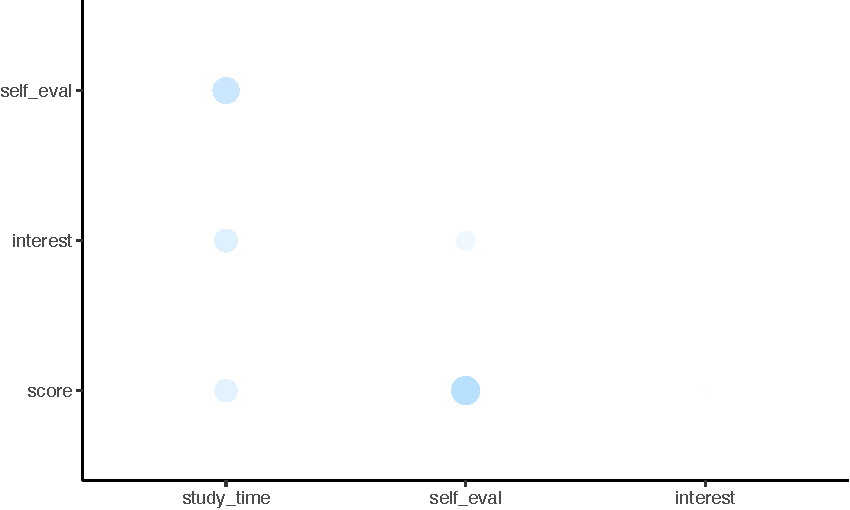
\includegraphics[width=0.7\linewidth]{043_Typische_Probleme_Datenanalyse_files/figure-latex/rplot-demo-1} \end{center}

\section{Befehlsübersicht}\label{befehlsubersicht-3}

Tabelle \ref{tab:befehle-praxisprobleme} stellt die Befehle dieses
Kapitels dar.

\begin{table}

\caption{\label{tab:befehle-praxisprobleme}Befehle des Kapitels 'Praxisprobleme'}
\centering
\begin{tabular}[t]{l|l}
\hline
Paket::Funktion & Beschreibung\\
\hline
na.omit & Löscht Zeilen, die fehlende Werte enthalten\\
\hline
nrow & Liefert die Anzahl der Zeilen des Dataframes zurück\\
\hline
complete.cases & Gibt die Zeilen ohne fehlenden Werte eines Dataframes zurück\\
\hline
car::recode & Kodiert Werte um\\
\hline
cut & Schneidet eine kontinuierliche Variable in Wertebereiche\\
\hline
rowMeans & Berechnet Zeilen-Mittelwerte\\
\hline
dplyr::rowwise & Gruppiert nach Zeilen\\
\hline
ggplot2::cut\_number & Schneidet eine kontinuierliche Variable in n gleich große Bereiche\\
\hline
ggplot2::cut\_interval & Schneidet eine kontinuierliche Variable in Intervalle der Größe k\\
\hline
head & Zeigt nur die ersten Zeilen/Werte eines Dataframes/Vektors an.\\
\hline
scale & z-skaliert eine Variable\\
\hline
dplyr::select\_if & Wählt eine Spalte aus, wenn ein Kriterium erfüllt ist\\
\hline
dplyr::glimpse & Gibt einen Überblick über einen Dataframe\\
\hline
dplyr::mutate\_if & definiert eine Spalte, wenn eine Kriterium erfüllt ist\\
\hline
: & Definiert einen Bereich von … bis …\\
\hline
corrr::correlate & Berechnet Korrelationtabelle, liefert einen Dataframe zurück\\
\hline
cor & Berechnet Korrelationtabelle\\
\hline
corrr::rplot & Plottet Korrelationsmatrix von correlate\\
\hline
corrr::shave & “Rasiert” redundantes Dreick in Korrelationsmatrix ab\\
\hline
\end{tabular}
\end{table}

\chapter{\texorpdfstring{Fallstudie
`movies'}{Fallstudie movies}}\label{case-movies}

\begin{center}
\includegraphics[width=0.3\linewidth]{images/FOM} \end{center}

\begin{center}
\includegraphics[width=0.1\linewidth]{images/licence} \end{center}

\BeginKnitrBlock{rmdcaution}
Lernziele:

\begin{itemize}
\tightlist
\item
  Grundlegende Funktionen von \texttt{dplyr} andwenden können.
\item
  Das Konzept der Pfeife in einem echten Datensatz anwenden können.
\item
  Auch mit relativ großen Daten sicher hantieren können.
\end{itemize}
\EndKnitrBlock{rmdcaution}

Der Datensatz \texttt{movies} enthält Bewertungen von Filmen, zusammen
mit einigen zusätzlichen Informationen wie Genre, Erscheinungsjahr und
Budgethöhe. Wir nutzen diesen Datensatz um uns einige Übung mit
Aufbereiten und Zusammenfassen von Daten zu verschaffen.

Für dieses Kapitel werden folgende Pakete benötigt:

\begin{Shaded}
\begin{Highlighting}[]
\KeywordTok{library}\NormalTok{(tidyverse)  }\CommentTok{# Datenjudo und Visualisierung}
\KeywordTok{library}\NormalTok{(corrr)}
\end{Highlighting}
\end{Shaded}

Zunächst laden wir die Daten und werfen einen Blick in den Datensatz:

\begin{Shaded}
\begin{Highlighting}[]
\NormalTok{movies <-}\StringTok{ }\KeywordTok{read.csv}\NormalTok{(}\StringTok{"data/movies.csv"}\NormalTok{)}
\KeywordTok{glimpse}\NormalTok{(movies)}
\CommentTok{#> Observations: 58,788}
\CommentTok{#> Variables: 24}
\CommentTok{#> $ title       <fctr> $, $1000 a Touchdown, $21 a Day Once a Month, $40...}
\CommentTok{#> $ year        <int> 1971, 1939, 1941, 1996, 1975, 2000, 2002, 2002, 19...}
\CommentTok{#> $ length      <int> 121, 71, 7, 70, 71, 91, 93, 25, 97, 61, 99, 96, 10...}
\CommentTok{#> $ budget      <int> NA, NA, NA, NA, NA, NA, NA, NA, NA, NA, NA, NA, NA...}
\CommentTok{#> $ rating      <dbl> 6.4, 6.0, 8.2, 8.2, 3.4, 4.3, 5.3, 6.7, 6.6, 6.0, ...}
\CommentTok{#> $ votes       <int> 348, 20, 5, 6, 17, 45, 200, 24, 18, 51, 23, 53, 44...}
\CommentTok{#> $ r1          <dbl> 4.5, 0.0, 0.0, 14.5, 24.5, 4.5, 4.5, 4.5, 4.5, 4.5...}
\CommentTok{#> $ r2          <dbl> 4.5, 14.5, 0.0, 0.0, 4.5, 4.5, 0.0, 4.5, 4.5, 0.0,...}
\CommentTok{#> $ r3          <dbl> 4.5, 4.5, 0.0, 0.0, 0.0, 4.5, 4.5, 4.5, 4.5, 4.5, ...}
\CommentTok{#> $ r4          <dbl> 4.5, 24.5, 0.0, 0.0, 14.5, 14.5, 4.5, 4.5, 0.0, 4....}
\CommentTok{#> $ r5          <dbl> 14.5, 14.5, 0.0, 0.0, 14.5, 14.5, 24.5, 4.5, 0.0, ...}
\CommentTok{#> $ r6          <dbl> 24.5, 14.5, 24.5, 0.0, 4.5, 14.5, 24.5, 14.5, 0.0,...}
\CommentTok{#> $ r7          <dbl> 24.5, 14.5, 0.0, 0.0, 0.0, 4.5, 14.5, 14.5, 34.5, ...}
\CommentTok{#> $ r8          <dbl> 14.5, 4.5, 44.5, 0.0, 0.0, 4.5, 4.5, 14.5, 14.5, 4...}
\CommentTok{#> $ r9          <dbl> 4.5, 4.5, 24.5, 34.5, 0.0, 14.5, 4.5, 4.5, 4.5, 4....}
\CommentTok{#> $ r10         <dbl> 4.5, 14.5, 24.5, 45.5, 24.5, 14.5, 14.5, 14.5, 24....}
\CommentTok{#> $ mpaa        <fctr> , , , , , , R, , , , , , , , PG-13, PG-13, , , , ...}
\CommentTok{#> $ Action      <int> 0, 0, 0, 0, 0, 0, 1, 0, 0, 0, 0, 0, 0, 0, 1, 1, 0,...}
\CommentTok{#> $ Animation   <int> 0, 0, 1, 0, 0, 0, 0, 0, 0, 0, 0, 0, 0, 0, 0, 0, 0,...}
\CommentTok{#> $ Comedy      <int> 1, 1, 0, 1, 0, 0, 0, 0, 0, 0, 0, 0, 1, 0, 1, 1, 0,...}
\CommentTok{#> $ Drama       <int> 1, 0, 0, 0, 0, 1, 1, 0, 1, 0, 1, 0, 0, 0, 0, 0, 1,...}
\CommentTok{#> $ Documentary <int> 0, 0, 0, 0, 0, 0, 0, 1, 0, 0, 0, 0, 0, 0, 0, 0, 0,...}
\CommentTok{#> $ Romance     <int> 0, 0, 0, 0, 0, 0, 0, 0, 0, 0, 0, 0, 0, 0, 0, 0, 0,...}
\CommentTok{#> $ Short       <int> 0, 0, 1, 0, 0, 0, 0, 1, 0, 0, 0, 0, 1, 1, 0, 0, 0,...}
\end{Highlighting}
\end{Shaded}

Hier findet man einige Erklärungen zu diesem Datensatz:
\url{http://had.co.nz/data/movies/}.

\section{Wie viele Filme gibt es pro
Genre?}\label{wie-viele-filme-gibt-es-pro-genre}

Normalerweise würde man für diese Frage eine Spalte wie ``Genre'' nehmen
und die verschiedenen Werte dieser Spalte auszählen. Das geht sehr
bequem mit \texttt{dplyr::count}. Hier gibt es allerdings so eine Spalte
nicht. Wir müssen uns anders behelfen.

\begin{Shaded}
\begin{Highlighting}[]
\NormalTok{movies %>%}\StringTok{ }
\StringTok{  }\KeywordTok{select}\NormalTok{(Action:Short) %>%}\StringTok{ }
\StringTok{  }\KeywordTok{summarise_all}\NormalTok{(}\KeywordTok{funs}\NormalTok{(sum))}
\CommentTok{#>   Action Animation Comedy Drama Documentary Romance Short}
\CommentTok{#> 1   4688      3690  17271 21811        3472    4744  9458}
\end{Highlighting}
\end{Shaded}

Auf Deutsch heißt diese Syntax

\BeginKnitrBlock{rmdpseudocode}
Nimm die Tabelle ``movies'' UND DANN\\
nimm alle Spalten von ``Action'' bis ``Short'' UND DANN\\
fasse alle Spalten (die wir genommen haben) zusammen und zwar\ldots{}
mit der oder den Funktionen ``Summe'' (sum).
\EndKnitrBlock{rmdpseudocode}

\section{Welches Genre ist am
häufigsten?}\label{welches-genre-ist-am-haufigsten}

Bzw. in welchem Genre wurden am meisten Filme gedreht (in unserem
Datensatz)?

\begin{Shaded}
\begin{Highlighting}[]
\NormalTok{movies %>%}\StringTok{ }
\StringTok{  }\KeywordTok{select}\NormalTok{(Action:Short) %>%}\StringTok{ }
\StringTok{  }\KeywordTok{summarise_all}\NormalTok{(}\KeywordTok{funs}\NormalTok{(sum)) %>%}\StringTok{ }
\StringTok{  }\KeywordTok{gather}\NormalTok{() %>%}\StringTok{ }
\StringTok{  }\KeywordTok{arrange}\NormalTok{()}
\CommentTok{#>           key value}
\CommentTok{#> 1      Action  4688}
\CommentTok{#> 2   Animation  3690}
\CommentTok{#> 3      Comedy 17271}
\CommentTok{#> 4       Drama 21811}
\CommentTok{#> 5 Documentary  3472}
\CommentTok{#> 6     Romance  4744}
\CommentTok{#> 7       Short  9458}
\end{Highlighting}
\end{Shaded}

Der Befehl \texttt{gather} baut einen Datafraem von ``breit'' nach
``lang'' um (vgl. Kapitel \ref{normalform}). Ah, \sout{Schmunzetten}
Dramen sind also am häufigsten. Welcome to Hollywood.

\section{Zusammenhang zwischen Budget und
Beurteilung}\label{zusammenhang-zwischen-budget-und-beurteilung}

Werden teuerere Filme (also Filme mit mehr Budget) besser beurteilt im
Schnitt? Das würde man erwarten, denn zum Spaß werden die Investoren
wohl nicht ihr Geld raus. Schauen wir es uns an.

\begin{Shaded}
\begin{Highlighting}[]
\NormalTok{movies %>%}\StringTok{ }
\StringTok{  }\KeywordTok{select}\NormalTok{(budget, rating, votes) %>%}\StringTok{ }
\StringTok{  }\NormalTok{correlate }
\CommentTok{#> # A tibble: 3 x 4}
\CommentTok{#>   rowname  budget  rating votes}
\CommentTok{#>     <chr>   <dbl>   <dbl> <dbl>}
\CommentTok{#> 1  budget      NA -0.0142 0.441}
\CommentTok{#> 2  rating -0.0142      NA 0.104}
\CommentTok{#> 3   votes  0.4413  0.1037    NA}
\end{Highlighting}
\end{Shaded}

Wir haben gerade die drei Spalten \texttt{budget}, \texttt{rating} und
\texttt{votes} ausgewählt, dann in der nächsten Zeile die fehlenden
Werte eliminiert und schließlich die Korrelation zwischen allen Paaren
gebildet. Interessanterweise gibt es keine Korrelation zwischen dem
Budget und dem Rating! Teuere Filme sind also mitnichten besser
bewertet. Allerdings haben Filme mit mehr Budget eine größere Anzahl an
Bewertungen, sind also offenbar bekannter. Vielleicht gehen dann auch
entsprechend mehr Leute im Kino - auch wenn diese Filme nicht besser
sind. Teuerere Filme sind also bekannter, wenn auch nicht besser
(beurteilt); so könnte man die Daten lesen.

\section{\texorpdfstring{Wurden die Filme im Lauf der Jahre teurer
und/oder
``besser''?}{Wurden die Filme im Lauf der Jahre teurer und/oder besser?}}\label{wurden-die-filme-im-lauf-der-jahre-teurer-undoder-besser}

\begin{Shaded}
\begin{Highlighting}[]
\NormalTok{movies %>%}\StringTok{ }
\StringTok{  }\KeywordTok{select}\NormalTok{(year, rating, budget) %>%}\StringTok{ }
\StringTok{  }\NormalTok{correlate}
\CommentTok{#> # A tibble: 3 x 4}
\CommentTok{#>   rowname    year  rating  budget}
\CommentTok{#>     <chr>   <dbl>   <dbl>   <dbl>}
\CommentTok{#> 1    year      NA -0.0699  0.2907}
\CommentTok{#> 2  rating -0.0699      NA -0.0142}
\CommentTok{#> 3  budget  0.2907 -0.0142      NA}
\end{Highlighting}
\end{Shaded}

Offenbar wurden die Filme im Lauf der Zeit nicht besser beurteilt; wohl
wurden sie aber teurer.

\chapter{Daten visualisieren}\label{daten-visualisieren}

\begin{center}\includegraphics[width=0.3\linewidth]{images/FOM} \end{center}

\begin{center}\includegraphics[width=0.1\linewidth]{images/licence} \end{center}

\BeginKnitrBlock{rmdcaution}
Lernziele:

\begin{itemize}
\tightlist
\item
  An einem Beispiel erläutern können, warum/ wann ein Bild mehr sagt,
  als 1000 Worte.
\item
  Häufige Arten von Diagrammen erstellen können.
\item
  Diagramme bestimmten Zwecken zuordnen können.
\end{itemize}
\EndKnitrBlock{rmdcaution}

In diesem Kapitel werden folgende Pakete benötigt:

\begin{Shaded}
\begin{Highlighting}[]
\KeywordTok{library}\NormalTok{(tidyverse)  }\CommentTok{# Zum Plotten}
\end{Highlighting}
\end{Shaded}

\begin{center}\includegraphics[width=0.7\linewidth]{images/visualisieren/Visualisieren} \end{center}

Dieses Kapitel erläutert das Daten visualisieren anhand des R-Pakets
\texttt{ggplot2}.

\section{Ein Bild sagt mehr als 1000
Worte}\label{ein-bild-sagt-mehr-als-1000-worte}

Ein Bild sagt bekanntlich mehr als 1000 Worte. Schauen wir uns zur
Verdeutlichung das berühmte Beispiel von Anscombe\footnote{\url{https://de.wikipedia.org/wiki/Anscombe-Quartett}}
an. Es geht hier um vier Datensätze mit zwei Variablen (Spalten; X und
Y). Offenbar sind die Datensätze praktisch identisch: Alle X haben den
gleichen Mittelwert und die gleiche Varianz; dasselbe gilt für die Y.
Die Korrelation zwischen X und Y ist in allen vier Datensätzen gleich.
Allerdings erzählt eine Visualisierung der vier Datensätze eine ganz
andere Geschichte.

\begin{figure}

{\centering \includegraphics[width=0.7\linewidth]{images/visualisieren/anscombe} 

}

\caption{Das Anscombe-Quartett}\label{fig:fig-anscombe}
\end{figure}

Offenbar ``passieren'' in den vier Datensätzen gänzlich unterschiedliche
Dinge. Dies haben die Statistiken nicht aufgedeckt; erst die
Visualisierung erhellte uns\ldots{} Kurz: Die Visualisierung ist ein
unverzichtbares Werkzeug, um zu verstehen, was in einem Datensatz (und
damit in der zugrunde liegenden ``Natur'') passiert.

Es gibt viele Möglichkeiten, Daten zu visualisieren (in R). Wir werden
uns hier auf einen Weg bzw. ein Paket konzentrieren, der komfortabel,
aber mächtig ist und gut zum Prinzip des Durchpfeifens passt:
\texttt{ggplot2}\footnote{``gg'' steht für ``grammer of graphics'' nach
  einem Buch von
  Wilkinson(\protect\hyperlink{ref-wilkinson2006grammar}{2006});
  ``plot'' steht für ``to plot'', also ein Diagramm erstellen
  (``plotten''); vgl. \url{https://en.wikipedia.org/wiki/Ggplot2}}.

\section{Die Anatomie eines
Diagramms}\label{die-anatomie-eines-diagramms}

\texttt{ggplot2} unterscheidet folgende Bestandteile (``Anatomie'')
eines Diagramms (vgl. Abb. \ref{fig:fig-anatomie}):

\begin{itemize}
\tightlist
\item
  Daten
\item
  Abbildende Aspekte (Achsen, Farben, \ldots{})
\item
  Geome (statistische Bilder wie Punkte, Linien, Boxplots, \ldots{})
\end{itemize}

\begin{figure}

{\centering \includegraphics[width=0.7\linewidth]{images/visualisieren/anatomie_diagramm_crop} 

}

\caption{Anatomie eines Diagramms}\label{fig:fig-anatomie}
\end{figure}

Bei \emph{Daten} muss ein Dataframe angegeben werden. Zu den
\emph{abbildenden Aspekte} (in \texttt{ggplot2} als ``aesthetics''
bezeichnet) zählen vor allem die Achsen, aber auch Farben u.a. Was ist
mit abbildend gemeint? Weist man einer Achse einen Variable zu, so wird
jede Ausprägung der Variablen einer Ausprägung der Achse zugeordnet
(welcher Wert genau entscheidet \texttt{ggplot2} für uns, wenn wir es
nicht explizieren). Mit \emph{Geom} ist das eigentlich Art von ``Bild''
gemeint, wie Punkt, Linie oder Boxplot (vgl. Abschnitt \ref{geome}).

\section{\texorpdfstring{Einstieg in \texttt{ggplot2} -
\texttt{qplot}}{Einstieg in ggplot2 - qplot}}\label{einstieg-in-ggplot2---qplot}

Los geht's! Laden wir zuerst den Datensatz \texttt{movies}.

\begin{Shaded}
\begin{Highlighting}[]
\NormalTok{movies <-}\StringTok{ }\KeywordTok{read.csv}\NormalTok{(}\StringTok{"data/movies.csv"}\NormalTok{)}
\end{Highlighting}
\end{Shaded}

\begin{Shaded}
\begin{Highlighting}[]
\KeywordTok{qplot}\NormalTok{(}\DataTypeTok{x =} \NormalTok{year, }\DataTypeTok{y =} \NormalTok{budget, }\DataTypeTok{geom =} \StringTok{"point"}\NormalTok{, }\DataTypeTok{data =} \NormalTok{movies)}
\end{Highlighting}
\end{Shaded}

\begin{figure}

{\centering \includegraphics[width=0.7\linewidth]{050_Daten_visualisieren_files/figure-latex/fig-movies-1} 

}

\caption{Mittleres Budget pro Jahr}\label{fig:fig-movies}
\end{figure}

Schauen wir uns den Befehl \texttt{qplot} etwas näher an. Wie ist er
aufgebaut?

\BeginKnitrBlock{rmdpseudocode}
\texttt{qplot}: Erstelle schnell (q wie quick in \texttt{qplot}) mal
einen Plot (engl. ``plot'': Diagramm).\\
\texttt{x}: Der X-Achse soll die Variable ``year'' zugeordnet werden.\\
\texttt{y}: Der Y-Achse soll die Variable ``budget'' zugeorndet
werden.\\
\texttt{geom}: (``geometriches Objekt'') Gemalt werden sollen Punkte und
zwar pro Beobachtung (hier: Film) ein Punkt; nicht etwa Linien oder
Boxplots. \texttt{data}: Als Datensatz bitte \texttt{movies} verwenden.
\EndKnitrBlock{rmdpseudocode}

Offenbar geht die Schwere in den Budgets auseinander; außerdem scheint
das Budget größer zu werden. Genau kann man es aber schlecht erkennen in
diesem Diagramm. Besser ist es vielleicht die Daten pro Jahr
zusammenzufassen in einem Geom und dann diese Geome zu vergleichen:

\begin{Shaded}
\begin{Highlighting}[]
\KeywordTok{qplot}\NormalTok{(}\DataTypeTok{x =} \KeywordTok{factor}\NormalTok{(year), }\DataTypeTok{y =} \NormalTok{budget, }\DataTypeTok{geom =} \StringTok{"boxplot"}\NormalTok{, }\DataTypeTok{data =} \NormalTok{movies)}
\end{Highlighting}
\end{Shaded}

\begin{center}\includegraphics[width=0.7\linewidth]{050_Daten_visualisieren_files/figure-latex/unnamed-chunk-5-1} \end{center}

Übrigens: \texttt{factor(year)} wird benötigt, um aus \texttt{year} eine
nominalskalierte Variable zu machen. Nur bei nominalskalierten Variablen
auf der X-Achse zeichnet \texttt{qplot} mehrere Boxplots nebeneinander.

Es sind zu viele Jahre, das macht das Diagramm unübersichtlich. Besser
wäre es, Jahrzehnte dazustellen:

\begin{Shaded}
\begin{Highlighting}[]
\NormalTok{movies$Jahrzehnt <-}\StringTok{ }\NormalTok{(movies$year /}\StringTok{ }\DecValTok{10}\NormalTok{) %>%}\StringTok{ }\NormalTok{trunc}
\end{Highlighting}
\end{Shaded}

Um Jahrzehnte darzustellen müssen wir sozusagen die letzte Jahresziffer
``abhacken'': ``1978'' wird zu ``178''. Das erreichen wir in dem wir die
Jahreszahl durch 10 teilen und dann den Rest unter den Tisch fallen
lassen (trunkieren, \texttt{trunc}).

Ok, auf ein Neues (Abb. \ref{fig:fig-movies-jahrzehnt}):

\begin{Shaded}
\begin{Highlighting}[]

\KeywordTok{qplot}\NormalTok{(}\DataTypeTok{x =} \KeywordTok{factor}\NormalTok{(Jahrzehnt), }\DataTypeTok{y =} \NormalTok{budget, }\DataTypeTok{geom =} \StringTok{"boxplot"}\NormalTok{, }\DataTypeTok{data =} \NormalTok{movies)}
\end{Highlighting}
\end{Shaded}

\begin{figure}

{\centering \includegraphics[width=0.7\linewidth]{050_Daten_visualisieren_files/figure-latex/fig-movies-jahrzehnt-1} 

}

\caption{Film-Budgets über die die Jahrzehnte}\label{fig:fig-movies-jahrzehnt}
\end{figure}

Aha, gut. Interessanterweise sanken die Budgets gegen Ende unserer
Datenreihe; das ist aber vielleicht nur ein Zufallsrauchen.

Aber schauen wir uns zuerst die Syntax von \texttt{qplot} näher an.
``q'' in \texttt{qplot} steht für ``quick''. Tatsächlich hat
\texttt{qplot} einen großen Bruder, \texttt{ggplot}\footnote{Achtung:
  Nicht \texttt{qqplot}, nicht \texttt{ggplot2}, nicht
  \texttt{gplot}\ldots{}}, der deutlich mehr Funktionen aufweist - und
daher auch die umfangreichere (=komplexere) Syntax. Fangen wir mit
\texttt{qplot} an.

Diese Syntax des letzten Beispiels ist recht einfach, nämlich:

\begin{Shaded}
\begin{Highlighting}[]
\KeywordTok{qplot} \NormalTok{(}\DataTypeTok{x =} \NormalTok{X_Achse, }\DataTypeTok{y =} \NormalTok{Y_Achse, }\DataTypeTok{data =} \NormalTok{mein_dataframe, }\DataTypeTok{geom =} \StringTok{"ein_geom"}\NormalTok{)}
\end{Highlighting}
\end{Shaded}

Wir definieren mit \texttt{x}, welche Variable der X-Achse des Diagramms
zugewiesen werden soll, z.B. \texttt{month}; analog mit Y-Achse. Mit
\texttt{data} sagen wir, in welchem Dataframe die Spalten ``wohnen'' und
als ``geom'' ist die Art des statistischen ``\emph{geom}etrischen
Objects'' gemeint, also Punkte, Linien, Boxplots, Balken\ldots{}

\section{Häufige Arten von
Diagrammen}\label{haufige-arten-von-diagrammen}

Unter den vielen Arten von Diagrammen und vielen Arten, diese zu
klassifizieren greifen wir uns ein paar häufige Diagramme heraus und
schauen uns diese der Reihe nach an.

\subsection{Eine kontinuierliche
Variable}\label{eine-kontinuierliche-variable}

Schauen wir uns die Verteilung der Schuhgrößen von Studierenden an.

\begin{Shaded}
\begin{Highlighting}[]
\NormalTok{wo_men <-}\StringTok{ }\KeywordTok{read.csv}\NormalTok{(}\StringTok{"data/wo_men.csv"}\NormalTok{)}

\KeywordTok{qplot}\NormalTok{(}\DataTypeTok{x =} \NormalTok{shoe_size, }\DataTypeTok{data =} \NormalTok{wo_men)}
\end{Highlighting}
\end{Shaded}

\begin{center}\includegraphics[width=0.7\linewidth]{050_Daten_visualisieren_files/figure-latex/unnamed-chunk-8-1} \end{center}

Weisen wir nur der X-Achse (aber nicht der Y-Achse) eine kontinuierliche
Variable zu, so wählt \texttt{ggplot2} automatisch als Geom automatisch
ein Histogramm; wir müssen daher nicht explizieren, dass wir ein
Histogramm als Geom wünschen (aber wir könnten es hinzufügen).
Alternativ wäre ein Dichtediagramm hier von Interesse:

\begin{Shaded}
\begin{Highlighting}[]
\KeywordTok{qplot}\NormalTok{(}\DataTypeTok{x =} \NormalTok{shoe_size, }\DataTypeTok{data =} \NormalTok{wo_men, }\DataTypeTok{geom =} \StringTok{"density"}\NormalTok{)}
\end{Highlighting}
\end{Shaded}

\begin{center}\includegraphics[width=0.7\linewidth]{050_Daten_visualisieren_files/figure-latex/unnamed-chunk-9-1} \end{center}

Was man sich merken muss, ist, dass hier nur das Geom mit
Anführungsstrichen zu benennen ist, die übrigen Parameter \emph{ohne}.

Vielleicht wäre es noch schön, beide Geome zu kombinieren in einem
Diagramm. Das ist etwas komplizierter; wir müssen zum großen Bruder
\texttt{ggplot} umsteigen, da \texttt{qplot} nicht diese Funktionen
anbietet.

\begin{Shaded}
\begin{Highlighting}[]
\KeywordTok{ggplot}\NormalTok{(}\DataTypeTok{data =} \NormalTok{wo_men) +}
\StringTok{  }\KeywordTok{aes}\NormalTok{(}\DataTypeTok{x =} \NormalTok{shoe_size) +}
\StringTok{  }\KeywordTok{geom_histogram}\NormalTok{(}\KeywordTok{aes}\NormalTok{(}\DataTypeTok{y =} \NormalTok{..density..), }\DataTypeTok{alpha =} \NormalTok{.}\DecValTok{7}\NormalTok{) +}
\StringTok{  }\KeywordTok{geom_density}\NormalTok{(}\DataTypeTok{color =} \StringTok{"blue"}\NormalTok{)}
\end{Highlighting}
\end{Shaded}

\begin{center}\includegraphics[width=0.7\linewidth]{050_Daten_visualisieren_files/figure-latex/unnamed-chunk-10-1} \end{center}

Zuerst haben wir mit dem Parameter \texttt{data} den Dataframe benannt.
\texttt{aes} definiert, welche Variablen welchen Achsen (oder auch z.B.
Füllfarben) zugewiesen werden. Hier sagen wir, dass die Schuhgröße auf
X-Achse stehen soll. Das \texttt{+}-Zeichen trennt die einzelnen
Bestandteile des \texttt{ggplot}-Aufrufs voneinander. Als nächstes sagen
wir, dass wir gerne ein Histogram hätten: \texttt{geom\_histogram}.
Dabei soll aber nicht wie gewöhnlich auf der X-Achse die Häufigkeit
stehen, sondern die Dichte. \texttt{ggplot} berechnet selbständig die
Dichte und nennt diese Variable \texttt{..density..}; die vielen Punkte
sollen wohl klar machen, dass es sich nicht um eine ``normale'' Variable
aus dem eigenen Datenframe handelt, sondern um eine ``interne'' Variable
von \texttt{ggplot} - die wir aber nichtsdestotrotz verwenden können.
\texttt{alpha} bestimmt die ``Durchsichtigkeit'' eines Geoms; spielen
Sie mal etwas damit herum. Schließlich malen wir noch ein blaues
Dichtediagramm \emph{über} das Histogramm.

Wünsche sind ein Fass ohne Boden\ldots{} Wäre es nicht schön, ein
Diagramm für Männer und eines für Frauen zu haben, um die Verteilungen
vergleichen zu können?

\begin{Shaded}
\begin{Highlighting}[]
\KeywordTok{qplot}\NormalTok{(}\DataTypeTok{x =} \NormalTok{shoe_size, }\DataTypeTok{data =} \NormalTok{wo_men, }\DataTypeTok{geom =} \StringTok{"density"}\NormalTok{, }\DataTypeTok{color =} \NormalTok{sex)}
\KeywordTok{qplot}\NormalTok{(}\DataTypeTok{x =} \NormalTok{shoe_size, }\DataTypeTok{data =} \NormalTok{wo_men, }\DataTypeTok{geom =} \StringTok{"density"}\NormalTok{, }\DataTypeTok{fill =} \NormalTok{sex, }
      \DataTypeTok{alpha =} \KeywordTok{I}\NormalTok{(.}\DecValTok{7}\NormalTok{))}
\end{Highlighting}
\end{Shaded}

\begin{center}\includegraphics[width=0.7\linewidth]{050_Daten_visualisieren_files/figure-latex/unnamed-chunk-11-1} \includegraphics[width=0.7\linewidth]{050_Daten_visualisieren_files/figure-latex/unnamed-chunk-11-2} \end{center}

Hier sollten vielleicht noch die Extremwerte entfernt werden, um den
Blick auf das Gros der Werte nicht zu verstellen:

\begin{Shaded}
\begin{Highlighting}[]

\NormalTok{wo_men %>%}\StringTok{ }
\StringTok{  }\KeywordTok{filter}\NormalTok{(height >}\StringTok{ }\DecValTok{150}\NormalTok{, height <}\StringTok{ }\DecValTok{210}\NormalTok{) ->}\StringTok{ }\NormalTok{wo_men2}

\KeywordTok{qplot}\NormalTok{(}\DataTypeTok{x =} \NormalTok{shoe_size, }\DataTypeTok{data =} \NormalTok{wo_men2,      }
      \DataTypeTok{geom =} \StringTok{"density"}\NormalTok{, }\DataTypeTok{fill =} \NormalTok{sex, }\DataTypeTok{alpha =} \KeywordTok{I}\NormalTok{(.}\DecValTok{7}\NormalTok{))}
\end{Highlighting}
\end{Shaded}

\begin{center}\includegraphics[width=0.7\linewidth]{050_Daten_visualisieren_files/figure-latex/unnamed-chunk-12-1} \end{center}

Besser. Man kann das Durchpfeifen auch bis zu \texttt{qplot}
weiterführen:

\begin{Shaded}
\begin{Highlighting}[]
\NormalTok{wo_men %>%}\StringTok{ }
\StringTok{  }\KeywordTok{filter}\NormalTok{(shoe_size <=}\StringTok{ }\DecValTok{47}\NormalTok{) %>%}\StringTok{ }
\StringTok{  }\KeywordTok{qplot}\NormalTok{(}\DataTypeTok{x =} \NormalTok{shoe_size, }\DataTypeTok{data =} \NormalTok{., }\DataTypeTok{geom =} \StringTok{"density"}\NormalTok{, }
        \DataTypeTok{fill =} \NormalTok{sex, }\DataTypeTok{alpha =} \KeywordTok{I}\NormalTok{(.}\DecValTok{7}\NormalTok{))}
\end{Highlighting}
\end{Shaded}

\begin{center}\includegraphics[width=0.7\linewidth]{050_Daten_visualisieren_files/figure-latex/unnamed-chunk-13-1} \end{center}

Die Pfeife versucht im Standard, das Endprodukt des letzten
Arbeitsschritts an den \emph{ersten} Parameter des nächsten Befehls
weiterzugeben. Ein kurzer Blick in die Hilfe von \texttt{qplot} zeigt,
dass der erste Parameter nicht \texttt{data} ist, sondern \texttt{x}.
Daher müssen wir explizit sagen, an welchen Parameter wir das Endprodukt
des letzen Arbeitsschritts geben wollen. Netterweise müssen wir dafür
nicht viel tippen: Mit einem schlichten Punkt \texttt{.} können wir
sagen ``nimm den Dataframe, so wie er vom letzten Arbeitsschritt
ausgegeben wurde''.

Mit \texttt{fill\ =\ sex} sagen wir \texttt{qplot}, dass er für Männer
und Frauen jeweils ein Dichtediagramm erzeugen soll; jedem
Dichtediagramm wird dabei eine Farbe zugewiesen (die uns
\texttt{ggplot2} im Standard voraussucht). Mit anderen Worten: Die Werte
von \texttt{sex} werden der Füllfarbe der Histogramme zugeordnet.
Anstelle der Füllfarbe hätten wir auch die Linienfarbe verwenden können;
die Syntax wäre dann: \texttt{color\ =\ sex}.

\subsection{Zwei kontinuierliche
Variablen}\label{zwei-kontinuierliche-variablen}

Ein Streudiagramm ist die klassische Art, zwei metrische Variablen
darzustellen. Das ist mit \texttt{qplot} einfach:

\begin{Shaded}
\begin{Highlighting}[]
\KeywordTok{qplot}\NormalTok{(}\DataTypeTok{x =} \NormalTok{height, }\DataTypeTok{y =} \NormalTok{shoe_size, }\DataTypeTok{data =} \NormalTok{wo_men)}
\end{Highlighting}
\end{Shaded}

\begin{center}\includegraphics[width=0.7\linewidth]{050_Daten_visualisieren_files/figure-latex/unnamed-chunk-14-1} \end{center}

Wir weisen wieder der X-Achse und der Y-Achse eine Variable zu; handelt
es sich in beiden Fällen um Zahlen, so wählt \texttt{ggplot2}
automatisch ein Streudiagramm - d.h. Punkte als Geom
(\texttt{geom\ =\ "point"}). Wir sollten aber noch die Extremwerte
herausnehmen:

\begin{Shaded}
\begin{Highlighting}[]
\NormalTok{wo_men %>%}\StringTok{ }
\StringTok{  }\KeywordTok{filter}\NormalTok{(height >}\StringTok{ }\DecValTok{150}\NormalTok{, height <}\StringTok{ }\DecValTok{210}\NormalTok{, shoe_size <}\StringTok{ }\DecValTok{55}\NormalTok{) %>%}\StringTok{ }
\StringTok{  }\KeywordTok{qplot}\NormalTok{(}\DataTypeTok{x =} \NormalTok{height, }\DataTypeTok{y =} \NormalTok{shoe_size, }\DataTypeTok{data =} \NormalTok{.)}
\end{Highlighting}
\end{Shaded}

\begin{center}\includegraphics[width=0.7\linewidth]{050_Daten_visualisieren_files/figure-latex/unnamed-chunk-15-1} \end{center}

Der Trend ist deutlich erkennbar: Je größer die Person, desto länger die
Füß´. Zeichnen wir noch eine Trendgerade ein.

\begin{Shaded}
\begin{Highlighting}[]
\NormalTok{wo_men %>%}\StringTok{ }
\StringTok{  }\KeywordTok{filter}\NormalTok{(height >}\StringTok{ }\DecValTok{150}\NormalTok{, height <}\StringTok{ }\DecValTok{210}\NormalTok{, shoe_size <}\StringTok{ }\DecValTok{55}\NormalTok{) %>%}\StringTok{ }
\StringTok{  }\KeywordTok{qplot}\NormalTok{(}\DataTypeTok{x =} \NormalTok{height, }\DataTypeTok{y =} \NormalTok{shoe_size, }\DataTypeTok{data =} \NormalTok{.) +}
\StringTok{  }\KeywordTok{geom_smooth}\NormalTok{(}\DataTypeTok{method =} \StringTok{"lm"}\NormalTok{)}
\end{Highlighting}
\end{Shaded}

\begin{center}\includegraphics[width=0.7\linewidth]{050_Daten_visualisieren_files/figure-latex/unnamed-chunk-16-1} \end{center}

Synonym könnten wir auch schreiben:

\begin{Shaded}
\begin{Highlighting}[]
\NormalTok{wo_men %>%}\StringTok{ }
\StringTok{  }\KeywordTok{filter}\NormalTok{(height >}\StringTok{ }\DecValTok{150}\NormalTok{, height <}\StringTok{ }\DecValTok{210}\NormalTok{, shoe_size <}\StringTok{ }\DecValTok{55}\NormalTok{) %>%}\StringTok{ }
\StringTok{  }\KeywordTok{ggplot}\NormalTok{() +}
\StringTok{  }\KeywordTok{aes}\NormalTok{(}\DataTypeTok{x =} \NormalTok{height, }\DataTypeTok{y =} \NormalTok{shoe_size) +}
\StringTok{  }\KeywordTok{geom_point}\NormalTok{() +}
\StringTok{  }\KeywordTok{geom_smooth}\NormalTok{(}\DataTypeTok{method =} \StringTok{"lm"}\NormalTok{)}
\end{Highlighting}
\end{Shaded}

Da \texttt{ggplot} als \emph{ersten} Parameter die Daten erwartet, kann
die Pfeife hier problemlos durchgereicht werden. \emph{Innerhalb} eines
\texttt{ggplot}-Aufrufs werden die einzelne Teile durch ein Pluszeichen
\texttt{+} voneinander getrennt. Nachdem wir den Dataframe benannt
haben, definieren wir die Zuweisung der Variablen zu den Achsen mit
\texttt{aes} (``aes'' wie ``aesthetics'', also das ``Sichtbare'' eines
Diagramms, die Achsen etc., werden definiert). Ein ``Smooth-Geom'' ist
eine Linie, die sich schön an die Punkte anschmiegt, in diesem Falls als
Gerade (lineares Modell, \texttt{lm}).

Bei sehr großen Datensätze, sind Punkte unpraktisch, da sie sich
überdecken (``overplotting''). Ein Abhilfe ist es, die Punkte nur
``schwach'' zu färben. Dazu stellt man die ``Füllstärke'' der Punkte
über \texttt{alpha} ein: \texttt{geom\_point(alpha\ =\ 1/100)}. Um einen
passablen Alpha-Wert zu finden, bedarf es häufig etwas Probierens. Zu
beachten ist, dass es mitunter recht lange dauert, wenn \texttt{ggplot}
viele (\textgreater{}100.000) Punkte malen soll.

Bei noch größeren Datenmengen bietet sich an, den Scatterplot als
``Schachbrett'' aufzufassen, und das Raster einzufärben, je nach Anzahl
der Punkte pro Schachfeld; zwei Geome dafür sind \texttt{geom\_hex()}
und \texttt{geom\_bin2d()}.

\begin{Shaded}
\begin{Highlighting}[]
\KeywordTok{nrow}\NormalTok{(movies)  }\CommentTok{# groß, ein bisschen wenigstens}
\CommentTok{#> [1] 58788}

\KeywordTok{ggplot}\NormalTok{(movies) +}
\StringTok{  }\KeywordTok{aes}\NormalTok{(}\DataTypeTok{x =} \NormalTok{year, }\DataTypeTok{y =} \NormalTok{budget) +}
\StringTok{  }\KeywordTok{geom_hex}\NormalTok{()}
\end{Highlighting}
\end{Shaded}

\begin{center}\includegraphics[width=0.7\linewidth]{050_Daten_visualisieren_files/figure-latex/flights_hexbin-1} \end{center}

Wenn man dies verdaut hat, wächst der Hunger nach einer Aufteilung in
Gruppen.

\begin{Shaded}
\begin{Highlighting}[]
\NormalTok{wo_men %>%}\StringTok{ }
\StringTok{  }\NormalTok{dplyr::}\KeywordTok{filter}\NormalTok{(height >}\StringTok{ }\DecValTok{150}\NormalTok{, height <}\StringTok{ }\DecValTok{210}\NormalTok{, shoe_size <}\StringTok{ }\DecValTok{55}\NormalTok{) ->}\StringTok{ }\NormalTok{wo_men2}

\NormalTok{wo_men2 %>%}\StringTok{ }
\StringTok{  }\KeywordTok{qplot}\NormalTok{(}\DataTypeTok{x =} \NormalTok{height, }\DataTypeTok{y =} \NormalTok{shoe_size, }\DataTypeTok{color =} \NormalTok{sex, }\DataTypeTok{data =} \NormalTok{.)}
\end{Highlighting}
\end{Shaded}

\begin{center}\includegraphics[width=0.7\linewidth]{050_Daten_visualisieren_files/figure-latex/fig-aes-color-1} \end{center}

Mit \texttt{color\ =\ sex} sagen wir, dass die Linienfarbe (der Punkte)
entsprechend der Stufen von \texttt{sex} eingefärbt werden sollen. Die
genaue Farbwahl übernimmt \texttt{ggplot2} für uns.

Alternativ kann man auch zwei ``Teil-Bildchen'' (``facets'') erstellen,
eines für Frauen und eines für Männer:

\begin{Shaded}
\begin{Highlighting}[]
\NormalTok{wo_men %>%}\StringTok{ }
\StringTok{  }\NormalTok{dplyr::}\KeywordTok{filter}\NormalTok{(height >}\StringTok{ }\DecValTok{150}\NormalTok{, height <}\StringTok{ }\DecValTok{210}\NormalTok{, shoe_size <}\StringTok{ }\DecValTok{55}\NormalTok{) %>%}\StringTok{ }
\StringTok{  }\KeywordTok{qplot}\NormalTok{(}\DataTypeTok{x =} \NormalTok{height, }\DataTypeTok{y =} \NormalTok{shoe_size, }\DataTypeTok{facets =} \StringTok{"~sex"}\NormalTok{, }\DataTypeTok{color =} \NormalTok{sex, }\DataTypeTok{data =} \NormalTok{.)}
\end{Highlighting}
\end{Shaded}

\begin{center}\includegraphics[width=0.7\linewidth]{050_Daten_visualisieren_files/figure-latex/unnamed-chunk-18-1} \end{center}

Man beachte die Tilde \texttt{\textasciitilde{}}, die vor die
``Gruppierungsvariable'' \texttt{sex} zu setzen ist.

\subsubsection{Vertiefung zu Facetten}\label{vertiefung-zu-facetten}

Ein netter visueller Effekt wird erreicht, wenn in jeder Facette zwar
alle Punkte gezeigt werden in einem leichten Grau. Aber farbig betont
werden nur die Punkte, die zur jeweiligen Gruppe gehören. Der optische
Eindruck erklärt es einfacher als Worte:

\begin{Shaded}
\begin{Highlighting}[]
\NormalTok{wo_men %>%}\StringTok{ }
\StringTok{  }\NormalTok{dplyr::}\KeywordTok{filter}\NormalTok{(height >}\StringTok{ }\DecValTok{150}\NormalTok{, height <}\StringTok{ }\DecValTok{210}\NormalTok{, shoe_size <}\StringTok{ }\DecValTok{55}\NormalTok{) %>%}\StringTok{ }
\StringTok{  }\NormalTok{dplyr::}\KeywordTok{select}\NormalTok{(-sex) ->}\StringTok{ }\NormalTok{wo_men4}

\NormalTok{wo_men4 %>%}\StringTok{ }
\StringTok{  }\KeywordTok{ggplot}\NormalTok{(ggplot2::}\KeywordTok{aes}\NormalTok{(}\DataTypeTok{x =} \NormalTok{height, }\DataTypeTok{y =} \NormalTok{shoe_size)) +}
\StringTok{  }\KeywordTok{geom_point}\NormalTok{(}\DataTypeTok{color =} \StringTok{"grey80"}\NormalTok{) +}
\StringTok{  }\CommentTok{# facet_wrap(~sex) +}
\StringTok{  }\KeywordTok{geom_point}\NormalTok{(}\DataTypeTok{data =} \NormalTok{wo_men2, ggplot2::}\KeywordTok{aes}\NormalTok{(}\DataTypeTok{color =} \NormalTok{sex))}
  
\end{Highlighting}
\end{Shaded}

\begin{center}\includegraphics[width=0.7\linewidth]{050_Daten_visualisieren_files/figure-latex/wo-men-facetten-bsp-1} \end{center}

Der ``ggplot-Trick'' ist, zuerst die Punkte \emph{ohne}
Gruppierungsinformation (hier: \texttt{sex}) zu plotten. Danach plotten
wir die nach Gruppenzugehörigkeit gefärbten Punkte.

\subsection{Eine diskrete Variable}\label{eine-diskrete-variable}

Bei diskreten Variablen, vor allem nominalen Variablen, geht es in der
Regel darum, Häufigkeiten auszuzählen. Wie viele Männer und Frauen sind
in dem Datensatz?

\begin{Shaded}
\begin{Highlighting}[]
\KeywordTok{qplot}\NormalTok{(}\DataTypeTok{x =} \NormalTok{sex, }\DataTypeTok{data =} \NormalTok{wo_men)}
\end{Highlighting}
\end{Shaded}

\begin{center}\includegraphics[width=0.7\linewidth]{050_Daten_visualisieren_files/figure-latex/unnamed-chunk-19-1} \end{center}

Falls nur die X-Achse definiert ist und dort eine Faktorvariable oder
eine Text-Variable steht, dann nimmt \texttt{qplot} automatisch ein
Balkendiagramm als Geom.

Entfernen wir vorher noch die fehlenden Werte:

\begin{Shaded}
\begin{Highlighting}[]
\NormalTok{wo_men %>%}\StringTok{ }
\StringTok{  }\KeywordTok{na.omit}\NormalTok{() %>%}\StringTok{ }
\StringTok{  }\KeywordTok{qplot}\NormalTok{(}\DataTypeTok{x =} \NormalTok{sex, }\DataTypeTok{data =} \NormalTok{.)}
\end{Highlighting}
\end{Shaded}

\begin{center}\includegraphics[width=0.7\linewidth]{050_Daten_visualisieren_files/figure-latex/unnamed-chunk-20-1} \end{center}

Wir könnten uns jetzt die Frage stellen, wie viele kleine und viele
große Menschen es bei Frauen und bei den Männern gibt. Dazu müssen wir
zuerst eine Variable wie ``Größe gruppiert'' erstellen mit zwei Werten:
``klein'' und ``groß''. Nennen wir sie \texttt{groesse\_gruppe}

\begin{Shaded}
\begin{Highlighting}[]
\NormalTok{wo_men$groesse_gruppe <-}\StringTok{ }\NormalTok{car::}\KeywordTok{recode}\NormalTok{(wo_men$height,}
                                     \StringTok{"lo:175 = 'klein'; else = 'gross'"}\NormalTok{)}

\NormalTok{wo_men %>%}\StringTok{ }
\StringTok{  }\KeywordTok{filter}\NormalTok{(height >}\StringTok{ }\DecValTok{150}\NormalTok{, height <}\StringTok{ }\DecValTok{210}\NormalTok{, shoe_size <}\StringTok{ }\DecValTok{55}\NormalTok{) %>%}\StringTok{ }
\StringTok{  }\NormalTok{na.omit ->}\StringTok{ }\NormalTok{wo_men2}
  
\KeywordTok{qplot}\NormalTok{(}\DataTypeTok{x =} \NormalTok{sex, }\DataTypeTok{fill =} \NormalTok{groesse_gruppe, }\DataTypeTok{data =} \NormalTok{wo_men2)}
\end{Highlighting}
\end{Shaded}

\begin{center}\includegraphics[width=0.7\linewidth]{050_Daten_visualisieren_files/figure-latex/unnamed-chunk-21-1} \end{center}

In Worten sagt der \texttt{recode}-Befehl hier in etwa: ``Kodiere
\texttt{wo\_men\$height} um, und zwar vom kleinsten (\texttt{lo}) Wert
bis 170 soll den Wert \texttt{klein} bekommen, ansonsten bekommt eine
Größe den Wert \texttt{gross}''.

Hier haben wir \texttt{qplot} gesagt, dass der die Balken entsprechend
der Häufigkeit von \texttt{groesse\_gruppe} füllen soll. Und bei den
Frauen sind bei dieser Variablen die Werte \texttt{klein} häufig; bei
den Männern hingegen die Werte \texttt{gross}.

Schön wäre noch, wenn die Balken Prozentwerte angeben würden. Das geht
mit \texttt{qplot} (so) nicht; wir schwenken auf \texttt{ggplot} um.

\begin{Shaded}
\begin{Highlighting}[]
\NormalTok{wo_men2 %>%}\StringTok{ }
\StringTok{  }\KeywordTok{ggplot}\NormalTok{() +}
\StringTok{  }\KeywordTok{aes}\NormalTok{(}\DataTypeTok{x =} \NormalTok{sex, }\DataTypeTok{fill =} \NormalTok{groesse_gruppe) +}
\StringTok{  }\KeywordTok{geom_bar}\NormalTok{(}\DataTypeTok{position =} \StringTok{"fill"}\NormalTok{)}
\end{Highlighting}
\end{Shaded}

\begin{center}\includegraphics[width=0.7\linewidth]{050_Daten_visualisieren_files/figure-latex/unnamed-chunk-22-1} \end{center}

Schauen wir uns die Struktur des Befehls \texttt{ggplot} näher an.

\BeginKnitrBlock{rmdpseudocode}
\texttt{wo\_men2}: Hey R, nimm den Datensatz \texttt{wo\_men2} UND
DANN\ldots{}\\
\texttt{ggpplot()} : Hey R, male ein Diagramm von Typ ggplot (mit dem
Datensatz aus dem vorherigen Pfeifen-Schritt, d.h. aus der vorherigen
Zeile, also \texttt{wo\_men2})!\\
\texttt{+}: Das Pluszeichen grenzt die Teile eines ggplot-Befehls
voneinander ab.\\
\texttt{aes}: von ``aethetics'', also welche Variablen des Datensatzes
den sichtbaren Aspekten (v.a. Achsen, Farben) zugeordnet werden.\\
\texttt{x}: Der X-Achse (Achtung, \texttt{x} wird klein geschrieben
hier) wird die Variable \texttt{sex} zugeordnet.\\
\texttt{y}: gibt es nicht??? Wenn in einem ggplot-Diagramm \emph{keine}
Y-Achse definiert wird, wird ggplot automatisch ein Histogramm bzw. ein
Balkendiagramm erstellen. Bei diesen Arten von Diagrammen steht auf der
Y-Achse keine eigene Variable, sondern meist die Häufigkeit des
entsprechenden X-Werts (oder eine Funktion der Häufigkeit, wie relative
Häufigkeit).\\
\texttt{fill} Das Diagramm (die Balken) sollen so gefüllt werden, dass
sich die Häufigkeit der Werte von \texttt{groesse\_gruppe} darin
widerspiegelt.

\texttt{geom\_XYZ}: Als ``Geom'' soll ein Balken (``bar'') gezeichnet
werden. Ein Geom ist in ggplot2 das zu zeichnende Objekt, also ein
Boxplot, ein Balken, Punkte, Linien etc. Entsprechend wird gewünschte
Geom mit \texttt{geom\_bar}, \texttt{geom\_boxplot}, geom\_point` etc.
gewählt.

\texttt{position\ =\ fill}: \texttt{position\_fill} will sagen, dass die
Balken alls eine Höhe von 100\% (1) haben. Die Balken zeigen also nur
die Anteile der Werte der \texttt{fill}-Variablen.
\EndKnitrBlock{rmdpseudocode}

Die einzige Änderung in den Parametern ist \texttt{position\ =\ "fill"}.
Dieser Parameter weist \texttt{ggplot} an, die Positionierung der Balken
auf die Darstellung von Anteilen auszulegen. Damit haben alle Balken die
gleiche Höhe, nämlich 100\% (1). Aber die ``Füllung'' der Balken
schwankt je nach der Häufigkeit der Werte von \texttt{groesse\_gruppe}
pro Balken (d.h. pro Wert von \texttt{sex}).

Wir sehen, dass die Anteile von großen bzw. kleinen Menschen bei den
beiden Gruppen (Frauen vs.~Männer) \emph{unterschiedlich hoch} ist. Dies
spricht für einen \emph{Zusammenhang} der beiden Variablen; man sagt,
die Variablen sind \emph{abhängig} (im statistischen Sinne).

\begin{quote}
Je unterschiedlicher die ``Füllhöhe'', desto stärker sind die Variablen
(X-Achse vs.~Füllfarbe) voneinander abhängig (bzw. desto stärker der
Zusammenhang).
\end{quote}

\subsection{Zwei diskrete Variablen}\label{zwei-diskrete-variablen}

Arbeitet man mit nominalen Variablen, so sind Kontingenztabellen Täglich
Brot. Z.B.: Welche Produkte wurden wie häufig an welchem Standort
verkauft? Wie ist die Verteilung von Alkoholkonsum und Körperform bei
Menschen einer Single-Börse. Bleiben wir bei letztem Beispiel.

\begin{Shaded}
\begin{Highlighting}[]
\KeywordTok{data}\NormalTok{(profiles, }\DataTypeTok{package =} \StringTok{"okcupiddata"}\NormalTok{)}

\NormalTok{profiles %>%}\StringTok{ }
\StringTok{  }\NormalTok{dplyr::}\KeywordTok{count}\NormalTok{(drinks, body_type) %>%}\StringTok{ }
\StringTok{  }\NormalTok{ggplot +}
\StringTok{  }\KeywordTok{aes}\NormalTok{(}\DataTypeTok{x =} \NormalTok{drinks, }\DataTypeTok{y =} \NormalTok{body_type, }\DataTypeTok{fill =} \NormalTok{n) +}
\StringTok{  }\KeywordTok{geom_tile}\NormalTok{() +}
\StringTok{  }\KeywordTok{theme}\NormalTok{(}\DataTypeTok{axis.text.x =} \KeywordTok{element_text}\NormalTok{(}\DataTypeTok{angle =} \DecValTok{90}\NormalTok{))}
\end{Highlighting}
\end{Shaded}

\begin{center}\includegraphics[width=0.7\linewidth]{050_Daten_visualisieren_files/figure-latex/unnamed-chunk-23-1} \end{center}

Was haben wir gemacht? Also:

\BeginKnitrBlock{rmdpseudocode}
Nehme den Datensatz ``profiles'' UND DANN\\
Zähle die Kombinationen von ``drinks'' und ``body\_type'' UND DANN\\
Erstelle ein ggplot-Plot UND DANN\\
Weise der X-Achse ``drinks'' zu, der Y-Achse ``body\_type'' und der
Füllfarbe ``n'' UND DANN\\
Male Fliesen UND DANN\\
Passe das Thema so an, dass der Winkel für Text der X-Achse auf 90 Grad
steht.
\EndKnitrBlock{rmdpseudocode}

Was sofort ins Auge sticht, ist dass ``soziales Trinken'', nennen wir es
mal so, am häufigsten ist, unabhängig von der Körperform. Ansonsten
scheinen die Zusammenhäng nicht sehr stark zu sein.

\subsection{Zusammenfassungen zeigen}\label{zusammenfassungen-zeigen}

Manchmal möchten wir \emph{nicht} die Rohwerte einer Variablen
darstellen, sondern z.B. die Mittelwerte pro Gruppe. Mittelwerte sind
eine bestimmte \emph{Zusammenfassung} einer Spalte; also fassen wir
zuerst die Körpergröße zum Mittelwert zusammen - gruppiert nach
Geschlecht.

\begin{Shaded}
\begin{Highlighting}[]
\NormalTok{wo_men2 %>%}\StringTok{ }
\StringTok{  }\KeywordTok{group_by}\NormalTok{(sex) %>%}\StringTok{ }
\StringTok{  }\KeywordTok{summarise}\NormalTok{(}\DataTypeTok{Groesse_MW =} \KeywordTok{mean}\NormalTok{(height)) ->}\StringTok{ }\NormalTok{wo_men3}

\NormalTok{wo_men3}
\CommentTok{#> # A tibble: 2 x 2}
\CommentTok{#>      sex Groesse_MW}
\CommentTok{#>   <fctr>      <dbl>}
\CommentTok{#> 1    man        183}
\CommentTok{#> 2  woman        167}
\end{Highlighting}
\end{Shaded}

Diese Tabelle schieben wir jetzt in \texttt{ggplot2}; natürlich hätten
wir das gleich in einem Rutsch durchpfeifen können.

\begin{Shaded}
\begin{Highlighting}[]
\NormalTok{wo_men3 %>%}\StringTok{ }
\StringTok{  }\KeywordTok{qplot}\NormalTok{(}\DataTypeTok{x =} \NormalTok{sex, }\DataTypeTok{y =} \NormalTok{Groesse_MW, }\DataTypeTok{data =} \NormalTok{.)}
\end{Highlighting}
\end{Shaded}

\begin{center}\includegraphics[width=0.7\linewidth]{050_Daten_visualisieren_files/figure-latex/unnamed-chunk-25-1} \end{center}

Das Diagramm besticht nicht durch die Tiefe und Detaillierung. Wenn wir
noch zusätzlich die Mittelwerte nach \texttt{Groesse\_Gruppe} ausweisen,
wird das noch überschaubar bleiben.

\begin{Shaded}
\begin{Highlighting}[]
\NormalTok{wo_men2 %>%}\StringTok{ }
\StringTok{  }\KeywordTok{group_by}\NormalTok{(sex, groesse_gruppe) %>%}\StringTok{ }
\StringTok{  }\KeywordTok{summarise}\NormalTok{(}\DataTypeTok{Groesse_MW =} \KeywordTok{mean}\NormalTok{(height)) %>%}\StringTok{ }
\StringTok{  }\KeywordTok{qplot}\NormalTok{(}\DataTypeTok{x =} \NormalTok{sex, }\DataTypeTok{color =} \KeywordTok{factor}\NormalTok{(groesse_gruppe), }\DataTypeTok{y =} \NormalTok{Groesse_MW, }\DataTypeTok{data =} \NormalTok{.)}
\end{Highlighting}
\end{Shaded}

\begin{center}\includegraphics[width=0.7\linewidth]{050_Daten_visualisieren_files/figure-latex/unnamed-chunk-26-1} \end{center}

\section{\texorpdfstring{Die Gefühlswelt von
\texttt{ggplot2}}{Die Gefühlswelt von ggplot2}}\label{die-gefuhlswelt-von-ggplot2}

\begin{itemize}
\tightlist
\item
  Geben Sie eine \emph{diskrete X-Achs}e an und \emph{keine Y-Achse}, so
  greift qplot im Standard auf das Geom \texttt{bar} zurück
  (Balkendiagramm), falls Sie kein Geom angeben:
\end{itemize}

\begin{Shaded}
\begin{Highlighting}[]
\KeywordTok{qplot}\NormalTok{(}\DataTypeTok{x =} \NormalTok{sex, }\DataTypeTok{data =} \NormalTok{wo_men)  }\CommentTok{# identisch zu}
\KeywordTok{qplot}\NormalTok{(}\DataTypeTok{x =} \NormalTok{sex, }\DataTypeTok{data =} \NormalTok{wo_men, }\DataTypeTok{geom =} \StringTok{"bar"}\NormalTok{)}
\end{Highlighting}
\end{Shaded}

\begin{itemize}
\tightlist
\item
  Geben Sie eine \emph{kontinuierliche X-Achse} an und \emph{keine
  Y-Achse}, so greift qplot im Standard auf das Geom \texttt{histogram}
  zurück (Histogramm).
\end{itemize}

\begin{Shaded}
\begin{Highlighting}[]
\KeywordTok{qplot}\NormalTok{(}\DataTypeTok{x =} \NormalTok{height, }\DataTypeTok{data =} \NormalTok{wo_men)  }\CommentTok{# identisch zu}
\KeywordTok{qplot}\NormalTok{(}\DataTypeTok{x =} \NormalTok{height, }\DataTypeTok{data =} \NormalTok{profiles, }\DataTypeTok{geom =} \StringTok{"histogram"}\NormalTok{)}
\end{Highlighting}
\end{Shaded}

\begin{itemize}
\tightlist
\item
  Geben Sie eine \emph{kontinuierliche X-Achse} an und eine
  \emph{kontinuierliche Y-Achse} an, so greift qplot im Standard auf das
  Geom \texttt{point} zurück (Streudiagramm).
\end{itemize}

\begin{Shaded}
\begin{Highlighting}[]
\KeywordTok{qplot}\NormalTok{(}\DataTypeTok{x =} \NormalTok{height, }\DataTypeTok{y =} \NormalTok{shoe_size, }\DataTypeTok{data =} \NormalTok{wo_men2)  }\CommentTok{# identisch zu}
\KeywordTok{qplot}\NormalTok{(}\DataTypeTok{x =} \NormalTok{height, }\DataTypeTok{y=}  \NormalTok{shoe_size, }\DataTypeTok{data =} \NormalTok{wo_men2i, }\DataTypeTok{geom =} \StringTok{"point"}\NormalTok{)}
\end{Highlighting}
\end{Shaded}

\begin{itemize}
\tightlist
\item
  Möchten Sie mehrere Geome für eine Variable darstellen, so muss die
  Variable diskret sein:
\end{itemize}

\begin{Shaded}
\begin{Highlighting}[]
\CommentTok{#oh no: }
\KeywordTok{qplot}\NormalTok{(}\DataTypeTok{x =} \NormalTok{rating, }\DataTypeTok{y =} \NormalTok{affairs, }\DataTypeTok{geom =} \StringTok{"boxplot"}\NormalTok{, }\DataTypeTok{data =} \NormalTok{Affairs)}

\CommentTok{#oh yes: }
\KeywordTok{qplot}\NormalTok{(}\DataTypeTok{x =} \KeywordTok{factor}\NormalTok{(rating), }\DataTypeTok{y =} \NormalTok{affairs, }\DataTypeTok{geom =} \StringTok{"boxplot"}\NormalTok{, }\DataTypeTok{data =} \NormalTok{Affairs)}

\CommentTok{#oh yes: }
\KeywordTok{qplot}\NormalTok{(}\DataTypeTok{x =} \NormalTok{gender, }\DataTypeTok{y =} \NormalTok{affairs, }\DataTypeTok{geom =} \StringTok{"boxplot"}\NormalTok{, }\DataTypeTok{data =} \NormalTok{Affairs)}
\end{Highlighting}
\end{Shaded}

\section{Aufgaben}\label{aufgaben-10}

\begin{enumerate}
\def\labelenumi{\arabic{enumi}.}
\item
  Erzählen Sie einer vertrauenswürdigen Person jeweils eine
  ``Geschichte'', die das Zustandekommen der vier Plots von Anscombe
  (Abb. \ref{fig:fig-anscombe}) erklärt!
\item
  Abb. \ref{fig:fig-movies-jahrzehnt} stellt das mittlerer Budget von
  Filmem dar; als ``Geom'' wird ein Boxplot verwendet. Andere Geome
  wären auch möglich - aber wie sinnvoll wären sie?
\item
  Erstellen Sie ein Diagramm, welches Histogramme der Verspätung
  verwendet anstelle von Boxplots! Damit das Diagramm nicht so groß
  wird, nehmen Sie zur Gruppierung nicht \texttt{carrier} sondern
  \texttt{origin}.
\item
  Ist das Histogramm genauso erfolgreich wie der Boxplot, wenn es darum
  geht, viele Verteilungen vergleichend zu präsentieren? Warum?
\item
  Erstellen Sie ein sehr grobes und ein sehr feines Histogramm für die
  Schuhgröße!
\item
  Vertiefung: Erstellen Sie ein Diagramm, das sowohl eine
  Zusammenfassung (Mittelwert) der Körpergrößen nach Geschlecht
  darstellt als auch die einzelnen Werte darstellt!
\end{enumerate}

\section{Lösungen}\label{losungen}

\begin{enumerate}
\def\labelenumi{\arabic{enumi}.}
\item
  :-)
\item
  :
\end{enumerate}

\begin{Shaded}
\begin{Highlighting}[]
\KeywordTok{qplot}\NormalTok{(}\DataTypeTok{x =} \NormalTok{budget, }\DataTypeTok{geom =} \StringTok{"histogram"}\NormalTok{, }\DataTypeTok{data =} \NormalTok{movies, }\DataTypeTok{facets =} \NormalTok{~}\KeywordTok{factor}\NormalTok{(Jahrzehnt))}
\end{Highlighting}
\end{Shaded}

\begin{figure}

{\centering \includegraphics[width=0.7\linewidth]{050_Daten_visualisieren_files/figure-latex/movies-histogram-1} 

}

\caption{Film-Budgets mit Histogrammen}\label{fig:movies-histogram}
\end{figure}

Der Boxplot ist besser geeignet als das Histogramm, um mehrere
Verteilungen vergleichend zu präsentieren (vgl. Abb.
\ref{fig:movies-histogram}). Durch die gleiche Ausrichtung der Boxplots
ist es dem Auge viel einfacher, Vergleiche anzustellen im Vergleich zu
den Histogrammen. Einen optisch schönenen Effekt könnte man mit
\texttt{geom\_jitter} anstelle von \texttt{geom\_point}erreichen. Auch
die Reihenfolge der beiden Geome könnte man umdrehen. Natürlich ist auch
an Form, Größe und Farbe der Geome noch zu feilen.

\begin{enumerate}
\def\labelenumi{\arabic{enumi}.}
\setcounter{enumi}{2}
\tightlist
\item
  :
\end{enumerate}

\begin{Shaded}
\begin{Highlighting}[]
\KeywordTok{qplot}\NormalTok{(}\DataTypeTok{x =} \NormalTok{shoe_size, }\DataTypeTok{data =} \NormalTok{wo_men, }\DataTypeTok{bins =} \DecValTok{10}\NormalTok{)}
\KeywordTok{qplot}\NormalTok{(}\DataTypeTok{x =} \NormalTok{shoe_size, }\DataTypeTok{data =} \NormalTok{wo_men, }\DataTypeTok{bins =} \DecValTok{50}\NormalTok{)}
\end{Highlighting}
\end{Shaded}

\begin{center}\includegraphics[width=0.7\linewidth]{050_Daten_visualisieren_files/figure-latex/unnamed-chunk-31-1} \includegraphics[width=0.7\linewidth]{050_Daten_visualisieren_files/figure-latex/unnamed-chunk-31-2} \end{center}

\begin{enumerate}
\def\labelenumi{\arabic{enumi}.}
\setcounter{enumi}{3}
\tightlist
\item
  :
\end{enumerate}

\begin{Shaded}
\begin{Highlighting}[]
\NormalTok{wo_men2 %>%}\StringTok{ }
\StringTok{  }\KeywordTok{group_by}\NormalTok{(sex) %>%}\StringTok{ }
\StringTok{  }\KeywordTok{summarise}\NormalTok{(}\DataTypeTok{height =} \KeywordTok{mean}\NormalTok{(height)) ->}\StringTok{ }\NormalTok{wo_men3}


\NormalTok{wo_men3 %>%}\StringTok{ }
\StringTok{  }\KeywordTok{ggplot}\NormalTok{() +}
\StringTok{  }\KeywordTok{aes}\NormalTok{(}\DataTypeTok{x =} \NormalTok{sex, }\DataTypeTok{y =} \NormalTok{height) +}
\StringTok{  }\KeywordTok{geom_point}\NormalTok{(}\DataTypeTok{color =} \StringTok{"red"}\NormalTok{, }\DataTypeTok{size =} \DecValTok{8}\NormalTok{) +}
\StringTok{  }\KeywordTok{geom_point}\NormalTok{(}\DataTypeTok{data =} \NormalTok{wo_men2, }\DataTypeTok{color =} \StringTok{"grey80"}\NormalTok{)}
\end{Highlighting}
\end{Shaded}

\begin{center}\includegraphics[width=0.7\linewidth]{050_Daten_visualisieren_files/figure-latex/unnamed-chunk-32-1} \end{center}

Der ``Trick'' ist hier, erst die zusammengefassten Daten in ein Geom zu
stecken (\texttt{wo\_men3}). Dann werden die Rohdaten
(\texttt{wo\_men2}) ebenfalls in ein Geom gepackt. Allerdings muss die
Achsen-Beschriftung bei beiden Geomen identisch sein, sonst gibt es eine
Fehlermeldung.

\section[Richtig oder Falsch]{\texorpdfstring{Richtig oder
Falsch\footnote{R, R, F, F, R}}{Richtig oder Falsch}}\label{richtig-oder-falsch}

\BeginKnitrBlock{rmdexercises}
Richtig oder Falsch!?

\begin{enumerate}
\def\labelenumi{\arabic{enumi}.}
\item
  Diese Geome gehören zum (Standard-) ggplot2: bar, histogram, point,
  density, jitter, boxplot.
\item
  \texttt{qplot} ist eine Funktion im Paket \texttt{ggplot2}.
\item
  Mi \texttt{aes} definiert man, wie ``ästethisch'' das Diagramm sein
  soll (z.B. grauer Hintergrund vs.~weißer Hintergrund, Farbe der Achsen
  etc.).
\item
  Diese Geome gehören zum (Standard-) ggplot2: smooth, line, boxwhisker,
  mosaicplot.
\item
  Möchte man ein Diagramm erstellen, welches auf der X-Achse
  \texttt{total\_bill}, auf der Y-Achse \texttt{tip} darstellt, als Geom
  Punkte verwendet und die Daten aus der Tabelle \texttt{tips} bezieht,
  so ist folgende Syntax korrekt: `qplot(x = total, bill, y = tip, geom
  = ``point'', data = tips)
\end{enumerate}
\EndKnitrBlock{rmdexercises}

\section{Befehlsübersicht}\label{befehlsubersicht-4}

Tabelle \ref{tab:befehle-vis} fasst die R-Funktionen dieses Kapitels
zusammen.

\begin{table}

\caption{\label{tab:befehle-vis}Befehle des Kapitels 'Daten visualisieren'}
\centering
\begin{tabular}[t]{l|l}
\hline
Paket::Funktion & Beschreibung\\
\hline
ggplot2::qplot & Malt schnell mal einen Plot\\
\hline
ggplot2::ggplot & Malt einen Plot\\
\hline
factor & Wandelt einen Vektor in den Typ factor um\\
\hline
\end{tabular}
\end{table}

\section{Vertiefung: Geome bei ggplot2}\label{geome}

Einen guten Überblick über Geome bietet das Cheatsheet von
ggplot2\footnote{\url{https://www.rstudio.com/wp-content/uploads/2015/03/ggplot2-cheatsheet.pdf}}.

Verschiedenen Taxonomien von statistischen ``Bildchen'' sind denkbar;
eine einfache ist die folgende; es wird nur ein Teil der verfügbaren
Geome dargestellt.

\begin{enumerate}
\def\labelenumi{\arabic{enumi}.}
\tightlist
\item
  Eine kontinuerliche Variable
\end{enumerate}

\begin{center}\includegraphics[width=0.7\linewidth]{050_Daten_visualisieren_files/figure-latex/unnamed-chunk-33-1} \end{center}

\begin{enumerate}
\def\labelenumi{\arabic{enumi}.}
\setcounter{enumi}{1}
\tightlist
\item
  Zwei kontinuierliche Variablen
\end{enumerate}

\begin{center}\includegraphics[width=0.7\linewidth]{050_Daten_visualisieren_files/figure-latex/unnamed-chunk-34-1} \end{center}

\begin{enumerate}
\def\labelenumi{\arabic{enumi}.}
\setcounter{enumi}{2}
\tightlist
\item
  Eine diskrete Variable (X-Achse)
\end{enumerate}

\begin{Shaded}
\begin{Highlighting}[]

\KeywordTok{ggplot}\NormalTok{(wo_men2) +}
\StringTok{  }\KeywordTok{aes}\NormalTok{(}\DataTypeTok{x =} \NormalTok{sex) +}
\StringTok{  }\KeywordTok{geom_bar}\NormalTok{()}
\end{Highlighting}
\end{Shaded}

\begin{center}\includegraphics[width=0.7\linewidth]{050_Daten_visualisieren_files/figure-latex/unnamed-chunk-35-1} \end{center}

\begin{enumerate}
\def\labelenumi{\arabic{enumi}.}
\setcounter{enumi}{3}
\tightlist
\item
  Eine diskrete Variable auf der X-Achse und eine kontinuierliche
  Y-Achse
\end{enumerate}

\begin{center}\includegraphics[width=0.7\linewidth]{050_Daten_visualisieren_files/figure-latex/unnamed-chunk-36-1} \end{center}

\section{Verweise}\label{verweise-3}

\begin{itemize}
\item
  Einen Befehlsüberblick zu \texttt{ggplot2} findet sich hier:
  \url{http://ggplot2.tidyverse.org/reference/}.
\item
  Edward Tufte gilt als Grand Seigneur der Datenvisualisierung; er hat
  mehrere lesenswerte Bücher zu dem Thema geschrieben (Tufte
  \protect\hyperlink{ref-1930824130}{2001}; Tufte
  \protect\hyperlink{ref-1930824165}{2006}; Tufte
  \protect\hyperlink{ref-1930824149}{1990}).
\item
  William Cleveland, ein amerikanischer Statistiker ist bekannt für
  seine grundlegenden, und weithin akzeptierten Ansätze für Diagramme,
  die die wesentliche Aussage schnörkellos transportieren (Cleveland
  \protect\hyperlink{ref-Cleveland}{1993}).
\item
  Die (graphische) Auswertung von Umfragedaten basiert häufig auf
  Likert-Skalen. Ob diese metrisches Niveau aufweisen, darf bezweifelt
  werden. Hier findet sich einige vertiefenden Überlegungen dazu und zur
  Frage, wie Likert-Daten ausgewertet werden könnten:
  \url{https://bookdown.org/Rmadillo/likert/}.
\item
  Es finden sich viele Tutorials online zu \texttt{ggplot2}; ein
  deutschsprachiger Tutorial findet sich hier:
  \url{http://md.psych.bio.uni-goettingen.de/mv/unit/ggplot2/ggplot2.html}.
\end{itemize}

\chapter{Fallstudie zur
Visualisierung}\label{fallstudie-zur-visualisierung}

\BeginKnitrBlock{rmdcaution}
Lernziele:

\begin{itemize}
\tightlist
\item
  Diagramme für nominale Variablen erstellen können.
\item
  Balkendiagramme mit Prozentpunkten auf der Y-Achse erstellen können.
\item
  Balkendiagramme drehen können.
\item
  Text-Labels an Balkendiagramme anfügen können.
\item
  Farbschemata von Balkendiagrammen ändern können.
\end{itemize}
\EndKnitrBlock{rmdcaution}

Benötigte Pakete:

\begin{Shaded}
\begin{Highlighting}[]
\KeywordTok{library}\NormalTok{(tidyverse)}
\KeywordTok{library}\NormalTok{(corrr)}
\KeywordTok{library}\NormalTok{(GGally)}
\end{Highlighting}
\end{Shaded}

Eine recht häufige Art von Daten in der Wirtschaft kommen von Umfragen
in der Belegschaft. Diese Daten gilt es dann aufzubereiten und graphisch
wiederzugeben. Das ist der Gegenstand dieser Fallstudie.

\section{Daten einlesen}\label{daten-einlesen-1}

Hier laden wir einen Datensatz von einer Online-Umfrage:

\begin{Shaded}
\begin{Highlighting}[]
\NormalTok{data <-}\StringTok{ }\KeywordTok{read.csv}\NormalTok{(}\StringTok{"data/extra.csv"}\NormalTok{)}
\end{Highlighting}
\end{Shaded}

Der DOI für diesen Datensatz ist 10.17605/OSF.IO/4KGZH.

Der Datensatz besteht aus 10 Extraversions-Items (B5T nach
Satow\footnote{\url{https://www.zpid.de/pub/tests/PT_9006357_B5T_Forschungsbericht.pdf}})
sowie einigen Verhaltenskorrelaten (zumindest angenommenen). Uns
interessieren also hier nur die 10 Extraversions-Items, die zusammen
Extraversion als Persönlichkeitseigenschaft messen (sollen). Wir werden
die Antworte der Befragten darstelle, aber uns hier keine Gedanken über
Messqualität u.a. machen.

Die Umfrage kann hier\footnote{\url{https://docs.google.com/forms/d/e/1FAIpQLSfD4wQuhDV_edx1WBfN3Qos7XqoVbe41VpiKLRKtGLeuUD09Q/viewform}}
eingesehen werden. Schauen wir uns die Daten mal an:

\begin{Shaded}
\begin{Highlighting}[]
\KeywordTok{glimpse}\NormalTok{(data)}
\CommentTok{#> Observations: 501}
\CommentTok{#> Variables: 28}
\CommentTok{#> $ X                  <int> 1, 2, 3, 4, 5, 6, 7, 8, 9, 10, 11, 12, 13, ...}
\CommentTok{#> $ timestamp          <fctr> 11.03.2015 19:17:48, 11.03.2015 19:18:05, ...}
\CommentTok{#> $ code               <fctr> HSC, ERB, ADP, KHB, PTG, ABL, ber, hph, IH...}
\CommentTok{#> $ i01                <int> 3, 2, 3, 3, 4, 3, 4, 3, 4, 4, 3, 3, 4, 4, 3...}
\CommentTok{#> $ i02r               <int> 3, 2, 4, 3, 3, 2, 4, 3, 4, 4, 3, 4, 3, 3, 3...}
\CommentTok{#> $ i03                <int> 3, 1, 1, 2, 1, 1, 1, 2, 1, 2, 1, 1, 1, 4, 1...}
\CommentTok{#> $ i04                <int> 3, 2, 4, 4, 4, 4, 3, 3, 4, 4, 3, 3, 2, 4, 3...}
\CommentTok{#> $ i05                <int> 4, 3, 4, 3, 4, 2, 3, 2, 3, 3, 3, 2, 3, 3, 3...}
\CommentTok{#> $ i06r               <int> 4, 2, 1, 3, 3, 3, 3, 2, 4, 3, 3, 3, 3, 3, 3...}
\CommentTok{#> $ i07                <int> 3, 2, 3, 3, 4, 4, 2, 3, 3, 3, 2, 4, 2, 3, 3...}
\CommentTok{#> $ i08                <int> 2, 3, 2, 3, 2, 3, 3, 2, 3, 3, 3, 2, 3, 3, 4...}
\CommentTok{#> $ i09                <int> 3, 3, 3, 3, 3, 3, 3, 4, 4, 3, 4, 2, 4, 4, 4...}
\CommentTok{#> $ i10                <int> 1, 1, 1, 2, 4, 3, 2, 1, 2, 3, 1, 3, 2, 3, 2...}
\CommentTok{#> $ n_facebook_friends <int> 250, 106, 215, 200, 100, 376, 180, 432, 200...}
\CommentTok{#> $ n_hangover         <int> 1, 0, 0, 15, 0, 1, 1, 2, 5, 0, 1, 2, 20, 2,...}
\CommentTok{#> $ age                <int> 24, 35, 25, 39, 29, 33, 24, 28, 29, 38, 25,...}
\CommentTok{#> $ sex                <fctr> Frau, Frau, Frau, Frau, Frau, Mann, Frau, ...}
\CommentTok{#> $ extra_single_item  <int> 4, 3, 4, 3, 4, 4, 3, 3, 4, 4, 4, 4, 4, 4, 4...}
\CommentTok{#> $ time_conversation  <dbl> 10, 15, 15, 5, 5, 20, 2, 15, 10, 10, 1, 5, ...}
\CommentTok{#> $ presentation       <fctr> nein, nein, nein, nein, nein, ja, ja, ja, ...}
\CommentTok{#> $ n_party            <int> 20, 5, 3, 25, 4, 4, 3, 6, 12, 5, 10, 5, 10,...}
\CommentTok{#> $ clients            <fctr> , , , , , , , , , , , , , , , , , , , , , ...}
\CommentTok{#> $ extra_vignette     <fctr> , , , , , , , , , , , , , , , , , , , , , ...}
\CommentTok{#> $ extra_description  <int> NA, NA, NA, NA, NA, NA, NA, NA, NA, NA, NA,...}
\CommentTok{#> $ prop_na_per_row    <dbl> 0.0435, 0.0435, 0.0435, 0.0435, 0.0435, 0.0...}
\CommentTok{#> $ extra_mean         <dbl> 2.9, 2.1, 2.6, 2.9, 3.2, 2.8, 2.8, 2.5, 3.2...}
\CommentTok{#> $ extra_median       <dbl> 3.0, 2.0, 3.0, 3.0, 3.5, 3.0, 3.0, 2.5, 3.5...}
\CommentTok{#> $ client_freq        <int> NA, NA, NA, NA, NA, NA, NA, NA, NA, NA, NA,...}
\end{Highlighting}
\end{Shaded}

\section{Daten umstellen}\label{daten-umstellen}

Wir haben ein Diagramm vor Augen (s.u.), bei dem auf der X-Achse die
Items stehen (1,2,\ldots{},n) und auf der Y-Achse die Anzahl der Kreuze
nach Kategorien.

Viele Grafik-Funktionen sind nun so aufgebaut, dass auf der X-Achsen nur
\emph{eine} Variable steht. \texttt{ggplot2}, das wir hier verwenden,
ist da keine Ausnahme. Wir müssen also die ``breite'' Tabelle (10
Spalten, pro Item eine) in eine ``lange Spalte'' umbauen: Eine Spalte
heißt dann ``Itemnummer'' und die zweite ``Wert des Items'' oder so
ähnlich.

Also, los geht's: Zuerst wählen wir aus der Fülle der Daten, die
Spalten, die uns interessieren: Die 10 Extraversions-Items, in diesem
Fall.

\begin{Shaded}
\begin{Highlighting}[]
\NormalTok{data_items <-}\StringTok{ }\KeywordTok{select}\NormalTok{(data, i01:i10)}
\end{Highlighting}
\end{Shaded}

Dann stellen wir die Daten von ``breit'' nach ``lang'' um, so dass die
Items eine Variable bilden und damit für \texttt{ggplot2} gut zu
verarbeiten sind.

\begin{Shaded}
\begin{Highlighting}[]
\NormalTok{data_long <-}\StringTok{ }\KeywordTok{gather}\NormalTok{(data_items, }\DataTypeTok{key =} \NormalTok{items, }\DataTypeTok{value =} \NormalTok{Antwort)}

\NormalTok{data_long$Antwort <-}\StringTok{ }\KeywordTok{factor}\NormalTok{(data_long$Antwort)}
\end{Highlighting}
\end{Shaded}

Den Befehl mit \texttt{factor} brauchen wir für zum Diagramm erstellen
im Folgenden. Dieser Befehl macht aus den Zahlen bei der Variable
\texttt{Antwort} eine nominale Variable (in R: \texttt{factor}) mit
Text-Werten ``1'', ``2'' und so weiter. Wozu brauchen wir das? Der
Digrammbefehl unten kann nur mit nominalen Variablen Gruppierungen
durchführen. Wir werden in dem Diagramm die Anzahl der Antworten
darstellen - die Anzahl der Antworten nach Antwort-Gruppe (Gruppe mit
Antwort ``1'' etc.).

Keine Sorge, wenn sich das reichlich ungewöhnlich anhört. Sie müssen es
an dieser Stelle nicht erfinden :-)

Man gewöhnt sich daran einerseits; und andererseits ist es vielleicht
auch so, dass diese Funktionen nicht perfekt sind, oder nicht aus
unserer Sicht oder nur aus Sicht des Menschen, der die Funktion
geschrieben hat. Jedenfalls brauchen wir hier eine \texttt{factor}
Variable zur Gruppierung\ldots{}

Damit haben wir es schon! Jetzt wird gemalt.

\section{Diagramme für Anteile}\label{diagramme-fur-anteile}

Wir nutzen \texttt{ggplot2}, wie gesagt, und davon die Funktion
\texttt{qplot} (q wie quick, nehme ich an.).

\begin{Shaded}
\begin{Highlighting}[]
\KeywordTok{ggplot}\NormalTok{(}\DataTypeTok{data =} \NormalTok{data_long) +}
\StringTok{  }\KeywordTok{aes}\NormalTok{(}\DataTypeTok{x =} \NormalTok{items)  +}
\StringTok{  }\KeywordTok{geom_bar}\NormalTok{(}\KeywordTok{aes}\NormalTok{(}\DataTypeTok{fill =} \NormalTok{Antwort), }\DataTypeTok{position =} \StringTok{"fill"}\NormalTok{) }
\end{Highlighting}
\end{Shaded}

\begin{center}\includegraphics[width=0.7\linewidth]{056_Fallstudie_Visualisierung_files/figure-latex/unnamed-chunk-7-1} \end{center}

Was macht dieser \texttt{ggplot} Befehl? Schauen wir es uns in Einzelnen
an:

\begin{itemize}
\tightlist
\item
  \texttt{ggplot(data\ =\ ...)}: Wir sagen ``Ich möchte gern die
  Funktion ggplot nutzen, um den Datensatz \ldots{} zu plotten''.
\item
  \texttt{aes(...)}: Hier definieren wir die ``aesthetics'' des
  Diagramms, d.h. alles ``Sichtbare''. Wir ordnen in diesem Fall der
  X-Achse die Variable \texttt{items} zu. Per Standardeinstellung geht
  \texttt{ggplot} davon aus, dass sie die Häufigkeiten der X-Werte auf
  der Y-Achse haben wollen, wenn Sie nichts über die Y-Achse sagen.
  Jetzt haben wir ein Koordinatensystem definiert (das noch leer ist).
\item
  \texttt{geom\_bar()}: ``Hey R oder ggplot, jetzt male mal einen
  barplot in den ansonsten noch leeren plot''.
\item
  \texttt{aes(fill\ =\ Antwort)}: Genauer gesagt nutzen wir \texttt{aes}
  um einen sichtbaren Aspekte des Diagramms (wie die X-Achse) eine
  Variable des Datensatzes zuzuordnen. Jetzt sagen wir, dass die Füllung
  (im Balkendiagramm) durch die Werte von \texttt{Antwort} definiert
  sein sollen (also ``1'', ``2'' etc.).
\item
  \texttt{position\ =\ "fill"} sagt, dass die Gesamt-Höhe des Balken
  aufgeteilt werden soll mit den ``Teil-Höhen'' der Gruppen
  (Antwort-Kategorien 1 bis 4); wir hätten die Teil-Höhen auch
  nebeneinander stellen können.
\end{itemize}

Vielleicht ist es schöner, die NAs erst zu entfernen.

\begin{Shaded}
\begin{Highlighting}[]
\NormalTok{data_long <-}\StringTok{ }\KeywordTok{na.omit}\NormalTok{(data_long)}
\end{Highlighting}
\end{Shaded}

Und dann noch mal plotten:

\begin{Shaded}
\begin{Highlighting}[]
\KeywordTok{ggplot}\NormalTok{(}\DataTypeTok{data =} \NormalTok{data_long) +}
\StringTok{  }\KeywordTok{aes}\NormalTok{(}\DataTypeTok{x =} \NormalTok{items)  +}
\StringTok{  }\KeywordTok{geom_bar}\NormalTok{(}\KeywordTok{aes}\NormalTok{(}\DataTypeTok{fill =} \NormalTok{Antwort), }\DataTypeTok{position =} \StringTok{"fill"}\NormalTok{) }
\end{Highlighting}
\end{Shaded}

\begin{center}\includegraphics[width=0.7\linewidth]{056_Fallstudie_Visualisierung_files/figure-latex/unnamed-chunk-9-1} \end{center}

\section{Um 90° drehen}\label{um-90-drehen}

Dazu nehmen wir \texttt{+\ coord\_flip()}, also ``flippe das
Koordinatensystem''.

\begin{Shaded}
\begin{Highlighting}[]
\KeywordTok{ggplot}\NormalTok{(}\DataTypeTok{data =} \NormalTok{data_long) +}
\StringTok{  }\KeywordTok{aes}\NormalTok{(}\DataTypeTok{x =} \NormalTok{items)  +}
\StringTok{  }\KeywordTok{geom_bar}\NormalTok{(}\KeywordTok{aes}\NormalTok{(}\DataTypeTok{fill =} \NormalTok{Antwort), }\DataTypeTok{position =} \StringTok{"fill"}\NormalTok{) +}
\StringTok{  }\KeywordTok{coord_flip}\NormalTok{()}
\end{Highlighting}
\end{Shaded}

\begin{center}\includegraphics[width=0.7\linewidth]{056_Fallstudie_Visualisierung_files/figure-latex/unnamed-chunk-10-1} \end{center}

\section{Text-Labels für die Items}\label{text-labels-fur-die-items}

Wir definieren die Texte (``Labels'') für die Items:

\begin{Shaded}
\begin{Highlighting}[]
\NormalTok{item_labels <-}\StringTok{ }\KeywordTok{c}\NormalTok{(}\StringTok{"Ich bin das erste Item"}\NormalTok{,}
                 \StringTok{"Das zweite Item"}\NormalTok{,}
                 \StringTok{"Item 3 sdjfkladsjk"}\NormalTok{,}
                 \StringTok{"Ich bin ein krasser Couch-Potato UMKODIERT"}\NormalTok{,}
\StringTok{"i5 asf"}\NormalTok{, }\StringTok{"i6 sdf"}\NormalTok{, }\StringTok{"adfjks"}\NormalTok{, }\StringTok{"sfjlkd"}\NormalTok{, }\StringTok{"sdfkjl"}\NormalTok{, }\StringTok{"sdfjkl"}\NormalTok{)}
\end{Highlighting}
\end{Shaded}

Jetzt hängen wir die Labels an die Items im Diagramm:

\begin{Shaded}
\begin{Highlighting}[]
\KeywordTok{ggplot}\NormalTok{(}\DataTypeTok{data =} \NormalTok{data_long) +}
\StringTok{  }\KeywordTok{aes}\NormalTok{(}\DataTypeTok{x =} \NormalTok{items)  +}
\StringTok{  }\KeywordTok{geom_bar}\NormalTok{(}\KeywordTok{aes}\NormalTok{(}\DataTypeTok{fill =} \NormalTok{Antwort), }\DataTypeTok{position =} \StringTok{"fill"}\NormalTok{) +}
\StringTok{  }\KeywordTok{coord_flip}\NormalTok{() +}
\StringTok{  }\KeywordTok{scale_x_discrete}\NormalTok{(}\DataTypeTok{labels =} \NormalTok{item_labels)}
\end{Highlighting}
\end{Shaded}

\begin{center}\includegraphics[width=0.7\linewidth]{056_Fallstudie_Visualisierung_files/figure-latex/unnamed-chunk-12-1} \end{center}

Man kann auch einen Zeilenumbruch in den Item-Labels erzwingen\ldots{}
wobei das führt uns schon recht weit, aber gut, zum Abschluss :-)

\begin{Shaded}
\begin{Highlighting}[]
\NormalTok{item_labels <-}\StringTok{ }\KeywordTok{c}\NormalTok{(}\StringTok{"Ich bin das erste Item"}\NormalTok{,}
                 \StringTok{"Das zweite Item"}\NormalTok{,}
                 \StringTok{"Item 3 sdjfkladsjk"}\NormalTok{,}
                 \StringTok{"Ich bin ein krasser }\CharTok{\textbackslash{}n}\StringTok{Couch-Potato***mit Zeilenumbruch***"}\NormalTok{,}
\StringTok{"i5 asf"}\NormalTok{, }\StringTok{"i6 sdf"}\NormalTok{, }\StringTok{"adfjks"}\NormalTok{, }\StringTok{"sfjlkd"}\NormalTok{, }\StringTok{"sdfkjl"}\NormalTok{, }\StringTok{"sdfjkl"}\NormalTok{)}
\end{Highlighting}
\end{Shaded}

Und wieder plotten:

\begin{Shaded}
\begin{Highlighting}[]
\KeywordTok{ggplot}\NormalTok{(}\DataTypeTok{data =} \NormalTok{data_long) +}
\StringTok{  }\KeywordTok{aes}\NormalTok{(}\DataTypeTok{x =} \NormalTok{items)  +}
\StringTok{  }\KeywordTok{geom_bar}\NormalTok{(}\KeywordTok{aes}\NormalTok{(}\DataTypeTok{fill =} \NormalTok{Antwort), }\DataTypeTok{position =} \StringTok{"fill"}\NormalTok{) +}
\StringTok{  }\KeywordTok{coord_flip}\NormalTok{() +}
\StringTok{  }\KeywordTok{scale_x_discrete}\NormalTok{(}\DataTypeTok{labels =} \NormalTok{item_labels, }\DataTypeTok{name =} \StringTok{"Extraversionsitems"}\NormalTok{) +}
\StringTok{  }\KeywordTok{scale_y_continuous}\NormalTok{(}\DataTypeTok{name =} \StringTok{"Anteile"}\NormalTok{)}
\end{Highlighting}
\end{Shaded}

\begin{center}\includegraphics[width=0.7\linewidth]{056_Fallstudie_Visualisierung_files/figure-latex/unnamed-chunk-14-1} \end{center}

\section{Diagramm mit Häufigkeiten}\label{diagramm-mit-haufigkeiten}

Ach so, schön wäre noch die echten Zahlen an der Y-Achse, nicht Anteile.
Dafür müssen wir unseren Diagrammtyp ändern, bzw. die Art der Anordnung
ändern. Mit \texttt{position\ =\ "fill"} wird der Anteil (also mit einer
Summe von 100\%) dargestellt. Wir können auch einfach die
Zahlen/Häufigkeiten anzeigen, in dem wir die Kategorien ``aufeinander
stapeln''

\begin{Shaded}
\begin{Highlighting}[]
\KeywordTok{ggplot}\NormalTok{(}\DataTypeTok{data =} \NormalTok{data_long) +}
\StringTok{  }\KeywordTok{aes}\NormalTok{(}\DataTypeTok{x =} \NormalTok{items)  +}
\StringTok{  }\KeywordTok{geom_bar}\NormalTok{(}\KeywordTok{aes}\NormalTok{(}\DataTypeTok{fill =} \NormalTok{Antwort), }\DataTypeTok{position =} \StringTok{"stack"}\NormalTok{) +}
\StringTok{  }\KeywordTok{coord_flip}\NormalTok{() +}
\StringTok{  }\KeywordTok{scale_x_discrete}\NormalTok{(}\DataTypeTok{labels =} \NormalTok{item_labels) }
\end{Highlighting}
\end{Shaded}

\begin{center}\includegraphics[width=0.7\linewidth]{056_Fallstudie_Visualisierung_files/figure-latex/unnamed-chunk-15-1} \end{center}

\section{Farbschema}\label{farbschema}

Ja, die Wünsche hören nicht auf\ldots{} Also, noch ein anderes
Farbschema:

\begin{Shaded}
\begin{Highlighting}[]
\KeywordTok{ggplot}\NormalTok{(}\DataTypeTok{data =} \NormalTok{data_long) +}
\StringTok{  }\KeywordTok{aes}\NormalTok{(}\DataTypeTok{x =} \NormalTok{items)  +}
\StringTok{  }\KeywordTok{geom_bar}\NormalTok{(}\KeywordTok{aes}\NormalTok{(}\DataTypeTok{fill =} \NormalTok{Antwort), }\DataTypeTok{position =} \StringTok{"stack"}\NormalTok{) +}
\StringTok{  }\KeywordTok{coord_flip}\NormalTok{() +}
\StringTok{  }\KeywordTok{scale_x_discrete}\NormalTok{(}\DataTypeTok{labels =} \NormalTok{item_labels) +}
\StringTok{  }\KeywordTok{scale_fill_brewer}\NormalTok{(}\DataTypeTok{palette =} \DecValTok{17}\NormalTok{)}
\end{Highlighting}
\end{Shaded}

\begin{center}\includegraphics[width=0.7\linewidth]{056_Fallstudie_Visualisierung_files/figure-latex/unnamed-chunk-16-1} \end{center}

\part{Modellieren}

\begin{center}\includegraphics[width=0.3\linewidth]{images/FOM} \end{center}

\begin{center}\includegraphics[width=0.1\linewidth]{images/licence} \end{center}

\chapter{Grundlagen des Modellierens}\label{mod1}

\BeginKnitrBlock{rmdcaution}
Lernziele:

\begin{itemize}
\tightlist
\item
  Erläutern können, was man unter einem Modell versteht.
\item
  Die Ziele des Modellieren aufzählen und erläutern können.
\item
  Die Vor- und Nachteile von einfachen vs.~komplexen Modellen
  vergleichen können.
\item
  Wissen, was man unter ``Bias-Varianz-Abwägung'' versteht.
\item
  Um die Notwendigkeit von Trainings- und Test-Stichproben wissen.
\item
  Wissen, was man unter Modellgüte versteht.
\item
  Um die Schwierigkeiten der Prädiktorenauswahl wissen.
\end{itemize}
\EndKnitrBlock{rmdcaution}

In diesem Kapitel benötigen wir diese Pakete:

\begin{Shaded}
\begin{Highlighting}[]
\KeywordTok{library}\NormalTok{(tidyverse)}
\end{Highlighting}
\end{Shaded}

\begin{center}\includegraphics[width=0.7\linewidth]{images/modellieren/Modellieren} \end{center}

\section{Was ist ein Modell? Was ist Modellieren?}\label{Modellieren}

In diesem Kapitel geht es um \emph{Modelle} und \emph{Modellieren}; aber
was ist das eigentlich? Seit dem 16. Jahrhundert wird mit dem
italienischen Begriff \emph{modelle} ein verkleinertes Muster, Abbild
oder Vorbild für ein Handwerksstück benannt (Gigerenzer
\protect\hyperlink{ref-gigerenzer1980}{1980}). Prototisch für ein Modell
ist - wer hätt's gedacht - ein Modellauto (s. Abb. \ref{fig:vwmodell}).

\begin{figure}

{\centering \includegraphics[width=0.7\linewidth]{images/modellieren/vw_modell} 

}

\caption{Modell eines VW-Käfers}\label{fig:vwmodell}
\end{figure}

In die Wissenschaft kam der Begriff in der Zeit nach Kant, als man sich
klar wurde, dass (physikalische) Theorien nicht die Wirklichkeit als
solche zeigen, sondern ein \emph{Modell} davon. Modellieren ist eine
grundlegenden Tätigkeit, derer sich Menschen fortlaufend bedienen, um
die Welt zu \emph{verstehen}. Denn das Leben ist schwer\ldots{} oder
sagen wir: komplex. Um einen Ausschnitt der Wirklichkeit zu verstehen,
erscheint es daher sinnvoll, sich einige als wesentlich erachteten
Aspekte ``herauszugreifen'' bzw. auszusuchen und sich nur noch deren
Zusammenspiel näher anzuschauen. Modelle sind häufig vereinfachend: es
wird nur ein Ausschnitt der Wirklichkeit berücksichtigt.

Manche Aspekte der Wirklichkeit sind wirklicher als andere: Interessiert
man sich für den Zusammenhang von Temperatur und Grundwasserspiegel, so
sind diese Dinge direkt beobachtbar. Interessiert man sich hingegen für
Lebensqualität und Zufriedenheit, so muss man diese
Untersuchungsgegenstände erst konstruieren, da Lebensqualität nicht
direkt beobachtbar ist. Sprechen wir daher von Wirklichkeit lieber
vorsichtiger vom \emph{Gegenstandsbereich}, also den \emph{konstruierten
Auszug der Wirklichkeit} für den sich die forschende Person
interessiert. Bestenfalls (er)findet man eine \emph{Annäherung} an die
Wirklichkeit, schlechterenfalls eine \emph{verzerrte}, gar \emph{grob
falsche} Darstellung (vgl. Abb. \ref{fig:modellieren-plot}). Da keine
Wiedergabe der Wirklichkeit perfekt ist, sind streng genommen alle
Modelle ``falsch'' in diesem Sinne.

\begin{figure}

{\centering \includegraphics[width=0.7\linewidth]{images/modellieren/Modell} 

}

\caption{Modellieren}\label{fig:modellieren-plot}
\end{figure}

Damit verstehen wir \emph{Modellieren als eine typische Aktivität von
Menschen} (Gigerenzer \protect\hyperlink{ref-gigerenzer1980}{1980}),
genauer \emph{eines Menschen} mit einem \emph{bestimmten Ziel}. Wir
können gar nicht anders, als uns ein Modell unserer Umwelt zu machen.
Vielfältige Medien kommen dazu in Frage: Bilder, Geschichten, Logik,
Gleichungen. Wir werden uns hier auf eine bestimmte Art formalisierter
Modelle, \emph{numerische} Modelle, konzentrieren, weil es dort am
einfachsten ist, die Informationen auf präzise Art und Weise
herauszuziehen. Allgemein gesprochen ist hier unter Modellieren der
Vorgang gemeint, ein Stück Wirklichkeit (``Empirie'') in eine
mathematische Struktur zu übersetzen.

Wirklichkeit kann dabei als \emph{empirisches System} bezeichnet werden,
welches aus einer oder mehr Mengen von Objekten besteht, die zu einander
in bestimmten Beziehungen stehen. Ein Bespiel wäre eine Reihe von
Personen, die in bestimmten Größe-Relationen zueinander stehen oder eine
Reihe von Menschen, bei denen die Füße tendenziell größer werden, je
größer die Körpergröße ist.

Mit mathematische Struktur ist ein formalisiertes Pendant zum
empirischen System gemeint, daher spricht man von einem
\emph{numerischen System}. Auch hier gibt es eine Reihe von
(mathematischen) Objekten wie Zahlen oder Vektoren. Diese mathematischen
Objekten stehen ebenfalls in gewissen Relationen zueinander. Der
springende Punkt ist: die Beziehungen zwischen den mathematischen
Objekten sollen die Beziehungen zwischen den empirischen Objekten
widerspiegeln. Was heißt das? Ist Anna (Person A) größer als Berta
(Berson B), so soll die Zahl von Anna größer sein als die Zahl von
Berta. Oder: Anna hat ein große Körpergröße (KG) und eine große
Schuhgröße (SG); Berta ist kleiner, daher soll gelten
\(KG_A > KG_B \wedge SG_A > SG_B\).

Sprich: Die Relation im empirischen System findet sich im numerischen
System wieder.

\begin{figure}

{\centering \includegraphics[width=0.7\linewidth]{images/modellieren/Modellieren_formal_crop} 

}

\caption{Formaleres Modell des Modellierens}\label{fig:modellieren-formal}
\end{figure}

In gewisser Weise gibt es keine Modelle. Es gibt nur ``Modelle von''
etwas; dieser Satz soll zeigen, dass zwar ein empirisches System für
sich alleine stehen kann, aber ein Modell nicht. Ein Modell verweist
immer auf ein empirisches System.

Abb. \ref{fig:modellieren-formal} stellt diese formalere Sichtweise des
Modellierens dar; das empirische System \emph{E} wird dem numerische
System \emph{Z} zugeordnet. Dabei besteht E aus einer Menge von Objekten
\emph{O} sowie einer Menge von Relationen R\_E (Relationen zwischen den
Elementen von O). Analog besteht Z aus einer Menge von numerischen
Objekten \emph{Z} sowie einer Menge von Relationen R\_Z (Relationen
zwischen den Elementen von Z)\footnote{Diese Sichtweise des Modellierens
  basiert auf der Repräsentationstheorie des Messens nach Suppes und
  Zinnes (\protect\hyperlink{ref-suppes1962basic}{1962}) zurück; vgl.
  Gigerenzer (\protect\hyperlink{ref-gigerenzer1980}{1980})}.

\section{Ein Besipiel zum Modellieren in der
Datenanalyse}\label{ein-besipiel-zum-modellieren-in-der-datenanalyse}

Schauen wir uns ein Beispiel aus der Datenanalyse an; laden Sie dazu
zuerst den Datensatz \texttt{wo\_men}.

\begin{figure}

{\centering \includegraphics[width=0.9\linewidth]{060_Modellieren_files/figure-latex/plot-women-1} 

}

\caption{Ein Beispiel für Modellieren}\label{fig:plot-women}
\end{figure}

Im ersten Plot von Abb. \ref{fig:plot-women} sehen wir - schon übersetzt
in eine Datenvisualisierung - den Gegenstandsbereich. Dort sind einige
Objekte zusammen mit ihren Relationen abgebildet (Körpergröße und
Schuhgröße). Der rechte Plot spezifiziert nun diesen Einfluss: Es wird
ein \emph{linearer Zusammenhang} (eine Gerade) zwischen Körpergröße und
Schuhgröße unterstellt.

Im nächsten Plot (Abb. \ref{fig:mod-beispiel}) sehen wir ein Schema
dazu, ein sog. \emph{Pfadmodell}. Noch ist das Modell recht
unspezifisch; es wird nur postuliert, dass Körpergröße auf Schuhgröße
einen linearen Einfluss habe. Linear heißt hier, dass der Einfluss von
Körpergröße auf Schuhgröße immer gleich groß ist, also unabhängig vom
Wert der Körpergröße.

\begin{figure}

{\centering \includegraphics[width=0.7\linewidth]{images/modellieren/Modellieren_Bsp1} 

}

\caption{Ein Beispiel für ein Pfadmodell}\label{fig:mod-beispiel}
\end{figure}

Ein etwas aufwändigeres Modell könnte so aussehen (Abb.
\ref{fig:plot-modell-bsp2}:

\begin{figure}

{\centering \includegraphics[width=0.7\linewidth]{images/modellieren/Modellieren_Bsp2} 

}

\caption{Ein etwas aufwändigeres Modell}\label{fig:plot-modell-bsp2}
\end{figure}

Allgemeiner formuliert, haben wir einen oder mehrere
\emph{Eingabegrößen}\index{Einflussgrößen} bzw.
\emph{Prädiktoren}\index{Prädiktoren}, von denen wir annehmen, dass sie
einen Einfluss haben auf genau eine \emph{Zielgröße}
(\emph{Ausgabegröße}) bzw. \emph{Kriterium}\index{Kriterium}.

\BeginKnitrBlock{rmdcaution}
\emph{Einfluss} ist hier \emph{nicht} kausal gemeint, auch wenn es das
Wort so vermuten lässt. Stattdessen ist nur ein statistischer Einfluss
gemeint; letztlich nichts anderes als ein Zusammenhang. In diesem Sinne
könnte man postulieren, dass die Größe des Autos, das man fährt einen
``Einfluss'' auf das Vermögen des Fahrers habe. Empirisch ist es gut
möglich, dass man Belege für dieses Modell findet. Jedoch wird dieser
Einfluss nicht kausal sein (man informiere mich, wenn es anders sein
sollte).
\EndKnitrBlock{rmdcaution}

Modelle, wie wir sie betrachten werden, postulieren eine
quantifizierbaren Zusammenhang zwischen diesen beiden Arten von Größen -
Prädiktoren und Kriterien. Wir gehen dabei nicht davon aus, dass unsere
Modelle perfekt sind, sondern dass Fehler passieren. Damit lassen sich
unsere Modelle in drei Aspekte gliedern.

\begin{figure}

{\centering \includegraphics[width=0.7\linewidth]{images/modellieren/Modell_Blackbox} 

}

\caption{Modelle mit schwarzer Kiste}\label{fig:fig-blackbox}
\end{figure}

Die Einflussgrößen werden in einer ``schwarzen Kiste'', die wir hier
noch nicht näher benennen, irgendwie verwurstet, will sagen, verrechnet,
so dass ein \emph{geschätzter} Wert für das Kriterium, eine
\emph{Vorhersage} ``hinten bei rauskommt''\footnote{das ist schließlich
  entscheidend - frei nach Helmut Kohl.}. Mathematischer ausgedrückt:

\[Y = f(X) + \epsilon\]

Hier stehen \(Y\) für das Kriterium, \(X\) für den oder die Prädiktoren,
\(f\) für die ``schwarze Kiste'' und \(\epsilon\) für den Fehler, den
wir bei unserer Vorhersage begehen. Durch den Fehlerterm in der
Gleichung ist das Modell \emph{nicht}
\emph{deterministisch}\index{deterministisch}, sondern beinhaltet
erstens einen funktionalen Term (\(Y=f(x)\)) und zweitens einen
\emph{stochastischen} Term (\(\epsilon\)). Die schwarze Kiste könnte man
auch als eine ``datengenerierende Maschine'' bezeichnen.

Übrigens: Auf das Skalenniveau der Eingabe- bzw. Ausgabegrößen
(qualitativ vs.~quantitativ) kommt es hier nicht grundsätzlich an; es
gibt Modelle für verschiedene Skalenniveaus bzw. Modelle, die recht
anspruchslos sind hinsichtlich des Skalenniveaus (sowohl für Eingabe-
als auch Ausgabegrößen). Was die Ausgabegröße (das Kriterium) betrifft,
so ``fühlen'' qualitative Variablen von quantitativen Variablen anders
an. Ein Beispiel zur Verdeutlichung: ``Gehört Herr Bussi-Ness zur Gruppe
der Verweigerer oder der Wichtigmacher?'' (qualitatives Kriterium);
``Wie hoch ist der Wichtigmacher-Score von Herrn Bussi-Ness?''
(quantitatives Kriterium). Ein Modell mit qualitativem Kriterium
bezeichnet man auch als \emph{Klassifikation}\index{Klassifikation}; ein
Modell mit quantitativem Kriterium bezeichnet man auch als
\emph{Regression}\index{Klassifikation}. Bei letzterem Begriff ist zu
beachten, dass er \emph{doppelt} verwendet wird. Neben der gerade
genannten Bedeutung steht er auch für ein häufig verwendetes Modell -
eigentlich das prototypische Modell - für quantitative Kriterien.

\section{Taxonomie der Ziele des Modellierens}\label{Ziele}

Modelle kann man auf vielerlei Arten gliedern; für unsere Zwecke ist
folgende Taxonomie der Ziele von Modellieren nützlich.

\begin{center}\rule{0.5\linewidth}{\linethickness}\end{center}

\begin{itemize}
\tightlist
\item
  Geleitetes Modellieren

  \begin{itemize}
  \tightlist
  \item
    Prädiktives Modellieren
  \item
    Explikaties Modellieren
  \end{itemize}
\item
  Ungeleitetes Modellieren

  \begin{itemize}
  \tightlist
  \item
    Dimensionsreduzierendes Modellieren
  \item
    Fallreduzierendes Modellieren
  \end{itemize}
\end{itemize}

\begin{center}\rule{0.5\linewidth}{\linethickness}\end{center}

Betrachten wir diese vier Ziele des Modellierens genauer.

\emph{Geleitetes Modellieren}\index{Geleitetes Modellieren} ist jede Art
des Modellierens, wo die Variablen in Prädiktoren und Kriterien
unterteilt werden, z.B. Abb. \ref{fig:mod-beispiel}. Man könnte diese
Modelle einfach dastellen als ``X führt zu Y''.

\emph{Prädiktives Modellieren}\index{Prädiktives Modellieren} könnte man
kurz als \emph{Vorhersagen}\index{Vorhersagen} bezeichnen. Hier ist das
Ziel, eine Black Box geschickt zu wählen, so dass der Vohersagefehler
möglichst klein ist. Man zielt also darauf ab, möglichst exakte
Vorhersagen zu treffen. Sicherlich wird der Vorhersagefehler kaum jemals
Null sein; aber je präziser, desto besser. Das Innenleben der
``schwarzen Kiste'' interessiert uns hier \emph{nicht}.

\emph{Explikatives Modellieren}\index{Explikatives Modellieren} oder
kurz \emph{Erklären}\index{Erklären} bedeutet, verstehen zu wollen,
\emph{wie} oder \emph{warum} sich ein Kriteriumswert so verändert, wie
er es tut. Auf \emph{welche Art} werden die Prädiktoren verrechnet, so
dass eine bestimmter Kriteriumswert resultiert? Welche Prädikatoren sind
dabei (besonders) wichtig? Ist die Art der Verrechnung abhängig von den
Werten der Prädiktoren? Hierbei interessiert uns vor allem die
\emph{Beschaffenheit} der schwarzen Kiste; die Güte der Vorhersage ist
zweitrangig.

Vorhersagen und Erklären haben gemein, dass Eingabegrößen genutzt
werden, um Aussagen über einen Ausgabegröße zu treffen. Hat man einen
Datensatz, so kann man prüfen, \emph{wie gut} das Modell funktioniert,
also wie genau man die Ausgabewerte vorhergesagt hat. Das ist also eine
Art ``Lernen mit Anleitung'' oder \emph{angeleitetes
Lernen}\index{angeleitetes Lernen} oder \emph{geleitetes Modellieren}
(engl. \emph{supervised learning}). Abbildung \ref{fig:fig-blackbox}
gibt diesen Fall wieder.

Beim \emph{ungeleiteten Modellieren}\index{Ungeleiteten Modellieren}
entfällt die Unterteilung zwischen Prädiktor und Kriterium. Ungeleitetes
Modelieren (\emph{Reduzieren}\index{Reduzieren}) meint, dass man die
Fülle des Datenmaterials verringert, in dem man ähnliche Dinge
zusammenfasst (vgl. Abb. \ref{fig:ungeleitetes-modellieren}).

\begin{figure}

{\centering \includegraphics[width=0.7\linewidth]{images/modellieren/ungeleitetes_Modellieren_crop} 

}

\caption{Die zwei Arten des ungeleiteten Modellierens}\label{fig:ungeleitetes-modellieren}
\end{figure}

Fässt man \emph{Fälle} zusammen, so spricht man von
\emph{Fallreduzierendem
Modellieren}\index{Fallreduzierendes Modellieren}. Zum Beispiel könnte
man spektakulärerweise ``Britta'', ``Carla'' und ``Dina'' zu ``Frau''
und ``Joachim'', ``Alois'' und ``Casper'' zu ``Mann'' zusammen fassen.

Analog spricht man von \emph{Dimensionsreduzierendes
Modellieren}\index{Dimensionsreduzierendes Modellieren} wenn Variablen
zusammengefasst werden. Hat man z.B. einen Fragebogen zur
Mitarbeiterzufriedenheit mit den Items ``Mein Chef ist fair'', ``Mein
Chef ist kompetent'', ``Meinem Chef ist meine Karriere wichtig'', so
könnte man - wenn die Daten dies unterstützen - die Items zu einer
Variable ``Zufriedenheit mit Chef'' zusammenfassen.

Wenn also das Ziel des Modellieren lautet, die Daten zu reduzieren, also
z.B. Kunden nach Persönlichkeit zu gruppieren, so ist die Lage anders
als beim geleiteten Modellieren: Es gibt keine Zielgröße. Wir wissen
nicht, was die ``wahre Kundengruppe'' von Herrn Casper Bussi-Ness ist.
Wir sagen eher, ``OK, die drei Typen sind sich irgendwie ähnlich, sie
werden wohl zum selben Typen von Kunden gehören''. Wir tappen (noch
mehr) in Dunkeln, was die ``Wahrheit'' ist. Unser Modell muss ohne
Hinweise darauf, was richtig ist auskommen. Man spricht daher in diesem
Fall von \emph{Lernen ohne Anleitung}\index{Lernen ohne Anleitung} oder
\emph{ungeleitetes Modellieren} (engl. \emph{unsupervised
learning}\index{unsupervised learning}).

\section{Die vier Schritte des statistischen
Modellierens}\label{die-vier-schritte-des-statistischen-modellierens}

Modellieren ist in der Datenanalyse bzw. in der Statistik eine zentrale
Tätigkeit. Modelliert man in der Statistik, so führt man die zwei
folgenden Schritte aus:

\begin{enumerate}
\def\labelenumi{\arabic{enumi}.}
\tightlist
\item
  Man wählt eines der vier Ziele des Modellierens (z.B. ein prädiktives
  Modell).
\item
  Man wählt ein Modell aus (genauer: eine Modellfamilie), z.B.
  postuliert man, dass die Körpergröße einen linearen Einfluss auf die
  Schuhgröße habe.
\item
  Man bestimmt die Details des Modells anhand der Daten: Wie groß ist
  die Steigung der Geraden und wo ist der Achsenabschnitt? Man sagt
  auch, dass man die \emph{Modellparameter} anhand der Daten schätzt
  (``Modellinstantiierung'').
\item
  Dann prüft man, wie gut das Modell zu den Daten passt; wie gut lässt
  sich die Schuhgröße anhand der Körpergröße vorhersagen bzw. wie groß
  ist der Vorhersagefehler?
\end{enumerate}

\section{Einfache vs.~komplexe Modelle: Unter-
vs.~Überanpassung}\label{einfache-vs.komplexe-modelle-unter--vs.uberanpassung}

Je komplexer ein Modell, desto besser passt sie meistens auf den
Gegenstandsbereich. Eine grobe, Holzschnitt artige Theorie ist doch
schlechter als eine, die feine Nuancen berücksichtigt, oder nicht?
Einiges spricht dafür; aber auch einiges dagegen. Schauen wir uns ein
Problem mit komplexen Modellen an.

\begin{figure}

{\centering \includegraphics[width=0.9\linewidth]{060_Modellieren_files/figure-latex/overfitting-4-plots-1} 

}

\caption{Welches Modell passt am besten zu diesen Daten?}\label{fig:overfitting-4-plots}
\end{figure}

Der 1. Plot (links) von Abb. \ref{fig:overfitting-4-plots} zeigt den
Datensatz ohne Modell; der 2. Plot legt ein lineares Modell (rote
Gerade) in die Daten. Der 3. Plot zeigt ein Modell, welches die Daten
exakt erklärt - die (blaue) Linie geht durch alle Punkte. Der 4. Plot
zeigt ein Modell (grüne Linie), welches die Punkte gut beschreibt, aber
nicht exakt trifft.

Welchem Modell würden Sie (am meisten) vertrauen? Das ``blaue'' Modell
beschreibt die Daten sehr gut, aber hat das Modell überhaupt eine
``Idee'' vom Gegenstandsbereich, eine ``Ahnung'', wie Y und X
zusammenhängen, bzw. wie X einen Einfluss auf Y ausübt? Offenbar nicht.
Das Modell ist ``übergenau'' oder zu komplex. Man spricht von
\emph{Überanpassung}\index{Überanpassung} (engl.
\emph{overfitting}\index{overfitting}). Das Modell scheint zufälliges,
bedeutungsloses Rauschen zu ernst zu nehmen. Das Resultat ist eine zu
wackelige Linie - ein schlechtes Modell, da wir wenig Anleitung haben,
auf welche Y-Werte wir tippen müssten, wenn wir neue, unbekannte X-Werte
bekämen.

Was das ``blaue Modell'' zu detailverliebt ist, ist das ``rote Modell''
zu simpel. Die Gerade beschreibt die Y-Werte nur sehr schlecht. Man
hätte gleich den Mittelwert von Y als Schätzwert für jedes einzelne
\(Y_i\) hernehmen können. Dieses lineare Modell ist
\emph{unterangepasst}\index{Unteranpassung}, könnte man sagen (engl.
\emph{underfittting}\index{underfitting}). Auch dieses Modell wird uns
wenig helfen können, wenn es darum geht, zukünftige Y-Werte
vorherzusagen (gegeben jeweils einen bestimmten X-Wert).

Ah! Das \emph{grüne Modell} scheint das Wesentliche, die ``Essenz'' der
``Punktebewegung'' zu erfassen. Nicht die Details, die kleinen
Abweichungen, aber die ``große Linie'' scheint gut getroffen. Dieses
Modell erscheint geeignet, zukünftige Werte gut zu beschreiben. Das
grüne Modell ist damit ein Kompromiss aus Einfachheit und Komplexität
und würde besonders passen, wenn es darum gehen sollte, zyklische
Veränderungen zu erklären\footnote{Tatsächlich wurden die Y-Werte als
  Sinus-Funktion plus etwas normalverteiltes Rauschen simuliert.}.

\begin{quote}
Je komplexer ein Modell ist, desto besser beschreibt es einen bekannten
Datensatz (Trainings-Stichprobe). Allerdings ist das Modell, welches den
Trainings-Datensatz am besten beschreibt, nicht zwangsläufig das Modell,
welches neue, unbekannte Daten am besten beschreibt. Oft im Gegenteil!
\end{quote}

Je komplexer das Modell, desto kleiner der Fehler im
\emph{Trainings}-Datensatz. Allerdings: Die Fehler-Kurve im
\emph{Test-}Datensatz ist \emph{U-förmig}: Mit steigender Komplexität
wird der Fehler einige Zeit lang kleiner; ab einer gewissen Komplexität
steigt der Fehler im Test-Datensatz wieder!

\begin{center}\includegraphics[width=0.7\linewidth]{images/modellieren/overfitting} \end{center}

\section{Bias-Varianz-Abwägung}\label{bias-varianz-abwagung}

Einfache Modelle bilden (oft) verfehlen oft wesentliche Aspekte des
Gegenstandsbereich; die Wirklichkeit ist häufig zu komplex für einfache
Modelle. Die resultierende \emph{Verzerrung} in den vorhergesagten
Werten nennt man auch \emph{Bias}\index{Bias}. Mit anderen Worten: ist
ein Modell zu einfach, passt es zu wenig zu den Daten (engl.
\emph{underfitting}). Auf der anderen Seite ist das Modell aber
\emph{robust}\index{robust} in dem Sinne, dass sich die vorhergesagten
Werte kaum ändern, falls sich der Trainings-Datensatz etwas ändert.

Ist das Modell aber zu reichhaltig (``komplex''), bildet es alle Details
des Trainings-Datensatzes ab, wird es auch zufällige Variation des
Datensatzes vorhersagen; Variation, die nicht relevant ist, der nichts
Eigentliches abbildet. Das Modell ist ``überangepasst'' (engl.
\emph{overfitting}); geringfügige Änderungen im Datensatz können das
Modell stark verändern. Das Model ist nicht robust. Auf der positiven
Seite werden die Nuancen der Daten gut abgebildet; der Bias ist gering
bzw. tendenziell geringer als bei einfachen Modellen.

\begin{quote}
Einfache Modelle: Viel Bias, wenig Varianz. Komplexe Modelle: Wenig
Bias, viel Varianz.
\end{quote}

Dieser Sachverhalt ist in folgendem Diagramm dargestellt (vgl. Abb.
\ref{fig:plot-bias-variance}; basierend auf (Kuhn und Johnson
\protect\hyperlink{ref-kuhn2013applied}{2013})).

\begin{figure}

{\centering \includegraphics[width=0.7\linewidth]{060_Modellieren_files/figure-latex/plot-bias-variance-1} 

}

\caption{Der Spagat zwischen Verzerrung und Varianz}\label{fig:plot-bias-variance}
\end{figure}

Der linke Plot zeigt ein komplexes Modell\footnote{Genauer gesagt ein
  Polynom vom Grad 5.}; das Modell (blaue Linie) erscheint ``zittrig'';
kleine Änderungen in den Daten können große Auswirkungen auf das Modell
(Verlauf der blauen Linie) haben. Darüber hinaus sind einige Details des
Modells unplausibel: es gibt viele kleine ``Hügel'', die nicht
augenscheinlich plausibel sind.

Der Plot auf der rechten Seiten hingegen ist sehr einfach und robust.
Änderungen in den Daten werden vergleichsweise wenig Einfluss auf das
Modell (die beiden roten Linien) haben.

\section{Training-
vs.~Test-Stichprobe}\label{training--vs.test-stichprobe}

Wie wir gerade gesehen haben, kann man \emph{immer} ein Modell finden,
welches die \emph{vorhandenen} Daten sehr gut beschreibt. Das gleicht
der Tatsache, dass man im Nachhinein (also bei vorhandenen Daten) leicht
eine Erklärung findet. Ob diese Erklärung sich in der Zukunft, bei
unbekannten Daten bewahrheitet, steht auf einem ganz anderen Blatt.

Daher sollte man \emph{immer} sein Modell an einer Stichprobe
\emph{entwickeln} (``trainieren'' oder ``üben'') und an einer zweiten
Stichprobe \emph{testen}. Die erste Stichprobe nennt man auch
\emph{training sample} (Trainings-Stichprobe) und die zweite \emph{test
sample} (Test-Stichprobe). Entscheidend ist, dass das Test-Sample beim
Entwickeln des Modells unbekannt war bzw. nicht verwendet wurde.

\begin{quote}
Die Güte des Modells sollte nur anhand eines - bislang nicht verwendeten
- Test-Samples überprüft werden. Das Test-Sample darf bis zur
Modellüberprüfung nicht analysiert werden.
\end{quote}

Die Modellgüte ist im Trainings-Sample meist deutlich besser als im
Test-Sample (vgl. die Fallstudie dazu: \ref{overfitting-casestudy}).

\begin{Shaded}
\begin{Highlighting}[]
\NormalTok{train <-}\StringTok{ }\NormalTok{wo_men %>%}\StringTok{ }
\StringTok{  }\KeywordTok{sample_frac}\NormalTok{(.}\DecValTok{8}\NormalTok{, }\DataTypeTok{replace =} \OtherTok{FALSE}\NormalTok{)  }\CommentTok{# Stichprobe von 80%, ohne Zurücklegen}

\NormalTok{test <-}\StringTok{ }\NormalTok{wo_men %>%}\StringTok{ }
\StringTok{  }\KeywordTok{anti_join}\NormalTok{(train)  }\CommentTok{# Alle Zeilen von "wo_men", die nicht in "train" vorkommen}
\end{Highlighting}
\end{Shaded}

Damit haben wir ein Trainings-Sample (\texttt{train}), in dem wir ein
oder besser mehrere Modelle entwickeln können.

So schön wie dieses Vorgehen auch ist, es ist nicht perfekt. Ein
Nachteil ist, dass unsere Modellgüte wohl \emph{anders} wäre, hätten wir
andere Fälle im Test-Sample erwischt. Würden wir also ein neues
Trainings-Sample und ein neues Test-Sample aus diesen Datensatz ziehen,
so hätten wir wohl andere Ergebnisse. Was wenn diese Ergebnisse nun
deutlich von den ersten abweichen? Dann würde unser Vertrauen in die die
Modellgüte sinken. Wir bräuchten also noch ein Verfahren, welches
\emph{Variabilität} in der Modellgüte widerspiegelt.

\section{Wann welches Modell?}\label{wann-welches-modell}

Tja, mit dieser Frage lässt sich ein Gutteil des Kopfzerbrechens in
diesem Metier erfassen. Die einfache Antwort lautet: Es gibt kein
``bestes Modell'', aber es mag für \emph{einen bestimmten
Gegenstandsbereich}, in \emph{einem bestimmten (historisch-kulturellen)
Kontext}, für \emph{ein bestimmtes Ziel} und mit \emph{einer bestimmten
Stichprobe} ein best mögliches Modell geben. Dazu einige Eckpfeiler:

\begin{itemize}
\item
  Unter sonst gleichen Umständen sind einfachere Modelle den komplexeren
  vorzuziehen. Gott sei Dank.
\item
  Je nach Ziel der Modellierung ist ein erklärendes Modell oder ein
  Modell mit reinem Vorhersage-Charakter vorzuziehen.
\item
  Man sollte stets mehrere Modelle vergleichen, um abzuschätzen, welches
  Modell in der aktuellen Situation geeigneter ist.
\end{itemize}

\section{Modellgüte}\label{modellgute}

Wie ``gut'' ist mein Modell? Modelle bewerten bzw. vergleichend bewerten
ist einer der wichtigsten Aufgaben beim Modellieren. Die Frage der
Modellgüte hat viele feine technisch-statistische Verästelungen, aber
einige wesentlichen Aspekte kann man einfach zusammenfassen.

\begin{quote}
Kriterium der theoretischen Plausibilität: Ein statistisches Modell
sollte theoretisch plausibel sein.
\end{quote}

Anstelle ``alles mit allem'' durchzuprobieren, sollte man sich auf
Modelle konzentrieren, die theoretisch plausibel sind. Die Modellwahl
ist theoretisch zu begründen.

\begin{quote}
Kriterium der guten Vorhersage: Die Vorhersagen eines Modells sollen
präzise und überraschend sein.
\end{quote}

Dass ein Modell die Wirklichkeit präzise vorhersagen soll, liegt auf der
Hand. Hier verdient nur der Term \emph{vorher}sagen Beachtung. Es ist
einfach, im Nachhinein Fakten (Daten) zu erklären. Jede Nachbesprechung
eines Bundesliga-Spiels liefert reichlich Gelegenheit, \emph{posthoc}
Erklärungen zu hören. Schwieriger sind Vorhersagen\footnote{Gerade wenn
  sie die Zukunft betreffen; ein Bonmot, das Yogi Berra nachgesagt wird.}.
Die Modellgüte ist also idealerweise an \emph{in der Zukunft liegende}
Ereignisse bzw. deren Vorhersage zu messen. Zur Not kann man auch schon
in der Vergangenheit angefallene Daten hernehmen. Dann müssen diese
Daten aber \emph{für das Modell} neu sein.

Was ist mit überraschend gemeint? Eine Vorhersage, dass die Temperatur
morgen in Nürnberg zwischen -30 und +40°C liegen wird, ist sicherlich
sehr treffend, aber nicht unbedingt präzise und nicht wirklich
überraschend. Die Vorhersage, dass der nächste Chef der Maurer-Innung
(wenn es diese geben sollte) ein Mann sein wird, und nicht eine Frau,
kann zwar präzise sein, ist aber nicht überraschend. Wir werden also in
dem Maße unseren Hut vor dem Modell ziehen, wenn die Vorhersagen sowohl
präzise als auch überraschen sind. Dazu später mehr Details.

\begin{quote}
Kriterium der Situationsangemessenheit: Die Güte des Modells ist auf die
konkrete Situation abzustellen.
\end{quote}

Ein Klassifikationsmodell muss anders beurteilt werden als ein
Regressionsmodell. Reduktionsmodelle müssen wiederum anders beurteilt
werden. In den entsprechenden Kapiteln werden diese Unterschiede
präzisiert.

\section{Auswahl von Prädiktoren}\label{auswahl-von-pradiktoren}

Wie oben diskutiert, stellen wir ein (geleitetes) Modell gerne als ein
Pfaddiagramm des Typs \(X \rightarrow Y\) dar (wobei X ein Vektor sein
kann). Nehmen wir an das Kriterium \(Y\) als gesetzt an; bleibt die
Frage: Welche Prädiktoren (\(X\)) wählen wir, um das Kriterium möglichst
gut vorherzusagen?

Eine einfache Frage. Keine leichte Antwort. Es gibt zumindest drei
Möglichkeiten, die Prädiktoren zu bestimmen: theoriegeleitet,
datengetrieben oder auf gut Glück.

\begin{itemize}
\item
  theoriegeleitet: Eine starke Theorie macht präzise Aussagen, welche
  Faktoren eine Rolle spielen und welche nicht. Auf dieser Basis wählen
  wir die Prädiktoren. Diese Situation ist wünschenswert; nicht nur,
  weil Sie Ihnen das Leben leicht macht, sondern weil es nicht die
  Gefahr gibt, die Daten zu ``overfitten'', ``Rauschen als Muster'' zu
  bewerten - kurz: zu optimistisch bei der Interpretation von
  Statistiken zu sein.
\item
  datengetrieben: Kurz gesagt werden die Prädiktoren ausgewählt, welche
  das Kriterium am besten vorhersagen. Das ist einerseits stimmig,
  andererseits birgt es die Gefahr, dass Zufälligkeiten in den Daten für
  echte Strukturen, die sich auch in zukünftigen Stichproben finden
  würden, missverstanden werden.
\item
  auf gut Glück: tja, kann man keine Theorie zu Rate ziehen und sind die
  Daten wenig aussagekräftig oder man nicht willens ist, sie nicht genug
  zu \sout{quälen} analysieren, so neigen Menschen dazu, zuerst sich
  selbst und dann andere von der Plausibilität der Entscheidung zu
  überzeugen. Keine sehr gute Strategie.
\end{itemize}

In späteren Kapiteln betrachten wir Wege, um Prädiktoren für bestimmte
Modelle auszuwählen.

\section{Aufgaben}\label{aufgaben-11}

\begin{enumerate}
\def\labelenumi{\arabic{enumi}.}
\tightlist
\item
  Erfolg beim Online-Dating
\end{enumerate}

Lesen Sie diesen\footnote{\url{https://thewinnower.com/papers///5202-the-effect-of-a-status-symbol-on-success-in-online-dating-//an-experimental-study-data-paper?review_it=true}}
Artikel (Sauer und Wolff \protect\hyperlink{ref-sauer_wolff}{2016}).
Zeichnen Sie ein Pfaddiagramm zum Modell!\footnote{Status
  \(\rightarrow\) Erfolg beim Online-Dating}.

\begin{enumerate}
\def\labelenumi{\arabic{enumi}.}
\setcounter{enumi}{1}
\tightlist
\item
  Ziele des Modellierens
\end{enumerate}

Welche drei Ziele des Modellierens kann man unterscheiden?\footnote{\ref{Ziele}}

\begin{enumerate}
\def\labelenumi{\arabic{enumi}.}
\setcounter{enumi}{2}
\tightlist
\item
  Bias-Varianz-Abwägung
\end{enumerate}

Betrachten Sie Abb. \ref{fig:plot-bias-variance2}. Welches der beiden
Modelle (visualiert im jeweiligen Plot) ist wahrscheinlich\ldots{}

\begin{itemize}
\tightlist
\item
  mehr bzw. weniger robust gegenüber Änderungen im Datensatz?
\item
  mehr oder weniger präzise?
\end{itemize}

\begin{figure}

{\centering \includegraphics[width=0.7\linewidth]{060_Modellieren_files/figure-latex/plot-bias-variance2-1} 

}

\caption{Bias-Varianz-Abwägung. Links: Wenig Bias, viel Varianz. Rechts: Viel Bias, wenig Varianz.}\label{fig:plot-bias-variance2}
\end{figure}

\begin{enumerate}
\def\labelenumi{\arabic{enumi}.}
\setcounter{enumi}{3}
\tightlist
\item
  Richtig oder falsch?\footnote{R, F, F, F, R}
\end{enumerate}

\BeginKnitrBlock{rmdexercises}
Richtig oder Falsch!?

\begin{enumerate}
\def\labelenumi{\arabic{enumi}.}
\tightlist
\item
  Die Aussage ``Pro Kilo Schoki steigt der Hüftumfang um einen
  Zentimeter'' kann als Beispiel für ein deterministisches Modell
  herhalten.
\item
  Gruppiert man Kunden nach ähnlichen Kaufprofilen, so ist man insofern
  an ``Reduzieren'' der Datenmenge interessiert.
\item
  Grundsätzlich gilt: Je komplexer ein Modell, desto besser.
\item
  Mit ``Bias'' ist gemeint, dass ein Modell ``zittrig'' oder
  ``wackelig'' ist - sich also bei geringer Änderung der
  Stichprobendaten massiv in den Vorhersagen ändert.
\item
  In der Gleichung \(Y=f(x)+\epsilon\) steht \(\epsilon\) für den Teil
  der Kriteriums, der nicht durch das Modell erklärt wird.
\end{enumerate}
\EndKnitrBlock{rmdexercises}

\section{Befehlsübersicht}\label{befehlsubersicht-5}

\begin{longtable}[]{@{}ll@{}}
\toprule
Funktion & Beschreibung\tabularnewline
\midrule
\endhead
dplyr::sample\_frac & Zielt eine Stichprobe von x\% aus einem
Dataframe\tabularnewline
dplyr::anti\_join & Behält alle Zeilen von df1, die *nicht in df2
vorkommen\tabularnewline
\bottomrule
\end{longtable}

\section{Verweise}\label{verweise-4}

\begin{itemize}
\item
  Einige Ansatzpunkte zu moderner Statistik (``Data Science'') finden
  sich bei Peng und Matsui (\protect\hyperlink{ref-peng2015art}{2015}).
\item
  Chester Ismay erläutert einige Grundlagen von R und RStudio, die für
  Modellierung hilfreich sind:
  \url{https://bookdown.org/chesterismay/rbasics/}.
\end{itemize}

\chapter{Der p-Wert}\label{der-p-wert}

\begin{center}\includegraphics[width=0.3\linewidth]{images/FOM} \end{center}

\begin{center}\includegraphics[width=0.1\linewidth]{images/licence} \end{center}

\BeginKnitrBlock{rmdcaution}
Lernziele:

\begin{itemize}
\tightlist
\item
  Den p-Wert erläutern können.
\item
  Den p-Wert kritisieren können.
\end{itemize}
\EndKnitrBlock{rmdcaution}

\begin{figure}

{\centering \includegraphics[width=0.2\linewidth]{images/inferenz/Ronald_Fisher} 

}

\caption{Der größte Statistiker des 20. Jahrhunderts (p < .05)}\label{fig:sir-fisher}
\end{figure}

\section{Der p-Wert sagt nicht das, was viele
denken}\label{der-p-wert-sagt-nicht-das-was-viele-denken}

Der p-Wert\index{p-Wert}, entwickelt von Sir Ronald Fisher (Abb.
\ref{fig:sir-fisher}), ist die heilige Kuh der Forschung. Das ist nicht
normativ, sondern deskriptiv gemeint. Der p-Wert entscheidet (häufig)
darüber, was publiziert wird, und damit, was als Wissenschaft sichtbar
ist - und damit, was Wissenschaft ist (wiederum deskriptiv, nicht
normativ gemeint). Kurz: Dem p-Wert kommt viel Bedeutung zu bzw. ihm
wird viel Bedeutung zugemessen (vgl. Abb. \ref{fig:who-said}).

\begin{figure}

{\centering \includegraphics[width=0.35\linewidth]{images/inferenz/p_value_who_said} 

}

\caption{Der p-Wert wird oft als wichtig erachtet}\label{fig:who-said}
\end{figure}

Was sagt uns der p-Wert? Eine gute intuitive Definition ist:

\begin{quote}
Der p-Wert sagt, wie gut die Daten zur Nullhypothese passen.
\end{quote}

Mit anderen Worten: Je \emph{größer p}, desto \emph{besser} passen die
Daten zur \emph{Nullhypothese}.

Allerdings hat der p-Wert seine Probleme. Vor allem: Er wird
missverstanden. Jetzt kann man sagen, dass es dem p-Wert (dem armen)
nicht anzulasten, dass andere/ einige ihn missverstehen. Auf der anderen
Seite finde ich, dass sich Technologien dem Nutzer anpassen sollten
(soweit als möglich) und nicht umgekehrt. Die (genaue) Definition des
p-Werts ist kompliziert; man kann sie leicht missverstehen:

\begin{quote}
Der p-Wert - P(D\textbar{}H) - gibt die Wahrscheinlichkeit P unserer
Daten D an (und noch extremerer), unter der Annahme, dass die getestete
Hypothese H wahr ist (und wenn wir den Versuch unendlich oft wiederholen
würden, unter identischen Bedingungen und ansonsten zufällig).
\end{quote}

Viele Menschen - inkl. Professoren und Statistik-Dozenten - haben
Probleme mit dieser Definition (Gigerenzer
\protect\hyperlink{ref-Gigerenzer2004}{2004}). Das ist nicht deren
Schuld: Die Definition ist kompliziert. Vielleicht denken viele, der
p-Wert sage das, was tatsächlich interessant ist: die Wahrscheinlichkeit
der (getesteten) Hypothese H, gegeben der Tatsache, dass bestimmte Daten
D vorliegen. Leider ist das \emph{nicht} die Definition des p-Werts.
Also:

\[ P(D|H) \ne P(H|D) \]

\subsection{Von Moslems und
Terroristen}\label{von-moslems-und-terroristen}

Formeln haben die merkwürdige Angewohnheit vor dem inneren Auge zu
verschwimmen; Bilder sind für viele Menschen klarer, scheint's.
Übersetzen wir die obige Formel in folgenden Satz:

\begin{quote}
Wahrscheinlichkeit, Moslem zu sein, wenn man Terrorist ist UNGLEICH zur
Wahrscheinlichkeit, Terrorist zu sein, wenn man Moslem ist.
\end{quote}

Oder kürzer:

\[ P(M|T) \ne P(T|M) \]

\begin{figure}

{\centering \includegraphics[width=0.7\linewidth]{images/inferenz/moslems_terroristen} 

}

\caption{Moslem und Terrorist zu sein, ist nicht das gleiche.}\label{fig:moslems-terroristen}
\end{figure}

Das Bild (Abb. \ref{fig:moslems-terroristen}) zeigt den Anteil der
Moslems an den Terroristen (sehr hoch). Und es zeigt den Anteil der
Terroristen von allen Moslems (sehr gering). Dabei können wir uns Anteil
mit Wahrscheinlichkeit übersetzen. Kurz: Die beiden Anteile
(Wahrscheinlichkeiten) sind nicht gleich. Man denkt leicht, der p-Wert
sei die \emph{Wahrscheinlichkeit, Terrorist zu sein, wenn man Moslem
ist}. Das ist falsch. Der p-Wert ist die \emph{Wahrscheinlichkeit,
Moslem zu sein, wenn man Terrorist ist}. Ein großer
Unterschied\footnote{die Größe der Anteile sind frei erfunden}.

\section{Der p-Wert ist eine Funktion der
Stichprobengröße}\label{der-p-wert-ist-eine-funktion-der-stichprobengroe}

Der p-Wert ist für weitere Dinge kritisiert worden (Wagenmakers
\protect\hyperlink{ref-Wagenmakers2007}{2007}, Briggs
(\protect\hyperlink{ref-uncertainty}{2016})); z.B. dass die
``5\%-Hürde'' einen zu schwachen Test für die getestete Hypothese
bedeutet. Letzterer Kritikpunkt ist aber nicht dem p-Wert anzulasten,
denn dieses Kriterium ist beliebig, könnte konservativer gesetzt werden
und jegliche mechanisierte Entscheidungsmethode kann ausgenutzt werden.
Ähnliches kann man zum Thema ``P-Hacking'' argumentieren (Head u.~a.
\protect\hyperlink{ref-Head2015}{2015}, Wicherts u.~a.
(\protect\hyperlink{ref-Wicherts2016}{2016})): andere statistische
Verfahren können auch gehackt werden. ``Hacken'' soll hier sagen, dass
man - Kreativität und Wille vorausgesetzt - immer Wege finden kann, um
einen Kennwert in die gewünschte Richtung zu manipulieren.

Ein Haupt-Anklagepunkt lautet, dass der p-Wert nicht nur eine Funktion
der Effektgröße sei, sondern auch der Stichprobengröße. Sprich: Bei
großen Stichproben wird jede Hypothese signifikant. Das ist richtig. Das
schränkt die praktische Nützlichkeit ein (vgl. Abb.
\ref{fig:einfluss-pwert}. Die Details der Simulation, die hinter Abb.
\ref{fig:einfluss-pwert} sind etwas umfangreicher und hier nicht so
wichtig, daher nicht angegeben\footnote{s. hier für Details:
  \url{https://sebastiansauer.github.io/pvalue_sample_size/}}.

\begin{figure}

{\centering \includegraphics[width=0.7\linewidth]{images/inferenz/einfluss_pwert_crop} 

}

\caption{Zwei Haupteinflüsse auf den p-Wert}\label{fig:einfluss-pwert}
\end{figure}

Die Verteidigung argumentiert hier, dass das ``kein Bug, sondern ein
Feature'' sei: Wenn man z.B. die Hypothese prüfe, dass der
Gewichtsunteschied zwischen Männern und Frauen 0,000000000kg sei und man
findet 0,000000123kg Unterschied, ist die getestete Hypothese falsch.
Punkt. Der p-Wert gibt demnach das korrekte Ergebnis. Meiner Ansicht
nach ist die Antwort zwar richtig, geht aber an den Anforderungen der
Praxis vorbei.

\subsection{Vertiefung: Praktisches Beispiel zum Stichprobeneinfluss auf
den
p-Wert}\label{vertiefung-praktisches-beispiel-zum-stichprobeneinfluss-auf-den-p-wert}

Betrachten wir ein praktisches Beispiel des Einfluss der
Stichprobengröße auf den p-Wert. Simulieren wir ein paar Variablen und
testen wir, ob sich deren Mittelwerte statistisch signifikant
unterscheiden (t-Test). Dabei wählen wir die Werte so, dass sie
tatsächlich leicht unterschiedlich sind, dass also die H0 (in unseren
Daten) wirklich falsch ist.

Mit steigender Stichprobengröße sollte der Anteil an statistisch
signifikanten Tests steigen. Schauen wir, ob dem so ist (vgl. Abb.
\ref{fig:simulate-pvalues}).

\begin{figure}

{\centering \includegraphics[width=0.7\linewidth]{images/inferenz/simulate_ps} 

}

\caption{Der Anteil an statistisch signifikanten p-Werten bei simulierten Daten. Die X-Achse zeigt die Stichprobengröße (ns), die Y-Achse den Anteil der statistisch signifikanten p-Werte (ps)}\label{fig:simulate-pvalues}
\end{figure}

Das Diagramm zeigt: Mit steigendem Stichprobenumfang werden die Tests
immer signifikanter. Zugespitzt formuliert:

\begin{quote}
Große Stichprobe: Test wird signifikant. Kleine Stichprobe: Test wird
nicht signifikant. ``Groß'' bzw. ``klein'' heißt hier ``groß/klein
genug''.
\end{quote}

\section{Mythen zum p-Wert}\label{mythen-zum-p-wert}

Falsche Lehrmeinungen sterben erst aus, wenn die beteiligten Professoren
in Rente gehen, heißt es. Jedenfalls halten sich eine Reihe von Mythen
hartnäckig; sie sind alle falsch.

\begin{quote}
Wenn der p-Wert kleiner als 5\% ist, dann ist meine Hypothese (H1)
sicher richtig.
\end{quote}

Richtig ist: ``Wenn der p-Wert kleines ist als 5\% (oder allgemeiner:
kleiner als \(\alpha\), dann sind die Daten (oder noch extereme)
unwahrscheinlich, vorausgesetzt die H0 gilt''.

\begin{quote}
Wenn der p-Wert kleiner als 5\% ist, dann ist meine Hypothese (H1)
höchstwarhscheinlich richtig.
\end{quote}

Richtig ist: Wenn der p-Wert kleiner ist als \(alpha\), dann sind die
Daten unwahrscheinlich, \emph{falls} die H0 gilt. Ansonsten (wenn H0
nicht gilt) können die Daten sehr wahrscheinlich sein.

\begin{quote}
Wenn der p-Wert kleiner als 5\% ist, dann habe ich die Ursache eines
Phänomens gefunden.
\end{quote}

Richtig ist: Keine Statistik kann für sich genommen eine Ursache
erkennen. Bestenfalls kann man sagen: hat man alle konkurrierenden
Ursachen ausgeschlossen \emph{und} sprechen die Daten für die Ursache
\emph{und} sind die Daten eine plausible Erklärung, so erscheint es der
beste Schluss, anzunehmen, dass man \emph{eine} Ursache gefunden hat -
im Rahmen des Geltungsbereichs einer Studie.

\begin{quote}
Wenn der p-Wert kleiner als 5\% ist, dann kann ich meine Studie
veröffentlichen.
\end{quote}

Richtig. Leider entscheidet zu oft (nur) der p-Wert über das Wohl und
Wehe einer Studie. Wichtiger wäre zu prüfen, wie ``gut'' das Modell ist
- wie präzise sind die Vorhersagen? Wie theoretisch befriedigend ist das
Modell?

\section{Zur Philosophie des p-Werts}\label{zur-philosophie-des-p-werts}

Der p-Wert basiert auf der Idee, dass man ein Experiment
\emph{unendlich} oft wiederholen könnte; und das unter \emph{zufälligen}
aber \emph{ansonsten komplett gleichen} Bedingungen.

Ob es im Universum irgendetwas gibt, das unendlich ist, ist umstritten
(Rucker, o.~J.). Jedenfalls ist die Vorstellung, das Experiment
unendlich oft zu wiederholen, unrealistisch. Inwieweit Zufälligkeit und
Vergleichbarkeit hergestellt werden kann, kann auch kritisiert werden
(Briggs \protect\hyperlink{ref-uncertainty}{2016}).

Der p-Wert ist eine Methode, die versucht ``objektiv'' einzuschätzen,
wie sehr Daten gegen eine Hypothese sprechen.

\section{Fazit}\label{fazit}

Der p-Wert ist eine häufig verwendete Methode, um datenbasiert zu
entscheiden, ob man eine Hypothese annimmt oder nicht. Allerdings hat
der p-Wert auch seine Probleme.

\begin{quote}
Der p-Wert sollte nicht als einziges Kriterium verwendet werden, um eine
Hypothese bzw. ein Modell zu beurteilen.
\end{quote}

Da der p-Wert aber immer noch der Platzhirsch auf vielen Forschungsauen
ist, führt kein Weg um ihn herum. Er muss genau verstanden werden: Was
er sagt und - wichtiger noch - was er nicht sagt.

Alternativen zum p-Wert sind

\begin{itemize}
\tightlist
\item
  Konfidenzintervalle
\item
  Effektstärkemaße und Maße der Modellgüte (z.B. Varianzaufklärung)
\item
  Vorhersagegenauigkeit.
\end{itemize}

\begin{center}\includegraphics[width=0.3\linewidth]{images/inferenz/meme_pwert_1iw22a_pvalue_dino} \end{center}

\part{Geleitetes Modellieren}

\chapter{Klassische lineare (numerische)
Regression}\label{klassische-lineare-numerische-regression}

\begin{center}\includegraphics[width=0.3\linewidth]{images/FOM} \end{center}

\begin{center}\includegraphics[width=0.1\linewidth]{images/licence} \end{center}

\BeginKnitrBlock{rmdcaution}
Lernziele:

\begin{itemize}
\tightlist
\item
  Wissen, was man unter Regression versteht.
\item
  Die Annahmen der Regression überprüfen können.
\item
  Regression mit kategorialen Prädiktoren durchführen können.
\item
  Die Regression inferenzstatisisch absichern können.
\item
  Die Modellgüte bei der Regression bestimmen können.
\item
  Vertiefende Aspekte beherrschen, wie Modellwahl und Interaktionen.
\end{itemize}
\EndKnitrBlock{rmdcaution}

Für dieses Kapitel benötigen Sie folgende Pakete:

\begin{Shaded}
\begin{Highlighting}[]
\KeywordTok{library}\NormalTok{(caret)  }\CommentTok{# Modellieren}
\KeywordTok{library}\NormalTok{(tidyverse)  }\CommentTok{# Datenjudo, Visualisierung,...}
\KeywordTok{library}\NormalTok{(gridExtra)  }\CommentTok{# Mehrere Plots kombinieren}
\KeywordTok{library}\NormalTok{(modelr)  }\CommentTok{# Residuen und Schätzwerte zum Datensatz hinzufügen}
\end{Highlighting}
\end{Shaded}

\section{Die Idee der klassischen
Regression}\label{die-idee-der-klassischen-regression}

Regression\index{Regression} ist eine bestimmte Art der
\emph{Modellierung} von Daten. Wir legen eine Gerade ``schön mittig'' in
die Daten; damit haben wir ein einfaches Modell der Daten (vgl. Abb.
\ref{fig:bsp-regression}).

\begin{Shaded}
\begin{Highlighting}[]
\NormalTok{stats_test <-}\StringTok{ }\KeywordTok{read.csv}\NormalTok{(}\StringTok{"data/test_inf_short.csv"}\NormalTok{)}

\NormalTok{stats_test %>%}\StringTok{ }
\StringTok{  }\NormalTok{ggplot +}
\StringTok{  }\KeywordTok{aes}\NormalTok{(}\DataTypeTok{x =} \NormalTok{study_time, }\DataTypeTok{y =} \NormalTok{score) +}
\StringTok{  }\KeywordTok{geom_jitter}\NormalTok{() +}
\StringTok{  }\KeywordTok{geom_abline}\NormalTok{(}\DataTypeTok{intercept =} \DecValTok{24}\NormalTok{, }
              \DataTypeTok{slope =} \FloatTok{2.3}\NormalTok{, }
              \DataTypeTok{color =} \StringTok{"red"}\NormalTok{)}
\end{Highlighting}
\end{Shaded}

\begin{figure}

{\centering \includegraphics[width=0.7\linewidth]{071_Regression_files/figure-latex/bsp-regression-1} 

}

\caption{Beispiel für eine Regression}\label{fig:bsp-regression}
\end{figure}

Schauen wir uns die Syntax genauer an.

\BeginKnitrBlock{rmdpseudocode}
Lade die CSV-Datei mit den Daten als \texttt{stats\_test}.

Nehme \texttt{stats\_test} UND DANN\ldots{}\\
starte ein neues Diagramm mit ggplot\\
definiere das Diagramm (X-Achse, Y-Achse)\\
zeichne das Geom ``Jitter'' (verwackeltes Punktediagramm)\\
und zeichne danach eine Gerade (``abline'' in rot).
\EndKnitrBlock{rmdpseudocode}

Eine Regression zeigt anhand einer Regressionsgeraden einen ``Trend'' in
den Daten an (s. weitere Beispiele in Abb. \ref{fig:bsp-regression2}).

\begin{figure}

{\centering \includegraphics[width=0.7\linewidth]{071_Regression_files/figure-latex/bsp-regression2-1} 

}

\caption{Zwei weitere Beispiele für Regressionen}\label{fig:bsp-regression2}
\end{figure}

Eine Regression lädt förmlich dazu ein, Vorhersagen zu treffen: Hat man
erstmal eine Gerade, so kann man für jeden X-Wert (``Prädiktor'') eine
Vorhersage für den Y-Wert (``Kriterium'') treffen. Anhand des Diagramms
kann man also für jede Person (d.h. jeden Wert innerhalb des
Wertebereichs von \texttt{study\_time} oder einem anderen Prädiktor)
einen Wert für \texttt{score} vorhersagen. Wie gut die Vorhersage ist,
steht erstmal auf einen anderen Blatt.

Man beachte, dass eine Gerade über ihre \emph{Steigung} und ihren
\emph{Achsenabschnitt} festgelegt ist; in Abb. \ref{fig:bsp-regression}
ist die Steigung 2.3 und der Achsenabschnitt 24.

Der Achsenabschnitt zeigt also an, wie viele Klausurpunkte man
``bekommt'', wenn man gar nicht lernt (Gott bewahre); die Steigung gibt
eine Art ``Wechselkurs'' an: Wie viele Klausurpunkte bekomme ich pro
Stunde, die ich lerne.

Unser Modell ist übrigens einfach gehalten: Man könnte argumentieren,
dass der Zusatznutzen der 393. Stunde lernen geringer ist als der
Zusatznutzen der ersten paar Stunden. Aber dann müssten wir anstelle der
Gerade eine andere Funktion nutzen, um die Daten zu modellieren. Lassen
wir es erst einmal einfach hier.

Als ``Pseudo-R-Formel'' ausgedrückt:

\begin{verbatim}
score = achsenabschnitt + steigung*study_time
\end{verbatim}

Die Vorhersage für die Klausurpunkte (\texttt{score}) einer Person sind
der Wert des Achsenabschnitts plus das Produkt aus der Anzahl der
gelernten Stunden mal den Zusatznutzen pro gelernter Stunde.

Aber wie erkannt man, ob eine Regression ``gut'' ist - die Vorhersagen
also präzise?

In R kann man eine Regression so berechnen:

\begin{Shaded}
\begin{Highlighting}[]
\KeywordTok{lm}\NormalTok{(score ~}\StringTok{ }\NormalTok{study_time, }\DataTypeTok{data =} \NormalTok{stats_test)}
\CommentTok{#> }
\CommentTok{#> Call:}
\CommentTok{#> lm(formula = score ~ study_time, data = stats_test)}
\CommentTok{#> }
\CommentTok{#> Coefficients:}
\CommentTok{#> (Intercept)   study_time  }
\CommentTok{#>       23.98         2.26}
\end{Highlighting}
\end{Shaded}

\texttt{lm} steht dabei für ``lineares Modell''; allgemeiner gesprochen
lautet die Rechtschreibung für diesen Befehl:

\begin{verbatim}
lm(kriterium ~ praediktor, data = meine_datentabelle)
\end{verbatim}

Um ausführlichere Informationen über das Regressionsmodell zu bekommen,
kann man die Funktion \texttt{summary} nutzen:

\begin{verbatim}
mein_lm <- lm(kriterium ~ praediktor, data = meine_datentabelle)
summary(lm)
\end{verbatim}

Natürlich kann das auch \sout{in der Pfeife rauchen} mit der Pfeife
darstellen:

\begin{verbatim}
lm(kriterium ~ praediktor, data = meine_datentabelle) %>% 
  lm
\end{verbatim}

\section{Vorhersagegüte}\label{vorhersagegute}

Der einfache Grundsatz lautet: Je geringer die Vorhersagefehler, desto
besser; Abb. \ref{fig:resids-plot} zeigt ein Regressionsmodell mit wenig
Vorhersagefehler (links) und ein Regressionsmodell mit viel
Vorhersagefehler (rechts).

\begin{figure}

{\centering \includegraphics[width=0.7\linewidth]{071_Regression_files/figure-latex/resids-plot-1} 

}

\caption{Geringer (links) vs. hoher (rechts) Vorhersagefehler}\label{fig:resids-plot}
\end{figure}

In einem Regressionsmodell lautet die grundlegenden Überlegung zur
Modellgüte damit:

\begin{quote}
Wie groß ist der Unterschied zwischen Vorhersage und Wirklichkeit?
\end{quote}

Die Größe des Unterschieds (Differenz, ``Delta'') zwischen
vorhergesagten (geschätzten) Wert und Wirklichkeit, bezeichnet man als
\emph{Fehler}, \emph{Residuum} oder Vohersagefehler, häufig mit
\(\epsilon\) (griechisches e wie ``error'') abgekürzt.

Betrachten Sie die beiden Plots in Abb. \ref{fig:resids-plot}. Die rote
Linie gibt die \emph{vorhergesagten} (geschätzten) Werte wieder; die
Punkte die \emph{beobachteten} (``echten'') Werte. Je länger die blauen
Linien, desto größer die Vorhersagefehler. Je größer der
Vorhersagefehler, desto schlechter. Und umgekehrt.

\begin{quote}
Je kürzer die typische ``Abweichungslinie'', desto besser die Vohersage.
\end{quote}

Sagt mein Modell voraus, dass Ihre Schuhgröße 49 ist, aber in Wahrheit
liegt sie bei 39, so werden Sie dieses Modell als schlecht beurteilen,
wahrscheinlich.

Leider ist es nicht immer einfach zu sagen, wie groß der Fehler sein
muss, damit das Modell als ``gut'' bzw. ``schlecht'' gilt. Man kann
argumentieren, dass es keine wissenschaftliche Frage sei, wie viel
``viel'' oder ``genug'' ist (Briggs
\protect\hyperlink{ref-uncertainty}{2016}). Das ist zwar plausibel,
hilft aber nicht, wenn ich eine Entscheidung treffen muss. Stellen Sie
sich vor: Ich zwinge Sie mit der Pistole auf der Brust, meine Schuhgröße
zu schätzen.

Eine einfache Lösung ist, das beste Modell unter mehreren Kandidaten zu
wählen.

Ein anderer Ansatz ist, die Vorhersage in Bezug zu einem Kriterium zu
setzen. Dieses ``andere Kriterium'' könnte sein ``einfach die Schuhgröße
raten''. Oder, etwas intelligenter, Sie schätzen meine Schuhgröße auf
einen Wert, der eine gewisse Plausibilität hat, also z.B. die
durchschnittliche Schuhgröße des deutschen Mannes. Auf dieser Basis kann
man dann quantifizieren, ob und wieviel besser man als dieses
Referenzkriterium ist.

\subsection{Mittlere Quadratfehler}\label{mittlere-quadratfehler}

Eine der häufigsten Gütekennzahlen ist der \emph{mittlere quadrierte
Fehler} (engl. ``mean squared error'', MSE), wobei Fehler wieder als
Differenz zwischen Vorhersage (\texttt{pred}) und beobachtete
Wirklichkeit (\texttt{obs}, \texttt{y}) definiert ist. Dieser berechnet
für jede Beobachtung den Fehler, quadriert diesen Fehler und bilden dann
den Mittelwert dieser ``Quadratfehler'', also einen \emph{mittleren
Quadratfehler}. Die englische Abkürzung \emph{MSE} ist auch im Deutschen
gebräuchlich.

\[ MSE = \frac{1}{n} \sum{(pred - obs)^2} \]

Konzeptionell ist dieses Maß an die Varianz angelehnt. Zieht man aus
diesem Maß die Wurzel, so erhält man den sog. \emph{root mean square
error} (RMSE), welchen man sich als die Standardabweichung der
Vorhersagefehler vorstellen kann. In Pseudo-R-Syntax:

\begin{verbatim}
RMSE <- sqrt(mean((df$pred - df$obs)^2))
\end{verbatim}

Der RMSE hat die selben Einheiten wie die zu schätzende Variable, also
z.B. Schuhgrößen-Nummern.

\subsection{\texorpdfstring{R-Quadrat
(\(R^2\))}{R-Quadrat (R\^{}2)}}\label{r-quadrat-r2}

\(R^2\), auch \emph{Bestimmtheitsmaß}\index{Bestimmtheitsmaß} oder
Determinationskoeffizient\index{Determinationskoeffizient} genannt, gibt
die Vorhersagegüte\index{Vorhersagegüte} im Verhältnis zu einem
``Nullmodell'' an. Das Nullmodell hier würde sagen, wenn es sprechen
könnte: ``Keine Ahnung, was ich schätzen soll, mich interessieren auch
keine Prädiktoren, ich schätzen einfach immer den Mittelwert der
Grundgesamtheit!''.

Damit gibt \(R^2\) an, wie gut unsere Vorhersagen im Verhältnis zu den
Vorhersagen des Nullmodells sind. Ein \(R^2\) von 25\% (0.25) hieße,
dass unser Vorhersagefehler 25\% \emph{kleiner} ist als der der
Nullmodells. Ein \(R^2\) von 100\% (1) heißt also, dass wir den
kompletten Fehler reduziert haben (Null Fehler übrig) - eine perfekte
Vorhersage. Etwas formaler, kann man \(R^2\) so definieren:

\[ R^2 = 1 - \left( \frac{Nullmodellfehler - Vorhersagefehler}{Nullmodellfehler} \right)\]

Präziser, in R-Syntax:

\texttt{R2\ \textless{}-\ 1\ -\ sum((df\$pred\ -\ df\$obs)\^{}2)\ /\ sum((mean(df\$obs)\ -\ df\$obs)\^{}2)}

Praktischerweise gibt es einige R-Pakete, z.B. \texttt{caret}, die diese
Berechnung für uns besorgen:

\begin{Shaded}
\begin{Highlighting}[]

\KeywordTok{postResample}\NormalTok{(}\DataTypeTok{obs =} \NormalTok{obs, }\DataTypeTok{pred =} \NormalTok{pred)}
\end{Highlighting}
\end{Shaded}

Hier steht \texttt{obs} für beobachtete Werte und \texttt{pred} für die
vorhergesagten Werte (beides numerische Vektoren). Dieser Befehl gibt
sowohl RMSE als auch \(R^2\) wieder.

\subsection{Likelihood and Friends}\label{likelihood-and-friends}

Der \emph{Likelihood} \(L\) beantwortet folgende Frage:

\begin{quote}
Angenommen, ein Modell M ist wahr. Wie wahrscheinlich ist es dann, die
Daten D zu beobachten?
\end{quote}

Zum Beispiel: Eine faire Münze wird 10 Mal geworfen (Modell M: faire
Münze). Wie wahrscheinlich ist es, 10 Mal Zahl zu werfen? Die
Wahrscheinlichkeit hierfür liegt bei ca. 0.1\%. Der Likelihood wäre also
hier \textasciitilde{}0.1\%.

Bei komplexen Modellen kann der Likelihood sehr klein werden. Damit
haben Computer Probleme, weil z.B. nur eine begrenzte Anzahl von
Dezimalen berücksichtigt werden. Werden zu viele Dezimalstellen
gerundet, kann es das Ergebnis verfälschen. Daher wird der Likelihood
häufig logarithmiert; man spricht dann vom \emph{log Likelihood}. Der
Logarithmus von einer positiven, sehr kleine Zahl ist eine negative Zahl
mit großen Absolutwert. Man verwendet meist den natürlichen Logarithmus,
wobei das eigentlich keine Rolle spielt. Manchmal dreht man noch das
Vorzeichen um, damit der Log Likelihood wieder positiv ist.

Gütekriterien wie AIC, BIC, CAIC oder die Devianz (engl.
\emph{deviance}) sind vom Likelihood abgeleitet. Meist wird noch
berücksichtigt, wie komplex das Modell ist; komplexe Modelle tun sich
leichter als einfachere Modelle, die Daten zu erklären. Aber sie könnten
die Daten auch ``überanpassen''. Um die mögliche Scheingenauigkeit
komplexerer Modelle auszugleichen, wird der Likelihood vom AIC etc. mit
einem Strafwert belegt, der proportional zur Komplexität des Modells ist
(Zumel, Mount, und Porzak
\protect\hyperlink{ref-zumel2014practical}{2014}).

\BeginKnitrBlock{rmdcaution}
Man sollte in der Regel die Korrelation (r) nicht als Gütekriterium
verwenden. Der Grund ist, dass die Korrelation sich nicht verändert,
wenn man die Variablen skaliert. Die Korrelation zieht allein auf das
Muster der Zusammenhänge - nicht die Größe der Abstände - ab. In der
Regel ist die Größe der Abstände zwischen beobachteten und
vorhergesagten Werten das, was uns interessiert.
\EndKnitrBlock{rmdcaution}

\section{Beispiel für eine
Regression}\label{beispiel-fur-eine-regression}

Wir werden weiter den Datensatz \emph{tips} analysieren (Bryant und
Smith \protect\hyperlink{ref-bryant1995practical}{1995}).

Sofern noch nicht geschehen, können Sie in
\href{https://goo.gl/whKjnl}{hier} als \texttt{csv}-Datei herunterladen:

\begin{Shaded}
\begin{Highlighting}[]
\NormalTok{tips <-}\StringTok{ }\KeywordTok{read.csv}\NormalTok{(}\StringTok{"https://sebastiansauer.github.io/data/tips.csv"}\NormalTok{)}
\end{Highlighting}
\end{Shaded}

Wie hängen Trinkgeldhöhe \texttt{tip} und Rechnungshöhe
\texttt{total\_bill} zusammen? Kann die Höhe des Trinkgeldes als
\emph{lineare} Funktion der Rechnungshöhe linear modelliert werden?
\[tip_i=\beta_0+\beta_1\cdot total\_bill_i+\epsilon_i\]

Zunächst eine visuelle Analyse mi Hilfe eines Scatterplots.

\begin{Shaded}
\begin{Highlighting}[]
\KeywordTok{qplot}\NormalTok{(}\DataTypeTok{y =} \NormalTok{tip, }\DataTypeTok{x =} \NormalTok{total_bill, }\DataTypeTok{data =} \NormalTok{tips)}
\end{Highlighting}
\end{Shaded}

\begin{center}\includegraphics[width=0.7\linewidth]{071_Regression_files/figure-latex/unnamed-chunk-5-1} \end{center}

Es scheint einen positiven Zusammenhang zu geben. Modellieren wir das
Kriterium \texttt{tip} (inhaltliche Entscheidung!) als lineare Funktion
des Prädiktors \texttt{total\_bill}:

\begin{Shaded}
\begin{Highlighting}[]
\NormalTok{LinMod}\FloatTok{.1} \NormalTok{<-}\StringTok{ }\KeywordTok{lm}\NormalTok{(tip ~}\StringTok{ }\NormalTok{total_bill, }\DataTypeTok{data=}\NormalTok{tips)}
\KeywordTok{summary}\NormalTok{(LinMod}\FloatTok{.1}\NormalTok{)}
\CommentTok{#> }
\CommentTok{#> Call:}
\CommentTok{#> lm(formula = tip ~ total_bill, data = tips)}
\CommentTok{#> }
\CommentTok{#> Residuals:}
\CommentTok{#>    Min     1Q Median     3Q    Max }
\CommentTok{#> -3.198 -0.565 -0.097  0.486  3.743 }
\CommentTok{#> }
\CommentTok{#> Coefficients:}
\CommentTok{#>             Estimate Std. Error t value Pr(>|t|)    }
\CommentTok{#> (Intercept)  0.92027    0.15973    5.76  2.5e-08 ***}
\CommentTok{#> total_bill   0.10502    0.00736   14.26  < 2e-16 ***}
\CommentTok{#> ---}
\CommentTok{#> Signif. codes:  0 '***' 0.001 '**' 0.01 '*' 0.05 '.' 0.1 ' ' 1}
\CommentTok{#> }
\CommentTok{#> Residual standard error: 1.02 on 242 degrees of freedom}
\CommentTok{#> Multiple R-squared:  0.457,  Adjusted R-squared:  0.454 }
\CommentTok{#> F-statistic:  203 on 1 and 242 DF,  p-value: <2e-16}
\end{Highlighting}
\end{Shaded}

Der Achsenabschnitt (\texttt{intercept}) wird mit 0.92 geschätzt, die
Steigung in Richtung \texttt{total\_bill} mit 0.11: steigt
\texttt{total\_bill} um einen Dollar, steigt im \emph{Durchschnitt}
\texttt{tip} um 0.11.

Die (Punkt-)Prognose für \texttt{tip} lautet also

\texttt{tip} = 0.92 + 0.11 * \texttt{total\_bill}

Die Koeffizienten (Steigung und Achsenabschnitt) werden dabei so
geschätzt, dass \(\sum \epsilon_i^2\) minimiert wird. Dies wird auch als
\emph{Kleinste Quadrate} (\emph{Ordinary Least Squares}, \emph{OLS})
Kriterium bezeichnet\footnote{Eine robuste Regression ist z. B. mit der
  Funktion \texttt{rlm()} aus dem Paket \texttt{MASS} möglich}.

Die (Punkt-)Prognose für die Trinkgeldhöhe, bspw. für eine Rechnung von
30\$ kann einfacher berechnet werden mit

\begin{Shaded}
\begin{Highlighting}[]
\KeywordTok{predict}\NormalTok{(LinMod}\FloatTok{.1}\NormalTok{, }\KeywordTok{data.frame}\NormalTok{(}\DataTypeTok{total_bill =} \DecValTok{30}\NormalTok{))}
\CommentTok{#>    1 }
\CommentTok{#> 4.07}
\end{Highlighting}
\end{Shaded}

also ca. 4\$.

Berechnen wir noch die Vorversagegüte des Modells.

\begin{Shaded}
\begin{Highlighting}[]
\KeywordTok{summary}\NormalTok{(LinMod}\FloatTok{.1}\NormalTok{)}
\CommentTok{#> }
\CommentTok{#> Call:}
\CommentTok{#> lm(formula = tip ~ total_bill, data = tips)}
\CommentTok{#> }
\CommentTok{#> Residuals:}
\CommentTok{#>    Min     1Q Median     3Q    Max }
\CommentTok{#> -3.198 -0.565 -0.097  0.486  3.743 }
\CommentTok{#> }
\CommentTok{#> Coefficients:}
\CommentTok{#>             Estimate Std. Error t value Pr(>|t|)    }
\CommentTok{#> (Intercept)  0.92027    0.15973    5.76  2.5e-08 ***}
\CommentTok{#> total_bill   0.10502    0.00736   14.26  < 2e-16 ***}
\CommentTok{#> ---}
\CommentTok{#> Signif. codes:  0 '***' 0.001 '**' 0.01 '*' 0.05 '.' 0.1 ' ' 1}
\CommentTok{#> }
\CommentTok{#> Residual standard error: 1.02 on 242 degrees of freedom}
\CommentTok{#> Multiple R-squared:  0.457,  Adjusted R-squared:  0.454 }
\CommentTok{#> F-statistic:  203 on 1 and 242 DF,  p-value: <2e-16}
\end{Highlighting}
\end{Shaded}

Das Bestimmtheitsmaß \(R^2\) ist mit 0.46 ``ok'': 46-\% der Variation
des Trinkgeldes wird im Modell ``erklärt''.

\section{Überprüfung der Annahmen der linearen
Regression}\label{uberprufung-der-annahmen-der-linearen-regression}

Aber wie sieht es mit den Annahmen aus?

\begin{itemize}
\tightlist
\item
  Die \emph{Linearität des Zusammenhangs} haben wir zu Beginn mit Hilfe
  des Scatterplots ``überprüft''.
\item
  Zur Überprüfung der \emph{Normalverteilung der Residuen} zeichnen wir
  ein Histogramm. Die \emph{Residuen}\index{Residuen} können über den
  Befehl \texttt{add\_residuals} (Paket \texttt{modelr}) zum Datensatz
  hinzugefügt werden. Dann wird eine Spalte mit dem Namen \texttt{resid}
  zum Datensatz hinzugefügt.
\end{itemize}

Hier scheint es zu passen:

\begin{Shaded}
\begin{Highlighting}[]
\NormalTok{tips %>%}\StringTok{ }
\StringTok{  }\KeywordTok{add_residuals}\NormalTok{(LinMod}\FloatTok{.1}\NormalTok{) %>%}\StringTok{ }
\StringTok{  }\NormalTok{ggplot +}
\StringTok{  }\KeywordTok{aes}\NormalTok{(}\DataTypeTok{x =} \NormalTok{resid) +}
\StringTok{  }\KeywordTok{geom_histogram}\NormalTok{()}
\end{Highlighting}
\end{Shaded}

\begin{center}\includegraphics[width=0.7\linewidth]{071_Regression_files/figure-latex/unnamed-chunk-9-1} \end{center}

Übrigens kann man das Paket \texttt{modelr} auch nutzen, um sich
komfortabel die vorhergesagten Werte zum Datensatz hinzufügen zu lassen
(Spalte \texttt{pred}):

\begin{Shaded}
\begin{Highlighting}[]
\NormalTok{tips %>%}\StringTok{ }
\StringTok{  }\KeywordTok{add_predictions}\NormalTok{(LinMod}\FloatTok{.1}\NormalTok{) %>%}\StringTok{ }
\StringTok{  }\NormalTok{ggplot +}
\StringTok{  }\KeywordTok{aes}\NormalTok{(}\DataTypeTok{x =} \NormalTok{pred) +}
\StringTok{  }\KeywordTok{geom_histogram}\NormalTok{()}
\end{Highlighting}
\end{Shaded}

\begin{center}\includegraphics[width=0.7\linewidth]{071_Regression_files/figure-latex/unnamed-chunk-10-1} \end{center}

\begin{itemize}
\tightlist
\item
  \emph{Konstante Varianz}: Dies kann z. B. mit einem Scatterplot der
  Residuen auf der y-Achse und den angepassten Werten auf der x-Achse
  überprüft werden. Bei jedem X-Wert sollte die Varianz der Y-Werte
  (etwa) gleich sein.
\end{itemize}

Die angepassten (geschätzten) Werte kann man über den Befehl
\texttt{add\_predictions()} aus dem Paket \texttt{modelr} bekommen. Die
Fehlerwerte entsprechend mit dem Befehl \texttt{add\_residuals}.
Hypothesentests, d. h., \(H_0:\beta_1=0\).

\begin{Shaded}
\begin{Highlighting}[]
\NormalTok{tips %>%}\StringTok{ }
\StringTok{  }\KeywordTok{add_predictions}\NormalTok{(LinMod}\FloatTok{.1}\NormalTok{) %>%}\StringTok{ }
\StringTok{  }\KeywordTok{add_residuals}\NormalTok{(LinMod}\FloatTok{.1}\NormalTok{) %>%}\StringTok{ }
\StringTok{  }\KeywordTok{ggplot}\NormalTok{() +}
\StringTok{  }\KeywordTok{aes}\NormalTok{(}\DataTypeTok{y =} \NormalTok{resid, }\DataTypeTok{x =} \NormalTok{pred) +}
\StringTok{  }\KeywordTok{geom_point}\NormalTok{()}
\end{Highlighting}
\end{Shaded}

\begin{figure}

{\centering \includegraphics[width=0.7\linewidth]{071_Regression_files/figure-latex/tips-preds-resid-1} 

}

\caption{Vorhergesagte Werte vs. Residualwerte im Datensatz tips}\label{fig:tips-preds-resid}
\end{figure}

Die Annahme der konstanten Varianz scheint verletzt zu sein (vgl. Abb.
\ref{fig:tips-preds-resid}): je größer die Prognose des Trinkgeldes,
desto größer wirkt die Streuung der Residuen. Dieses Phänomen ließ sich
schon aus dem ursprünglichen Scatterplot
\texttt{qplot(x\ =\ tip,\ y\ =\ total\_bill,\ data=tips)} erahnen. Das
ist auch inhaltlich plausibel: je höher die Rechnung, desto höher die
Varianz beim Trinkgeld. Die Verletzung dieser Annahme beeinflusst
\emph{nicht} die Schätzung der Steigung, sondern die Schätzung des
Standardfehlers, also des p-Wertes des

\begin{itemize}
\tightlist
\item
  \emph{Extreme Ausreißer}: Wie am Streudiagramm erkennbar, gibt es
  vereinzelt Ausreißer nach oben, allerdings ohne einen extremen Hebel.
\end{itemize}

\BeginKnitrBlock{rmdexercises}
\begin{enumerate}
\def\labelenumi{\arabic{enumi}.}
\item
  Um wie viel Dollar steigt im Durchschnitt das Trinkgeld, wenn eine
  Person mehr am Tisch sitzt?
\item
  Für wie aussagekräftig halten Sie Ihr Ergebnis aus 1.?
\end{enumerate}
\EndKnitrBlock{rmdexercises}

\section{Regression mit kategorialen
Prädiktoren}\label{regression-mit-kategorialen-pradiktoren}

Der Wochentag \texttt{day} ist eine kategoriale Variable. Wie sieht eine
Regression des Trinkgeldes darauf aus?

Zunächst grafisch:

\begin{Shaded}
\begin{Highlighting}[]
\KeywordTok{qplot}\NormalTok{(}\DataTypeTok{x =} \NormalTok{tip,}\DataTypeTok{y =} \NormalTok{day, }\DataTypeTok{data=}\NormalTok{tips)}
\end{Highlighting}
\end{Shaded}

\begin{center}\includegraphics[width=0.7\linewidth]{071_Regression_files/figure-latex/unnamed-chunk-11-1} \end{center}

Und als Lineares Modell:

\begin{Shaded}
\begin{Highlighting}[]
\NormalTok{LinMod}\FloatTok{.2} \NormalTok{<-}\StringTok{ }\KeywordTok{lm}\NormalTok{(tip ~}\StringTok{ }\NormalTok{day, }\DataTypeTok{data=}\NormalTok{tips)}
\KeywordTok{summary}\NormalTok{(LinMod}\FloatTok{.2}\NormalTok{)}
\CommentTok{#> }
\CommentTok{#> Call:}
\CommentTok{#> lm(formula = tip ~ day, data = tips)}
\CommentTok{#> }
\CommentTok{#> Residuals:}
\CommentTok{#>    Min     1Q Median     3Q    Max }
\CommentTok{#> -2.245 -0.993 -0.235  0.538  7.007 }
\CommentTok{#> }
\CommentTok{#> Coefficients:}
\CommentTok{#>             Estimate Std. Error t value Pr(>|t|)    }
\CommentTok{#> (Intercept)   2.7347     0.3161    8.65  7.5e-16 ***}
\CommentTok{#> daySat        0.2584     0.3489    0.74     0.46    }
\CommentTok{#> daySun        0.5204     0.3534    1.47     0.14    }
\CommentTok{#> dayThur       0.0367     0.3613    0.10     0.92    }
\CommentTok{#> ---}
\CommentTok{#> Signif. codes:  0 '***' 0.001 '**' 0.01 '*' 0.05 '.' 0.1 ' ' 1}
\CommentTok{#> }
\CommentTok{#> Residual standard error: 1.38 on 240 degrees of freedom}
\CommentTok{#> Multiple R-squared:  0.0205, Adjusted R-squared:  0.00823 }
\CommentTok{#> F-statistic: 1.67 on 3 and 240 DF,  p-value: 0.174}
\end{Highlighting}
\end{Shaded}

Die im Modell angegebenen Schätzwerte sind die Änderung der
Trinkgeldprognose, wenn z. B. der Tag ein Samstag (\texttt{daySat}) im
Vergleich zu einer Referenzkategorie. Dies ist in R das erste Element
des Vektors der Faktorlevel. Welcher dies ist ist über den Befehl
\texttt{levels()} zu erfahren

\begin{Shaded}
\begin{Highlighting}[]
\KeywordTok{levels}\NormalTok{(tips$day)}
\CommentTok{#> [1] "Fri"  "Sat"  "Sun"  "Thur"}
\end{Highlighting}
\end{Shaded}

Möchte man die Reihenfolge der Faktorstufen ändern, so kann man
innerhalb von \texttt{factor()} die Option \texttt{levels=} direkt in
der gewünschten Sortierung setzen, z.B. so:

\begin{Shaded}
\begin{Highlighting}[]
\NormalTok{day <-}\StringTok{ }\KeywordTok{factor}\NormalTok{(tips$day, }\DataTypeTok{levels=}\KeywordTok{c}\NormalTok{(}\StringTok{"Thur"}\NormalTok{, }\StringTok{"Fri"}\NormalTok{, }\StringTok{"Sat"}\NormalTok{,  }\StringTok{"Sun"}\NormalTok{))}
\end{Highlighting}
\end{Shaded}

\BeginKnitrBlock{rmdexercises}
\begin{enumerate}
\def\labelenumi{\arabic{enumi}.}
\setcounter{enumi}{2}
\tightlist
\item
  Wie verändert sich die Rechnungshöhe im Durchschnitt, wenn die
  Essenszeit Dinner statt Lunch ist?
\item
  Wie viel \% der Variation der Rechnungshöhe können Sie durch die
  Essenszeit modellieren?
\end{enumerate}
\EndKnitrBlock{rmdexercises}

\section{Multiple Regression}\label{multiple-regression}

Aber wie wirken sich mehrere Einflussgrößen \emph{zusammen} auf das
Trinkgeld aus?

\begin{Shaded}
\begin{Highlighting}[]
\NormalTok{LinMod}\FloatTok{.4} \NormalTok{<-}\StringTok{ }\KeywordTok{lm}\NormalTok{(tip ~}\StringTok{ }\NormalTok{total_bill +}\StringTok{ }\NormalTok{size +}\StringTok{ }\NormalTok{sex  +}\StringTok{ }\NormalTok{smoker +}\StringTok{ }\NormalTok{day +}\StringTok{ }\NormalTok{time, }\DataTypeTok{data=}\NormalTok{tips)}
\KeywordTok{summary}\NormalTok{(LinMod}\FloatTok{.4}\NormalTok{)}
\CommentTok{#> }
\CommentTok{#> Call:}
\CommentTok{#> lm(formula = tip ~ total_bill + size + sex + smoker + day + time, }
\CommentTok{#>     data = tips)}
\CommentTok{#> }
\CommentTok{#> Residuals:}
\CommentTok{#>    Min     1Q Median     3Q    Max }
\CommentTok{#> -2.848 -0.573 -0.103  0.476  4.108 }
\CommentTok{#> }
\CommentTok{#> Coefficients:}
\CommentTok{#>             Estimate Std. Error t value Pr(>|t|)    }
\CommentTok{#> (Intercept)   0.8038     0.3527    2.28    0.024 *  }
\CommentTok{#> total_bill    0.0945     0.0096    9.84   <2e-16 ***}
\CommentTok{#> size          0.1760     0.0895    1.97    0.051 .  }
\CommentTok{#> sexMale      -0.0324     0.1416   -0.23    0.819    }
\CommentTok{#> smokerYes    -0.0864     0.1466   -0.59    0.556    }
\CommentTok{#> daySat       -0.1215     0.3097   -0.39    0.695    }
\CommentTok{#> daySun       -0.0255     0.3213   -0.08    0.937    }
\CommentTok{#> dayThur      -0.1623     0.3934   -0.41    0.680    }
\CommentTok{#> timeLunch     0.0681     0.4446    0.15    0.878    }
\CommentTok{#> ---}
\CommentTok{#> Signif. codes:  0 '***' 0.001 '**' 0.01 '*' 0.05 '.' 0.1 ' ' 1}
\CommentTok{#> }
\CommentTok{#> Residual standard error: 1.02 on 235 degrees of freedom}
\CommentTok{#> Multiple R-squared:  0.47,   Adjusted R-squared:  0.452 }
\CommentTok{#> F-statistic: 26.1 on 8 and 235 DF,  p-value: <2e-16}
\end{Highlighting}
\end{Shaded}

Interessant sind die negativen Vorzeichen vor den Schätzwerten für
\texttt{sexMale} und \texttt{smokerYes} -- anscheinend geben Männer und
Raucher weniger Trinkgeld, wenn alle anderen Faktoren konstant bleiben.
Bei einer rein univariaten Betrachtung wäre etwas anderes
herausgekommen!

\begin{Shaded}
\begin{Highlighting}[]
\KeywordTok{lm}\NormalTok{(tip ~}\StringTok{ }\NormalTok{sex, }\DataTypeTok{data=}\NormalTok{tips) %>%}\StringTok{ }\NormalTok{summary}
\CommentTok{#> }
\CommentTok{#> Call:}
\CommentTok{#> lm(formula = tip ~ sex, data = tips)}
\CommentTok{#> }
\CommentTok{#> Residuals:}
\CommentTok{#>    Min     1Q Median     3Q    Max }
\CommentTok{#> -2.090 -1.090 -0.090  0.667  6.910 }
\CommentTok{#> }
\CommentTok{#> Coefficients:}
\CommentTok{#>             Estimate Std. Error t value Pr(>|t|)    }
\CommentTok{#> (Intercept)    2.833      0.148   19.14   <2e-16 ***}
\CommentTok{#> sexMale        0.256      0.185    1.39     0.17    }
\CommentTok{#> ---}
\CommentTok{#> Signif. codes:  0 '***' 0.001 '**' 0.01 '*' 0.05 '.' 0.1 ' ' 1}
\CommentTok{#> }
\CommentTok{#> Residual standard error: 1.38 on 242 degrees of freedom}
\CommentTok{#> Multiple R-squared:  0.0079, Adjusted R-squared:  0.0038 }
\CommentTok{#> F-statistic: 1.93 on 1 and 242 DF,  p-value: 0.166}
\KeywordTok{lm}\NormalTok{(tip ~}\StringTok{ }\NormalTok{smoker, }\DataTypeTok{data=}\NormalTok{tips)  %>%}\StringTok{ }\NormalTok{summary}
\CommentTok{#> }
\CommentTok{#> Call:}
\CommentTok{#> lm(formula = tip ~ smoker, data = tips)}
\CommentTok{#> }
\CommentTok{#> Residuals:}
\CommentTok{#>    Min     1Q Median     3Q    Max }
\CommentTok{#> -2.009 -0.994 -0.100  0.558  6.991 }
\CommentTok{#> }
\CommentTok{#> Coefficients:}
\CommentTok{#>             Estimate Std. Error t value Pr(>|t|)    }
\CommentTok{#> (Intercept)   2.9919     0.1128   26.52   <2e-16 ***}
\CommentTok{#> smokerYes     0.0169     0.1828    0.09     0.93    }
\CommentTok{#> ---}
\CommentTok{#> Signif. codes:  0 '***' 0.001 '**' 0.01 '*' 0.05 '.' 0.1 ' ' 1}
\CommentTok{#> }
\CommentTok{#> Residual standard error: 1.39 on 242 degrees of freedom}
\CommentTok{#> Multiple R-squared:  3.51e-05,   Adjusted R-squared:  -0.0041 }
\CommentTok{#> F-statistic: 0.00851 on 1 and 242 DF,  p-value: 0.927}
\end{Highlighting}
\end{Shaded}

Diese \emph{Umkehrung} des modellierten Effektes liegt daran, dass es
auch einen positiven Zusammenhang zur Rechnungshöhe gibt:

\begin{Shaded}
\begin{Highlighting}[]
\KeywordTok{lm}\NormalTok{(total_bill ~}\StringTok{ }\NormalTok{sex, }\DataTypeTok{data=}\NormalTok{tips) %>%}\StringTok{ }\NormalTok{summary}
\CommentTok{#> }
\CommentTok{#> Call:}
\CommentTok{#> lm(formula = total_bill ~ sex, data = tips)}
\CommentTok{#> }
\CommentTok{#> Residuals:}
\CommentTok{#>    Min     1Q Median     3Q    Max }
\CommentTok{#> -14.99  -6.02  -1.94   3.99  30.07 }
\CommentTok{#> }
\CommentTok{#> Coefficients:}
\CommentTok{#>             Estimate Std. Error t value Pr(>|t|)    }
\CommentTok{#> (Intercept)   18.057      0.946   19.08   <2e-16 ***}
\CommentTok{#> sexMale        2.687      1.180    2.28    0.024 *  }
\CommentTok{#> ---}
\CommentTok{#> Signif. codes:  0 '***' 0.001 '**' 0.01 '*' 0.05 '.' 0.1 ' ' 1}
\CommentTok{#> }
\CommentTok{#> Residual standard error: 8.83 on 242 degrees of freedom}
\CommentTok{#> Multiple R-squared:  0.021,  Adjusted R-squared:  0.0169 }
\CommentTok{#> F-statistic: 5.19 on 1 and 242 DF,  p-value: 0.0236}
\KeywordTok{lm}\NormalTok{(total_bill ~}\StringTok{ }\NormalTok{smoker, }\DataTypeTok{data=}\NormalTok{tips) %>%}\StringTok{ }\NormalTok{summary}
\CommentTok{#> }
\CommentTok{#> Call:}
\CommentTok{#> lm(formula = total_bill ~ smoker, data = tips)}
\CommentTok{#> }
\CommentTok{#> Residuals:}
\CommentTok{#>    Min     1Q Median     3Q    Max }
\CommentTok{#> -17.69  -6.46  -1.89   4.58  30.05 }
\CommentTok{#> }
\CommentTok{#> Coefficients:}
\CommentTok{#>             Estimate Std. Error t value Pr(>|t|)    }
\CommentTok{#> (Intercept)   19.188      0.723   26.53   <2e-16 ***}
\CommentTok{#> smokerYes      1.568      1.172    1.34     0.18    }
\CommentTok{#> ---}
\CommentTok{#> Signif. codes:  0 '***' 0.001 '**' 0.01 '*' 0.05 '.' 0.1 ' ' 1}
\CommentTok{#> }
\CommentTok{#> Residual standard error: 8.89 on 242 degrees of freedom}
\CommentTok{#> Multiple R-squared:  0.00735,    Adjusted R-squared:  0.00325 }
\CommentTok{#> F-statistic: 1.79 on 1 and 242 DF,  p-value: 0.182}
\end{Highlighting}
\end{Shaded}

Im vollem Modell \texttt{LinMod.4} sind alle unabhängigen Variablen
berücksichtigt, die Koeffizienten beziehen sich dann immer auf: gegeben,
die anderen Variablen bleiben konstant, d.h. ceteris paribus.

Vergleichen wir mal zwei Modelle:

\begin{Shaded}
\begin{Highlighting}[]
\NormalTok{LinMod.5a <-}\StringTok{ }\KeywordTok{lm}\NormalTok{(tip ~}\StringTok{  }\NormalTok{sex, }\DataTypeTok{data=}\NormalTok{tips)}
\KeywordTok{coef}\NormalTok{(LinMod.5a) }\CommentTok{# Koeffizienten extrahieren}
\CommentTok{#> (Intercept)     sexMale }
\CommentTok{#>       2.833       0.256}
\NormalTok{LinMod.5b <-}\StringTok{ }\KeywordTok{lm}\NormalTok{(tip ~}\StringTok{  }\NormalTok{sex +}\StringTok{ }\NormalTok{total_bill, }\DataTypeTok{data=}\NormalTok{tips)}
\KeywordTok{coef}\NormalTok{(LinMod.5b) }\CommentTok{# Koeffizienten extrahieren}
\CommentTok{#> (Intercept)     sexMale  total_bill }
\CommentTok{#>      0.9333     -0.0266      0.1052}
\end{Highlighting}
\end{Shaded}

Ohne die Berücksichtigung der \textbf{Kovariable/Störvariable}
Rechnungshöhe geben Male\\
ein um im Durchschnitt 0.26 \emph{höheres} Trinkgeld, bei Kontrolle, d.
h. gleicher Rechnungshöhe ein um 0.03 \emph{niedrigeres} Trinkgeld als
die Referenzklasse Female (\texttt{levels(tips\$sex){[}1{]}}).

\section{Inferenz in der linearen
Regression}\label{inferenz-in-der-linearen-regression}

Kehren wir noch einmal zur multiplen Regression (\texttt{LinMod.4})
zurück.

\begin{Shaded}
\begin{Highlighting}[]
\KeywordTok{summary}\NormalTok{(LinMod}\FloatTok{.4}\NormalTok{)}
\CommentTok{#> }
\CommentTok{#> Call:}
\CommentTok{#> lm(formula = tip ~ total_bill + size + sex + smoker + day + time, }
\CommentTok{#>     data = tips)}
\CommentTok{#> }
\CommentTok{#> Residuals:}
\CommentTok{#>    Min     1Q Median     3Q    Max }
\CommentTok{#> -2.848 -0.573 -0.103  0.476  4.108 }
\CommentTok{#> }
\CommentTok{#> Coefficients:}
\CommentTok{#>             Estimate Std. Error t value Pr(>|t|)    }
\CommentTok{#> (Intercept)   0.8038     0.3527    2.28    0.024 *  }
\CommentTok{#> total_bill    0.0945     0.0096    9.84   <2e-16 ***}
\CommentTok{#> size          0.1760     0.0895    1.97    0.051 .  }
\CommentTok{#> sexMale      -0.0324     0.1416   -0.23    0.819    }
\CommentTok{#> smokerYes    -0.0864     0.1466   -0.59    0.556    }
\CommentTok{#> daySat       -0.1215     0.3097   -0.39    0.695    }
\CommentTok{#> daySun       -0.0255     0.3213   -0.08    0.937    }
\CommentTok{#> dayThur      -0.1623     0.3934   -0.41    0.680    }
\CommentTok{#> timeLunch     0.0681     0.4446    0.15    0.878    }
\CommentTok{#> ---}
\CommentTok{#> Signif. codes:  0 '***' 0.001 '**' 0.01 '*' 0.05 '.' 0.1 ' ' 1}
\CommentTok{#> }
\CommentTok{#> Residual standard error: 1.02 on 235 degrees of freedom}
\CommentTok{#> Multiple R-squared:  0.47,   Adjusted R-squared:  0.452 }
\CommentTok{#> F-statistic: 26.1 on 8 and 235 DF,  p-value: <2e-16}
\end{Highlighting}
\end{Shaded}

In der 4. Spalte der, mit Zeilennamen versehenen Tabelle
\texttt{Coefficients} stehen die p-Werte der Nullhypothese, die
unabhängige Variable hat, gegeben alle anderen Variablen im Modell,
keinen linearen Einfluss auf die abhängige Variable: \(H_0: \beta_i=0\).

Zur schnelleren Übersicht finden sich dahinter ``Sternchen'' und
``Punkte'', die die entsprechenden Signifikanzniveaus symbolisieren:
\texttt{***} bedeutet eine Irrtumswahrscheinlichkeit, Wahrscheinlichkeit
für Fehler 1. Art, von unter 0.001, d. h. unter 0,1\%. \texttt{**}
entsprechend 1\%, \texttt{*} 5\% und \texttt{.} 10\%.

Zum Signifikanzniveau von 10\% sind hier also zwei Faktoren und der
Achsenabschnitt (\texttt{(Intercept)}) signifikant -- nicht
notwendigerweise relevant: Rechnungshöhe \texttt{total\_bill} sowie
Anzahl Personen \texttt{size}. Beides wirkt sich linear positiv auf die
Trinkgeldhöhe aus: Mit jedem Dollar Rechnungshöhe steigt im Mittelwert
die Trinkgeldhöhe um 0.09 Dollar, mit jeder Person um 0.18 Dollar --
gegeben alle anderen Faktoren bleiben konstant. Das Bestimmtheitsmaß R²
(\texttt{Multiple\ R-squared:}) liegt bei 0.47, also 47\% der Variation
des Trinkgeldes wird im Modell erklärt.

Außerdem wird getestet, ob alle Koeffizienten der unabhängigen Variablen
gleich Null sind: \[H_0: \beta_1=\beta_2=\cdots=\beta_k=0\] Das Ergebnis
des zugrunde-liegenden F-Tests (vgl. Varianzanalyse) wird in der letzten
Zeile angegeben (\texttt{F-Statistic}). Hier wird \(H_0\) also
verworfen.

\section{Vertiefungen zum
Regressionmodell}\label{vertiefungen-zum-regressionmodell}

\subsection{Modellwahl}\label{modellwahl}

Das Modell mit allen Variablen des Datensatzes, d. h., mit 6
unabhängigen (\texttt{LinMod.4}) erklärt 47.01\% der Variation, das
Modell \emph{nur} mit der Rechnungshöhe als erklärende Variable
(\texttt{LinMod.1}) schon 45.66\%, der Erklärungszuwachs liegt also
gerade einmal bei 1.35 Prozentpunkten. In der Statistik ist die Wahl des
\emph{richtigen} Modells eine der größten Herausforderungen, auch
deshalb, weil das wahre Modell in der Regel nicht bekannt ist und es
schwer ist, die richtige Balance zwischen Einfachheit und Komplexität zu
finden. Aufgrund des Zufalls kann es immer passieren, dass das Modell
sich zu sehr an die \emph{zufälligen} Daten anpasst (Stichwort:
Overfitting). Es gibt unzählige Modellwahlmethoden, und leider
garantiert keine, dass immer das beste Modell gefunden wird. Eine
Möglichkeit ist die sogenannte Schrittweise-Rückwärtsselektion auf Basis
des Akaike-Informationskriteriums (AIC)\footnote{siehe z. B. Rob J
  Hyndman \& George Athanasopoulos, Forecasting: principles and practice
  (Hyndman und Athanasopoulos
  \protect\hyperlink{ref-hyndman2014forecasting}{2014}), Kapitel 5.3:
  Selecting predictors, \url{https://www.otexts.org/fpp/5/3}}. Diese ist
nicht nur recht weit verbreitet - und liefert unter bestimmten Annahmen
das ``richtige'' Modell - sondern in R durch den Befehl \texttt{step()}
einfach umsetzbar:

\begin{Shaded}
\begin{Highlighting}[]
\KeywordTok{step}\NormalTok{(LinMod}\FloatTok{.4}\NormalTok{)}
\CommentTok{#> Start:  AIC=20.5}
\CommentTok{#> tip ~ total_bill + size + sex + smoker + day + time}
\CommentTok{#> }
\CommentTok{#>              Df Sum of Sq RSS   AIC}
\CommentTok{#> - day         3       0.6 247  15.1}
\CommentTok{#> - time        1       0.0 247  18.5}
\CommentTok{#> - sex         1       0.1 247  18.6}
\CommentTok{#> - smoker      1       0.4 247  18.9}
\CommentTok{#> <none>                    247  20.5}
\CommentTok{#> - size        1       4.1 251  22.5}
\CommentTok{#> - total_bill  1     101.6 348 102.7}
\CommentTok{#> }
\CommentTok{#> Step:  AIC=15.1}
\CommentTok{#> tip ~ total_bill + size + sex + smoker + time}
\CommentTok{#> }
\CommentTok{#>              Df Sum of Sq RSS  AIC}
\CommentTok{#> - time        1       0.0 247 13.1}
\CommentTok{#> - sex         1       0.0 247 13.2}
\CommentTok{#> - smoker      1       0.4 248 13.5}
\CommentTok{#> <none>                    247 15.1}
\CommentTok{#> - size        1       4.3 251 17.4}
\CommentTok{#> - total_bill  1     101.7 349 97.2}
\CommentTok{#> }
\CommentTok{#> Step:  AIC=13.1}
\CommentTok{#> tip ~ total_bill + size + sex + smoker}
\CommentTok{#> }
\CommentTok{#>              Df Sum of Sq RSS  AIC}
\CommentTok{#> - sex         1       0.0 247 11.2}
\CommentTok{#> - smoker      1       0.4 248 11.5}
\CommentTok{#> <none>                    247 13.1}
\CommentTok{#> - size        1       4.3 251 15.4}
\CommentTok{#> - total_bill  1     103.3 350 96.3}
\CommentTok{#> }
\CommentTok{#> Step:  AIC=11.2}
\CommentTok{#> tip ~ total_bill + size + smoker}
\CommentTok{#> }
\CommentTok{#>              Df Sum of Sq RSS  AIC}
\CommentTok{#> - smoker      1       0.4 248  9.5}
\CommentTok{#> <none>                    247 11.2}
\CommentTok{#> - size        1       4.3 252 13.4}
\CommentTok{#> - total_bill  1     104.3 351 95.0}
\CommentTok{#> }
\CommentTok{#> Step:  AIC=9.53}
\CommentTok{#> tip ~ total_bill + size}
\CommentTok{#> }
\CommentTok{#>              Df Sum of Sq RSS  AIC}
\CommentTok{#> <none>                    248  9.5}
\CommentTok{#> - size        1       5.2 253 12.6}
\CommentTok{#> - total_bill  1     106.3 354 94.7}
\CommentTok{#> }
\CommentTok{#> Call:}
\CommentTok{#> lm(formula = tip ~ total_bill + size, data = tips)}
\CommentTok{#> }
\CommentTok{#> Coefficients:}
\CommentTok{#> (Intercept)   total_bill         size  }
\CommentTok{#>      0.6689       0.0927       0.1926}
\end{Highlighting}
\end{Shaded}

In den letzten Zeilen der Ausgabe steht das beste Modell, das diese
Methode (schrittweise, rückwärts) mit diesem Kriterium (AIC) bei diesen
Daten findet (Punktprognose, d. h. ohne Residuum):

\texttt{tip\ =\ \ 0.66894\ +\ \ 0.09271\ *\ total\_bill\ +\ 0.19260\ *\ size}

Der Ausgabe können Sie auch entnehmen, welche Variablen in welcher
Reihenfolge \emph{entfernt} wurden: Zunächst \texttt{day}, dann
\texttt{time}, danach \texttt{sex} und schließlich \texttt{smoker}. Hier
sind also dieselben Variablen noch im Modell, die auch in
\texttt{LinMod.4} signifikant zum Niveau 10\% waren, eine Auswahl der
dort signifikanten Variablen hätte also dasselbe Modell ergeben. Das ist
häufig so, aber nicht immer!

\subsection{Interaktionen}\label{interaktionen}

Wir haben gesehen, dass es einen Zusammenhang zwischen der Trinkgeldhöhe
und der Rechnungshöhe gibt. Vielleicht unterscheidet sich der
Zusammenhang je nachdem, ob geraucht wurde, d. h., vielleicht gibt es
eine Interaktion (Wechselwirkung). Die kann in \texttt{lm} einfach durch
ein \texttt{*} zwischen den unabhängigen Variablen modelliert werden:

\begin{Shaded}
\begin{Highlighting}[]
\NormalTok{LinMod}\FloatTok{.6} \NormalTok{<-}\StringTok{ }\KeywordTok{lm}\NormalTok{(tip ~}\StringTok{ }\NormalTok{smoker*total_bill, }\DataTypeTok{data =} \NormalTok{tips)}
\KeywordTok{summary}\NormalTok{(LinMod}\FloatTok{.6}\NormalTok{)}
\CommentTok{#> }
\CommentTok{#> Call:}
\CommentTok{#> lm(formula = tip ~ smoker * total_bill, data = tips)}
\CommentTok{#> }
\CommentTok{#> Residuals:}
\CommentTok{#>    Min     1Q Median     3Q    Max }
\CommentTok{#> -2.679 -0.524 -0.120  0.475  4.900 }
\CommentTok{#> }
\CommentTok{#> Coefficients:}
\CommentTok{#>                      Estimate Std. Error t value Pr(>|t|)    }
\CommentTok{#> (Intercept)           0.36007    0.20206    1.78  0.07601 .  }
\CommentTok{#> smokerYes             1.20420    0.31226    3.86  0.00015 ***}
\CommentTok{#> total_bill            0.13716    0.00968   14.17  < 2e-16 ***}
\CommentTok{#> smokerYes:total_bill -0.06757    0.01419   -4.76  3.3e-06 ***}
\CommentTok{#> ---}
\CommentTok{#> Signif. codes:  0 '***' 0.001 '**' 0.01 '*' 0.05 '.' 0.1 ' ' 1}
\CommentTok{#> }
\CommentTok{#> Residual standard error: 0.979 on 240 degrees of freedom}
\CommentTok{#> Multiple R-squared:  0.506,  Adjusted R-squared:   0.5 }
\CommentTok{#> F-statistic: 81.9 on 3 and 240 DF,  p-value: <2e-16}
\end{Highlighting}
\end{Shaded}

Der Schätzwert für die Interaktion steht bei \texttt{:}. Hier also: Wenn
geraucht wurde, ist die Steigung im Durchschnitt um 6,8 Cent geringer.
Aber wenn geraucht wurde, ist die Rechnung im Achsenabschnitt erstmal um
1,20\$ höher (Effekt, ceteris paribus). Wer will, kann ausrechnen, ab
welcher Rechnungshöhe Rauchertische im Mittelwert lukrativer
sind\ldots{}

Das gleiche Bild (höhere Achsenabschnitt, geringere Steigung) ergibt
sich übrigens bei getrennten Regressionen:

\begin{Shaded}
\begin{Highlighting}[]
\KeywordTok{lm}\NormalTok{(tip~total_bill, }\DataTypeTok{data=}\NormalTok{tips, }\DataTypeTok{subset =} \NormalTok{smoker==}\StringTok{"Yes"}\NormalTok{)}
\CommentTok{#> }
\CommentTok{#> Call:}
\CommentTok{#> lm(formula = tip ~ total_bill, data = tips, subset = smoker == }
\CommentTok{#>     "Yes")}
\CommentTok{#> }
\CommentTok{#> Coefficients:}
\CommentTok{#> (Intercept)   total_bill  }
\CommentTok{#>      1.5643       0.0696}
\KeywordTok{lm}\NormalTok{(tip~total_bill, }\DataTypeTok{data=}\NormalTok{tips, }\DataTypeTok{subset =} \NormalTok{smoker==}\StringTok{"No"}\NormalTok{)}
\CommentTok{#> }
\CommentTok{#> Call:}
\CommentTok{#> lm(formula = tip ~ total_bill, data = tips, subset = smoker == }
\CommentTok{#>     "No")}
\CommentTok{#> }
\CommentTok{#> Coefficients:}
\CommentTok{#> (Intercept)   total_bill  }
\CommentTok{#>       0.360        0.137}
\end{Highlighting}
\end{Shaded}

\subsection{Weitere
Modellierungsmöglichkeiten}\label{weitere-modellierungsmoglichkeiten}

Über das Formelinterface \texttt{y\textasciitilde{}x} können auch direkt
z. B. Polynome modelliert werden. Hier eine quadratische Funktion:

\begin{Shaded}
\begin{Highlighting}[]
\KeywordTok{summary}\NormalTok{(}\KeywordTok{lm}\NormalTok{(tip~}\KeywordTok{I}\NormalTok{(total_bill^}\DecValTok{2}\NormalTok{)+total_bill, }\DataTypeTok{data=}\NormalTok{tips))}
\CommentTok{#> }
\CommentTok{#> Call:}
\CommentTok{#> lm(formula = tip ~ I(total_bill^2) + total_bill, data = tips)}
\CommentTok{#> }
\CommentTok{#> Residuals:}
\CommentTok{#>    Min     1Q Median     3Q    Max }
\CommentTok{#> -3.200 -0.559 -0.098  0.484  3.776 }
\CommentTok{#> }
\CommentTok{#> Coefficients:}
\CommentTok{#>                  Estimate Std. Error t value Pr(>|t|)    }
\CommentTok{#> (Intercept)      8.91e-01   3.47e-01    2.57  0.01078 *  }
\CommentTok{#> I(total_bill^2) -5.71e-05   6.02e-04   -0.09  0.92457    }
\CommentTok{#> total_bill       1.08e-01   3.08e-02    3.51  0.00054 ***}
\CommentTok{#> ---}
\CommentTok{#> Signif. codes:  0 '***' 0.001 '**' 0.01 '*' 0.05 '.' 0.1 ' ' 1}
\CommentTok{#> }
\CommentTok{#> Residual standard error: 1.02 on 241 degrees of freedom}
\CommentTok{#> Multiple R-squared:  0.457,  Adjusted R-squared:  0.452 }
\CommentTok{#> F-statistic:  101 on 2 and 241 DF,  p-value: <2e-16}
\end{Highlighting}
\end{Shaded}

D. h., die geschätzte Funktion ist eine ``umgedrehte Parabel''
(negatives Vorzeichen bei \texttt{I(total\_bill\^{}2)}), bzw. die
Funktion ist konkav, die Steigung nimmt ab. Allerdings ist der Effekt
nicht signifikant. \textbf{Hinweis:} Um zu ``rechnen'' und nicht
beispielsweise Interaktion zu modellieren, geben Sie die Variablen in
der Formel in der Funktion \texttt{I()} (\emph{As Is}) ein.

\section{Fallstudie zu Overfitting}\label{overfitting-casestudy}

Vergleichen wir im ersten Schritt eine Regression, die die Modellgüte
anhand der \emph{Trainingsstichprobe} schätzt mit einer Regression, bei
der die Modellgüte in einer \emph{Test-Stichprobe} überprüft wird.

Zuerst führen wir dafür eine simple Regression aus und lassen uns
\(R^2\) ausgeben.

\begin{Shaded}
\begin{Highlighting}[]
\NormalTok{df <-}\StringTok{  }\KeywordTok{read_csv}\NormalTok{(}\StringTok{"https://sebastiansauer.github.io/data/wo_men.csv"}\NormalTok{)}

\NormalTok{lm1 <-}\StringTok{ }\KeywordTok{lm}\NormalTok{(shoe_size ~}\StringTok{ }\NormalTok{height, }\DataTypeTok{data =} \NormalTok{df)}
\KeywordTok{summary}\NormalTok{(lm1)$r.squared}
\CommentTok{#> [1] 0.306}
\end{Highlighting}
\end{Shaded}

Im zweiten Schritt teilen wir die Stichprobe in eine Trainings- und eine
Test-Stichprobe auf. Wir ``trainineren'' das Modell anhand der Daten aus
der Trainings-Stichprobe:

\begin{Shaded}
\begin{Highlighting}[]
\NormalTok{train <-}\StringTok{ }\NormalTok{df %>%}\StringTok{ }
\StringTok{  }\KeywordTok{sample_frac}\NormalTok{(.}\DecValTok{8}\NormalTok{, }\DataTypeTok{replace =} \OtherTok{FALSE}\NormalTok{)  }\CommentTok{# Stichprobe von 80%, ohne Zurücklegen}

\NormalTok{test <-}\StringTok{ }\NormalTok{df %>%}\StringTok{ }
\StringTok{  }\KeywordTok{anti_join}\NormalTok{(train)  }\CommentTok{# Alle Zeilen von "df", die nicht in "train" vorkommen}

\NormalTok{lm2 <-}\StringTok{ }\KeywordTok{lm}\NormalTok{(shoe_size ~}\StringTok{ }\NormalTok{height, }\DataTypeTok{data =} \NormalTok{train)}
\end{Highlighting}
\end{Shaded}

Dann testen wir (die Modellgüte) anhand der Test-Stichprobe. Also los,
\texttt{lm2}, mach Deine Vorhersage:

\begin{Shaded}
\begin{Highlighting}[]
\NormalTok{lm2_predict <-}\StringTok{ }\KeywordTok{predict}\NormalTok{(lm2, }\DataTypeTok{newdata =} \NormalTok{test)}
\end{Highlighting}
\end{Shaded}

Diese Syntax sagt:

\BeginKnitrBlock{rmdpseudocode}
Speichere unter dem Namen ``lm2\_predict'' das Ergebnis folgender
Berechnung:\\
Mache eine Vorhersage (``to predict'') anhand des Modells ``lm2'',\\
wobei frische Daten (``newdata = test'') verwendet werden sollen.
\EndKnitrBlock{rmdpseudocode}

Als Ergebnis bekommen wir einen Vektor, der für jede Beobachtung des
Test-Samples den geschätzten (vorhergesagten) Trinkgeld-Wert speichert.

\begin{Shaded}
\begin{Highlighting}[]
\NormalTok{caret::}\KeywordTok{postResample}\NormalTok{(}\DataTypeTok{pred =} \NormalTok{lm2_predict, }\DataTypeTok{obs =} \NormalTok{test$shoe_size)}
\CommentTok{#>     RMSE Rsquared }
\CommentTok{#>   10.540    0.634}
\end{Highlighting}
\end{Shaded}

Die Funktion \texttt{postResample} aus dem Paket \texttt{caret} liefert
uns zentrale Gütekennzahlen unser Modell. Wir sehen, dass die Modellgüte
im Test-Sample deutlich schlechter ist als im Trainings-Sample. Ein
typischer Fall, der uns warnt, nicht vorschnell optimistisch zu sein!

\section{Befehlsübersicht}\label{befehlsubersicht-6}

Tabelle \ref{tab:befehle-regression} stellt die Befehle dieses Kapitels
dar.

\begin{table}

\caption{\label{tab:befehle-regression}Befehle des Kapitels 'Regression'}
\centering
\begin{tabular}[t]{l|l}
\hline
Paket::Funktion & Beschreibung\\
\hline
lm & Berechnet eine Regression ("lm" steht für "lineares Modell")\\
\hline
sqrt & Zieht die Quadratwurzel\\
\hline
caret::postResample & Berechnet Gütekriterien für das Testsample\\
\hline
summary & Fasst zentrale Informationen zu einem Objekt zusammen\\
\hline
modelr::add\_residuals & Fügt eine Spalte mit den Residuen zu einem Dataframe hinzu\\
\hline
modelr::add\_predictions & Fügt eine Spalte mit den vorhergesagten Werten zu einem Dataframe hinzu\\
\hline
levels & Zeigt oder ändert die Stufen eines Faktors\\
\hline
factor & Erstellt einen Faktor (nominalskalierte Variable)\\
\hline
coef & Zeigt die Koeffizienten eines Objekts z.B. vom typ "lm" an.\\
\hline
step & Führt iene Schrittweise-Rückwärtsselektion auf Basis des Akaike-Informationskriteriums für ein Regressionsmodell durch\\
\hline
sample\_frac & Sampelt einen Prozentsatz aus einem Datensatz\\
\hline
anti\_join & Fügt nicht-matchende Zeilen eines Datensatzes zu einem anderen Datensatz hinzu\\
\hline
\end{tabular}
\end{table}

\section{Verweise}\label{verweise-5}

Dieses Kapitel basiert teilweise auf Übungen zum Buch
\href{https://www.openintro.org/stat/index.php?stat_book=isrs}{OpenIntro}
(Diez, Barr, und Cetinkaya-Rundel
\protect\hyperlink{ref-introstats}{2014}) unter der Lizenz
\href{http://creativecommons.org/licenses/by-sa/3.0}{Creative Commons
Attribution-ShareAlike 3.0 Unported}.

\chapter{Klassifizierende Regression}\label{klassifizierende-regression}

\begin{center}\includegraphics[width=0.3\linewidth]{images/FOM} \end{center}

\begin{center}\includegraphics[width=0.1\linewidth]{images/licence} \end{center}

\BeginKnitrBlock{rmdcaution}
Lernziele:

\begin{itemize}
\tightlist
\item
  Die Idee der logistischen Regression verstehen.
\item
  Die Koeffizienten der logistischen Regression interpretieren können.
\item
  Vertiefungen wie Modellgüte kennen.
\end{itemize}
\EndKnitrBlock{rmdcaution}

Für dieses Kapitel benötigen Sie folgende Pakete:

\begin{Shaded}
\begin{Highlighting}[]
\KeywordTok{library}\NormalTok{(SDMTools)  }\CommentTok{# Güte von Klassifikationsmodellen}
\KeywordTok{library}\NormalTok{(ROCR)  }\CommentTok{# Visualisierung der Güte }
\KeywordTok{library}\NormalTok{(tidyverse)  }\CommentTok{# Datenjudo}
\KeywordTok{library}\NormalTok{(BaylorEdPsych)  }\CommentTok{# Pseudo-R-Quadrat}
\end{Highlighting}
\end{Shaded}

\section{Vorbereitung}\label{vorbereitung}

Hier werden wir den Datensatz \emph{Aktienkauf} der Universität Zürich
(\href{http://www.methodenberatung.uzh.ch/de/datenanalyse/zusammenhaenge/lreg.html}{Universität
Zürich, Methodenberatung}) analysieren. Es handelt es sich um eine
finanzpsychologische Fragestellung. Es wurde untersucht, welche
Variablen mit der Wahrscheinlichkeit, dass jemand Aktien erwirbt,
zusammenhängen. Insgesamt wurden 700 Personen befragt. Folgende Daten
wurden erhoben:

\begin{itemize}
\tightlist
\item
  Aktienkauf (0 = nein, 1 = ja)
\item
  Jahreseinkommen (in Tausend CHF),
\item
  Risikobereitschaft (Skala von 0 bis 25)
\item
  Interesse an der aktuellen Marktlage (Skala von 0 bis 45).
\end{itemize}

Importieren Sie zunächst die Daten.

\begin{Shaded}
\begin{Highlighting}[]
\NormalTok{Aktien <-}\StringTok{ }\KeywordTok{read_csv}\NormalTok{(}\StringTok{"data/Aktien.csv"}\NormalTok{)}
\end{Highlighting}
\end{Shaded}

\section{Problemstellung}\label{problemstellung}

Können wir anhand der Risikobereitschaft abschätzen, ob die
Wahrscheinlichkeit für einen Aktienkauf steigt? Schauen wir uns zunächst
ein Streudiagramm an (Abb. \ref{fig:fig-logist-regr1}).

\begin{Shaded}
\begin{Highlighting}[]
\NormalTok{p1 <-}\StringTok{ }\KeywordTok{ggplot}\NormalTok{(}\KeywordTok{aes}\NormalTok{(}\DataTypeTok{y =} \NormalTok{Aktienkauf, }\DataTypeTok{x =} \NormalTok{Risikobereitschaft), }\DataTypeTok{data =} \NormalTok{Aktien) +}\StringTok{ }\KeywordTok{geom_point}\NormalTok{()}
\NormalTok{p1}
\end{Highlighting}
\end{Shaded}

\begin{figure}

{\centering \includegraphics[width=0.7\linewidth]{072_klassifizierende_Regression_files/figure-latex/fig-logist-regr1-1} 

}

\caption{Streudiagramm von Risikobereitschaft und Aktienkauf}\label{fig:fig-logist-regr1}
\end{figure}

Berechnen wir dann eine normale Regression.

\begin{Shaded}
\begin{Highlighting}[]
\NormalTok{lm1 <-}\StringTok{ }\KeywordTok{lm}\NormalTok{(Aktienkauf ~}\StringTok{ }\NormalTok{Risikobereitschaft, }\DataTypeTok{data =} \NormalTok{Aktien)}
\KeywordTok{summary}\NormalTok{(lm1)}
\CommentTok{#> }
\CommentTok{#> Call:}
\CommentTok{#> lm(formula = Aktienkauf ~ Risikobereitschaft, data = Aktien)}
\CommentTok{#> }
\CommentTok{#> Residuals:}
\CommentTok{#>    Min     1Q Median     3Q    Max }
\CommentTok{#> -0.684 -0.243 -0.204  0.348  0.814 }
\CommentTok{#> }
\CommentTok{#> Coefficients:}
\CommentTok{#>                    Estimate Std. Error t value Pr(>|t|)    }
\CommentTok{#> (Intercept)         0.18246    0.02001    9.12  < 2e-16 ***}
\CommentTok{#> Risikobereitschaft  0.05083    0.00762    6.67  5.2e-11 ***}
\CommentTok{#> ---}
\CommentTok{#> Signif. codes:  0 '***' 0.001 '**' 0.01 '*' 0.05 '.' 0.1 ' ' 1}
\CommentTok{#> }
\CommentTok{#> Residual standard error: 0.427 on 698 degrees of freedom}
\CommentTok{#> Multiple R-squared:  0.0599, Adjusted R-squared:  0.0586 }
\CommentTok{#> F-statistic: 44.5 on 1 and 698 DF,  p-value: 5.25e-11}
\end{Highlighting}
\end{Shaded}

Der Zusammenhang scheint nicht sehr ausgeprägt zu sein. Lassen Sie uns
dennoch ein lineare Regression durchführen und das Ergebnis auswerten
und graphisch darstellen.

\begin{Shaded}
\begin{Highlighting}[]


\NormalTok{p1 +}\StringTok{ }\KeywordTok{geom_abline}\NormalTok{(}\DataTypeTok{intercept =} \NormalTok{.}\DecValTok{18}\NormalTok{, }\DataTypeTok{slope =} \NormalTok{.}\DecValTok{05}\NormalTok{, }\DataTypeTok{color =} \StringTok{"red"}\NormalTok{)}
\end{Highlighting}
\end{Shaded}

\begin{figure}

{\centering \includegraphics[width=0.7\linewidth]{072_klassifizierende_Regression_files/figure-latex/fig-logist-regr2-1} 

}

\caption{Regressionsgerade für Aktien-Modell}\label{fig:fig-logist-regr2}
\end{figure}

Der Schätzer für die Steigung für \texttt{Risikobereitschaft} ist
signifikant. Das Bestimmtheitsmaß \(R^2\) ist allerdings sehr niedrig,
aber wir haben bisher ja auch nur eine unabhängige Variable für die
Erklärung der abhängigen Variable herangezogen.

Doch was bedeutet es, dass die Wahrscheinlichkeit ab einer
Risikobereitsschaft von ca. 16 über 1 liegt?

Wahrscheinlichkeiten müssen zwischen 0 und 1 liegen. Daher brauchen wir
eine Funktion, die das Ergebnis einer linearen Regression in einen
Bereich von 0 bis 1 ``umbiegt'' (die sogenannte \emph{Linkfunktion}).
Eine häufig dafür verwendete Funktion ist die \emph{logistische
Funktion}\index{logistische Funktion}. Im einfachsten Fall:

\[p(y=1)=\frac{e^x}{1+e^x}\]

Exemplarisch können wir die logistische Funktion für einen Bereich von
\(\eta=-10\) bis \(+10\) darstellen (vgl. \ref{fig:logist-curve}). Der
Graph der logistischen Funktion ähnelt einem langgestreckten S
(``Ogive'' genannt).

\begin{figure}

{\centering \includegraphics[width=0.7\linewidth]{072_klassifizierende_Regression_files/figure-latex/logist-curve-1} 

}

\caption{Die logistische Regression beschreibt eine 's-förmige' Kurve}\label{fig:logist-curve}
\end{figure}

\section{Die Idee der logistischen
Regression}\label{die-idee-der-logistischen-regression}

Die logistische Regression ist eine Anwendung des allgemeinen linearen
Modells (\emph{general linear model, GLM}). Die Modellgleichung lautet:
\[p(y_i=1)=L\bigl(\beta_0+\beta_1\cdot x_{i1}+\dots+\beta_K\cdot x_{ik}\bigr)+\epsilon_i\]

\begin{quote}
\(L\) ist die Linkfunktion, in unserer Anwendung die logistische
Funktion.\\
\(x_{ik}\) sind die beobachten Werte der unabhängigen Variablen
\(X_k\).\\
\(k\) sind die unabhängigen Variablen \(1\) bis \(K\).
\end{quote}

Die Funktion \texttt{glm} führt die logistische Regression durch.

\begin{Shaded}
\begin{Highlighting}[]
\NormalTok{glm1 <-}\StringTok{ }\KeywordTok{glm}\NormalTok{(Aktienkauf ~}\StringTok{ }\NormalTok{Risikobereitschaft, }\DataTypeTok{family =} \KeywordTok{binomial}\NormalTok{(}\StringTok{"logit"}\NormalTok{),}
            \DataTypeTok{data =} \NormalTok{Aktien)}
\end{Highlighting}
\end{Shaded}

Wir schauen uns zunächst den Plot an (Abb. \ref{fig:aktien-plot}.

\begin{figure}

{\centering \includegraphics[width=0.7\linewidth]{072_klassifizierende_Regression_files/figure-latex/aktien-plot-1} 

}

\caption{Modelldiagramm für den Aktien-Datensatz}\label{fig:aktien-plot}
\end{figure}

\begin{quote}
Es werden ein Streudiagramm der beobachten Werte sowie die
\emph{Regressionslinie} ausgegeben. Wir können so z. B. ablesen, dass ab
einer Risikobereitschaft von etwa 7 die Wahrscheinlichkeit für einen
Aktienkauf nach unserem Modell bei mehr als 50 \% liegt.
\end{quote}

Die Zusammenfassung des Modells zeigt folgendes:

\begin{Shaded}
\begin{Highlighting}[]
\KeywordTok{summary}\NormalTok{(glm1)}
\CommentTok{#> }
\CommentTok{#> Call:}
\CommentTok{#> glm(formula = Aktienkauf ~ Risikobereitschaft, family = binomial("logit"), }
\CommentTok{#>     data = Aktien)}
\CommentTok{#> }
\CommentTok{#> Deviance Residuals: }
\CommentTok{#>    Min      1Q  Median      3Q     Max  }
\CommentTok{#> -1.653  -0.738  -0.677   0.825   1.823  }
\CommentTok{#> }
\CommentTok{#> Coefficients:}
\CommentTok{#>                    Estimate Std. Error z value Pr(>|z|)    }
\CommentTok{#> (Intercept)         -1.4689     0.1184   -12.4  < 2e-16 ***}
\CommentTok{#> Risikobereitschaft   0.2573     0.0468     5.5  3.8e-08 ***}
\CommentTok{#> ---}
\CommentTok{#> Signif. codes:  0 '***' 0.001 '**' 0.01 '*' 0.05 '.' 0.1 ' ' 1}
\CommentTok{#> }
\CommentTok{#> (Dispersion parameter for binomial family taken to be 1)}
\CommentTok{#> }
\CommentTok{#>     Null deviance: 804.36  on 699  degrees of freedom}
\CommentTok{#> Residual deviance: 765.86  on 698  degrees of freedom}
\CommentTok{#> AIC: 769.9}
\CommentTok{#> }
\CommentTok{#> Number of Fisher Scoring iterations: 4}
\end{Highlighting}
\end{Shaded}

Der Achsenabschnitt (\texttt{intercept}) des logits \(\eta\) wird mit
-1.47 geschätzt, die Steigung in Richtung \texttt{Risikobereitschaft}
mit 0.26. Die (Punkt-)Prognose für die Wahrscheinlickeit eines
Aktienkaufs \(p(y=1)\) benötigt anders als in der linearen Regression
noch die Linkfunktion und ergibt sich somit zu:
\[p(\texttt{Aktienkauf}=1)=\frac{1}{1+e^{-(-1.47 + 0.26 \cdot \texttt{Risikobereitschaft})}}\]

Die p-Werte der Koeffizienten können in der Spalte
\texttt{Pr(\textgreater{}\textbar{}z\textbar{})} abgelesen werden.

\section{Welche Unterschiede zur linearen Regression gibt es in der
Ausgabe?}\label{welche-unterschiede-zur-linearen-regression-gibt-es-in-der-ausgabe}

Es gibt kein \(R^2\) im Sinne einer erklärten Streuung der \(y\)-Werte,
da die beobachteten \(y\)-Werte nur \(0\) oder \(1\) annehmen können.
Das Gütemaß bei der logistischen Regression ist das \emph{Akaike
Information Criterion} (\emph{AIC}). Hier gilt allerdings: je
\textbf{kleiner}, desto \textbf{besser}. (Anmerkung: es kann ein
Pseudo-\(R^2\) berechnet werden -- kommt später.)

Es gibt keine F-Statistik (oder ANOVA) mit der Frage, ob das Modell als
Ganzes signifikant ist. (Anmerkung: es kann aber ein vergleichbarer Test
durchgeführt werden -- kommt später.)

\section{Interpretation der
Koeffizienten}\label{interpretation-der-koeffizienten}

\subsection{\texorpdfstring{y-Achsenabschnitt (\texttt{Intercept})
\(\beta_0\)}{y-Achsenabschnitt (Intercept) \textbackslash{}beta\_0}}\label{y-achsenabschnitt-intercept-beta_0}

Für \(\beta_0>0\) gilt, dass selbst wenn alle anderen unabhängigen
Variablen \(0\) sind, es eine Wahrscheinlichkeit von mehr als 50\% gibt,
dass das modellierte Ereignis eintritt. Für \(\beta_0<0\) gilt
entsprechend das Umgekehrte.

\subsection{\texorpdfstring{Steigung \(\beta_i\) mit
\(i=1,2,...,K\)}{Steigung \textbackslash{}beta\_i mit i=1,2,...,K}}\label{steigung-beta_i-mit-i12...k}

Für \(\beta_i>0\) gilt, dass mit zunehmenden \(x_i\) die
Wahrscheinlichkeit für das modellierte Ereignis steigt. Bei
\(\beta_i<0\) nimmt die Wahrscheinlichkeit entsprechend ab.

Eine Abschätzung der Änderung der Wahrscheinlichkeit (\emph{relatives
Risiko}, \emph{relative risk} \(RR\)) kann über das Chancenverhältnis
(\emph{Odds Ratio} \(OR\)) gemacht werden.\footnote{Wahrscheinlichkeit
  vs.~Chance: Die Wahrscheinlichkeit bei einem fairen Würfel, eine 6 zu
  würfeln, ist \(1/6\). Die Chance (\emph{Odd}), eine 6 zu würfeln, ist
  die Wahrscheinlichkeit dividiert durch die Gegenwahrscheinlichkeit,
  also \(\frac{1/6}{5/6}=1/5\).} Es ergibt sich vereinfacht
\(e^{\beta_i}\). Die Wahrscheinlichkeit ändert sich näherungsweise um
diesen Faktor, wenn sich \(x_i\) um eine Einheit erhöht.
\textbf{Hinweis:} \(RR\approx OR\) gilt nur, wenn der Anteil des
modellierten Ereignisses in den beobachteten Daten sehr klein (\(<5\%\))
oder sehr groß ist (\(>95\%\)).

\subsection{Aufgabe}\label{aufgabe}

Berechnen Sie das relative Risiko für unser Beispielmodell, wenn sich
die \texttt{Risikobereitschaft} um 1 erhöht (Funktion \texttt{exp()}).
Vergleichen Sie das Ergebnis mit der Punktprognose für
\texttt{Risikobereitschaft}\(=7\) im Vergleich zu
\texttt{Risikobereitschaft}\(=8\).

Lösung:

\begin{Shaded}
\begin{Highlighting}[]
\CommentTok{# aus Koeffizient abgeschätzt}
\KeywordTok{exp}\NormalTok{(}\KeywordTok{coef}\NormalTok{(glm1)[}\DecValTok{2}\NormalTok{])}
\CommentTok{#> Risikobereitschaft }
\CommentTok{#>               1.29}
\end{Highlighting}
\end{Shaded}

In Worten: ``Mit jedem Punkt mehr Risikobereitschaft steigen die Chancen
(das OR) für Aktienkauf um 1.293''.

\begin{Shaded}
\begin{Highlighting}[]

\CommentTok{# mit dem vollständigen Modell berechnet}
\KeywordTok{predict}\NormalTok{(glm1, }\KeywordTok{data.frame}\NormalTok{(}\DataTypeTok{Risikobereitschaft =} \DecValTok{1}\NormalTok{), }
        \DataTypeTok{type =} \StringTok{"response"}\NormalTok{)}
\CommentTok{#>     1 }
\CommentTok{#> 0.229}

\KeywordTok{predict}\NormalTok{(glm1, }\KeywordTok{data.frame}\NormalTok{(}\DataTypeTok{Risikobereitschaft =} \DecValTok{8}\NormalTok{), }
        \DataTypeTok{type =} \StringTok{"response"}\NormalTok{)}
\CommentTok{#>     1 }
\CommentTok{#> 0.643}
\end{Highlighting}
\end{Shaded}

Bei einer Risikobereitschaft von 1 beträgt die Wahrscheinlichkeit für
\(y=1\), d.h. für das Ereignis ``Aktienkauf'', 0.23. Bei einer
Risikobereitschaft von 8 liegt diese Wahrscheinlichkeit bei 0.64.

Sie sehen also, die ungefähr abgeschätzte Änderung der
Wahrscheinlichkeit weicht hier doch deutlich von der genau berechneten
Änderung ab. Der Anteil der Datensätze mit
\texttt{Risikobereitschaft}\(=1\) liegt allerdings auch bei 0.26.

\section{Kategoriale Variablen}\label{kategoriale-variablen}

Wie schon in der linearen Regression können auch in der logistschen
Regression kategoriale Variablen als unabhängige Variablen genutzt
werden. Als Beispiel nehmen wir den Datensatz \texttt{tips} und
versuchen abzuschätzen, ob sich die Wahrscheinlichkeit dafür, dass ein
Raucher bezahlt hat (\texttt{smoker\ ==\ yes}), in Abhängigkeit vom
Wochentag ändert.

Laden Sie dazu zunächst den Trinkgeld-Datensatz.

\begin{Shaded}
\begin{Highlighting}[]
\NormalTok{tips <-}\StringTok{ }\KeywordTok{read.csv}\NormalTok{(}\StringTok{"data/tips.csv"}\NormalTok{)}
\end{Highlighting}
\end{Shaded}

Zunächst ein Plot (Abb. \ref{fig:jitter-tips}).

\begin{Shaded}
\begin{Highlighting}[]
\KeywordTok{qplot}\NormalTok{(}\DataTypeTok{x =} \NormalTok{smoker, }\DataTypeTok{y =} \NormalTok{day, }\DataTypeTok{data =} \NormalTok{tips, }\DataTypeTok{geom =} \StringTok{"jitter"}\NormalTok{)}
\end{Highlighting}
\end{Shaded}

\begin{figure}

{\centering \includegraphics[width=0.7\linewidth]{072_klassifizierende_Regression_files/figure-latex/jitter-tips-1} 

}

\caption{Verwackeltes Streudiagramm ('Jitter')}\label{fig:jitter-tips}
\end{figure}

Die relativen Häufigkeiten zeigt folgende Tabelle:

Probieren wir die logistische Regression aus:

\begin{Shaded}
\begin{Highlighting}[]
\NormalTok{glmtips <-}\StringTok{ }\KeywordTok{glm}\NormalTok{(smoker ~}\StringTok{ }\NormalTok{day, }
               \DataTypeTok{family =} \KeywordTok{binomial}\NormalTok{(}\StringTok{"logit"}\NormalTok{),}
               \DataTypeTok{data =} \NormalTok{tips)}
\KeywordTok{summary}\NormalTok{(glmtips)}
\CommentTok{#> }
\CommentTok{#> Call:}
\CommentTok{#> glm(formula = smoker ~ day, family = binomial("logit"), data = tips)}
\CommentTok{#> }
\CommentTok{#> Deviance Residuals: }
\CommentTok{#>    Min      1Q  Median      3Q     Max  }
\CommentTok{#> -1.765  -0.801  -0.758   1.207   1.665  }
\CommentTok{#> }
\CommentTok{#> Coefficients:}
\CommentTok{#>             Estimate Std. Error z value Pr(>|z|)    }
\CommentTok{#> (Intercept)    1.322      0.563    2.35  0.01883 *  }
\CommentTok{#> daySat        -1.391      0.602   -2.31  0.02093 *  }
\CommentTok{#> daySun        -2.420      0.622   -3.89    1e-04 ***}
\CommentTok{#> dayThur       -2.295      0.631   -3.64  0.00027 ***}
\CommentTok{#> ---}
\CommentTok{#> Signif. codes:  0 '***' 0.001 '**' 0.01 '*' 0.05 '.' 0.1 ' ' 1}
\CommentTok{#> }
\CommentTok{#> (Dispersion parameter for binomial family taken to be 1)}
\CommentTok{#> }
\CommentTok{#>     Null deviance: 324.34  on 243  degrees of freedom}
\CommentTok{#> Residual deviance: 298.37  on 240  degrees of freedom}
\CommentTok{#> AIC: 306.4}
\CommentTok{#> }
\CommentTok{#> Number of Fisher Scoring iterations: 4}
\end{Highlighting}
\end{Shaded}

Auch hier können wir die Koeffizienten in Relation zur Referenzkategorie
(hier: Freitag) interpretieren. Die Wahrscheinlichkeit ist an einem
Samstag niedriger, der Wert für \texttt{daySat} ist negativ. Eine
Abschätzung erhalten wir wieder mit \(e^{\beta_i}\):

\begin{Shaded}
\begin{Highlighting}[]
\KeywordTok{exp}\NormalTok{(}\KeywordTok{coef}\NormalTok{(glmtips)[}\DecValTok{2}\NormalTok{])}
\CommentTok{#> daySat }
\CommentTok{#>  0.249}
\end{Highlighting}
\end{Shaded}

Daher ist das Chancenverhältnis (\emph{Odds Ratio}), dass am Samstag ein
Raucher am Tisch sitzt, näherungsweise um den Faktor 0.25 niedriger als
am Freitag\footnote{Am Freitag liegen die Chancen (das OR) für einen
  Raucher bei 3.75. Das OR für Samstag ist das Produkt dieser beiden OR.
  Um das OR zu einer Wahrscheinlichkeit umzurechnen kann man, möchte vom
  ``von Hand'' arbeiten, diese Formel verwenden: \(p = OR / (OR + 1)\).}:

\[{OR=\frac{\frac{P(Raucher|Samstag)}{1-P(Raucher|Samstag)}}
{\frac{P(Raucher|Freitag)}{1-P(Raucher|Freitag)}}
=\frac{\frac{0.483}{0.517}}
{\frac{0.79}{0.21}}
\approx 0.249}\]

Die Wahrscheinlichkeit für einen Raucher am Samstag können wir uns
wieder so ausgeben lassen:

\begin{Shaded}
\begin{Highlighting}[]
\KeywordTok{predict}\NormalTok{(glmtips, }\KeywordTok{list}\NormalTok{(}\DataTypeTok{day =} \StringTok{"Sat"}\NormalTok{), }\DataTypeTok{type =} \StringTok{"response"}\NormalTok{)}
\CommentTok{#>     1 }
\CommentTok{#> 0.483}
\end{Highlighting}
\end{Shaded}

\section{Multiple logistische
Regression}\label{multiple-logistische-regression}

Wir kehren wieder zurück zu dem Datensatz \emph{Aktienkauf}. Können wir
unser Model \texttt{glm1} mit nur einer erklärenden Variable verbessern,
indem weitere unabhängige Variablen hinzugefügt werden?

\begin{Shaded}
\begin{Highlighting}[]
\NormalTok{glm2 <-}\StringTok{ }\KeywordTok{glm}\NormalTok{(Aktienkauf ~}\StringTok{ }\NormalTok{Risikobereitschaft +}\StringTok{ }\NormalTok{Einkommen +}\StringTok{ }\NormalTok{Interesse, }
            \DataTypeTok{family =} \KeywordTok{binomial}\NormalTok{(}\StringTok{"logit"}\NormalTok{), }
            \DataTypeTok{data =} \NormalTok{Aktien)}

\KeywordTok{summary}\NormalTok{(glm2)}
\CommentTok{#> }
\CommentTok{#> Call:}
\CommentTok{#> glm(formula = Aktienkauf ~ Risikobereitschaft + Einkommen + Interesse, }
\CommentTok{#>     family = binomial("logit"), data = Aktien)}
\CommentTok{#> }
\CommentTok{#> Deviance Residuals: }
\CommentTok{#>    Min      1Q  Median      3Q     Max  }
\CommentTok{#> -2.130  -0.715  -0.539   0.518   3.214  }
\CommentTok{#> }
\CommentTok{#> Coefficients:}
\CommentTok{#>                    Estimate Std. Error z value Pr(>|z|)    }
\CommentTok{#> (Intercept)        -1.66791    0.27903   -5.98  2.3e-09 ***}
\CommentTok{#> Risikobereitschaft  0.34781    0.08822    3.94  8.1e-05 ***}
\CommentTok{#> Einkommen          -0.02157    0.00564   -3.83  0.00013 ***}
\CommentTok{#> Interesse           0.08520    0.01775    4.80  1.6e-06 ***}
\CommentTok{#> ---}
\CommentTok{#> Signif. codes:  0 '***' 0.001 '**' 0.01 '*' 0.05 '.' 0.1 ' ' 1}
\CommentTok{#> }
\CommentTok{#> (Dispersion parameter for binomial family taken to be 1)}
\CommentTok{#> }
\CommentTok{#>     Null deviance: 804.36  on 699  degrees of freedom}
\CommentTok{#> Residual deviance: 679.01  on 696  degrees of freedom}
\CommentTok{#> AIC: 687}
\CommentTok{#> }
\CommentTok{#> Number of Fisher Scoring iterations: 5}
\end{Highlighting}
\end{Shaded}

Alle Schätzer sind signifkant zum 0.1 \%-Niveau (\texttt{***} in der
Ausgabe). Zunehmende Risikobereitschaft (der Einfluss ist im Vergleich
zum einfachen Modell stärker geworden) und zunehmendes Interesse erhöhen
die Wahrscheinlichkeit für einen Aktienkauf. Steigendes Einkommen
hingegen senkt die Wahrscheinlichkeit.

Ist das Modell besser als das einfache? Ja, da der AIC-Wert von 769.86
auf 687.01 gesunken ist.

\section{Modell- bzw.
Klassifikationsgüte}\label{modell--bzw.-klassifikationsgute}

Logistische Regressionsmodelle werden häufig zur
\emph{Klassifikation}\index{Klassifikation} verwendet, z.B. ob der
Kredit für einen Neukunden ein ``guter'' Kredit ist oder nicht. Daher
sind die Klassifikationseigenschaften bei logistischen Modellen wichtige
Kriterien.

Hierzu werden die aus dem Modell ermittelten Wahrscheinlichkeiten ab
einem Schwellenwert (\emph{cutpoint}), häufig \(0.5\), einer geschätzten
\(1\) zugeordnet, unterhalb des Schwellenwertes einer \(0\). Diese aus
dem Modell ermittelten Häufigkeiten werden dann in einer sogenannten
Konfusionsmatrix\index{Konfusionsmatrix} (\emph{confusion matrix}) mit
den beobachteten Häufigkeiten verglichen.

Daher sind wichtige Kriterien eines Modells, wie gut diese Zuordnung
erfolgt. Dazu werden die Sensitivität (\emph{True Positive Rate, TPR}),
also der Anteil der mit \(1\) geschätzten an allen mit \(1\) beobachten
Werten, und die Spezifität (\emph{True Negative Rate}) berechnet. Ziel
ist es, dass beide Werte möglichst hoch sind.

Sie können die Konfusionsmatrix mit dem Paket
\texttt{confusion.matrix()} aus dem Paket \texttt{SDMTools}. Ein
Parameter ist \texttt{cutpoint}, der standardmäßig auf \(0.5\) steht.

\begin{Shaded}
\begin{Highlighting}[]

\NormalTok{(cm <-}\StringTok{ }\KeywordTok{confusion.matrix}\NormalTok{(Aktien$Aktienkauf, glm1$fitted.values)) }
\CommentTok{#>     obs}
\CommentTok{#> pred   0   1}
\CommentTok{#>    0 509 163}
\CommentTok{#>    1   8  20}
\CommentTok{#> attr(,"class")}
\CommentTok{#> [1] "confusion.matrix"}
\KeywordTok{sensitivity}\NormalTok{(cm)}
\CommentTok{#> [1] 0.109}
\KeywordTok{specificity}\NormalTok{(cm)}
\CommentTok{#> [1] 0.985}
\end{Highlighting}
\end{Shaded}

Wenn die Anteile der \(1\) in den beobachteten Daten sehr gering sind
(z. B. bei einem medizinischem Test auf eine seltene Krankheit, Klicks
auf einen Werbebanner oder Kreditausfall), kommt eine Schwäche der
logistischen Regression zum Tragen: Das Modell wird so optimiert, dass
die Wahrscheinlichkeiten \(p(y=1)\) alle unter \(0.5\) liegen. Das würde
zu einer Sensitität von \(0\) und einer Spezifiät von \(1\) führen.
Daher kann es sinnvoll sein, den Cutpoint zu varieren. Daraus ergibt
sich ein verallgemeinertes Gütemaß, die \emph{ROC}-Kurve (\emph{Return
Operating Characteristic}) und den daraus abgeleiteten \emph{AUC}-Wert
(\emph{Area Under Curve}).

Hierzu wird der Cutpoint zwischen 0 und 1 variiert und die Sensitivität
gegen \(1-\)Spezifität (welche Werte sind als \(1\) modelliert worden
unter den beobachten \(0\), \emph{False Positive Rate, FPR}). Um diese
Werte auszugeben, benötigen Sie das Paket \texttt{ROCR} und die Funktion
\texttt{performance()}.

\begin{Shaded}
\begin{Highlighting}[]
\CommentTok{# ggf. install.packages("ROCR")}
\KeywordTok{library}\NormalTok{(ROCR)}
\CommentTok{# Ein für die Auswertung notwendiges prediction Objekt anlegen}
\NormalTok{pred <-}\StringTok{ }\KeywordTok{prediction}\NormalTok{(glm1$fitted.values, Aktien$Aktienkauf)}
\CommentTok{# ROC Kurve}
\NormalTok{perf <-}\StringTok{ }\KeywordTok{performance}\NormalTok{(pred,}\StringTok{"tpr"}\NormalTok{,}\StringTok{"fpr"}\NormalTok{)}
\KeywordTok{plot}\NormalTok{(perf)}
\KeywordTok{abline}\NormalTok{(}\DecValTok{0}\NormalTok{,}\DecValTok{1}\NormalTok{, }\DataTypeTok{col =} \StringTok{"grey"}\NormalTok{)}
\CommentTok{# Area under curve (ROC-Wert)}
\KeywordTok{performance}\NormalTok{(pred,}\StringTok{"auc"}\NormalTok{)@y.values}
\CommentTok{#> [[1]]}
\CommentTok{#> [1] 0.636}
\end{Highlighting}
\end{Shaded}

\begin{center}\includegraphics[width=0.7\linewidth]{072_klassifizierende_Regression_files/figure-latex/unnamed-chunk-11-1} \end{center}

AUC liegt zwischen \(0.5\), wenn das Modell gar nichts erklärt (im Plot
die graue Linie) und \(1\). Hier ist der Wert also recht gering.
Akzeptable Werte liegen bei \(0.7\) und größer, gute Werte sind es ab
\(0.8\).\footnote{Hosmer/Lemeshow, Applied Logistic Regression, 3rd Ed.
  (2013), S. 164}

\section{Vertiefung}\label{vertiefung}

\subsection{Modellschätzung}\label{modellschatzung}

Das Modell wird nicht wie bei der lineare Regression über die Methode
der kleinsten Quadrate (OLS) geschätzt, sondern über die \emph{Maximum
Likelihood} Methode. Die Koeffizienten werden so gewählt, dass die
beobachteten Daten am wahrscheinlichsten (\emph{Maximum Likelihood})
werden.

Das ist ein iteratives Verfahren (OLS erfolgt rein analytisch), daher
wird in der letzten Zeile der Ausgabe auch die Anzahl der Iterationen
(\texttt{Fisher\ Scoring\ Iterations}) ausgegeben.

Die Devianz des Modells (\texttt{Residual\ deviance}) ist \(-2\) mal die
logarithmierte Likelihood. Die Nulldevianz (\texttt{Null\ deviance}) ist
die Devianz eines Nullmodells, d. h., alle \(\beta\) außer der
Konstanten sind 0.

\subsection{Likelihood Quotienten
Test}\label{likelihood-quotienten-test}

Der Likelihood Quotienten Test (\emph{Likelihood Ratio Test, LR-Test})
vergleicht die Likelihood \(L_0\) des Nullmodels mit der Likelihood
\(L_{\beta}\) des geschätzten Modells. Die Prüfgröße des LR-Tests ergibt
sich aus: \[{T=-2\cdot ln\left( \frac{L_0}{L_{\beta}}\right)}\] \(T\)
ist näherungsweise \(\chi ^2\)-verteilt mit \(k\) Freiheitsgraden.

In R können Sie den Test mit \texttt{lrtest()} aufrufen. Sie benötigen
dazu das Paket \texttt{lmtest}.

\begin{Shaded}
\begin{Highlighting}[]
\KeywordTok{library}\NormalTok{(lmtest)}
\KeywordTok{lrtest}\NormalTok{(glm2)}
\CommentTok{#> Likelihood ratio test}
\CommentTok{#> }
\CommentTok{#> Model 1: Aktienkauf ~ Risikobereitschaft + Einkommen + Interesse}
\CommentTok{#> Model 2: Aktienkauf ~ 1}
\CommentTok{#>   #Df LogLik Df Chisq Pr(>Chisq)    }
\CommentTok{#> 1   4   -340                        }
\CommentTok{#> 2   1   -402 -3   125     <2e-16 ***}
\CommentTok{#> ---}
\CommentTok{#> Signif. codes:  0 '***' 0.001 '**' 0.01 '*' 0.05 '.' 0.1 ' ' 1}
\end{Highlighting}
\end{Shaded}

Das Modell \texttt{glm2} ist als Ganzes signifikant, der p-Wert ist sehr
klein.

Den Likelihood Quotienten Test können Sie auch verwenden, um zwei
Modelle miteinander zu vergleichen, z. B., wenn Sie eine weitere
Variable hinzugenommen haben und wissen wollen, ob die Verbesserung auch
signifikant war.

\begin{Shaded}
\begin{Highlighting}[]
\KeywordTok{lrtest}\NormalTok{(glm1, glm2)}
\CommentTok{#> Likelihood ratio test}
\CommentTok{#> }
\CommentTok{#> Model 1: Aktienkauf ~ Risikobereitschaft}
\CommentTok{#> Model 2: Aktienkauf ~ Risikobereitschaft + Einkommen + Interesse}
\CommentTok{#>   #Df LogLik Df Chisq Pr(>Chisq)    }
\CommentTok{#> 1   2   -383                        }
\CommentTok{#> 2   4   -340  2  86.9     <2e-16 ***}
\CommentTok{#> ---}
\CommentTok{#> Signif. codes:  0 '***' 0.001 '**' 0.01 '*' 0.05 '.' 0.1 ' ' 1}
\end{Highlighting}
\end{Shaded}

Ja, die Modelle \texttt{glm1} (mit einer erklärenden Variable) und
\texttt{glm2} unterscheiden sich signifikant voneinander.

\subsection{\texorpdfstring{Pseudo-\(R^2\)}{Pseudo-R\^{}2}}\label{pseudo-r2}

Verschiedene Statistiker haben versucht, aus der Likelihood eine Größe
abzuleiten, die dem \(R^2\) der linearen Regression entspricht.
Exemplarisch sei hier McFaddens \(R^2\) gezeigt:
\[{R^2=1-\frac{ln(L_{\beta})}{ln(L_0)}}\] Wie bei bei dem \(R^2\) der
linearen Regression liegt der Wertebereich zwischen 0 und 1. Ab einem
Wert von 0,4 kann die Modellanpassung als gut eingestuft werden. Wo
liegen \(R^2\) der beiden Modelle \texttt{glm1} und \texttt{glm2}? Sie
können es direkt berechnen oder das Paket \texttt{BaylorEdPsych}
verwenden.

\begin{Shaded}
\begin{Highlighting}[]
\CommentTok{# direkte Berechnung}
\DecValTok{1} \NormalTok{-}\StringTok{ }\NormalTok{glm1$deviance/glm1$null.deviance}
\CommentTok{#> [1] 0.0479}
\DecValTok{1} \NormalTok{-}\StringTok{ }\NormalTok{glm2$deviance/glm2$null.deviance}
\CommentTok{#> [1] 0.156}
\CommentTok{# ggf. install.packages("BaylorEdPsych")}
\KeywordTok{library}\NormalTok{(BaylorEdPsych)}
\KeywordTok{PseudoR2}\NormalTok{(glm1)}
\CommentTok{#>         McFadden     Adj.McFadden        Cox.Snell       Nagelkerke }
\CommentTok{#>           0.0479           0.0404           0.0535           0.0783 }
\CommentTok{#> McKelvey.Zavoina           Effron            Count        Adj.Count }
\CommentTok{#>           0.0826           0.0584           0.7557           0.0656 }
\CommentTok{#>              AIC    Corrected.AIC }
\CommentTok{#>         769.8624         769.8796}
\KeywordTok{PseudoR2}\NormalTok{(glm2)}
\CommentTok{#>         McFadden     Adj.McFadden        Cox.Snell       Nagelkerke }
\CommentTok{#>           0.1558           0.1434           0.1640           0.2400 }
\CommentTok{#> McKelvey.Zavoina           Effron            Count        Adj.Count }
\CommentTok{#>           0.2828           0.1845           0.7614           0.0874 }
\CommentTok{#>              AIC    Corrected.AIC }
\CommentTok{#>         687.0068         687.0644}
\end{Highlighting}
\end{Shaded}

Insgesamt ist die Modellanpassung, auch mit allen Variablen, als
schlecht zu bezeichnen. \textbf{Hinweis:} Die Funktion
\texttt{PseudoR2(model)} zeigt verschiedene Pseudo-\(R^2\) Statistiken,
die jeweils unter bestimmten Bedingungen vorteilhaft einzusetzen sind.
Für weitere Erläuterungen sei auf die Literatur verwiesen.

\section{Übung: Rot- oder Weißwein?}\label{ubung-rot--oder-weiwein}

Der Datensatz untersucht den Zusammenhang zwischen der Qualität und
physiochemischen Eigenschaften von portugisieschen Rot- und Weißweinen
(Cortez u.~a. \protect\hyperlink{ref-cortez2009modeling}{2009}).

Sie können in unter \url{https://goo.gl/Dkd7nK} herunterladen. Die
Originaldaten finden Sie im UCI Machine Learning Repository\footnote{\url{http://archive.ics.uci.edu/ml/datasets/Wine+Quality}}.

Versuchen Sie anhand geeigneter Variablen, Rot- und Weißweine (richtig)
zu klassifizieren\footnote{Anregungen zu dieser Übung stammen von INTW
  Statistics:
  \url{https://www.inwt-statistics.de/blog-artikel-lesen/Logistische_Regression_Beispiel_mit_R.html}}.

\textbf{Zusatzaufgabe:} Die Originaldaten bestehen aus einem Datensatz
für Weißweine und einem für Rotweine. Laden Sie diese, beachten Sie die
Fehlermeldung und beheben die damit verbundenen Fehler und fassen beide
Datensätze zu einem gemeinsamen Datensatz zusammen, in dem eine
zusätzliche Variable \texttt{color} aufgenommen wird (Rot = 0, Weiß =
1).

\section{Befehlsübersicht}\label{befehlsubersicht-7}

Tabelle \ref{tab:befehle-logist-regression} stellt die Befehle dieses
Kapitels dar.

\begin{table}

\caption{\label{tab:befehle-logist-regression}Befehle des Kapitels 'Logistische Regression'}
\centering
\begin{tabular}[t]{l|l}
\hline
Paket::Funktion & Beschreibung\\
\hline
ggplot2::geom\_abline & Fügt das Geom "abline" (normale Gerade) zu einem ggplot2-Plot hinzu\\
\hline
glm & Berechnet ein "generalisiertes lineares Modell", z.B. eine logistische Regression\\
\hline
exp & Berechnet die e-Funktion für den angegeben Ausdruck (synonym: "delogarithmiert" den Ausdruck)\\
\hline
SDMTools::confusion.matrix & Berechnet eine Konfusionsmatrix\\
\hline
SDMTools::sensitivity & Berechnet die Sensitivität eines Klassifikationsmodells\\
\hline
SDMTools::specificity & Berechnet die Spezifität eines Klassifikationsmodells\\
\hline
ROCR::performance & Erstellt Objekte mit Gütekennzahlen von Klassifikationsmodellen\\
\hline
lmtest::lrtest & Berechnet den Likelihood-Ratio-Test\\
\hline
BaylorEdPsych::PseudoR2 & Berechnet Pseudo-R-Quadrat-Werte\\
\hline
\end{tabular}
\end{table}

\section{Verweise}\label{verweise-6}

Dieses Kapitel basiert teilweise auf Übungen zum Buch
\href{https://www.openintro.org/stat/index.php?stat_book=isrs}{OpenIntro}
(Diez, Barr, und Cetinkaya-Rundel
\protect\hyperlink{ref-introstats}{2014}) unter der Lizenz
\href{http://creativecommons.org/licenses/by-sa/3.0}{Creative Commons
Attribution-ShareAlike 3.0 Unported}.

\chapter{Fallstudien zum geleiteten
Modellieren}\label{fallstudien-zum-geleiteten-modellieren}

\section{Überleben auf der Titanic}\label{uberleben-auf-der-titanic}

In dieser YACSDA (Yet-another-case-study-on-data-analysis) geht es um
die beispielhafte Analyse nominaler Daten anhand des ``klassischen''
Falls zum Untergang der Titanic. Eine Frage, die sich hier aufdrängt,
lautet: Kann (konnte) man sich vom Tod freikaufen, etwas polemisch
formuliert. Oder neutraler: Hängt die Überlebensquote von der Klasse, in
der derPassagiers reist, ab?

\subsection{Daten und Pakete laden}\label{daten-und-pakete-laden}

\begin{Shaded}
\begin{Highlighting}[]
\KeywordTok{library}\NormalTok{(}\StringTok{"titanic"}\NormalTok{)}
\KeywordTok{data}\NormalTok{(titanic_train)}
\end{Highlighting}
\end{Shaded}

Man beachte, dass ein Paket nur \emph{einmalig} zu installieren ist (wie
jede Software). Dann aber muss das Paket bei jedem Starten von R wieder
von neuem gestartet werden. Außerdem ist es wichtig zu wissen, dass das
Laden eines Pakets nicht automatisch die Datensätze aus dem Paket lädt.
Man muss das oder die gewünschten Pakete selber (mit \texttt{data(...)})
laden. Und: Der Name eines Pakets (z.B. \texttt{titanic}) muss nicht
identisch sein mit dem oder den Datensätzen des Pakets (z.B.
\texttt{titanic\_train}).

\begin{Shaded}
\begin{Highlighting}[]
\KeywordTok{library}\NormalTok{(tidyverse)}
\end{Highlighting}
\end{Shaded}

\subsection{Erster Blick}\label{erster-blick}

Werfen wir einen ersten Blick in die Daten:

\begin{Shaded}
\begin{Highlighting}[]
\CommentTok{# install.packages("dplyr", dependencies = TRUE) # ggf. vorher installieren}
\KeywordTok{glimpse}\NormalTok{(titanic_train)}
\CommentTok{#> Observations: 891}
\CommentTok{#> Variables: 12}
\CommentTok{#> $ PassengerId <int> 1, 2, 3, 4, 5, 6, 7, 8, 9, 10, 11, 12, 13, 14, 15,...}
\CommentTok{#> $ Survived    <int> 0, 1, 1, 1, 0, 0, 0, 0, 1, 1, 1, 1, 0, 0, 0, 1, 0,...}
\CommentTok{#> $ Pclass      <int> 3, 1, 3, 1, 3, 3, 1, 3, 3, 2, 3, 1, 3, 3, 3, 2, 3,...}
\CommentTok{#> $ Name        <chr> "Braund, Mr. Owen Harris", "Cumings, Mrs. John Bra...}
\CommentTok{#> $ Sex         <chr> "male", "female", "female", "female", "male", "mal...}
\CommentTok{#> $ Age         <dbl> 22, 38, 26, 35, 35, NA, 54, 2, 27, 14, 4, 58, 20, ...}
\CommentTok{#> $ SibSp       <int> 1, 1, 0, 1, 0, 0, 0, 3, 0, 1, 1, 0, 0, 1, 0, 0, 4,...}
\CommentTok{#> $ Parch       <int> 0, 0, 0, 0, 0, 0, 0, 1, 2, 0, 1, 0, 0, 5, 0, 0, 1,...}
\CommentTok{#> $ Ticket      <chr> "A/5 21171", "PC 17599", "STON/O2. 3101282", "1138...}
\CommentTok{#> $ Fare        <dbl> 7.25, 71.28, 7.92, 53.10, 8.05, 8.46, 51.86, 21.07...}
\CommentTok{#> $ Cabin       <chr> "", "C85", "", "C123", "", "", "E46", "", "", "", ...}
\CommentTok{#> $ Embarked    <chr> "S", "C", "S", "S", "S", "Q", "S", "S", "S", "C", ...}
\end{Highlighting}
\end{Shaded}

\subsection{Welche Variablen sind
interessant?}\label{welche-variablen-sind-interessant}

Von 12 Variablen des Datensatzes interessieren uns offenbar
\texttt{Pclass} und \texttt{Survived}; Hilfe zum Datensatz kann man
übrigens mit \texttt{help(titanic\_train)} bekommen. Diese beiden
Variablen sind kategorial (nicht-metrisch), wobei sie in der Tabelle mit
Zahlen kodiert sind. Natürlich ändert die Art der Codierung (hier als
Zahl) nichts am eigentlichen Skalenniveau. Genauso könnte man ``Mann''
mit \texttt{1} und ``Frau'' mit \texttt{2} kodieren; ein Mittelwert
bliebe genauso (wenig) aussagekräftig. Zu beachten ist hier nur, dass
sich manche R-Befehle verunsichern lassen, wenn nominale Variablen mit
Zahlen kodiert sind. Daher ist es oft besser, nominale Variablen mit
Text-Werten zu benennen (wie ``survived'' vs. ``drowned'' etc.). Wir
kommen später auf diesen Punkt zurück.

\subsection{Univariate Häufigkeiten}\label{univariate-haufigkeiten}

Bevor wir uns in kompliziertere Fragestellungen stürzen, halten wir
fest: Wir untersuchen zwei nominale Variablen. Sprich: wir werden
Häufigkeiten auszählen. Häufigkeiten (und relative Häufigkeiten, also
Anteile oder Quoten) sind das, was uns hier beschäftigt.

Zählen wir zuerst die univariaten Häufigkeiten aus: Wie viele Passagiere
gab es pro Klasse? Wie viele Passagiere gab es pro Wert von
\texttt{Survived} (also die überlebten bzw. nicht überlebten)?

\begin{Shaded}
\begin{Highlighting}[]
\NormalTok{c1 <-}\StringTok{ }\NormalTok{dplyr::}\KeywordTok{count}\NormalTok{(titanic_train, Pclass)}
\NormalTok{c1}
\CommentTok{#> # A tibble: 3 x 2}
\CommentTok{#>   Pclass     n}
\CommentTok{#>    <int> <int>}
\CommentTok{#> 1      1   216}
\CommentTok{#> 2      2   184}
\CommentTok{#> 3      3   491}
\end{Highlighting}
\end{Shaded}

\BeginKnitrBlock{rmdcaution}
Achtung - Namenskollision! Sowohl im Paket \texttt{mosaic} als auch im
Paket \texttt{dplyr} gibt es einen Befehl \texttt{count}. Für
\texttt{select} gilt das gleiche. Das arme R weiß nicht, welchen von
beiden wir meinen und entscheidet sich im Zweifel für den falschen. Da
hilft, zu sagen, aus welchem Paket wir den Befehl beziehen wollen. Das
macht der Operator \texttt{::}.
\EndKnitrBlock{rmdcaution}

Aha. Zur besseren Anschaulichkeit können wir das auch plotten (ein
Diagramm dazu malen).

\begin{Shaded}
\begin{Highlighting}[]
\CommentTok{# install.packages("ggplot2", dependencies = TRUE)}
\KeywordTok{library}\NormalTok{(ggplot2)}
\KeywordTok{qplot}\NormalTok{(}\DataTypeTok{x =} \NormalTok{Pclass, }\DataTypeTok{y =} \NormalTok{n, }\DataTypeTok{data =} \NormalTok{c1)}
\end{Highlighting}
\end{Shaded}

\begin{center}\includegraphics[width=0.7\linewidth]{075_Fallstudie_Titanic_files/figure-latex/plot-titanic1-1} \end{center}

Der Befehl \texttt{qplot} zeichnet automatisch Punkte, wenn auf beiden
Achsen ``Zahlen-Variablen'' stehen (also Variablen, die keinen ``Text'',
sondern nur Zahlen beinhalten. In R sind das Variablen vom Typ
\texttt{int} (integer), also Ganze Zahlen oder vom Typ \texttt{num}
(numeric), also reelle Zahlen).

\begin{Shaded}
\begin{Highlighting}[]

\NormalTok{c2 <-}\StringTok{ }\NormalTok{dplyr::}\KeywordTok{count}\NormalTok{(titanic_train, Survived)}
\NormalTok{c2}
\CommentTok{#> # A tibble: 2 x 2}
\CommentTok{#>   Survived     n}
\CommentTok{#>      <int> <int>}
\CommentTok{#> 1        0   549}
\CommentTok{#> 2        1   342}
\end{Highlighting}
\end{Shaded}

Man beachte, dass der Befehl \texttt{count} stehts eine Tabelle
(data.frame bzw. \texttt{tibble}) verlangt und zurückliefert.

\subsection{Bivariate Häufigkeiten}\label{bivariate-haufigkeiten}

OK, gut. Jetzt wissen wir die Häufigkeiten pro Wert von
\texttt{Survived} (dasselbe gilt für \texttt{Pclass}). Eigentlich
interessiert uns aber die Frage, ob sich die relativen Häufigkeiten der
Stufen von \texttt{Pclass} innerhalb der Stufen von \texttt{Survived}
unterscheiden. Einfacher gesagt: Ist der Anteil der Überlebenden in der
1. Klasse größer als in der 3. Klasse?

Zählen wir zuerst die Häufigkeiten für alle Kombinationen von
\texttt{Survived} und \texttt{Pclass}:

\begin{Shaded}
\begin{Highlighting}[]
\NormalTok{c3 <-}\StringTok{ }\NormalTok{dplyr::}\KeywordTok{count}\NormalTok{(titanic_train, Survived, Pclass)}
\NormalTok{c3}
\CommentTok{#> Source: local data frame [6 x 3]}
\CommentTok{#> Groups: Survived [?]}
\CommentTok{#> }
\CommentTok{#> # A tibble: 6 x 3}
\CommentTok{#>   Survived Pclass     n}
\CommentTok{#>      <int>  <int> <int>}
\CommentTok{#> 1        0      1    80}
\CommentTok{#> 2        0      2    97}
\CommentTok{#> 3        0      3   372}
\CommentTok{#> 4        1      1   136}
\CommentTok{#> 5        1      2    87}
\CommentTok{#> 6        1      3   119}
\end{Highlighting}
\end{Shaded}

Da \texttt{Pclass} 3 Stufen hat (1., 2. und 3. Klasse) und innerhalb
jeder dieser 3 Klassen es die Gruppe der Überlebenden und der
Nicht-Überlebenden gibt, haben wir insgesamt 3*2=6 Gruppen.

Es ist hilfreich, sich diese Häufigkeiten wiederum zu plotten; wir
nehmen den gleichen Befehl wie oben.

\begin{Shaded}
\begin{Highlighting}[]
\KeywordTok{qplot}\NormalTok{(}\DataTypeTok{x =} \NormalTok{Pclass, }\DataTypeTok{y =} \NormalTok{n, }\DataTypeTok{data =} \NormalTok{c3)}
\end{Highlighting}
\end{Shaded}

\begin{center}\includegraphics[width=0.7\linewidth]{075_Fallstudie_Titanic_files/figure-latex/unnamed-chunk-5-1} \end{center}

Hm, nicht so hilfreich. Schöner wäre, wenn wir (farblich) erkennen
könnten, welcher Punkt für ``Überlebt'' und welcher Punkt für
``Nicht-Überlebt'' steht. Mit \texttt{qplot} geht das recht einfach: Wir
sagen der Funktion \texttt{qplot}, dass die Farbe (\texttt{color}) der
Punkte den Stufen von \texttt{Survived} zugeordnet werden sollen:

\begin{Shaded}
\begin{Highlighting}[]
\KeywordTok{qplot}\NormalTok{(}\DataTypeTok{x =} \NormalTok{Pclass, }\DataTypeTok{y =} \NormalTok{n, }\DataTypeTok{color =} \NormalTok{Survived, }\DataTypeTok{data =} \NormalTok{c3)}
\end{Highlighting}
\end{Shaded}

\begin{center}\includegraphics[width=0.7\linewidth]{075_Fallstudie_Titanic_files/figure-latex/unnamed-chunk-6-1} \end{center}

Viel besser. Was noch stört, ist, dass \texttt{Survived} als metrische
Variable verstanden wird. Das Farbschema lässt Nuancen, feine
Farbschattierungen, zu. Für nominale Variablen macht das keinen Sinn; es
gibt da keine Zwischentöne. Tot ist tot, lebendig ist lebendig. Wir
sollten daher der Funktion sagen, dass es sich um nominale Variablen
handelt:

\begin{Shaded}
\begin{Highlighting}[]
\KeywordTok{qplot}\NormalTok{(}\DataTypeTok{x =} \KeywordTok{factor}\NormalTok{(Pclass), }\DataTypeTok{y =} \NormalTok{n, }\DataTypeTok{color =} \KeywordTok{factor}\NormalTok{(Survived), }\DataTypeTok{data =} \NormalTok{c3)}
\end{Highlighting}
\end{Shaded}

\begin{center}\includegraphics[width=0.7\linewidth]{075_Fallstudie_Titanic_files/figure-latex/unnamed-chunk-7-1} \end{center}

Viel besser. Jetzt noch ein bisschen Schnickschnack:

\begin{Shaded}
\begin{Highlighting}[]
\KeywordTok{qplot}\NormalTok{(}\DataTypeTok{x =} \KeywordTok{factor}\NormalTok{(Pclass), }\DataTypeTok{y =} \NormalTok{n, }\DataTypeTok{color =} \KeywordTok{factor}\NormalTok{(Survived), }\DataTypeTok{data =} \NormalTok{c3) +}\StringTok{ }
\StringTok{  }\KeywordTok{labs}\NormalTok{(}\DataTypeTok{x =} \StringTok{"Klasse"}\NormalTok{, }
       \DataTypeTok{title =} \StringTok{"Überleben auf der Titanic"}\NormalTok{,}
       \DataTypeTok{colour =} \StringTok{"Überlebt?"}\NormalTok{)}
\end{Highlighting}
\end{Shaded}

\begin{center}\includegraphics[width=0.7\linewidth]{075_Fallstudie_Titanic_files/figure-latex/unnamed-chunk-8-1} \end{center}

\subsection{Signifikanztest}\label{signifikanztest}

Manche Leute mögen Signifikanztests. Ich persönlich stehe ihnen kritisch
gegenüber, da ein p-Wert eine Funktion der Stichprobengröße ist und
außerdem zumeist missverstanden wird (er gibt \emph{nicht} die
Wahrscheinlichkeit der getesteten Hypothese an, was die Frage aufwirft,
warum er mich dann interessieren sollte). Aber seisdrum, berechnen wir
mal einen p-Wert. Es gibt mehrere statistische Tests, die sich hier
potenziell anböten (was die Frage nach der Objektivität von
statistischen Tests in ein ungünstiges Licht rückt). Nehmen wir den
\(\chi^2\)-Test.

\begin{Shaded}
\begin{Highlighting}[]
\KeywordTok{chisq.test}\NormalTok{(titanic_train$Survived, titanic_train$Pclass)}
\CommentTok{#> }
\CommentTok{#>  Pearson's Chi-squared test}
\CommentTok{#> }
\CommentTok{#> data:  titanic_train$Survived and titanic_train$Pclass}
\CommentTok{#> X-squared = 100, df = 2, p-value <2e-16}
\end{Highlighting}
\end{Shaded}

Der p-Wert ist kleiner als 5\%, daher entscheiden wir uns, entsprechend
der üblichen Gepflogenheit, gegen die H0 und für die H1: ``Es gibt einen
Zusammenhang von Überlebensrate und Passagierklasse''.

\subsection{Effektstärke}\label{effektstarke}

Abgesehen von der Signifikanz, und interessanter, ist die Frage, wie
sehr die Variablen zusammenhängen. Für Häufigkeitsanalysen mit
2*2-Feldern bietet sich das ``Odds Ratio'' (OR), das Chancenverhältnis
an. Das Chancen-Verhältnis beantwortet die Frage: ``Um welchen Faktor
ist die Überlebenschance in der einen Klasse größer als in der anderen
Klasse?''. Eine interessante Frage, als schauen wir es uns an.

Das OR ist nur definiert für 2*2-Häufigkeitstabellen, daher müssen wir
die Anzahl der Passagierklassen von 3 auf 2 verringern. Nehmen wir nur
1. und 3. Klasse, um den vermuteten Effekt deutlich herauszuschälen:

\begin{Shaded}
\begin{Highlighting}[]
\NormalTok{t2 <-}\StringTok{ }\KeywordTok{filter}\NormalTok{(titanic_train, Pclass !=}\StringTok{ }\DecValTok{2}\NormalTok{)  }\CommentTok{# "!=" heißt "nicht"}
\end{Highlighting}
\end{Shaded}

Alternativ (synonym) könnten wir auch schreiben:

\begin{Shaded}
\begin{Highlighting}[]
\NormalTok{t2 <-}\StringTok{ }\KeywordTok{filter}\NormalTok{(titanic_train, Pclass ==}\StringTok{ }\DecValTok{1} \NormalTok{|}\StringTok{ }\NormalTok{Pclass ==}\StringTok{ }\DecValTok{3}\NormalTok{)  }\CommentTok{# "|" heißt "oder"}
\end{Highlighting}
\end{Shaded}

Und dann zählen wir wieder die Häufigkeiten aus pro Gruppe:

\begin{Shaded}
\begin{Highlighting}[]
\NormalTok{c4 <-}\StringTok{ }\NormalTok{dplyr::}\KeywordTok{count}\NormalTok{(t2, Pclass)}
\NormalTok{c4}
\CommentTok{#> # A tibble: 2 x 2}
\CommentTok{#>   Pclass     n}
\CommentTok{#>    <int> <int>}
\CommentTok{#> 1      1   216}
\CommentTok{#> 2      3   491}
\end{Highlighting}
\end{Shaded}

Schauen wir nochmal den p-Wert an, da wir jetzt ja mit einer veränderten
Datentabelle operieren:

\begin{Shaded}
\begin{Highlighting}[]
\KeywordTok{chisq.test}\NormalTok{(t2$Survived, t2$Pclass)}
\CommentTok{#> }
\CommentTok{#>  Pearson's Chi-squared test with Yates' continuity correction}
\CommentTok{#> }
\CommentTok{#> data:  t2$Survived and t2$Pclass}
\CommentTok{#> X-squared = 100, df = 1, p-value <2e-16}
\end{Highlighting}
\end{Shaded}

Ein \(\chi^2\)-Wert von \textasciitilde{}96 bei einem \emph{n} von 707.

Dann berechnen wir die Effektstärke (OR) mit dem Paket
\texttt{compute.es} (muss ebenfalls installiert sein).

\begin{Shaded}
\begin{Highlighting}[]
\KeywordTok{library}\NormalTok{(compute.es)}
\KeywordTok{chies}\NormalTok{(}\DataTypeTok{chi.sq =} \DecValTok{96}\NormalTok{, }\DataTypeTok{n =} \DecValTok{707}\NormalTok{)}
\CommentTok{#> Mean Differences ES: }
\CommentTok{#>  }
\CommentTok{#>  d [ 95 %CI] = 0.79 [ 0.63 , 0.95 ] }
\CommentTok{#>   var(d) = 0.01 }
\CommentTok{#>   p-value(d) = 0 }
\CommentTok{#>   U3(d) = 78.6 % }
\CommentTok{#>   CLES(d) = 71.2 % }
\CommentTok{#>   Cliff's Delta = 0.42 }
\CommentTok{#>  }
\CommentTok{#>  g [ 95 %CI] = 0.79 [ 0.63 , 0.95 ] }
\CommentTok{#>   var(g) = 0.01 }
\CommentTok{#>   p-value(g) = 0 }
\CommentTok{#>   U3(g) = 78.6 % }
\CommentTok{#>   CLES(g) = 71.2 % }
\CommentTok{#>  }
\CommentTok{#>  Correlation ES: }
\CommentTok{#>  }
\CommentTok{#>  r [ 95 %CI] = 0.37 [ 0.3 , 0.43 ] }
\CommentTok{#>   var(r) = 0 }
\CommentTok{#>   p-value(r) = 0 }
\CommentTok{#>  }
\CommentTok{#>  z [ 95 %CI] = 0.39 [ 0.31 , 0.46 ] }
\CommentTok{#>   var(z) = 0 }
\CommentTok{#>   p-value(z) = 0 }
\CommentTok{#>  }
\CommentTok{#>  Odds Ratio ES: }
\CommentTok{#>  }
\CommentTok{#>  OR [ 95 %CI] = 4.21 [ 3.15 , 5.61 ] }
\CommentTok{#>   p-value(OR) = 0 }
\CommentTok{#>  }
\CommentTok{#>  Log OR [ 95 %CI] = 1.44 [ 1.15 , 1.73 ] }
\CommentTok{#>   var(lOR) = 0.02 }
\CommentTok{#>   p-value(Log OR) = 0 }
\CommentTok{#>  }
\CommentTok{#>  Other: }
\CommentTok{#>  }
\CommentTok{#>  NNT = 3.57 }
\CommentTok{#>  Total N = 707}
\end{Highlighting}
\end{Shaded}

Die Chance zu überleben ist also in der 1. Klasse mehr als 4 mal so hoch
wie in der 3. Klasse. Es scheint: Money buys you live\ldots{}

\subsection{Logististische Regression}\label{logististische-regression}

Berechnen wir noch das Odds Ratio mit Hilfe der logistischen Regression.
Zum Einstieg: Ignorieren Sie die folgende Syntax und schauen Sie sich
das Diagramm an. Hier sehen wir die (geschätzten)
Überlebens-Wahrscheinlichkeiten für Passagiere der 1. Klasse
vs.~Passagiere der 3. Klasse.

\begin{Shaded}
\begin{Highlighting}[]
\NormalTok{titanic2 <-}\StringTok{ }\NormalTok{titanic_train %>%}\StringTok{ }
\StringTok{  }\KeywordTok{filter}\NormalTok{(Pclass %in%}\StringTok{ }\KeywordTok{c}\NormalTok{(}\DecValTok{1}\NormalTok{,}\DecValTok{3}\NormalTok{)) %>%}\StringTok{ }
\StringTok{  }\KeywordTok{mutate}\NormalTok{(}\DataTypeTok{Pclass =} \KeywordTok{factor}\NormalTok{(Pclass))}

\NormalTok{glm1 <-}\StringTok{ }\KeywordTok{glm}\NormalTok{(}\DataTypeTok{data =} \NormalTok{titanic2, }
            \DataTypeTok{formula =} \NormalTok{Survived ~}\StringTok{ }\NormalTok{Pclass, }
            \DataTypeTok{family =} \StringTok{"binomial"}\NormalTok{)}

\KeywordTok{exp}\NormalTok{(}\KeywordTok{coef}\NormalTok{(glm1))}
\CommentTok{#> (Intercept)     Pclass3 }
\CommentTok{#>       1.700       0.188}

\NormalTok{titanic2$pred_prob <-}\StringTok{ }\KeywordTok{predict}\NormalTok{(glm1, }\DataTypeTok{type =} \StringTok{"response"}\NormalTok{)}
\end{Highlighting}
\end{Shaded}

\begin{center}\includegraphics[width=0.7\linewidth]{075_Fallstudie_Titanic_files/figure-latex/fig-titanic-1} \end{center}

Wir sehen, dass die Überlebens-Wahrscheinlichkeit in der 1. Klasse höher
ist als in der 3. Klasse. Optisch grob geschätzt, \textasciitilde{}60\%
in der 1. Klasse und \textasciitilde{}25\% in der 3. Klasse.

Schauen wir uns die logistische Regression an: Zuerst haben wir den
Datensatz auf die Zeilen beschränkt, in denen Personen aus der 1. und 3.
Klasse vermerkt sind (zwecks Vergleichbarkeit zu oben). Dann haben wir
mit \texttt{glm} und \texttt{family\ =\ "binomial"} eine
\emph{logistische} Regression angefordert. Man beachte, dass der Befehl
sehr ähnlich zur normalen Regression (\texttt{lm(...)}) ist.

Da die Koeffizienten in der Logit-Form zurückgegeben werden, haben wir
sie mit der Exponential-Funktion in die ``normale'' Odds-Form gebracht
(delogarithmiert, boa). Wir sehen, dass die Überlebens-\emph{Chance}
(Odds) 1.7 zu 1 betrug - bei der \emph{ersten} Stufe von \texttt{Pclass}
(\texttt{1})\footnote{Darum haben wir \texttt{Pclass} in eine
  Faktor-Variable umgewandelt. Die ``erste Klasse'' ist jetzt die
  Referenzklasse, also sozusagen x = 0. Hätten wir \texttt{Pclass} als
  numerische Variable beibehalten, so würde der Achsenabschnitt die
  Überlebensrat für die ``nullte'' Klasse geben, was wenig Sinn macht.};
von 27 Menschen überlebten in dieser Gruppe also 17 (17/27 = .63
Überlebens-\emph{Wahrscheinlichkeit}); s. \texttt{Intercept}; der
Achsenabschnitt gibt den Odds an, wenn die Prädiktor-Variable(n) den
Wert ``Null'' hat/ haben, bzw. die erste Ausprägung, hier 1.

Im Vergleich dazu wird die Überlebens-Chance deutlich schlechter, wenn
man die nächste Gruppe von \texttt{Pclass} (3) betrachtet. Die Odds
verändern sich um den Faktor \textasciitilde{}0.2. Da der Faktor
\emph{kleiner} als 1 ist, ist das kein gutes Zeichen. Die
Überlebens-Chance \emph{sinkt}; etwas genauer auf:
\(1.7 * 0.2 \approx 0.34\). Das heißt, die Überlebens-Chance ist in der
3. Klasse nur noch ca. 1 zu 3 (Überlebens-Wahrscheinlichkeit:
\textasciitilde{}25\%).

Komfortabler können wir uns die Überlebens-\emph{Wahrscheinlichkeiten}
mit der Funktion \texttt{predict} ausgeben lassen.

\begin{Shaded}
\begin{Highlighting}[]
\KeywordTok{predict}\NormalTok{(glm1, }\DataTypeTok{newdata =} \KeywordTok{data.frame}\NormalTok{(}\DataTypeTok{Pclass =} \KeywordTok{factor}\NormalTok{(}\StringTok{"1"}\NormalTok{)), }\DataTypeTok{type =} \StringTok{"response"}\NormalTok{)}
\CommentTok{#>    1 }
\CommentTok{#> 0.63}
\KeywordTok{predict}\NormalTok{(glm1, }\DataTypeTok{newdata =} \KeywordTok{data.frame}\NormalTok{(}\DataTypeTok{Pclass =} \KeywordTok{factor}\NormalTok{(}\StringTok{"3"}\NormalTok{)), }\DataTypeTok{type =} \StringTok{"response"}\NormalTok{)}
\CommentTok{#>     1 }
\CommentTok{#> 0.242}
\end{Highlighting}
\end{Shaded}

Alternativ kann man die Häufigkeiten auch noch ``per Hand'' bestimmen:

\begin{Shaded}
\begin{Highlighting}[]
\NormalTok{titanic_train %>%}\StringTok{ }
\StringTok{  }\KeywordTok{filter}\NormalTok{(Pclass %in%}\StringTok{ }\KeywordTok{c}\NormalTok{(}\DecValTok{1}\NormalTok{,}\DecValTok{3}\NormalTok{)) %>%}\StringTok{ }
\StringTok{  }\NormalTok{dplyr::}\KeywordTok{select}\NormalTok{(Survived, Pclass) %>%}\StringTok{ }
\StringTok{  }\KeywordTok{group_by}\NormalTok{(Pclass, Survived) %>%}\StringTok{ }
\StringTok{  }\KeywordTok{summarise}\NormalTok{(}\DataTypeTok{n =} \KeywordTok{n}\NormalTok{() ) %>%}\StringTok{ }
\StringTok{  }\KeywordTok{mutate}\NormalTok{(}\DataTypeTok{Anteil =} \NormalTok{n /}\StringTok{ }\KeywordTok{sum}\NormalTok{(n))}
\CommentTok{#> Source: local data frame [4 x 4]}
\CommentTok{#> Groups: Pclass [2]}
\CommentTok{#> }
\CommentTok{#> # A tibble: 4 x 4}
\CommentTok{#>   Pclass Survived     n Anteil}
\CommentTok{#>    <int>    <int> <int>  <dbl>}
\CommentTok{#> 1      1        0    80  0.370}
\CommentTok{#> 2      1        1   136  0.630}
\CommentTok{#> 3      3        0   372  0.758}
\CommentTok{#> 4      3        1   119  0.242}
\end{Highlighting}
\end{Shaded}

Übersetzen wir dies Syntax auf Deutsch:

\BeginKnitrBlock{rmdpseudocode}
Nehme den Datensatz ``titanic\_train'' UND DANN\\
Filtere nur die 1. und die 3. Klasse heraus UND DANN\\
wähle nur die Spalten ``Survived'' und ``Pclass'' UND DANN\\
gruppiere nach ``Pclass'' und ``Survived'' UND DANN\\
zähle die Häufigkeiten für jede dieser Gruppen aus UND DANN\\
berechne den Anteil an Überlebenden bzw. Nicht-Überlebenden\\
für jede der beiden Passagierklassen. FERTIG.
\EndKnitrBlock{rmdpseudocode}

\subsection{Effektstärken visualieren}\label{effektstarken-visualieren}

Zum Abschluss schauen wir uns die Stärke des Zusammenhangs noch einmal
graphisch an. Wir berechnen dafür die relativen Häufigkeiten pro Gruppe
(im Datensatz ohne 2. Klasse, der Einfachheit halber).

\begin{Shaded}
\begin{Highlighting}[]
\NormalTok{c5 <-}\StringTok{ }\NormalTok{dplyr::}\KeywordTok{count}\NormalTok{(t2, Pclass, Survived)}
\NormalTok{c5$prop <-}\StringTok{ }\NormalTok{c5$n /}\StringTok{ }\DecValTok{707}
\NormalTok{c5}
\CommentTok{#> Source: local data frame [4 x 4]}
\CommentTok{#> Groups: Pclass [?]}
\CommentTok{#> }
\CommentTok{#> # A tibble: 4 x 4}
\CommentTok{#>   Pclass Survived     n  prop}
\CommentTok{#>    <int>    <int> <int> <dbl>}
\CommentTok{#> 1      1        0    80 0.113}
\CommentTok{#> 2      1        1   136 0.192}
\CommentTok{#> 3      3        0   372 0.526}
\CommentTok{#> 4      3        1   119 0.168}
\end{Highlighting}
\end{Shaded}

Genauer gesagt haben die Häufigkeiten pro Gruppe in Bezug auf die
Gesamtzahl aller Passagiere berechnet; die vier Anteile addieren sich
also zu 1 auf.

Das visualisieren wir wieder

\begin{Shaded}
\begin{Highlighting}[]
\KeywordTok{qplot}\NormalTok{(}\DataTypeTok{x =} \KeywordTok{factor}\NormalTok{(Pclass), }
      \DataTypeTok{y =} \NormalTok{prop, }
      \DataTypeTok{fill =} \KeywordTok{factor}\NormalTok{(Survived), }
      \DataTypeTok{data =} \NormalTok{c5, }
      \DataTypeTok{geom =} \StringTok{"col"}\NormalTok{)}
\end{Highlighting}
\end{Shaded}

\begin{center}\includegraphics[width=0.7\linewidth]{075_Fallstudie_Titanic_files/figure-latex/unnamed-chunk-11-1} \end{center}

Das \texttt{geom\ =\ "col"} heißt, dass als ``geometrisches Objekt''
dieses Mal keine Punkte, sondern Säulen (columns) verwendet werden
sollen.

\begin{Shaded}
\begin{Highlighting}[]
\KeywordTok{qplot}\NormalTok{(}\DataTypeTok{x =} \KeywordTok{factor}\NormalTok{(Pclass), }\DataTypeTok{y =} \NormalTok{prop, }\DataTypeTok{fill =} \KeywordTok{factor}\NormalTok{(Survived), }\DataTypeTok{data =} \NormalTok{c5, }\DataTypeTok{geom =} \StringTok{"col"}\NormalTok{)}
\end{Highlighting}
\end{Shaded}

\begin{center}\includegraphics[width=0.7\linewidth]{075_Fallstudie_Titanic_files/figure-latex/unnamed-chunk-12-1} \end{center}

Ganz nett, aber die Häufigkeitsunterscheide von \texttt{Survived}
zwischen den beiden Werten von \texttt{Pclass} stechen noch nicht so ins
Auge. Wir sollten es anders darstellen.

Hier kommt der Punkt, wo wir von \texttt{qplot} auf seinen großen
Bruder, \texttt{ggplot} wechseln sollten. \texttt{qplot} ist in
Wirklichkeit nur eine vereinfachte Form von \texttt{ggplot}; die
Einfachheit wird mit geringeren Möglichkeiten bezahlt. Satteln wir zum
Schluss dieser Fallstudie also um:

\begin{Shaded}
\begin{Highlighting}[]
\KeywordTok{ggplot}\NormalTok{(}\DataTypeTok{data =} \NormalTok{c5) +}
\StringTok{  }\KeywordTok{aes}\NormalTok{(}\DataTypeTok{x =} \KeywordTok{factor}\NormalTok{(Pclass), }\DataTypeTok{y =} \NormalTok{n, }\DataTypeTok{fill =} \KeywordTok{factor}\NormalTok{(Survived)) +}\StringTok{ }
\StringTok{  }\KeywordTok{geom_col}\NormalTok{(}\DataTypeTok{position =} \StringTok{"fill"}\NormalTok{) +}
\StringTok{  }\KeywordTok{labs}\NormalTok{(}\DataTypeTok{x =} \StringTok{"Passagierklasse"}\NormalTok{, }
       \DataTypeTok{fill =} \StringTok{"Überlebt?"}\NormalTok{, }
       \DataTypeTok{caption =} \StringTok{"Nur Passagiere, keine Besatzung"}\NormalTok{)}
\end{Highlighting}
\end{Shaded}

\begin{center}\includegraphics[width=0.7\linewidth]{075_Fallstudie_Titanic_files/figure-latex/unnamed-chunk-13-1} \end{center}

Jeden sehen wir die Häufigkeiten des Überlebens bedingt auf die
Passagierklasse besser. Wir sehen auf den ersten Blick, dass sich die
Überlebensraten deutlich unterscheiden: Im linken Balken überleben die
meisten; im rechten Balken ertrinken die meisten.

Diese letzte Analyse zeigt deutlich die Kraft von
(Daten-)Visualisierungen auf. Der zu untersuchende Effekt tritt hier am
stärken zu Tage; außerdem ist die Analyse relativ einfach.

Eine alternative Darstellung ist diese:

\begin{Shaded}
\begin{Highlighting}[]
\NormalTok{c5 %>%}\StringTok{ }
\StringTok{  }\NormalTok{ggplot +}
\StringTok{  }\KeywordTok{aes}\NormalTok{(}\DataTypeTok{x =} \KeywordTok{factor}\NormalTok{(Pclass), }\DataTypeTok{y =} \KeywordTok{factor}\NormalTok{(Survived), }\DataTypeTok{fill =} \NormalTok{n) +}
\StringTok{  }\KeywordTok{geom_tile}\NormalTok{()}
\end{Highlighting}
\end{Shaded}

\begin{center}\includegraphics[width=0.7\linewidth]{075_Fallstudie_Titanic_files/figure-latex/unnamed-chunk-14-1} \end{center}

Hier werden die vier ``Fliesen'' gleich groß dargestellt; die Fallzahl
wird durch die Füllfarbe besorgt.

\subsection{Fazit}\label{fazit-1}

In der Datenanalyse (mit R) kommt man mit wenigen Befehlen schon sehr
weit; \texttt{dplyr} und \texttt{ggplot2} zählen (zu Recht) zu den am
häufigsten verwendeten Paketen. Beide sind flexibel, konsistent und
spielen gerne miteinander. Die besten Einblicke haben wir aus
deskriptiver bzw. explorativer Analyse (Diagramme) gewonnen.
Signifikanztests oder komplizierte Modelle waren nicht zentral. In
vielen Studien/Projekten der Datenanalyse gilt ähnliches: Daten umformen
und verstehen bzw. ``veranschaulichen'' sind zentrale Punkte, die häufig
viel Zeit und Wissen fordern. Bei der Analyse von nominalskalierten sind
Häufigkeitsauswertungen ideal.

\section{Außereheliche Affären}\label{auereheliche-affaren}

Wovon ist die Häufigkeit von Affären (Seitensprüngen) in Ehen abhängig?
Diese Frage soll anhand des Datensates \texttt{Affair} untersucht
werden.

Quelle:
\url{http://statsmodels.sourceforge.net/0.5.0/datasets/generated/fair.html}

Der Datensatz findet sich (in ähnlicher Form) auch im R-Paket
\texttt{COUNT}
(\url{https://cran.r-project.org/web/packages/COUNT/index.html}).

Laden wir als erstes den Datensatz in R. Wählen Sie zuerst das
Verzeichnis als Arbeitsverzeichnis, in dem die Daten liegen. Dann laden
Sie z.B. mit dem R-Commander (s. Skript) oder ``per Hand'' z.B. bei mir
so:

\begin{Shaded}
\begin{Highlighting}[]
\NormalTok{Affair <-}\StringTok{ }\KeywordTok{read.csv}\NormalTok{(}\StringTok{"data/Affairs.csv"}\NormalTok{)}
\end{Highlighting}
\end{Shaded}

Schauen wir mal, ob es funktioniert hat (``Datenmatrix betrachten''):

\begin{Shaded}
\begin{Highlighting}[]
\KeywordTok{head}\NormalTok{(Affair)}
\CommentTok{#>   X affairs gender age yearsmarried children religiousness education}
\CommentTok{#> 1 1       0   male  37        10.00       no             3        18}
\CommentTok{#> 2 2       0 female  27         4.00       no             4        14}
\CommentTok{#> 3 3       0 female  32        15.00      yes             1        12}
\CommentTok{#> 4 4       0   male  57        15.00      yes             5        18}
\CommentTok{#> 5 5       0   male  22         0.75       no             2        17}
\CommentTok{#> 6 6       0 female  32         1.50       no             2        17}
\CommentTok{#>   occupation rating}
\CommentTok{#> 1          7      4}
\CommentTok{#> 2          6      4}
\CommentTok{#> 3          1      4}
\CommentTok{#> 4          6      5}
\CommentTok{#> 5          6      3}
\CommentTok{#> 6          5      5}
\end{Highlighting}
\end{Shaded}

Ok scheint zu passen. Was jetzt?

\subsection{Zentrale Statistiken}\label{zentrale-statistiken}

Geben Sie zentrale deskriptive Statistiken an für Affärenhäufigkeit und
Ehezufriedenheit!

\begin{Shaded}
\begin{Highlighting}[]
\CommentTok{# nicht robust:}
\KeywordTok{mean}\NormalTok{(Affair$affairs, }\DataTypeTok{na.rm =} \NormalTok{T)}
\CommentTok{#> [1] 1.46}
\KeywordTok{sd}\NormalTok{(Affair$affairs, }\DataTypeTok{na.rm =} \NormalTok{T)}
\CommentTok{#> [1] 3.3}
\CommentTok{# robust:}
\KeywordTok{median}\NormalTok{(Affair$affair, }\DataTypeTok{na.rm =} \NormalTok{T)}
\CommentTok{#> [1] 0}
\KeywordTok{IQR}\NormalTok{(Affair$affair, }\DataTypeTok{na.rm =} \NormalTok{T)}
\CommentTok{#> [1] 0}
\end{Highlighting}
\end{Shaded}

Es scheint, die meisten Leute haben keine Affären:

\begin{Shaded}
\begin{Highlighting}[]
\KeywordTok{table}\NormalTok{(Affair$affairs)}
\CommentTok{#> }
\CommentTok{#>   0   1   2   3   7  12 }
\CommentTok{#> 451  34  17  19  42  38}
\end{Highlighting}
\end{Shaded}

Man kann sich viele Statistiken mit dem Befehl \texttt{describe} aus
\texttt{psych} ausgeben lassen, das ist etwas praktischer:

\begin{Shaded}
\begin{Highlighting}[]
\KeywordTok{library}\NormalTok{(psych)}
                 
\KeywordTok{describe}\NormalTok{(Affair$affairs)}
\CommentTok{#>    vars   n mean  sd median trimmed mad min max range skew kurtosis   se}
\CommentTok{#> X1    1 601 1.46 3.3      0    0.55   0   0  12    12 2.34     4.19 0.13}
\KeywordTok{describe}\NormalTok{(Affair$rating)}
\CommentTok{#>    vars   n mean  sd median trimmed  mad min max range  skew kurtosis   se}
\CommentTok{#> X1    1 601 3.93 1.1      4    4.07 1.48   1   5     4 -0.83    -0.22 0.04}
\end{Highlighting}
\end{Shaded}

Dazu muss das Paket \texttt{psych} natürlich vorher installiert sein.
Beachten Sie, dass man ein Paket nur \emph{einmal} installieren muss,
aber jedes Mal, wenn Sie R starten, auch starten muss (mit
\texttt{library}).

\begin{Shaded}
\begin{Highlighting}[]
\KeywordTok{install.packages}\NormalTok{(}\StringTok{"psych"}\NormalTok{)}
\end{Highlighting}
\end{Shaded}

\subsection{Visualisieren}\label{visualisieren}

Visualisieren Sie zentrale Variablen!

Sicherlich sind Diagramme auch hilfreich. Dies geht wiederum mit dem
R-Commander oder z.B. mit folgenden Befehlen:

\begin{Shaded}
\begin{Highlighting}[]

\KeywordTok{library}\NormalTok{(ggplot2)}
\KeywordTok{qplot}\NormalTok{(}\DataTypeTok{x =} \NormalTok{affairs, }\DataTypeTok{data =} \NormalTok{Affair)}
\KeywordTok{qplot}\NormalTok{(}\DataTypeTok{x =} \NormalTok{rating, }\DataTypeTok{data =} \NormalTok{Affair)}
\end{Highlighting}
\end{Shaded}

\begin{center}\includegraphics[width=0.7\linewidth]{076_Fallstudie_Affairs_files/figure-latex/unnamed-chunk-8-1} \includegraphics[width=0.7\linewidth]{076_Fallstudie_Affairs_files/figure-latex/unnamed-chunk-8-2} \end{center}

Die meisten Menschen (dieser Stichprobe) scheinen mit Ihrer Beziehung
sehr zufrieden zu sein.

\subsection{Wer ist zufriedener mit der Partnerschaft: Personen mit
Kindern oder
ohne?}\label{wer-ist-zufriedener-mit-der-partnerschaft-personen-mit-kindern-oder-ohne}

Nehmen wir dazu mal ein paar \texttt{dplyr}-Befehle:

\begin{Shaded}
\begin{Highlighting}[]
\KeywordTok{library}\NormalTok{(dplyr)}
\NormalTok{Affair %>%}\StringTok{ }
\StringTok{  }\KeywordTok{group_by}\NormalTok{(children) %>%}\StringTok{ }
\StringTok{  }\KeywordTok{summarise}\NormalTok{(}\DataTypeTok{rating_children =} 
              \KeywordTok{mean}\NormalTok{(rating, }\DataTypeTok{na.rm =} \NormalTok{T))}
\CommentTok{#> # A tibble: 2 x 2}
\CommentTok{#>   children rating_children}
\CommentTok{#>     <fctr>           <dbl>}
\CommentTok{#> 1       no            4.27}
\CommentTok{#> 2      yes            3.80}
\end{Highlighting}
\end{Shaded}

Ah! Kinder sind also ein Risikofaktor für eine Partnerschaft! Gut, dass
wir das geklärt haben.

\subsection{Wie viele fehlende Werte gibt
es?}\label{wie-viele-fehlende-werte-gibt-es}

Was machen wir am besten damit?

Diesen Befehl könnten wir für jede Spalte auführen:

\begin{Shaded}
\begin{Highlighting}[]
\KeywordTok{sum}\NormalTok{(}\KeywordTok{is.na}\NormalTok{(Affair$affairs))}
\CommentTok{#> [1] 0}
\end{Highlighting}
\end{Shaded}

Oder lieber alle auf einmal:

\begin{Shaded}
\begin{Highlighting}[]
\NormalTok{Affair %>%}\StringTok{ }
\StringTok{  }\KeywordTok{summarise_each}\NormalTok{(}\KeywordTok{funs}\NormalTok{(}\KeywordTok{sum}\NormalTok{(}\KeywordTok{is.na}\NormalTok{(.))))}
\CommentTok{#>   X affairs gender age yearsmarried children religiousness education}
\CommentTok{#> 1 0       0      0   0            0        0             0         0}
\CommentTok{#>   occupation rating}
\CommentTok{#> 1          0      0}
\end{Highlighting}
\end{Shaded}

Übrigens gibt es ein gutes
\href{https://www.rstudio.com/wp-content/uploads/2015/02/data-wrangling-cheatsheet.pdf}{Cheat
Sheet} für \texttt{dplyr}.

Ah, gut, keine fehlenden Werte. Das macht uns das Leben leichter.

\subsection{Wer ist glücklicher: Männer oder
Frauen?}\label{wer-ist-glucklicher-manner-oder-frauen}

\begin{Shaded}
\begin{Highlighting}[]
\NormalTok{Affair %>%}\StringTok{ }
\StringTok{  }\KeywordTok{group_by}\NormalTok{(gender) %>%}\StringTok{ }
\StringTok{  }\KeywordTok{summarise}\NormalTok{(}\DataTypeTok{rating_gender =} \KeywordTok{mean}\NormalTok{(rating))}
\CommentTok{#> # A tibble: 2 x 2}
\CommentTok{#>   gender rating_gender}
\CommentTok{#>   <fctr>         <dbl>}
\CommentTok{#> 1 female          3.94}
\CommentTok{#> 2   male          3.92}
\end{Highlighting}
\end{Shaded}

Praktisch kein Unterschied. Heißt das auch, es gibt keinen Unterschied
in der Häufigkeit der Affären?

\begin{Shaded}
\begin{Highlighting}[]
\NormalTok{Affair %>%}\StringTok{ }
\StringTok{  }\KeywordTok{group_by}\NormalTok{(gender) %>%}\StringTok{ }
\StringTok{  }\KeywordTok{summarise}\NormalTok{(}\DataTypeTok{affairs_gender =} \KeywordTok{mean}\NormalTok{(affairs))}
\CommentTok{#> # A tibble: 2 x 2}
\CommentTok{#>   gender affairs_gender}
\CommentTok{#>   <fctr>          <dbl>}
\CommentTok{#> 1 female           1.42}
\CommentTok{#> 2   male           1.50}
\end{Highlighting}
\end{Shaded}

Scheint auch kein Unterschied zu sein\ldots{}

Und zum Abschluss noch mal etwas genauer: Teilen wir mal nach Geschlecht
und nach Kinderstatus auf, also in 4 Gruppen. Theoretisch dürfte es hier
auch keine Unterschiede/Zusammenhänge geben. Zumindest fällt mir kein
sinnvoller Grund ein; zumal die vorherige eindimensionale Analyse keine
Unterschiede zu Tage gefördert hat.

\begin{Shaded}
\begin{Highlighting}[]
\NormalTok{Affair %>%}\StringTok{ }
\StringTok{  }\KeywordTok{group_by}\NormalTok{(gender, children) %>%}\StringTok{ }
\StringTok{  }\KeywordTok{summarise}\NormalTok{(}\DataTypeTok{affairs_mean =} \KeywordTok{mean}\NormalTok{(affairs),}
            \DataTypeTok{rating_mean =} \KeywordTok{mean}\NormalTok{(rating))}
\CommentTok{#> Source: local data frame [4 x 4]}
\CommentTok{#> Groups: gender [?]}
\CommentTok{#> }
\CommentTok{#> # A tibble: 4 x 4}
\CommentTok{#>   gender children affairs_mean rating_mean}
\CommentTok{#>   <fctr>   <fctr>        <dbl>       <dbl>}
\CommentTok{#> 1 female       no        0.838        4.40}
\CommentTok{#> 2 female      yes        1.685        3.73}
\CommentTok{#> 3   male       no        1.014        4.10}
\CommentTok{#> 4   male      yes        1.659        3.86}

\NormalTok{Affair %>%}\StringTok{ }
\StringTok{  }\KeywordTok{group_by}\NormalTok{(children, gender) %>%}\StringTok{ }
\StringTok{  }\KeywordTok{summarise}\NormalTok{(}\DataTypeTok{affairs_mean =} \KeywordTok{mean}\NormalTok{(affairs),}
            \DataTypeTok{rating_mean =} \KeywordTok{mean}\NormalTok{(rating))}
\CommentTok{#> Source: local data frame [4 x 4]}
\CommentTok{#> Groups: children [?]}
\CommentTok{#> }
\CommentTok{#> # A tibble: 4 x 4}
\CommentTok{#>   children gender affairs_mean rating_mean}
\CommentTok{#>     <fctr> <fctr>        <dbl>       <dbl>}
\CommentTok{#> 1       no female        0.838        4.40}
\CommentTok{#> 2       no   male        1.014        4.10}
\CommentTok{#> 3      yes female        1.685        3.73}
\CommentTok{#> 4      yes   male        1.659        3.86}
\end{Highlighting}
\end{Shaded}

\subsection{Effektstärken}\label{effektstarken}

Berichten Sie eine relevante Effektstärke!

Hm, auch keine gewaltigen Unterschiede. Höchstens für die Zufriedenheit
mit der Partnerschaft bei kinderlosen Personen scheinen sich Männer und
Frauen etwas zu unterscheiden. Hier stellt sich die Frage nach der Größe
des Effekts, z.B. anhand Cohen's d. Dafür müssen wir noch die SD pro
Gruppe wissen:

\begin{Shaded}
\begin{Highlighting}[]
\NormalTok{Affair %>%}\StringTok{ }
\StringTok{  }\KeywordTok{group_by}\NormalTok{(children, gender) %>%}\StringTok{ }
\StringTok{  }\KeywordTok{summarise}\NormalTok{(}\DataTypeTok{rating_mean =} \KeywordTok{mean}\NormalTok{(rating),}
            \DataTypeTok{rating_sd =} \KeywordTok{sd}\NormalTok{(rating))}
\CommentTok{#> Source: local data frame [4 x 4]}
\CommentTok{#> Groups: children [?]}
\CommentTok{#> }
\CommentTok{#> # A tibble: 4 x 4}
\CommentTok{#>   children gender rating_mean rating_sd}
\CommentTok{#>     <fctr> <fctr>       <dbl>     <dbl>}
\CommentTok{#> 1       no female        4.40     0.914}
\CommentTok{#> 2       no   male        4.10     1.064}
\CommentTok{#> 3      yes female        3.73     1.183}
\CommentTok{#> 4      yes   male        3.86     1.046}
\end{Highlighting}
\end{Shaded}

\begin{Shaded}
\begin{Highlighting}[]
\NormalTok{d <-}\StringTok{ }\NormalTok{(}\FloatTok{4.4} \NormalTok{-}\StringTok{ }\FloatTok{4.1}\NormalTok{)/(}\DecValTok{1}\NormalTok{)}
\end{Highlighting}
\end{Shaded}

Die Effektstärke beträgt etwa 0.3.

\subsection{Korrelationen}\label{korrelationen}

Berechnen und visualisieren Sie zentrale Korrelationen!

\begin{Shaded}
\begin{Highlighting}[]
\NormalTok{Affair %>%}\StringTok{ }
\StringTok{  }\KeywordTok{select_if}\NormalTok{(is.numeric) %>%}\StringTok{ }
\StringTok{  }\NormalTok{cor ->}\StringTok{ }\NormalTok{cor_tab}

\NormalTok{cor_tab}
\CommentTok{#>                     X  affairs     age yearsmarried religiousness}
\CommentTok{#> X              1.0000  0.57692  0.0362       0.1078       -0.1164}
\CommentTok{#> affairs        0.5769  1.00000  0.0952       0.1868       -0.1445}
\CommentTok{#> age            0.0362  0.09524  1.0000       0.7775        0.1938}
\CommentTok{#> yearsmarried   0.1078  0.18684  0.7775       1.0000        0.2183}
\CommentTok{#> religiousness -0.1164 -0.14450  0.1938       0.2183        1.0000}
\CommentTok{#> education     -0.0537 -0.00244  0.1346       0.0400       -0.0426}
\CommentTok{#> occupation    -0.0691  0.04961  0.1664       0.0446       -0.0397}
\CommentTok{#> rating        -0.1951 -0.27951 -0.1990      -0.2431        0.0243}
\CommentTok{#>               education occupation  rating}
\CommentTok{#> X              -0.05371    -0.0691 -0.1951}
\CommentTok{#> affairs        -0.00244     0.0496 -0.2795}
\CommentTok{#> age             0.13460     0.1664 -0.1990}
\CommentTok{#> yearsmarried    0.04000     0.0446 -0.2431}
\CommentTok{#> religiousness  -0.04257    -0.0397  0.0243}
\CommentTok{#> education       1.00000     0.5336  0.1093}
\CommentTok{#> occupation      0.53361     1.0000  0.0174}
\CommentTok{#> rating          0.10930     0.0174  1.0000}

\KeywordTok{library}\NormalTok{(corrplot)}
\KeywordTok{corrplot}\NormalTok{(cor_tab)}
\end{Highlighting}
\end{Shaded}

\begin{center}\includegraphics[width=0.7\linewidth]{076_Fallstudie_Affairs_files/figure-latex/unnamed-chunk-17-1} \end{center}

\subsection{Ehejahre und Affären}\label{ehejahre-und-affaren}

Wie groß ist der Einfluss (das Einflussgewicht) der Ehejahre bzw.
Ehezufriedenheit auf die Anzahl der Affären?

Dazu sagen wir R: ``Hey R, rechne mal ein lineares Modell'', also eine
normale (lineare) Regression. Dazu können wir entweder das entsprechende
Menü im R-Commander auswählen, oder folgende R-Befehle ausführen:

\begin{Shaded}
\begin{Highlighting}[]
\NormalTok{lm1 <-}\StringTok{ }\KeywordTok{lm}\NormalTok{(affairs ~}\StringTok{ }\NormalTok{yearsmarried, }\DataTypeTok{data =} \NormalTok{Affair)}
\KeywordTok{summary}\NormalTok{(lm1)  }\CommentTok{# Ergebnisse der Regression zeigen}
\CommentTok{#> }
\CommentTok{#> Call:}
\CommentTok{#> lm(formula = affairs ~ yearsmarried, data = Affair)}
\CommentTok{#> }
\CommentTok{#> Residuals:}
\CommentTok{#>    Min     1Q Median     3Q    Max }
\CommentTok{#> -2.211 -1.658 -0.994 -0.597 11.366 }
\CommentTok{#> }
\CommentTok{#> Coefficients:}
\CommentTok{#>              Estimate Std. Error t value Pr(>|t|)    }
\CommentTok{#> (Intercept)    0.5512     0.2351    2.34    0.019 *  }
\CommentTok{#> yearsmarried   0.1106     0.0238    4.65    4e-06 ***}
\CommentTok{#> ---}
\CommentTok{#> Signif. codes:  0 '***' 0.001 '**' 0.01 '*' 0.05 '.' 0.1 ' ' 1}
\CommentTok{#> }
\CommentTok{#> Residual standard error: 3.24 on 599 degrees of freedom}
\CommentTok{#> Multiple R-squared:  0.0349, Adjusted R-squared:  0.0333 }
\CommentTok{#> F-statistic: 21.7 on 1 and 599 DF,  p-value: 4e-06}
\NormalTok{lm2 <-}\StringTok{ }\KeywordTok{lm}\NormalTok{(affairs ~}\StringTok{ }\NormalTok{rating, }\DataTypeTok{data =} \NormalTok{Affair)}
\KeywordTok{summary}\NormalTok{(lm2)}
\CommentTok{#> }
\CommentTok{#> Call:}
\CommentTok{#> lm(formula = affairs ~ rating, data = Affair)}
\CommentTok{#> }
\CommentTok{#> Residuals:}
\CommentTok{#>    Min     1Q Median     3Q    Max }
\CommentTok{#> -3.906 -1.399 -0.563 -0.563 11.437 }
\CommentTok{#> }
\CommentTok{#> Coefficients:}
\CommentTok{#>             Estimate Std. Error t value Pr(>|t|)    }
\CommentTok{#> (Intercept)    4.742      0.479    9.90   <2e-16 ***}
\CommentTok{#> rating        -0.836      0.117   -7.12    3e-12 ***}
\CommentTok{#> ---}
\CommentTok{#> Signif. codes:  0 '***' 0.001 '**' 0.01 '*' 0.05 '.' 0.1 ' ' 1}
\CommentTok{#> }
\CommentTok{#> Residual standard error: 3.17 on 599 degrees of freedom}
\CommentTok{#> Multiple R-squared:  0.0781, Adjusted R-squared:  0.0766 }
\CommentTok{#> F-statistic: 50.8 on 1 and 599 DF,  p-value: 3e-12}
\end{Highlighting}
\end{Shaded}

Also: \texttt{yearsmarried} und \texttt{rating} sind beide statistisch
signifikante Prädiktoren für die Häufigkeit von Affären. Das adjustierte
\(R^2\) ist allerdings in beiden Fällen nicht so groß.

\subsection{Ehezufriedenheit als
Prädiktor}\label{ehezufriedenheit-als-pradiktor}

Um wie viel erhöht sich die erklärte Varianz (R-Quadrat) von
Affärenhäufigkeit wenn man den Prädiktor Ehezufriedenheit zum Prädiktor
Ehejahre hinzufügt? (Wie) verändern sich die Einflussgewichte (b)?

\begin{Shaded}
\begin{Highlighting}[]
\NormalTok{lm3 <-}\StringTok{ }\KeywordTok{lm}\NormalTok{(affairs ~}\StringTok{ }\NormalTok{rating +}\StringTok{ }\NormalTok{yearsmarried, }\DataTypeTok{data =} \NormalTok{Affair)}
\NormalTok{lm4 <-}\StringTok{ }\KeywordTok{lm}\NormalTok{(affairs ~}\StringTok{ }\NormalTok{yearsmarried +}\StringTok{ }\NormalTok{rating, }\DataTypeTok{data =} \NormalTok{Affair)}
\KeywordTok{summary}\NormalTok{(lm3)}
\CommentTok{#> }
\CommentTok{#> Call:}
\CommentTok{#> lm(formula = affairs ~ rating + yearsmarried, data = Affair)}
\CommentTok{#> }
\CommentTok{#> Residuals:}
\CommentTok{#>    Min     1Q Median     3Q    Max }
\CommentTok{#> -4.147 -1.650 -0.837 -0.162 11.894 }
\CommentTok{#> }
\CommentTok{#> Coefficients:}
\CommentTok{#>              Estimate Std. Error t value Pr(>|t|)    }
\CommentTok{#> (Intercept)    3.7691     0.5671    6.65  6.8e-11 ***}
\CommentTok{#> rating        -0.7439     0.1200   -6.20  1.1e-09 ***}
\CommentTok{#> yearsmarried   0.0748     0.0238    3.15   0.0017 ** }
\CommentTok{#> ---}
\CommentTok{#> Signif. codes:  0 '***' 0.001 '**' 0.01 '*' 0.05 '.' 0.1 ' ' 1}
\CommentTok{#> }
\CommentTok{#> Residual standard error: 3.15 on 598 degrees of freedom}
\CommentTok{#> Multiple R-squared:  0.0931, Adjusted R-squared:  0.0901 }
\CommentTok{#> F-statistic: 30.7 on 2 and 598 DF,  p-value: 2.01e-13}
\KeywordTok{summary}\NormalTok{(lm4)}
\CommentTok{#> }
\CommentTok{#> Call:}
\CommentTok{#> lm(formula = affairs ~ yearsmarried + rating, data = Affair)}
\CommentTok{#> }
\CommentTok{#> Residuals:}
\CommentTok{#>    Min     1Q Median     3Q    Max }
\CommentTok{#> -4.147 -1.650 -0.837 -0.162 11.894 }
\CommentTok{#> }
\CommentTok{#> Coefficients:}
\CommentTok{#>              Estimate Std. Error t value Pr(>|t|)    }
\CommentTok{#> (Intercept)    3.7691     0.5671    6.65  6.8e-11 ***}
\CommentTok{#> yearsmarried   0.0748     0.0238    3.15   0.0017 ** }
\CommentTok{#> rating        -0.7439     0.1200   -6.20  1.1e-09 ***}
\CommentTok{#> ---}
\CommentTok{#> Signif. codes:  0 '***' 0.001 '**' 0.01 '*' 0.05 '.' 0.1 ' ' 1}
\CommentTok{#> }
\CommentTok{#> Residual standard error: 3.15 on 598 degrees of freedom}
\CommentTok{#> Multiple R-squared:  0.0931, Adjusted R-squared:  0.0901 }
\CommentTok{#> F-statistic: 30.7 on 2 and 598 DF,  p-value: 2.01e-13}
\end{Highlighting}
\end{Shaded}

Ok. Macht eigentlich die Reihenfolge der Prädiktoren in der Regression
einen Unterschied? Der Vergleich von Modell 3 vs.~Modell 4 beantwortet
diese Frage.

Wir sehen, dass beim 1. Regressionsmodell das R\^{}2 0.03 war; beim 2.
Modell 0.08 und beim 3. Modell liegt R\^{}2 bei 0.09. Die Differenz
zwischen Modell 1 und 3 liegt bei (gerundet) 0.06; wenig.

\subsection{Weitere Prädiktoren der
Affärenhäufigkeit}\label{weitere-pradiktoren-der-affarenhaufigkeit}

Welche Prädiktoren würden Sie noch in die Regressionsanalyse aufnehmen?

Hm, diese Frage klingt nicht so, als ob der Dozent die Antwort selber
wüsste\ldots{} Naja, welche Variablen gibt es denn alles:

\begin{verbatim}
#>  [1] "X"             "affairs"       "gender"        "age"          
#>  [5] "yearsmarried"  "children"      "religiousness" "education"    
#>  [9] "occupation"    "rating"
\end{verbatim}

Z.B. wäre doch interessant, ob Ehen mit Kinder mehr oder weniger
Seitensprüngen aufweisen. Und ob die ``Kinderfrage'' die anderen
Zusammenhänge/Einflussgewichte in der Regression verändert. Probieren
wir es auch. Wir können wiederum im R-Comamnder ein Regressionsmodell
anfordern oder es mit der Syntax probieren:

\begin{Shaded}
\begin{Highlighting}[]
\NormalTok{lm5 <-}\StringTok{ }\KeywordTok{lm}\NormalTok{(affairs~}\StringTok{ }\NormalTok{rating +}\StringTok{ }\NormalTok{yearsmarried +}\StringTok{ }\NormalTok{children, }\DataTypeTok{data =} \NormalTok{Affair)}
\KeywordTok{summary}\NormalTok{(lm5)}
\CommentTok{#> }
\CommentTok{#> Call:}
\CommentTok{#> lm(formula = affairs ~ rating + yearsmarried + children, data = Affair)}
\CommentTok{#> }
\CommentTok{#> Residuals:}
\CommentTok{#>    Min     1Q Median     3Q    Max }
\CommentTok{#> -4.354 -1.732 -0.893 -0.172 12.016 }
\CommentTok{#> }
\CommentTok{#> Coefficients:}
\CommentTok{#>              Estimate Std. Error t value Pr(>|t|)    }
\CommentTok{#> (Intercept)    3.8524     0.5881    6.55  1.2e-10 ***}
\CommentTok{#> rating        -0.7486     0.1204   -6.22  9.6e-10 ***}
\CommentTok{#> yearsmarried   0.0833     0.0285    2.92   0.0036 ** }
\CommentTok{#> childrenyes   -0.1881     0.3482   -0.54   0.5893    }
\CommentTok{#> ---}
\CommentTok{#> Signif. codes:  0 '***' 0.001 '**' 0.01 '*' 0.05 '.' 0.1 ' ' 1}
\CommentTok{#> }
\CommentTok{#> Residual standard error: 3.15 on 597 degrees of freedom}
\CommentTok{#> Multiple R-squared:  0.0936, Adjusted R-squared:  0.089 }
\CommentTok{#> F-statistic: 20.5 on 3 and 597 DF,  p-value: 1.11e-12}
\NormalTok{r2_lm5 <-}\StringTok{ }\KeywordTok{summary}\NormalTok{(lm5)$r.squared}
\end{Highlighting}
\end{Shaded}

Das Regressionsgewicht von \texttt{childrenyes} ist negativ. Das
bedeutet, dass Ehen mit Kindern weniger Affären verbuchen (aber geringe
Zufriedenheit, wie wir oben gesehen haben! Hrks!). Allerdings ist der
p-Wert nich signifikant, was wir als Zeichen der Unbedeutsamkeit dieses
Prädiktors verstehen können. \(R^2\) lungert immer noch bei mickrigen
0.094 herum. Wir haben bisher kaum verstanden, wie es zu Affären kommt.
Oder unsere Daten bergen diese Informationen einfach nicht.

Wir könnten auch einfach mal Prädiktoren, die wir haben, ins Feld
schicken. Mal sehen, was dann passiert:

\begin{Shaded}
\begin{Highlighting}[]
\NormalTok{lm6 <-}\StringTok{ }\KeywordTok{lm}\NormalTok{(affairs ~}\StringTok{ }\NormalTok{., }\DataTypeTok{data =} \NormalTok{Affair)}
\KeywordTok{summary}\NormalTok{(lm6)}
\CommentTok{#> }
\CommentTok{#> Call:}
\CommentTok{#> lm(formula = affairs ~ ., data = Affair)}
\CommentTok{#> }
\CommentTok{#> Residuals:}
\CommentTok{#>    Min     1Q Median     3Q    Max }
\CommentTok{#> -5.162 -1.644 -0.484  1.016  9.509 }
\CommentTok{#> }
\CommentTok{#> Coefficients:}
\CommentTok{#>                Estimate Std. Error t value Pr(>|t|)    }
\CommentTok{#> (Intercept)    0.612898   1.008088    0.61  0.54343    }
\CommentTok{#> X              0.010085   0.000634   15.92  < 2e-16 ***}
\CommentTok{#> gendermale    -0.222695   0.252198   -0.88  0.37759    }
\CommentTok{#> age           -0.029519   0.018987   -1.55  0.12054    }
\CommentTok{#> yearsmarried   0.120077   0.034656    3.46  0.00057 ***}
\CommentTok{#> childrenyes   -0.357956   0.293529   -1.22  0.22314    }
\CommentTok{#> religiousness -0.272637   0.094432   -2.89  0.00403 ** }
\CommentTok{#> education      0.001544   0.053711    0.03  0.97708    }
\CommentTok{#> occupation     0.182340   0.074579    2.44  0.01478 *  }
\CommentTok{#> rating        -0.456198   0.101757   -4.48  8.8e-06 ***}
\CommentTok{#> ---}
\CommentTok{#> Signif. codes:  0 '***' 0.001 '**' 0.01 '*' 0.05 '.' 0.1 ' ' 1}
\CommentTok{#> }
\CommentTok{#> Residual standard error: 2.59 on 591 degrees of freedom}
\CommentTok{#> Multiple R-squared:  0.392,  Adjusted R-squared:  0.383 }
\CommentTok{#> F-statistic: 42.4 on 9 and 591 DF,  p-value: <2e-16}
\NormalTok{r2_lm6 <-}\StringTok{ }\KeywordTok{round}\NormalTok{(}\KeywordTok{summary}\NormalTok{(lm6)$r.squared, }\DecValTok{2}\NormalTok{)}
\end{Highlighting}
\end{Shaded}

Der ``.'' im Befehl \texttt{affairs\ \textasciitilde{}\ .} oben soll
sagen: nimm ``alle Variablen, die noch in der Datenmatrix übrig sind''.

Insgesamt bleibt die erklärte Varian in sehr bescheidenem Rahmen: 0.39.
Das zeigt uns, dass es immer noch nur schlecht verstanden ist -- im
Rahmen dieser Analyse -- welche Faktoren die Affärenhäufigkeit erklärt.

\subsection{Unterschied zwischen den
Geschlechtern}\label{unterschied-zwischen-den-geschlechtern}

Unterscheiden sich die Geschlechter statistisch signifikant? Wie groß
ist der Unterschied? Sollte hierlieber das d-Maß oder Rohwerte als
Effektmaß angegeben werden?

Hier bietet sich ein t-Test für unabhängige Gruppen an. Die Frage lässt
auf eine ungerichtete Hypothese schließen (\(\alpha\) sei .05). Mit dem
entsprechenden Menüpunkt im R-Commander oder mit folgender Syntax lässt
sich diese Analyse angehen:

\begin{Shaded}
\begin{Highlighting}[]
\NormalTok{t1 <-}\StringTok{ }\KeywordTok{t.test}\NormalTok{(affairs ~}\StringTok{ }\NormalTok{gender, }\DataTypeTok{data =} \NormalTok{Affair)}
\NormalTok{t1}
\CommentTok{#> }
\CommentTok{#>  Welch Two Sample t-test}
\CommentTok{#> }
\CommentTok{#> data:  affairs by gender}
\CommentTok{#> t = -0.3, df = 600, p-value = 0.8}
\CommentTok{#> alternative hypothesis: true difference in means is not equal to 0}
\CommentTok{#> 95 percent confidence interval:}
\CommentTok{#>  -0.607  0.452}
\CommentTok{#> sample estimates:}
\CommentTok{#> mean in group female   mean in group male }
\CommentTok{#>                 1.42                 1.50}
\end{Highlighting}
\end{Shaded}

Der p-Wert ist mit 0.774 \textgreater{} \(\alpha\). Daher wird die
\(H_0\) beibehalten. Auf Basis der Stichprobendaten entscheiden wir uns
für die \(H_0\). Entsprechend umschließt das 95\%-KI die Null.

Da die Differenz nicht signifikant ist, kann argumentiert werden, dass
wir \texttt{d} auf 0 schätzen müssen. Man kann sich den d-Wert auch z.B.
von \{MBESS\} schätzen lassen.

Dafür brauchen wir die Anzahl an Männer und Frauen: 315, 286.

\begin{Shaded}
\begin{Highlighting}[]
\KeywordTok{library}\NormalTok{(MBESS)}
\KeywordTok{ci.smd}\NormalTok{(}\DataTypeTok{ncp =} \NormalTok{t1$statistic,}
    \DataTypeTok{n.1 =} \DecValTok{315}\NormalTok{,}
    \DataTypeTok{n.2 =} \DecValTok{286}\NormalTok{)}
\CommentTok{#> $Lower.Conf.Limit.smd}
\CommentTok{#> [1] -0.184}
\CommentTok{#> }
\CommentTok{#> $smd}
\CommentTok{#>       t }
\CommentTok{#> -0.0235 }
\CommentTok{#> }
\CommentTok{#> $Upper.Conf.Limit.smd}
\CommentTok{#> [1] 0.137}
\end{Highlighting}
\end{Shaded}

Das Konfidenzintervall ist zwar relativ klein (die Schätzung also
aufgrund der recht großen Stichprobe relativ präzise), aber der
Schätzwert für d \texttt{smd} liegt sehr nahe bei Null. Das stärkt
unsere Entscheidung, von einer Gleichheit der Populationen (Männer
vs.~Frauen) auszugehen.

\subsection{Kinderlose Ehe vs.~Ehen mit
Kindern}\label{kinderlose-ehe-vs.ehen-mit-kindern}

Rechnen Sie die Regressionsanalyse getrennt für kinderlose Ehe und Ehen
mit Kindern!

Hier geht es im ersten Schritt darum, die entsprechenden Teil-Mengen der
Datenmatrix zu erstellen. Das kann man natürlich mit Excel o.ä. tun.
Alternativ könnte man es in R z.B. so machen:

\begin{Shaded}
\begin{Highlighting}[]
\NormalTok{Affair2 <-}\StringTok{ }\NormalTok{Affair[Affair$children ==}\StringTok{ "yes"}\NormalTok{, ]}
\NormalTok{lm7 <-}\StringTok{ }\KeywordTok{lm}\NormalTok{(affairs~}\StringTok{ }\NormalTok{rating, }\DataTypeTok{data =} \NormalTok{Affair2)}
\KeywordTok{summary}\NormalTok{(lm7)}
\CommentTok{#> }
\CommentTok{#> Call:}
\CommentTok{#> lm(formula = affairs ~ rating, data = Affair2)}
\CommentTok{#> }
\CommentTok{#> Residuals:}
\CommentTok{#>    Min     1Q Median     3Q    Max }
\CommentTok{#> -4.190 -1.488 -0.587 -0.488 11.413 }
\CommentTok{#> }
\CommentTok{#> Coefficients:}
\CommentTok{#>             Estimate Std. Error t value Pr(>|t|)    }
\CommentTok{#> (Intercept)    5.091      0.570    8.93  < 2e-16 ***}
\CommentTok{#> rating        -0.901      0.144   -6.25  9.8e-10 ***}
\CommentTok{#> ---}
\CommentTok{#> Signif. codes:  0 '***' 0.001 '**' 0.01 '*' 0.05 '.' 0.1 ' ' 1}
\CommentTok{#> }
\CommentTok{#> Residual standard error: 3.34 on 428 degrees of freedom}
\CommentTok{#> Multiple R-squared:  0.0837, Adjusted R-squared:  0.0815 }
\CommentTok{#> F-statistic: 39.1 on 1 and 428 DF,  p-value: 9.84e-10}

\NormalTok{Affair3 <-}\StringTok{ }\NormalTok{Affair[Affair$children ==}\StringTok{ "no"}\NormalTok{, ]}
\NormalTok{lm8 <-}\StringTok{ }\KeywordTok{lm}\NormalTok{(affairs~}\StringTok{ }\NormalTok{rating, }\DataTypeTok{data =} \NormalTok{Affair3)}
\KeywordTok{summary}\NormalTok{(lm8)}
\CommentTok{#> }
\CommentTok{#> Call:}
\CommentTok{#> lm(formula = affairs ~ rating, data = Affair3)}
\CommentTok{#> }
\CommentTok{#> Residuals:}
\CommentTok{#>    Min     1Q Median     3Q    Max }
\CommentTok{#>  -2.55  -1.05  -0.55  -0.55  11.45 }
\CommentTok{#> }
\CommentTok{#> Coefficients:}
\CommentTok{#>             Estimate Std. Error t value Pr(>|t|)   }
\CommentTok{#> (Intercept)    3.045      0.914    3.33   0.0011 **}
\CommentTok{#> rating        -0.499      0.208   -2.40   0.0177 * }
\CommentTok{#> ---}
\CommentTok{#> Signif. codes:  0 '***' 0.001 '**' 0.01 '*' 0.05 '.' 0.1 ' ' 1}
\CommentTok{#> }
\CommentTok{#> Residual standard error: 2.68 on 169 degrees of freedom}
\CommentTok{#> Multiple R-squared:  0.0328, Adjusted R-squared:  0.0271 }
\CommentTok{#> F-statistic: 5.74 on 1 and 169 DF,  p-value: 0.0177}
\end{Highlighting}
\end{Shaded}

Übrigens, einfacher geht das ``Subsetten'' so:

\begin{Shaded}
\begin{Highlighting}[]
\KeywordTok{library}\NormalTok{(dplyr)}
\NormalTok{Affair4 <-}\StringTok{ }\KeywordTok{filter}\NormalTok{(Affair, children ==}\StringTok{ "yes"}\NormalTok{)}
\KeywordTok{head}\NormalTok{(Affair4)}
\CommentTok{#>    X affairs gender age yearsmarried children religiousness education}
\CommentTok{#> 1  3       0 female  32           15      yes             1        12}
\CommentTok{#> 2  4       0   male  57           15      yes             5        18}
\CommentTok{#> 3  8       0   male  57           15      yes             2        14}
\CommentTok{#> 4  9       0 female  32           15      yes             4        16}
\CommentTok{#> 5 11       0   male  37           15      yes             2        20}
\CommentTok{#> 6 12       0   male  27            4      yes             4        18}
\CommentTok{#>   occupation rating}
\CommentTok{#> 1          1      4}
\CommentTok{#> 2          6      5}
\CommentTok{#> 3          4      4}
\CommentTok{#> 4          1      2}
\CommentTok{#> 5          7      2}
\CommentTok{#> 6          6      4}
\end{Highlighting}
\end{Shaded}

\subsection{Halodries}\label{halodries}

Rechnen Sie die Regression nur für ``Halodries''; d.h. für Menschen mit
Seitensprüngen. Dafür müssen Sie alle Menschen ohne Affären aus den
Datensatz entfernen.

Also, rechnen wir nochmal die Standardregression (\texttt{lm1}).
Probieren wir den Befehl \texttt{filter} dazu nochmal aus:

\begin{Shaded}
\begin{Highlighting}[]
\NormalTok{Affair5 <-}\StringTok{ }\KeywordTok{filter}\NormalTok{(Affair, affairs !=}\StringTok{ }\DecValTok{0}\NormalTok{)}
\NormalTok{lm9 <-}\StringTok{ }\KeywordTok{lm}\NormalTok{(affairs ~}\StringTok{ }\NormalTok{rating, }\DataTypeTok{data =} \NormalTok{Affair5)}
\KeywordTok{summary}\NormalTok{(lm9)}
\CommentTok{#> }
\CommentTok{#> Call:}
\CommentTok{#> lm(formula = affairs ~ rating, data = Affair5)}
\CommentTok{#> }
\CommentTok{#> Residuals:}
\CommentTok{#>    Min     1Q Median     3Q    Max }
\CommentTok{#>  -6.06  -3.52  -0.06   3.69   7.48 }
\CommentTok{#> }
\CommentTok{#> Coefficients:}
\CommentTok{#>             Estimate Std. Error t value Pr(>|t|)    }
\CommentTok{#> (Intercept)    8.757      1.023    8.56  1.3e-14 ***}
\CommentTok{#> rating        -0.848      0.280   -3.03   0.0029 ** }
\CommentTok{#> ---}
\CommentTok{#> Signif. codes:  0 '***' 0.001 '**' 0.01 '*' 0.05 '.' 0.1 ' ' 1}
\CommentTok{#> }
\CommentTok{#> Residual standard error: 4.14 on 148 degrees of freedom}
\CommentTok{#> Multiple R-squared:  0.0584, Adjusted R-squared:  0.052 }
\CommentTok{#> F-statistic: 9.18 on 1 and 148 DF,  p-value: 0.00289}
\end{Highlighting}
\end{Shaded}

\subsection{logistische Regression}\label{logistische-regression}

Berechnen Sie für eine logistische Regression mit ``Affäre ja vs.~nein''
als Kriterium, wie stark der Einfluss von Geschlecht, Kinderstatus,
Ehezufriedenheit und Ehedauer ist!

\begin{Shaded}
\begin{Highlighting}[]

\NormalTok{Affair %>%}\StringTok{ }
\StringTok{  }\KeywordTok{mutate}\NormalTok{(}\DataTypeTok{affairs_dichotom =} \KeywordTok{if_else}\NormalTok{(affairs ==}\StringTok{ }\DecValTok{0}\NormalTok{, }\DecValTok{0}\NormalTok{, }\DecValTok{1}\NormalTok{)) %>%}\StringTok{ }
\StringTok{  }\KeywordTok{glm}\NormalTok{(affairs_dichotom ~}\StringTok{ }\NormalTok{gender +}\StringTok{ }\NormalTok{children +}\StringTok{ }\NormalTok{rating +}\StringTok{ }\NormalTok{yearsmarried,}
      \DataTypeTok{data =} \NormalTok{., }
      \DataTypeTok{family =} \StringTok{"binomial"}\NormalTok{) ->}\StringTok{ }\NormalTok{lm10}

\KeywordTok{summary}\NormalTok{(lm10)}
\CommentTok{#> }
\CommentTok{#> Call:}
\CommentTok{#> glm(formula = affairs_dichotom ~ gender + children + rating + }
\CommentTok{#>     yearsmarried, family = "binomial", data = .)}
\CommentTok{#> }
\CommentTok{#> Deviance Residuals: }
\CommentTok{#>    Min      1Q  Median      3Q     Max  }
\CommentTok{#> -1.420  -0.764  -0.617  -0.443   2.171  }
\CommentTok{#> }
\CommentTok{#> Coefficients:}
\CommentTok{#>              Estimate Std. Error z value Pr(>|z|)    }
\CommentTok{#> (Intercept)    0.0537     0.4299    0.12     0.90    }
\CommentTok{#> gendermale     0.2416     0.1966    1.23     0.22    }
\CommentTok{#> childrenyes    0.3935     0.2831    1.39     0.16    }
\CommentTok{#> rating        -0.4654     0.0874   -5.33    1e-07 ***}
\CommentTok{#> yearsmarried   0.0221     0.0212    1.04     0.30    }
\CommentTok{#> ---}
\CommentTok{#> Signif. codes:  0 '***' 0.001 '**' 0.01 '*' 0.05 '.' 0.1 ' ' 1}
\CommentTok{#> }
\CommentTok{#> (Dispersion parameter for binomial family taken to be 1)}
\CommentTok{#> }
\CommentTok{#>     Null deviance: 675.38  on 600  degrees of freedom}
\CommentTok{#> Residual deviance: 630.26  on 596  degrees of freedom}
\CommentTok{#> AIC: 640.3}
\CommentTok{#> }
\CommentTok{#> Number of Fisher Scoring iterations: 4}
\end{Highlighting}
\end{Shaded}

Wenn \texttt{if\_else} unbekannt ist, lohnt sich ein Blick in die Hilfe
mit \texttt{?if\_else} (\texttt{dplyr} muss vorher geladen sein).

Aha, signifikant ist die Ehezufriedenheit: Je größer \texttt{rating}
desto geringer die Wahrscheinlickeit für \texttt{affairs\_dichotom}.
Macht Sinn!

Übrigens, die Funktion \texttt{lm} und \texttt{glm} spucken leider keine
brave Tabelle in Normalform aus. Aber man leicht eine schöne Tabelle
(data.frame) bekommen mit dem Befehl \texttt{tidy} aus \texttt{broom}:

\begin{Shaded}
\begin{Highlighting}[]
\KeywordTok{library}\NormalTok{(broom)}
\KeywordTok{tidy}\NormalTok{(lm10) }
\CommentTok{#>           term estimate std.error statistic  p.value}
\CommentTok{#> 1  (Intercept)   0.0537    0.4299     0.125 9.01e-01}
\CommentTok{#> 2   gendermale   0.2416    0.1966     1.229 2.19e-01}
\CommentTok{#> 3  childrenyes   0.3935    0.2831     1.390 1.64e-01}
\CommentTok{#> 4       rating  -0.4654    0.0874    -5.327 9.97e-08}
\CommentTok{#> 5 yearsmarried   0.0221    0.0212     1.040 2.99e-01}
\end{Highlighting}
\end{Shaded}

Und Tabellen (d.h. brave Dataframes) kann man sich schön ausgeben lassen
z.B. mit dem Befehl \texttt{knitr::kable}:

\begin{Shaded}
\begin{Highlighting}[]
\KeywordTok{library}\NormalTok{(knitr)}
\KeywordTok{tidy}\NormalTok{(lm10) %>%}\StringTok{ }\NormalTok{kable}
\end{Highlighting}
\end{Shaded}

\begin{tabular}{l|r|r|r|r}
\hline
term & estimate & std.error & statistic & p.value\\
\hline
(Intercept) & 0.054 & 0.430 & 0.125 & 0.901\\
\hline
gendermale & 0.242 & 0.197 & 1.229 & 0.219\\
\hline
childrenyes & 0.394 & 0.283 & 1.390 & 0.164\\
\hline
rating & -0.465 & 0.087 & -5.327 & 0.000\\
\hline
yearsmarried & 0.022 & 0.021 & 1.040 & 0.299\\
\hline
\end{tabular}

\subsection{Zum Abschluss}\label{zum-abschluss}

Visualisieren wir mal was!

Ok, wie wäre es damit:

\begin{Shaded}
\begin{Highlighting}[]
\NormalTok{Affair %>%}\StringTok{ }
\StringTok{   }\KeywordTok{select}\NormalTok{(affairs, gender, children, rating) %>%}
\StringTok{  }\KeywordTok{ggplot}\NormalTok{(}\KeywordTok{aes}\NormalTok{(}\DataTypeTok{x =} \NormalTok{affairs, }\DataTypeTok{y =} \NormalTok{rating)) +}\StringTok{ }
\StringTok{  }\KeywordTok{geom_jitter}\NormalTok{(}\KeywordTok{aes}\NormalTok{(}\DataTypeTok{color =} \NormalTok{gender, }\DataTypeTok{shape =} \NormalTok{children)) }
\end{Highlighting}
\end{Shaded}

\begin{center}\includegraphics[width=0.7\linewidth]{076_Fallstudie_Affairs_files/figure-latex/unnamed-chunk-32-1} \end{center}

\begin{Shaded}
\begin{Highlighting}[]
\NormalTok{Affair %>%}\StringTok{ }
\StringTok{  }\KeywordTok{mutate}\NormalTok{(}\DataTypeTok{rating_dichotom =} \KeywordTok{ntile}\NormalTok{(rating, }\DecValTok{2}\NormalTok{)) %>%}\StringTok{ }
\StringTok{  }\KeywordTok{ggplot}\NormalTok{(}\KeywordTok{aes}\NormalTok{(}\DataTypeTok{x =} \NormalTok{yearsmarried, }\DataTypeTok{y =} \NormalTok{affairs)) +}
\StringTok{  }\KeywordTok{geom_jitter}\NormalTok{(}\KeywordTok{aes}\NormalTok{(}\DataTypeTok{color =} \NormalTok{gender)) +}
\StringTok{  }\KeywordTok{geom_smooth}\NormalTok{()}
\end{Highlighting}
\end{Shaded}

\begin{center}\includegraphics[width=0.7\linewidth]{076_Fallstudie_Affairs_files/figure-latex/unnamed-chunk-33-1} \end{center}

Puh. Geschafft!

\section{Befehlsübersicht}\label{befehlsubersicht-8}

Tabelle \ref{tab:befehle-fallstudien} fasst die R-Funktionen dieses
Kapitels zusammen.

\begin{table}

\caption{\label{tab:befehle-fallstudien}Befehle des Kapitels 'Fallstudien'}
\centering
\begin{tabular}[t]{l|l}
\hline
Paket::Funktion & Beschreibung\\
\hline
data & Lädt Daten aus einem Datensatz\\
\hline
chisq.test & Rechnet einen Chi-Quadrat-Test\\
\hline
compute.es::chies & Liefert Effektstärkemaße für einen Chi-Quadrat-Test\\
\hline
glm & Rechnet eine generalisiertes lineares Modell (logistische Regression)\\
\hline
exp & Delogarithmiert einen Ausdruck\\
\hline
coef & Liefert die Koeffizienten von einem Objekt des Typs lm oder glm zurück.\\
\hline
predict & Macht eine Vorhersage für ein Objekt des Typs lm oder glm\\
\hline
psych::describe & Liefert eine Reihe zentraler Statistiken\\
\hline
is.na & Zeigt an, ob ein Vektor fehlende Werte beinhaltet\\
\hline
dplyr::summarise\_each & Führt summarise für jede Spalte aus\\
\hline
t.test & Rechnet einen t-Test\\
\hline
MBESS:ci.smd & Berechnet Cohens d\\
\hline
dplyr::ntile & Teilt einen Wertebereich in n gleich große Teile auf (d.h. mit jeweils gleich vielen Fällen)\\
\hline
broom::tidy & Wandelt ein Modellobjekt (z.B. von "lm") in einen Dataframe um.\\
\hline
\end{tabular}
\end{table}

\part{Ungeleitetes Modellieren}

\chapter{Vertiefung: Clusteranalyse}\label{cluster}

\begin{center}\includegraphics[width=0.3\linewidth]{images/FOM} \end{center}

\begin{center}\includegraphics[width=0.1\linewidth]{images/licence} \end{center}

Benötigte Pakte:

\begin{Shaded}
\begin{Highlighting}[]
\KeywordTok{library}\NormalTok{(tidyverse)}
\KeywordTok{library}\NormalTok{(cluster)}
\end{Highlighting}
\end{Shaded}

\section{Einführung}\label{einfuhrung}

Das Ziel einer Clusteranalyse ist es, Gruppen von Beobachtungen (d. h.
\emph{Cluster}) zu finden, die innerhalb der Cluster möglichst homogen,
zwischen den Clustern möglichst heterogen sind. Um die Ähnlichkeit von
Beobachtungen zu bestimmen, können verschiedene Distanzmaße herangezogen
werden. Für metrische Merkmale wird z. B. häufig die euklidische Metrik
verwendet, d. h., Ähnlichkeit und Distanz werden auf Basis des
euklidischen Abstands bestimmt. Aber auch andere Abstände wie
``Manhatten'' oder ``Gower'' sind möglich. Letztere haben den Vorteil,
dass sie nicht nur für metrische Daten sondern auch für gemischte
Variablentypen verwendet werden können. Wir werden uns hier auf den
euklischen Abstand konzentrieren.

\section{Intuitive Darstellung der
Clusteranalayse}\label{intuitive-darstellung-der-clusteranalayse}

Betrachten Sie das folgende Streudiagramm (die Daten sind frei erfunden;
``simuliert'', sagt der Statistiker). Es stellt den Zusammenhang von
Lernzeit (wieviel ein Student für eine Statistikklausur lernt) und dem
Klausurerfolg (wie viele Punkte ein Student in der Klausur erzielt) dar.
Sehen Sie Muster? Lassen sich Gruppen von Studierenden mit bloßem Auge
abgrenzen (Abb. \ref{fig:cluster1})?

\begin{figure}

{\centering \includegraphics[width=0.7\linewidth]{082_Clusteranalyse_files/figure-latex/cluster1-1} 

}

\caption{Ein Streudiagramm - sehen Sie Gruppen (Cluster) ?}\label{fig:cluster1}
\end{figure}

Färben wir das Diagramm mal ein (Abb. \ref{fig:cluster2}).

\begin{figure}

{\centering \includegraphics[width=0.7\linewidth]{082_Clusteranalyse_files/figure-latex/cluster2-1} 

}

\caption{Ein Streudiagramm - mit drei Clustern}\label{fig:cluster2}
\end{figure}

Nach dieser ``Färbung'', d.h. nach dieser Aufteilung in drei Gruppen,
scheint es folgende ``Cluster'', ``Gruppen'' oder ``Typen'' von
Studierenden zu geben:

\begin{itemize}
\item
  ``Blaue Gruppe'': Fälle dieser Gruppe lernen wenig und haben wenig
  Erfolg in der Klausr. Tja.
\item
  ``Rote Gruppe'': Fälle dieser Gruppe lernen viel; der Erfolg ist recht
  durchwachsen.
\item
  ``Grüne Gruppe'': Fälle dieser Gruppe lernen mittel viel und erreichen
  einen vergleichsweise großen Erfolg in der Klausur.
\end{itemize}

Drei Gruppen scheinen ganz gut zu passen. Wir hätten theoretisch auch
mehr oder weniger Gruppen unterteilen können. Die Clusteranalyse gibt
keine definitive Anzahl an Gruppen vor; vielmehr gilt es, aus
theoretischen und statistischen Überlegungen heraus die richtige Anzahl
auszuwählen (dazu gleich noch mehr).

Unterteilen wir zur Illustration den Datensatz einmal in bis zu 9
Cluster (Abb. \ref{fig:cluster3}).

\begin{figure}

{\centering \includegraphics[width=0.7\linewidth]{082_Clusteranalyse_files/figure-latex/cluster3-1} 

}

\caption{Unterschiedliche Anzahlen von Clustern im Vergleich}\label{fig:cluster3}
\end{figure}

Das ``X'' soll den ``Mittelpunkt'' des Clusters zeigen. Der Mittelpunkt
ist so gewählt, dass die Distanz von jedem Punkt zum Mittelpunkt
möglichst kurz ist. Dieser Abstand wird auch ``Varianz innerhalb des
Clusters'' oder kurz ``Varianz within'' bezeichnet. Natürlich wird diese
Varianz within immer kleiner, je größer die Anzahl der Cluster wird.

\begin{figure}

{\centering \includegraphics[width=0.7\linewidth]{082_Clusteranalyse_files/figure-latex/cluster4-1} 

}

\caption{Die Summe der Varianz within in Abhängigkeit von der Anzahl von Clustern. Ein Screeplot.}\label{fig:cluster4}
\end{figure}

Die vertikale gestrichtelte Linie zeigt an, wo die Einsparung an Varianz
auf einmal ``sprunghaft'' weniger wird - just an jedem Knick bei x=3;
dieser ``Knick'' wird auch ``Ellbogen'' genannt (da sage einer,
Statistiker haben keine Phantasie). Man kann jetzt sagen, dass 3 Cluster
eine gute Lösung seien, weil mehr Cluster die Varianz innerhalb der
Cluster nur noch wenig verringern. Diese Art von Diagramm wird als
``Screeplot'' bezeihchnet. Fertig!

\section{Euklidische Distanz}\label{euklidische-distanz}

Aber wie weit liegen zwei Punkte entfernt? Betrachten wir ein Beispiel.
Anna und Berta sind zwei Studentinnen, die eine Statistikklausur
\sout{geschrieben haben}schreiben mussten (bedauernswert). Die beiden
unterscheiden sich sowohl in Lernzeit als auch in Klausurerfolg. Aber
wie sehr unterscheiden sie sich? Wie groß ist der ``Abstand'' zwischen
Anna und Berta (vgl. Abb. \ref{fig:distanz})?

\begin{figure}

{\centering \includegraphics[width=0.7\linewidth]{images/cluster/distanz_crop} 

}

\caption{Distanz zwischen zwei Punkten in der Ebene}\label{fig:distanz}
\end{figure}

Eine Möglichkeit, die Distanz zwischen zwei Punkten in der Ebene (2D) zu
bestimmen, ist der \emph{Satz des Pythagoras} (leise Trompetenfanfare).
Generationen von Schülern haben diese Gleichung ähmm\ldots{} geliebt:

\[c^2 = a^2 + b^2\]

In unserem Beispiel heißt das \(c^2 = 3^2+4^2 = 25\). Folglich ist
\(\sqrt{c^2}=\sqrt{25}=5\). Der Abstand oder der Unterschied zwischen
Anna und Berta beträgt also 5 - diese Art von ``Abstand'' nennt man den
\emph{euklidischen Abstand}.

Aber kann man den euklidischen Abstand auch in 3D (Raum) verwenden? Oder
gar in Räumen mehr mehr Dimensionen??? Betrachten wir den Versuch, zwei
Dreiecke in 3D zu zeichnen. Stellen wir uns vor, zusätzlich zu Lernzeit
und Klausurerfolg hätten wir als 3. Merkmal der Studentinnen noch
``Statistikliebe'' erfasst (Bertas Statistikliebe ist um 2 Punkte höher
als Annas).

\begin{figure}

{\centering \includegraphics[width=0.7\linewidth]{images/cluster/pythagoras2_crop} 

}

\caption{Pythagoras in 3D}\label{fig:pythagoras2}
\end{figure}

Sie können sich Punkt \(A\) als Ecke eines Zimmers vorstellen; Punkt
\(B\) schwebt dann in der Luft, in einiger Entfernung zu \(A\).

Wieder suchen wir den Abstand zwischen den Punkten \(A\) und \(B\). Wenn
wir die Länge \(e\) wüssten, dann hätten wir die Lösung; \(e\) ist der
Abstand zwischen \(A\) und \(B\). Im orange farbenen Dreieck gilt
wiederum der Satz von Pythagoras: \(c^2+d^2=e^2\). Wenn wir also \(c\)
und \(d\) wüssten, so könnten wir \(e\) berechnen\ldots{} \(c\) haben
wir ja gerade berechnet (5) und \(d\) ist einfach der Unterschied in
Statistikliebe zwischen Anna und Berta (2)! Also

\[e^2 = c^2 + d^2\] \[e^2 = 5^2 + 2^2\] \[e^2 = 25 + 4\]

\[e = \sqrt{29} \approx 5.4\]

Ah! Der Unterschied zwischen den beiden Studentinnen beträgt also
\textasciitilde{}5.4!

Intuitiv gesprochen, ``schalten wir mehrere Pythagoras-Sätze
hintereinander''.

\begin{quote}
Der euklidische Abstand berechnet sich mit Pythagoras' Satz!
\end{quote}

\begin{figure}

{\centering \includegraphics[width=0.7\linewidth]{images/cluster/pythagoras_crop} 

}

\caption{Pythagoras in Reihe geschaltet}\label{fig:pythagoras}
\end{figure}

Das geht nicht nur für ``zwei Dreiecke hintereinander'', sondern der
Algebra ist es wurscht, wie viele Dreiecke das sind.

\begin{quote}
Um den Abstand zweier Objekte mit \emph{k} Merkmalen zu bestimmen, kann
der euklische Abstand berechnet werden mit. Bei k=3 Merkmalen lautet die
Formel dann \(e^2 = a^2 + b^2 + d^2\). Bei mehr als 3 Merkmalen
erweitert sich die Formel entsprechend.
\end{quote}

Dieser Gedanken ist mächtig! Wir können von allen möglichen Objekten den
Unterschied bzw. die (euklidische) Distanz ausrechnen! Betrachten wir
drei Professoren, die einschätzen sollten, wir sehr sie bestimmte Filme
mögen (1: gar nicht; 10: sehr). Die Filme waren: ``Die Sendung mit der
Maus'', ``Bugs Bunny'', ``Rambo Teil 1'', ``Vom Winde verweht'' und
``MacGyver''.

\begin{Shaded}
\begin{Highlighting}[]
\NormalTok{profs <-}\StringTok{ }\KeywordTok{data_frame}\NormalTok{(}
  \DataTypeTok{film1 =} \KeywordTok{c}\NormalTok{(}\DecValTok{9}\NormalTok{, }\DecValTok{1}\NormalTok{, }\DecValTok{8}\NormalTok{),}
  \DataTypeTok{film2 =} \KeywordTok{c}\NormalTok{(}\DecValTok{8}\NormalTok{, }\DecValTok{2}\NormalTok{, }\DecValTok{7}\NormalTok{),}
  \DataTypeTok{film3 =} \KeywordTok{c}\NormalTok{(}\DecValTok{1}\NormalTok{, }\DecValTok{8}\NormalTok{, }\DecValTok{3}\NormalTok{),}
  \DataTypeTok{film4 =} \KeywordTok{c}\NormalTok{(}\DecValTok{2}\NormalTok{, }\DecValTok{3}\NormalTok{, }\DecValTok{2}\NormalTok{),}
  \DataTypeTok{film5 =} \KeywordTok{c}\NormalTok{(}\DecValTok{7}\NormalTok{, }\DecValTok{2}\NormalTok{, }\DecValTok{6}\NormalTok{)}
\NormalTok{)}
\end{Highlighting}
\end{Shaded}

Betrachten Sie die Film-Vorlieben der drei Professoren. Gibt es ähnliche
Professoren hinsichtlich der Vorlieben? Welche Professoren haben eingen
größeren ``Abstand'' in ihren Vorlieben?

Wir könnten einen ``fünffachen Pythagoras'' zu Rate ziehen.
Praktischerweise gibt es aber eine R-Funktion, die uns die Rechnerei
abnimmt:

\begin{Shaded}
\begin{Highlighting}[]
\KeywordTok{dist}\NormalTok{(profs)}
\CommentTok{#>       1     2}
\CommentTok{#> 2 13.23      }
\CommentTok{#> 3  2.65 10.77}
\end{Highlighting}
\end{Shaded}

Offenbar ist der (euklidische) Abstand zwischen Prof.~1 und 2 groß
(13.2); zwischen Prof 2 und 3 auch recht groß (10.8). Aber der Abstand
zwischen Prof.~1 und 3 ist relativ klein! Endlich hätten wir diese Frage
auch geklärt. Sprechen Sie Ihre Professoren auf deren Filmvorlieben
an\ldots{}

\section{Daten}\label{daten}

Schauen wir uns eine Clusteranalyse praktisch an. Wir werden einen
\emph{simulierten} Datensatz aus \emph{Chapman \& Feit (2015): R for
Marketing Research and Analytics. Springer} analysieren
(\url{http://r-marketing.r-forge.r-project.org}). Näheres dazu siehe
Kapitel 5 dort.

Sie können ihn von \url{https://goo.gl/eUm8PI} als \texttt{csv}-Datei
herunterladen; oder, wenn sich die Datei im Unterordner \texttt{data/}
(relativ zu ihrem Arbeitsverzeichnis) befindet:

\begin{Shaded}
\begin{Highlighting}[]
\NormalTok{segment <-}\StringTok{ }\KeywordTok{read.csv2}\NormalTok{(}\StringTok{"data/segment.csv"}\NormalTok{)}
\end{Highlighting}
\end{Shaded}

Wir verwenden die Variante \texttt{read.csv2}, da es sich um eine
``deutsche'' CSV-Datei handelt.

Ein Überblick über die Daten verschafft uns die Funktion
\texttt{glimpse}.

\begin{Shaded}
\begin{Highlighting}[]
\KeywordTok{glimpse}\NormalTok{(segment)}
\CommentTok{#> Observations: 300}
\CommentTok{#> Variables: 7}
\CommentTok{#> $ Alter          <dbl> 50.2, 40.7, 43.0, 40.3, 41.1, 40.2, 39.5, 35.7,...}
\CommentTok{#> $ Geschlecht     <fctr> Mann, Mann, Frau, Mann, Frau, Mann, Frau, Mann...}
\CommentTok{#> $ Einkommen      <dbl> 51356, 64411, 71615, 42728, 71641, 60325, 54746...}
\CommentTok{#> $ Kinder         <int> 0, 3, 2, 1, 4, 2, 5, 1, 1, 0, 3, 4, 0, 2, 6, 0,...}
\CommentTok{#> $ Eigenheim      <fctr> Nein, Nein, Ja, Nein, Nein, Ja, Nein, Nein, Ne...}
\CommentTok{#> $ Mitgliedschaft <fctr> Nein, Nein, Nein, Nein, Nein, Nein, Ja, Ja, Ne...}
\CommentTok{#> $ Segment        <fctr> Gemischte Vorstadt, Gemischte Vorstadt, Gemisc...}
\end{Highlighting}
\end{Shaded}

\section{Distanzmaße mit R berechnen}\label{distanzmae-mit-r-berechnen}

Auf Basis der drei metrischen Merkmale (d. h. \texttt{Alter},
\texttt{Einkommen} und \texttt{Kinder}) ergeben sich für die ersten
sechs Beobachtungen folgende Abstände:

\begin{Shaded}
\begin{Highlighting}[]
\KeywordTok{dist}\NormalTok{(}\KeywordTok{head}\NormalTok{(segment))}
\CommentTok{#>         1       2       3       4       5}
\CommentTok{#> 2 19941.8                                }
\CommentTok{#> 3 30946.1 11004.3                        }
\CommentTok{#> 4 13179.5 33121.3 44125.6                }
\CommentTok{#> 5 30985.9 11044.0    39.9 44165.3        }
\CommentTok{#> 6 13700.4  6241.5 17245.8 26879.9 17285.5}
\end{Highlighting}
\end{Shaded}

Sie können erkennen, dass die Beobachtungen \texttt{5} und \texttt{3}
den kleinsten Abstand haben, während \texttt{5} und \texttt{4} den
größten haben. Allerdings zeigen die Rohdaten auch, dass die
euklidischen Abstände von der Skalierung der Variablen abhängen
(\texttt{Einkommen} streut stärker als \texttt{Kinder}). Daher kann es
evt. sinnvoll sein, die Variablen vor der Analyse zu standardisieren (z.
B. über \texttt{scale()}).

Mit der Funktion \texttt{daisy()} aus dem Paket \texttt{cluster} kann
man sich den Abstand zwischen den Objekten ausgeben lassen. Die Funktion
errechnet auch Abstandsmaße, wenn die Objekte unterschiedliche
Skalenniveaus aufweisen.

\begin{Shaded}
\begin{Highlighting}[]
\KeywordTok{daisy}\NormalTok{(}\KeywordTok{head}\NormalTok{(segment))}
\CommentTok{#> Dissimilarities :}
\CommentTok{#>       1     2     3     4     5}
\CommentTok{#> 2 0.307                        }
\CommentTok{#> 3 0.560 0.390                  }
\CommentTok{#> 4 0.219 0.184 0.502            }
\CommentTok{#> 5 0.516 0.220 0.242 0.404      }
\CommentTok{#> 6 0.401 0.206 0.239 0.268 0.426}
\CommentTok{#> }
\CommentTok{#> Metric :  mixed ;  Types = I, N, I, I, N, N, N }
\CommentTok{#> Number of objects : 6}
\end{Highlighting}
\end{Shaded}

\section{k-Means Clusteranalyse}\label{k-means-clusteranalyse}

Beim k-Means Clusterverfahren handelt es sich um eine bestimmte Form von
Clusteranalysen; zahlreiche Alternativen existieren, aber die k-Means
Clusteranalyse ist recht verbreitet. Im Gegensatz zur z.B. der
hierarchischen Clusteranalyse um ein partitionierendes Verfahren. Die
Daten werde in k Cluster aufgeteilt -- dabei muss die Anzahl der Cluster
im vorhinein feststehen. Ziel ist es, dass die Quadratsumme der
Abweichungen der Beobachtungen im Cluster zum Clusterzentrum minimiert
wird.

Der Ablauf des Verfahrens ist wie folgt:

\begin{enumerate}
\def\labelenumi{\arabic{enumi}.}
\tightlist
\item
  Zufällige Beobachtungen als Clusterzentrum
\item
  Zuordnung der Beobachtungen zum nächsten Clusterzentrum (Ähnlichkeit,
  z. B. über die euklidische Distanz)
\item
  Neuberechnung der Clusterzentren als Mittelwert der dem Cluster
  zugeordneten Beobachtungen
\end{enumerate}

Dabei werden die Schritte 2. und 3. solange wiederholt, bis sich keine
Änderung der Zuordnung mehr ergibt -- oder eine maximale Anzahl an
Iterationen erreicht wurde.

\emph{Hinweis:} Die (robuste) Funktion \texttt{pam()} aus dem Paket
\texttt{cluster} kann auch mit allgemeinen Distanzen umgehen. Außerdem
für gemischte Variablentypen gut geeignet: Das Paket
\href{https://cran.r-project.org/web/packages/clustMixType/index.html}{\texttt{clustMixType}}.

Zur Vorbereitung überführen wir die nominalen Merkmale in logische, d.
h. binäre Merkmale, und löschen die Segmente sowie das Ergebnis der
hierarchischen Clusteranalyse:

\begin{Shaded}
\begin{Highlighting}[]
\NormalTok{segment.num <-}\StringTok{ }\NormalTok{segment %>%}
\StringTok{  }\KeywordTok{mutate}\NormalTok{(}\DataTypeTok{Frau =} \NormalTok{Geschlecht ==}\StringTok{ "Frau"}\NormalTok{) %>%}
\StringTok{  }\KeywordTok{mutate}\NormalTok{(}\DataTypeTok{Eigenheim =} \NormalTok{Eigenheim ==}\StringTok{"Ja"}\NormalTok{) %>%}
\StringTok{  }\KeywordTok{mutate}\NormalTok{(}\DataTypeTok{Mitgliedschaft =} \NormalTok{Mitgliedschaft ==}\StringTok{ "Ja"}\NormalTok{) %>%}
\StringTok{  }\NormalTok{dplyr::}\KeywordTok{select}\NormalTok{(-Geschlecht, -Segment)}
\end{Highlighting}
\end{Shaded}

Über die Funktion \texttt{mutate()} werden Variablen im Datensatz
erzeugt oder verändert. Über \texttt{select()} werden einzene Variablen
ausgewählt. Die ``Pfeife'' \texttt{\%\textgreater{}\%} übergeben das
Ergebnis der vorherigen Funktion an die folgende.

Aufgrund von (1.) hängt das Ergebnis einer k-Means Clusteranalyse vom
Zufall ab. Aus Gründen der Reproduzierbarkeit sollte daher der
Zufallszahlengenerator gesetzt werden. Außerdem bietet es sich an
verschiedene Startkonfigurationen zu versuchen. in der Funktion
\texttt{kmeans()} erfolgt dies durch die Option \texttt{nstart=}. Hier
mit \texttt{k=4} Clustern:

\begin{Shaded}
\begin{Highlighting}[]
\KeywordTok{set.seed}\NormalTok{(}\DecValTok{1896}\NormalTok{)}

\NormalTok{seg.k <-}\StringTok{ }\KeywordTok{kmeans}\NormalTok{(segment.num, }\DataTypeTok{centers =} \DecValTok{4}\NormalTok{, }\DataTypeTok{nstart =} \DecValTok{10}\NormalTok{)}
\NormalTok{seg.k}
\CommentTok{#> K-means clustering with 4 clusters of sizes 111, 26, 58, 105}
\CommentTok{#> }
\CommentTok{#> Cluster means:}
\CommentTok{#>   Alter Einkommen Kinder Eigenheim Mitgliedschaft  Frau}
\CommentTok{#> 1  42.9     46049  1.649     0.505         0.1081 0.568}
\CommentTok{#> 2  56.4     85973  0.385     0.538         0.0385 0.538}
\CommentTok{#> 3  27.0     22608  1.224     0.276         0.2069 0.414}
\CommentTok{#> 4  43.6     62600  1.505     0.457         0.1238 0.590}
\CommentTok{#> }
\CommentTok{#> Clustering vector:}
\CommentTok{#>   [1] 1 4 4 1 4 4 4 1 2 4 1 1 4 4 1 1 1 1 1 4 4 4 1 4 1 1 1 1 4 1 4 4 1 1 2}
\CommentTok{#>  [36] 1 4 1 1 4 4 4 1 4 4 4 4 1 1 1 1 1 2 1 1 4 4 4 4 1 4 1 4 1 1 1 1 4 4 4}
\CommentTok{#>  [71] 4 1 1 4 1 1 4 4 4 4 1 4 1 3 1 4 1 1 1 1 4 4 4 1 1 4 1 4 4 4 3 3 3 3 3}
\CommentTok{#> [106] 3 3 3 3 3 3 3 3 3 3 3 3 3 3 3 3 3 3 3 3 3 3 3 3 3 3 3 3 3 3 3 3 3 3 3}
\CommentTok{#> [141] 3 3 3 3 3 3 3 3 3 3 1 2 4 2 2 4 1 1 2 2 4 4 1 1 4 2 4 4 1 2 2 3 4 1 2}
\CommentTok{#> [176] 2 4 2 3 4 4 4 1 1 1 1 1 1 4 3 1 4 4 4 4 1 1 1 2 4 4 1 2 4 4 1 4 2 1 2}
\CommentTok{#> [211] 4 3 4 2 2 4 2 1 4 3 1 2 2 4 2 4 4 1 4 4 1 1 1 1 1 3 1 1 4 1 4 3 1 4 1}
\CommentTok{#> [246] 4 1 4 1 4 4 4 4 1 1 1 4 4 1 1 1 1 1 1 4 1 1 1 1 1 2 4 4 1 4 1 1 1 1 2}
\CommentTok{#> [281] 4 4 4 4 1 4 1 4 4 4 1 4 1 4 1 4 1 1 4 1}
\CommentTok{#> }
\CommentTok{#> Within cluster sum of squares by cluster:}
\CommentTok{#> [1] 3.18e+09 2.22e+09 1.69e+09 2.81e+09}
\CommentTok{#>  (between_SS / total_SS =  90.6 %)}
\CommentTok{#> }
\CommentTok{#> Available components:}
\CommentTok{#> }
\CommentTok{#> [1] "cluster"      "centers"      "totss"        "withinss"    }
\CommentTok{#> [5] "tot.withinss" "betweenss"    "size"         "iter"        }
\CommentTok{#> [9] "ifault"}
\end{Highlighting}
\end{Shaded}

Neben der Anzahl Beobachtungen im Cluster (z. B. 26 in Cluster 2) werden
auch die Clusterzentren ausgegeben. Diese können dann direkt verglichen
werden. Sie sehen z. B., dass das Durchschnittsalter in Cluster 3 mit 27
am geringsten ist. Der Anteil der Eigenheimbesitzer ist mit 54 \% in
Cluster 2 am höchsten.

Einen Plot der Scores auf den beiden ersten Hauptkomponenten können Sie
über die Funktion \texttt{clusplot()} aus dem Paket \texttt{cluster}
erhalten.

\begin{Shaded}
\begin{Highlighting}[]
\KeywordTok{clusplot}\NormalTok{(segment.num, seg.k$cluster, }
         \DataTypeTok{color =} \OtherTok{TRUE}\NormalTok{, }\DataTypeTok{shade =} \OtherTok{TRUE}\NormalTok{, }\DataTypeTok{labels =} \DecValTok{4}\NormalTok{)}
\end{Highlighting}
\end{Shaded}

\begin{center}\includegraphics[width=0.7\linewidth]{082_Clusteranalyse_files/figure-latex/unnamed-chunk-10-1} \end{center}

Wie schon im deskriptiven Ergebnis: Die Cluster \texttt{1} und
\texttt{4} unterscheiden sich (in den ersten beiden Hauptkomponenten)
nicht wirklich. Vielleicht sollten dies noch zusammengefasst werden, d.
h., mit \texttt{centers=3} die Analyse wiederholt werden?\footnote{Das
  Paket \texttt{NbClust}, siehe Malika Charrad, Nadia Ghazzali,
  Veronique Boiteau, Azam Niknafs (2014) \emph{NbClust: An R Package for
  Determining the Relevant Number of Clusters in a Data Set}, Journal of
  Statistical Software, 61(6), 1-36.
  \url{http://dx.doi.org/10.18637/jss.v061.i06}, bietet viele
  Möglichkeiten die Anzahl der Cluster optimal zu bestimmen.}

\begin{center}\rule{0.5\linewidth}{\linethickness}\end{center}

\section{Übung: B3 Datensatz}\label{ubung-b3-datensatz}

Der B3 Datensatz \emph{Heilemann, U. and Münch, H.J. (1996): West German
Business Cycles 1963-1994: A Multivariate Discriminant Analysis.
CIRET--Conference in Singapore, CIRET--Studien 50.} enthält
Quartalsweise Konjunkturdaten aus (West-)Deutschland.

Er kann von \url{https://goo.gl/0YCEHf} heruntergeladen werden.

\begin{enumerate}
\def\labelenumi{\arabic{enumi}.}
\tightlist
\item
  Wenn die Konjunkturphase \texttt{PHASEN} nicht berücksichtigt wird,
  wie viele Cluster könnte es geben? Ändert sich das Ergebnis, wenn die
  Variablen standardisiert werden?
\item
  Führen Sie eine k-Means Clusteranalyse mit 4 Clustern durch. Worin
  unterscheiden sich die gefundenen Segmente?
\end{enumerate}

\section{Befehlsübersicht}\label{befehlsubersicht-9}

Tabelle \ref{tab:befehle-cluster} fasst die R-Funktionen dieses Kapitels
zusammen.

\begin{table}

\caption{\label{tab:befehle-cluster}Befehle des Kapitels 'Clusteranalyse'}
\centering
\begin{tabular}[t]{l|l}
\hline
Paket::Funktion & Beschreibung\\
\hline
dist & Berechnet den euklidischen Abstand zwischen Vektoren\\
\hline
dplyr::glimpse & Stellt einen Dataframe im Überblick dar\\
\hline
cluster::daisy & Berechnet verschiedene Abstandsmaße\\
\hline
set.seed & Zufallsgenerator auf bestimmte Zahlen festlegen\\
\hline
cluster::clusplot & Visualisiert eine Clusteranalyse\\
\hline
\end{tabular}
\end{table}

\section{Verweise}\label{verweise-7}

\begin{itemize}
\item
  Diese Übung orientiert sich am Beispiel aus Kapitel 11.3 aus Chapman
  und Feit (\protect\hyperlink{ref-Chapman2015}{2015}) und steht unter
  der Lizenz
  \href{http://creativecommons.org/licenses/by-sa/3.0}{Creative Commons
  Attribution-ShareAlike 3.0 Unported}. Der Code steht unter der
  \href{http://www.apache.org/licenses/LICENSE-2.0}{Apache Lizenz 2.0}
\item
  Der erste Teil dieser Übung basiert auf diesem Skript:
  \url{https://cran.r-project.org/web/packages/broom/vignettes/kmeans.html}
\item
  Eine weiterführende, aber gut verständliche Einführung findet sich bei
  James, Witten, Hastie, und Tibshirani
  (\protect\hyperlink{ref-james2013introduction}{2013}\protect\hyperlink{ref-james2013introduction}{c}).
\item
  Die Intuition zum euklidischen Abstand mit Pythagoras' Satz kann hier
  im Detail nachgelesen werden:
  \url{https://betterexplained.com/articles/measure-any-distance-with-the-pythagorean-theorem/}.
\end{itemize}

\chapter{Dimensionsreduktion}\label{dimensionsreduktion}

\begin{center}\includegraphics[width=0.3\linewidth]{images/FOM} \end{center}

\begin{center}\includegraphics[width=0.1\linewidth]{images/licence} \end{center}

\BeginKnitrBlock{rmdcaution}
Lernziele:

\begin{itemize}
\tightlist
\item
  Den Unterschied zwischen einer Hauptkomponentenanalyse und einer
  Exploratorische Faktorenanalyse kennen
\item
  Methoden kennen, um die Anzahl von Dimensionen zu bestimmen
\item
  Methoden der Visualisierung anwenden können
\item
  Umsetzungsmethoden in R anwenden können
\item
  Ergebnisse interpretieren können.
\end{itemize}
\EndKnitrBlock{rmdcaution}

In diesem Kapitel werden folgende Pakete benötigt:

\begin{Shaded}
\begin{Highlighting}[]
\KeywordTok{library}\NormalTok{(}\StringTok{"corrplot"}\NormalTok{)}
\KeywordTok{library}\NormalTok{(}\StringTok{"gplots"}\NormalTok{)}
\KeywordTok{library}\NormalTok{(}\StringTok{"nFactors"}\NormalTok{)}
\end{Highlighting}
\end{Shaded}

\section{Einführung}\label{einfuhrung-1}

Datensätze in den Sozialwissenschaften, und damit auch in der
Wirtschaftspsychologie, haben oft viele Variablen - oder auch
Dimensionen - und es ist vorteilhaft, diese auf eine kleinere Anzahl von
Variablen (oder Dimensionen) zu reduzieren. Zusammenhänge zwischen
verschiedenen Dimensionen oder Unterschiede zwischen verschiedenen
Gruppen bezüglich einer oder mehrerer Dimensionen (z. B. bei
Experimenten) können so klarer und einfacher identifiziert werden.
Dimensionen mit konkreten Sachverhalten werden in der Sprache der
Wissenschaft häufig als \emph{Konstrukte}\index{Konstrukte} bezeichnet.

Konstrukte stellen in den Sozialwissenschaften gedankliche bzw.
theoretische Sachverhalt dar, die nicht direkt beobachtbar und damit
nicht direkt messbar sind. Nehmen wir beispielsweise an, es soll das
Konstrukt \emph{Anerkennung} im Rahmen einer sozialwissenschaftlichen
Studie gemessen werden. Dabei gibt es zunächst zwei Fragestellungen:

\begin{enumerate}
\def\labelenumi{\arabic{enumi}.}
\tightlist
\item
  Was bedeutet Anerkennung?
\item
  Wie wird Anerkennung gemessen?
\end{enumerate}

Liest man bei Wikipediea diesen Begriff nach, kommt folgende Antwort:
``Anerkennung bedeutet die Erlaubnis einer Person oder einer Gruppe
gegenüber einer anderen Person, Gruppe oder Institution, sich mit ihren
derzeitigen spezifischen Eigenschaften an der Kommunikation, an
Entscheidungsprozessen oder anderen gesellschaftlichen Prozessen zu
beteiligen. Der Begriff Anerkennung wird auch als Synonym für Akzeptanz,
Lob oder Respekt verwendet.'' Gut, wir kennen nun die Bedeutung von
Anerkennung, aber wir wissen immer noch nicht, wie wir Anerkennung
messen können. Da die Suche nach Anerkennung in der Psychologie kein
neues \texttt{Konstrukt} darstellt, sondern schon vielfach gemessen
wurde, müssen wir nur in bisherigen Forschungsergebnissen nachlesen.
Dies führt unweigerlich dazu, dass wir auf bisherige Forschungen stoßen,
die das Konstrukt Anerkennung als ein
\texttt{multidimensionales\ Konstrukt} definieren und mit mehr als einem
\emph{Item (Indikator)}\index{Item} messen. Mehr zur Messung von
Anerkennung weiter unten im Datenbeispiel. D. h. der Sachverhalt
\texttt{Anerkennung} wird aus anderen, messbaren Sachverhalten
\texttt{(Indikatoren)} messbar gemacht. Der Prozess des \emph{``Messbar
machens''} heißt \emph{Operationalisierung}\index{Operationalisierung}.
Mehr zur Operationalisierung von Anerkennung und anderen Konstrukten
betrachten wir weiter untern im Datenbeispiel.

In diesem Kapitel betrachten wir zwei gängige Methoden, um die
Komplexität von multivarianten, metrischen Daten zu reduzieren, indem
wir die Anzahl der Dimensionen in den Daten reduzieren.

\begin{itemize}
\tightlist
\item
  Die \emph{Hauptkomponentenanalyse}\index{Hauptkomponentenanalyse}
  (engl. principal component analysis, PCA) versucht, unkorrelierte
  Linearkombinationen zu finden, die die maximale Varianz in den Daten
  erfassen. Die PCA\index{PCA} beinhaltet also das Extrahieren von
  linearen Zusammenhängen der beobachteten Variablen.
\item
  Die \emph{Exploratorische Faktorenanalyse
  (EFA)}\index{Exploratorische Faktorenanalyse} versucht, die Varianz
  auf Basis einer kleinen Anzahl von Dimensionen zu modellieren, während
  sie gleichzeitig versucht, die Dimensionen in Bezug auf die
  ursprünglichen Variablen interpretierbar zu machen. Es wird davon
  ausgegangen, dass die Daten einem Faktoren Modell entsprechen, bei der
  die beobachteten Korrelationen auf \texttt{latente} Faktoren
  zurückführen. Mit der EFA wird \emph{nicht} die gesamte Varianz
  erklärt.
\end{itemize}

In der Psychologie werden diese beiden Methoden oft in der Konstruktion
von mehrstufigen Tests angewendet, um festzustellen, welche
\texttt{Items} auf welche Konstrukte laden. Sie ergeben in der Regel
ähnliche inhaltliche Schlussfolgerungen. Dies erklärt, warum einige
Statistik-Software-Programme beide Methoden zusammenpacken. So wird die
PCA als Standard-Extraktionsmethode in den SPSS-Faktoranalyse-Routinen
verwendet. Dies führt zweifellos zu einer gewissen Verwirrung über die
Unterscheidung zwischen den beiden Methoden. Die EFA wird oft als
\emph{Common Factor Analysis} oder \emph{principal axis analysis
(Hauptachsenanalyse)} bezeichnet\index{Hauptachsenanalyse}. Die EFA
verwendet eine Vielzahl von Optimierungsroutinen und das Ergebnis, im
Gegensatz zu PCA, hängt von der verwendeten Optimierungsroutine und
Ausgangspunkten für diese Routinen ab. Es gibt also \emph{keine
einzigartige} Lösung bei der EFA.

Eine einfache Faustregel für die Entscheidung zwischen diesen beiden
Methoden:

\begin{itemize}
\tightlist
\item
  Führe die PCA durch, wenn die korrelierten beobachteten Variablen
  einfach auf einen kleineren Satz von wichtigen unabhängigen
  zusammengesetzten Variablen reduziert werden soll.
\item
  Führe die EFA durch, wenn ein theoretisches Modell von latenten
  Faktoren zugrunde liegt, dass die beobachtete Variablen verursacht.
\end{itemize}

\section{Gründe für die Notwendigkeit der
Datenreduktion}\label{grunde-fur-die-notwendigkeit-der-datenreduktion}

\begin{itemize}
\tightlist
\item
  Im technischen Sinne der Dimensionsreduktion können wir statt
  Variablen-Sets die Faktor-/ Komponentenwerte verwenden (z. B. für
  Mittelwertvergleiche zwischen Experimental- und Kontrollgruppe,
  Regressionsanalyse und Clusteranalyse).
\item
  Wir können Unsicherheit verringern. Wenn wir glauben, dass ein
  Konstrukt nicht eindeutig messbar ist, dann kann mit einem
  Variablen-Set die Unsicherheit reduziert werden.
\item
  Wir können den Aufwand bei der Datenerfassung vereinfachen, indem wir
  uns auf Variablen konzentrieren, von denen bekannt ist, dass sie einen
  hohen Beitrag zum interessierenden Faktor/ Komponente leisten. Wenn
  wir feststellen, dass einige Variablen für einen Faktor nicht wichtig
  sind, können wir sie aus dem Datensatz eliminieren.
\end{itemize}

\section{Daten}\label{daten-1}

Wir untersuchen die Dimensionalität mittels einer auf 1000 Fälle
reduzierten Zufallsauswahl von 15 Variablen zur Messung der
grundlegenden Wertorientierungen von Menschen. Die Daten wurden im
Sommersemester 2017 von FOM Studierenden im ersten Semester an der FOM
bundesweit erhoben. Die Variablen zu Wertorientierungen wurden
ursprüngliche aus dem 40-Item-Set des Portraits Value Questionnaire»
(PVQ) von Schmidt u.~a. (\protect\hyperlink{ref-Schmidt2007}{2007})
adaptiert und durch Studien an der FOM seit 2014 stufenweise bis auf 15
relevante Variablen reduziert. Alle Variablen wurden auf einer Skala von
1 bis 7 (wobei 1 am wenigsten und 7 am meisten zutrifft) abgefragt.

Das Einlesen der Daten erfolgt mit dem Befehl read.csv2.

\begin{Shaded}
\begin{Highlighting}[]
\NormalTok{Werte <-}\StringTok{ }\KeywordTok{read.csv2}\NormalTok{(}\StringTok{"data/Werte.csv"}\NormalTok{)}
\end{Highlighting}
\end{Shaded}

Wir überprüfen zuerst die Struktur des Datensatzes, die ersten 6 Zeilen
und die Zusammenfassung.

\begin{Shaded}
\begin{Highlighting}[]
\KeywordTok{str}\NormalTok{(Werte)}
\CommentTok{#> 'data.frame':    1000 obs. of  15 variables:}
\CommentTok{#>  $ W1 : int  6 3 2 7 3 5 7 5 4 5 ...}
\CommentTok{#>  $ W3 : int  6 7 7 7 4 5 5 5 4 5 ...}
\CommentTok{#>  $ W4 : int  7 3 3 7 3 5 5 5 3 3 ...}
\CommentTok{#>  $ W6 : int  6 1 6 4 4 4 3 3 2 2 ...}
\CommentTok{#>  $ W7 : int  6 1 6 3 4 3 4 3 1 2 ...}
\CommentTok{#>  $ W9 : int  2 7 4 1 5 1 3 3 3 1 ...}
\CommentTok{#>  $ W10: int  5 7 7 7 2 5 6 3 4 5 ...}
\CommentTok{#>  $ W11: int  4 3 6 3 4 3 4 2 2 5 ...}
\CommentTok{#>  $ W12: int  6 7 7 2 7 3 4 5 6 5 ...}
\CommentTok{#>  $ W13: int  6 7 7 6 7 4 6 6 7 4 ...}
\CommentTok{#>  $ W14: int  6 7 3 3 6 5 6 7 3 7 ...}
\CommentTok{#>  $ W15: int  6 7 7 5 3 7 5 6 2 5 ...}
\CommentTok{#>  $ W16: int  5 6 1 3 3 5 5 4 5 6 ...}
\CommentTok{#>  $ W17: int  4 7 1 7 6 5 7 6 6 5 ...}
\CommentTok{#>  $ W18: int  7 6 7 5 2 7 7 6 7 7 ...}
\KeywordTok{head}\NormalTok{(Werte)}
\CommentTok{#>   W1 W3 W4 W6 W7 W9 W10 W11 W12 W13 W14 W15 W16 W17 W18}
\CommentTok{#> 1  6  6  7  6  6  2   5   4   6   6   6   6   5   4   7}
\CommentTok{#> 2  3  7  3  1  1  7   7   3   7   7   7   7   6   7   6}
\CommentTok{#> 3  2  7  3  6  6  4   7   6   7   7   3   7   1   1   7}
\CommentTok{#> 4  7  7  7  4  3  1   7   3   2   6   3   5   3   7   5}
\CommentTok{#> 5  3  4  3  4  4  5   2   4   7   7   6   3   3   6   2}
\CommentTok{#> 6  5  5  5  4  3  1   5   3   3   4   5   7   5   5   7}
\KeywordTok{summary}\NormalTok{(Werte)}
\CommentTok{#>        W1             W3             W4             W6      }
\CommentTok{#>  Min.   :1.00   Min.   :1.00   Min.   :1.00   Min.   :1.00  }
\CommentTok{#>  1st Qu.:4.00   1st Qu.:4.00   1st Qu.:3.00   1st Qu.:2.00  }
\CommentTok{#>  Median :5.00   Median :5.00   Median :4.00   Median :4.00  }
\CommentTok{#>  Mean   :5.23   Mean   :5.12   Mean   :4.18   Mean   :3.61  }
\CommentTok{#>  3rd Qu.:7.00   3rd Qu.:6.00   3rd Qu.:5.00   3rd Qu.:5.00  }
\CommentTok{#>  Max.   :7.00   Max.   :7.00   Max.   :7.00   Max.   :7.00  }
\CommentTok{#>        W7             W9            W10            W11            W12   }
\CommentTok{#>  Min.   :1.00   Min.   :1.00   Min.   :1.00   Min.   :1.00   Min.   :1  }
\CommentTok{#>  1st Qu.:2.00   1st Qu.:1.00   1st Qu.:4.00   1st Qu.:2.00   1st Qu.:4  }
\CommentTok{#>  Median :4.00   Median :2.00   Median :5.00   Median :4.00   Median :5  }
\CommentTok{#>  Mean   :3.71   Mean   :2.96   Mean   :4.78   Mean   :3.68   Mean   :5  }
\CommentTok{#>  3rd Qu.:5.00   3rd Qu.:4.00   3rd Qu.:6.00   3rd Qu.:5.00   3rd Qu.:6  }
\CommentTok{#>  Max.   :7.00   Max.   :7.00   Max.   :7.00   Max.   :7.00   Max.   :7  }
\CommentTok{#>       W13            W14           W15            W16            W17      }
\CommentTok{#>  Min.   :1.00   Min.   :1.0   Min.   :1.00   Min.   :1.00   Min.   :1.00  }
\CommentTok{#>  1st Qu.:5.00   1st Qu.:4.0   1st Qu.:5.00   1st Qu.:4.00   1st Qu.:4.00  }
\CommentTok{#>  Median :6.00   Median :6.0   Median :6.00   Median :5.00   Median :5.00  }
\CommentTok{#>  Mean   :5.65   Mean   :5.2   Mean   :5.56   Mean   :5.03   Mean   :4.89  }
\CommentTok{#>  3rd Qu.:7.00   3rd Qu.:6.0   3rd Qu.:7.00   3rd Qu.:6.00   3rd Qu.:6.00  }
\CommentTok{#>  Max.   :7.00   Max.   :7.0   Max.   :7.00   Max.   :7.00   Max.   :7.00  }
\CommentTok{#>       W18      }
\CommentTok{#>  Min.   :1.00  }
\CommentTok{#>  1st Qu.:4.00  }
\CommentTok{#>  Median :6.00  }
\CommentTok{#>  Mean   :5.24  }
\CommentTok{#>  3rd Qu.:6.00  }
\CommentTok{#>  Max.   :7.00}
\end{Highlighting}
\end{Shaded}

Wir sehen in der \texttt{summary()}, dass die Bereiche der Bewertungen
für jede Variable 1-7 sind. In \texttt{str()} sehen wir, dass die
Bewertungen als numerisch (Integer, also ganzzahlig) eingelesen wurden.
Die Daten sind somit offenbar richtig formatiert.

\section{Neuskalierung der Daten}\label{neuskalierung-der-daten}

In vielen Fällen ist es sinnvoll, Rohdaten neu zu skalieren. Dies wird
üblicherweise als \emph{Standardisierung}, \emph{Normierung}, oder
\emph{Z-Transformation} bezeichnet. Als Ergebnis ist der Mittelwert
aller Variablen über alle Beobachtungen dann 0 und die
Standardabweichung (SD) 1. Da wir hier gleiche Skalenstufen haben, ist
ein Skalieren nicht unbedingt notwendig, wir führen es aber trotzdem
durch.

Ein einfacher Weg, alle Variablen im Datensatz auf einmal zu skalieren
ist der Befehl \texttt{scale()}. Da wir die Rohdaten nie ändern wollen,
weisen wir die Rohwerte zuerst einem neuen Dataframe \texttt{Werte.sc}
zu und skalieren anschließend die Daten. Wir skalieren in unserem
Datensatz alle Variablen.

\begin{Shaded}
\begin{Highlighting}[]
\NormalTok{Werte.sc <-}\StringTok{ }\KeywordTok{scale}\NormalTok{(Werte)}
\KeywordTok{summary}\NormalTok{(Werte.sc)}
\CommentTok{#>        W1               W3               W4               W6        }
\CommentTok{#>  Min.   :-2.842   Min.   :-2.803   Min.   :-1.874   Min.   :-1.451  }
\CommentTok{#>  1st Qu.:-0.828   1st Qu.:-0.763   1st Qu.:-0.695   1st Qu.:-0.895  }
\CommentTok{#>  Median :-0.156   Median :-0.084   Median :-0.106   Median : 0.215  }
\CommentTok{#>  Mean   : 0.000   Mean   : 0.000   Mean   : 0.000   Mean   : 0.000  }
\CommentTok{#>  3rd Qu.: 1.186   3rd Qu.: 0.596   3rd Qu.: 0.484   3rd Qu.: 0.771  }
\CommentTok{#>  Max.   : 1.186   Max.   : 1.276   Max.   : 1.663   Max.   : 1.881  }
\CommentTok{#>        W7               W9              W10              W11        }
\CommentTok{#>  Min.   :-1.536   Min.   :-0.998   Min.   :-2.252   Min.   :-1.608  }
\CommentTok{#>  1st Qu.:-0.970   1st Qu.:-0.998   1st Qu.:-0.466   1st Qu.:-1.009  }
\CommentTok{#>  Median : 0.162   Median :-0.487   Median : 0.129   Median : 0.189  }
\CommentTok{#>  Mean   : 0.000   Mean   : 0.000   Mean   : 0.000   Mean   : 0.000  }
\CommentTok{#>  3rd Qu.: 0.728   3rd Qu.: 0.533   3rd Qu.: 0.725   3rd Qu.: 0.788  }
\CommentTok{#>  Max.   : 1.859   Max.   : 2.064   Max.   : 1.320   Max.   : 1.986  }
\CommentTok{#>       W12              W13             W14              W15       }
\CommentTok{#>  Min.   :-2.528   Min.   :-3.30   Min.   :-2.675   Min.   :-3.43  }
\CommentTok{#>  1st Qu.:-0.630   1st Qu.:-0.46   1st Qu.:-0.763   1st Qu.:-0.42  }
\CommentTok{#>  Median : 0.003   Median : 0.25   Median : 0.511   Median : 0.33  }
\CommentTok{#>  Mean   : 0.000   Mean   : 0.00   Mean   : 0.000   Mean   : 0.00  }
\CommentTok{#>  3rd Qu.: 0.635   3rd Qu.: 0.96   3rd Qu.: 0.511   3rd Qu.: 1.09  }
\CommentTok{#>  Max.   : 1.268   Max.   : 0.96   Max.   : 1.148   Max.   : 1.09  }
\CommentTok{#>       W16              W17              W18        }
\CommentTok{#>  Min.   :-2.688   Min.   :-2.605   Min.   :-2.944  }
\CommentTok{#>  1st Qu.:-0.688   1st Qu.:-0.598   1st Qu.:-0.863  }
\CommentTok{#>  Median :-0.021   Median : 0.071   Median : 0.524  }
\CommentTok{#>  Mean   : 0.000   Mean   : 0.000   Mean   : 0.000  }
\CommentTok{#>  3rd Qu.: 0.646   3rd Qu.: 0.740   3rd Qu.: 0.524  }
\CommentTok{#>  Max.   : 1.313   Max.   : 1.409   Max.   : 1.218}
\end{Highlighting}
\end{Shaded}

Die Daten wurden richtig skaliert, da der Mittelwert aller Variablen
über alle Beobachtungen 0 und die sd 1 ist.

\section{Zusammenhänge in den Daten}\label{zusammenhange-in-den-daten}

Wir verwenden den Befehl \texttt{corrplot()} für die Erstinspektion von
bivariaten Beziehungen zwischen den Variablen. Das Argument
\texttt{order\ =\ "hclust"} ordnet die Zeilen und Spalten entsprechend
der Ähnlichkeit der Variablen in einer hierarchischen Cluster-Lösung der
Variablen (mehr dazu im Kapitel \ref{cluster}) neu an.

\begin{Shaded}
\begin{Highlighting}[]
\KeywordTok{library}\NormalTok{(corrplot)}

\KeywordTok{corrplot}\NormalTok{(}\KeywordTok{cor}\NormalTok{(Werte.sc), }\DataTypeTok{order =} \StringTok{"hclust"}\NormalTok{)}
\end{Highlighting}
\end{Shaded}

\begin{center}\includegraphics[width=0.7\linewidth]{083_Dimensionsreduktion_files/figure-latex/unnamed-chunk-8-1} \end{center}

Die Visualisierung der Korrelation der Variablen scheint fünf Cluster zu
zeigen:

\begin{itemize}
\tightlist
\item
  (``W1'', ``W3'', ``W4'')
\item
  (``W12'', ``W13'', ``W14'', ``W15'')
\item
  (``W16'', ``W17'', ``W18'')
\item
  (``W6'', ``W7'')
\item
  (``W9'', ``W10'', ``W11'')
\end{itemize}

\section{Daten mit fehlende Werten}\label{daten-mit-fehlende-werten}

Wenn in den Daten leere Zellen, also fehlende Werte, vorhanden sind,
dann kann es bei bestimmten Rechenoperationen zu Fehlermeldungen kommen.
Dies betrifft zum Beispiel Korrelationen, PCA und EFA. Der Ansatz
besteht deshalb darin, NA-Werte explizit zu entfernen. Dies kann am
einfachsten mit dem Befehl \texttt{na.omit()} geschehen:

Beispiel:

\begin{Shaded}
\begin{Highlighting}[]
\KeywordTok{corrplot}\NormalTok{(}\KeywordTok{cor}\NormalTok{(}\KeywordTok{na.omit}\NormalTok{((Werte.sc), }\DataTypeTok{order =} \StringTok{"hclust"}\NormalTok{))}
\end{Highlighting}
\end{Shaded}

Da wir in unserem Datensatz vollständige Daten verwenden, gibt es auch
keine Leerzellen.

\emph{Hinweis:} In vielen Funktionen gibt es auch die Option
\texttt{na.rm\ =\ TRUE}, die fehlende Werte entfernt, z. B.:

\begin{Shaded}
\begin{Highlighting}[]
\KeywordTok{var}\NormalTok{(Werte.sc, }\DataTypeTok{na.rm =} \OtherTok{TRUE}\NormalTok{)}
\end{Highlighting}
\end{Shaded}

\section{Hauptkomponentenanalyse
(PCA)}\label{hauptkomponentenanalyse-pca}

Die PCA berechnet ein Variablenset (Komponenten) in Form von linearen
Gleichungen, die die linearen Beziehungen in den Daten erfassen. Die
erste Komponente erfasst so viel Streuung (Varianz) wie möglich von
allen Variablen als eine einzige lineare Funktion. Die zweite Komponente
erfasst unkorreliert zur ersten Komponente so viel Streuung wie möglich,
die nach der ersten Komponente verbleibt. Das geht so lange weiter, bis
es so viele Komponenten gibt wie Variablen.

\subsection{Bestimmung der Anzahl der
Hauptkomponenten}\label{bestimmung-der-anzahl-der-hauptkomponenten}

Betrachten wir in einem ersten Schritt die wichtigsten Komponenten für
die Werte. Wir finden die Komponenten mit prcomp().

\begin{Shaded}
\begin{Highlighting}[]
\NormalTok{Werte.pc <-}\StringTok{ }\KeywordTok{prcomp}\NormalTok{(Werte.sc)}
\KeywordTok{summary}\NormalTok{(Werte.pc)}
\CommentTok{#> Importance of components:}
\CommentTok{#>                          PC1   PC2   PC3    PC4    PC5    PC6    PC7}
\CommentTok{#> Standard deviation     1.691 1.542 1.384 1.1428 1.0797 0.8855 0.8298}
\CommentTok{#> Proportion of Variance 0.191 0.159 0.128 0.0871 0.0777 0.0523 0.0459}
\CommentTok{#> Cumulative Proportion  0.191 0.349 0.477 0.5639 0.6416 0.6939 0.7398}
\CommentTok{#>                           PC8    PC9   PC10   PC11   PC12  PC13   PC14}
\CommentTok{#> Standard deviation     0.8078 0.7882 0.7599 0.7413 0.6884 0.648 0.6449}
\CommentTok{#> Proportion of Variance 0.0435 0.0414 0.0385 0.0366 0.0316 0.028 0.0277}
\CommentTok{#> Cumulative Proportion  0.7833 0.8247 0.8632 0.8999 0.9315 0.959 0.9872}
\CommentTok{#>                          PC15}
\CommentTok{#> Standard deviation     0.4388}
\CommentTok{#> Proportion of Variance 0.0128}
\CommentTok{#> Cumulative Proportion  1.0000}
\end{Highlighting}
\end{Shaded}

\begin{Shaded}
\begin{Highlighting}[]
\CommentTok{# Berechnung der Gesamtvarianz}
\NormalTok{Gesamtvarianz <-}\StringTok{ }\KeywordTok{sum}\NormalTok{(Werte.pc$sdev^}\DecValTok{2}\NormalTok{)}

\CommentTok{# Bei sum(Werte.pc$sdev^2) wird die Summe aller 15 Standardabweichungen berechnet.}

\CommentTok{# Varianzanteil der ersten Hauptkomponente}
\NormalTok{Werte.pc$sdev[}\DecValTok{1}\NormalTok{]^}\DecValTok{2} \NormalTok{/}\StringTok{ }\NormalTok{Gesamtvarianz}
\CommentTok{#> [1] 0.191}
\end{Highlighting}
\end{Shaded}

\subsection{Scree-Plot}\label{scree-plot}

Der Standard-Plot \texttt{plot()} für die PCA ist ein
\emph{Scree-Plot}\footnote{scree: engl. ``Geröll''}, Dieser zeigt uns in
Reihenfolge der Hauptkomponenten jeweils die durch diese Hauptkomponente
erfasste Streuung (Varianz). Wir plotten ein Liniendiagramm mit dem
Argument \texttt{type\ =\ "l"} (\texttt{l} für Linie), s. Abb.
\ref{fig:pca-scree}).

\begin{Shaded}
\begin{Highlighting}[]
\KeywordTok{plot}\NormalTok{(Werte.pc, }\DataTypeTok{type=}\StringTok{"l"}\NormalTok{)}
\end{Highlighting}
\end{Shaded}

\begin{figure}

{\centering \includegraphics[width=0.7\linewidth]{083_Dimensionsreduktion_files/figure-latex/pca-scree-1} 

}

\caption{Screeplot}\label{fig:pca-scree}
\end{figure}

Wir sehen in Abb. \ref{fig:pca-scree}, dass bei den Werte-Daten der
Anteil der Streuung nach der fünften Komponente nicht mehr wesentlich
abnimmt. Es soll die Stelle gefunden werden, ab der die Varianzen der
Hauptkomponenten deutlich kleiner sind. Je kleiner die Varianzen, desto
weniger Streuung erklärt diese Hauptkomponente.

\subsection{Ellbogen-Kriterium}\label{ellbogen-kriterium}

Nach dem \emph{Ellbogen-Kriterium}\index{Ellbogen-Kriterium} werden alle
Hauptkomponenten berücksichtigt, die links von der Knickstelle im
Scree-Plot liegen. Gibt es mehrere Knicks, dann werden jene
Hauptkomponenten ausgewählt, die links vom rechtesten Knick liegen. Gibt
es keinen Knick, dann hilft der Scree-Plot nicht weiter. Bei den
Werte-Daten tritt der Ellbogen, je nach Betrachtungsweise, entweder bei
vier oder sechs Komponenten auf. Dies deutet darauf hin, dass die ersten
fünf Komponenten die meiste Streuung in den Werte-Daten erklären.

\subsection{Eigenwert-Kriterium}\label{eigenwert-kriterium}

Der \emph{Eigenwert}\index{Eigenwert} ist eine Metrik für den Anteil der
erklärten Varianz pro Hauptkomponente. Die Anzahl Eigenwerte können wir
über den Befehl \texttt{eigen()} ausgeben.

\begin{Shaded}
\begin{Highlighting}[]
\KeywordTok{eigen}\NormalTok{(}\KeywordTok{cor}\NormalTok{(Werte))}
\CommentTok{#> $values}
\CommentTok{#>  [1] 2.859 2.378 1.916 1.306 1.166 0.784 0.689 0.653 0.621 0.577 0.550}
\CommentTok{#> [12] 0.474 0.420 0.416 0.193}
\CommentTok{#> }
\CommentTok{#> $vectors}
\CommentTok{#>          [,1]    [,2]     [,3]    [,4]    [,5]    [,6]    [,7]     [,8]}
\CommentTok{#>  [1,] -0.3360 -0.2562  0.12816 -0.2571 -0.3169 -0.0889  0.0120 -0.04125}
\CommentTok{#>  [2,] -0.3394 -0.2852  0.08185 -0.1592 -0.2717  0.0752  0.2663 -0.13585}
\CommentTok{#>  [3,] -0.2639 -0.3166 -0.02087 -0.3541 -0.1630  0.0153  0.1008 -0.00337}
\CommentTok{#>  [4,] -0.0823 -0.3339 -0.51113  0.0687  0.2738 -0.0882  0.0152 -0.05503}
\CommentTok{#>  [5,] -0.0871 -0.3471 -0.47413  0.0757  0.3483 -0.0434  0.0584  0.03857}
\CommentTok{#>  [6,] -0.0534  0.3031 -0.21855 -0.3830  0.2185  0.2994  0.4606  0.32818}
\CommentTok{#>  [7,] -0.2362  0.2144 -0.25639 -0.3171 -0.0895 -0.1169 -0.5396  0.42299}
\CommentTok{#>  [8,] -0.1540  0.3269 -0.17147 -0.3448  0.1406  0.1411 -0.2855 -0.70991}
\CommentTok{#>  [9,] -0.2746  0.3383 -0.23404  0.1936 -0.1457 -0.2681  0.1305 -0.12314}
\CommentTok{#> [10,] -0.3044  0.2172 -0.16643  0.3226 -0.2446 -0.4345  0.1108  0.11516}
\CommentTok{#> [11,] -0.2735  0.2343 -0.11639  0.2791 -0.1675  0.5463  0.1090  0.02066}
\CommentTok{#> [12,] -0.2954 -0.1718  0.00605  0.4025 -0.0024  0.4913 -0.2515  0.02419}
\CommentTok{#> [13,] -0.3110  0.0555  0.33806 -0.0865  0.3504  0.0277 -0.1176  0.35210}
\CommentTok{#> [14,] -0.2776  0.1469  0.24874  0.0342  0.3960 -0.1661  0.3910 -0.15683}
\CommentTok{#> [15,] -0.3188 -0.0734  0.27436  0.1283  0.3725 -0.1565 -0.2432 -0.08194}
\CommentTok{#>          [,9]    [,10]   [,11]   [,12]    [,13]    [,14]    [,15]}
\CommentTok{#>  [1,] -0.0141  0.13021  0.3101 -0.0270  0.67608  0.23964 -0.01401}
\CommentTok{#>  [2,] -0.0858 -0.15704  0.3822 -0.2411 -0.55627 -0.23709 -0.02689}
\CommentTok{#>  [3,]  0.1529  0.07493 -0.7301  0.3027 -0.10366 -0.05236  0.01611}
\CommentTok{#>  [4,] -0.0792  0.10887  0.0702 -0.0737  0.00748  0.05089  0.70614}
\CommentTok{#>  [5,] -0.0611  0.09661  0.0227 -0.0945  0.05078  0.00934 -0.69865}
\CommentTok{#>  [6,]  0.3872 -0.19518  0.1962  0.1211  0.07465  0.06917  0.04537}
\CommentTok{#>  [7,] -0.3791 -0.14870  0.1039  0.1943 -0.10784 -0.11782 -0.01622}
\CommentTok{#>  [8,]  0.0826 -0.02452 -0.0444 -0.1755 -0.06446  0.22016 -0.05602}
\CommentTok{#>  [9,]  0.1657 -0.00433 -0.1147 -0.1631  0.28330 -0.66711  0.00900}
\CommentTok{#> [10,]  0.2048 -0.08408 -0.0638 -0.0336 -0.24080  0.58366 -0.03821}
\CommentTok{#> [11,] -0.2485  0.58465  0.0133  0.1725 -0.06163  0.05156 -0.00444}
\CommentTok{#> [12,]  0.1156 -0.59999 -0.1105 -0.0235  0.16793  0.02761  0.02934}
\CommentTok{#> [13,]  0.0562  0.23756 -0.2018 -0.6413 -0.02620  0.03045  0.06156}
\CommentTok{#> [14,] -0.5830 -0.25695 -0.1034  0.2122  0.10191  0.06346  0.01993}
\CommentTok{#> [15,]  0.4135  0.19855  0.2952  0.4874 -0.13201 -0.14046 -0.00201}
\end{Highlighting}
\end{Shaded}

Der Eigenwert einer Komponente/ eines Faktors sagt aus, wie viel Varianz
dieser Faktor an der Gesamtvarianz aufklärt. Laut dem
Eigenwert-Kriterium sollen nur Faktoren mit einem \emph{Eigenwert größer
1} extrahiert werden. Dies sind bei den Werte-Daten fünf Komponenten/
Faktoren, da fünf Eigenwerte größer 1 sind. Der Grund ist, dass
Komponenten/ Faktoren mit einem Eigenwert kleiner als 1 weniger
Erklärungswert haben als die ursprünglichen Variablen.

Dies kann auch grafisch mit dem \texttt{VSS.Scree} geplotet werden (s.
Abb. \ref{fig:vss-scree}).

\begin{Shaded}
\begin{Highlighting}[]
\KeywordTok{library}\NormalTok{(nFactors)}
\KeywordTok{VSS.scree}\NormalTok{(Werte)}
\end{Highlighting}
\end{Shaded}

\begin{figure}

{\centering \includegraphics[width=0.7\linewidth]{083_Dimensionsreduktion_files/figure-latex/vss-scree-1} 

}

\caption{VSS-Screeplot}\label{fig:vss-scree}
\end{figure}

\subsection{Biplot}\label{biplot}

Eine gute Möglichkeit die Ergebnisse der PCA zu analysieren, besteht
darin, die ersten Komponenten zuzuordnen, die es uns ermöglichen, die
Daten in einem niedrigdimensionalen Raum zu visualisieren. Eine
gemeinsame Visualisierung ist ein \emph{Biplot}\index{Biplot}. Dies ist
ein zweidimensionales Diagramm von Datenpunkten in Bezug auf die ersten
beiden Hauptkomponenten, die mit einer Projektion der Variablen auf die
Komponenten überlagert wird.

Dazu verwenden wir \texttt{biplot()}:

\begin{Shaded}
\begin{Highlighting}[]
\KeywordTok{biplot}\NormalTok{(Werte.pc)}
\end{Highlighting}
\end{Shaded}

\begin{center}\includegraphics[width=0.7\linewidth]{083_Dimensionsreduktion_files/figure-latex/unnamed-chunk-14-1} \end{center}

Die Variablen-Gruppierungen sind als rote Ladungspfeile sichtbar.
Zusätzlich erhalten wir einen Einblick in die Bewertungscluster (als
dichte Bereiche von Beobachtungspunkten). Der Biplot ist hier durch die
große Anzahl an Beobachtung recht unübersichtlich.

Am einfachsten lassen sich die Komponenten extrahieren mit dem
\texttt{principal}-Befehl aus dem psych-Paket:

\begin{Shaded}
\begin{Highlighting}[]
\NormalTok{Werte.pca <-}\StringTok{ }\KeywordTok{principal}\NormalTok{(Werte, }\DataTypeTok{nfactors =} \DecValTok{5}\NormalTok{)}
\KeywordTok{print}\NormalTok{(Werte.pca, }\DataTypeTok{cut =} \FloatTok{0.5}\NormalTok{, }\DataTypeTok{sort =} \OtherTok{TRUE}\NormalTok{, }\DataTypeTok{digits =} \DecValTok{2}\NormalTok{)}
\CommentTok{#> Principal Components Analysis}
\CommentTok{#> Call: principal(r = Werte, nfactors = 5)}
\CommentTok{#> Standardized loadings (pattern matrix) based upon correlation matrix}
\CommentTok{#>     item   RC1   RC2   RC3   RC5   RC4   h2   u2 com}
\CommentTok{#> W1     1  0.83                         0.71 0.29 1.1}
\CommentTok{#> W3     2  0.78                         0.65 0.35 1.2}
\CommentTok{#> W4     3  0.76                         0.63 0.37 1.2}
\CommentTok{#> W13   10        0.79                   0.64 0.36 1.0}
\CommentTok{#> W12    9        0.75                   0.67 0.33 1.3}
\CommentTok{#> W14   11        0.70                   0.50 0.50 1.1}
\CommentTok{#> W15   12                               0.53 0.47 4.2}
\CommentTok{#> W7     5              0.94             0.89 0.11 1.0}
\CommentTok{#> W6     4              0.92             0.88 0.12 1.1}
\CommentTok{#> W16   13                    0.77       0.66 0.34 1.2}
\CommentTok{#> W18   15                    0.76       0.63 0.37 1.2}
\CommentTok{#> W17   14                    0.73       0.57 0.43 1.2}
\CommentTok{#> W9     6                          0.74 0.57 0.43 1.1}
\CommentTok{#> W11    8                          0.72 0.56 0.44 1.2}
\CommentTok{#> W10    7                          0.62 0.54 0.46 1.8}
\CommentTok{#> }
\CommentTok{#>                        RC1  RC2  RC3  RC5  RC4}
\CommentTok{#> SS loadings           2.08 2.02 1.89 1.87 1.76}
\CommentTok{#> Proportion Var        0.14 0.13 0.13 0.12 0.12}
\CommentTok{#> Cumulative Var        0.14 0.27 0.40 0.52 0.64}
\CommentTok{#> Proportion Explained  0.22 0.21 0.20 0.19 0.18}
\CommentTok{#> Cumulative Proportion 0.22 0.43 0.62 0.82 1.00}
\CommentTok{#> }
\CommentTok{#> Mean item complexity =  1.4}
\CommentTok{#> Test of the hypothesis that 5 components are sufficient.}
\CommentTok{#> }
\CommentTok{#> The root mean square of the residuals (RMSR) is  0.07 }
\CommentTok{#>  with the empirical chi square  1038  with prob <  1.6e-191 }
\CommentTok{#> }
\CommentTok{#> Fit based upon off diagonal values = 0.88}
\end{Highlighting}
\end{Shaded}

\subsection{Interpretation der Ergebnisse der
PCA:}\label{interpretation-der-ergebnisse-der-pca}

\begin{itemize}
\item
  Das Ergebnis sieht sehr gut aus. Es laden immer mehrere Items
  (mindestens 2) hoch (\textgreater{} 0,5) auf einer Komponente (die mit
  RC1 bis RC5 bezeichnet werden, RC steht für Rotated Component).
  Innerhalb einer PCA kann die Interpretierbarkeit über eine
  \textbf{Rotation} erhöht werden. Wenn die Rotation nicht
  ausgeschlossen wird (mit dem Argument \texttt{rotate="none"}), dann
  ist die Voreinstellung eine \texttt{Varimax-Rotation}.
\item
  Es gibt keine Items die auf mehr als einer Komponente hoch laden. Die
  Ladungen sind Korrelationskoeffizienten zwischen den Items und den
  Hauptkomponenten. * In der Zeile SS loadings finden wir die Eigenwerte
  der fünf Hauptkomponenten. Den Anteil an der Gesamtvarianz, den sie
  erklären, findet man in der Zeile Proportion Var. Aufsummiert sind die
  Anteile in der Zeile Cumlative Var. Insgesamt werden durch die fünf
  Hauptkomponenten 64\% der Gesamtvarianz erklärt.
\item
  Einzig das Item W15 lädt auf keine der Hauptkomponenten hoch.
\end{itemize}

Um die inhaltliche Bedeutung der Komponenten zu interpretieren, schauen
wir uns die Inhalte der jeweiligen Items an und versuchen hierfür einen
inhaltlichen Gesamtbegriff zu finden. Die Erste Komponenten könnte mit
\textbf{Genuss}, die zweite mit \textbf{Sicherheit}, die dritte mit
\textbf{Bewusstsein}, die vierte mit \textbf{Konformismus} und die
fünfte mit \textbf{Anerkennung} bezeichnet werden.

\begin{longtable}[]{@{}ll@{}}
\toprule
\begin{minipage}[b]{0.08\columnwidth}\raggedright\strut
Item\strut
\end{minipage} & \begin{minipage}[b]{0.86\columnwidth}\raggedright\strut
Inhalt des Items\strut
\end{minipage}\tabularnewline
\midrule
\endhead
\begin{minipage}[t]{0.08\columnwidth}\raggedright\strut
W1:\strut
\end{minipage} & \begin{minipage}[t]{0.86\columnwidth}\raggedright\strut
Spaß haben und Dinge tun, die Freude bereiten.\strut
\end{minipage}\tabularnewline
\begin{minipage}[t]{0.08\columnwidth}\raggedright\strut
W3:\strut
\end{minipage} & \begin{minipage}[t]{0.86\columnwidth}\raggedright\strut
Freuden des Lebens genießen und sich selbst verwöhnen.\strut
\end{minipage}\tabularnewline
\begin{minipage}[t]{0.08\columnwidth}\raggedright\strut
W4:\strut
\end{minipage} & \begin{minipage}[t]{0.86\columnwidth}\raggedright\strut
Überraschungen mögen und aufregendes Leben führen.\strut
\end{minipage}\tabularnewline
\begin{minipage}[t]{0.08\columnwidth}\raggedright\strut
W12:\strut
\end{minipage} & \begin{minipage}[t]{0.86\columnwidth}\raggedright\strut
Im sicheren Umfeld leben und Gefahren meiden.\strut
\end{minipage}\tabularnewline
\begin{minipage}[t]{0.08\columnwidth}\raggedright\strut
W13:\strut
\end{minipage} & \begin{minipage}[t]{0.86\columnwidth}\raggedright\strut
Interne und externe Sicherheit im Land.\strut
\end{minipage}\tabularnewline
\begin{minipage}[t]{0.08\columnwidth}\raggedright\strut
W14:\strut
\end{minipage} & \begin{minipage}[t]{0.86\columnwidth}\raggedright\strut
Wertschätzen von Ordentlichkeit, Sauberkeit und ablehnen von
Unordnung.\strut
\end{minipage}\tabularnewline
\begin{minipage}[t]{0.08\columnwidth}\raggedright\strut
W16:\strut
\end{minipage} & \begin{minipage}[t]{0.86\columnwidth}\raggedright\strut
Andersartigen Menschen zuhören und Meinung verstehen.\strut
\end{minipage}\tabularnewline
\begin{minipage}[t]{0.08\columnwidth}\raggedright\strut
W17:\strut
\end{minipage} & \begin{minipage}[t]{0.86\columnwidth}\raggedright\strut
Für die Natur einsetzen und um die Umwelt kümmern.\strut
\end{minipage}\tabularnewline
\begin{minipage}[t]{0.08\columnwidth}\raggedright\strut
W18:\strut
\end{minipage} & \begin{minipage}[t]{0.86\columnwidth}\raggedright\strut
Interessieren, neugierig sein und versuchen Dinge verstehen.\strut
\end{minipage}\tabularnewline
\begin{minipage}[t]{0.08\columnwidth}\raggedright\strut
W9:\strut
\end{minipage} & \begin{minipage}[t]{0.86\columnwidth}\raggedright\strut
Religiös sein und auch danach leben.\strut
\end{minipage}\tabularnewline
\begin{minipage}[t]{0.08\columnwidth}\raggedright\strut
W10:\strut
\end{minipage} & \begin{minipage}[t]{0.86\columnwidth}\raggedright\strut
Eltern und ältere Menschen respektieren und gehorsam sein.\strut
\end{minipage}\tabularnewline
\begin{minipage}[t]{0.08\columnwidth}\raggedright\strut
W11:\strut
\end{minipage} & \begin{minipage}[t]{0.86\columnwidth}\raggedright\strut
Demütig und bescheiden sein, keine Aufmerksamkeit anziehen.\strut
\end{minipage}\tabularnewline
\begin{minipage}[t]{0.08\columnwidth}\raggedright\strut
W6:\strut
\end{minipage} & \begin{minipage}[t]{0.86\columnwidth}\raggedright\strut
Führung übernehmen.\strut
\end{minipage}\tabularnewline
\begin{minipage}[t]{0.08\columnwidth}\raggedright\strut
W7:\strut
\end{minipage} & \begin{minipage}[t]{0.86\columnwidth}\raggedright\strut
Entscheidungen treffen.\strut
\end{minipage}\tabularnewline
\bottomrule
\end{longtable}

Mit der Funktion \texttt{fa.diagram} kann das Ergebnis auch grafisch
dargestellt werden.

\begin{Shaded}
\begin{Highlighting}[]
\KeywordTok{fa.diagram}\NormalTok{(Werte.pca)}
\end{Highlighting}
\end{Shaded}

\begin{center}\includegraphics[width=0.7\linewidth]{083_Dimensionsreduktion_files/figure-latex/unnamed-chunk-16-1} \end{center}

\section{Exploratorische Faktorenanalyse
(EFA)}\label{exploratorische-faktorenanalyse-efa}

Die EFA ist eine Methode, um die Beziehung von Konstrukten (Konzepten),
d. h. Faktoren zu Variablen zu beurteilen. Dabei werden die Faktoren als
\emph{latente Variablen} betrachtet, die nicht direkt beobachtet werden
können. Stattdessen werden sie empirisch durch mehrere Variablen
beobachtet, von denen jede ein Indikator der zugrundeliegenden Faktoren
ist. Diese beobachteten Werte werden als \emph{manifeste Variablen}
bezeichnet und umfassen Indikatoren. Die EFA versucht den Grad zu
bestimmen, in dem Faktoren die beobachtete Streuung der manifesten
Variablen berücksichtigen.

Das Ergebnis der EFA ist ähnlich zur PCA: eine Matrix von Faktoren
(ähnlich zu den PCA-Komponenten) und ihre Beziehung zu den
ursprünglichen Variablen (Ladung der Faktoren auf die Variablen). Im
Gegensatz zur PCA versucht die EFA, Lösungen zu finden, die in den
\emph{manifesten variablen maximal interpretierbar} sind. Im Allgemeinen
versucht sie, Lösungen zu finden, bei denen eine kleine Anzahl von
Ladungen für jeden Faktor sehr hoch ist, während andere Ladungen für
diesen Faktor gering sind. Wenn dies möglich ist, kann dieser Faktor mit
diesem Variablen-Set interpretiert werden.

\subsection{Finden einer EFA Lösung}\label{finden-einer-efa-losung}

Als erstes muss die Anzahl der zu schätzenden Faktoren bestimmt werden.
Hierzu verwenden wir wieder das Ellbow-Kriterium und das
Eigenwert-Kriterium. Beide Kriterien haben wir schon bei der PCA
verwendet, dabei kommen wir auf 5 Faktoren.

Durch das Paket \texttt{nFactors} bekommen wir eine formalisierte
Berechnung der Scree-Plot Lösung mit dem Befehl \texttt{nScree()}

\begin{Shaded}
\begin{Highlighting}[]
\KeywordTok{nScree}\NormalTok{(Werte)}
\CommentTok{#>   noc naf nparallel nkaiser}
\CommentTok{#> 1   5   3         5       5}
\end{Highlighting}
\end{Shaded}

\texttt{nScree} gibt vier methodische Schätzungen für die Anzahl an
Faktoren durch den Scree-Plot aus. Wir sehen, dass drei von vier
Methoden fünf Faktoren vorschlagen.

\subsection{Schätzung der EFA}\label{schatzung-der-efa}

Eine EFA wird geschätzt mit dem Befehl
\texttt{factanal(x,factors\ =\ k)}, wobei \texttt{k} die Anzahl Faktoren
angibt.

\begin{Shaded}
\begin{Highlighting}[]
\NormalTok{Werte.fa<-}\KeywordTok{factanal}\NormalTok{(Werte, }\DataTypeTok{factors =} \DecValTok{5}\NormalTok{)}
\NormalTok{Werte.fa}
\CommentTok{#> }
\CommentTok{#> Call:}
\CommentTok{#> factanal(x = Werte, factors = 5)}
\CommentTok{#> }
\CommentTok{#> Uniquenesses:}
\CommentTok{#>    W1    W3    W4    W6    W7    W9   W10   W11   W12   W13   W14   W15 }
\CommentTok{#> 0.401 0.486 0.584 0.243 0.139 0.660 0.662 0.626 0.395 0.481 0.729 0.713 }
\CommentTok{#>   W16   W17   W18 }
\CommentTok{#> 0.463 0.666 0.561 }
\CommentTok{#> }
\CommentTok{#> Loadings:}
\CommentTok{#>     Factor1 Factor2 Factor3 Factor4 Factor5}
\CommentTok{#> W1           0.756           0.147         }
\CommentTok{#> W3           0.686           0.149         }
\CommentTok{#> W4   0.172   0.611                         }
\CommentTok{#> W6   0.849   0.131          -0.133         }
\CommentTok{#> W7   0.921                                 }
\CommentTok{#> W9          -0.123                   0.568 }
\CommentTok{#> W10          0.154   0.266           0.492 }
\CommentTok{#> W11                  0.168           0.580 }
\CommentTok{#> W12                  0.715           0.298 }
\CommentTok{#> W13                  0.710                 }
\CommentTok{#> W14                  0.483   0.132   0.137 }
\CommentTok{#> W15  0.188   0.230   0.268   0.265  -0.240 }
\CommentTok{#> W16 -0.114   0.158           0.698   0.106 }
\CommentTok{#> W17                  0.149   0.539   0.111 }
\CommentTok{#> W18          0.181           0.618  -0.109 }
\CommentTok{#> }
\CommentTok{#>                Factor1 Factor2 Factor3 Factor4 Factor5}
\CommentTok{#> SS loadings      1.668   1.600   1.473   1.332   1.116}
\CommentTok{#> Proportion Var   0.111   0.107   0.098   0.089   0.074}
\CommentTok{#> Cumulative Var   0.111   0.218   0.316   0.405   0.479}
\CommentTok{#> }
\CommentTok{#> Test of the hypothesis that 5 factors are sufficient.}
\CommentTok{#> The chi square statistic is 93.3 on 40 degrees of freedom.}
\CommentTok{#> The p-value is 3.83e-06}
\end{Highlighting}
\end{Shaded}

Eine übersichtlichere Ausgabe bekommen wir mit dem \texttt{print}
Befehl, in dem wir zusätzlich noch die Dezimalstellen kürzen mit
\texttt{digits\ =\ 2}, alle Ladungen kleiner als 0,5 ausblenden mit
\texttt{cutoff\ =\ .4} und die Ladungen mit \texttt{sort\ =\ TRUE} so
sortieren, dass die Ladungen, die auf einen Faktor laden, untereinander
stehen.

\begin{Shaded}
\begin{Highlighting}[]
\KeywordTok{print}\NormalTok{(Werte.fa, }\DataTypeTok{digits =} \DecValTok{2}\NormalTok{, }\DataTypeTok{cutoff =} \NormalTok{.}\DecValTok{4}\NormalTok{, }\DataTypeTok{sort =} \OtherTok{TRUE}\NormalTok{)}
\CommentTok{#> }
\CommentTok{#> Call:}
\CommentTok{#> factanal(x = Werte, factors = 5)}
\CommentTok{#> }
\CommentTok{#> Uniquenesses:}
\CommentTok{#>   W1   W3   W4   W6   W7   W9  W10  W11  W12  W13  W14  W15  W16  W17  W18 }
\CommentTok{#> 0.40 0.49 0.58 0.24 0.14 0.66 0.66 0.63 0.39 0.48 0.73 0.71 0.46 0.67 0.56 }
\CommentTok{#> }
\CommentTok{#> Loadings:}
\CommentTok{#>     Factor1 Factor2 Factor3 Factor4 Factor5}
\CommentTok{#> W6   0.85                                  }
\CommentTok{#> W7   0.92                                  }
\CommentTok{#> W1           0.76                          }
\CommentTok{#> W3           0.69                          }
\CommentTok{#> W4           0.61                          }
\CommentTok{#> W12                  0.72                  }
\CommentTok{#> W13                  0.71                  }
\CommentTok{#> W16                          0.70          }
\CommentTok{#> W17                          0.54          }
\CommentTok{#> W18                          0.62          }
\CommentTok{#> W9                                   0.57  }
\CommentTok{#> W11                                  0.58  }
\CommentTok{#> W10                                  0.49  }
\CommentTok{#> W14                  0.48                  }
\CommentTok{#> W15                                        }
\CommentTok{#> }
\CommentTok{#>                Factor1 Factor2 Factor3 Factor4 Factor5}
\CommentTok{#> SS loadings       1.67    1.60    1.47    1.33    1.12}
\CommentTok{#> Proportion Var    0.11    0.11    0.10    0.09    0.07}
\CommentTok{#> Cumulative Var    0.11    0.22    0.32    0.40    0.48}
\CommentTok{#> }
\CommentTok{#> Test of the hypothesis that 5 factors are sufficient.}
\CommentTok{#> The chi square statistic is 93.3 on 40 degrees of freedom.}
\CommentTok{#> The p-value is 3.83e-06}
\end{Highlighting}
\end{Shaded}

Standardmäßig wird bei \texttt{factanal()} eine \emph{Varimax-Rotation}
durchgeführt (das Koordinatensystem der Faktoren wird so rotiert, das
eine optimale Zuordnung zu den Variablen erfolgt). Bei Varimax gibt es
keine Korrelationen zwischen den Faktoren. Sollen Korrelationen zwischen
den Faktoren zugelassen werden, empfiehlt sich die Oblimin-Rotation mit
dem Argument \texttt{rotation="oblimin"} aus dem Paket
\texttt{GPArotation}.

\subsection{Heatmap mit Ladungen}\label{heatmap-mit-ladungen}

In der obigen Ausgabe werden die Item-to-Faktor-Ladungen angezeigt. Im
zurückgegebenen Objekt \texttt{Werte.fa} sind diese als
\texttt{\$loadings} vorhanden. Wir können die Item-Faktor-Beziehungen
mit einer Heatmap von \texttt{\$loadings} visualisieren, s. Abb.
\ref{fig:efa-heatmap}:

\begin{Shaded}
\begin{Highlighting}[]
\KeywordTok{heatmap.2}\NormalTok{(Werte.fa$loadings,}
          \DataTypeTok{dendrogram =} \StringTok{"both"}\NormalTok{,}
          \DataTypeTok{labRow =} \OtherTok{NULL}\NormalTok{,}
          \DataTypeTok{labCol =} \OtherTok{NULL}\NormalTok{,}
          \DataTypeTok{cexRow=}\DecValTok{1}\NormalTok{,}
          \DataTypeTok{cexCol=}\DecValTok{1}\NormalTok{,}
          \DataTypeTok{margins =} \KeywordTok{c}\NormalTok{(}\DecValTok{7}\NormalTok{,}\DecValTok{7}\NormalTok{),}
          \DataTypeTok{trace =} \StringTok{"none"}\NormalTok{,}
          \CommentTok{#lmat = rbind(c(0,0),c(0,1)),}
          \DataTypeTok{lhei =} \KeywordTok{c}\NormalTok{(}\DecValTok{1}\NormalTok{,}\DecValTok{4}\NormalTok{),}
          \DataTypeTok{keysize=}\FloatTok{0.75}\NormalTok{, }
          \DataTypeTok{key.par =} \KeywordTok{list}\NormalTok{(}\DataTypeTok{cex=}\FloatTok{0.5}\NormalTok{)}
          \NormalTok{)}
\end{Highlighting}
\end{Shaded}

\begin{figure}

{\centering \includegraphics[width=0.7\linewidth]{083_Dimensionsreduktion_files/figure-latex/efa-heatmpa-1} 

}

\caption{Heatmap einer EFA}\label{fig:efa-heatmpa}
\end{figure}

Das Ergebnis aus der Heatmap zeigt eine deutliche Trennung der Items in
5 Faktoren, die interpretierbar sind als \emph{Anerkennung},
\emph{Genuss}, \emph{Sicherheit}, \emph{Bewusstsein} und
\emph{Konformismus}.

\subsection{Berechnung der
Faktor-Scores}\label{berechnung-der-faktor-scores}

Zusätzlich zur Schätzung der Faktorstruktur kann die EFA auch die
latenten Faktorwerte für jede Beobachtung schätzen. Die gängige
Extraktionsmethode ist die Bartlett-Methode.

\begin{Shaded}
\begin{Highlighting}[]
\NormalTok{Werte.ob <-}\StringTok{ }\KeywordTok{factanal}\NormalTok{(Werte, }\DataTypeTok{factors =} \DecValTok{5}\NormalTok{, }\DataTypeTok{scores =} \StringTok{"Bartlett"}\NormalTok{)}
\NormalTok{Werte.scores <-}\StringTok{ }\KeywordTok{data.frame}\NormalTok{(Werte.ob$scores)}
\KeywordTok{names}\NormalTok{(Werte.scores) <-}\StringTok{ }\KeywordTok{c}\NormalTok{(}\StringTok{"Anerkennung"}\NormalTok{, }\StringTok{"Genuss"}\NormalTok{, }\StringTok{"Sicherheit"}\NormalTok{, }\StringTok{"Bewusstsein"}\NormalTok{, }\StringTok{"Konformismus"}\NormalTok{) }
\KeywordTok{head}\NormalTok{(Werte.scores)}
\CommentTok{#>   Anerkennung Genuss Sicherheit Bewusstsein Konformismus}
\CommentTok{#> 1       1.380  0.985      0.563       0.173       -0.106}
\CommentTok{#> 2      -1.404 -0.721      1.597       1.166        0.695}
\CommentTok{#> 3       1.532 -0.657      1.672      -2.003        0.239}
\CommentTok{#> 4      -0.579  2.344     -1.056      -1.120       -0.118}
\CommentTok{#> 5       0.234 -1.652      1.189      -1.701        0.437}
\CommentTok{#> 6      -0.130  0.111     -1.053       0.791       -1.003}
\end{Highlighting}
\end{Shaded}

Wir haben nun anstatt der 15 Variablen 5 Faktoren mit Scores. Die
Dimensionen wurden um ein Drittel reduziert.

\section{Interne Konsistenz der
Skalen}\label{interne-konsistenz-der-skalen}

Das einfachste Maß für die \textbf{interne Konsistenz} ist die
\textbf{Split-Half-Reliabilität}. Die Items werden in zwei Hälften
unterteilt und die resultierenden Scores sollten in ihren Kenngrößen
ähnlich sein. Hohe Korrelationen zwischen den Hälften deuten auf eine
hohe interne Konsistenz hin. Das Problem ist, dass die Ergebnisse davon
abhängen, wie die Items aufgeteilt werden. Ein üblicher Ansatz zur
Lösung dieses Problems besteht darin, den Koeffizienten \textbf{Alpha
(Cronbachs Alpha)} zu verwenden.

Der Koeffizient \textbf{Alpha} ist der Mittelwert aller möglichen
Split-Half-Koeffizienten, die sich aus verschiedenen Arten der
Aufteilung der Items ergeben. Dieser Koeffizient variiert von 0 bis 1.
Formal ist es ein korrigierter durchschnittlicher
Korrelationskoeffizient.

Faustregeln für die Bewertung von Cronbachs Alpha:

\begin{longtable}[]{@{}ll@{}}
\toprule
Alpha & Bedeutung\tabularnewline
\midrule
\endhead
größer 0,9 & exzellent\tabularnewline
größer 0,8 & gut\tabularnewline
größer 0,7 & akzeptabel\tabularnewline
größer 0,6 & fragwürdig\tabularnewline
größer 0,5 & schlecht\tabularnewline
\bottomrule
\end{longtable}

Wir bewerten nun die interne Konsistent der Items Beispielhaft für das
Konstrukt \texttt{Sicherheit} und nehmen zur Demonstration das Item
\texttt{W15} mit in die Analyse auf.

\begin{Shaded}
\begin{Highlighting}[]
\KeywordTok{alpha}\NormalTok{(Werte[, }\KeywordTok{c}\NormalTok{(}\StringTok{"W12"}\NormalTok{,}\StringTok{"W13"}\NormalTok{, }\StringTok{"W14"}\NormalTok{, }\StringTok{"W15"}\NormalTok{)], }\DataTypeTok{check.keys =} \OtherTok{TRUE}\NormalTok{)}
\CommentTok{#> }
\CommentTok{#> Reliability analysis   }
\CommentTok{#> Call: alpha(x = Werte[, c("W12", "W13", "W14", "W15")], check.keys = TRUE)}
\CommentTok{#> }
\CommentTok{#>   raw_alpha std.alpha G6(smc) average_r S/N   ase mean sd}
\CommentTok{#>       0.64      0.63     0.6       0.3 1.7 0.018  5.4  1}
\CommentTok{#> }
\CommentTok{#>  lower alpha upper     95% confidence boundaries}
\CommentTok{#> 0.6 0.64 0.67 }
\CommentTok{#> }
\CommentTok{#>  Reliability if an item is dropped:}
\CommentTok{#>     raw_alpha std.alpha G6(smc) average_r  S/N alpha se}
\CommentTok{#> W12      0.51      0.51    0.42      0.26 1.05    0.026}
\CommentTok{#> W13      0.50      0.49    0.42      0.24 0.97    0.027}
\CommentTok{#> W14      0.54      0.53    0.49      0.28 1.15    0.025}
\CommentTok{#> W15      0.68      0.69    0.61      0.42 2.19    0.017}
\CommentTok{#> }
\CommentTok{#>  Item statistics }
\CommentTok{#>        n raw.r std.r r.cor r.drop mean  sd}
\CommentTok{#> W12 1000  0.75  0.73  0.64   0.49  5.0 1.6}
\CommentTok{#> W13 1000  0.75  0.75  0.65   0.52  5.7 1.4}
\CommentTok{#> W14 1000  0.73  0.72  0.55   0.45  5.2 1.6}
\CommentTok{#> W15 1000  0.52  0.56  0.29   0.23  5.6 1.3}
\CommentTok{#> }
\CommentTok{#> Non missing response frequency for each item}
\CommentTok{#>        1    2    3    4    5    6    7 miss}
\CommentTok{#> W12 0.02 0.06 0.12 0.15 0.21 0.25 0.19    0}
\CommentTok{#> W13 0.01 0.02 0.05 0.11 0.18 0.27 0.35    0}
\CommentTok{#> W14 0.02 0.05 0.10 0.14 0.19 0.25 0.25    0}
\CommentTok{#> W15 0.01 0.02 0.06 0.11 0.22 0.31 0.28    0}
\end{Highlighting}
\end{Shaded}

Bei dem Konstrukt \texttt{Sicherheit} können wir durch Elimination von
\texttt{W15} das Cronbachs Alpha von 0,64 auf einen fast akzeptablen
Wert von 0,68 erhöhen.

Das Argument \texttt{check.keys=TRUE} gibt uns eine Warnung aus, sollte
die Ladung eines oder mehrerer Items negativ sein. Dies ist hier nicht
der Fall, somit müssen auch keine Items recodiert werden.

\chapter{Vertiefung: Textmining}\label{vertiefung-textmining}

\begin{center}\includegraphics[width=0.3\linewidth]{images/FOM} \end{center}

\begin{center}\includegraphics[width=0.1\linewidth]{images/licence} \end{center}

In diesem Kapitel benötigte R-Pakete:

\begin{Shaded}
\begin{Highlighting}[]
\KeywordTok{library}\NormalTok{(tidyverse)  }\CommentTok{# Datenjudo}
\KeywordTok{library}\NormalTok{(stringr)  }\CommentTok{# Textverarbeitung}
\KeywordTok{library}\NormalTok{(tidytext)  }\CommentTok{# Textmining}
\KeywordTok{library}\NormalTok{(pdftools)  }\CommentTok{# PDF einlesen}
\KeywordTok{library}\NormalTok{(downloader)  }\CommentTok{# Daten herunterladen}
\KeywordTok{library}\NormalTok{(lsa)  }\CommentTok{# Stopwörter }
\KeywordTok{library}\NormalTok{(SnowballC)  }\CommentTok{# Wörter trunkieren}
\KeywordTok{library}\NormalTok{(wordcloud)  }\CommentTok{# Wordcloud anzeigen}
\end{Highlighting}
\end{Shaded}

Ein großer Teil der zur Verfügung stehenden Daten liegt nicht als braves
Zahlenmaterial vor, sondern in ``unstrukturierter'' Form, z.B. in Form
von Texten. Im Gegensatz zur Analyse von numerischen Daten ist die
Analyse von Texten weniger verbreitet bisher. In Anbetracht der Menge
und der Informationsreichhaltigkeit von Text erscheint die Analyse von
Text als vielversprechend.

In gewisser Weise ist das Textmining ein alternative zu klassischen
qualitativen Verfahren der Sozialforschung. Geht es in der qualitativen
Sozialforschung primär um das Verstehen eines Textes, so kann man für
das Textmining ähnliche Ziele formulieren. Allerdings: Das Textmining
ist wesentlich schwächer und beschränkter in der Tiefe des Verstehens.
Der Computer ist einfach noch wesentlich \emph{dümmer} als ein Mensch,
in dieser Hinsicht. Allerdings ist er auch wesentlich \emph{schneller}
als ein Mensch, was das Lesen betrifft. Daher bietet sich das Textmining
für das Lesen großer Textmengen an, in denen eine geringe
Informationsdichte vermutet wird. Sozusagen maschinelles Sieben im
großen Stil. Da fällt viel durch die Maschen, aber es werden Tonnen von
Sand bewegt.

In der Regel wird das Textmining als \emph{gemischte} Methode verwendet:
sowohl qualitative als auch qualitative Aspekte spielen eine Rolle.
Damit vermittelt das Textmining auf konstruktive Art und Weise zwischen
den manchmal antagonierenden Schulen der qualitativ-idiographischen und
der quantitativ-nomothetischen Sichtweise auf die Welt. Man könnte es
auch als qualitative Forschung mit moderner Technik bezeichnen - mit den
skizzierten Einschränkungen wohlgemerkt.

\section{Einführung}\label{einfuhrung-2}

Die computergestützte Analyse von Texten speiste (und speist) sich
reichhaltig aus Quellen der Linguistik; entsprechende Fachtermini finden
Verwendung:

\begin{itemize}
\item
  Ein \emph{Corpus} bezeichnet die Menge der zu analyisierenden
  Dokumente; das könnten z.B. alle Reden der Bundeskanzlerin Angela
  Merkel sein oder alle Tweets von ``@realDonaldTrump''.
\item
  Ein \emph{Token} (\emph{Term}) ist ein elementarer Baustein eines
  Texts, die kleinste Analyseeinheit, häufig ein Wort.
\item
  Unter \emph{tidy text} versteht man einen Dataframe, in dem pro Zeile
  nur ein Term steht (Silge und Robinson
  \protect\hyperlink{ref-Silge2016}{2016}).
\end{itemize}

\section{Grundlegende Analyse}\label{grundlegende-analyse}

\subsection{Tidy Text Dataframes}\label{tidy-text-dataframes}

Basteln wir uns einen \emph{tidy text} Dataframe. Wir gehen dabei von
einem Vektor mit mehreren Text-Elementen aus, das ist ein realistischer
Startpunkt. Unser Text-Vektor\footnote{Nach dem Gedicht ``Jahrgang
  1899'' von Erich Kästner} besteht aus 4 Elementen.

\begin{Shaded}
\begin{Highlighting}[]
\NormalTok{text <-}\StringTok{ }\KeywordTok{c}\NormalTok{(}\StringTok{"Wir haben die Frauen zu Bett gebracht,"}\NormalTok{,}
          \StringTok{"als die Männer in Frankreich standen."}\NormalTok{,}
          \StringTok{"Wir hatten uns das viel schöner gedacht."}\NormalTok{,}
          \StringTok{"Wir waren nur Konfirmanden."}\NormalTok{)}
\end{Highlighting}
\end{Shaded}

Als nächstes machen wir daraus einen Dataframe.

\begin{Shaded}
\begin{Highlighting}[]
\NormalTok{text_df <-}\StringTok{ }\KeywordTok{data_frame}\NormalTok{(}\DataTypeTok{Zeile =} \DecValTok{1}\NormalTok{:}\DecValTok{4}\NormalTok{,}
                      \DataTypeTok{text =} \NormalTok{text)}
\end{Highlighting}
\end{Shaded}

\begin{tabular}{r|l}
\hline
Zeile & text\\
\hline
1 & Wir haben die Frauen zu Bett gebracht,\\
\hline
2 & als die Männer in Frankreich standen.\\
\hline
3 & Wir hatten uns das viel schöner gedacht.\\
\hline
4 & Wir waren nur Konfirmanden.\\
\hline
\end{tabular}

Und ``dehnen'' diesen Dataframe zu einem \emph{tidy text} Dataframe.

\begin{Shaded}
\begin{Highlighting}[]

\NormalTok{text_df %>%}\StringTok{ }
\StringTok{  }\KeywordTok{unnest_tokens}\NormalTok{(wort, text)}
\CommentTok{#> # A tibble: 24 x 2}
\CommentTok{#>   Zeile  wort}
\CommentTok{#>   <int> <chr>}
\CommentTok{#> 1     1   wir}
\CommentTok{#> 2     1 haben}
\CommentTok{#> 3     1   die}
\CommentTok{#> # ... with 21 more rows}
\end{Highlighting}
\end{Shaded}

Das \texttt{unnest\_tokens} kann übersetzt werden als ``entschachtele''
oder ``dehne'' die Tokens - so dass in \emph{jeder Zeile} nur noch
\emph{ein Wort} (genauer: Token) steht. Die Syntax ist
\texttt{unnest\_tokens(Ausgabespalte,\ Eingabespalte)}. Nebenbei werden
übrigens alle Buchstaben auf Kleinschreibung getrimmt.

Als nächstes filtern wir die Satzzeichen heraus, da die Wörter für die
Analyse wichtiger (oder zumindest einfacher) sind.

\begin{Shaded}
\begin{Highlighting}[]
\NormalTok{text_df %>%}\StringTok{ }
\StringTok{  }\KeywordTok{unnest_tokens}\NormalTok{(wort, text) %>%}\StringTok{ }
\StringTok{  }\KeywordTok{filter}\NormalTok{(}\KeywordTok{str_detect}\NormalTok{(wort, }\StringTok{"[a-z]"}\NormalTok{))}
\CommentTok{#> # A tibble: 24 x 2}
\CommentTok{#>   Zeile  wort}
\CommentTok{#>   <int> <chr>}
\CommentTok{#> 1     1   wir}
\CommentTok{#> 2     1 haben}
\CommentTok{#> 3     1   die}
\CommentTok{#> # ... with 21 more rows}
\end{Highlighting}
\end{Shaded}

Das \texttt{"{[}a-z{]}"} steht für ``alle Buchstaben von a-z''. In
Pseudo-Code heißt dieser Abschnitt:

\BeginKnitrBlock{rmdpseudocode}
Nehme den Datensatz ``text\_df'' UND DANN\\
dehne die einzelnen Elemente der Spalte ``text'', so dass jedes Element
seine eigene Spalte bekommt.\\
Ach ja: Diese ``gedehnte'' Spalte soll ``Wort'' heißen (weil nur
einzelne Wörter drinnen stehen).\\
Ach ja 2: Diesees ``dehnen'' wandelt automatisch Groß- in
Kleinbuchstaben um. UND DANN\\
filtere die Spalte ``wort'', so dass nur noch Kleinbuchstaben übrig
bleiben. FERTIG.
\EndKnitrBlock{rmdpseudocode}

\subsection{Text-Daten einlesen}\label{text-daten-einlesen}

Nun lesen wir Text-Daten ein; das können beliebige Daten sein\footnote{Ggf.
  benötigen Sie Administrator-Rechte, um Dateien auf Ihre Festplatte zu
  speichern.}. Eine gewisse Reichhaltigkeit ist von Vorteil. Nehmen wir
das Parteiprogramm der Partei AfD\footnote{\url{https://www.alternativefuer.de/wp-content/uploads/sites/7/2016/05/2016-06-27_afd-grundsatzprogramm_web-version.pdf}}.

\begin{Shaded}
\begin{Highlighting}[]
\NormalTok{afd_url <-}\StringTok{ "https://www.alternativefuer.de/wp-content/uploads/sites/7/2016/05/2016-06-27_afd-grundsatzprogramm_web-version.pdf"}

\NormalTok{afd_pfad <-}\StringTok{ "data/afd_programm.pdf"}

\KeywordTok{download}\NormalTok{(afd_url, afd_pfad)}

\NormalTok{afd_raw <-}\StringTok{ }\KeywordTok{pdf_text}\NormalTok{(afd_pfad)}

\KeywordTok{head}\NormalTok{(afd_raw, }\DecValTok{1}\NormalTok{)}
\CommentTok{#> [1] "PROGRAMM FÜR\textbackslash{}nDEUTSCHLAND.\textbackslash{}nDas Grundsatzprogramm der Alternative für Deutschland.\textbackslash{}n"}
\end{Highlighting}
\end{Shaded}

Mit \texttt{download} haben wir die Datei mit der Url \texttt{afd\_url}
heruntergeladen und als \texttt{afd\_pfad} gespeichert. Für uns ist
\texttt{pdf\_text} sehr praktisch, da diese Funktion Text aus einer
beliebige PDF-Datei in einen Text-Vektor einliest.
\texttt{head(afd\_raw,\ 1)} liest das 1. Element (und nur das erste) aus
\texttt{afd\_raw} aus.

Der Vektor \texttt{afd\_raw} hat 96 Elemente (entsprechend der
Seitenzahl des Dokzements); zählen wir die Gesamtzahl an Wörtern. Dazu
wandeln wir den Vektor in einen tidy text Dataframe um. Auch die
Stopwörter entfernen wir wieder wie gehabt.

\begin{Shaded}
\begin{Highlighting}[]

\NormalTok{afd_df <-}\StringTok{ }\KeywordTok{data_frame}\NormalTok{(}\DataTypeTok{Zeile =} \DecValTok{1}\NormalTok{:}\DecValTok{96}\NormalTok{, }
                     \NormalTok{afd_raw)}


\NormalTok{afd_df %>%}\StringTok{ }
\StringTok{  }\KeywordTok{unnest_tokens}\NormalTok{(token, afd_raw) %>%}\StringTok{ }
\StringTok{  }\KeywordTok{filter}\NormalTok{(}\KeywordTok{str_detect}\NormalTok{(token, }\StringTok{"[a-z]"}\NormalTok{)) ->}\StringTok{ }\NormalTok{afd_df}

\KeywordTok{count}\NormalTok{(afd_df) }
\CommentTok{#> # A tibble: 1 x 1}
\CommentTok{#>       n}
\CommentTok{#>   <int>}
\CommentTok{#> 1 26396}
\end{Highlighting}
\end{Shaded}

Eine substanzielle Menge von Text. Was wohl die häufigsten Wörter sind?

\subsection{Worthäufigkeiten
auszählen}\label{worthaufigkeiten-auszahlen}

\begin{Shaded}
\begin{Highlighting}[]
\NormalTok{afd_df %>%}\StringTok{ }
\StringTok{  }\KeywordTok{na.omit}\NormalTok{() %>%}\StringTok{  }\CommentTok{# fehlende Werte löschen}
\StringTok{  }\KeywordTok{count}\NormalTok{(token, }\DataTypeTok{sort =} \OtherTok{TRUE}\NormalTok{)}
\CommentTok{#> # A tibble: 7,087 x 2}
\CommentTok{#>   token     n}
\CommentTok{#>   <chr> <int>}
\CommentTok{#> 1   die  1151}
\CommentTok{#> 2   und  1147}
\CommentTok{#> 3   der   870}
\CommentTok{#> # ... with 7,084 more rows}
\end{Highlighting}
\end{Shaded}

Die häufigsten Wörter sind inhaltsleere Partikel, Präpositionen,
Artikel\ldots{} Solche sogenannten ``Stopwörter'' sollten wir besser
herausfischen, um zu den inhaltlich tragenden Wörtern zu kommen.
Praktischerweise gibt es frei verfügbare Listen von Stopwörtern, z.B. im
Paket \texttt{lsa}.

\begin{Shaded}
\begin{Highlighting}[]
\KeywordTok{data}\NormalTok{(stopwords_de)}

\NormalTok{stopwords_de <-}\StringTok{ }\KeywordTok{data_frame}\NormalTok{(}\DataTypeTok{word =} \NormalTok{stopwords_de)}

\NormalTok{stopwords_de <-}\StringTok{ }\NormalTok{stopwords_de %>%}\StringTok{ }
\StringTok{  }\KeywordTok{rename}\NormalTok{(}\DataTypeTok{token =} \NormalTok{word)}

\NormalTok{afd_df %>%}\StringTok{ }
\StringTok{  }\KeywordTok{anti_join}\NormalTok{(stopwords_de) ->}\StringTok{ }\NormalTok{afd_df}
\end{Highlighting}
\end{Shaded}

Unser Datensatz hat jetzt viel weniger Zeilen; wir haben also durch
\texttt{anti\_join} Zeilen gelöscht (herausgefiltert). Das ist die
Funktion von \texttt{anti\_join}: Die Zeilen, die in beiden Dataframes
vorkommen, werden herausgefiltert. Es verbleiben also nicht
``Nicht-Stopwörter'' in unserem Dataframe. Damit wird es schon
interessanter, welche Wörter häufig sind.

\begin{Shaded}
\begin{Highlighting}[]
\NormalTok{afd_df %>%}\StringTok{ }
\StringTok{  }\KeywordTok{count}\NormalTok{(token, }\DataTypeTok{sort =} \OtherTok{TRUE}\NormalTok{) ->}\StringTok{ }\NormalTok{afd_count}
\end{Highlighting}
\end{Shaded}

\begin{tabular}{l|r}
\hline
token & n\\
\hline
deutschland & 190\\
\hline
afd & 171\\
\hline
programm & 80\\
\hline
wollen & 67\\
\hline
bürger & 57\\
\hline
euro & 55\\
\hline
dafür & 53\\
\hline
eu & 53\\
\hline
deutsche & 47\\
\hline
deutschen & 47\\
\hline
\end{tabular}

Ganz interessant; aber es gibt mehrere Varianten des Themas ``deutsch''.
Es ist wohl sinnvoller, diese auf den gemeinsamen Wortstamm
zurückzuführen und diesen nur einmal zu zählen. Dieses Verfahren nennt
man ``stemming'' oder ``trunkieren''.

\begin{Shaded}
\begin{Highlighting}[]
\NormalTok{afd_df %>%}\StringTok{ }
\StringTok{  }\KeywordTok{mutate}\NormalTok{(}\DataTypeTok{token_stem =} \KeywordTok{wordStem}\NormalTok{(.$token, }\DataTypeTok{language =} \StringTok{"german"}\NormalTok{)) %>%}\StringTok{ }
\StringTok{  }\KeywordTok{count}\NormalTok{(token_stem, }\DataTypeTok{sort =} \OtherTok{TRUE}\NormalTok{) ->}\StringTok{ }\NormalTok{afd_count}

\NormalTok{afd_count %>%}\StringTok{ }
\StringTok{  }\KeywordTok{top_n}\NormalTok{(}\DecValTok{10}\NormalTok{) %>%}\StringTok{ }
\StringTok{  }\NormalTok{knitr::}\KeywordTok{kable}\NormalTok{()}
\end{Highlighting}
\end{Shaded}

\begin{tabular}{l|r}
\hline
token\_stem & n\\
\hline
deutschland & 219\\
\hline
afd & 171\\
\hline
deutsch & 119\\
\hline
polit & 88\\
\hline
staat & 85\\
\hline
programm & 81\\
\hline
europa & 80\\
\hline
woll & 67\\
\hline
burg & 66\\
\hline
soll & 63\\
\hline
\end{tabular}

Das ist schon informativer. Dem Befehl \texttt{SnowballC::wordStem}
füttert man einen Vektor an Wörtern ein und gibt die Sprache an (Default
ist Englisch). Denken Sie daran, dass \texttt{.} bei \texttt{dplyr} nur
den Datensatz meint, wie er im letzten Schritt definiert war. Mit
\texttt{.\$token} wählen wir also die Variable \texttt{token} aus
\texttt{afd\_raw} aus.

\subsection{Visualisierung}\label{visualisierung}

Zum Abschluss noch eine Visualisierung mit einer ``Wordcloud'' dazu.

\begin{Shaded}
\begin{Highlighting}[]
\KeywordTok{wordcloud}\NormalTok{(}\DataTypeTok{words =} \NormalTok{afd_count$token_stem, }\DataTypeTok{freq =} \NormalTok{afd_count$n, }\DataTypeTok{max.words =} \DecValTok{100}\NormalTok{, }\DataTypeTok{scale =} \KeywordTok{c}\NormalTok{(}\DecValTok{2}\NormalTok{,.}\DecValTok{5}\NormalTok{), }\DataTypeTok{colors=}\KeywordTok{brewer.pal}\NormalTok{(}\DecValTok{6}\NormalTok{, }\StringTok{"Dark2"}\NormalTok{))}
\end{Highlighting}
\end{Shaded}

\begin{center}\includegraphics[width=0.7\linewidth]{090_Textmining_files/figure-latex/unnamed-chunk-17-1} \end{center}

Man kann die Anzahl der Wörter, Farben und einige weitere Formatierungen
der Wortwolke beeinflussen\footnote{\url{https://cran.r-project.org/web/packages/wordcloud/index.html}}.

Weniger verspielt ist eine schlichte visualisierte Häufigkeitsauszählung
dieser Art, z.B. mit Balkendiagrammen (gedreht).

\begin{Shaded}
\begin{Highlighting}[]

\NormalTok{afd_count %>%}\StringTok{ }
\StringTok{  }\KeywordTok{top_n}\NormalTok{(}\DecValTok{30}\NormalTok{) %>%}\StringTok{ }
\StringTok{  }\KeywordTok{ggplot}\NormalTok{() +}
\StringTok{  }\KeywordTok{aes}\NormalTok{(}\DataTypeTok{x =} \KeywordTok{reorder}\NormalTok{(token_stem, n), }\DataTypeTok{y =} \NormalTok{n) +}
\StringTok{  }\KeywordTok{geom_col}\NormalTok{() +}\StringTok{ }
\StringTok{  }\KeywordTok{labs}\NormalTok{(}\DataTypeTok{title =} \StringTok{"mit Trunkierung"}\NormalTok{) +}
\StringTok{  }\KeywordTok{coord_flip}\NormalTok{() ->}\StringTok{ }\NormalTok{p1}

\NormalTok{afd_df %>%}\StringTok{ }
\StringTok{  }\KeywordTok{count}\NormalTok{(token, }\DataTypeTok{sort =} \OtherTok{TRUE}\NormalTok{) %>%}\StringTok{ }
\StringTok{  }\KeywordTok{top_n}\NormalTok{(}\DecValTok{30}\NormalTok{) %>%}\StringTok{ }
\StringTok{  }\KeywordTok{ggplot}\NormalTok{() +}
\StringTok{  }\KeywordTok{aes}\NormalTok{(}\DataTypeTok{x =} \KeywordTok{reorder}\NormalTok{(token, n), }\DataTypeTok{y =} \NormalTok{n) +}
\StringTok{  }\KeywordTok{geom_col}\NormalTok{() +}
\StringTok{  }\KeywordTok{labs}\NormalTok{(}\DataTypeTok{title =} \StringTok{"ohne Trunkierung"}\NormalTok{) +}
\StringTok{  }\KeywordTok{coord_flip}\NormalTok{() ->}\StringTok{ }\NormalTok{p2}


\KeywordTok{library}\NormalTok{(gridExtra)}
\KeywordTok{grid.arrange}\NormalTok{(p1, p2, }\DataTypeTok{ncol =} \DecValTok{2}\NormalTok{)}
\end{Highlighting}
\end{Shaded}

\begin{center}\includegraphics[width=0.7\linewidth]{090_Textmining_files/figure-latex/unnamed-chunk-18-1} \end{center}

Die beiden Diagramme vergleichen die trunkierten Wörter mit den nicht
trunktierten Wörtern. Mit \texttt{reorder} ordnen wir die Spalte
\texttt{token} nach der Spalte \texttt{n}. \texttt{coord\_flip} dreht
die Abbildung um 90°, d.h. die Achsen sind vertauscht.
\texttt{grid.arrange} packt beide Plots in eine Abbildung, welche 2
Spalten (\texttt{ncol}) hat.

\section{Befehlsübersicht}\label{befehlsubersicht-10}

Tabelle \ref{tab:befehle-text} fasst die R-Funktionen dieses Kapitels
zusammen.

\begin{table}

\caption{\label{tab:befehle-text}Befehle des Kapitels 'Textmining'}
\centering
\begin{tabular}[t]{l|l}
\hline
Paket::Befehl & Beschreibung\\
\hline
tidytext::unnest\_tokens & Jedes Token (Wort) einer Spalte bekommt eine eigene Zeile in einem Dataframe\\
\hline
stringr::str\_detect & Sucht nach einem String (Text)\\
\hline
downloader:: download & lädt eine Datei aus dem Internet herunter\\
\hline
dplyr::rename & Benennt Spalten um\\
\hline
anti\_join & Führt Dataframes zusammen, so dass nicht matchende Einträge übernommen werden\\
\hline
wordcloud::wordcloud & Erstellt eine Wordcloud\\
\hline
ggplot2::labs & Fügt Titel oder andere Hinweise einem ggplot2-Objekt hinzu\\
\hline
ggplot2::coord\_flip & Dreht die Achsen um 90 Grad\\
\hline
\end{tabular}
\end{table}

\section{Verweise}\label{verweise-8}

\begin{itemize}
\tightlist
\item
  Das Buch \emph{Tidy Text Minig} (Julia und David
  \protect\hyperlink{ref-tidytextminig}{2017}) ist eine hervorragende
  Quelle vertieftem Wissens zum Textmining mit R.
\end{itemize}

\appendix

\renewcommand{\section}{\chapter}




\chapter{Probeklausur}\label{probeklausur}

\begin{center}\includegraphics[width=0.3\linewidth]{images/FOM} \end{center}

\begin{center}\includegraphics[width=0.1\linewidth]{images/licence} \end{center}

Aussagen sind entweder als ``richtig'' oder als ``falsch'' zu
beantworten. Offene Fragen verlangen einen ``Text'' als Antwort.

\section{Fragen}\label{fragen}

\begin{enumerate}
\def\labelenumi{\arabic{enumi}.}
\item
  Bei \texttt{install.packages} spielt der Parameter
  \texttt{dependencies\ =\ TRUE} in der Praxis keine Rolle.
\item
  Dateien mit der Endung \texttt{.R} sind keine Textdateien.
\item
  Der Befehl \texttt{read.csv} kann auch Dateien einlesen, die nicht
  lokal, sondern auf einem Server im Internet gespeichert sind.
\item
  Fehlende Werte werden in R durch \texttt{NA} kodiert.
\item
  Um Variablen einen Wert zuzuweisen, kann man in R den Zuweisungspfeil
  \texttt{\textless{}-} verwenden.
\item
  Die deutsche Version von R verwendet im Standard das Komma als
  Dezimaltrennzeichen.
\item
  Statistisches Modellieren verwendet die Abduktion als zentrale
  Denkfigur.
\item
  Eine Abduktion führt zu sicheren Schlüssen.
\item
  Das CSV-Format ist identisch zum Excel-Format, was sich auch darin
  zeigt, dass Excel CSV-Datein oft problemlos öffnet.
\item
  Das Arbeitsverzeichnis (engl. \emph{working directory}) ist der Ort,
  in dem R eine Datei, die Sie aufrufen, vermutet - sofern kein anderer
  Pfad angegeben ist.
\item
  In einer Tabelle in Normalform steht in jeder Zeile eine Variable und
  in jeder Spalte eine Beobachtung.
\item
  Die Funktion \texttt{filter} filtert Spalten aus einer Tabelle.
\item
  Die Funktion \texttt{select} lässt Spalten sowohl anhand ihres Namens
  als auch ihrer Nummer (Position in der Tabelle) auswählen.
\item
  Die Funktion \texttt{group\_by} gruppiert eine Tabelle anhand der
  Werte einer diskreten Variablen.
\item
  Die Funktion \texttt{group\_by} akzeptiert nur Faktorvariablen als
  Gruppierungsvariablen.
\item
  Die Funktion \texttt{summarise} darf nur für Funktionen verwendet
  werden, welche genau \emph{einen} Wert zurückliefern.
\item
  Was sind drei häufige Operationen der Datenaufbereitung?
\item
  Um Korrelationen mit R zu berechnen, kann man die Funktion
  \texttt{corrr::correlate} verwenden.
\item
  \texttt{corrr::correlate} liefert stets einen Dataframe zurück.
\item
  Tibbles sind eine spezielle Art von Dataframes.
\item
  Was zeigt uns ``Anscombes Quartett''?
\item
  \texttt{ggplot} unterscheidet drei Bestandtteile eines Diagramms:
  Daten, Geome und Transformationen.
\item
  Um eine kontinuierliche Variable zu plotten, wird häufig ein
  Histrogramm verwendet.
\item
  Das Geom \texttt{tile} zeigt drei Variablen.
\item
  Geleitetes Modellieren kann unterteilt werden in prädiktives und
  explikatives Modellieren.
\item
  Der Befehl \texttt{scale} verschiebt den Mittelwert einer Verteilung
  auf 0 und skaliert die sd auf 1.
\item
  Mit ``binnen'' im Sinne der Datenanalyse ist gemeint, eine kategoriale
  Variable in eine kontinuierliche zu überführen.
\item
  Die Gleichung \texttt{y\ =\ ax\ +\ b} lässt sich in R darstellen als
  \texttt{y\ \textasciitilde{}\ ax\ +\ b}.
\item
  \(R^2\), auch Bestimmtheitsmaß oder Determinationskoeffizient genannt,
  gibt die Vorhersagegüte im Verhältnis zu einem ``Nullmodell'' an.
\item
  Bei der logistischen Regression gilt: Bei \(\beta_0>0\) ist die
  Wahrscheinlichkeit \emph{kleiner} als 50\% gibt, dass das modellierte
  Ereignis eintritt, wenn alle anderen Prädiktoren Null sind.
\item
  Die logistische Regression sollte \emph{nicht} verwendet werden, wenn
  die abhängige Variable dichotom ist.
\end{enumerate}

32.Die logistische Regression stellt den Zusammenhang zwischen Prädiktor
und Kriterium nicht mit einer Geraden, sondern mit einer ``s-förmigen''
Kurve dar.

\begin{enumerate}
\def\labelenumi{\arabic{enumi}.}
\setcounter{enumi}{32}
\item
  Bevor die Koeffizienten der logistischen Regression als Odds Ration
  interpretiert werden können, müssen sie ``delogarithmiert'' werden.
\item
  Unter ``delogarithmieren'' versteht man, die Umkehrfunktion der
  e-Funktion auf eine Gleichung anzuwenden.
\item
  Wendet man die ``normale'' Regression an, um eine dichotome Variable
  als Kriterium zu modellieren, so kann man Wahrscheinlichkeiten größer
  als 1 und kleiner als 0 bekommen.
\item
  Eine typische Idee der Clusteranalyse lautet, die Vaerianz innerhalb
  der Cluster jeweils zu maximieren.
\item
  Bei einer k-means-Clusteranalyse darf man nicht die Anzahl der Cluster
  vorab festlegen; vielmehr ermittelt der Algorithmus die richtige
  Anzahl der Cluster.
\item
  Für die Wahl der ``richtigen'' Anzahl der Cluster kann das
  ``Ellbogen-Kriterium'' als Entscheidungsgrundlage herangezogen werden.
\item
  Ein ``Screeplot'' stellt die Varianz innerhalb der Cluster als
  Funktion der Anzahl der Cluster dar (im Rahmen der Clusteranalyse).
\item
  Die euklidische Distanz zwischen zwei Objekten in der Ebene lässt sich
  mit dem Satz des Pythagoras berechnen.
\end{enumerate}

\section{Lösungen}\label{losungen-1}

\begin{enumerate}
\def\labelenumi{\arabic{enumi}.}
\tightlist
\item
  Falsch
\item
  Falsch
\item
  Richtig
\item
  Richtig
\item
  Richtig
\item
  Falsch
\item
  Richtig
\item
  Falsch
\item
  Falsch
\item
  Richtig
\item
  Falsch
\item
  Falsch
\item
  Falsch
\item
  Richtig
\item
  Richtig
\item
  Falsch
\item
  Richtig
\item
  Auf fehlende Werte prüfen, Fälle mit fehlenden Werte löschen, Fehlende
  Werte ggf. ersetzen,Nach Fehlern suche, Ausreiser identifizieren,
  Hochkorrelierte Variablen finden, z-Standardisieren, Quasi-Konstante
  finden, Auf Normalverteilung prüfen, Werte umkodieren und ``binnen''.
\item
  Richtig
\item
  Richtig
\item
  Richtig
\item
  Es geht hier um vier Datensätze mit zwei Variablen (Spalten; X und Y).
  Offenbar sind die Datensätze praktisch identisch: Alle X haben den
  gleichen Mittelwert und die gleiche Varianz; dasselbe gilt für die Y.
  Die Korrelation zwischen X und Y ist in allen vier Datensätzen gleich.
  Allerdings erzählt eine Visualisierung der vier Datensätze eine ganz
  andere Geschichte.
\item
  Falsch
\item
  Richtig
\item
  Richtig
\item
  Falsch
\item
  Richtig
\item
  Falsch
\item
  Richtig
\item
  Richtig
\item
  Falsch
\item
  Falsch
\item
  Richtig
\item
  Richtig
\item
  Falsch. Richtig wäre: Die Umkehrfunktion des Logarithmus, also die
  e-Funktion, auf eine Gleichung anzuwenden.
\item
  Richtig
\item
  Falsch
\item
  Falsch. Richtig wäre: Man gibt die Anzahl der Cluster vor. Dann
  vergleicht man die Varianz within der verschiedenen Lösungen.
\item
  Richtig
\item
  Richtig
\item
  Richtig
\end{enumerate}

\chapter{Literaturverzeichnis}\label{literaturverzeichnis}

\hypertarget{refs}{}
\hypertarget{ref-rmarkdown}{}
Allaire, JJ, Joe Cheng, Yihui Xie, Jonathan McPherson, Winston Chang,
Jeff Allen, Hadley Wickham, Aron Atkins, und Rob Hyndman. 2016a.
\emph{rmarkdown: Dynamic Documents for R}.
\url{https://CRAN.R-project.org/package=rmarkdown}.

\hypertarget{ref-R-rmarkdown}{}
---------. 2016b. \emph{rmarkdown: Dynamic Documents for R}.
\url{https://CRAN.R-project.org/package=rmarkdown}.

\hypertarget{ref-R-gridExtra}{}
Auguie, Baptiste. 2016. \emph{gridExtra: Miscellaneous Functions for
„Grid`` Graphics}. \url{https://CRAN.R-project.org/package=gridExtra}.

\hypertarget{ref-R-BaylorEdPsych}{}
Beaujean, A. Alexander. 2012. \emph{BaylorEdPsych: R Package for Baylor
University Educational Psychology Quantitative Courses}.
\url{https://CRAN.R-project.org/package=BaylorEdPsych}.

\hypertarget{ref-R-quanteda}{}
Benoit, Kenneth, und Paul Nulty. 2016. \emph{quanteda: Quantitative
Analysis of Textual Data}.
\url{https://CRAN.R-project.org/package=quanteda}.

\hypertarget{ref-R-SnowballC}{}
Bouchet-Valat, Milan. 2014. \emph{SnowballC: Snowball stemmers based on
the C libstemmer UTF-8 library}.
\url{https://CRAN.R-project.org/package=SnowballC}.

\hypertarget{ref-breaking}{}
Briggs, William M. 2008. \emph{Breaking the Law of Averages: Real-Life
Probability and Statistics in Plain English}. Lulu.com.

\hypertarget{ref-uncertainty}{}
---------. 2016. \emph{Uncertainty: The Soul of Modeling, Probability \&
Statistics}. Springer.

\hypertarget{ref-bryant1995practical}{}
Bryant, PG, und MA Smith. 1995. „Practical Data Analysis: Case Studies
in Business Statistics, Homewood, IL: Richard D``. Irwin Publishing.

\hypertarget{ref-R-downloader}{}
Chang, Winston. 2015. \emph{downloader: Download Files over HTTP and
HTTPS}. \url{https://CRAN.R-project.org/package=downloader}.

\hypertarget{ref-Chapman2015}{}
Chapman, Chris, und Elea McDonnell Feit. 2015. \emph{R for Marketing
Research and Analytics}. Springer International Publishing.
doi:\href{https://doi.org/10.1007/978-3-319-14436-8}{10.1007/978-3-319-14436-8}.

\hypertarget{ref-Cleveland}{}
Cleveland, William S. 1993. \emph{Visualizing Data}. Hobart Press.

\hypertarget{ref-cobb2007introductory}{}
Cobb, George W. 2007. „The introductory statistics course: a Ptolemaic
curriculum?`` \emph{Technology Innovations in Statistics Education} 1
(1).

\hypertarget{ref-cortez2009modeling}{}
Cortez, Paulo, António Cerdeira, Fernando Almeida, Telmo Matos, und José
Reis. 2009. „Modeling wine preferences by data mining from
physicochemical properties``. \emph{Decision Support Systems} 47 (4).
Elsevier: 547--53.

\hypertarget{ref-R-ggdendro}{}
de Vries, Andrie, und Brian D. Ripley. 2016. \emph{ggdendro: Create
Dendrograms and Tree Diagrams Using 'ggplot2'}.
\url{https://CRAN.R-project.org/package=ggdendro}.

\hypertarget{ref-introstats}{}
Diez, David M, Christopher D Barr, und Mine Cetinkaya-Rundel. 2014.
\emph{Introductory Statistics with Randomization and Simulation}.
CreateSpace Independent Publishing Platform.

\hypertarget{ref-R-tm}{}
Feinerer, Ingo, und Kurt Hornik. 2015. \emph{tm: Text Mining Package}.
\url{https://CRAN.R-project.org/package=tm}.

\hypertarget{ref-R-wordcloud}{}
Fellows, Ian. 2014. \emph{wordcloud: Word Clouds}.
\url{https://CRAN.R-project.org/package=wordcloud}.

\hypertarget{ref-R-car}{}
Fox, John, und Sanford Weisberg. 2016. \emph{car: Companion to Applied
Regression}. \url{https://CRAN.R-project.org/package=car}.

\hypertarget{ref-gigerenzer1980}{}
Gigerenzer, Gerd. 1980. \emph{Messung und Modellbildung in der
Psychologie (Uni-Taschenbucher. Psychologie, Padagogik, Soziologie,
Psychiatrie) (German Edition)}. E. Reinhardt.

\hypertarget{ref-Gigerenzer2004}{}
---------. 2004. „Mindless statistics``. \emph{The Journal of
Socio-Economics} 33 (5). Elsevier BV: 587--606.
doi:\href{https://doi.org/10.1016/j.socec.2004.09.033}{10.1016/j.socec.2004.09.033}.

\hypertarget{ref-grolemund2014cognitive}{}
Grolemund, Garrett, und Hadley Wickham. 2014. „A cognitive
interpretation of data analysis``. \emph{International Statistical
Review} 82 (2). Wiley Online Library: 184--204.

\hypertarget{ref-R-arules}{}
Hahsler, Michael, Christian Buchta, Bettina Gruen, und Kurt Hornik.
2016. \emph{arules: Mining Association Rules and Frequent Itemsets}.
\url{https://CRAN.R-project.org/package=arules}.

\hypertarget{ref-R-arulesViz}{}
Hahsler, Michael, und Sudheer Chelluboina. 2016. \emph{arulesViz:
Visualizing Association Rules and Frequent Itemsets}.
\url{https://CRAN.R-project.org/package=arulesViz}.

\hypertarget{ref-hamermesh2005beauty}{}
Hamermesh, Daniel S, und Amy Parker. 2005. „Beauty in the classroom:
Instructors' pulchritude and putative pedagogical productivity``.
\emph{Economics of Education Review} 24 (4). Elsevier: 369--76.

\hypertarget{ref-hardin2015data}{}
Hardin, Johanna, Roger Hoerl, Nicholas J Horton, Deborah Nolan, Ben
Baumer, Olaf Hall-Holt, Paul Murrell, u.~a. 2015. „Data science in
statistics curricula: Preparing students to ‚Think with Data```.
\emph{The American Statistician} 69 (4). Taylor \& Francis: 343--53.

\hypertarget{ref-Hatzinger}{}
Hatzinger, Reinhold, Kurt Hornik, und Herbert Nagel. \emph{R-
Einfuehrung durch angewandte Statistik}. Pearson Studium.

\hypertarget{ref-Head2015}{}
Head, Megan L., Luke Holman, Rob Lanfear, Andrew T. Kahn, und Michael D.
Jennions. 2015. „The Extent and Consequences of P-Hacking in Science``.
\emph{PLOS Biology} 13 (3). Public Library of Science (PLoS): e1002106.
doi:\href{https://doi.org/10.1371/journal.pbio.1002106}{10.1371/journal.pbio.1002106}.

\hypertarget{ref-R-titanic}{}
Hendricks, Paul. 2015. \emph{titanic: Titanic Passenger Survival Data
Set}. \url{https://CRAN.R-project.org/package=titanic}.

\hypertarget{ref-hyndman2014forecasting}{}
Hyndman, R.J., und G. Athanasopoulos. 2014. \emph{Forecasting:
principles and practice:} OTexts.
\url{https://books.google.de/books?id=gDuRBAAAQBAJ}.

\hypertarget{ref-tm}{}
Ingo Feinerer, Kurt Hornik, und David Meyer. 2008. „Text Mining
Infrastructure in R``. \emph{Journal of Statistical Software} 25 (5):
1--54. \url{http://www.jstatsoft.org/v25/i05/}.

\hypertarget{ref-R-corrr}{}
Jackson, Simon. 2016. \emph{corrr: Correlations in R}.
\url{https://CRAN.R-project.org/package=corrr}.

\hypertarget{ref-R-ISLR}{}
James, Gareth, Daniela Witten, Trevor Hastie, und Rob Tibshirani. 2013a.
\emph{ISLR: Data for An Introduction to Statistical Learning with
Applications in R}. \url{https://CRAN.R-project.org/package=ISLR}.

\hypertarget{ref-introstatlearning}{}
James, Gareth, Daniela Witten, Trevor Hastie, und Robert Tibshirani.
2013b. \emph{An introduction to statistical learning}. Bd. 6. Springer.

\hypertarget{ref-james2013introduction}{}
---------. 2013c. \emph{An introduction to statistical learning}. Bd. 6.
Springer.

\hypertarget{ref-tidytextminig}{}
Julia, PhD Silge, und PhD Robinson David. 2017. \emph{Text Mining with
R: A tidy approach}. O'Reilly Media.

\hypertarget{ref-kim2015okcupid}{}
Kim, Albert Y, und Adriana Escobedo-Land. 2015. „OkCupid Data for
Introductory Statistics and Data Science Courses``. \emph{Journal of
Statistics Education} 23 (2). Citeseer: n2.

\hypertarget{ref-R-okcupiddata}{}
Kim, Albert Y., und Adriana Escobedo-Land. 2016. \emph{okcupiddata:
OkCupid Profile Data for Introductory Statistics and Data Science
Courses}. \url{https://CRAN.R-project.org/package=okcupiddata}.

\hypertarget{ref-kraemer2011wir}{}
Krämer, W. 2011. \emph{Wie wir uns von falschen Theorien täuschen
lassen}. Berlin University Press.
\url{https://books.google.de/books?id=HWUKaAEACAAJ}.

\hypertarget{ref-kuhn2013applied}{}
Kuhn, Max, und Kjell Johnson. 2013. \emph{Applied predictive modeling}.
Bd. 26. Springer.

\hypertarget{ref-R-scatterplot3d}{}
Ligges, Uwe, Martin Maechler, und Sarah Schnackenberg. 2017.
\emph{scatterplot3d: 3D Scatter Plot}.
\url{https://CRAN.R-project.org/package=scatterplot3d}.

\hypertarget{ref-R-rpart.plot}{}
Milborrow, Stephen. 2017. \emph{rpart.plot: Plot 'rpart' Models: An
Enhanced Version of 'plot.rpart'}.
\url{https://CRAN.R-project.org/package=rpart.plot}.

\hypertarget{ref-moore1990uncertainty}{}
Moore, David S. 1990. „Uncertainty``. \emph{On the shoulders of giants:
New approaches to numeracy}. ERIC, 95--137.

\hypertarget{ref-R-tokenizers}{}
Mullen, Lincoln. 2016. \emph{tokenizers: A Consistent Interface to
Tokenize Natural Language Text}.
\url{https://CRAN.R-project.org/package=tokenizers}.

\hypertarget{ref-R-RColorBrewer}{}
Neuwirth, Erich. 2014. \emph{RColorBrewer: ColorBrewer Palettes}.
\url{https://CRAN.R-project.org/package=RColorBrewer}.

\hypertarget{ref-R-pdftools}{}
Ooms, Jeroen. 2016. \emph{pdftools: Text Extraction and Rendering of PDF
Documents}. \url{https://CRAN.R-project.org/package=pdftools}.

\hypertarget{ref-peirce1955abduction}{}
Peirce, Charles S. 1955. „Abduction and induction``. \emph{Philosophical
writings of Peirce} 11. New York.

\hypertarget{ref-peng2015art}{}
Peng, Roger D, und Elizabeth Matsui. 2015. „The Art of Data Science``.
\emph{A Guide for Anyone Who Works with Data. Skybrude Consulting} 200:
162.

\hypertarget{ref-R-nFactors}{}
Raiche, Gilles, und David Magis. 2011. \emph{nFactors: Parallel Analysis
and Non Graphical Solutions to the Cattell Scree Test}.
\url{https://CRAN.R-project.org/package=nFactors}.

\hypertarget{ref-R-wesanderson}{}
Ram, Karthik, und Hadley Wickham. 2015. \emph{wesanderson: A Wes
Anderson Palette Generator}.
\url{https://CRAN.R-project.org/package=wesanderson}.

\hypertarget{ref-R-compute.es}{}
Re, AC Del. 2014. \emph{compute.es: Compute Effect Sizes}.
\url{https://CRAN.R-project.org/package=compute.es}.

\hypertarget{ref-remquahey2010}{}
Remus, R., U. Quasthoff, und G. Heyer. 2010. „SentiWS -- a Publicly
Available German-language Resource for Sentiment Analysis``. In
\emph{Proceedings of the 7th International Language Resources and
Evaluation (LREC'10)}, 1168--71.

\hypertarget{ref-R-MASS}{}
Ripley, Brian. 2016. \emph{MASS: Support Functions and Datasets for
Venables and Ripley's MASS}.
\url{https://CRAN.R-project.org/package=MASS}.

\hypertarget{ref-nycflights13}{}
RITA, Bureau of transportation statistics. 2013. „nycflights13``.
\url{http://www.transtats.bts.gov/DL_SelectFields.asp?Table_ID=236}.

\hypertarget{ref-R-gutenbergr}{}
Robinson, David. 2016. \emph{gutenbergr: Download and Process Public
Domain Works from Project Gutenberg}.
\url{https://cran.rstudio.com/package=gutenbergr}.

\hypertarget{ref-R-broom}{}
Robinson, David, Matthieu Gomez, Boris Demeshev, Dieter Menne, Benjamin
Nutter, Luke Johnston, Ben Bolker, Francois Briatte, und Hadley Wickham.
2015. \emph{broom: Convert Statistical Analysis Objects into Tidy Data
Frames}. \url{https://CRAN.R-project.org/package=broom}.

\hypertarget{ref-R-tidytext}{}
Robinson, David, und Julia Silge. 2016. \emph{tidytext: Text Mining
using 'dplyr', 'ggplot2', and Other Tidy Tools}.
\url{https://CRAN.R-project.org/package=tidytext}.

\hypertarget{ref-sep-statistics}{}
Romeijn, Jan-Willem. 2016. „Philosophy of Statistics``. In \emph{The
Stanford Encyclopedia of Philosophy}, herausgegeben von Edward N. Zalta,
Winter 2016.
\url{http://plato.stanford.edu/archives/win2016/entries/statistics/}.

\hypertarget{ref-ruckerinfinity}{}
Rucker, R. o.~J. \emph{Infinity and the Mind}. ????? ???????
\url{https://books.google.de/books?id=MD0UAwAAQBAJ}.

\hypertarget{ref-Sauer_2016}{}
Sauer, Sebastian. 2016. „Extraversion Dataset``. Open Science Framework.
doi:\href{https://doi.org/10.17605/OSF.IO/4KGZH}{10.17605/OSF.IO/4KGZH}.

\hypertarget{ref-Sauer_2017}{}
---------. 2017a. „Dataset ‚predictors of performance in stats test```.
Open Science Framework.
doi:\href{https://doi.org/10.17605/OSF.IO/SJHUY}{10.17605/OSF.IO/SJHUY}.

\hypertarget{ref-Sauer_2017a}{}
---------. 2017b. „Dataset ‚Height and shoe size```. Open Science
Framework.
doi:\href{https://doi.org/10.17605/OSF.IO/JA9DW}{10.17605/OSF.IO/JA9DW}.

\hypertarget{ref-sauer_wolff}{}
Sauer, Sebastian, und Alexander Wolff. 2016. „The effect of a status
symbol on success in online dating: an experimental study (data
paper)``. \emph{The Winnower}, August.
doi:\href{https://doi.org/10.15200/winn.147241.13309}{10.15200/winn.147241.13309}.

\hypertarget{ref-R-GGally}{}
Schloerke, Barret, Jason Crowley, Di Cook, Francois Briatte, Moritz
Marbach, Edwin Thoen, Amos Elberg, und Joseph Larmarange. 2016.
\emph{GGally: Extension to 'ggplot2'}.
\url{https://CRAN.R-project.org/package=GGally}.

\hypertarget{ref-Schmidt2007}{}
Schmidt, Peter, Sebastian Bamberg, Eldad Davidov, Johannes Herrmann, und
Shalom H. Schwartz. 2007. „Die Messung von Werten mit dem Portraits
Value Questionnaire``. \emph{Zeitschrift für Sozialpsychologie} 38 (4).
Hogrefe Publishing Group: 261--75.
doi:\href{https://doi.org/10.1024/0044-3514.38.4.261}{10.1024/0044-3514.38.4.261}.

\hypertarget{ref-R-janeaustenr}{}
Silge, Julia. 2016. \emph{janeaustenr: Jane Austen's Complete Novels}.
\url{https://CRAN.R-project.org/package=janeaustenr}.

\hypertarget{ref-tidytext-archive}{}
Silge, Julia, David Robinson, und Jim Hester. 2016. „tidytext: Text
mining using dplyr, ggplot2, and other tidy tools``.
doi:\href{https://doi.org/10.5281/zenodo.56714}{10.5281/zenodo.56714}.

\hypertarget{ref-Silge2016}{}
Silge, Julia, und David Robinson. 2016. „tidytext: Text Mining and
Analysis Using Tidy Data Principles in R``. \emph{The Journal of Open
Source Software} 1 (3). The Open Journal.
doi:\href{https://doi.org/10.21105/joss.00037}{10.21105/joss.00037}.

\hypertarget{ref-suppes1962basic}{}
Suppes, Patrick, und Joseph L Zinnes. 1962. \emph{Basic measurement
theory}. Institute for mathematical studies in the social sciences.

\hypertarget{ref-oxford}{}
\emph{The Oxford Dictionary of Statistical Terms}. 2006. Oxford
University Press.

\hypertarget{ref-R-rpart}{}
Therneau, Terry, Beth Atkinson, und Brian Ripley. 2015. \emph{rpart:
Recursive Partitioning and Regression Trees}.
\url{https://CRAN.R-project.org/package=rpart}.

\hypertarget{ref-1930824149}{}
Tufte, Edward R. 1990. \emph{Envisioning Information}. Graphics Press.

\hypertarget{ref-1930824130}{}
---------. 2001. \emph{The Visual Display of Quantitative Information}.
Graphics Press.

\hypertarget{ref-1930824165}{}
---------. 2006. \emph{Beautiful Evidence}. Graphics Press.

\hypertarget{ref-R-SDMTools}{}
VanDerWal, Jeremy, Lorena Falconi, Stephanie Januchowski, Luke Shoo, und
Collin Storlie. 2014. \emph{SDMTools: Species Distribution Modelling
Tools: Tools for processing data associated with species distribution
modelling exercises}. \url{https://CRAN.R-project.org/package=SDMTools}.

\hypertarget{ref-Wagenmakers2007}{}
Wagenmakers, Eric-Jan. 2007. „A practical solution to the pervasive
problems ofp values``. \emph{Psychonomic Bulletin \& Review} 14 (5).
Springer Nature: 779--804.
doi:\href{https://doi.org/10.3758/bf03194105}{10.3758/bf03194105}.

\hypertarget{ref-R-gplots}{}
Warnes, Gregory R., Ben Bolker, Lodewijk Bonebakker, Robert Gentleman,
Wolfgang Huber Andy Liaw, Thomas Lumley, Martin Maechler, u.~a. 2016.
\emph{gplots: Various R Programming Tools for Plotting Data}.
\url{https://CRAN.R-project.org/package=gplots}.

\hypertarget{ref-R-corrplot}{}
Wei, Taiyun, und Viliam Simko. 2016. \emph{corrplot: Visualization of a
Correlation Matrix}. \url{https://CRAN.R-project.org/package=corrplot}.

\hypertarget{ref-Wicherts2016}{}
Wicherts, Jelte M., Coosje L. S. Veldkamp, Hilde E. M. Augusteijn,
Marjan Bakker, Robbie C. M. van Aert, und Marcel A. L. M. van Assen.
2016. „Degrees of Freedom in Planning, Running, Analyzing, and Reporting
Psychological Studies: A Checklist to Avoid p-Hacking``. \emph{Frontiers
in Psychology} 7 (November). Frontiers Media SA.
doi:\href{https://doi.org/10.3389/fpsyg.2016.01832}{10.3389/fpsyg.2016.01832}.

\hypertarget{ref-R-ggplot2}{}
Wickham, Hadley. 2009. \emph{ggplot2: Elegant Graphics for Data
Analysis}. Springer-Verlag New York. \url{http://ggplot2.org}.

\hypertarget{ref-tidydata}{}
---------. 2014. „Tidy Data``. \emph{Journal of Statistical Software} 59
(1): 1--23.
doi:\href{https://doi.org/10.18637/jss.v059.i10}{10.18637/jss.v059.i10}.

\hypertarget{ref-R-reshape2}{}
---------. 2016a. \emph{reshape2: Flexibly Reshape Data: A Reboot of the
Reshape Package}. \url{https://CRAN.R-project.org/package=reshape2}.

\hypertarget{ref-R-tidyr}{}
---------. 2016b. \emph{tidyr: Easily Tidy Data with `spread()` and
`gather()` Functions}. \url{https://CRAN.R-project.org/package=tidyr}.

\hypertarget{ref-R-nycflights13}{}
---------. 2017a. \emph{nycflights13: Flights that Departed NYC in
2013}. \url{https://CRAN.R-project.org/package=nycflights13}.

\hypertarget{ref-R-stringr}{}
---------. 2017b. \emph{stringr: Simple, Consistent Wrappers for Common
String Operations}. \url{https://CRAN.R-project.org/package=stringr}.

\hypertarget{ref-R-tidyverse}{}
---------. 2017c. \emph{tidyverse: Easily Install and Load 'Tidyverse'
Packages}. \url{https://CRAN.R-project.org/package=tidyverse}.

\hypertarget{ref-readr}{}
Wickham, Hadley, Jim Hester, und Romain Francois. 2016a. \emph{readr:
Read Tabular Data}. \url{https://CRAN.R-project.org/package=readr}.

\hypertarget{ref-R-readr}{}
---------. 2016b. \emph{readr: Read Tabular Data}.
\url{https://CRAN.R-project.org/package=readr}.

\hypertarget{ref-R-dplyr}{}
Wickham, Hadley, und Romain Francois. 2016. \emph{dplyr: A Grammar of
Data Manipulation}. \url{https://CRAN.R-project.org/package=dplyr}.

\hypertarget{ref-r4ds}{}
Wickham, Hadley, und Garrett Grolemund. 2016. \emph{R for Data Science:
Visualize, Model, Transform, Tidy, and Import Data}. O'Reilly Media.

\hypertarget{ref-wild1999statistical}{}
Wild, Chris J, und Maxine Pfannkuch. 1999. „Statistical thinking in
empirical enquiry``. \emph{International Statistical Review} 67 (3).
Wiley Online Library: 223--48.

\hypertarget{ref-R-lsa}{}
Wild, Fridolin. 2015. \emph{lsa: Latent Semantic Analysis}.
\url{https://CRAN.R-project.org/package=lsa}.

\hypertarget{ref-wilkinson2006grammar}{}
Wilkinson, Leland. 2006. \emph{The grammar of graphics}. Springer
Science \& Business Media.

\hypertarget{ref-xie2015}{}
Xie, Yihui. 2015. \emph{Dynamic Documents with R and knitr}. 2nd Aufl.
Boca Raton, Florida: Chapman; Hall/CRC. \url{http://yihui.name/knitr/}.

\hypertarget{ref-R-knitr}{}
---------. 2016. \emph{knitr: A General-Purpose Package for Dynamic
Report Generation in R}. \url{https://CRAN.R-project.org/package=knitr}.

\hypertarget{ref-zumel2014practical}{}
Zumel, Nina, John Mount, und Jim Porzak. 2014. \emph{Practical data
science with R}. Manning.

\printindex

\backmatter


\end{document}
